\documentclass[a4paper]{book}
\usepackage{a4wide}
\usepackage{makeidx}
\usepackage{graphicx}
\usepackage{multicol}
\usepackage{float}
\usepackage{listings}
\usepackage{color}
\usepackage{textcomp}
\usepackage{alltt}
\usepackage{ifpdf}
\ifpdf
\usepackage[pdftex,
            pagebackref=true,
            colorlinks=true,
            linkcolor=blue,
            unicode
           ]{hyperref}
\else
\usepackage[ps2pdf,
            pagebackref=true,
            colorlinks=true,
            linkcolor=blue,
            unicode
           ]{hyperref}
\usepackage{pspicture}
\fi
\usepackage[utf8]{inputenc}
\usepackage{doxygen}
\lstset{language=C++,inputencoding=utf8,basicstyle=\footnotesize,breaklines=true,breakatwhitespace=true,tabsize=8,numbers=left }
\makeindex
\setcounter{tocdepth}{3}
\renewcommand{\footrulewidth}{0.4pt}
\begin{document}
\begin{titlepage}
\vspace*{7cm}
\begin{center}
{\Large OWL-\/PHP \\[1ex]\large 010 }\\
\vspace*{1cm}
{\large Generated by Doxygen 1.6.3}\\
\vspace*{0.5cm}
{\small Tue Dec 7 07:52:51 2010}\\
\end{center}
\end{titlepage}
\clearemptydoublepage
\pagenumbering{roman}
\tableofcontents
\clearemptydoublepage
\pagenumbering{arabic}
\chapter{Module Index}
\section{Modules}
Here is a list of all modules:\begin{DoxyCompactList}
\item \contentsline{section}{Table lock type}{\pageref{group__DBDRIVER__TableLock}}{}
\item \contentsline{section}{Security bit control actions}{\pageref{group__SECURITY__BitConrol}}{}
\item \contentsline{section}{Cache areas}{\pageref{group__CACHE__Areas}}{}
\item \contentsline{section}{Query preparation types}{\pageref{group__DATA__PrepareType}}{}
\item \contentsline{section}{Dataset Reset flags}{\pageref{group__DATA__ResetFlags}}{}
\item \contentsline{section}{Return values}{\pageref{group__DBHANDLE__ReturnFlags}}{}
\item \contentsline{section}{Database handler action types}{\pageref{group__DBHANDLE__ActionTypes}}{}
\item \contentsline{section}{Database handler match types}{\pageref{group__DBHANDLE__MatchType}}{}
\item \contentsline{section}{Dataline trim flags}{\pageref{group__FILE__TrimFlags}}{}
\item \contentsline{section}{Form parse format flags}{\pageref{group__FORM__ParseFlags}}{}
\item \contentsline{section}{Dataline trim flags}{\pageref{group__FILR__TrimFlags}}{}
\item \contentsline{section}{Status code bitmaps}{\pageref{group__OWL__Bitmaps}}{}
\item \contentsline{section}{Session variable Flags}{\pageref{group__SESSION__VariableFlags}}{}
\item \contentsline{section}{Socket codes}{\pageref{group__SOCKET__Codes}}{}
\item \contentsline{section}{Application debug level}{\pageref{group__DEBUG__ApplicLevel}}{}
\item \contentsline{section}{debug levels}{\pageref{group__DEBUG__OWLLevel}}{}
\item \contentsline{section}{Severity codes}{\pageref{group__OWL__SeverityCodes}}{}
\item \contentsline{section}{Presentation modules}{\pageref{group__OWL__UI__LAYER}}{}
\item \contentsline{section}{Business Object modules}{\pageref{group__OWL__BO__LAYER}}{}
\item \contentsline{section}{Storage Object modules}{\pageref{group__OWL__SO__LAYER}}{}
\item \contentsline{section}{Library (codes, messages files etc.)}{\pageref{group__OWL__LIBRARY}}{}
\item \contentsline{section}{Plugins for the presentation modules}{\pageref{group__OWL__UI__PLUGINS}}{}
\item \contentsline{section}{Drivers}{\pageref{group__OWL__DRIVERS}}{}
\item \contentsline{section}{Global constants}{\pageref{group__OWL__Globals}}{}
\item \contentsline{section}{Global constants for the application}{\pageref{group__OWL__Application__Globals}}{}
\end{DoxyCompactList}

\chapter{Class Index}
\section{Class Hierarchy}
This inheritance list is sorted roughly, but not completely, alphabetically:\begin{DoxyCompactList}
\item \contentsline{section}{\_\-OWL}{\pageref{class__OWL}}{}
\begin{DoxyCompactList}
\item \contentsline{section}{BaseElement}{\pageref{classBaseElement}}{}
\begin{DoxyCompactList}
\item \contentsline{section}{Container}{\pageref{classContainer}}{}
\item \contentsline{section}{ContainerPlugin}{\pageref{classContainerPlugin}}{}
\begin{DoxyCompactList}
\item \contentsline{section}{ContainerDivPlugin}{\pageref{classContainerDivPlugin}}{}
\item \contentsline{section}{ContainerFieldsetPlugin}{\pageref{classContainerFieldsetPlugin}}{}
\item \contentsline{section}{ContainerItemPlugin}{\pageref{classContainerItemPlugin}}{}
\item \contentsline{section}{ContainerLabelPlugin}{\pageref{classContainerLabelPlugin}}{}
\item \contentsline{section}{ContainerLegendPlugin}{\pageref{classContainerLegendPlugin}}{}
\item \contentsline{section}{ContainerLinkPlugin}{\pageref{classContainerLinkPlugin}}{}
\item \contentsline{section}{ContainerListPlugin}{\pageref{classContainerListPlugin}}{}
\begin{DoxyCompactList}
\item \contentsline{section}{ContainerMenuPlugin}{\pageref{classContainerMenuPlugin}}{}
\end{DoxyCompactList}
\item \contentsline{section}{ContainerSpanPlugin}{\pageref{classContainerSpanPlugin}}{}
\item \contentsline{section}{ContainerTablecellPlugin}{\pageref{classContainerTablecellPlugin}}{}
\item \contentsline{section}{ContainerTablePlugin}{\pageref{classContainerTablePlugin}}{}
\item \contentsline{section}{ContainerTablerowPlugin}{\pageref{classContainerTablerowPlugin}}{}
\end{DoxyCompactList}
\item \contentsline{section}{Document}{\pageref{classDocument}}{}
\item \contentsline{section}{Form}{\pageref{classForm}}{}
\item \contentsline{section}{FormFieldPlugin}{\pageref{classFormFieldPlugin}}{}
\begin{DoxyCompactList}
\item \contentsline{section}{FormFieldButtonPlugin}{\pageref{classFormFieldButtonPlugin}}{}
\item \contentsline{section}{FormFieldCheckboxPlugin}{\pageref{classFormFieldCheckboxPlugin}}{}
\item \contentsline{section}{FormFieldFilePlugin}{\pageref{classFormFieldFilePlugin}}{}
\item \contentsline{section}{FormFieldRadioPlugin}{\pageref{classFormFieldRadioPlugin}}{}
\item \contentsline{section}{FormFieldSelectPlugin}{\pageref{classFormFieldSelectPlugin}}{}
\item \contentsline{section}{FormFieldTextareaPlugin}{\pageref{classFormFieldTextareaPlugin}}{}
\item \contentsline{section}{FormFieldTextPlugin}{\pageref{classFormFieldTextPlugin}}{}
\end{DoxyCompactList}
\end{DoxyCompactList}
\item \contentsline{section}{ContentArea}{\pageref{classContentArea}}{}
\item \contentsline{section}{DataHandler}{\pageref{classDataHandler}}{}
\begin{DoxyCompactList}
\item \contentsline{section}{HDataHandler}{\pageref{classHDataHandler}}{}
\end{DoxyCompactList}
\item \contentsline{section}{DbHandler}{\pageref{classDbHandler}}{}
\item \contentsline{section}{Dispatcher}{\pageref{classDispatcher}}{}
\item \contentsline{section}{FileHandler}{\pageref{classFileHandler}}{}
\begin{DoxyCompactList}
\item \contentsline{section}{ImageHandler}{\pageref{classImageHandler}}{}
\end{DoxyCompactList}
\item \contentsline{section}{FormHandler}{\pageref{classFormHandler}}{}
\item \contentsline{section}{Group}{\pageref{classGroup}}{}
\item \contentsline{section}{LogHandler}{\pageref{classLogHandler}}{}
\item \contentsline{section}{Mail}{\pageref{classMail}}{}
\item \contentsline{section}{OWL}{\pageref{classOWL}}{}
\item \contentsline{section}{SchemeHandler}{\pageref{classSchemeHandler}}{}
\item \contentsline{section}{SessionHandler}{\pageref{classSessionHandler}}{}
\begin{DoxyCompactList}
\item \contentsline{section}{Session}{\pageref{classSession}}{}
\end{DoxyCompactList}
\item \contentsline{section}{SocketHandler}{\pageref{classSocketHandler}}{}
\item \contentsline{section}{User}{\pageref{classUser}}{}
\end{DoxyCompactList}
\item \contentsline{section}{ConfigHandler}{\pageref{classConfigHandler}}{}
\item \contentsline{section}{DbDefaults}{\pageref{classDbDefaults}}{}
\begin{DoxyCompactList}
\item \contentsline{section}{MySQL}{\pageref{classMySQL}}{}
\end{DoxyCompactList}
\item \contentsline{section}{DbDriver}{\pageref{interfaceDbDriver}}{}
\begin{DoxyCompactList}
\item \contentsline{section}{MySQL}{\pageref{classMySQL}}{}
\end{DoxyCompactList}
\item \contentsline{section}{MailDefaults}{\pageref{classMailDefaults}}{}
\begin{DoxyCompactList}
\item \contentsline{section}{RawSMTP}{\pageref{classRawSMTP}}{}
\end{DoxyCompactList}
\item \contentsline{section}{MailDriver}{\pageref{interfaceMailDriver}}{}
\begin{DoxyCompactList}
\item \contentsline{section}{RawSMTP}{\pageref{classRawSMTP}}{}
\end{DoxyCompactList}
\item \contentsline{section}{OldOFMStuff}{\pageref{classOldOFMStuff}}{}
\item \contentsline{section}{OutputHandler}{\pageref{classOutputHandler}}{}
\item \contentsline{section}{OWLCache}{\pageref{classOWLCache}}{}
\item \contentsline{section}{OWLException}{\pageref{classOWLException}}{}
\item \contentsline{section}{OWLExceptionHandler}{\pageref{classOWLExceptionHandler}}{}
\item \contentsline{section}{OWLinstaller}{\pageref{classOWLinstaller}}{}
\item \contentsline{section}{OWLloader}{\pageref{classOWLloader}}{}
\item \contentsline{section}{OWLTimers}{\pageref{classOWLTimers}}{}
\item \contentsline{section}{Register}{\pageref{classRegister}}{}
\item \contentsline{section}{Security}{\pageref{classSecurity}}{}
\begin{DoxyCompactList}
\item \contentsline{section}{Rights}{\pageref{classRights}}{}
\end{DoxyCompactList}
\item \contentsline{section}{StatusHandler}{\pageref{classStatusHandler}}{}
\end{DoxyCompactList}

\chapter{Class Index}
\section{OWL-PHP Class List}
Here are the classes, structs, unions and interfaces with brief descriptions:\begin{CompactList}
\item\contentsline{section}{\hyperlink{class__OWL}{\_\-OWL} }{\pageref{class__OWL}}{}
\item\contentsline{section}{\hyperlink{classConfigHandler}{ConfigHandler} (Configuration handler )}{\pageref{classConfigHandler}}{}
\item\contentsline{section}{\hyperlink{classDataHandler}{DataHandler} (The \hyperlink{classOWL}{OWL} Data object )}{\pageref{classDataHandler}}{}
\item\contentsline{section}{\hyperlink{classDbHandler}{DbHandler} (Database handler )}{\pageref{classDbHandler}}{}
\item\contentsline{section}{\hyperlink{classFileHandler}{FileHandler} (File handler )}{\pageref{classFileHandler}}{}
\item\contentsline{section}{\hyperlink{classFormHandler}{FormHandler} (Formhandler )}{\pageref{classFormHandler}}{}
\item\contentsline{section}{\hyperlink{classLogHandler}{LogHandler} (Log handler )}{\pageref{classLogHandler}}{}
\item\contentsline{section}{\hyperlink{classOWL}{OWL} }{\pageref{classOWL}}{}
\item\contentsline{section}{\hyperlink{classOWLException}{OWLException} (Exception handler )}{\pageref{classOWLException}}{}
\item\contentsline{section}{\hyperlink{classOWLExceptionHandler}{OWLExceptionHandler} (Default exception handler )}{\pageref{classOWLExceptionHandler}}{}
\item\contentsline{section}{\hyperlink{classRegister}{Register} }{\pageref{classRegister}}{}
\item\contentsline{section}{\hyperlink{classSession}{Session} (OWL-PHP session object )}{\pageref{classSession}}{}
\item\contentsline{section}{\hyperlink{classSessionHandler}{SessionHandler} (PHP session object )}{\pageref{classSessionHandler}}{}
\item\contentsline{section}{\hyperlink{classStatusHandler}{StatusHandler} (Status object )}{\pageref{classStatusHandler}}{}
\item\contentsline{section}{\hyperlink{classUser}{User} (OWL-PHP session object )}{\pageref{classUser}}{}
\item\contentsline{section}{\hyperlink{classUserHandler}{UserHandler} (\hyperlink{classUser}{User} object )}{\pageref{classUserHandler}}{}
\end{CompactList}

\chapter{File Index}
\section{File List}
Here is a list of all files with brief descriptions:\begin{DoxyCompactList}
\item\contentsline{section}{/home/oscar/projects/owl-\/php/src/\hyperlink{config_8php}{config.php} }{\pageref{config_8php}}{}
\item\contentsline{section}{/home/oscar/projects/owl-\/php/src/\hyperlink{index_8php}{index.php} }{\pageref{index_8php}}{}
\item\contentsline{section}{/home/oscar/projects/owl-\/php/src/\hyperlink{OWLloader_8php}{OWLloader.php} }{\pageref{OWLloader_8php}}{}
\item\contentsline{section}{/home/oscar/projects/owl-\/php/src/\hyperlink{OWLrundown_8php}{OWLrundown.php} }{\pageref{OWLrundown_8php}}{}
\item\contentsline{section}{/home/oscar/projects/owl-\/php/src/kernel/\hyperlink{class_8__owl_8php}{class.\_\-owl.php} }{\pageref{class_8__owl_8php}}{}
\item\contentsline{section}{/home/oscar/projects/owl-\/php/src/kernel/bo/\hyperlink{class_8dispatcher_8php}{class.dispatcher.php} }{\pageref{class_8dispatcher_8php}}{}
\item\contentsline{section}{/home/oscar/projects/owl-\/php/src/kernel/bo/\hyperlink{class_8form_8php}{class.form.php} }{\pageref{class_8form_8php}}{}
\item\contentsline{section}{/home/oscar/projects/owl-\/php/src/kernel/bo/\hyperlink{class_8owl_8php}{class.owl.php} }{\pageref{class_8owl_8php}}{}
\item\contentsline{section}{/home/oscar/projects/owl-\/php/src/kernel/bo/\hyperlink{class_8session_8php}{class.session.php} }{\pageref{class_8session_8php}}{}
\item\contentsline{section}{/home/oscar/projects/owl-\/php/src/kernel/bo/\hyperlink{class_8user_8php}{class.user.php} }{\pageref{class_8user_8php}}{}
\item\contentsline{section}{/home/oscar/projects/owl-\/php/src/kernel/so/\hyperlink{class_8confighandler_8php}{class.confighandler.php} }{\pageref{class_8confighandler_8php}}{}
\item\contentsline{section}{/home/oscar/projects/owl-\/php/src/kernel/so/\hyperlink{class_8datahandler_8php}{class.datahandler.php} }{\pageref{class_8datahandler_8php}}{}
\item\contentsline{section}{/home/oscar/projects/owl-\/php/src/kernel/so/\hyperlink{class_8dbhandler_8php}{class.dbhandler.php} }{\pageref{class_8dbhandler_8php}}{}
\item\contentsline{section}{/home/oscar/projects/owl-\/php/src/kernel/so/\hyperlink{class_8exceptionhandler_8php}{class.exceptionhandler.php} }{\pageref{class_8exceptionhandler_8php}}{}
\item\contentsline{section}{/home/oscar/projects/owl-\/php/src/kernel/so/\hyperlink{class_8filehandler_8php}{class.filehandler.php} }{\pageref{class_8filehandler_8php}}{}
\item\contentsline{section}{/home/oscar/projects/owl-\/php/src/kernel/so/\hyperlink{class_8formhandler_8php}{class.formhandler.php} }{\pageref{class_8formhandler_8php}}{}
\item\contentsline{section}{/home/oscar/projects/owl-\/php/src/kernel/so/\hyperlink{class_8imagehandler_8php}{class.imagehandler.php} }{\pageref{class_8imagehandler_8php}}{}
\item\contentsline{section}{/home/oscar/projects/owl-\/php/src/kernel/so/\hyperlink{class_8loghandler_8php}{class.loghandler.php} }{\pageref{class_8loghandler_8php}}{}
\item\contentsline{section}{/home/oscar/projects/owl-\/php/src/kernel/so/\hyperlink{class_8register_8php}{class.register.php} }{\pageref{class_8register_8php}}{}
\item\contentsline{section}{/home/oscar/projects/owl-\/php/src/kernel/so/\hyperlink{class_8schemehandler_8php}{class.schemehandler.php} }{\pageref{class_8schemehandler_8php}}{}
\item\contentsline{section}{/home/oscar/projects/owl-\/php/src/kernel/so/\hyperlink{class_8sessionhandler_8php}{class.sessionhandler.php} }{\pageref{class_8sessionhandler_8php}}{}
\item\contentsline{section}{/home/oscar/projects/owl-\/php/src/kernel/so/\hyperlink{class_8statushandler_8php}{class.statushandler.php} }{\pageref{class_8statushandler_8php}}{}
\item\contentsline{section}{/home/oscar/projects/owl-\/php/src/kernel/so/\hyperlink{class_8userhandler_8php}{class.userhandler.php} }{\pageref{class_8userhandler_8php}}{}
\item\contentsline{section}{/home/oscar/projects/owl-\/php/src/kernel/ui/\hyperlink{class_8baseelement_8php}{class.baseelement.php} }{\pageref{class_8baseelement_8php}}{}
\item\contentsline{section}{/home/oscar/projects/owl-\/php/src/kernel/ui/\hyperlink{class_8formfield_8php}{class.formfield.php} }{\pageref{class_8formfield_8php}}{}
\item\contentsline{section}{/home/oscar/projects/owl-\/php/src/kernel/ui/formfields/\hyperlink{class_8formfield_8button_8php}{class.formfield.button.php} }{\pageref{class_8formfield_8button_8php}}{}
\item\contentsline{section}{/home/oscar/projects/owl-\/php/src/kernel/ui/formfields/\hyperlink{class_8formfield_8checkbox_8php}{class.formfield.checkbox.php} }{\pageref{class_8formfield_8checkbox_8php}}{}
\item\contentsline{section}{/home/oscar/projects/owl-\/php/src/kernel/ui/formfields/\hyperlink{class_8formfield_8file_8php}{class.formfield.file.php} }{\pageref{class_8formfield_8file_8php}}{}
\item\contentsline{section}{/home/oscar/projects/owl-\/php/src/kernel/ui/formfields/\hyperlink{class_8formfield_8radio_8php}{class.formfield.radio.php} }{\pageref{class_8formfield_8radio_8php}}{}
\item\contentsline{section}{/home/oscar/projects/owl-\/php/src/kernel/ui/formfields/\hyperlink{class_8formfield_8select_8php}{class.formfield.select.php} }{\pageref{class_8formfield_8select_8php}}{}
\item\contentsline{section}{/home/oscar/projects/owl-\/php/src/kernel/ui/formfields/\hyperlink{class_8formfield_8text_8php}{class.formfield.text.php} }{\pageref{class_8formfield_8text_8php}}{}
\item\contentsline{section}{/home/oscar/projects/owl-\/php/src/kernel/ui/formfields/\hyperlink{class_8formfield_8textarea_8php}{class.formfield.textarea.php} }{\pageref{class_8formfield_8textarea_8php}}{}
\item\contentsline{section}{/home/oscar/projects/owl-\/php/src/lib/\hyperlink{owl_8debug_8functions_8php}{owl.debug.functions.php} }{\pageref{owl_8debug_8functions_8php}}{}
\item\contentsline{section}{/home/oscar/projects/owl-\/php/src/lib/\hyperlink{owl_8helper_8functions_8php}{owl.helper.functions.php} }{\pageref{owl_8helper_8functions_8php}}{}
\item\contentsline{section}{/home/oscar/projects/owl-\/php/src/lib/\hyperlink{owl_8messages_8en-uk_8php}{owl.messages.en-\/uk.php} }{\pageref{owl_8messages_8en-uk_8php}}{}
\item\contentsline{section}{/home/oscar/projects/owl-\/php/src/lib/\hyperlink{owl_8messages_8php}{owl.messages.php} }{\pageref{owl_8messages_8php}}{}
\item\contentsline{section}{/home/oscar/projects/owl-\/php/src/lib/\hyperlink{owl_8nodebug_8functions_8php}{owl.nodebug.functions.php} }{\pageref{owl_8nodebug_8functions_8php}}{}
\item\contentsline{section}{/home/oscar/projects/owl-\/php/src/lib/\hyperlink{owl_8severitycodes_8php}{owl.severitycodes.php} }{\pageref{owl_8severitycodes_8php}}{}
\end{DoxyCompactList}

\chapter{Module Documentation}
\hypertarget{group__OWL__UI__LAYER}{
\section{Presentation modules}
\label{group__OWL__UI__LAYER}\index{Presentation modules@{Presentation modules}}
}
\subsection*{Classes}
\begin{CompactItemize}
\item 
class \hyperlink{classDOMElement}{DOMElement}
\begin{CompactList}\small\item\em DOM Element base class. \item\end{CompactList}\item 
class \hyperlink{classFormElement}{FormElement}
\begin{CompactList}\small\item\em \hyperlink{classForm}{Form} element. \item\end{CompactList}\end{CompactItemize}

\section{Business Object modules}
\label{group__OWL__BO__LAYER}\index{Business Object modules@{Business Object modules}}
\subsection*{Classes}
\begin{DoxyCompactItemize}
\item 
class \hyperlink{classDispatcher}{Dispatcher}
\begin{DoxyCompactList}\small\item\em \hyperlink{classDispatcher}{Dispatcher} singleton. \item\end{DoxyCompactList}\item 
class \hyperlink{classForm}{Form}
\begin{DoxyCompactList}\small\item\em \hyperlink{classForm}{Form} Element class. \item\end{DoxyCompactList}\item 
class \hyperlink{classSession}{Session}
\begin{DoxyCompactList}\small\item\em the OWL-\/PHP session object \item\end{DoxyCompactList}\item 
class \hyperlink{classUser}{User}
\begin{DoxyCompactList}\small\item\em the OWL-\/PHP session object \item\end{DoxyCompactList}\end{DoxyCompactItemize}

\hypertarget{group__OWL__SO__LAYER}{
\section{Storage Object modules}
\label{group__OWL__SO__LAYER}\index{Storage Object modules@{Storage Object modules}}
}
\subsection*{Classes}
\begin{CompactItemize}
\item 
class \hyperlink{classConfigHandler}{ConfigHandler}
\begin{CompactList}\small\item\em Configuration handler. \item\end{CompactList}\item 
class \hyperlink{classDbHandler}{DbHandler}
\begin{CompactList}\small\item\em Database handler. \item\end{CompactList}\item 
class \hyperlink{classOWLException}{OWLException}
\begin{CompactList}\small\item\em Exception handler. \item\end{CompactList}\item 
class \hyperlink{classOWLExceptionHandler}{OWLExceptionHandler}
\begin{CompactList}\small\item\em Default exception handler. \item\end{CompactList}\item 
class \hyperlink{classLogHandler}{LogHandler}
\begin{CompactList}\small\item\em Log handler. \item\end{CompactList}\item 
class \hyperlink{classRegister}{Register}
\item 
class \hyperlink{classSessionHandler}{SessionHandler}
\begin{CompactList}\small\item\em the PHP session object \item\end{CompactList}\end{CompactItemize}

\section{Library (codes, messages files etc.)}
\label{group__OWL__LIBRARY}\index{Library (codes, messages files etc.)@{Library (codes, messages files etc.)}}
\subsection*{Files}
\begin{DoxyCompactItemize}
\item 
file \hyperlink{owl_8debug_8functions_8php}{owl.debug.functions.php}
\item 
file \hyperlink{owl_8helper_8functions_8php}{owl.helper.functions.php}
\item 
file \hyperlink{owl_8labels_8php}{owl.labels.php}
\item 
file \hyperlink{owl_8messages_8php}{owl.messages.php}
\item 
file \hyperlink{owl_8nodebug_8functions_8php}{owl.nodebug.functions.php}
\item 
file \hyperlink{owl_8severitycodes_8php}{owl.severitycodes.php}
\item 
file \hyperlink{OWLloader_8php}{OWLloader.php}
\item 
file \hyperlink{OWLrundown_8php}{OWLrundown.php}
\end{DoxyCompactItemize}

\chapter{Class Documentation}
\section{\_\-OWL Class Reference}
\label{class__OWL}\index{\_\-OWL@{\_\-OWL}}


Inheritance diagram for \_\-OWL:\nopagebreak
\begin{figure}[H]
\begin{center}
\leavevmode
\includegraphics[width=400pt]{class__OWL__inherit__graph}
\end{center}
\end{figure}
\subsection*{Public Member Functions}
\begin{DoxyCompactItemize}
\item 
\hyperlink{class__OWL_a44fd2222476a3109286cc82d92b6bbcc}{\_\-\_\-destruct} ()
\item 
\hyperlink{class__OWL_a99ec771fa2c5c279f80152cc09e489a8}{get\_\-status} ()
\item 
\hyperlink{class__OWL_adf9509ef96858be7bdd9414c5ef129aa}{get\_\-severity} (\$status=null)
\item 
\hyperlink{class__OWL_a51ba4a16409acf2a2f61f286939091a5}{signal} (\$level=\hyperlink{owl_8severitycodes_8php_a139328861128689f2f4def6a399d9057}{OWL\_\-INFO}, \&\$text=false)
\item 
\hyperlink{class__OWL_aa29547995d6741b7d2b90c1d4ea99a13}{traceback} (\&\$text=false, \$depth=0)
\end{DoxyCompactItemize}
\subsection*{Protected Member Functions}
\begin{DoxyCompactItemize}
\item 
\hyperlink{class__OWL_ae0ef3ded56e8a6b34b6461e5a721cd3e}{init} ()
\item 
\hyperlink{class__OWL_a2f2a042bcf31965194c03033df0edc9b}{reset} ()
\item 
\hyperlink{class__OWL_a9e49b9c76fbc021b244c6915ea536d71}{save\_\-status} ()
\item 
\hyperlink{class__OWL_a465eeaf40edd9f9c848841700c32ce55}{restore\_\-status} ()
\item 
\hyperlink{class__OWL_ad6f4f6946f40199dd0333cf219fa500e}{check} (\&\$object, \$level)
\item 
\hyperlink{class__OWL_aea912d0ede9b3c2a69b79072d94d4787}{set\_\-status} (\$status, \$params=array())
\item 
\hyperlink{class__OWL_a576829692a3b66e3d518853bf43abae3}{set\_\-high\_\-severity} (\&\$object=null)
\end{DoxyCompactItemize}
\subsection*{Protected Attributes}
\begin{DoxyCompactItemize}
\item 
\hyperlink{class__OWL_ad26b40a9dbbacb33e299b17826f8327c}{\$severity}
\end{DoxyCompactItemize}
\subsection*{Private Member Functions}
\begin{DoxyCompactItemize}
\item 
\hyperlink{class__OWL_a91389e63fc76f6513147f302cbd92a2e}{reset\_\-calltree} (\$depth=0)
\end{DoxyCompactItemize}
\subsection*{Private Attributes}
\begin{DoxyCompactItemize}
\item 
\hyperlink{class__OWL_aaf448f6bc8a90e20c09e9e2b8fe46eb5}{\$status}
\item 
\hyperlink{class__OWL_a3fd6a7b2389b745c00a419dfb8cd7724}{\$saved\_\-status}
\item 
\hyperlink{class__OWL_af30c6ce2c59df6da2ef0f7059be9231e}{\$pstatus}
\end{DoxyCompactItemize}


\subsection{Detailed Description}
This is the main class for all \hyperlink{classOWL}{OWL} objects. It contains some methods that have to be available to all objects. Some of them can be reimplemented. \begin{DoxyAuthor}{Author}
Oscar van Eijk, Oveas Functionality Provider 
\end{DoxyAuthor}
\begin{DoxyVersion}{Version}
May 15, 2007 -\/-\/ O van Eijk -\/-\/ initial version 
\end{DoxyVersion}


\subsection{Constructor \& Destructor Documentation}
\index{\_\-OWL@{\_\-OWL}!\_\-\_\-destruct@{\_\-\_\-destruct}}
\index{\_\-\_\-destruct@{\_\-\_\-destruct}!_OWL@{\_\-OWL}}
\subsubsection[{\_\-\_\-destruct}]{\setlength{\rightskip}{0pt plus 5cm}\_\-OWL::\_\-\_\-destruct (
\begin{DoxyParamCaption}
{}
\end{DoxyParamCaption}
)}\label{class__OWL_a44fd2222476a3109286cc82d92b6bbcc}
Default class destructor; has to exist but can (should?) be reimplemented 

Reimplemented in \hyperlink{classSession_aa498272c85524e4700abc3363883165b}{Session}, \hyperlink{classUser_accd20149a7414612c1505e022eb63ffc}{User}, \hyperlink{classDbHandler_a7cd6bd727d1f296eb5dbfae6ca36ab3f}{DbHandler}, \hyperlink{classFileHandler_a734859e8962992da99dd8f853da5ae43}{FileHandler}, \hyperlink{classLogHandler_aacd0c653489cf221423b9edd62e81458}{LogHandler}, \hyperlink{classSchemeHandler_a3d786efe6ef92858de21438b59774226}{SchemeHandler}, \hyperlink{classSessionHandler_a461097c3ee6b1aecf833ce1225d02329}{SessionHandler}, and \hyperlink{classUserHandler_a3e1f6381ed79caf6e1a255fb0a9cc386}{UserHandler}.



\subsection{Member Function Documentation}
\index{\_\-OWL@{\_\-OWL}!check@{check}}
\index{check@{check}!_OWL@{\_\-OWL}}
\subsubsection[{check}]{\setlength{\rightskip}{0pt plus 5cm}\_\-OWL::check (
\begin{DoxyParamCaption}
\item[{\&\$}]{ object, }
\item[{\$}]{ level}
\end{DoxyParamCaption}
)\hspace{0.3cm}{\ttfamily  \mbox{[}protected\mbox{]}}}\label{class__OWL_ad6f4f6946f40199dd0333cf219fa500e}
This is a helper function for lazy developers. Some checks have to be made quite often, this is a kinda macro to handle that. It compares the own severity level with that of a given object. If the highest level is above a given max, a traceback and reset are performed.


\begin{DoxyParams}{Parameters}
\item[\mbox{\tt[in]} {\em \$object}]Pointer to an object to check against \item[\mbox{\tt[in]} {\em \$level}]The maximum severity level \end{DoxyParams}
\begin{DoxyReturn}{Returns}
True if the severity level was correct ( below the max), otherwise false 
\end{DoxyReturn}


References reset(), set\_\-high\_\-severity(), and traceback().



Referenced by SessionHandler::write().

\index{\_\-OWL@{\_\-OWL}!get\_\-severity@{get\_\-severity}}
\index{get\_\-severity@{get\_\-severity}!_OWL@{\_\-OWL}}
\subsubsection[{get\_\-severity}]{\setlength{\rightskip}{0pt plus 5cm}\_\-OWL::get\_\-severity (
\begin{DoxyParamCaption}
\item[{\$}]{ status = {\ttfamily null}}
\end{DoxyParamCaption}
)}\label{class__OWL_adf9509ef96858be7bdd9414c5ef129aa}
Get the current object severity level.


\begin{DoxyParams}{Parameters}
\item[\mbox{\tt[in]} {\em \$status}]An optional parameter to check an other status code i.s.o the object's current status. \end{DoxyParams}
\begin{DoxyReturn}{Returns}
Status severity level 
\end{DoxyReturn}


References \$status.



Referenced by LogHandler::compose\_\-message(), LogHandler::log(), and DataHandler::set\_\-key().

\index{\_\-OWL@{\_\-OWL}!get\_\-status@{get\_\-status}}
\index{get\_\-status@{get\_\-status}!_OWL@{\_\-OWL}}
\subsubsection[{get\_\-status}]{\setlength{\rightskip}{0pt plus 5cm}\_\-OWL::get\_\-status (
\begin{DoxyParamCaption}
{}
\end{DoxyParamCaption}
)\hspace{0.3cm}{\ttfamily  \mbox{[}final\mbox{]}}}\label{class__OWL_a99ec771fa2c5c279f80152cc09e489a8}
Get the current object status.

\begin{DoxyReturn}{Returns}
Object's status code 
\end{DoxyReturn}


Referenced by SchemeHandler::compare().

\index{\_\-OWL@{\_\-OWL}!init@{init}}
\index{init@{init}!_OWL@{\_\-OWL}}
\subsubsection[{init}]{\setlength{\rightskip}{0pt plus 5cm}\_\-OWL::init (
\begin{DoxyParamCaption}
{}
\end{DoxyParamCaption}
)\hspace{0.3cm}{\ttfamily  \mbox{[}protected\mbox{]}}}\label{class__OWL_ae0ef3ded56e8a6b34b6461e5a721cd3e}
This function should be called by all constuctors. It initializes the general characteristics. Status is 'warning' by default, it's up to the contructor to set a proper status; if it's still 'warning', this $\ast$might$\ast$ indicate something went wrong. 

References OWL::factory().



Referenced by FormFieldPlugin::\_\-\_\-construct(), Tablerow::\_\-\_\-construct(), Tablecell::\_\-\_\-construct(), Table::\_\-\_\-construct(), Document::\_\-\_\-construct(), ContainerPlugin::\_\-\_\-construct(), Container::\_\-\_\-construct(), UserHandler::\_\-\_\-construct(), SessionHandler::\_\-\_\-construct(), SchemeHandler::\_\-\_\-construct(), LogHandler::\_\-\_\-construct(), ImageHandler::\_\-\_\-construct(), FormHandler::\_\-\_\-construct(), FileHandler::\_\-\_\-construct(), DbHandler::\_\-\_\-construct(), DataHandler::\_\-\_\-construct(), OWL::\_\-\_\-construct(), Form::\_\-\_\-construct(), and Dispatcher::\_\-\_\-construct().

\index{\_\-OWL@{\_\-OWL}!reset@{reset}}
\index{reset@{reset}!_OWL@{\_\-OWL}}
\subsubsection[{reset}]{\setlength{\rightskip}{0pt plus 5cm}\_\-OWL::reset (
\begin{DoxyParamCaption}
{}
\end{DoxyParamCaption}
)\hspace{0.3cm}{\ttfamily  \mbox{[}protected\mbox{]}}}\label{class__OWL_a2f2a042bcf31965194c03033df0edc9b}
General reset function for all objects. Should be called after each non-\/fatal error 

Reimplemented in \hyperlink{classDbHandler_a9982df4830f05803935bb31bac7fae3d}{DbHandler}, and \hyperlink{classSchemeHandler_aa25feb4a70d67b3d571904be4b2f50bc}{SchemeHandler}.



References reset\_\-calltree().



Referenced by check(), SessionHandler::read(), DataHandler::reset(), and set\_\-status().

\index{\_\-OWL@{\_\-OWL}!reset\_\-calltree@{reset\_\-calltree}}
\index{reset\_\-calltree@{reset\_\-calltree}!_OWL@{\_\-OWL}}
\subsubsection[{reset\_\-calltree}]{\setlength{\rightskip}{0pt plus 5cm}\_\-OWL::reset\_\-calltree (
\begin{DoxyParamCaption}
\item[{\$}]{ depth = {\ttfamily 0}}
\end{DoxyParamCaption}
)\hspace{0.3cm}{\ttfamily  \mbox{[}final, private\mbox{]}}}\label{class__OWL_a91389e63fc76f6513147f302cbd92a2e}
Reset the status in the complete calltree


\begin{DoxyParams}{Parameters}
\item[\mbox{\tt[in]} {\em \$depth}]Keep track of the depth in recusrive calls. Should be empty in the first call. \end{DoxyParams}


Referenced by reset().

\index{\_\-OWL@{\_\-OWL}!restore\_\-status@{restore\_\-status}}
\index{restore\_\-status@{restore\_\-status}!_OWL@{\_\-OWL}}
\subsubsection[{restore\_\-status}]{\setlength{\rightskip}{0pt plus 5cm}\_\-OWL::restore\_\-status (
\begin{DoxyParamCaption}
{}
\end{DoxyParamCaption}
)\hspace{0.3cm}{\ttfamily  \mbox{[}protected\mbox{]}}}\label{class__OWL_a465eeaf40edd9f9c848841700c32ce55}
Restore the previously saved status object and destroy the copy 

References set\_\-status().



Referenced by UserHandler::logout().

\index{\_\-OWL@{\_\-OWL}!save\_\-status@{save\_\-status}}
\index{save\_\-status@{save\_\-status}!_OWL@{\_\-OWL}}
\subsubsection[{save\_\-status}]{\setlength{\rightskip}{0pt plus 5cm}\_\-OWL::save\_\-status (
\begin{DoxyParamCaption}
{}
\end{DoxyParamCaption}
)\hspace{0.3cm}{\ttfamily  \mbox{[}protected\mbox{]}}}\label{class__OWL_a9e49b9c76fbc021b244c6915ea536d71}
Create a copy of the status object 

Referenced by UserHandler::logout().

\index{\_\-OWL@{\_\-OWL}!set\_\-high\_\-severity@{set\_\-high\_\-severity}}
\index{set\_\-high\_\-severity@{set\_\-high\_\-severity}!_OWL@{\_\-OWL}}
\subsubsection[{set\_\-high\_\-severity}]{\setlength{\rightskip}{0pt plus 5cm}\_\-OWL::set\_\-high\_\-severity (
\begin{DoxyParamCaption}
\item[{\&\$}]{ object = {\ttfamily null}}
\end{DoxyParamCaption}
)\hspace{0.3cm}{\ttfamily  \mbox{[}protected\mbox{]}}}\label{class__OWL_a576829692a3b66e3d518853bf43abae3}
Compare the severity level of the current object with a given one and set my statuspointer to the object with the highest level. 

Referenced by check(), DataHandler::db(), DataHandler::prepare(), and SessionHandler::read().

\index{\_\-OWL@{\_\-OWL}!set\_\-status@{set\_\-status}}
\index{set\_\-status@{set\_\-status}!_OWL@{\_\-OWL}}
\subsubsection[{set\_\-status}]{\setlength{\rightskip}{0pt plus 5cm}\_\-OWL::set\_\-status (
\begin{DoxyParamCaption}
\item[{\$}]{ status, }
\item[{\$}]{ params = {\ttfamily array~()}}
\end{DoxyParamCaption}
)\hspace{0.3cm}{\ttfamily  \mbox{[}final, protected\mbox{]}}}\label{class__OWL_aea912d0ede9b3c2a69b79072d94d4787}
Set the current object status to the specified value.


\begin{DoxyParams}{Parameters}
\item[\mbox{\tt[in]} {\em \$status}]\hyperlink{classOWL}{OWL} status code \item[\mbox{\tt[in]} {\em \$params}]\end{DoxyParams}


References \$GLOBALS, \$status, ConfigHandler::get(), Register::get\_\-code(), reset(), and signal().



Referenced by Container::\_\-\_\-construct(), UserHandler::\_\-\_\-construct(), SessionHandler::\_\-\_\-construct(), SchemeHandler::\_\-\_\-construct(), ImageHandler::\_\-\_\-construct(), FormHandler::\_\-\_\-construct(), FileHandler::\_\-\_\-construct(), DbHandler::\_\-\_\-construct(), DataHandler::\_\-\_\-construct(), Form::\_\-\_\-construct(), BaseElement::\_\-getContent(), Form::addField(), FormFieldRadioPlugin::addOption(), BaseElement::addToContent(), DbHandler::alt(), SchemeHandler::alter\_\-scheme(), FileHandler::close(), DbHandler::connect(), DbHandler::create(), SchemeHandler::create\_\-scheme(), SchemeHandler::define\_\-index(), SchemeHandler::define\_\-scheme(), Dispatcher::dispatch(), FormHandler::get(), DataHandler::get(), SchemeHandler::get\_\-table\_\-columns(), SchemeHandler::get\_\-table\_\-indexes(), Document::loadScript(), Document::loadStyle(), UserHandler::login(), FileHandler::open(), DbHandler::open(), LogHandler::open\_\-logfile(), DataHandler::prepare(), DbHandler::prepare\_\-delete(), DbHandler::prepare\_\-insert(), DbHandler::prepare\_\-read(), DbHandler::prepare\_\-update(), DbHandler::read(), FileHandler::read\_\-line(), UserHandler::read\_\-userdata(), restore\_\-status(), SchemeHandler::scheme(), FormHandler::set(), DataHandler::set(), DataHandler::set\_\-join(), DataHandler::set\_\-key(), BaseElement::setAttributes(), BaseElement::setContent(), Form::setEncoding(), Document::setFavicon(), Form::setFieldAttributes(), FormFieldTextPlugin::setMaxsize(), Document::setMeta(), Form::setMethod(), FormFieldRadioPlugin::setSelected(), FormFieldTextPlugin::setSize(), FormFieldSelectPlugin::setSize(), FormFieldSelectPlugin::setValue(), Form::showField(), SchemeHandler::table\_\-description(), SchemeHandler::validate\_\-scheme(), and DbHandler::write().

\index{\_\-OWL@{\_\-OWL}!signal@{signal}}
\index{signal@{signal}!_OWL@{\_\-OWL}}
\subsubsection[{signal}]{\setlength{\rightskip}{0pt plus 5cm}\_\-OWL::signal (
\begin{DoxyParamCaption}
\item[{\$}]{ level = {\ttfamily {\bf OWL\_\-INFO}}, }
\item[{\&\$}]{ text = {\ttfamily false}}
\end{DoxyParamCaption}
)}\label{class__OWL_a51ba4a16409acf2a2f61f286939091a5}
Display the message for the current object status


\begin{DoxyParams}{Parameters}
\item[\mbox{\tt[in]} {\em \$level}]An optional severity level; message will only be displayed when it is at least of this level. \item[\mbox{\tt[out]} {\em \$text}]If this parameter is given, the message text is returned in this string instead of echood. \end{DoxyParams}
\begin{DoxyReturn}{Returns}
The severity level for this object 
\end{DoxyReturn}


References ConfigHandler::get().



Referenced by set\_\-status(), and traceback().

\index{\_\-OWL@{\_\-OWL}!traceback@{traceback}}
\index{traceback@{traceback}!_OWL@{\_\-OWL}}
\subsubsection[{traceback}]{\setlength{\rightskip}{0pt plus 5cm}\_\-OWL::traceback (
\begin{DoxyParamCaption}
\item[{\&\$}]{ text = {\ttfamily false}, }
\item[{\$}]{ depth = {\ttfamily 0}}
\end{DoxyParamCaption}
)}\label{class__OWL_aa29547995d6741b7d2b90c1d4ea99a13}
If somehwere in the nested calls an error occured, we can traceback the original failing object with this function and signal the message.


\begin{DoxyParams}{Parameters}
\item[\mbox{\tt[out]} {\em \$text}]Optional variable in which the message text can be stored. If not given, the text will be written to standard output \item[\mbox{\tt[in]} {\em \$depth}]This paramater should be initially empty. It calculates the depth in recursive calls. \end{DoxyParams}
\begin{DoxyReturn}{Returns}
Severity code of the failing object 
\end{DoxyReturn}


References signal().



Referenced by check(), UserHandler::login(), and SessionHandler::read().



\subsection{Member Data Documentation}
\index{\_\-OWL@{\_\-OWL}!\$pstatus@{\$pstatus}}
\index{\$pstatus@{\$pstatus}!_OWL@{\_\-OWL}}
\subsubsection[{\$pstatus}]{\setlength{\rightskip}{0pt plus 5cm}\_\-OWL::\$pstatus\hspace{0.3cm}{\ttfamily  \mbox{[}private\mbox{]}}}\label{class__OWL_af30c6ce2c59df6da2ef0f7059be9231e}
Pointer to the object which holds the last nonsuccessfull ($>$= OWL\_\-WARNING) status \index{\_\-OWL@{\_\-OWL}!\$saved\_\-status@{\$saved\_\-status}}
\index{\$saved\_\-status@{\$saved\_\-status}!_OWL@{\_\-OWL}}
\subsubsection[{\$saved\_\-status}]{\setlength{\rightskip}{0pt plus 5cm}\_\-OWL::\$saved\_\-status\hspace{0.3cm}{\ttfamily  \mbox{[}private\mbox{]}}}\label{class__OWL_a3fd6a7b2389b745c00a419dfb8cd7724}
Copy of the status object \index{\_\-OWL@{\_\-OWL}!\$severity@{\$severity}}
\index{\$severity@{\$severity}!_OWL@{\_\-OWL}}
\subsubsection[{\$severity}]{\setlength{\rightskip}{0pt plus 5cm}\_\-OWL::\$severity\hspace{0.3cm}{\ttfamily  \mbox{[}protected\mbox{]}}}\label{class__OWL_ad26b40a9dbbacb33e299b17826f8327c}
Severity level of the current object status \index{\_\-OWL@{\_\-OWL}!\$status@{\$status}}
\index{\$status@{\$status}!_OWL@{\_\-OWL}}
\subsubsection[{\$status}]{\setlength{\rightskip}{0pt plus 5cm}\_\-OWL::\$status\hspace{0.3cm}{\ttfamily  \mbox{[}private\mbox{]}}}\label{class__OWL_aaf448f6bc8a90e20c09e9e2b8fe46eb5}
Current object status 

Referenced by get\_\-severity(), and set\_\-status().



The documentation for this class was generated from the following file:\begin{DoxyCompactItemize}
\item 
/home/oscar/projects/owl-\/php/src/kernel/\hyperlink{class_8__owl_8php}{class.\_\-owl.php}\end{DoxyCompactItemize}

\section{BaseElement Class Reference}
\label{classBaseElement}\index{BaseElement@{BaseElement}}


DOM Element base class.  




Inheritance diagram for BaseElement:\nopagebreak
\begin{figure}[H]
\begin{center}
\leavevmode
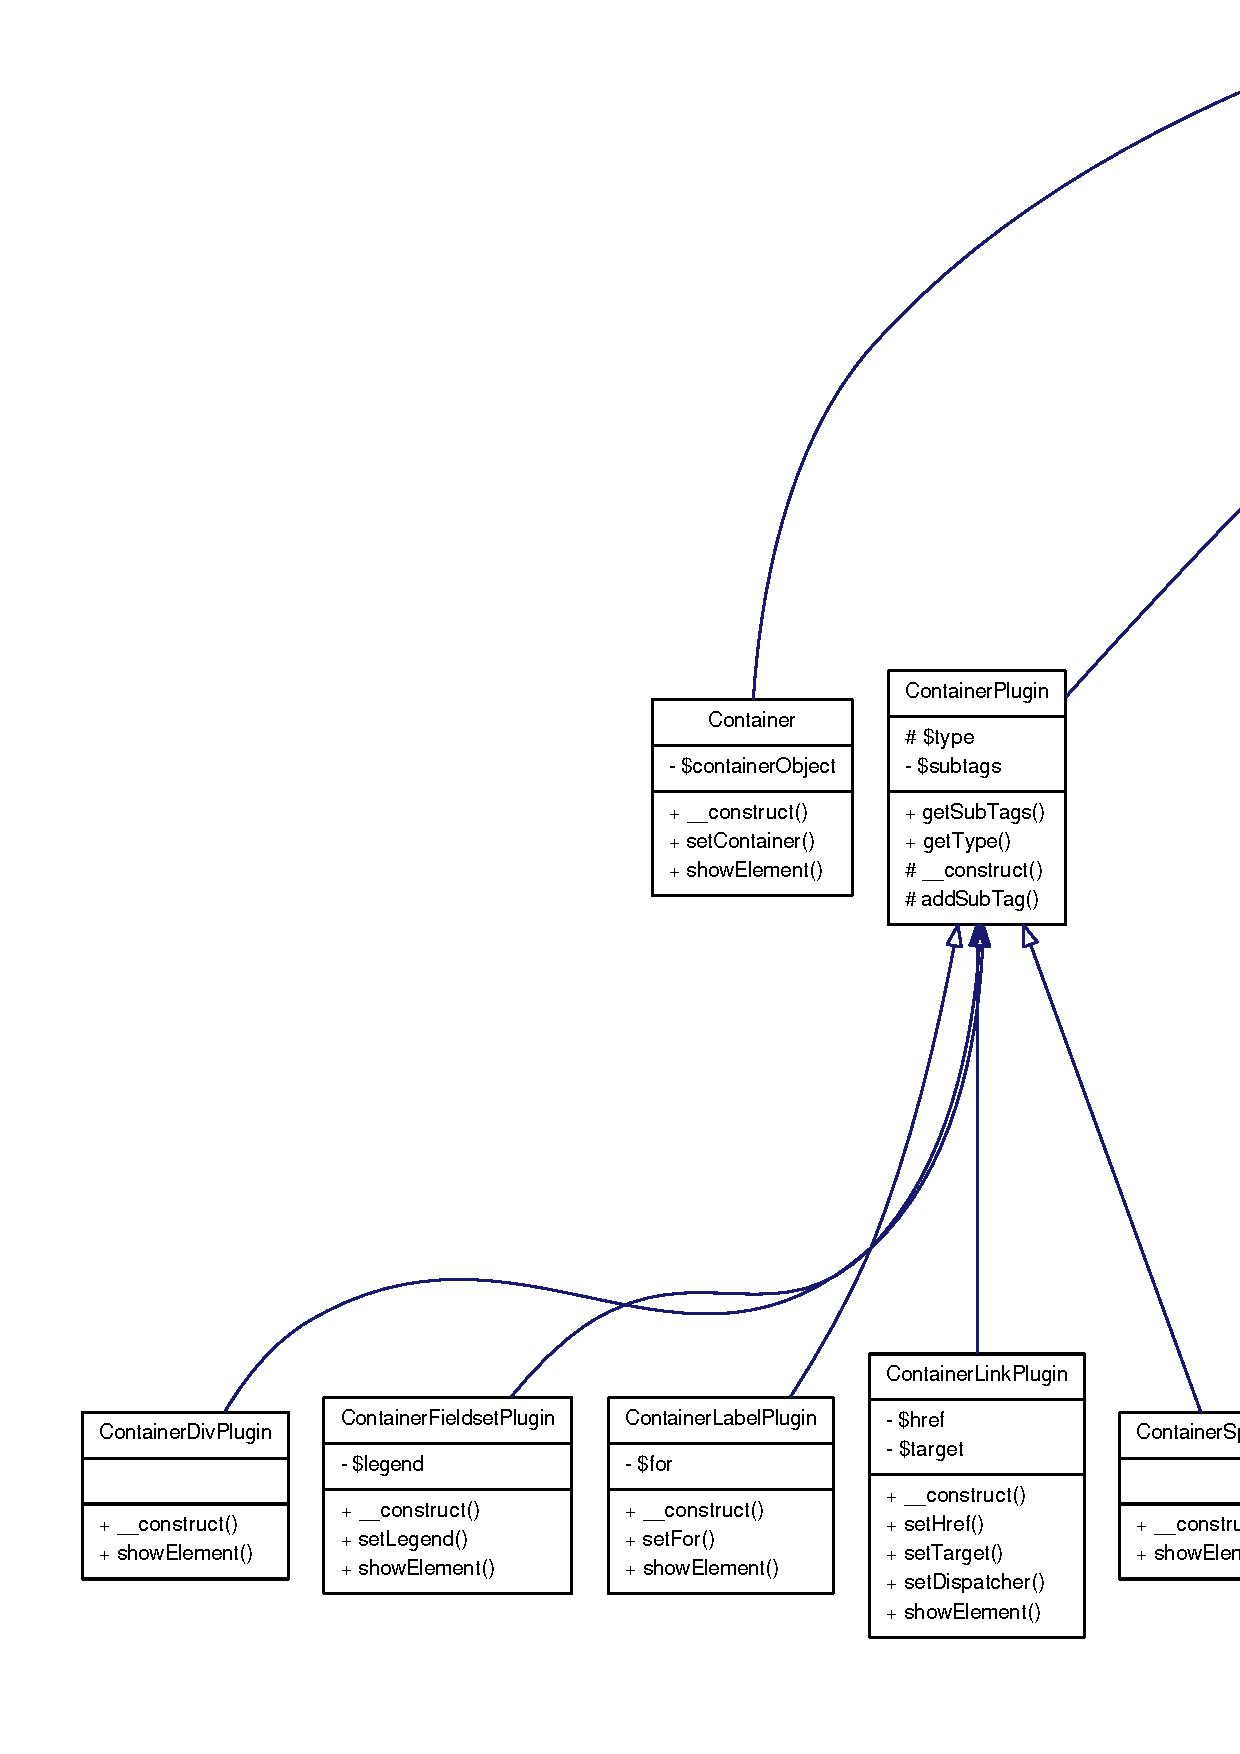
\includegraphics[width=400pt]{classBaseElement__inherit__graph}
\end{center}
\end{figure}


Collaboration diagram for BaseElement:\nopagebreak
\begin{figure}[H]
\begin{center}
\leavevmode
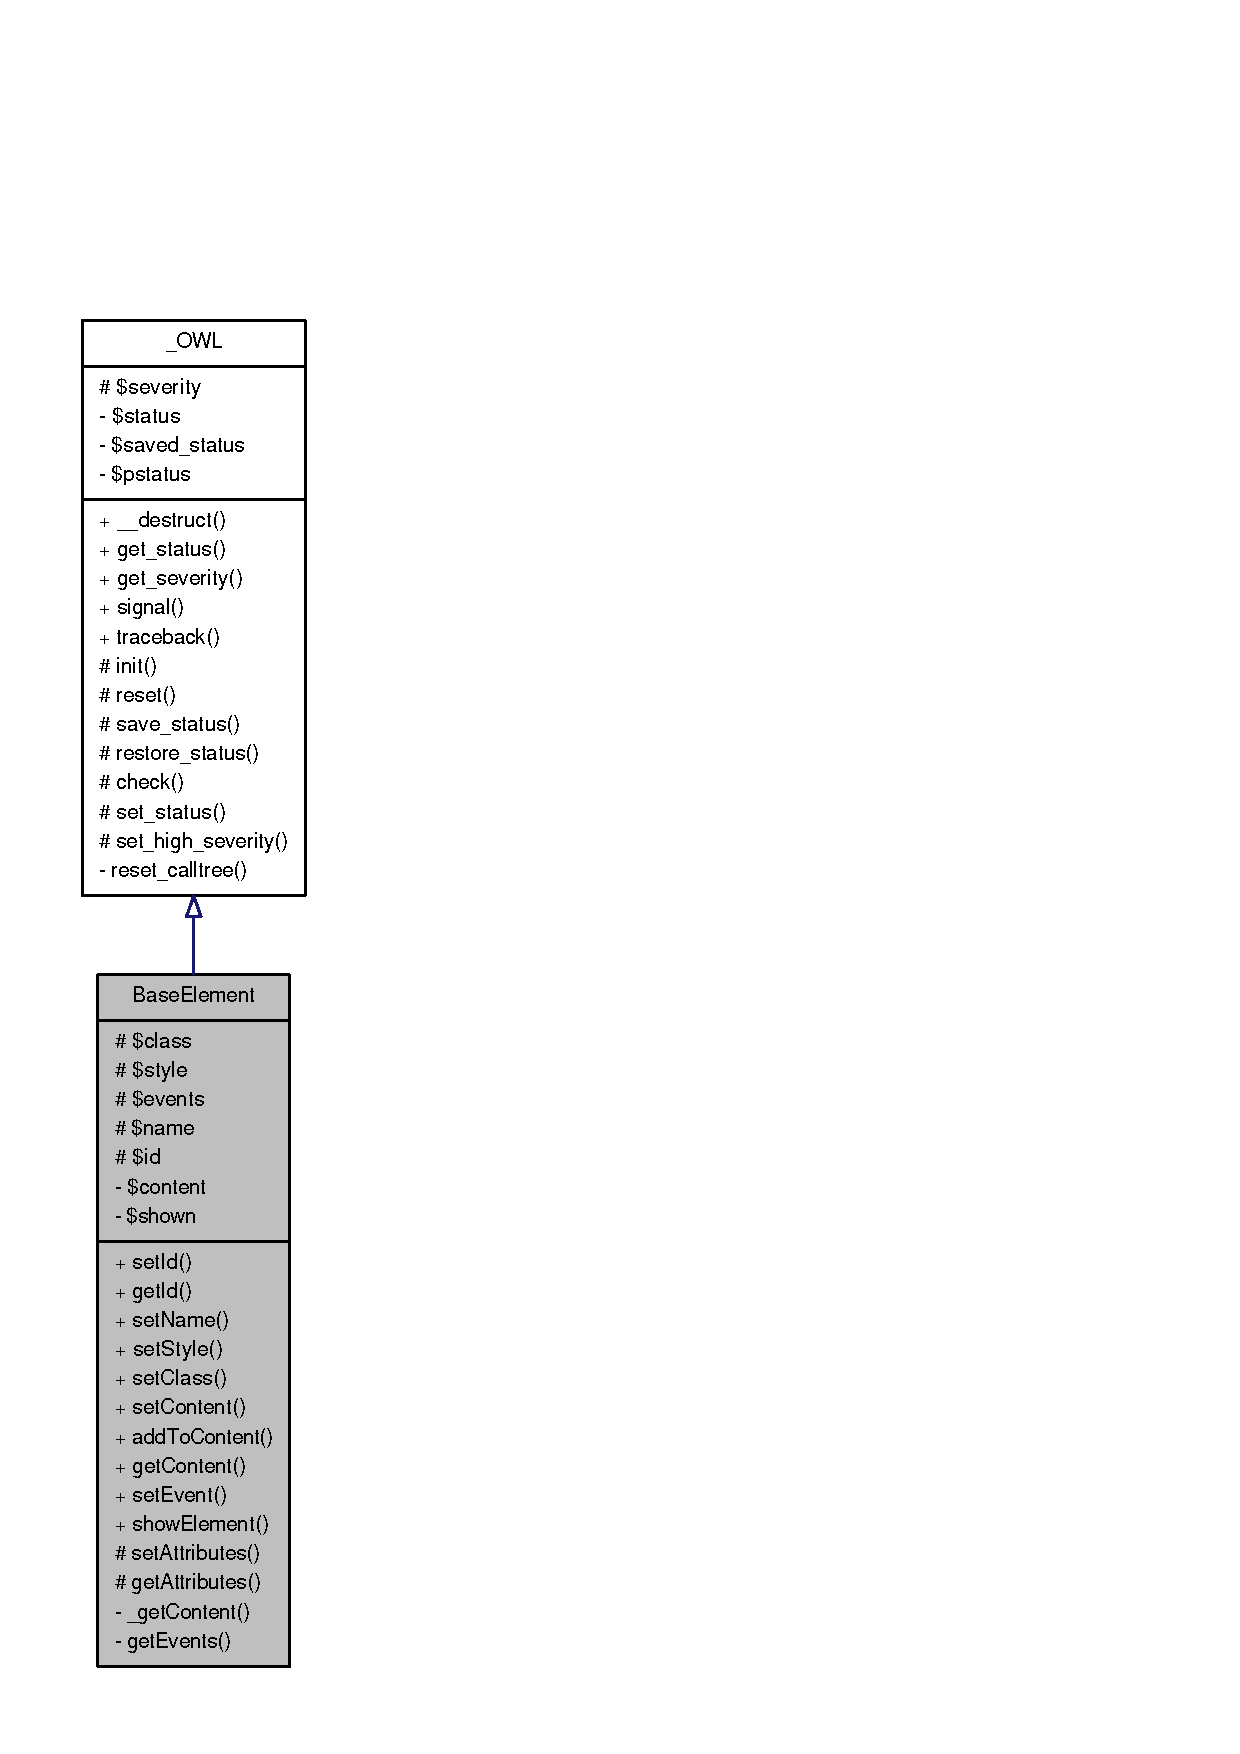
\includegraphics[height=600pt]{classBaseElement__coll__graph}
\end{center}
\end{figure}
\subsection*{Public Member Functions}
\begin{DoxyCompactItemize}
\item 
\hyperlink{classBaseElement_a0c1ce3d1684ecb78960cf7a97278494e}{setId} (\$\_\-value)
\item 
\hyperlink{classBaseElement_a4a7aa583ee21af392908d7fd42fde790}{getId} ()
\item 
\hyperlink{classBaseElement_a39bafb3609d10048920c20242c2a04c5}{setName} (\$\_\-value)
\item 
\hyperlink{classBaseElement_a6b2b9ff69f6e92db82f91d9c55cda697}{setStyle} (\$\_\-value)
\item 
\hyperlink{classBaseElement_af6597b30fa9798878f6290271043dfa2}{setClass} (\$\_\-value)
\item 
\hyperlink{classBaseElement_a164a9c6e4ee68afa0ad343942ba54d28}{setContent} (\&\$\_\-content)
\item 
\hyperlink{classBaseElement_af8c86b93bcdcfbc415bf96c622dc5516}{getContent} ()
\item 
\hyperlink{classBaseElement_ad5789f45f16aaa144716ee8558069c31}{setEvent} (\$\_\-event, \$\_\-action, \$\_\-add=false)
\item 
\hyperlink{classBaseElement_a63634d81fad745e3b72cda0100afebea}{showElement} ()
\item 
\hyperlink{class__OWL_a99ec771fa2c5c279f80152cc09e489a8}{get\_\-status} ()
\item 
\hyperlink{class__OWL_adf9509ef96858be7bdd9414c5ef129aa}{get\_\-severity} (\$status=null)
\item 
\hyperlink{class__OWL_a51ba4a16409acf2a2f61f286939091a5}{signal} (\$level=\hyperlink{owl_8severitycodes_8php_a139328861128689f2f4def6a399d9057}{OWL\_\-INFO}, \&\$text=false)
\item 
\hyperlink{class__OWL_aa29547995d6741b7d2b90c1d4ea99a13}{traceback} (\&\$text=false, \$depth=0)
\end{DoxyCompactItemize}
\subsection*{Protected Member Functions}
\begin{DoxyCompactItemize}
\item 
\hyperlink{classBaseElement_aa623b042d23a5b77add8b3c452ec5855}{setAttributes} (\$\_\-attribs)
\item 
\hyperlink{classBaseElement_ae8237038633fc53db818f36da1940297}{getAttributes} (\$\_\-ignore=array())
\item 
\hyperlink{class__OWL_ae0ef3ded56e8a6b34b6461e5a721cd3e}{init} ()
\item 
\hyperlink{class__OWL_a2f2a042bcf31965194c03033df0edc9b}{reset} ()
\item 
\hyperlink{class__OWL_a9e49b9c76fbc021b244c6915ea536d71}{save\_\-status} ()
\item 
\hyperlink{class__OWL_a465eeaf40edd9f9c848841700c32ce55}{restore\_\-status} ()
\item 
\hyperlink{class__OWL_ad6f4f6946f40199dd0333cf219fa500e}{check} (\&\$object, \$level)
\item 
\hyperlink{class__OWL_aea912d0ede9b3c2a69b79072d94d4787}{set\_\-status} (\$status, \$params=array())
\item 
\hyperlink{class__OWL_a576829692a3b66e3d518853bf43abae3}{set\_\-high\_\-severity} (\&\$object=null)
\end{DoxyCompactItemize}
\subsection*{Protected Attributes}
\begin{DoxyCompactItemize}
\item 
\hyperlink{classBaseElement_a99976a8e967db92e7800309f359b0803}{\$class} = ''
\item 
\hyperlink{classBaseElement_a429a3d642dd95f30e1059ef29564b87d}{\$style} = ''
\item 
\hyperlink{classBaseElement_a02cebe45d277b4ff8f29db08bad371ba}{\$events} = array()
\item 
\hyperlink{classBaseElement_a30b8cff187a9de659a70daf287d66f45}{\$name} = ''
\item 
\hyperlink{classBaseElement_a11b6989c43b53869a09f5ce65aa55b45}{\$id} = ''
\item 
\hyperlink{class__OWL_ad26b40a9dbbacb33e299b17826f8327c}{\$severity}
\end{DoxyCompactItemize}
\subsection*{Private Member Functions}
\begin{DoxyCompactItemize}
\item 
\hyperlink{classBaseElement_a852277a83d867417f2e39e8a2483bac7}{getEvents} ()
\end{DoxyCompactItemize}
\subsection*{Private Attributes}
\begin{DoxyCompactItemize}
\item 
\hyperlink{classBaseElement_ac2c7999af8528ffd86f3f1864028948a}{\$content}
\end{DoxyCompactItemize}


\subsection{Detailed Description}
DOM Element base class. Abstract base class for all DOM elements \begin{DoxyAuthor}{Author}
Oscar van Eijk, Oveas Functionality Provider 
\end{DoxyAuthor}
\begin{DoxyVersion}{Version}
Aug 29, 2008 -\/-\/ O van Eijk -\/-\/ initial version 
\end{DoxyVersion}


\subsection{Member Function Documentation}
\index{BaseElement@{BaseElement}!check@{check}}
\index{check@{check}!BaseElement@{BaseElement}}
\subsubsection[{check}]{\setlength{\rightskip}{0pt plus 5cm}\_\-OWL::check (
\begin{DoxyParamCaption}
\item[{\&\$}]{ object, }
\item[{\$}]{ level}
\end{DoxyParamCaption}
)\hspace{0.3cm}{\ttfamily  \mbox{[}protected, inherited\mbox{]}}}\label{class__OWL_ad6f4f6946f40199dd0333cf219fa500e}
This is a helper function for lazy developers. Some checks have to be made quite often, this is a kinda macro to handle that. It compares the own severity level with that of a given object. If the highest level is above a given max, a traceback and reset are performed.


\begin{DoxyParams}{Parameters}
\item[\mbox{\tt[in]} {\em \$object}]Pointer to an object to check against \item[\mbox{\tt[in]} {\em \$level}]The maximum severity level \end{DoxyParams}
\begin{DoxyReturn}{Returns}
True if the severity level was correct ( below the max), otherwise false 
\end{DoxyReturn}


References \_\-OWL::reset(), \_\-OWL::set\_\-high\_\-severity(), and \_\-OWL::traceback().



Referenced by SessionHandler::write().

\index{BaseElement@{BaseElement}!get\_\-severity@{get\_\-severity}}
\index{get\_\-severity@{get\_\-severity}!BaseElement@{BaseElement}}
\subsubsection[{get\_\-severity}]{\setlength{\rightskip}{0pt plus 5cm}\_\-OWL::get\_\-severity (
\begin{DoxyParamCaption}
\item[{\$}]{ status = {\ttfamily null}}
\end{DoxyParamCaption}
)\hspace{0.3cm}{\ttfamily  \mbox{[}inherited\mbox{]}}}\label{class__OWL_adf9509ef96858be7bdd9414c5ef129aa}
Get the current object severity level.


\begin{DoxyParams}{Parameters}
\item[\mbox{\tt[in]} {\em \$status}]An optional parameter to check an other status code i.s.o the object's current status. \end{DoxyParams}
\begin{DoxyReturn}{Returns}
Status severity level 
\end{DoxyReturn}


References \_\-OWL::\$status.



Referenced by LogHandler::compose\_\-message(), LogHandler::log(), and DataHandler::set\_\-key().

\index{BaseElement@{BaseElement}!get\_\-status@{get\_\-status}}
\index{get\_\-status@{get\_\-status}!BaseElement@{BaseElement}}
\subsubsection[{get\_\-status}]{\setlength{\rightskip}{0pt plus 5cm}\_\-OWL::get\_\-status (
\begin{DoxyParamCaption}
{}
\end{DoxyParamCaption}
)\hspace{0.3cm}{\ttfamily  \mbox{[}final, inherited\mbox{]}}}\label{class__OWL_a99ec771fa2c5c279f80152cc09e489a8}
Get the current object status.

\begin{DoxyReturn}{Returns}
Object's status code 
\end{DoxyReturn}


Referenced by SchemeHandler::compare().

\index{BaseElement@{BaseElement}!getAttributes@{getAttributes}}
\index{getAttributes@{getAttributes}!BaseElement@{BaseElement}}
\subsubsection[{getAttributes}]{\setlength{\rightskip}{0pt plus 5cm}BaseElement::getAttributes (
\begin{DoxyParamCaption}
\item[{\$}]{ \_\-ignore = {\ttfamily array()}}
\end{DoxyParamCaption}
)\hspace{0.3cm}{\ttfamily  \mbox{[}protected\mbox{]}}}\label{classBaseElement_ae8237038633fc53db818f36da1940297}
Return the general element attributes that are set 
\begin{DoxyParams}{Parameters}
\item[\mbox{\tt[in]} {\em \$\_\-ignore}]Array with attributes names that should be ignored \end{DoxyParams}
\begin{DoxyReturn}{Returns}
string attributes in HTML format (' fld=\char`\"{}value\char`\"{}...) 
\end{DoxyReturn}


References getEvents().



Referenced by FormFieldPlugin::getGenericFieldAttributes(), Form::openForm(), Tablerow::showElement(), Tablecell::showElement(), Table::showElement(), and Container::showElement().

\index{BaseElement@{BaseElement}!getContent@{getContent}}
\index{getContent@{getContent}!BaseElement@{BaseElement}}
\subsubsection[{getContent}]{\setlength{\rightskip}{0pt plus 5cm}BaseElement::getContent (
\begin{DoxyParamCaption}
{}
\end{DoxyParamCaption}
)}\label{classBaseElement_af8c86b93bcdcfbc415bf96c622dc5516}
Get the content of the current container, which can be plain HTML or an object, in which case the HTML will be retrieved from the object here. Enter description here ... 

Referenced by Tablecell::showElement(), and Container::showElement().

\index{BaseElement@{BaseElement}!getEvents@{getEvents}}
\index{getEvents@{getEvents}!BaseElement@{BaseElement}}
\subsubsection[{getEvents}]{\setlength{\rightskip}{0pt plus 5cm}BaseElement::getEvents (
\begin{DoxyParamCaption}
{}
\end{DoxyParamCaption}
)\hspace{0.3cm}{\ttfamily  \mbox{[}private\mbox{]}}}\label{classBaseElement_a852277a83d867417f2e39e8a2483bac7}
Return the HTML attribute list for events that where set for this element. \begin{DoxyReturn}{Returns}
string, HTML code 
\end{DoxyReturn}


Referenced by getAttributes().

\index{BaseElement@{BaseElement}!getId@{getId}}
\index{getId@{getId}!BaseElement@{BaseElement}}
\subsubsection[{getId}]{\setlength{\rightskip}{0pt plus 5cm}BaseElement::getId (
\begin{DoxyParamCaption}
{}
\end{DoxyParamCaption}
)}\label{classBaseElement_a4a7aa583ee21af392908d7fd42fde790}
Get the element's HTML ID

\begin{DoxyReturn}{Returns}
The ID 
\end{DoxyReturn}
\index{BaseElement@{BaseElement}!init@{init}}
\index{init@{init}!BaseElement@{BaseElement}}
\subsubsection[{init}]{\setlength{\rightskip}{0pt plus 5cm}\_\-OWL::init (
\begin{DoxyParamCaption}
{}
\end{DoxyParamCaption}
)\hspace{0.3cm}{\ttfamily  \mbox{[}protected, inherited\mbox{]}}}\label{class__OWL_ae0ef3ded56e8a6b34b6461e5a721cd3e}
This function should be called by all constuctors. It initializes the general characteristics. Status is 'warning' by default, it's up to the contructor to set a proper status; if it's still 'warning', this $\ast$might$\ast$ indicate something went wrong. 

References OWL::factory().



Referenced by FormFieldPlugin::\_\-\_\-construct(), Tablerow::\_\-\_\-construct(), Tablecell::\_\-\_\-construct(), Table::\_\-\_\-construct(), ContainerPlugin::\_\-\_\-construct(), Container::\_\-\_\-construct(), UserHandler::\_\-\_\-construct(), SessionHandler::\_\-\_\-construct(), SchemeHandler::\_\-\_\-construct(), LogHandler::\_\-\_\-construct(), ImageHandler::\_\-\_\-construct(), FormHandler::\_\-\_\-construct(), FileHandler::\_\-\_\-construct(), DbHandler::\_\-\_\-construct(), OWL::\_\-\_\-construct(), Form::\_\-\_\-construct(), Dispatcher::\_\-\_\-construct(), and DataHandler::DataHandler().

\index{BaseElement@{BaseElement}!reset@{reset}}
\index{reset@{reset}!BaseElement@{BaseElement}}
\subsubsection[{reset}]{\setlength{\rightskip}{0pt plus 5cm}\_\-OWL::reset (
\begin{DoxyParamCaption}
{}
\end{DoxyParamCaption}
)\hspace{0.3cm}{\ttfamily  \mbox{[}protected, inherited\mbox{]}}}\label{class__OWL_a2f2a042bcf31965194c03033df0edc9b}
General reset function for all objects. Should be called after each non-\/fatal error 

Reimplemented in \hyperlink{classDbHandler_a9982df4830f05803935bb31bac7fae3d}{DbHandler}, and \hyperlink{classSchemeHandler_aa25feb4a70d67b3d571904be4b2f50bc}{SchemeHandler}.



References \_\-OWL::reset\_\-calltree().



Referenced by \_\-OWL::check(), SessionHandler::read(), DataHandler::reset(), and \_\-OWL::set\_\-status().

\index{BaseElement@{BaseElement}!restore\_\-status@{restore\_\-status}}
\index{restore\_\-status@{restore\_\-status}!BaseElement@{BaseElement}}
\subsubsection[{restore\_\-status}]{\setlength{\rightskip}{0pt plus 5cm}\_\-OWL::restore\_\-status (
\begin{DoxyParamCaption}
{}
\end{DoxyParamCaption}
)\hspace{0.3cm}{\ttfamily  \mbox{[}protected, inherited\mbox{]}}}\label{class__OWL_a465eeaf40edd9f9c848841700c32ce55}
Restore the previously saved status object and destroy the copy 

References \_\-OWL::set\_\-status().



Referenced by UserHandler::logout().

\index{BaseElement@{BaseElement}!save\_\-status@{save\_\-status}}
\index{save\_\-status@{save\_\-status}!BaseElement@{BaseElement}}
\subsubsection[{save\_\-status}]{\setlength{\rightskip}{0pt plus 5cm}\_\-OWL::save\_\-status (
\begin{DoxyParamCaption}
{}
\end{DoxyParamCaption}
)\hspace{0.3cm}{\ttfamily  \mbox{[}protected, inherited\mbox{]}}}\label{class__OWL_a9e49b9c76fbc021b244c6915ea536d71}
Create a copy of the status object 

Referenced by UserHandler::logout().

\index{BaseElement@{BaseElement}!set\_\-high\_\-severity@{set\_\-high\_\-severity}}
\index{set\_\-high\_\-severity@{set\_\-high\_\-severity}!BaseElement@{BaseElement}}
\subsubsection[{set\_\-high\_\-severity}]{\setlength{\rightskip}{0pt plus 5cm}\_\-OWL::set\_\-high\_\-severity (
\begin{DoxyParamCaption}
\item[{\&\$}]{ object = {\ttfamily null}}
\end{DoxyParamCaption}
)\hspace{0.3cm}{\ttfamily  \mbox{[}protected, inherited\mbox{]}}}\label{class__OWL_a576829692a3b66e3d518853bf43abae3}
Compare the severity level of the current object with a given one and set my statuspointer to the object with the highest level. 

Referenced by \_\-OWL::check(), DataHandler::db(), DataHandler::prepare(), and SessionHandler::read().

\index{BaseElement@{BaseElement}!set\_\-status@{set\_\-status}}
\index{set\_\-status@{set\_\-status}!BaseElement@{BaseElement}}
\subsubsection[{set\_\-status}]{\setlength{\rightskip}{0pt plus 5cm}\_\-OWL::set\_\-status (
\begin{DoxyParamCaption}
\item[{\$}]{ status, }
\item[{\$}]{ params = {\ttfamily array~()}}
\end{DoxyParamCaption}
)\hspace{0.3cm}{\ttfamily  \mbox{[}final, protected, inherited\mbox{]}}}\label{class__OWL_aea912d0ede9b3c2a69b79072d94d4787}
Set the current object status to the specified value.


\begin{DoxyParams}{Parameters}
\item[\mbox{\tt[in]} {\em \$status}]\hyperlink{classOWL}{OWL} status code \item[\mbox{\tt[in]} {\em \$params}]\end{DoxyParams}


References \$GLOBALS, \_\-OWL::\$status, ConfigHandler::get(), Register::get\_\-code(), \_\-OWL::reset(), and \_\-OWL::signal().



Referenced by Container::\_\-\_\-construct(), UserHandler::\_\-\_\-construct(), SessionHandler::\_\-\_\-construct(), SchemeHandler::\_\-\_\-construct(), ImageHandler::\_\-\_\-construct(), FormHandler::\_\-\_\-construct(), FileHandler::\_\-\_\-construct(), DbHandler::\_\-\_\-construct(), Form::\_\-\_\-construct(), Form::addField(), SchemeHandler::alter\_\-scheme(), FileHandler::close(), DbHandler::connect(), DbHandler::create(), SchemeHandler::create\_\-scheme(), DataHandler::DataHandler(), SchemeHandler::define\_\-index(), SchemeHandler::define\_\-scheme(), Dispatcher::dispatch(), FormHandler::get(), DataHandler::get(), SchemeHandler::get\_\-table\_\-columns(), SchemeHandler::get\_\-table\_\-indexes(), UserHandler::login(), FileHandler::open(), DbHandler::open(), LogHandler::open\_\-logfile(), DataHandler::prepare(), DbHandler::prepare\_\-delete(), DbHandler::prepare\_\-insert(), DbHandler::prepare\_\-read(), DbHandler::prepare\_\-update(), DbHandler::read(), FileHandler::read\_\-line(), UserHandler::read\_\-userdata(), \_\-OWL::restore\_\-status(), SchemeHandler::scheme(), FormHandler::set(), DataHandler::set(), DataHandler::set\_\-join(), DataHandler::set\_\-key(), setAttributes(), setContent(), Form::setEncoding(), Form::setFieldAttributes(), FormFieldTextPlugin::setMaxsize(), Form::setMethod(), FormFieldRadioPlugin::setSelected(), FormFieldTextPlugin::setSize(), FormFieldSelectPlugin::setSize(), FormFieldSelectPlugin::setValue(), FormFieldRadioPlugin::setValue(), Form::showField(), SchemeHandler::table\_\-description(), SchemeHandler::validate\_\-scheme(), and DbHandler::write().

\index{BaseElement@{BaseElement}!setAttributes@{setAttributes}}
\index{setAttributes@{setAttributes}!BaseElement@{BaseElement}}
\subsubsection[{setAttributes}]{\setlength{\rightskip}{0pt plus 5cm}BaseElement::setAttributes (
\begin{DoxyParamCaption}
\item[{\$}]{ \_\-attribs}
\end{DoxyParamCaption}
)\hspace{0.3cm}{\ttfamily  \mbox{[}protected\mbox{]}}}\label{classBaseElement_aa623b042d23a5b77add8b3c452ec5855}
Set the attributes of the DOM element by calling the 'set$<$Attrib$>$' method for this class. 
\begin{DoxyParams}{Parameters}
\item[\mbox{\tt[in]} {\em \$\_\-attribs}]Array with attributes in the format attrib=$>$value \end{DoxyParams}
\begin{DoxyReturn}{Returns}
Severity level. The status increased when a set$<$Attrib$>$ method does not exist. 
\end{DoxyReturn}


Reimplemented in \hyperlink{classTablecell_a91a8264df222cc44b77ceaf7282a400e}{Tablecell}, and \hyperlink{classTablerow_aece4cad0834c299d7e03030e945aea3a}{Tablerow}.



References \_\-OWL::set\_\-status().



Referenced by Table::\_\-\_\-construct(), and Container::\_\-\_\-construct().

\index{BaseElement@{BaseElement}!setClass@{setClass}}
\index{setClass@{setClass}!BaseElement@{BaseElement}}
\subsubsection[{setClass}]{\setlength{\rightskip}{0pt plus 5cm}BaseElement::setClass (
\begin{DoxyParamCaption}
\item[{\$}]{ \_\-value}
\end{DoxyParamCaption}
)}\label{classBaseElement_af6597b30fa9798878f6290271043dfa2}
Set the element Class 
\begin{DoxyParams}{Parameters}
\item[\mbox{\tt[in]} {\em \$\_\-value}]Class name \end{DoxyParams}
\index{BaseElement@{BaseElement}!setContent@{setContent}}
\index{setContent@{setContent}!BaseElement@{BaseElement}}
\subsubsection[{setContent}]{\setlength{\rightskip}{0pt plus 5cm}BaseElement::setContent (
\begin{DoxyParamCaption}
\item[{\&\$}]{ \_\-content}
\end{DoxyParamCaption}
)}\label{classBaseElement_a164a9c6e4ee68afa0ad343942ba54d28}
Fill the content for a container. Existing content (e.g. set during instantiation) will be overwritten. 
\begin{DoxyParams}{Parameters}
\item[\mbox{\tt[in]} {\em \$\_\-content}]Reference to the content, which can be HTML code or an object, of which the \hyperlink{classBaseElement_a63634d81fad745e3b72cda0100afebea}{showElement()} method will be called to retrieve the HTML. \end{DoxyParams}


References \_\-OWL::set\_\-status().



Referenced by Tablecell::\_\-\_\-construct(), and Container::\_\-\_\-construct().

\index{BaseElement@{BaseElement}!setEvent@{setEvent}}
\index{setEvent@{setEvent}!BaseElement@{BaseElement}}
\subsubsection[{setEvent}]{\setlength{\rightskip}{0pt plus 5cm}BaseElement::setEvent (
\begin{DoxyParamCaption}
\item[{\$}]{ \_\-event, }
\item[{\$}]{ \_\-action, }
\item[{\$}]{ \_\-add = {\ttfamily false}}
\end{DoxyParamCaption}
)}\label{classBaseElement_ad5789f45f16aaa144716ee8558069c31}
Add an event to the events array 
\begin{DoxyParams}{Parameters}
\item[\mbox{\tt[in]} {\em \$\_\-event}]Javascript event name (onXxx) \item[\mbox{\tt[in]} {\em \$\_\-action}]Javascript function or code \item[\mbox{\tt[in]} {\em \$\_\-add}]Boolean; when true, the action will be added if the event name already exists. Default is false; overwrite the action for this event. \end{DoxyParams}
\index{BaseElement@{BaseElement}!setId@{setId}}
\index{setId@{setId}!BaseElement@{BaseElement}}
\subsubsection[{setId}]{\setlength{\rightskip}{0pt plus 5cm}BaseElement::setId (
\begin{DoxyParamCaption}
\item[{\$}]{ \_\-value}
\end{DoxyParamCaption}
)}\label{classBaseElement_a0c1ce3d1684ecb78960cf7a97278494e}
Set the element ID 
\begin{DoxyParams}{Parameters}
\item[\mbox{\tt[in]} {\em \$\_\-value}]Identification \end{DoxyParams}


Referenced by setName().

\index{BaseElement@{BaseElement}!setName@{setName}}
\index{setName@{setName}!BaseElement@{BaseElement}}
\subsubsection[{setName}]{\setlength{\rightskip}{0pt plus 5cm}BaseElement::setName (
\begin{DoxyParamCaption}
\item[{\$}]{ \_\-value}
\end{DoxyParamCaption}
)}\label{classBaseElement_a39bafb3609d10048920c20242c2a04c5}
Set the element name 
\begin{DoxyParams}{Parameters}
\item[\mbox{\tt[in]} {\em \$\_\-value}]Element name \end{DoxyParams}


References setId().

\index{BaseElement@{BaseElement}!setStyle@{setStyle}}
\index{setStyle@{setStyle}!BaseElement@{BaseElement}}
\subsubsection[{setStyle}]{\setlength{\rightskip}{0pt plus 5cm}BaseElement::setStyle (
\begin{DoxyParamCaption}
\item[{\$}]{ \_\-value}
\end{DoxyParamCaption}
)}\label{classBaseElement_a6b2b9ff69f6e92db82f91d9c55cda697}
Set the element style 
\begin{DoxyParams}{Parameters}
\item[\mbox{\tt[in]} {\em \$\_\-value}]Element style \end{DoxyParams}
\index{BaseElement@{BaseElement}!showElement@{showElement}}
\index{showElement@{showElement}!BaseElement@{BaseElement}}
\subsubsection[{showElement}]{\setlength{\rightskip}{0pt plus 5cm}BaseElement::showElement (
\begin{DoxyParamCaption}
{}
\end{DoxyParamCaption}
)\hspace{0.3cm}{\ttfamily  \mbox{[}abstract\mbox{]}}}\label{classBaseElement_a63634d81fad745e3b72cda0100afebea}
This function must be implemented by all elements. \begin{DoxyReturn}{Returns}
The implementation must return a textstring with the complete HTML code to display the element 
\end{DoxyReturn}


Reimplemented in \hyperlink{classForm_aeac5855c8b2406c34090a621d59df664}{Form}, \hyperlink{classContainer_a966af30a8c244fbc2ee61648fa59ffe3}{Container}, \hyperlink{classTable_a71c094dc93aee06ee427f2d53a6691c0}{Table}, \hyperlink{classTablecell_a3dd7511a61bfb8100ff293435685209d}{Tablecell}, \hyperlink{classTablerow_a050c4f377fec4b9554734ff339aaade8}{Tablerow}, \hyperlink{classContainerDivPlugin_a4d9cb8fa601b51f951e5f90aad4d1a3c}{ContainerDivPlugin}, \hyperlink{classContainerFieldsetPlugin_aacca071df123a3068b0b6b8ed5dbdb83}{ContainerFieldsetPlugin}, \hyperlink{classContainerLabelPlugin_ab725a7631eae2f0467a1c04bbd5081d7}{ContainerLabelPlugin}, \hyperlink{classContainerSpanPlugin_a5a1d46ade3182c9cd270e6e01844e30c}{ContainerSpanPlugin}, \hyperlink{classFormFieldButtonPlugin_a029b1662ddc1652b2a571cb2b72421b7}{FormFieldButtonPlugin}, \hyperlink{classFormFieldCheckboxPlugin_a0bed3773bd415fc026d042102c1d4740}{FormFieldCheckboxPlugin}, \hyperlink{classFormFieldPlugin_a3983c0e5035930d864d40e606ab3670b}{FormFieldPlugin}, \hyperlink{classFormFieldRadioPlugin_aade41bf9d88869342c319954da8df608}{FormFieldRadioPlugin}, \hyperlink{classFormFieldSelectPlugin_a65df2919c0789f499302f75ec2356876}{FormFieldSelectPlugin}, \hyperlink{classFormFieldTextPlugin_ac6cee64e91f04b380e948973026bff4e}{FormFieldTextPlugin}, and \hyperlink{classFormFieldTextareaPlugin_ad2b4186a948dded848826a4870e7713b}{FormFieldTextareaPlugin}.

\index{BaseElement@{BaseElement}!signal@{signal}}
\index{signal@{signal}!BaseElement@{BaseElement}}
\subsubsection[{signal}]{\setlength{\rightskip}{0pt plus 5cm}\_\-OWL::signal (
\begin{DoxyParamCaption}
\item[{\$}]{ level = {\ttfamily {\bf OWL\_\-INFO}}, }
\item[{\&\$}]{ text = {\ttfamily false}}
\end{DoxyParamCaption}
)\hspace{0.3cm}{\ttfamily  \mbox{[}inherited\mbox{]}}}\label{class__OWL_a51ba4a16409acf2a2f61f286939091a5}
Display the message for the current object status


\begin{DoxyParams}{Parameters}
\item[\mbox{\tt[in]} {\em \$level}]An optional severity level; message will only be displayed when it is at least of this level. \item[\mbox{\tt[out]} {\em \$text}]If this parameter is given, the message text is returned in this string instead of echood. \end{DoxyParams}
\begin{DoxyReturn}{Returns}
The severity level for this object 
\end{DoxyReturn}


References ConfigHandler::get().



Referenced by \_\-OWL::set\_\-status(), and \_\-OWL::traceback().

\index{BaseElement@{BaseElement}!traceback@{traceback}}
\index{traceback@{traceback}!BaseElement@{BaseElement}}
\subsubsection[{traceback}]{\setlength{\rightskip}{0pt plus 5cm}\_\-OWL::traceback (
\begin{DoxyParamCaption}
\item[{\&\$}]{ text = {\ttfamily false}, }
\item[{\$}]{ depth = {\ttfamily 0}}
\end{DoxyParamCaption}
)\hspace{0.3cm}{\ttfamily  \mbox{[}inherited\mbox{]}}}\label{class__OWL_aa29547995d6741b7d2b90c1d4ea99a13}
If somehwere in the nested calls an error occured, we can traceback the original failing object with this function and signal the message.


\begin{DoxyParams}{Parameters}
\item[\mbox{\tt[out]} {\em \$text}]Optional variable in which the message text can be stored. If not given, the text will be written to standard output \item[\mbox{\tt[in]} {\em \$depth}]This paramater should be initially empty. It calculates the depth in recursive calls. \end{DoxyParams}
\begin{DoxyReturn}{Returns}
Severity code of the failing object 
\end{DoxyReturn}


References \_\-OWL::signal().



Referenced by \_\-OWL::check(), UserHandler::login(), and SessionHandler::read().



\subsection{Member Data Documentation}
\index{BaseElement@{BaseElement}!\$class@{\$class}}
\index{\$class@{\$class}!BaseElement@{BaseElement}}
\subsubsection[{\$class}]{\setlength{\rightskip}{0pt plus 5cm}BaseElement::\$class = ''\hspace{0.3cm}{\ttfamily  \mbox{[}protected\mbox{]}}}\label{classBaseElement_a99976a8e967db92e7800309f359b0803}
Class specification \index{BaseElement@{BaseElement}!\$content@{\$content}}
\index{\$content@{\$content}!BaseElement@{BaseElement}}
\subsubsection[{\$content}]{\setlength{\rightskip}{0pt plus 5cm}BaseElement::\$content\hspace{0.3cm}{\ttfamily  \mbox{[}private\mbox{]}}}\label{classBaseElement_ac2c7999af8528ffd86f3f1864028948a}
Content for a container \index{BaseElement@{BaseElement}!\$events@{\$events}}
\index{\$events@{\$events}!BaseElement@{BaseElement}}
\subsubsection[{\$events}]{\setlength{\rightskip}{0pt plus 5cm}BaseElement::\$events = array()\hspace{0.3cm}{\ttfamily  \mbox{[}protected\mbox{]}}}\label{classBaseElement_a02cebe45d277b4ff8f29db08bad371ba}
Array with javascript events 

Referenced by Form::setFieldEvents().

\index{BaseElement@{BaseElement}!\$id@{\$id}}
\index{\$id@{\$id}!BaseElement@{BaseElement}}
\subsubsection[{\$id}]{\setlength{\rightskip}{0pt plus 5cm}BaseElement::\$id = ''\hspace{0.3cm}{\ttfamily  \mbox{[}protected\mbox{]}}}\label{classBaseElement_a11b6989c43b53869a09f5ce65aa55b45}
Element ID \index{BaseElement@{BaseElement}!\$name@{\$name}}
\index{\$name@{\$name}!BaseElement@{BaseElement}}
\subsubsection[{\$name}]{\setlength{\rightskip}{0pt plus 5cm}BaseElement::\$name = ''\hspace{0.3cm}{\ttfamily  \mbox{[}protected\mbox{]}}}\label{classBaseElement_a30b8cff187a9de659a70daf287d66f45}
Name of the element 

Referenced by Form::addField(), and Form::showField().

\index{BaseElement@{BaseElement}!\$severity@{\$severity}}
\index{\$severity@{\$severity}!BaseElement@{BaseElement}}
\subsubsection[{\$severity}]{\setlength{\rightskip}{0pt plus 5cm}\_\-OWL::\$severity\hspace{0.3cm}{\ttfamily  \mbox{[}protected, inherited\mbox{]}}}\label{class__OWL_ad26b40a9dbbacb33e299b17826f8327c}
Severity level of the current object status \index{BaseElement@{BaseElement}!\$style@{\$style}}
\index{\$style@{\$style}!BaseElement@{BaseElement}}
\subsubsection[{\$style}]{\setlength{\rightskip}{0pt plus 5cm}BaseElement::\$style = ''\hspace{0.3cm}{\ttfamily  \mbox{[}protected\mbox{]}}}\label{classBaseElement_a429a3d642dd95f30e1059ef29564b87d}
Element style 

The documentation for this class was generated from the following file:\begin{DoxyCompactItemize}
\item 
/home/oscar/projects/owl-\/php/src/kernel/ui/\hyperlink{class_8baseelement_8php}{class.baseelement.php}\end{DoxyCompactItemize}

\section{ConfigHandler Class Reference}
\label{classConfigHandler}\index{ConfigHandler@{ConfigHandler}}


Configuration handler.  


\subsection*{Static Public Member Functions}
\begin{DoxyCompactItemize}
\item 
static \hyperlink{classConfigHandler_af61ee6f9f793e4cd0128c02e4e28bf90}{read\_\-config} (\$file= '')
\item 
static \hyperlink{classConfigHandler_aa8f6a7516588561626efccb8be5875ce}{get} (\$item, \$default=null)
\item 
static \hyperlink{classConfigHandler_a82c10cf53f06169cee0bdc0716bc089a}{set} (\$item, \$value)
\end{DoxyCompactItemize}
\subsection*{Static Private Member Functions}
\begin{DoxyCompactItemize}
\item 
static \hyperlink{classConfigHandler_a9851c66d75db6a65c64aba5192173c14}{convert} (\$val)
\end{DoxyCompactItemize}


\subsection{Detailed Description}
Configuration handler. This abstract class reads configution from file ort database, and fills and reads the global datastructure with config items \begin{DoxyAuthor}{Author}
Oscar van Eijk, Oveas Functionality Provider 
\end{DoxyAuthor}
\begin{DoxyVersion}{Version}
Aug 20, 2008 -\/-\/ O van Eijk -\/-\/ initial version 
\end{DoxyVersion}


\subsection{Member Function Documentation}
\index{ConfigHandler@{ConfigHandler}!convert@{convert}}
\index{convert@{convert}!ConfigHandler@{ConfigHandler}}
\subsubsection[{convert}]{\setlength{\rightskip}{0pt plus 5cm}static ConfigHandler::convert (
\begin{DoxyParamCaption}
\item[{\$}]{ val}
\end{DoxyParamCaption}
)\hspace{0.3cm}{\ttfamily  \mbox{[}static, private\mbox{]}}}\label{classConfigHandler_a9851c66d75db6a65c64aba5192173c14}
Convert values in character string format to a known value


\begin{DoxyParams}{Parameters}
\item[\mbox{\tt[in]} {\em \$val}]The value as read from the config file \end{DoxyParams}
\begin{DoxyReturn}{Returns}
Value in the desired format (or as is if nothing set) 
\end{DoxyReturn}


References Register::get\_\-severity\_\-level().



Referenced by read\_\-config().

\index{ConfigHandler@{ConfigHandler}!get@{get}}
\index{get@{get}!ConfigHandler@{ConfigHandler}}
\subsubsection[{get}]{\setlength{\rightskip}{0pt plus 5cm}static ConfigHandler::get (
\begin{DoxyParamCaption}
\item[{\$}]{ item, }
\item[{\$}]{ default = {\ttfamily null}}
\end{DoxyParamCaption}
)\hspace{0.3cm}{\ttfamily  \mbox{[}static\mbox{]}}}\label{classConfigHandler_aa8f6a7516588561626efccb8be5875ce}
Return a configuration value. Note! In order to use hidden values properly, this is the ONLY way configuration values should be retrieved!


\begin{DoxyParams}{Parameters}
\item[\mbox{\tt[in]} {\em \$item}]The configuration item in the same format as it appears in the configuration file (e.g. 'group$|$subject$|$item') \item[\mbox{\tt[in]} {\em \$default}]The default value to return if the config item was not set. This defaults to 'null'; if it is anything other than null, the CONFIG\_\-NOVALUE status will not be set \end{DoxyParams}
\begin{DoxyReturn}{Returns}
Corresponding value of null when nothing was found 
\end{DoxyReturn}


References \$GLOBALS, and OWL::stat().



Referenced by SessionHandler::\_\-\_\-construct(), LogHandler::\_\-\_\-construct(), OWLException::\_\-\_\-construct(), DbHandler::\_\-\_\-construct(), User::\_\-\_\-construct(), OWLException::check\_\-hide(), LogHandler::compose\_\-message(), DbHandler::connect(), FormHandler::get(), DbHandler::get\_\-instance(), UserHandler::hash\_\-password(), UserHandler::isLoggedIn(), LogHandler::log(), OWLExceptionHandler::log\_\-exception(), UserHandler::login(), User::logout(), Register::register\_\-messages(), FormHandler::set(), LogHandler::set\_\-filename(), \_\-OWL::set\_\-status(), \_\-OWL::signal(), and OWLException::traceback().

\index{ConfigHandler@{ConfigHandler}!read\_\-config@{read\_\-config}}
\index{read\_\-config@{read\_\-config}!ConfigHandler@{ConfigHandler}}
\subsubsection[{read\_\-config}]{\setlength{\rightskip}{0pt plus 5cm}static ConfigHandler::read\_\-config (
\begin{DoxyParamCaption}
\item[{\$}]{ file = {\ttfamily ''}}
\end{DoxyParamCaption}
)\hspace{0.3cm}{\ttfamily  \mbox{[}static\mbox{]}}}\label{classConfigHandler_af61ee6f9f793e4cd0128c02e4e28bf90}
Parse the given configuration file


\begin{DoxyParams}{Parameters}
\item[\mbox{\tt[in]} {\em \$file}]Full path to the configuration file \end{DoxyParams}


References \$GLOBALS, and convert().

\index{ConfigHandler@{ConfigHandler}!set@{set}}
\index{set@{set}!ConfigHandler@{ConfigHandler}}
\subsubsection[{set}]{\setlength{\rightskip}{0pt plus 5cm}static ConfigHandler::set (
\begin{DoxyParamCaption}
\item[{\$}]{ item, }
\item[{\$}]{ value}
\end{DoxyParamCaption}
)\hspace{0.3cm}{\ttfamily  \mbox{[}static\mbox{]}}}\label{classConfigHandler_a82c10cf53f06169cee0bdc0716bc089a}
Set a configuration item. Existing values will be overwritten.


\begin{DoxyParams}{Parameters}
\item[\mbox{\tt[in]} {\em \$item}]The configuration item in the same format as it appears in the configuration file (e.g. 'group$|$subject$|$item') \item[\mbox{\tt[in]} {\em \$value}]The new value of the item \end{DoxyParams}


References \$GLOBALS.



The documentation for this class was generated from the following file:\begin{DoxyCompactItemize}
\item 
/home/oscar/projects/owl-\/php/src/kernel/so/\hyperlink{class_8confighandler_8php}{class.confighandler.php}\end{DoxyCompactItemize}

\section{DataHandler Class Reference}
\label{classDataHandler}\index{DataHandler@{DataHandler}}


The \hyperlink{classOWL}{OWL} Data object.  




Inheritance diagram for DataHandler:\nopagebreak
\begin{figure}[H]
\begin{center}
\leavevmode
\includegraphics[height=600pt]{classDataHandler__inherit__graph}
\end{center}
\end{figure}


Collaboration diagram for DataHandler:\nopagebreak
\begin{figure}[H]
\begin{center}
\leavevmode
\includegraphics[height=600pt]{classDataHandler__coll__graph}
\end{center}
\end{figure}
\subsection*{Public Member Functions}
\begin{DoxyCompactItemize}
\item 
\hyperlink{classDataHandler_a4fd274c45bf06283b05e757b7c081439}{\_\-\_\-construct} (\$tablename= '')
\item 
\hyperlink{classDataHandler_ab89e1aaad9cd0a37f1c7f13c1d9c0d57}{reset} (\$level=\hyperlink{class_8datahandler_8php_a19a99423705b41e563424ae76d7fe184}{DATA\_\-RESET\_\-PREPARE})
\item 
\hyperlink{classDataHandler_a296f26f5af1e46a49ae44110848fa031}{set} (\$variable, \$value)
\item 
\hyperlink{classDataHandler_a32ce223478b78a4ea9838a3c6ac7440c}{set\_\-key} (\$variable)
\item 
\hyperlink{classDataHandler_a435338a167a44a041af2895859abb0c9}{escape\_\-string} (\$string)
\item 
\hyperlink{classDataHandler_a7dcf85dac419f51ad4daa166c928a399}{get} (\$variable)
\item 
\hyperlink{classDataHandler_a9b77733f02e9d6281fc40df110c0ba70}{set\_\-join} (\$lvalue, \$rvalue, \$linktype= '=')
\item 
\hyperlink{classDataHandler_abcb68472abd7da8ee6296421f0a7f2e9}{set\_\-tablename} (\$tblname)
\item 
\hyperlink{classDataHandler_af3e7a17194e97300d499e9178f4913cb}{prepare} (\$type=\hyperlink{class_8datahandler_8php_ac28f74b49007773d24ca2207baac6d32}{DATA\_\-READ})
\item 
\hyperlink{classDataHandler_abb329fe5a97eb8df928aabfc8078ff23}{db} (\&\$data=false, \$line=0, \$file= '\mbox{[}unknown\mbox{]}')
\item 
\hyperlink{classDataHandler_a27db6fb8365b7def4db7bd72984a0089}{set\_\-prefix} (\$prefix)
\item 
\hyperlink{classDataHandler_a3c82ec0a40dabcc55dc203c96abf02d2}{db\_\-status} ()
\item 
\hyperlink{class__OWL_a99ec771fa2c5c279f80152cc09e489a8}{get\_\-status} ()
\item 
\hyperlink{class__OWL_adf9509ef96858be7bdd9414c5ef129aa}{get\_\-severity} (\$status=null)
\item 
\hyperlink{class__OWL_a51ba4a16409acf2a2f61f286939091a5}{signal} (\$level=\hyperlink{owl_8severitycodes_8php_a139328861128689f2f4def6a399d9057}{OWL\_\-INFO}, \&\$text=false)
\item 
\hyperlink{class__OWL_aa29547995d6741b7d2b90c1d4ea99a13}{traceback} (\&\$text=false, \$depth=0)
\end{DoxyCompactItemize}
\subsection*{Protected Member Functions}
\begin{DoxyCompactItemize}
\item 
\hyperlink{class__OWL_ae0ef3ded56e8a6b34b6461e5a721cd3e}{init} ()
\item 
\hyperlink{class__OWL_a2f2a042bcf31965194c03033df0edc9b}{reset} ()
\item 
\hyperlink{class__OWL_a9e49b9c76fbc021b244c6915ea536d71}{save\_\-status} ()
\item 
\hyperlink{class__OWL_a465eeaf40edd9f9c848841700c32ce55}{restore\_\-status} ()
\item 
\hyperlink{class__OWL_ad6f4f6946f40199dd0333cf219fa500e}{check} (\&\$object, \$level)
\item 
\hyperlink{class__OWL_aea912d0ede9b3c2a69b79072d94d4787}{set\_\-status} (\$status, \$params=array())
\item 
\hyperlink{class__OWL_a576829692a3b66e3d518853bf43abae3}{set\_\-high\_\-severity} (\&\$object=null)
\end{DoxyCompactItemize}
\subsection*{Protected Attributes}
\begin{DoxyCompactItemize}
\item 
\hyperlink{class__OWL_ad26b40a9dbbacb33e299b17826f8327c}{\$severity}
\end{DoxyCompactItemize}
\subsection*{Private Member Functions}
\begin{DoxyCompactItemize}
\item 
\hyperlink{classDataHandler_a1e4789e22370c96ae479bc3a58f30984}{find\_\-field} (\$fld, \&\$expanded)
\end{DoxyCompactItemize}
\subsection*{Private Attributes}
\begin{DoxyCompactItemize}
\item 
\hyperlink{classDataHandler_a329b5524c379e0db6c4d5ce59f3c414f}{\$owl\_\-data}
\item 
\hyperlink{classDataHandler_ada9b697f81ea82d269077f9c7445791d}{\$owl\_\-joins}
\item 
\hyperlink{classDataHandler_a8d398720bce975159b2d13ad7a941bc7}{\$owl\_\-keys}
\item 
\hyperlink{classDataHandler_a24620784bde262bdd02227962d3b9605}{\$owl\_\-tablename}
\item 
\hyperlink{classDataHandler_a3ac49aa018e0ebe4c74f5a636d455a8b}{\$owl\_\-database}
\item 
\hyperlink{classDataHandler_ae6093d21291ed3ab3183e11962452928}{\$owl\_\-prepared}
\end{DoxyCompactItemize}


\subsection{Detailed Description}
The \hyperlink{classOWL}{OWL} Data object. This class contains DB datasets \begin{DoxyAuthor}{Author}
Oscar van Eijk, Oveas Functionality Provider 
\end{DoxyAuthor}
\begin{DoxyVersion}{Version}
Aug 4, 2008 -\/-\/ O van Eijk -\/-\/ initial version 
\end{DoxyVersion}


\subsection{Constructor \& Destructor Documentation}
\index{DataHandler@{DataHandler}!\_\-\_\-construct@{\_\-\_\-construct}}
\index{\_\-\_\-construct@{\_\-\_\-construct}!DataHandler@{DataHandler}}
\subsubsection[{\_\-\_\-construct}]{\setlength{\rightskip}{0pt plus 5cm}DataHandler::\_\-\_\-construct (
\begin{DoxyParamCaption}
\item[{\$}]{ tablename = {\ttfamily ''}}
\end{DoxyParamCaption}
)}\label{classDataHandler_a4fd274c45bf06283b05e757b7c081439}
Class constructor. We don't use a standard constructor (\hyperlink{classDataHandler_a4fd274c45bf06283b05e757b7c081439}{\_\-\_\-construct()}) here, since singleton classes (using private constructors) might derive from this class. In stead we use the PHP4 compatible constructor. 
\begin{DoxyParams}{Parameters}
\item[\mbox{\tt[in]} {\em \$tablename}]Default table name for this dataset \end{DoxyParams}


References OWL::factory(), \_\-OWL::init(), and \_\-OWL::set\_\-status().



\subsection{Member Function Documentation}
\index{DataHandler@{DataHandler}!check@{check}}
\index{check@{check}!DataHandler@{DataHandler}}
\subsubsection[{check}]{\setlength{\rightskip}{0pt plus 5cm}\_\-OWL::check (
\begin{DoxyParamCaption}
\item[{\&\$}]{ object, }
\item[{\$}]{ level}
\end{DoxyParamCaption}
)\hspace{0.3cm}{\ttfamily  \mbox{[}protected, inherited\mbox{]}}}\label{class__OWL_ad6f4f6946f40199dd0333cf219fa500e}
This is a helper function for lazy developers. Some checks have to be made quite often, this is a kinda macro to handle that. It compares the own severity level with that of a given object. If the highest level is above a given max, a traceback and reset are performed.


\begin{DoxyParams}{Parameters}
\item[\mbox{\tt[in]} {\em \$object}]Pointer to an object to check against \item[\mbox{\tt[in]} {\em \$level}]The maximum severity level \end{DoxyParams}
\begin{DoxyReturn}{Returns}
True if the severity level was correct ( below the max), otherwise false 
\end{DoxyReturn}


References \_\-OWL::reset(), \_\-OWL::set\_\-high\_\-severity(), and \_\-OWL::traceback().



Referenced by SessionHandler::write().

\index{DataHandler@{DataHandler}!db@{db}}
\index{db@{db}!DataHandler@{DataHandler}}
\subsubsection[{db}]{\setlength{\rightskip}{0pt plus 5cm}DataHandler::db (
\begin{DoxyParamCaption}
\item[{\&\$}]{ data = {\ttfamily false}, }
\item[{\$}]{ line = {\ttfamily 0}, }
\item[{\$}]{ file = {\ttfamily '\mbox{[}unknown\mbox{]}'}}
\end{DoxyParamCaption}
)}\label{classDataHandler_abb329fe5a97eb8df928aabfc8078ff23}
Forward a call to the DBHandler object (which is private in this \hyperlink{classDataHandler}{DataHandler})


\begin{DoxyParams}{Parameters}
\item[\mbox{\tt[out]} {\em \$data}]The result of DBHandler function, or false when no query was prepared yet \item[\mbox{\tt[in]} {\em \$line}]Line number of this call \item[\mbox{\tt[in]} {\em \$file}]File that made the call to this method \end{DoxyParams}
\begin{DoxyReturn}{Returns}
Severity level 
\end{DoxyReturn}


References \_\-OWL::set\_\-high\_\-severity().

\index{DataHandler@{DataHandler}!db\_\-status@{db\_\-status}}
\index{db\_\-status@{db\_\-status}!DataHandler@{DataHandler}}
\subsubsection[{db\_\-status}]{\setlength{\rightskip}{0pt plus 5cm}DataHandler::db\_\-status (
\begin{DoxyParamCaption}
{}
\end{DoxyParamCaption}
)}\label{classDataHandler_a3c82ec0a40dabcc55dc203c96abf02d2}
Return the last status of the database

\begin{DoxyReturn}{Returns}
Current status of the database object 
\end{DoxyReturn}
\index{DataHandler@{DataHandler}!escape\_\-string@{escape\_\-string}}
\index{escape\_\-string@{escape\_\-string}!DataHandler@{DataHandler}}
\subsubsection[{escape\_\-string}]{\setlength{\rightskip}{0pt plus 5cm}DataHandler::escape\_\-string (
\begin{DoxyParamCaption}
\item[{\$}]{ string}
\end{DoxyParamCaption}
)}\label{classDataHandler_a435338a167a44a041af2895859abb0c9}
Interface to the DbHander::escape\_\-string()


\begin{DoxyParams}{Parameters}
\item[\mbox{\tt[in]} {\em \$string}]String to escape \end{DoxyParams}
\begin{DoxyReturn}{Returns}
Return value of \hyperlink{classDbHandler_a67d77702ff6db70f89123d3f947af143}{DbHandler::escape\_\-string()} 
\end{DoxyReturn}
\index{DataHandler@{DataHandler}!find\_\-field@{find\_\-field}}
\index{find\_\-field@{find\_\-field}!DataHandler@{DataHandler}}
\subsubsection[{find\_\-field}]{\setlength{\rightskip}{0pt plus 5cm}DataHandler::find\_\-field (
\begin{DoxyParamCaption}
\item[{\$}]{ fld, }
\item[{\&\$}]{ expanded}
\end{DoxyParamCaption}
)\hspace{0.3cm}{\ttfamily  \mbox{[}private\mbox{]}}}\label{classDataHandler_a1e4789e22370c96ae479bc3a58f30984}
Try to exand a field to a fully qualified 'table\#field' name


\begin{DoxyParams}{Parameters}
\item[\mbox{\tt[in]} {\em \$fld}]The fieldname that has to be expanded \item[\mbox{\tt[out]} {\em \$expanded}]An array with all matching fully qualified fieldnames. \end{DoxyParams}
\begin{DoxyReturn}{Returns}
The number of matches 
\end{DoxyReturn}


Referenced by get().

\index{DataHandler@{DataHandler}!get@{get}}
\index{get@{get}!DataHandler@{DataHandler}}
\subsubsection[{get}]{\setlength{\rightskip}{0pt plus 5cm}DataHandler::get (
\begin{DoxyParamCaption}
\item[{\$}]{ variable}
\end{DoxyParamCaption}
)}\label{classDataHandler_a7dcf85dac419f51ad4daa166c928a399}
Retrieve a value from the data array. The variable name can be a fully qualified table/fieldname (format \char`\"{}table\#field\char`\"{}), or only a field name, in which case it has to be unique. If the fieldname cannot be found directly, the array is scanned to find a matching field. If more matches are found, the object status is set to DATA\_\-AMBFIELD.


\begin{DoxyParams}{Parameters}
\item[\mbox{\tt[in]} {\em \$variable}]The name of the variable that should be retrieved \end{DoxyParams}
\begin{DoxyReturn}{Returns}
The value, or NULL when the value was not found or abigious. 
\end{DoxyReturn}


References find\_\-field(), and \_\-OWL::set\_\-status().

\index{DataHandler@{DataHandler}!get\_\-severity@{get\_\-severity}}
\index{get\_\-severity@{get\_\-severity}!DataHandler@{DataHandler}}
\subsubsection[{get\_\-severity}]{\setlength{\rightskip}{0pt plus 5cm}\_\-OWL::get\_\-severity (
\begin{DoxyParamCaption}
\item[{\$}]{ status = {\ttfamily null}}
\end{DoxyParamCaption}
)\hspace{0.3cm}{\ttfamily  \mbox{[}inherited\mbox{]}}}\label{class__OWL_adf9509ef96858be7bdd9414c5ef129aa}
Get the current object severity level.


\begin{DoxyParams}{Parameters}
\item[\mbox{\tt[in]} {\em \$status}]An optional parameter to check an other status code i.s.o the object's current status. \end{DoxyParams}
\begin{DoxyReturn}{Returns}
Status severity level 
\end{DoxyReturn}


References \_\-OWL::\$status.



Referenced by LogHandler::compose\_\-message(), LogHandler::log(), and set\_\-key().

\index{DataHandler@{DataHandler}!get\_\-status@{get\_\-status}}
\index{get\_\-status@{get\_\-status}!DataHandler@{DataHandler}}
\subsubsection[{get\_\-status}]{\setlength{\rightskip}{0pt plus 5cm}\_\-OWL::get\_\-status (
\begin{DoxyParamCaption}
{}
\end{DoxyParamCaption}
)\hspace{0.3cm}{\ttfamily  \mbox{[}final, inherited\mbox{]}}}\label{class__OWL_a99ec771fa2c5c279f80152cc09e489a8}
Get the current object status.

\begin{DoxyReturn}{Returns}
Object's status code 
\end{DoxyReturn}


Referenced by SchemeHandler::compare().

\index{DataHandler@{DataHandler}!init@{init}}
\index{init@{init}!DataHandler@{DataHandler}}
\subsubsection[{init}]{\setlength{\rightskip}{0pt plus 5cm}\_\-OWL::init (
\begin{DoxyParamCaption}
{}
\end{DoxyParamCaption}
)\hspace{0.3cm}{\ttfamily  \mbox{[}protected, inherited\mbox{]}}}\label{class__OWL_ae0ef3ded56e8a6b34b6461e5a721cd3e}
This function should be called by all constuctors. It initializes the general characteristics. Status is 'warning' by default, it's up to the contructor to set a proper status; if it's still 'warning', this $\ast$might$\ast$ indicate something went wrong. 

References OWL::factory().



Referenced by FormFieldPlugin::\_\-\_\-construct(), Tablerow::\_\-\_\-construct(), Tablecell::\_\-\_\-construct(), Table::\_\-\_\-construct(), Document::\_\-\_\-construct(), ContainerPlugin::\_\-\_\-construct(), Container::\_\-\_\-construct(), UserHandler::\_\-\_\-construct(), SessionHandler::\_\-\_\-construct(), SchemeHandler::\_\-\_\-construct(), LogHandler::\_\-\_\-construct(), ImageHandler::\_\-\_\-construct(), FormHandler::\_\-\_\-construct(), FileHandler::\_\-\_\-construct(), DbHandler::\_\-\_\-construct(), \_\-\_\-construct(), OWL::\_\-\_\-construct(), Form::\_\-\_\-construct(), and Dispatcher::\_\-\_\-construct().

\index{DataHandler@{DataHandler}!prepare@{prepare}}
\index{prepare@{prepare}!DataHandler@{DataHandler}}
\subsubsection[{prepare}]{\setlength{\rightskip}{0pt plus 5cm}DataHandler::prepare (
\begin{DoxyParamCaption}
\item[{\$}]{ type = {\ttfamily {\bf DATA\_\-READ}}}
\end{DoxyParamCaption}
)}\label{classDataHandler_af3e7a17194e97300d499e9178f4913cb}
Prepare a database query


\begin{DoxyParams}{Parameters}
\item[\mbox{\tt[in]} {\em \$type}]Specify which type of query should be prepared:
\begin{DoxyItemize}
\item DATA\_\-READ (default); Read data from the database
\item DATA\_\-WRITE; Write new data to the database
\item DATA\_\-UPDATE; Update data in the database 
\end{DoxyItemize}\end{DoxyParams}
\begin{DoxyReturn}{Returns}
Severity level 
\end{DoxyReturn}


References \$\_\-t, \$\_\-table, \_\-OWL::set\_\-high\_\-severity(), and \_\-OWL::set\_\-status().

\index{DataHandler@{DataHandler}!reset@{reset}}
\index{reset@{reset}!DataHandler@{DataHandler}}
\subsubsection[{reset}]{\setlength{\rightskip}{0pt plus 5cm}DataHandler::reset (
\begin{DoxyParamCaption}
\item[{\$}]{ level = {\ttfamily {\bf DATA\_\-RESET\_\-PREPARE}}}
\end{DoxyParamCaption}
)}\label{classDataHandler_ab89e1aaad9cd0a37f1c7f13c1d9c0d57}
Reset the object 
\begin{DoxyParams}{Parameters}
\item[\mbox{\tt[in]} {\em \$level}]Bitmap indicating which items must be reset. Default is DATA\_\-RESET\_\-PREPARE \end{DoxyParams}


References \_\-OWL::reset().

\index{DataHandler@{DataHandler}!reset@{reset}}
\index{reset@{reset}!DataHandler@{DataHandler}}
\subsubsection[{reset}]{\setlength{\rightskip}{0pt plus 5cm}\_\-OWL::reset (
\begin{DoxyParamCaption}
{}
\end{DoxyParamCaption}
)\hspace{0.3cm}{\ttfamily  \mbox{[}protected, inherited\mbox{]}}}\label{class__OWL_a2f2a042bcf31965194c03033df0edc9b}
General reset function for all objects. Should be called after each non-\/fatal error 

Reimplemented in \hyperlink{classDbHandler_a9982df4830f05803935bb31bac7fae3d}{DbHandler}, and \hyperlink{classSchemeHandler_aa25feb4a70d67b3d571904be4b2f50bc}{SchemeHandler}.



References \_\-OWL::reset\_\-calltree().



Referenced by \_\-OWL::check(), SessionHandler::read(), reset(), and \_\-OWL::set\_\-status().

\index{DataHandler@{DataHandler}!restore\_\-status@{restore\_\-status}}
\index{restore\_\-status@{restore\_\-status}!DataHandler@{DataHandler}}
\subsubsection[{restore\_\-status}]{\setlength{\rightskip}{0pt plus 5cm}\_\-OWL::restore\_\-status (
\begin{DoxyParamCaption}
{}
\end{DoxyParamCaption}
)\hspace{0.3cm}{\ttfamily  \mbox{[}protected, inherited\mbox{]}}}\label{class__OWL_a465eeaf40edd9f9c848841700c32ce55}
Restore the previously saved status object and destroy the copy 

References \_\-OWL::set\_\-status().



Referenced by UserHandler::logout().

\index{DataHandler@{DataHandler}!save\_\-status@{save\_\-status}}
\index{save\_\-status@{save\_\-status}!DataHandler@{DataHandler}}
\subsubsection[{save\_\-status}]{\setlength{\rightskip}{0pt plus 5cm}\_\-OWL::save\_\-status (
\begin{DoxyParamCaption}
{}
\end{DoxyParamCaption}
)\hspace{0.3cm}{\ttfamily  \mbox{[}protected, inherited\mbox{]}}}\label{class__OWL_a9e49b9c76fbc021b244c6915ea536d71}
Create a copy of the status object 

Referenced by UserHandler::logout().

\index{DataHandler@{DataHandler}!set@{set}}
\index{set@{set}!DataHandler@{DataHandler}}
\subsubsection[{set}]{\setlength{\rightskip}{0pt plus 5cm}DataHandler::set (
\begin{DoxyParamCaption}
\item[{\$}]{ variable, }
\item[{\$}]{ value}
\end{DoxyParamCaption}
)}\label{classDataHandler_a296f26f5af1e46a49ae44110848fa031}
Define or override a variable in the data array


\begin{DoxyParams}{Parameters}
\item[\mbox{\tt[in]} {\em \$variable}]The name of the variable that should be set \item[\mbox{\tt[in]} {\em \$value}]Value to set the variable to. If this is an array, the second field in the array has to be the tablename where the fieldname is found. The value itself van NEVER be an array! \end{DoxyParams}


References \_\-OWL::set\_\-status().

\index{DataHandler@{DataHandler}!set\_\-high\_\-severity@{set\_\-high\_\-severity}}
\index{set\_\-high\_\-severity@{set\_\-high\_\-severity}!DataHandler@{DataHandler}}
\subsubsection[{set\_\-high\_\-severity}]{\setlength{\rightskip}{0pt plus 5cm}\_\-OWL::set\_\-high\_\-severity (
\begin{DoxyParamCaption}
\item[{\&\$}]{ object = {\ttfamily null}}
\end{DoxyParamCaption}
)\hspace{0.3cm}{\ttfamily  \mbox{[}protected, inherited\mbox{]}}}\label{class__OWL_a576829692a3b66e3d518853bf43abae3}
Compare the severity level of the current object with a given one and set my statuspointer to the object with the highest level. 

Referenced by \_\-OWL::check(), db(), prepare(), and SessionHandler::read().

\index{DataHandler@{DataHandler}!set\_\-join@{set\_\-join}}
\index{set\_\-join@{set\_\-join}!DataHandler@{DataHandler}}
\subsubsection[{set\_\-join}]{\setlength{\rightskip}{0pt plus 5cm}DataHandler::set\_\-join (
\begin{DoxyParamCaption}
\item[{\$}]{ lvalue, }
\item[{\$}]{ rvalue, }
\item[{\$}]{ linktype = {\ttfamily '='}}
\end{DoxyParamCaption}
)}\label{classDataHandler_a9b77733f02e9d6281fc40df110c0ba70}
Define a link between 2 fields that will be recognized when the database query is built.


\begin{DoxyParams}{Parameters}
\item[\mbox{\tt[in]} {\em \$lvalue}]Left value as array(table, field) \item[\mbox{\tt[in]} {\em \$rvalue}]Right value as array(table, field) \item[\mbox{\tt[in]} {\em \$linktype}]How are the fields linked. Can be any binary operator as recognized by SQL. \end{DoxyParams}
\begin{DoxyReturn}{Returns}
Severity level 
\end{DoxyReturn}


References \_\-OWL::set\_\-status().

\index{DataHandler@{DataHandler}!set\_\-key@{set\_\-key}}
\index{set\_\-key@{set\_\-key}!DataHandler@{DataHandler}}
\subsubsection[{set\_\-key}]{\setlength{\rightskip}{0pt plus 5cm}DataHandler::set\_\-key (
\begin{DoxyParamCaption}
\item[{\$}]{ variable}
\end{DoxyParamCaption}
)}\label{classDataHandler_a32ce223478b78a4ea9838a3c6ac7440c}
Lock variables for update by adding them to an array. Fields in this array will not be overwritten on updates, but used in WHERE clauses. 
\begin{DoxyParams}{Parameters}
\item[\mbox{\tt[in]} {\em \$variable}]Variable name to lock, optionally as an array (table, field) \end{DoxyParams}
\begin{DoxyReturn}{Returns}
Severity level 
\end{DoxyReturn}


References \_\-OWL::get\_\-severity(), and \_\-OWL::set\_\-status().

\index{DataHandler@{DataHandler}!set\_\-prefix@{set\_\-prefix}}
\index{set\_\-prefix@{set\_\-prefix}!DataHandler@{DataHandler}}
\subsubsection[{set\_\-prefix}]{\setlength{\rightskip}{0pt plus 5cm}DataHandler::set\_\-prefix (
\begin{DoxyParamCaption}
\item[{\$}]{ prefix}
\end{DoxyParamCaption}
)}\label{classDataHandler_a27db6fb8365b7def4db7bd72984a0089}
Overwrite the table prefix for this dataset. Since the prefix is stored in the database handler object, a clone is made here. 
\begin{DoxyParams}{Parameters}
\item[\mbox{\tt[in]} {\em \$prefix}]\hyperlink{classTable}{Table} prefix \end{DoxyParams}
\index{DataHandler@{DataHandler}!set\_\-status@{set\_\-status}}
\index{set\_\-status@{set\_\-status}!DataHandler@{DataHandler}}
\subsubsection[{set\_\-status}]{\setlength{\rightskip}{0pt plus 5cm}\_\-OWL::set\_\-status (
\begin{DoxyParamCaption}
\item[{\$}]{ status, }
\item[{\$}]{ params = {\ttfamily array~()}}
\end{DoxyParamCaption}
)\hspace{0.3cm}{\ttfamily  \mbox{[}final, protected, inherited\mbox{]}}}\label{class__OWL_aea912d0ede9b3c2a69b79072d94d4787}
Set the current object status to the specified value.


\begin{DoxyParams}{Parameters}
\item[\mbox{\tt[in]} {\em \$status}]\hyperlink{classOWL}{OWL} status code \item[\mbox{\tt[in]} {\em \$params}]\end{DoxyParams}


References \$GLOBALS, \_\-OWL::\$status, ConfigHandler::get(), Register::get\_\-code(), \_\-OWL::reset(), and \_\-OWL::signal().



Referenced by Container::\_\-\_\-construct(), UserHandler::\_\-\_\-construct(), SessionHandler::\_\-\_\-construct(), SchemeHandler::\_\-\_\-construct(), ImageHandler::\_\-\_\-construct(), FormHandler::\_\-\_\-construct(), FileHandler::\_\-\_\-construct(), DbHandler::\_\-\_\-construct(), \_\-\_\-construct(), Form::\_\-\_\-construct(), BaseElement::\_\-getContent(), Form::addField(), FormFieldRadioPlugin::addOption(), BaseElement::addToContent(), DbHandler::alt(), SchemeHandler::alter\_\-scheme(), FileHandler::close(), DbHandler::connect(), DbHandler::create(), SchemeHandler::create\_\-scheme(), SchemeHandler::define\_\-index(), SchemeHandler::define\_\-scheme(), Dispatcher::dispatch(), FormHandler::get(), get(), SchemeHandler::get\_\-table\_\-columns(), SchemeHandler::get\_\-table\_\-indexes(), Document::loadScript(), Document::loadStyle(), UserHandler::login(), FileHandler::open(), DbHandler::open(), LogHandler::open\_\-logfile(), prepare(), DbHandler::prepare\_\-delete(), DbHandler::prepare\_\-insert(), DbHandler::prepare\_\-read(), DbHandler::prepare\_\-update(), DbHandler::read(), FileHandler::read\_\-line(), UserHandler::read\_\-userdata(), \_\-OWL::restore\_\-status(), SchemeHandler::scheme(), FormHandler::set(), set(), set\_\-join(), set\_\-key(), BaseElement::setAttributes(), BaseElement::setContent(), Form::setEncoding(), Document::setFavicon(), Form::setFieldAttributes(), FormFieldTextPlugin::setMaxsize(), Document::setMeta(), Form::setMethod(), FormFieldRadioPlugin::setSelected(), FormFieldTextPlugin::setSize(), FormFieldSelectPlugin::setSize(), FormFieldSelectPlugin::setValue(), Form::showField(), SchemeHandler::table\_\-description(), SchemeHandler::validate\_\-scheme(), and DbHandler::write().

\index{DataHandler@{DataHandler}!set\_\-tablename@{set\_\-tablename}}
\index{set\_\-tablename@{set\_\-tablename}!DataHandler@{DataHandler}}
\subsubsection[{set\_\-tablename}]{\setlength{\rightskip}{0pt plus 5cm}DataHandler::set\_\-tablename (
\begin{DoxyParamCaption}
\item[{\$}]{ tblname}
\end{DoxyParamCaption}
)}\label{classDataHandler_abcb68472abd7da8ee6296421f0a7f2e9}
Set or overwrite the default table name


\begin{DoxyParams}{Parameters}
\item[\mbox{\tt[in]} {\em \$tblname}]Default table name \end{DoxyParams}
\index{DataHandler@{DataHandler}!signal@{signal}}
\index{signal@{signal}!DataHandler@{DataHandler}}
\subsubsection[{signal}]{\setlength{\rightskip}{0pt plus 5cm}\_\-OWL::signal (
\begin{DoxyParamCaption}
\item[{\$}]{ level = {\ttfamily {\bf OWL\_\-INFO}}, }
\item[{\&\$}]{ text = {\ttfamily false}}
\end{DoxyParamCaption}
)\hspace{0.3cm}{\ttfamily  \mbox{[}inherited\mbox{]}}}\label{class__OWL_a51ba4a16409acf2a2f61f286939091a5}
Display the message for the current object status


\begin{DoxyParams}{Parameters}
\item[\mbox{\tt[in]} {\em \$level}]An optional severity level; message will only be displayed when it is at least of this level. \item[\mbox{\tt[out]} {\em \$text}]If this parameter is given, the message text is returned in this string instead of echood. \end{DoxyParams}
\begin{DoxyReturn}{Returns}
The severity level for this object 
\end{DoxyReturn}


References ConfigHandler::get().



Referenced by \_\-OWL::set\_\-status(), and \_\-OWL::traceback().

\index{DataHandler@{DataHandler}!traceback@{traceback}}
\index{traceback@{traceback}!DataHandler@{DataHandler}}
\subsubsection[{traceback}]{\setlength{\rightskip}{0pt plus 5cm}\_\-OWL::traceback (
\begin{DoxyParamCaption}
\item[{\&\$}]{ text = {\ttfamily false}, }
\item[{\$}]{ depth = {\ttfamily 0}}
\end{DoxyParamCaption}
)\hspace{0.3cm}{\ttfamily  \mbox{[}inherited\mbox{]}}}\label{class__OWL_aa29547995d6741b7d2b90c1d4ea99a13}
If somehwere in the nested calls an error occured, we can traceback the original failing object with this function and signal the message.


\begin{DoxyParams}{Parameters}
\item[\mbox{\tt[out]} {\em \$text}]Optional variable in which the message text can be stored. If not given, the text will be written to standard output \item[\mbox{\tt[in]} {\em \$depth}]This paramater should be initially empty. It calculates the depth in recursive calls. \end{DoxyParams}
\begin{DoxyReturn}{Returns}
Severity code of the failing object 
\end{DoxyReturn}


References \_\-OWL::signal().



Referenced by \_\-OWL::check(), UserHandler::login(), and SessionHandler::read().



\subsection{Member Data Documentation}
\index{DataHandler@{DataHandler}!\$owl\_\-data@{\$owl\_\-data}}
\index{\$owl\_\-data@{\$owl\_\-data}!DataHandler@{DataHandler}}
\subsubsection[{\$owl\_\-data}]{\setlength{\rightskip}{0pt plus 5cm}DataHandler::\$owl\_\-data\hspace{0.3cm}{\ttfamily  \mbox{[}private\mbox{]}}}\label{classDataHandler_a329b5524c379e0db6c4d5ce59f3c414f}
Indexed array holding all data values. \index{DataHandler@{DataHandler}!\$owl\_\-database@{\$owl\_\-database}}
\index{\$owl\_\-database@{\$owl\_\-database}!DataHandler@{DataHandler}}
\subsubsection[{\$owl\_\-database}]{\setlength{\rightskip}{0pt plus 5cm}DataHandler::\$owl\_\-database\hspace{0.3cm}{\ttfamily  \mbox{[}private\mbox{]}}}\label{classDataHandler_a3ac49aa018e0ebe4c74f5a636d455a8b}
An optional link to a database object. This has to be specified if the data needs to be written to or read from a dabatase. \index{DataHandler@{DataHandler}!\$owl\_\-joins@{\$owl\_\-joins}}
\index{\$owl\_\-joins@{\$owl\_\-joins}!DataHandler@{DataHandler}}
\subsubsection[{\$owl\_\-joins}]{\setlength{\rightskip}{0pt plus 5cm}DataHandler::\$owl\_\-joins\hspace{0.3cm}{\ttfamily  \mbox{[}private\mbox{]}}}\label{classDataHandler_ada9b697f81ea82d269077f9c7445791d}
2D Array holding all relationships between the data. \index{DataHandler@{DataHandler}!\$owl\_\-keys@{\$owl\_\-keys}}
\index{\$owl\_\-keys@{\$owl\_\-keys}!DataHandler@{DataHandler}}
\subsubsection[{\$owl\_\-keys}]{\setlength{\rightskip}{0pt plus 5cm}DataHandler::\$owl\_\-keys\hspace{0.3cm}{\ttfamily  \mbox{[}private\mbox{]}}}\label{classDataHandler_a8d398720bce975159b2d13ad7a941bc7}
Array with variable names that are used in WHERE clauses on updates \index{DataHandler@{DataHandler}!\$owl\_\-prepared@{\$owl\_\-prepared}}
\index{\$owl\_\-prepared@{\$owl\_\-prepared}!DataHandler@{DataHandler}}
\subsubsection[{\$owl\_\-prepared}]{\setlength{\rightskip}{0pt plus 5cm}DataHandler::\$owl\_\-prepared\hspace{0.3cm}{\ttfamily  \mbox{[}private\mbox{]}}}\label{classDataHandler_ae6093d21291ed3ab3183e11962452928}
Boolean that indicates of a query has been prepared \index{DataHandler@{DataHandler}!\$owl\_\-tablename@{\$owl\_\-tablename}}
\index{\$owl\_\-tablename@{\$owl\_\-tablename}!DataHandler@{DataHandler}}
\subsubsection[{\$owl\_\-tablename}]{\setlength{\rightskip}{0pt plus 5cm}DataHandler::\$owl\_\-tablename\hspace{0.3cm}{\ttfamily  \mbox{[}private\mbox{]}}}\label{classDataHandler_a24620784bde262bdd02227962d3b9605}
All variable names are expected to be fields in a database as well. If a table name is not given, the default table name will be used. This is useful for datasets that come from only one database table. For datasets that are not read from or written to a database, the tablename can be null. \index{DataHandler@{DataHandler}!\$severity@{\$severity}}
\index{\$severity@{\$severity}!DataHandler@{DataHandler}}
\subsubsection[{\$severity}]{\setlength{\rightskip}{0pt plus 5cm}\_\-OWL::\$severity\hspace{0.3cm}{\ttfamily  \mbox{[}protected, inherited\mbox{]}}}\label{class__OWL_ad26b40a9dbbacb33e299b17826f8327c}
Severity level of the current object status 

The documentation for this class was generated from the following file:\begin{DoxyCompactItemize}
\item 
/home/oscar/projects/owl-\/php/src/kernel/so/\hyperlink{class_8datahandler_8php}{class.datahandler.php}\end{DoxyCompactItemize}

\section{DbHandler Class Reference}
\label{classDbHandler}\index{DbHandler@{DbHandler}}


Database handler.  


Inheritance diagram for DbHandler:\begin{figure}[H]
\begin{center}
\leavevmode
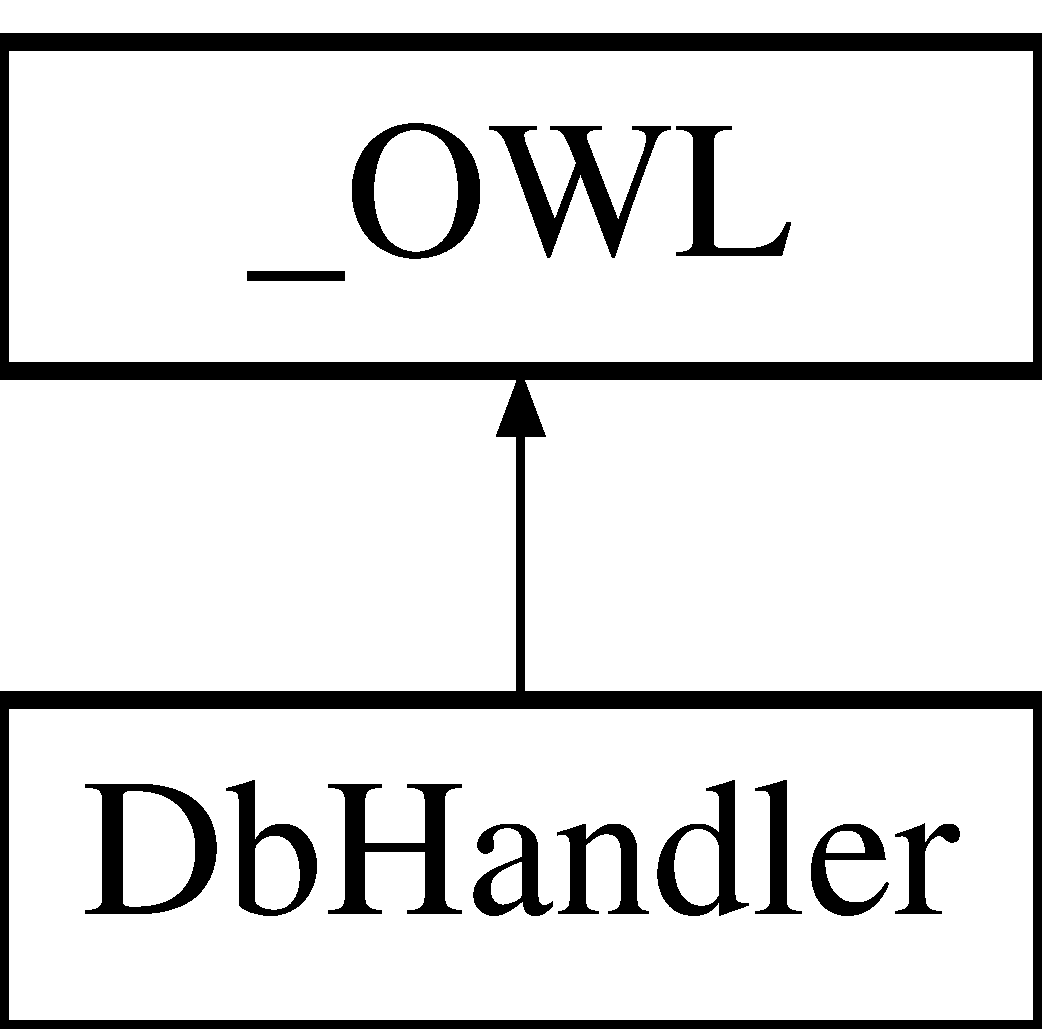
\includegraphics[height=2.000000cm]{classDbHandler}
\end{center}
\end{figure}
\subsection*{Public Member Functions}
\begin{DoxyCompactItemize}
\item 
{\bf \_\-\_\-destruct} ()
\item 
{\bf \_\-\_\-clone} ()
\item 
{\bf alt} (array \$properties)
\item 
{\bf forceReread} ()
\item 
{\bf create} ()
\item 
{\bf isOpen} ()
\item 
{\bf open} ()
\item 
{\bf reset} ()
\item 
{\bf tablename} (\$tablename, \$ignore\_\-backticks=false)
\item 
{\bf setQuery} (\$qry)
\item 
{\bf prepareField} (array \$fielddata)
\item 
{\bf startTransaction} (\$name)
\item 
{\bf commitTransaction} (\$name, \$openNew=false)
\item 
{\bf rollbackTransaction} (\$name, \$openNew=false)
\item 
{\bf resetTable} (\$table)
\item 
{\bf lockTable} (\$tablename, \$locktype)
\item 
{\bf unlockTable} (\$tablename=array())
\item 
{\bf read} (\$flag={\bf DBHANDLE\_\-DATA}, \&\$data, \$quick\_\-query= '', \$line=0, \$file= '[unknown]')
\item 
{\bf tableExists} (\$tablename)
\item 
{\bf escapeString} (\$string)
\item 
{\bf unescapeString} (\$string)
\item 
{\bf prepareRead} (array \$values=array(), array \$tables=array(), array \$searches=array(), array \$joins=array())
\item 
{\bf prepareDelete} (array \$searches=array())
\item 
{\bf prepareUpdate} (array \$values=array(), array \$searches=array(), array \$joins=array())
\item 
{\bf prepareInsert} (array \$values=array())
\item 
{\bf write} (\&\$rows=null, \$line=0, \$file= '[unknown]')
\item 
{\bf lastInsertedId} (\$table=null, \$field=null)
\item 
{\bf close} ()
\item 
{\bf getLastWarning} ()
\item 
{\bf getStatus} ()
\item 
{\bf getSeverity} (\$status=null)
\item 
{\bf succeeded} (\$\_\-ok={\bf OWL\_\-SUCCESS}, \&\$\_\-object=null)
\item 
{\bf signal} (\$level={\bf OWL\_\-INFO}, \&\$text=false)
\item 
{\bf traceback} (\&\$text=false, \$depth=0)
\end{DoxyCompactItemize}
\subsection*{Static Public Member Functions}
\begin{DoxyCompactItemize}
\item 
static {\bf getInstance} ()
\end{DoxyCompactItemize}
\subsection*{Protected Member Functions}
\begin{DoxyCompactItemize}
\item 
{\bf init} ()
\item 
{\bf setCallback} (\$\_\-dispatcher)
\item 
{\bf setCallbackArgument} (array \$\_\-arg)
\item 
{\bf getCallback} ()
\item 
{\bf saveStatus} ()
\item 
{\bf restoreStatus} ()
\item 
{\bf check} (\&\$object, \$level={\bf OWL\_\-WARNING})
\item 
{\bf setStatus} (\$status, \$params=array())
\item 
{\bf setHighSeverity} (\&\$object=null)
\item 
{\bf stackMessage} (\$level={\bf OWL\_\-WARNING})
\end{DoxyCompactItemize}
\subsection*{Protected Attributes}
\begin{DoxyCompactItemize}
\item 
{\bf \$severity}
\end{DoxyCompactItemize}
\subsection*{Private Member Functions}
\begin{DoxyCompactItemize}
\item 
{\bf \_\-\_\-construct} (\$srv= 'localhost', \$db= '', \$usr= '', \$pwd= '', \$dbtype= '{\bf MySQL}')
\item 
{\bf loadDriver} ()
\item 
{\bf connect} ()
\item 
{\bf dbread} (\$qry, \&\$rows, \&\$fields)
\item 
{\bf expandField} (\&\$field, \$check\_\-name=false)
\item 
{\bf tablelist} (array \$tables)
\item 
{\bf whereClause} (array \$searches, array \$joins)
\item 
{\bf updateList} (array \$updates)
\item 
{\bf extractTablelist} (array \$fields)
\item 
{\bf additionalClauses} ()
\end{DoxyCompactItemize}
\subsection*{Private Attributes}
\begin{DoxyCompactItemize}
\item 
{\bf \$id}
\item 
{\bf \$errno}
\item 
{\bf \$error}
\item 
{\bf \$database}
\item 
{\bf \$driver}
\item 
{\bf \$use\_\-backticks}
\item 
{\bf \$rowcount}
\item 
{\bf \$opened}
\item 
{\bf \$db\_\-prefix}
\item 
{\bf \$query}
\item 
{\bf \$ordering}
\item 
{\bf \$grouping}
\item 
{\bf \$having}
\item 
{\bf \$limit}
\item 
{\bf \$query\_\-type}
\item 
{\bf \$transaction}
\item 
{\bf \$locks}
\item 
{\bf \$cloned}
\end{DoxyCompactItemize}
\subsection*{Static Private Attributes}
\begin{DoxyCompactItemize}
\item 
static {\bf \$instance}
\item 
static {\bf \$original\_\-instance}
\end{DoxyCompactItemize}


\subsection{Detailed Description}
Database handler. 

Handler for all database I/O. This singleton class uses an (abstract) class for the actual storage. This class should not be called directly; it is implemented by class \doxyref{DataHandler}{p.}{classDataHandler} \begin{DoxyAuthor}{Author}
Oscar van Eijk, Oveas Functionality Provider 
\end{DoxyAuthor}
\begin{Desc}
\item[{\bf Todo}]Implement retries using the isRetryable() driver method, a max\_\-retries and a max\_\-retry\_\-wait config settings \end{Desc}
\begin{DoxyVersion}{Version}
May 15, 2007 -\/-\/ O van Eijk -\/-\/ initial version for Terra-\/Terra 

Jul 29, 2008 -\/-\/ O van Eijk -\/-\/ Modified version for \doxyref{OWL}{p.}{classOWL} 
\end{DoxyVersion}


\subsection{Constructor \& Destructor Documentation}
\index{DbHandler@{DbHandler}!\_\-\_\-construct@{\_\-\_\-construct}}
\index{\_\-\_\-construct@{\_\-\_\-construct}!DbHandler@{DbHandler}}
\subsubsection[{\_\-\_\-construct}]{\setlength{\rightskip}{0pt plus 5cm}DbHandler::\_\-\_\-construct (
\begin{DoxyParamCaption}
\item[{\$}]{srv = {\ttfamily 'localhost'}, }
\item[{\$}]{db = {\ttfamily ''}, }
\item[{\$}]{usr = {\ttfamily ''}, }
\item[{\$}]{pwd = {\ttfamily ''}, }
\item[{\$}]{dbtype = {\ttfamily '{\bf MySQL}'}}
\end{DoxyParamCaption}
)\hspace{0.3cm}{\ttfamily  [private]}}\label{classDbHandler_ae54e9d4643f41a9296167086f6a769fc}
Class constructor; opens the database connection. 
\begin{DoxyParams}[1]{Parameters}
\mbox{\tt in}  & {\em \$srv} & Database server \\
\hline
\mbox{\tt in}  & {\em \$db} & Database name \\
\hline
\mbox{\tt in}  & {\em \$usr} & Username to connect with \\
\hline
\mbox{\tt in}  & {\em \$pwd} & Password to use for connection \\
\hline
\mbox{\tt in}  & {\em \$dbtype} & Database type, used to load the driver \\
\hline
\end{DoxyParams}
\begin{DoxyAuthor}{Author}
Oscar van Eijk, Oveas Functionality Provider 
\end{DoxyAuthor}


References ConfigHandler::get(), \_\-OWL::init(), loadDriver(), and \_\-OWL::setStatus().

\index{DbHandler@{DbHandler}!\_\-\_\-destruct@{\_\-\_\-destruct}}
\index{\_\-\_\-destruct@{\_\-\_\-destruct}!DbHandler@{DbHandler}}
\subsubsection[{\_\-\_\-destruct}]{\setlength{\rightskip}{0pt plus 5cm}DbHandler::\_\-\_\-destruct (
\begin{DoxyParamCaption}
{}
\end{DoxyParamCaption}
)}\label{classDbHandler_a7cd6bd727d1f296eb5dbfae6ca36ab3f}
Class destructor; closes the database connection \begin{DoxyAuthor}{Author}
Oscar van Eijk, Oveas Functionality Provider 
\end{DoxyAuthor}


Reimplemented from {\bf \_\-OWL} \doxyref{}{p.}{class__OWL_a44fd2222476a3109286cc82d92b6bbcc}.



References close(), commitTransaction(), ConfigHandler::get(), rollbackTransaction(), and unlockTable().



\subsection{Member Function Documentation}
\index{DbHandler@{DbHandler}!\_\-\_\-clone@{\_\-\_\-clone}}
\index{\_\-\_\-clone@{\_\-\_\-clone}!DbHandler@{DbHandler}}
\subsubsection[{\_\-\_\-clone}]{\setlength{\rightskip}{0pt plus 5cm}DbHandler::\_\-\_\-clone (
\begin{DoxyParamCaption}
{}
\end{DoxyParamCaption}
)}\label{classDbHandler_ada20e62b915bc87a1de28389a2ee81e1}
Implementation of the \doxyref{\_\-\_\-clone()}{p.}{classDbHandler_ada20e62b915bc87a1de28389a2ee81e1} function. The current connection will be closed, and a property will be set to indicate this is a cloned object. After that, the \doxyref{alt()}{p.}{classDbHandler_ac3a8e0bfe2491e17bc527715505f90a7} method can be used to change connection info. \begin{DoxyAuthor}{Author}
Oscar van Eijk, Oveas Functionality Provider 
\end{DoxyAuthor}


References \$instance, close(), reset(), and \_\-OWL::setStatus().

\index{DbHandler@{DbHandler}!additionalClauses@{additionalClauses}}
\index{additionalClauses@{additionalClauses}!DbHandler@{DbHandler}}
\subsubsection[{additionalClauses}]{\setlength{\rightskip}{0pt plus 5cm}DbHandler::additionalClauses (
\begin{DoxyParamCaption}
{}
\end{DoxyParamCaption}
)\hspace{0.3cm}{\ttfamily  [private]}}\label{classDbHandler_a9380a7c5c11003d51addd9ea02d41f89}
Check if additional clauses (like GROUP BY, ORDER BY etc) have been defined, and compose this depending on the query type. \begin{DoxyReturn}{Returns}
String with additional clauses 
\end{DoxyReturn}
\begin{DoxyAuthor}{Author}
Oscar van Eijk, Oveas Functionality Provider 
\end{DoxyAuthor}


References expandField().



Referenced by prepareDelete(), prepareInsert(), prepareRead(), and prepareUpdate().

\index{DbHandler@{DbHandler}!alt@{alt}}
\index{alt@{alt}!DbHandler@{DbHandler}}
\subsubsection[{alt}]{\setlength{\rightskip}{0pt plus 5cm}DbHandler::alt (
\begin{DoxyParamCaption}
\item[{array \$}]{properties}
\end{DoxyParamCaption}
)}\label{classDbHandler_ac3a8e0bfe2491e17bc527715505f90a7}
On a cloned database object, set an alternative, prefix or connection. 
\begin{DoxyParams}[1]{Parameters}
\mbox{\tt in}  & {\em \$properties} & An indexed array with the properties that should be changed. Supported are:
\begin{DoxyItemize}
\item prefix : The table prefix
\item server : Database server
\item name : Database name
\item username : Username to connect with
\item password : Password to use for connection
\item dbdriver : Database type (reserved for future use, currently only \doxyref{MySQL}{p.}{classMySQL} is implemented) 
\end{DoxyItemize}\\
\hline
\end{DoxyParams}
\begin{DoxyAuthor}{Author}
Oscar van Eijk, Oveas Functionality Provider 
\end{DoxyAuthor}


References loadDriver(), open(), and \_\-OWL::setStatus().

\index{DbHandler@{DbHandler}!check@{check}}
\index{check@{check}!DbHandler@{DbHandler}}
\subsubsection[{check}]{\setlength{\rightskip}{0pt plus 5cm}\_\-OWL::check (
\begin{DoxyParamCaption}
\item[{\&\$}]{object, }
\item[{\$}]{level = {\ttfamily {\bf OWL\_\-WARNING}}}
\end{DoxyParamCaption}
)\hspace{0.3cm}{\ttfamily  [protected, inherited]}}\label{class__OWL_ae2e3c56e5f3c4ce4156c6b1bb1c50f63}
This is a helper function for lazy developers. Some checks have to be made quite often, this is a kinda macro to handle that. It compares the own severity level with that of a given object. If the highest level is above a given max, a traceback and reset are performed.


\begin{DoxyParams}[1]{Parameters}
\mbox{\tt in}  & {\em \$object} & Pointer to an object to check against \\
\hline
\mbox{\tt in}  & {\em \$level} & The maximum severity level \\
\hline
\end{DoxyParams}
\begin{DoxyReturn}{Returns}
True if the severity level was correct (below the max), otherwise false 
\end{DoxyReturn}
\begin{DoxyAuthor}{Author}
Oscar van Eijk, Oveas Functionality Provider 
\end{DoxyAuthor}


References \_\-OWL::reset(), \_\-OWL::setHighSeverity(), and \_\-OWL::traceback().



Referenced by SessionHandler::write().

\index{DbHandler@{DbHandler}!close@{close}}
\index{close@{close}!DbHandler@{DbHandler}}
\subsubsection[{close}]{\setlength{\rightskip}{0pt plus 5cm}DbHandler::close (
\begin{DoxyParamCaption}
{}
\end{DoxyParamCaption}
)}\label{classDbHandler_ad3d2853bbd2d1962710907e34afb424f}
Close the database and disconnect from the server. This function is called on program shutdown. Although the database will be closed already by PHP, this function might be called at any time manually; is also updates the 'opened' variable. \begin{DoxyAuthor}{Author}
Oscar van Eijk, Oveas Functionality Provider 
\end{DoxyAuthor}


Referenced by \_\-\_\-clone(), \_\-\_\-destruct(), create(), and forceReread().

\index{DbHandler@{DbHandler}!commitTransaction@{commitTransaction}}
\index{commitTransaction@{commitTransaction}!DbHandler@{DbHandler}}
\subsubsection[{commitTransaction}]{\setlength{\rightskip}{0pt plus 5cm}DbHandler::commitTransaction (
\begin{DoxyParamCaption}
\item[{\$}]{name, }
\item[{\$}]{openNew = {\ttfamily false}}
\end{DoxyParamCaption}
)}\label{classDbHandler_ae31ec569a60f730fb1de2ac2b1265338}
Commit database transaction 
\begin{DoxyParams}[1]{Parameters}
\mbox{\tt in}  & {\em \$name} & Transaction name (reserverd for future use) \\
\hline
\mbox{\tt in}  & {\em \$openNew} & Boolean set to true when a new transaction must be opened immediately \\
\hline
\end{DoxyParams}
\begin{DoxyReturn}{Returns}
Object severity status 
\end{DoxyReturn}
\begin{DoxyAuthor}{Author}
Oscar van Eijk, Oveas Functionality Provider 
\end{DoxyAuthor}


References \_\-OWL::setStatus().



Referenced by \_\-\_\-destruct().

\index{DbHandler@{DbHandler}!connect@{connect}}
\index{connect@{connect}!DbHandler@{DbHandler}}
\subsubsection[{connect}]{\setlength{\rightskip}{0pt plus 5cm}DbHandler::connect (
\begin{DoxyParamCaption}
{}
\end{DoxyParamCaption}
)\hspace{0.3cm}{\ttfamily  [private]}}\label{classDbHandler_a9cf52ba614981a0082063d57290d3b7c}
Connect to the database server \begin{DoxyReturn}{Returns}
True on success, otherwise False 
\end{DoxyReturn}
\begin{DoxyAuthor}{Author}
Oscar van Eijk, Oveas Functionality Provider 
\end{DoxyAuthor}


References ConfigHandler::get(), and \_\-OWL::setStatus().



Referenced by create(), and open().

\index{DbHandler@{DbHandler}!create@{create}}
\index{create@{create}!DbHandler@{DbHandler}}
\subsubsection[{create}]{\setlength{\rightskip}{0pt plus 5cm}DbHandler::create (
\begin{DoxyParamCaption}
{}
\end{DoxyParamCaption}
)}\label{classDbHandler_ac9e93cb0ab57f03b2719eebd0c0ee2ef}
Create a new database \begin{DoxyReturn}{Returns}
Severity level 
\end{DoxyReturn}
\begin{DoxyAuthor}{Author}
Oscar van Eijk, Oveas Functionality Provider 
\end{DoxyAuthor}


References close(), connect(), and \_\-OWL::setStatus().

\index{DbHandler@{DbHandler}!dbread@{dbread}}
\index{dbread@{dbread}!DbHandler@{DbHandler}}
\subsubsection[{dbread}]{\setlength{\rightskip}{0pt plus 5cm}DbHandler::dbread (
\begin{DoxyParamCaption}
\item[{\$}]{qry, }
\item[{\&\$}]{rows, }
\item[{\&\$}]{fields}
\end{DoxyParamCaption}
)\hspace{0.3cm}{\ttfamily  [private]}}\label{classDbHandler_a130e49aa639fecb46ce6719ddcb0d72f}
Read from the database. 
\begin{DoxyParams}[1]{Parameters}
\mbox{\tt in}  & {\em \$qry} & Database query string. \\
\hline
\mbox{\tt out}  & {\em \$rows} & Number of rows matched \\
\hline
\mbox{\tt out}  & {\em \$fields} & Number of fields per row \\
\hline
\end{DoxyParams}
\begin{DoxyReturn}{Returns}
A 2D array with all data, or false on failures 
\end{DoxyReturn}
\begin{DoxyAuthor}{Author}
Oscar van Eijk, Oveas Functionality Provider 
\end{DoxyAuthor}


References OWLdbg\_\-add(), and \_\-OWL::setStatus().



Referenced by read().

\index{DbHandler@{DbHandler}!escapeString@{escapeString}}
\index{escapeString@{escapeString}!DbHandler@{DbHandler}}
\subsubsection[{escapeString}]{\setlength{\rightskip}{0pt plus 5cm}DbHandler::escapeString (
\begin{DoxyParamCaption}
\item[{\$}]{string}
\end{DoxyParamCaption}
)}\label{classDbHandler_a84d876a07a292f4a7bd49e5acfac9d14}
Call the current DBtype's escape function for character strings. 
\begin{DoxyParams}{Parameters}
{\em \$string} & The string that should be escaped \\
\hline
\end{DoxyParams}
\begin{DoxyReturn}{Returns}
The escaped string 
\end{DoxyReturn}
\begin{DoxyAuthor}{Author}
Oscar van Eijk, Oveas Functionality Provider 
\end{DoxyAuthor}
\index{DbHandler@{DbHandler}!expandField@{expandField}}
\index{expandField@{expandField}!DbHandler@{DbHandler}}
\subsubsection[{expandField}]{\setlength{\rightskip}{0pt plus 5cm}DbHandler::expandField (
\begin{DoxyParamCaption}
\item[{\&\$}]{field, }
\item[{\$}]{check\_\-name = {\ttfamily false}}
\end{DoxyParamCaption}
)\hspace{0.3cm}{\ttfamily  [private]}}\label{classDbHandler_ad8dac71adf4d540270b5b2c87da114a8}
Change a fieldname in the format 'table\#field' to the format '`[prefix]table.field`' The fieldname can have additional \#-\/seperated elements, which contain the method from the database driver and its arguments (that will be passed as an array) 
\begin{DoxyParams}[1]{Parameters}
\mbox{\tt in,out}  & {\em \$field} & Fieldname to expand \\
\hline
\mbox{\tt in}  & {\em \$check\_\-name} & Boolean which is true if the fieldname should be returned with 'AS'. Default is false \\
\hline
\end{DoxyParams}
\begin{DoxyAuthor}{Author}
Oscar van Eijk, Oveas Functionality Provider 
\end{DoxyAuthor}


References tablename().



Referenced by additionalClauses(), prepareInsert(), prepareRead(), updateList(), and whereClause().

\index{DbHandler@{DbHandler}!extractTablelist@{extractTablelist}}
\index{extractTablelist@{extractTablelist}!DbHandler@{DbHandler}}
\subsubsection[{extractTablelist}]{\setlength{\rightskip}{0pt plus 5cm}DbHandler::extractTablelist (
\begin{DoxyParamCaption}
\item[{array \$}]{fields}
\end{DoxyParamCaption}
)\hspace{0.3cm}{\ttfamily  [private]}}\label{classDbHandler_ab900537e8f8170436f2be39e2a9026cf}
Create an array with unique tablenames as extracted from an array of fields in the format (table::field =$>$ value, ...) 
\begin{DoxyParams}[1]{Parameters}
\mbox{\tt in}  & {\em \$fields} & An array with fields \\
\hline
\end{DoxyParams}
\begin{DoxyReturn}{Returns}
Array with tablenames 
\end{DoxyReturn}
\begin{DoxyAuthor}{Author}
Oscar van Eijk, Oveas Functionality Provider 
\end{DoxyAuthor}


Referenced by prepareDelete(), prepareInsert(), and prepareUpdate().

\index{DbHandler@{DbHandler}!forceReread@{forceReread}}
\index{forceReread@{forceReread}!DbHandler@{DbHandler}}
\subsubsection[{forceReread}]{\setlength{\rightskip}{0pt plus 5cm}DbHandler::forceReread (
\begin{DoxyParamCaption}
{}
\end{DoxyParamCaption}
)}\label{classDbHandler_a1a342f747e4e4c10c00d7d6066d50d59}
Hmmm.... we need this method as the result of a race condition (sort of... I think...); if an alternative database (clone) is opened first, that's the default connection, which is probably the case in most situation since the owl config table is read early in the init phase. I need to think about it... is this solution acceptable? So we need something smarter here? This method is allowed to be called only once by OWLLoader; maybe some checks? \begin{DoxyAuthor}{Author}
Oscar van Eijk, Oveas Functionality Provider 
\end{DoxyAuthor}


References close(), ConfigHandler::get(), loadDriver(), and open().

\index{DbHandler@{DbHandler}!getCallback@{getCallback}}
\index{getCallback@{getCallback}!DbHandler@{DbHandler}}
\subsubsection[{getCallback}]{\setlength{\rightskip}{0pt plus 5cm}\_\-OWL::getCallback (
\begin{DoxyParamCaption}
{}
\end{DoxyParamCaption}
)\hspace{0.3cm}{\ttfamily  [protected, inherited]}}\label{class__OWL_acb46ff88f43ca66f1268d3f5199c3f8d}
Retrieve a previously set (callback) dispatcher. The (callback) dispatcher is cleared immediatly. \begin{DoxyReturn}{Returns}
The dispatcher, of null on failure. 
\end{DoxyReturn}
\begin{DoxyAuthor}{Author}
Oscar van Eijk, Oveas Functionality Provider 
\end{DoxyAuthor}


Reimplemented in {\bf Dispatcher} \doxyref{}{p.}{classDispatcher_a31c4bd4e4eaee7ef90b1ea364a901447}.



References OWL::factory().

\index{DbHandler@{DbHandler}!getInstance@{getInstance}}
\index{getInstance@{getInstance}!DbHandler@{DbHandler}}
\subsubsection[{getInstance}]{\setlength{\rightskip}{0pt plus 5cm}static DbHandler::getInstance (
\begin{DoxyParamCaption}
{}
\end{DoxyParamCaption}
)\hspace{0.3cm}{\ttfamily  [static]}}\label{classDbHandler_a72b64ea1342d97d300d564a7641627d7}
Return a reference to my implementation. If necessary, create that implementation first. \begin{DoxyReturn}{Returns}
Object instance ID 
\end{DoxyReturn}
\begin{DoxyAuthor}{Author}
Oscar van Eijk, Oveas Functionality Provider 
\end{DoxyAuthor}


References \$instance, \$original\_\-instance, and ConfigHandler::get().

\index{DbHandler@{DbHandler}!getLastWarning@{getLastWarning}}
\index{getLastWarning@{getLastWarning}!DbHandler@{DbHandler}}
\subsubsection[{getLastWarning}]{\setlength{\rightskip}{0pt plus 5cm}\_\-OWL::getLastWarning (
\begin{DoxyParamCaption}
{}
\end{DoxyParamCaption}
)\hspace{0.3cm}{\ttfamily  [inherited]}}\label{class__OWL_a1888f52fc2d0ec29e146925ccad70a6b}
Get the last warning or error message. \begin{DoxyReturn}{Returns}
null if there was no error (severity below OWL\_\-WARNING), otherwise the error text. 
\end{DoxyReturn}
\begin{DoxyAuthor}{Author}
Oscar van Eijk, Oveas Functionality Provider 
\end{DoxyAuthor}


References \_\-OWL::signal().

\index{DbHandler@{DbHandler}!getSeverity@{getSeverity}}
\index{getSeverity@{getSeverity}!DbHandler@{DbHandler}}
\subsubsection[{getSeverity}]{\setlength{\rightskip}{0pt plus 5cm}\_\-OWL::getSeverity (
\begin{DoxyParamCaption}
\item[{\$}]{status = {\ttfamily null}}
\end{DoxyParamCaption}
)\hspace{0.3cm}{\ttfamily  [inherited]}}\label{class__OWL_a2374613f9bb7eccf49a5dbc9a9ef4751}
Get the current object severity level. 
\begin{DoxyParams}[1]{Parameters}
\mbox{\tt in}  & {\em \$status} & An optional parameter to check an other status code i.s.o the object's current status. \\
\hline
\end{DoxyParams}
\begin{DoxyReturn}{Returns}
Status severity level 
\end{DoxyReturn}
\begin{DoxyAuthor}{Author}
Oscar van Eijk, Oveas Functionality Provider 
\end{DoxyAuthor}


References \_\-OWL::\$status.



Referenced by LogHandler::composeMessage(), LogHandler::log(), and DataHandler::setKey().

\index{DbHandler@{DbHandler}!getStatus@{getStatus}}
\index{getStatus@{getStatus}!DbHandler@{DbHandler}}
\subsubsection[{getStatus}]{\setlength{\rightskip}{0pt plus 5cm}\_\-OWL::getStatus (
\begin{DoxyParamCaption}
{}
\end{DoxyParamCaption}
)\hspace{0.3cm}{\ttfamily  [final, inherited]}}\label{class__OWL_ac1f1643ff5b5db7c326c30477603358d}
Get the current object status. \begin{DoxyReturn}{Returns}
Object's status code 
\end{DoxyReturn}
\begin{DoxyAuthor}{Author}
Oscar van Eijk, Oveas Functionality Provider 
\end{DoxyAuthor}


Referenced by SchemeHandler::compare().

\index{DbHandler@{DbHandler}!init@{init}}
\index{init@{init}!DbHandler@{DbHandler}}
\subsubsection[{init}]{\setlength{\rightskip}{0pt plus 5cm}\_\-OWL::init (
\begin{DoxyParamCaption}
{}
\end{DoxyParamCaption}
)\hspace{0.3cm}{\ttfamily  [protected, inherited]}}\label{class__OWL_ae0ef3ded56e8a6b34b6461e5a721cd3e}
This function should be called by all constuctors. It initializes the general characteristics. Status is 'warning' by default, it's up to the contructor to set a proper status; if it's still 'warning', this $\ast$might$\ast$ indicate something went wrong. \begin{DoxyAuthor}{Author}
Oscar van Eijk, Oveas Functionality Provider 
\end{DoxyAuthor}


References OWL::factory(), and \_\-OWL::setStatus().



Referenced by FormFieldPlugin::\_\-\_\-construct(), Document::\_\-\_\-construct(), ContainerPlugin::\_\-\_\-construct(), Container::\_\-\_\-construct(), SocketHandler::\_\-\_\-construct(), SessionHandler::\_\-\_\-construct(), SchemeHandler::\_\-\_\-construct(), LogHandler::\_\-\_\-construct(), ImageHandler::\_\-\_\-construct(), FormHandler::\_\-\_\-construct(), FileHandler::\_\-\_\-construct(), \_\-\_\-construct(), HDataHandler::\_\-\_\-construct(), DataHandler::\_\-\_\-construct(), OWL::\_\-\_\-construct(), Mail::\_\-\_\-construct(), Group::\_\-\_\-construct(), Form::\_\-\_\-construct(), Dispatcher::\_\-\_\-construct(), and User::construct().

\index{DbHandler@{DbHandler}!isOpen@{isOpen}}
\index{isOpen@{isOpen}!DbHandler@{DbHandler}}
\subsubsection[{isOpen}]{\setlength{\rightskip}{0pt plus 5cm}DbHandler::isOpen (
\begin{DoxyParamCaption}
{}
\end{DoxyParamCaption}
)}\label{classDbHandler_a71b713d7b974200e64bd606e3b099c38}
Let other objects check if th database connection is opened \begin{DoxyReturn}{Returns}
boolean, True when opened 
\end{DoxyReturn}
\begin{DoxyAuthor}{Author}
Oscar van Eijk, Oveas Functionality Provider 
\end{DoxyAuthor}
\index{DbHandler@{DbHandler}!lastInsertedId@{lastInsertedId}}
\index{lastInsertedId@{lastInsertedId}!DbHandler@{DbHandler}}
\subsubsection[{lastInsertedId}]{\setlength{\rightskip}{0pt plus 5cm}DbHandler::lastInsertedId (
\begin{DoxyParamCaption}
\item[{\$}]{table = {\ttfamily null}, }
\item[{\$}]{field = {\ttfamily null}}
\end{DoxyParamCaption}
)}\label{classDbHandler_a8e1ac478bf6f4e2285d13141fd75bb9e}
Return the last ID after a newly inserted record holding an AUTO\_\-INCREMENT field 
\begin{DoxyParams}[1]{Parameters}
\mbox{\tt in}  & {\em \$table} & Table name holding the auto increment field \\
\hline
\mbox{\tt in}  & {\em \$field} & Name of the auto increment field \\
\hline
\end{DoxyParams}
\begin{DoxyReturn}{Returns}
The number that was last inserted 
\end{DoxyReturn}
\begin{DoxyAuthor}{Author}
Oscar van Eijk, Oveas Functionality Provider 
\end{DoxyAuthor}
\index{DbHandler@{DbHandler}!loadDriver@{loadDriver}}
\index{loadDriver@{loadDriver}!DbHandler@{DbHandler}}
\subsubsection[{loadDriver}]{\setlength{\rightskip}{0pt plus 5cm}DbHandler::loadDriver (
\begin{DoxyParamCaption}
{}
\end{DoxyParamCaption}
)\hspace{0.3cm}{\ttfamily  [private]}}\label{classDbHandler_ab4db7c4fa445700b96a2d4b1be6e50a4}
Create a new instance of the database driver \begin{DoxyAuthor}{Author}
Oscar van Eijk, Oveas Functionality Provider 
\end{DoxyAuthor}


References OWLloader::getDriver(), and toBool().



Referenced by \_\-\_\-construct(), alt(), and forceReread().

\index{DbHandler@{DbHandler}!lockTable@{lockTable}}
\index{lockTable@{lockTable}!DbHandler@{DbHandler}}
\subsubsection[{lockTable}]{\setlength{\rightskip}{0pt plus 5cm}DbHandler::lockTable (
\begin{DoxyParamCaption}
\item[{\$}]{tablename, }
\item[{\$}]{locktype}
\end{DoxyParamCaption}
)}\label{classDbHandler_a27c45a702ae53310ccc159a88bc4234f}
Lock one or more tables 
\begin{DoxyParams}[1]{Parameters}
\mbox{\tt in}  & {\em \$tablename} & Tablename or array of tables \\
\hline
\mbox{\tt in}  & {\em \$locktype} & Locktype as defined in \doxyref{Table lock type}{p.}{group__DBDRIVER__TableLock} \\
\hline
\end{DoxyParams}
\begin{DoxyReturn}{Returns}
Object severity status 
\end{DoxyReturn}
\begin{DoxyAuthor}{Author}
Oscar van Eijk, Oveas Functionality Provider 
\end{DoxyAuthor}
\begin{DoxyNote}{Note}
In \doxyref{MySQL}{p.}{classMySQL}, locks will be released implicetly when a new lock is requested. Also when a new transaction is started, all existing locks are released, so when table locking is required within a transaction, always call \doxyref{lockTable()}{p.}{classDbHandler_a27c45a702ae53310ccc159a88bc4234f} {\itshape after\/} \doxyref{startTransaction()}{p.}{classDbHandler_a19f0cb54f362ab3f919cfc2b940800c0} 
\end{DoxyNote}
\begin{Desc}
\item[{\bf Todo}]This method currenly supports only 1 table and no aliases, must be changed! \end{Desc}


References ConfigHandler::get(), and \_\-OWL::setStatus().

\index{DbHandler@{DbHandler}!open@{open}}
\index{open@{open}!DbHandler@{DbHandler}}
\subsubsection[{open}]{\setlength{\rightskip}{0pt plus 5cm}DbHandler::open (
\begin{DoxyParamCaption}
{}
\end{DoxyParamCaption}
)}\label{classDbHandler_afccbfc69ead84f8445116e050d1cfc2d}
Opens the database connection. \begin{DoxyReturn}{Returns}
Severity level 
\end{DoxyReturn}
\begin{DoxyAuthor}{Author}
Oscar van Eijk, Oveas Functionality Provider 
\end{DoxyAuthor}


References connect(), and \_\-OWL::setStatus().



Referenced by alt(), forceReread(), and read().

\index{DbHandler@{DbHandler}!prepareDelete@{prepareDelete}}
\index{prepareDelete@{prepareDelete}!DbHandler@{DbHandler}}
\subsubsection[{prepareDelete}]{\setlength{\rightskip}{0pt plus 5cm}DbHandler::prepareDelete (
\begin{DoxyParamCaption}
\item[{array \$}]{searches = {\ttfamily array()}}
\end{DoxyParamCaption}
)}\label{classDbHandler_a4dce3c43b43a82a1ac0e3ba2c83309ee}
Prepare a delete query. Data is taken from the arrays that are passed to this function. All fieldnames are in the format 'table\#field', where the table is not yet prefixed. 
\begin{DoxyParams}[1]{Parameters}
\mbox{\tt in}  & {\em \$searches} & Given values that have to match \\
\hline
\end{DoxyParams}
\begin{DoxyReturn}{Returns}
Severity level 
\end{DoxyReturn}
\begin{DoxyAuthor}{Author}
Oscar van Eijk, Oveas Functionality Provider 
\end{DoxyAuthor}


References additionalClauses(), extractTablelist(), OWLdbg\_\-add(), \_\-OWL::setStatus(), tablelist(), and whereClause().

\index{DbHandler@{DbHandler}!prepareField@{prepareField}}
\index{prepareField@{prepareField}!DbHandler@{DbHandler}}
\subsubsection[{prepareField}]{\setlength{\rightskip}{0pt plus 5cm}DbHandler::prepareField (
\begin{DoxyParamCaption}
\item[{array \$}]{fielddata}
\end{DoxyParamCaption}
)}\label{classDbHandler_aab87f0d23357d708c7f327e3875366ad}
Prepare a field for use in the upconimg query using the array as set by DbHandler::set(). Internal arrays are filled with grouping data, ordering data etc. if required., 
\begin{DoxyParams}[1]{Parameters}
\mbox{\tt in}  & {\em \$fielddata} & Array with a description of the field, \\
\hline
\end{DoxyParams}
\begin{DoxySeeAlso}{See also}
DbHandler::set() 
\end{DoxySeeAlso}
\begin{DoxyReturn}{Returns}
An array with two elements: the fieldname in the format that will be handled by \doxyref{DbHandler::expandField()}{p.}{classDbHandler_ad8dac71adf4d540270b5b2c87da114a8}, and the value which might be a normal value, an array of values of a value as set by a driver function (using database functions). On errors, null is returned. 
\end{DoxyReturn}
\begin{DoxyAuthor}{Author}
Oscar van Eijk, Oveas Functionality Provider 
\end{DoxyAuthor}


References \_\-OWL::setStatus().

\index{DbHandler@{DbHandler}!prepareInsert@{prepareInsert}}
\index{prepareInsert@{prepareInsert}!DbHandler@{DbHandler}}
\subsubsection[{prepareInsert}]{\setlength{\rightskip}{0pt plus 5cm}DbHandler::prepareInsert (
\begin{DoxyParamCaption}
\item[{array \$}]{values = {\ttfamily array()}}
\end{DoxyParamCaption}
)}\label{classDbHandler_a50f426084a888714b72bedb42de7ebc4}
Prepare an insert query. Data is taken from the arrays that are passed to this function. All fieldnames are in the format 'table\#field', where the table is not yet prefixed. 
\begin{DoxyParams}[1]{Parameters}
\mbox{\tt in}  & {\em \$values} & Given database values \\
\hline
\end{DoxyParams}
\begin{DoxyReturn}{Returns}
Severity level 
\end{DoxyReturn}
\begin{DoxyAuthor}{Author}
Oscar van Eijk, Oveas Functionality Provider 
\end{DoxyAuthor}


References additionalClauses(), expandField(), extractTablelist(), OWLdbg\_\-add(), \_\-OWL::setStatus(), and tablename().

\index{DbHandler@{DbHandler}!prepareRead@{prepareRead}}
\index{prepareRead@{prepareRead}!DbHandler@{DbHandler}}
\subsubsection[{prepareRead}]{\setlength{\rightskip}{0pt plus 5cm}DbHandler::prepareRead (
\begin{DoxyParamCaption}
\item[{array \$}]{values = {\ttfamily array()}, }
\item[{array \$}]{tables = {\ttfamily array()}, }
\item[{array \$}]{searches = {\ttfamily array()}, }
\item[{array \$}]{joins = {\ttfamily array()}}
\end{DoxyParamCaption}
)}\label{classDbHandler_a2f749a426fa9dbfe1b58a7d0d4263d1f}
Prepare a read query. Data is taken from the arrays that are passed to this function. All fieldnames are in the format 'table\#field', where the table is not yet prefixed. 
\begin{DoxyParams}[1]{Parameters}
\mbox{\tt in}  & {\em \$values} & Values that will be read \\
\hline
\mbox{\tt in}  & {\em \$tables} & Tables from which will be read \\
\hline
\mbox{\tt in}  & {\em \$searches} & Given values that have to match \\
\hline
\mbox{\tt in}  & {\em \$joins} & Joins on the given tables \\
\hline
\end{DoxyParams}
\begin{DoxyReturn}{Returns}
Severity level 
\end{DoxyReturn}
\begin{DoxyAuthor}{Author}
Oscar van Eijk, Oveas Functionality Provider 
\end{DoxyAuthor}


References additionalClauses(), expandField(), OWLdbg\_\-add(), \_\-OWL::setStatus(), tablelist(), and whereClause().

\index{DbHandler@{DbHandler}!prepareUpdate@{prepareUpdate}}
\index{prepareUpdate@{prepareUpdate}!DbHandler@{DbHandler}}
\subsubsection[{prepareUpdate}]{\setlength{\rightskip}{0pt plus 5cm}DbHandler::prepareUpdate (
\begin{DoxyParamCaption}
\item[{array \$}]{values = {\ttfamily array()}, }
\item[{array \$}]{searches = {\ttfamily array()}, }
\item[{array \$}]{joins = {\ttfamily array()}}
\end{DoxyParamCaption}
)}\label{classDbHandler_abe6db4c3099ca5cfcfb75e9eb34ba2af}
Prepare an update query. Data is taken from the arrays that are passed to this function. All fieldnames are in the format 'table\#field', where the table is not yet prefixed. 
\begin{DoxyParams}[1]{Parameters}
\mbox{\tt in}  & {\em \$values} & Given database values \\
\hline
\mbox{\tt in}  & {\em \$searches} & List of fieldnames that will be used in the where clause. All fields not in this array will be updated! \\
\hline
\mbox{\tt in}  & {\em \$joins} & Joins on the given tables \\
\hline
\end{DoxyParams}
\begin{DoxyReturn}{Returns}
Severity level 
\end{DoxyReturn}
\begin{DoxyAuthor}{Author}
Oscar van Eijk, Oveas Functionality Provider 
\end{DoxyAuthor}


References additionalClauses(), extractTablelist(), OWLdbg\_\-add(), \_\-OWL::setStatus(), tablelist(), updateList(), and whereClause().

\index{DbHandler@{DbHandler}!read@{read}}
\index{read@{read}!DbHandler@{DbHandler}}
\subsubsection[{read}]{\setlength{\rightskip}{0pt plus 5cm}DbHandler::read (
\begin{DoxyParamCaption}
\item[{\$}]{flag = {\ttfamily {\bf DBHANDLE\_\-DATA}}, }
\item[{\&\$}]{data, }
\item[{\$}]{quick\_\-query = {\ttfamily ''}, }
\item[{\$}]{line = {\ttfamily 0}, }
\item[{\$}]{file = {\ttfamily '[unknown]'}}
\end{DoxyParamCaption}
)}\label{classDbHandler_a5ebfdc2acfcb0e9cbc2861fc55c7127c}
Read from the database. The return value depends on the flag. By default, the selected rows(s) are returned in a 2d array. 
\begin{DoxyParams}[1]{Parameters}
\mbox{\tt in}  & {\em \$flag} & Flag that identifies how data should be returned; as data (default) or the number of rows \\
\hline
\mbox{\tt out}  & {\em \$data} & The retrieved value in a format depending on the flag:
\begin{DoxyItemize}
\item DBHANDLE\_\-ROWCOUNT; Number of matching rows
\item DBHANDLE\_\-FIELDCOUNT; Number of fields per rows
\item DBHANDLE\_\-TOTALFIELDCOUNT; Total number op fields
\item DBHANDLE\_\-DATA (default); A 2D array with all data
\item DBHANDLE\_\-SINGLEROW; The first matching row in a 1D array
\item DBHANDLE\_\-SINGLEFIELD; The first matching field 
\end{DoxyItemize}\\
\hline
\mbox{\tt in}  & {\em \$quick\_\-query} & Database query string. If empty, \$this-\/$>$query is used \\
\hline
\mbox{\tt in}  & {\em \$line} & Line number of this call \\
\hline
\mbox{\tt in}  & {\em \$file} & File that made the call to this method \\
\hline
\end{DoxyParams}
\begin{DoxyReturn}{Returns}
Severity level 
\end{DoxyReturn}
\begin{DoxyAuthor}{Author}
Oscar van Eijk, Oveas Functionality Provider 
\end{DoxyAuthor}


References dbread(), open(), and \_\-OWL::setStatus().

\index{DbHandler@{DbHandler}!reset@{reset}}
\index{reset@{reset}!DbHandler@{DbHandler}}
\subsubsection[{reset}]{\setlength{\rightskip}{0pt plus 5cm}DbHandler::reset (
\begin{DoxyParamCaption}
{}
\end{DoxyParamCaption}
)}\label{classDbHandler_a9982df4830f05803935bb31bac7fae3d}
Reset the object \begin{DoxyAuthor}{Author}
Oscar van Eijk, Oveas Functionality Provider 
\end{DoxyAuthor}


Reimplemented from {\bf \_\-OWL} \doxyref{}{p.}{class__OWL_a2f2a042bcf31965194c03033df0edc9b}.



Referenced by \_\-\_\-clone().

\index{DbHandler@{DbHandler}!resetTable@{resetTable}}
\index{resetTable@{resetTable}!DbHandler@{DbHandler}}
\subsubsection[{resetTable}]{\setlength{\rightskip}{0pt plus 5cm}DbHandler::resetTable (
\begin{DoxyParamCaption}
\item[{\$}]{table}
\end{DoxyParamCaption}
)}\label{classDbHandler_abbef28b434626bedd9d16d85526adde8}
Erase the full contents of a table and reset counters if applicable 
\begin{DoxyParams}[1]{Parameters}
\mbox{\tt in}  & {\em \$table} & Table name \\
\hline
\end{DoxyParams}
\begin{DoxyReturn}{Returns}
Objects severity level 
\end{DoxyReturn}
\begin{DoxyAuthor}{Author}
Oscar van Eijk, Oveas Functionality Provider 
\end{DoxyAuthor}


References \_\-OWL::setStatus().

\index{DbHandler@{DbHandler}!restoreStatus@{restoreStatus}}
\index{restoreStatus@{restoreStatus}!DbHandler@{DbHandler}}
\subsubsection[{restoreStatus}]{\setlength{\rightskip}{0pt plus 5cm}\_\-OWL::restoreStatus (
\begin{DoxyParamCaption}
{}
\end{DoxyParamCaption}
)\hspace{0.3cm}{\ttfamily  [protected, inherited]}}\label{class__OWL_a93de01a9bbbc3f228e1a62a0740e90f0}
Restore the previously saved status object and destroy the copy \begin{DoxyAuthor}{Author}
Oscar van Eijk, Oveas Functionality Provider 
\end{DoxyAuthor}


References \_\-OWL::setStatus().



Referenced by User::logout().

\index{DbHandler@{DbHandler}!rollbackTransaction@{rollbackTransaction}}
\index{rollbackTransaction@{rollbackTransaction}!DbHandler@{DbHandler}}
\subsubsection[{rollbackTransaction}]{\setlength{\rightskip}{0pt plus 5cm}DbHandler::rollbackTransaction (
\begin{DoxyParamCaption}
\item[{\$}]{name, }
\item[{\$}]{openNew = {\ttfamily false}}
\end{DoxyParamCaption}
)}\label{classDbHandler_ad62c686d350ee350849ea42687492a48}
Rollback the current transaction 
\begin{DoxyParams}[1]{Parameters}
\mbox{\tt in}  & {\em \$name} & Transaction name (reserverd for future use) \\
\hline
\mbox{\tt in}  & {\em \$openNew} & Boolean set to true when a new transaction must be opened immediately \\
\hline
\end{DoxyParams}
\begin{DoxyReturn}{Returns}
Object severity status 
\end{DoxyReturn}
\begin{DoxyAuthor}{Author}
Oscar van Eijk, Oveas Functionality Provider 
\end{DoxyAuthor}


References \_\-OWL::setStatus().



Referenced by \_\-\_\-destruct().

\index{DbHandler@{DbHandler}!saveStatus@{saveStatus}}
\index{saveStatus@{saveStatus}!DbHandler@{DbHandler}}
\subsubsection[{saveStatus}]{\setlength{\rightskip}{0pt plus 5cm}\_\-OWL::saveStatus (
\begin{DoxyParamCaption}
{}
\end{DoxyParamCaption}
)\hspace{0.3cm}{\ttfamily  [protected, inherited]}}\label{class__OWL_add923dc756471318edca8883db3f4420}
Create a copy of the status object \begin{DoxyAuthor}{Author}
Oscar van Eijk, Oveas Functionality Provider 
\end{DoxyAuthor}


Referenced by User::logout().

\index{DbHandler@{DbHandler}!setCallback@{setCallback}}
\index{setCallback@{setCallback}!DbHandler@{DbHandler}}
\subsubsection[{setCallback}]{\setlength{\rightskip}{0pt plus 5cm}\_\-OWL::setCallback (
\begin{DoxyParamCaption}
\item[{\$}]{\_\-dispatcher}
\end{DoxyParamCaption}
)\hspace{0.3cm}{\ttfamily  [protected, inherited]}}\label{class__OWL_a5f84d43cd4dc7810649f1e2ebecad360}
Set a dispatcher for later callback 
\begin{DoxyParams}[1]{Parameters}
\mbox{\tt in}  & {\em \$\_\-dispatcher} & Dispatched, \\
\hline
\end{DoxyParams}
\begin{DoxySeeAlso}{See also}
\doxyref{Dispatcher::composeDispatcher()}{p.}{classDispatcher_a8a974bbbb30be7cda74f9929972fd2f6} 
\end{DoxySeeAlso}
\begin{DoxyReturn}{Returns}
True on success, false on failure 
\end{DoxyReturn}
\begin{DoxyAuthor}{Author}
Oscar van Eijk, Oveas Functionality Provider 
\end{DoxyAuthor}


References OWL::factory().

\index{DbHandler@{DbHandler}!setCallbackArgument@{setCallbackArgument}}
\index{setCallbackArgument@{setCallbackArgument}!DbHandler@{DbHandler}}
\subsubsection[{setCallbackArgument}]{\setlength{\rightskip}{0pt plus 5cm}\_\-OWL::setCallbackArgument (
\begin{DoxyParamCaption}
\item[{array \$}]{\_\-arg}
\end{DoxyParamCaption}
)\hspace{0.3cm}{\ttfamily  [protected, inherited]}}\label{class__OWL_a4e9ebfbd3c0d76539bed4e44de9962c3}
Add an argument to a previously registered callback dispatcher 
\begin{DoxyParams}[1]{Parameters}
\mbox{\tt in}  & {\em \$\_\-arg} & Argument, must be an array type. When non-\/ arrays should be passed as arguments, the must be set when the callback is registered already \\
\hline
\end{DoxyParams}
\begin{DoxyReturn}{Returns}
True on success, false on failure 
\end{DoxyReturn}
\begin{DoxyAuthor}{Author}
Oscar van Eijk, Oveas Functionality Provider 
\end{DoxyAuthor}


References OWL::factory().



Referenced by User::register().

\index{DbHandler@{DbHandler}!setHighSeverity@{setHighSeverity}}
\index{setHighSeverity@{setHighSeverity}!DbHandler@{DbHandler}}
\subsubsection[{setHighSeverity}]{\setlength{\rightskip}{0pt plus 5cm}\_\-OWL::setHighSeverity (
\begin{DoxyParamCaption}
\item[{\&\$}]{object = {\ttfamily null}}
\end{DoxyParamCaption}
)\hspace{0.3cm}{\ttfamily  [protected, inherited]}}\label{class__OWL_a97173dbe452428d3851406413264734d}
Compare the severity level of the current object with a given one and set my statuspointer to the object with the highest level. \begin{DoxyAuthor}{Author}
Oscar van Eijk, Oveas Functionality Provider 
\end{DoxyAuthor}


Referenced by \_\-OWL::check(), DataHandler::db(), DataHandler::prepare(), and SessionHandler::read().

\index{DbHandler@{DbHandler}!setQuery@{setQuery}}
\index{setQuery@{setQuery}!DbHandler@{DbHandler}}
\subsubsection[{setQuery}]{\setlength{\rightskip}{0pt plus 5cm}DbHandler::setQuery (
\begin{DoxyParamCaption}
\item[{\$}]{qry}
\end{DoxyParamCaption}
)}\label{classDbHandler_a14787a81542efc8dea40060532e5ddca}
Set the database query. This function should only be used if the query is too complex to be set with any of the prepare() functions. 
\begin{DoxyParams}[1]{Parameters}
\mbox{\tt in}  & {\em \$qry} & A complete database query. All tablenames must be prefixed (with the \doxyref{tablename()}{p.}{classDbHandler_a05ea485a22c0ef87090f2313614c84c8} function)! \\
\hline
\end{DoxyParams}
\begin{DoxyAuthor}{Author}
Oscar van Eijk, Oveas Functionality Provider 
\end{DoxyAuthor}
\index{DbHandler@{DbHandler}!setStatus@{setStatus}}
\index{setStatus@{setStatus}!DbHandler@{DbHandler}}
\subsubsection[{setStatus}]{\setlength{\rightskip}{0pt plus 5cm}\_\-OWL::setStatus (
\begin{DoxyParamCaption}
\item[{\$}]{status, }
\item[{\$}]{params = {\ttfamily array~()}}
\end{DoxyParamCaption}
)\hspace{0.3cm}{\ttfamily  [final, protected, inherited]}}\label{class__OWL_a80e2fe01c3663dbb0ab685eebe33fd1e}
Set the current object status to the specified value. 
\begin{DoxyParams}[1]{Parameters}
\mbox{\tt in}  & {\em \$status} & \doxyref{OWL}{p.}{classOWL} status code \\
\hline
\mbox{\tt in}  & {\em \$params} & \\
\hline
\end{DoxyParams}
\begin{DoxyAuthor}{Author}
Oscar van Eijk, Oveas Functionality Provider 
\end{DoxyAuthor}


References \$GLOBALS, \_\-OWL::\$status, ConfigHandler::get(), Register::getCode(), \_\-OWL::reset(), and \_\-OWL::signal().



Referenced by \_\-\_\-clone(), Container::\_\-\_\-construct(), SocketHandler::\_\-\_\-construct(), SchemeHandler::\_\-\_\-construct(), ImageHandler::\_\-\_\-construct(), FormHandler::\_\-\_\-construct(), FileHandler::\_\-\_\-construct(), \_\-\_\-construct(), DataHandler::\_\-\_\-construct(), Session::\_\-\_\-construct(), Mail::\_\-\_\-construct(), BaseElement::\_\-getContent(), HDataHandler::\_\-getNewLeft(), Mail::addBcc(), Mail::addCc(), Container::addContainer(), Form::addField(), FormFieldRadioPlugin::addOption(), HDataHandler::addParent(), Mail::addTo(), BaseElement::addToContent(), alt(), SchemeHandler::alterScheme(), FileHandler::close(), commitTransaction(), Dispatcher::composeDispatcher(), User::confirm(), SocketHandler::connect(), connect(), create(), SchemeHandler::createScheme(), dbread(), SchemeHandler::defineIndex(), SchemeHandler::defineScheme(), SocketHandler::disconnect(), Dispatcher::dispatch(), HDataHandler::enableCrossLink(), FormHandler::get(), DataHandler::get(), HDataHandler::getDirectChildren(), HDataHandler::getFullOffspring(), Group::getGroupByName(), SchemeHandler::getTableColumns(), SchemeHandler::getTableIndexes(), \_\-OWL::init(), Document::loadScript(), Document::loadStyle(), lockTable(), User::login(), HDataHandler::moveNode(), FileHandler::open(), open(), LogHandler::openLogfile(), DataHandler::prepare(), prepareDelete(), prepareField(), prepareInsert(), prepareRead(), prepareUpdate(), SocketHandler::read(), read(), FileHandler::readLine(), HDataHandler::readQuery(), User::readUserdata(), User::register(), Dispatcher::registerArgument(), Dispatcher::registerCallback(), resetTable(), \_\-OWL::restoreStatus(), rollbackTransaction(), SchemeHandler::scheme(), Mail::send(), FormHandler::set(), BaseElement::setAttributes(), BaseElement::setContent(), Form::setEncoding(), Document::setFavicon(), Form::setFieldAttributes(), Mail::setFrom(), DataHandler::setJoin(), DataHandler::setKey(), FormFieldTextPlugin::setMaxsize(), Document::setMeta(), Form::setMethod(), FormFieldRadioPlugin::setSelected(), Mail::setSender(), FormFieldTextPlugin::setSize(), FormFieldSelectPlugin::setSize(), FormFieldSelectPlugin::setValue(), Form::showField(), startTransaction(), SchemeHandler::tableDescription(), unlockTable(), SchemeHandler::validateScheme(), SocketHandler::write(), write(), and HDataHandler::writeQuery().

\index{DbHandler@{DbHandler}!signal@{signal}}
\index{signal@{signal}!DbHandler@{DbHandler}}
\subsubsection[{signal}]{\setlength{\rightskip}{0pt plus 5cm}\_\-OWL::signal (
\begin{DoxyParamCaption}
\item[{\$}]{level = {\ttfamily {\bf OWL\_\-INFO}}, }
\item[{\&\$}]{text = {\ttfamily false}}
\end{DoxyParamCaption}
)\hspace{0.3cm}{\ttfamily  [inherited]}}\label{class__OWL_a51ba4a16409acf2a2f61f286939091a5}
Display the message for the current object status 
\begin{DoxyParams}[1]{Parameters}
\mbox{\tt in}  & {\em \$level} & An optional severity level; message will only be displayed when it is at least of this level. \\
\hline
\mbox{\tt out}  & {\em \$text} & If this parameter is given, the message text is returned in this string instead of echood. \\
\hline
\end{DoxyParams}
\begin{DoxyReturn}{Returns}
The severity level for this object 
\end{DoxyReturn}
\begin{DoxyAuthor}{Author}
Oscar van Eijk, Oveas Functionality Provider 
\end{DoxyAuthor}


References ConfigHandler::get(), OutputHandler::outputLine(), and OutputHandler::outputRaw().



Referenced by \_\-OWL::getLastWarning(), \_\-OWL::setStatus(), \_\-OWL::stackMessage(), and \_\-OWL::traceback().

\index{DbHandler@{DbHandler}!stackMessage@{stackMessage}}
\index{stackMessage@{stackMessage}!DbHandler@{DbHandler}}
\subsubsection[{stackMessage}]{\setlength{\rightskip}{0pt plus 5cm}\_\-OWL::stackMessage (
\begin{DoxyParamCaption}
\item[{\$}]{level = {\ttfamily {\bf OWL\_\-WARNING}}}
\end{DoxyParamCaption}
)\hspace{0.3cm}{\ttfamily  [protected, inherited]}}\label{class__OWL_acbb85f4949ca4bbd8bb2408362632cbc}
Add the message for the latests status change to the document \begin{DoxySeeAlso}{See also}
\doxyref{Document::addMessage()}{p.}{classDocument_aee4ecb0f14972dafd3114659b57048b3} 
\end{DoxySeeAlso}

\begin{DoxyParams}[1]{Parameters}
\mbox{\tt in}  & {\em \$level} & Minimum severity level \\
\hline
\end{DoxyParams}
\begin{DoxyAuthor}{Author}
Oscar van Eijk, Oveas Functionality Provider 
\end{DoxyAuthor}


References \$\_\-doc, \_\-OWL::\$severity, OWL::factory(), and \_\-OWL::signal().

\index{DbHandler@{DbHandler}!startTransaction@{startTransaction}}
\index{startTransaction@{startTransaction}!DbHandler@{DbHandler}}
\subsubsection[{startTransaction}]{\setlength{\rightskip}{0pt plus 5cm}DbHandler::startTransaction (
\begin{DoxyParamCaption}
\item[{\$}]{name}
\end{DoxyParamCaption}
)}\label{classDbHandler_a19f0cb54f362ab3f919cfc2b940800c0}
Start a new database transaction 
\begin{DoxyParams}[1]{Parameters}
\mbox{\tt in}  & {\em \$name} & Transaction name (reserverd for future use) \\
\hline
\end{DoxyParams}
\begin{DoxyReturn}{Returns}
Object severity status 
\end{DoxyReturn}
\begin{DoxyAuthor}{Author}
Oscar van Eijk, Oveas Functionality Provider 
\end{DoxyAuthor}


References \_\-OWL::setStatus().

\index{DbHandler@{DbHandler}!succeeded@{succeeded}}
\index{succeeded@{succeeded}!DbHandler@{DbHandler}}
\subsubsection[{succeeded}]{\setlength{\rightskip}{0pt plus 5cm}\_\-OWL::succeeded (
\begin{DoxyParamCaption}
\item[{\$}]{\_\-ok = {\ttfamily {\bf OWL\_\-SUCCESS}}, }
\item[{\&\$}]{\_\-object = {\ttfamily null}}
\end{DoxyParamCaption}
)\hspace{0.3cm}{\ttfamily  [inherited]}}\label{class__OWL_a53ab4d3bbb2c6a56966c339ca4b4c805}
Check if the object currenlty has a success state 
\begin{DoxyParams}[1]{Parameters}
\mbox{\tt in}  & {\em \$\_\-ok} & The highest severity that's considered successfull, default OWL\_\-SUCCESS \\
\hline
\mbox{\tt in}  & {\em \$\_\-object} & REference to the object to check, defaults to the current object \\
\hline
\end{DoxyParams}
\begin{DoxyReturn}{Returns}
Boolean true when successfull 
\end{DoxyReturn}
\begin{DoxyAuthor}{Author}
Oscar van Eijk, Oveas Functionality Provider 
\end{DoxyAuthor}


Referenced by User::construct(), Dispatcher::registerArgument(), and Dispatcher::registerCallback().

\index{DbHandler@{DbHandler}!tableExists@{tableExists}}
\index{tableExists@{tableExists}!DbHandler@{DbHandler}}
\subsubsection[{tableExists}]{\setlength{\rightskip}{0pt plus 5cm}DbHandler::tableExists (
\begin{DoxyParamCaption}
\item[{\$}]{tablename}
\end{DoxyParamCaption}
)}\label{classDbHandler_a139d99b594ab5b95da378d7b281ae8a0}
Check if a table exists in the database 
\begin{DoxyParams}[1]{Parameters}
\mbox{\tt in}  & {\em \$tablename} & Name of the table to check \\
\hline
\end{DoxyParams}
\begin{DoxyReturn}{Returns}
True of the table exists 
\end{DoxyReturn}
\begin{DoxyAuthor}{Author}
Oscar van Eijk, Oveas Functionality Provider 
\end{DoxyAuthor}


References tablename().

\index{DbHandler@{DbHandler}!tablelist@{tablelist}}
\index{tablelist@{tablelist}!DbHandler@{DbHandler}}
\subsubsection[{tablelist}]{\setlength{\rightskip}{0pt plus 5cm}DbHandler::tablelist (
\begin{DoxyParamCaption}
\item[{array \$}]{tables}
\end{DoxyParamCaption}
)\hspace{0.3cm}{\ttfamily  [private]}}\label{classDbHandler_a0ea7d40a222cf6f1bf77b42e8eba03e4}
Create a list with tables, including prefixes, that can be interpreted by SQL 
\begin{DoxyParams}[1]{Parameters}
\mbox{\tt in}  & {\em \$tables} & An array with tablenames \\
\hline
\end{DoxyParams}
\begin{DoxyReturn}{Returns}
The tablelist 
\end{DoxyReturn}
\begin{DoxyAuthor}{Author}
Oscar van Eijk, Oveas Functionality Provider 
\end{DoxyAuthor}


References tablename().



Referenced by prepareDelete(), prepareRead(), and prepareUpdate().

\index{DbHandler@{DbHandler}!tablename@{tablename}}
\index{tablename@{tablename}!DbHandler@{DbHandler}}
\subsubsection[{tablename}]{\setlength{\rightskip}{0pt plus 5cm}DbHandler::tablename (
\begin{DoxyParamCaption}
\item[{\$}]{tablename, }
\item[{\$}]{ignore\_\-backticks = {\ttfamily false}}
\end{DoxyParamCaption}
)}\label{classDbHandler_a05ea485a22c0ef87090f2313614c84c8}
Extend a tablename with the database prefix 
\begin{DoxyParams}[1]{Parameters}
\mbox{\tt in}  & {\em \$tablename} & Table name to extend \\
\hline
\mbox{\tt in}  & {\em \$ignore\_\-backticks} & Boolean to suppress backticks if set, default false \\
\hline
\end{DoxyParams}
\begin{DoxyReturn}{Returns}
Extended table name 
\end{DoxyReturn}
\begin{DoxyAuthor}{Author}
Oscar van Eijk, Oveas Functionality Provider 
\end{DoxyAuthor}


Referenced by expandField(), prepareInsert(), tableExists(), and tablelist().

\index{DbHandler@{DbHandler}!traceback@{traceback}}
\index{traceback@{traceback}!DbHandler@{DbHandler}}
\subsubsection[{traceback}]{\setlength{\rightskip}{0pt plus 5cm}\_\-OWL::traceback (
\begin{DoxyParamCaption}
\item[{\&\$}]{text = {\ttfamily false}, }
\item[{\$}]{depth = {\ttfamily 0}}
\end{DoxyParamCaption}
)\hspace{0.3cm}{\ttfamily  [inherited]}}\label{class__OWL_aa29547995d6741b7d2b90c1d4ea99a13}
If somehwere in the nested calls an error occured, we can traceback the original failing object with this function and signal the message. 
\begin{DoxyParams}[1]{Parameters}
\mbox{\tt out}  & {\em \$text} & Optional variable in which the message text can be stored. If not given, the text will be written to standard output \\
\hline
\mbox{\tt in}  & {\em \$depth} & This paramater should be initially empty. It calculates the depth in recursive calls. \\
\hline
\end{DoxyParams}
\begin{DoxyReturn}{Returns}
Severity code of the failing object 
\end{DoxyReturn}
\begin{DoxyAuthor}{Author}
Oscar van Eijk, Oveas Functionality Provider 
\end{DoxyAuthor}


References \_\-OWL::signal().



Referenced by \_\-OWL::check(), User::login(), and SessionHandler::read().

\index{DbHandler@{DbHandler}!unescapeString@{unescapeString}}
\index{unescapeString@{unescapeString}!DbHandler@{DbHandler}}
\subsubsection[{unescapeString}]{\setlength{\rightskip}{0pt plus 5cm}DbHandler::unescapeString (
\begin{DoxyParamCaption}
\item[{\$}]{string}
\end{DoxyParamCaption}
)}\label{classDbHandler_a03b7dab122b64aa5653dffb3e7150271}
Call the current DBtype's unescape function for character strings. 
\begin{DoxyParams}{Parameters}
{\em \$string} & The string that should be unescaped \\
\hline
\end{DoxyParams}
\begin{DoxyReturn}{Returns}
The unescaped string 
\end{DoxyReturn}
\begin{DoxyAuthor}{Author}
Oscar van Eijk, Oveas Functionality Provider 
\end{DoxyAuthor}
\index{DbHandler@{DbHandler}!unlockTable@{unlockTable}}
\index{unlockTable@{unlockTable}!DbHandler@{DbHandler}}
\subsubsection[{unlockTable}]{\setlength{\rightskip}{0pt plus 5cm}DbHandler::unlockTable (
\begin{DoxyParamCaption}
\item[{\$}]{tablename = {\ttfamily array()}}
\end{DoxyParamCaption}
)}\label{classDbHandler_a09617f79a9c3b699f0237cd682a97d96}
Unlock one or more tables 
\begin{DoxyParams}[1]{Parameters}
\mbox{\tt in}  & {\em \$tablename} & Tablename or array of tables. An empty array (default) results in releaseing all current locks \\
\hline
\end{DoxyParams}
\begin{DoxyReturn}{Returns}
Object severity status 
\end{DoxyReturn}
\begin{DoxyAuthor}{Author}
Oscar van Eijk, Oveas Functionality Provider 
\end{DoxyAuthor}


References ConfigHandler::get(), and \_\-OWL::setStatus().



Referenced by \_\-\_\-destruct().

\index{DbHandler@{DbHandler}!updateList@{updateList}}
\index{updateList@{updateList}!DbHandler@{DbHandler}}
\subsubsection[{updateList}]{\setlength{\rightskip}{0pt plus 5cm}DbHandler::updateList (
\begin{DoxyParamCaption}
\item[{array \$}]{updates}
\end{DoxyParamCaption}
)\hspace{0.3cm}{\ttfamily  [private]}}\label{classDbHandler_a1340ca63d23565b97218846e77272410}
Create a string with 'field = value, ...' combinations in SQL format 
\begin{DoxyParams}[1]{Parameters}
\mbox{\tt in}  & {\em \$updates} & Array with fields to update (fieldname =$>$ values) \\
\hline
\end{DoxyParams}
\begin{DoxyReturn}{Returns}
The UPDATE statement 
\end{DoxyReturn}
\begin{DoxyAuthor}{Author}
Oscar van Eijk, Oveas Functionality Provider 
\end{DoxyAuthor}


References expandField().



Referenced by prepareUpdate().

\index{DbHandler@{DbHandler}!whereClause@{whereClause}}
\index{whereClause@{whereClause}!DbHandler@{DbHandler}}
\subsubsection[{whereClause}]{\setlength{\rightskip}{0pt plus 5cm}DbHandler::whereClause (
\begin{DoxyParamCaption}
\item[{array \$}]{searches, }
\item[{array \$}]{joins}
\end{DoxyParamCaption}
)\hspace{0.3cm}{\ttfamily  [private]}}\label{classDbHandler_a4458733bab22e5487f700f7107a4e091}
Create a WHERE clause that can be interpreted by SQL 
\begin{DoxyParams}[1]{Parameters}
\mbox{\tt in}  & {\em \$searches} & Array with values (fieldname =$>$ values) Values can be an array in which case more ORs for that field will be added to the where clause \\
\hline
\mbox{\tt in}  & {\em \$joins} & Array of arrays with values (field, linktype, field) \\
\hline
\end{DoxyParams}
\begin{DoxyReturn}{Returns}
The WHERE clause 
\end{DoxyReturn}
\begin{DoxyAuthor}{Author}
Oscar van Eijk, Oveas Functionality Provider 
\end{DoxyAuthor}


References expandField().



Referenced by prepareDelete(), prepareRead(), and prepareUpdate().

\index{DbHandler@{DbHandler}!write@{write}}
\index{write@{write}!DbHandler@{DbHandler}}
\subsubsection[{write}]{\setlength{\rightskip}{0pt plus 5cm}DbHandler::write (
\begin{DoxyParamCaption}
\item[{\&\$}]{rows = {\ttfamily null}, }
\item[{\$}]{line = {\ttfamily 0}, }
\item[{\$}]{file = {\ttfamily '[unknown]'}}
\end{DoxyParamCaption}
)}\label{classDbHandler_ac02a117c76d5d20ec950fcd5aae9cf8d}
Database inserts and updates. The number of affected rows is stored in \$this-\/$>$rowcount 
\begin{DoxyParams}[1]{Parameters}
\mbox{\tt out}  & {\em \$rows} & (optional) The number of affected rows \\
\hline
\mbox{\tt in}  & {\em \$line} & Line number of this call \\
\hline
\mbox{\tt in}  & {\em \$file} & File that made the call to this method \\
\hline
\end{DoxyParams}
\begin{DoxyReturn}{Returns}
Severity level 
\end{DoxyReturn}
\begin{DoxyAuthor}{Author}
Oscar van Eijk, Oveas Functionality Provider 
\end{DoxyAuthor}


References \_\-OWL::setStatus().



\subsection{Member Data Documentation}
\index{DbHandler@{DbHandler}!\$cloned@{\$cloned}}
\index{\$cloned@{\$cloned}!DbHandler@{DbHandler}}
\subsubsection[{\$cloned}]{\setlength{\rightskip}{0pt plus 5cm}DbHandler::\$cloned\hspace{0.3cm}{\ttfamily  [private]}}\label{classDbHandler_a6fc74f6785f349ab442f33ce31f46e63}
boolean -\/ true when the object has been cloned \index{DbHandler@{DbHandler}!\$database@{\$database}}
\index{\$database@{\$database}!DbHandler@{DbHandler}}
\subsubsection[{\$database}]{\setlength{\rightskip}{0pt plus 5cm}DbHandler::\$database\hspace{0.3cm}{\ttfamily  [private]}}\label{classDbHandler_afaac5248f9ee59786b48a7b51f318940}
array -\/ Database location and authorization indo \index{DbHandler@{DbHandler}!\$db\_\-prefix@{\$db\_\-prefix}}
\index{\$db\_\-prefix@{\$db\_\-prefix}!DbHandler@{DbHandler}}
\subsubsection[{\$db\_\-prefix}]{\setlength{\rightskip}{0pt plus 5cm}DbHandler::\$db\_\-prefix\hspace{0.3cm}{\ttfamily  [private]}}\label{classDbHandler_a19af96598e7f72673fc5da26ad77731b}
string -\/ database prefix \index{DbHandler@{DbHandler}!\$driver@{\$driver}}
\index{\$driver@{\$driver}!DbHandler@{DbHandler}}
\subsubsection[{\$driver}]{\setlength{\rightskip}{0pt plus 5cm}DbHandler::\$driver\hspace{0.3cm}{\ttfamily  [private]}}\label{classDbHandler_a7fa6c2e54682982813e963fd738d1a1b}
object -\/ The database driver \index{DbHandler@{DbHandler}!\$errno@{\$errno}}
\index{\$errno@{\$errno}!DbHandler@{DbHandler}}
\subsubsection[{\$errno}]{\setlength{\rightskip}{0pt plus 5cm}DbHandler::\$errno\hspace{0.3cm}{\ttfamily  [private]}}\label{classDbHandler_af6e9f493be56617cb533763bb2a0e85a}
integer -\/ Error ID \index{DbHandler@{DbHandler}!\$error@{\$error}}
\index{\$error@{\$error}!DbHandler@{DbHandler}}
\subsubsection[{\$error}]{\setlength{\rightskip}{0pt plus 5cm}DbHandler::\$error\hspace{0.3cm}{\ttfamily  [private]}}\label{classDbHandler_ade79e11156abbfc180864beb5b9df377}
string -\/ Error text \index{DbHandler@{DbHandler}!\$grouping@{\$grouping}}
\index{\$grouping@{\$grouping}!DbHandler@{DbHandler}}
\subsubsection[{\$grouping}]{\setlength{\rightskip}{0pt plus 5cm}DbHandler::\$grouping\hspace{0.3cm}{\ttfamily  [private]}}\label{classDbHandler_a8491f7d8d0e7c1d87ba40eb084bee17c}
array -\/ list of fields for a GROUP BY clause \index{DbHandler@{DbHandler}!\$having@{\$having}}
\index{\$having@{\$having}!DbHandler@{DbHandler}}
\subsubsection[{\$having}]{\setlength{\rightskip}{0pt plus 5cm}DbHandler::\$having\hspace{0.3cm}{\ttfamily  [private]}}\label{classDbHandler_aa547d4ff326eafb6b128820f4284ede4}
array -\/ list of fields for a HAVING clause \index{DbHandler@{DbHandler}!\$id@{\$id}}
\index{\$id@{\$id}!DbHandler@{DbHandler}}
\subsubsection[{\$id}]{\setlength{\rightskip}{0pt plus 5cm}DbHandler::\$id\hspace{0.3cm}{\ttfamily  [private]}}\label{classDbHandler_ad38e1c3312815c8ad4093957881092ff}
integer -\/ DB Handle ID \index{DbHandler@{DbHandler}!\$instance@{\$instance}}
\index{\$instance@{\$instance}!DbHandler@{DbHandler}}
\subsubsection[{\$instance}]{\setlength{\rightskip}{0pt plus 5cm}DbHandler::\$instance\hspace{0.3cm}{\ttfamily  [static, private]}}\label{classDbHandler_a0859a862eac3e8ba14c6d04de0396710}
integer -\/ self reference 

Referenced by \_\-\_\-clone(), and getInstance().

\index{DbHandler@{DbHandler}!\$limit@{\$limit}}
\index{\$limit@{\$limit}!DbHandler@{DbHandler}}
\subsubsection[{\$limit}]{\setlength{\rightskip}{0pt plus 5cm}DbHandler::\$limit\hspace{0.3cm}{\ttfamily  [private]}}\label{classDbHandler_a3a05faa4d14c6c5117ed8b70fc37d778}
array with 2 elements to limit the query \begin{Desc}
\item[{\bf Todo}]this ain't implemented yet \end{Desc}
\index{DbHandler@{DbHandler}!\$locks@{\$locks}}
\index{\$locks@{\$locks}!DbHandler@{DbHandler}}
\subsubsection[{\$locks}]{\setlength{\rightskip}{0pt plus 5cm}DbHandler::\$locks\hspace{0.3cm}{\ttfamily  [private]}}\label{classDbHandler_a05f47a3d47e57349f05dec8c8a88b0c2}
array -\/ list of tables that are currently locked \index{DbHandler@{DbHandler}!\$opened@{\$opened}}
\index{\$opened@{\$opened}!DbHandler@{DbHandler}}
\subsubsection[{\$opened}]{\setlength{\rightskip}{0pt plus 5cm}DbHandler::\$opened\hspace{0.3cm}{\ttfamily  [private]}}\label{classDbHandler_a71e36ffbff0d157b1d91dc000bc6f821}
boolean -\/ True if the database is opened \index{DbHandler@{DbHandler}!\$ordering@{\$ordering}}
\index{\$ordering@{\$ordering}!DbHandler@{DbHandler}}
\subsubsection[{\$ordering}]{\setlength{\rightskip}{0pt plus 5cm}DbHandler::\$ordering\hspace{0.3cm}{\ttfamily  [private]}}\label{classDbHandler_a385a4c0af492f9c5db699d0b854cf88c}
array -\/ list of fields for an ORDER BY clasue \index{DbHandler@{DbHandler}!\$original\_\-instance@{\$original\_\-instance}}
\index{\$original\_\-instance@{\$original\_\-instance}!DbHandler@{DbHandler}}
\subsubsection[{\$original\_\-instance}]{\setlength{\rightskip}{0pt plus 5cm}DbHandler::\$original\_\-instance\hspace{0.3cm}{\ttfamily  [static, private]}}\label{classDbHandler_a495ca4030e7ca7d5e8c7e2604e042dfe}
integer -\/ self reference to the original object before cloning 

Referenced by getInstance().

\index{DbHandler@{DbHandler}!\$query@{\$query}}
\index{\$query@{\$query}!DbHandler@{DbHandler}}
\subsubsection[{\$query}]{\setlength{\rightskip}{0pt plus 5cm}DbHandler::\$query\hspace{0.3cm}{\ttfamily  [private]}}\label{classDbHandler_ad671b5596b37dac6d48a660a07775965}
string -\/ Query string \index{DbHandler@{DbHandler}!\$query\_\-type@{\$query\_\-type}}
\index{\$query\_\-type@{\$query\_\-type}!DbHandler@{DbHandler}}
\subsubsection[{\$query\_\-type}]{\setlength{\rightskip}{0pt plus 5cm}DbHandler::\$query\_\-type\hspace{0.3cm}{\ttfamily  [private]}}\label{classDbHandler_afba491ae1a1f1b9343cb65c87ef1e2a9}
string -\/ Prepared query type \index{DbHandler@{DbHandler}!\$rowcount@{\$rowcount}}
\index{\$rowcount@{\$rowcount}!DbHandler@{DbHandler}}
\subsubsection[{\$rowcount}]{\setlength{\rightskip}{0pt plus 5cm}DbHandler::\$rowcount\hspace{0.3cm}{\ttfamily  [private]}}\label{classDbHandler_a56a7ae4bd7d842c85f3fe8052aecbfef}
integer -\/ Row counter \index{DbHandler@{DbHandler}!\$severity@{\$severity}}
\index{\$severity@{\$severity}!DbHandler@{DbHandler}}
\subsubsection[{\$severity}]{\setlength{\rightskip}{0pt plus 5cm}\_\-OWL::\$severity\hspace{0.3cm}{\ttfamily  [protected, inherited]}}\label{class__OWL_ad26b40a9dbbacb33e299b17826f8327c}
Severity level of the current object status 

Referenced by \_\-OWL::stackMessage().

\index{DbHandler@{DbHandler}!\$transaction@{\$transaction}}
\index{\$transaction@{\$transaction}!DbHandler@{DbHandler}}
\subsubsection[{\$transaction}]{\setlength{\rightskip}{0pt plus 5cm}DbHandler::\$transaction\hspace{0.3cm}{\ttfamily  [private]}}\label{classDbHandler_a4b95a0aa4fbae5d63d6f960984a276af}
string -\/ name of the open transaction (currently just used as a boolean) \index{DbHandler@{DbHandler}!\$use\_\-backticks@{\$use\_\-backticks}}
\index{\$use\_\-backticks@{\$use\_\-backticks}!DbHandler@{DbHandler}}
\subsubsection[{\$use\_\-backticks}]{\setlength{\rightskip}{0pt plus 5cm}DbHandler::\$use\_\-backticks\hspace{0.3cm}{\ttfamily  [private]}}\label{classDbHandler_aba13a0ae78c5665670778ed51be722d3}
boolean -\/ true when Backticks should be used in the queries, this can be defined in the driver using the constant USE\_\-BACKTICKS. Default is false 

The documentation for this class was generated from the following file:\begin{DoxyCompactItemize}
\item 
/home/oscar/projects/owl-\/php/src/kernel/so/{\bf class.dbhandler.php}\end{DoxyCompactItemize}

\section{Dispatcher Class Reference}
\label{classDispatcher}\index{Dispatcher@{Dispatcher}}


\hyperlink{classDispatcher}{Dispatcher} singleton.  




Inheritance diagram for Dispatcher:
\nopagebreak
\begin{figure}[H]
\begin{center}
\leavevmode
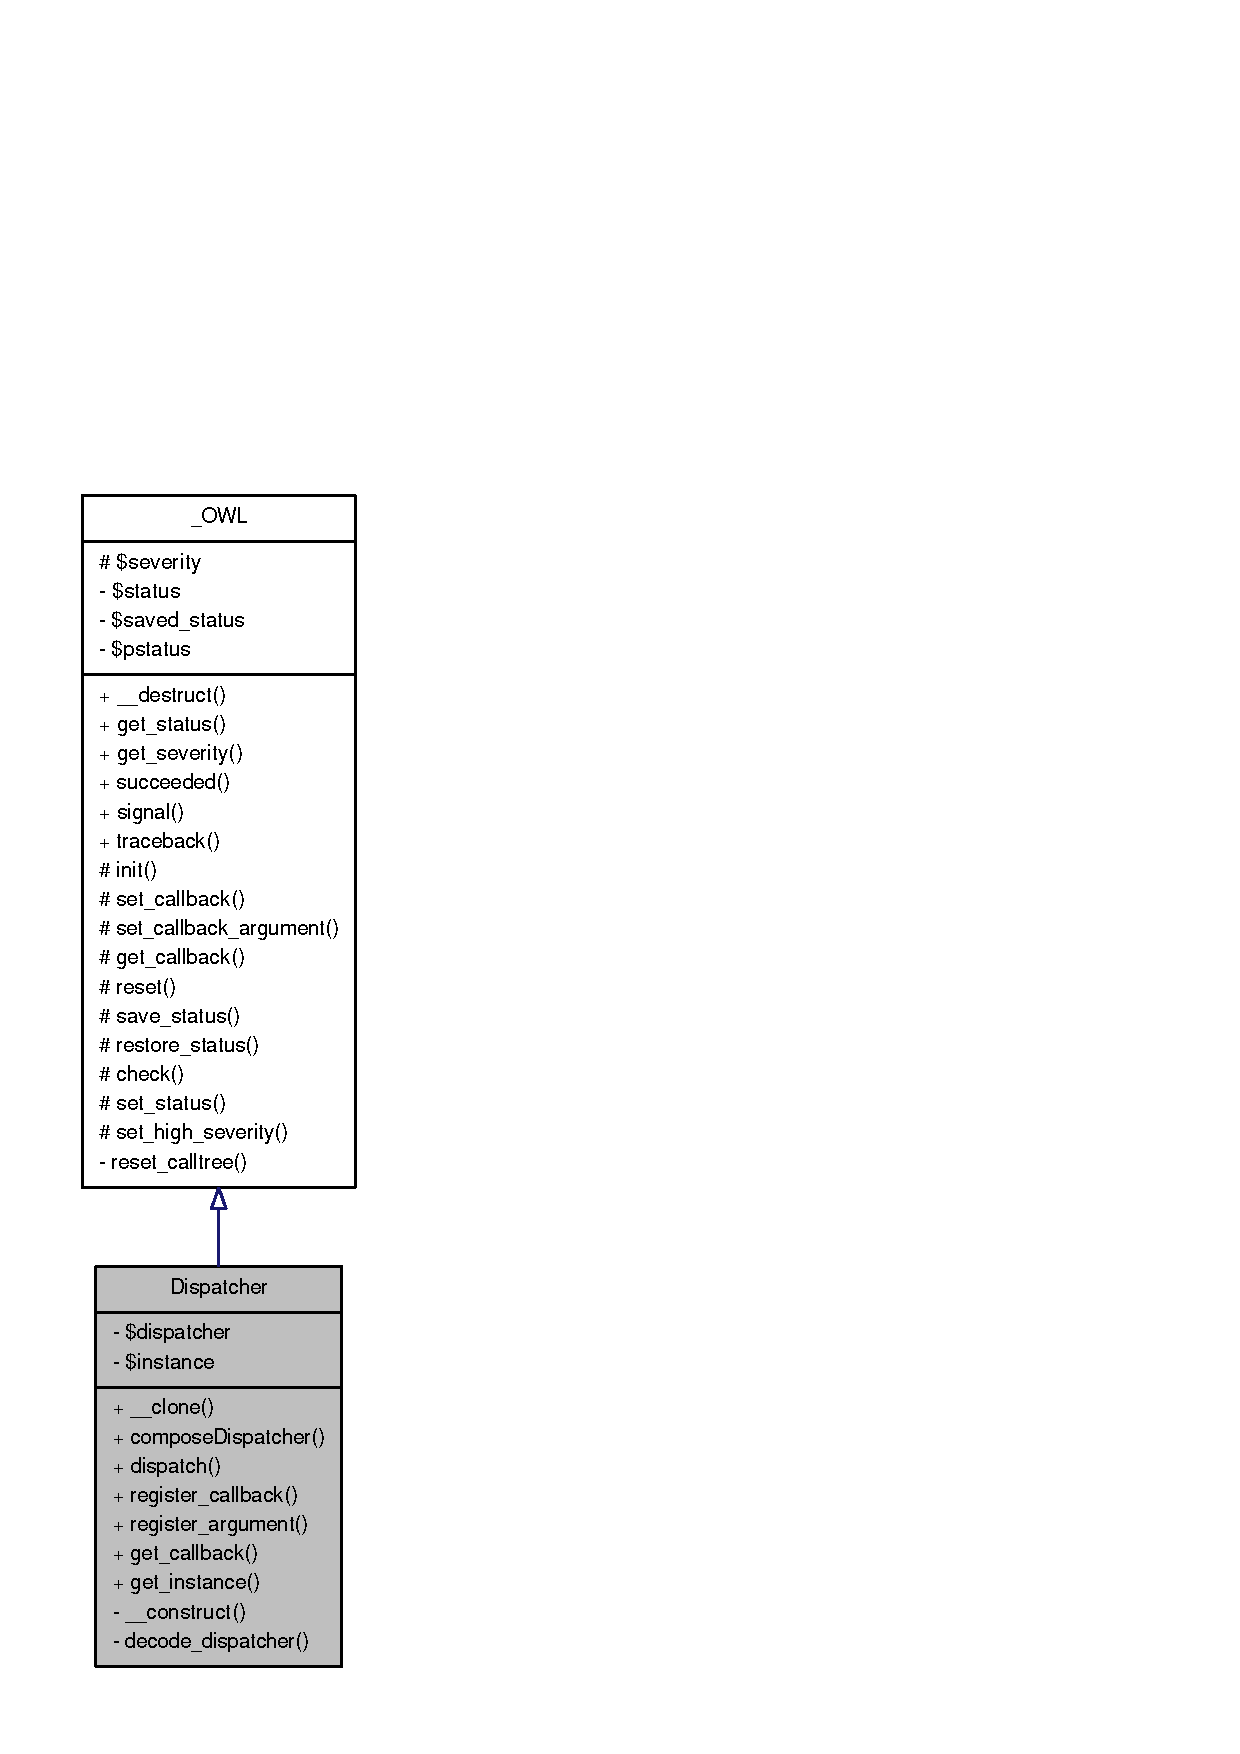
\includegraphics[width=162pt]{classDispatcher__inherit__graph}
\end{center}
\end{figure}


Collaboration diagram for Dispatcher:
\nopagebreak
\begin{figure}[H]
\begin{center}
\leavevmode
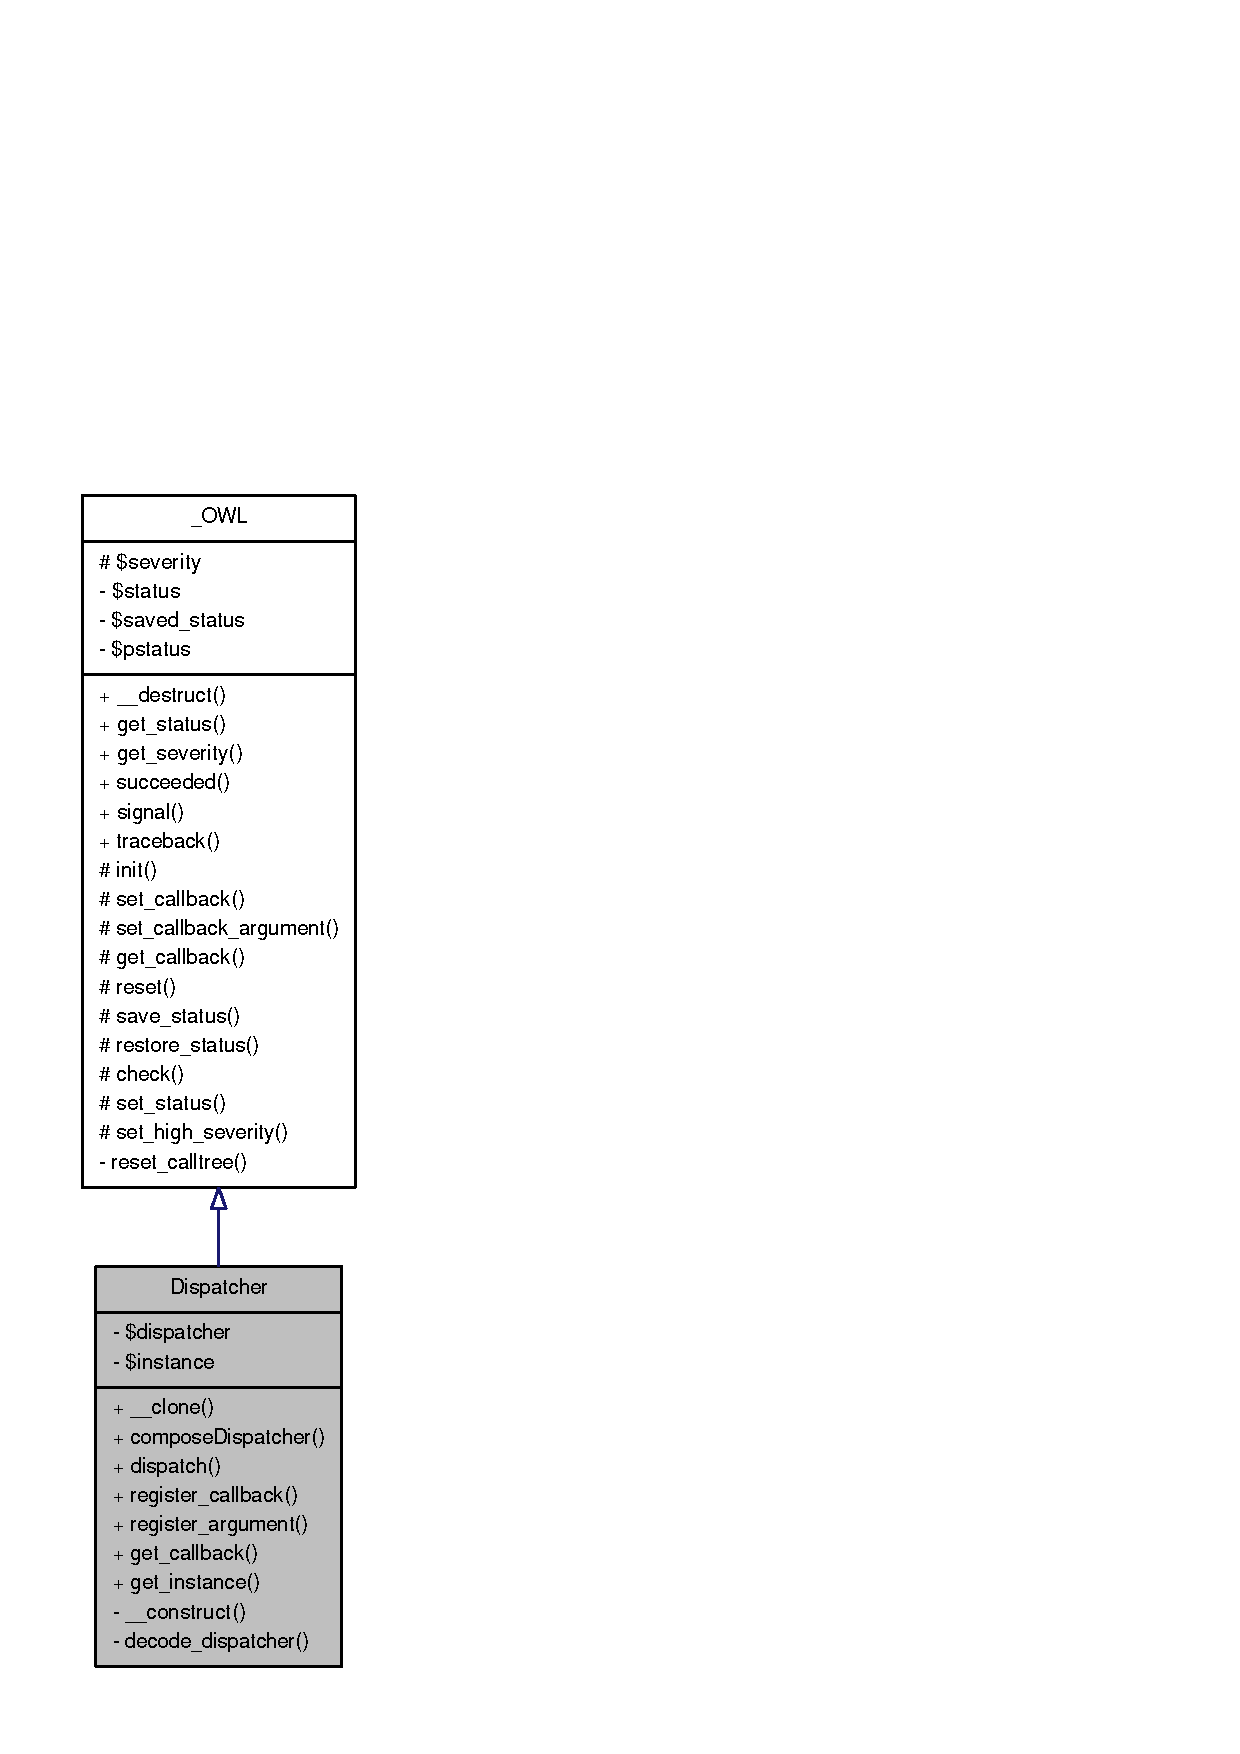
\includegraphics[width=162pt]{classDispatcher__coll__graph}
\end{center}
\end{figure}
\subsection*{Public Member Functions}
\begin{DoxyCompactItemize}
\item 
\hyperlink{classDispatcher_a601d9fd6c9a2ccbfd77b43b6f7678ba3}{\_\-\_\-clone} ()
\item 
\hyperlink{classDispatcher_a8a974bbbb30be7cda74f9929972fd2f6}{composeDispatcher} (\$\_\-dispatcher)
\item 
\hyperlink{classDispatcher_a55f3a6e89f797e2986d32166cfa49486}{dispatch} (\$\_\-dispatcher=null)
\item 
\hyperlink{class__OWL_a99ec771fa2c5c279f80152cc09e489a8}{get\_\-status} ()
\item 
\hyperlink{class__OWL_adf9509ef96858be7bdd9414c5ef129aa}{get\_\-severity} (\$status=null)
\item 
\hyperlink{class__OWL_a51ba4a16409acf2a2f61f286939091a5}{signal} (\$level=\hyperlink{owl_8severitycodes_8php_a139328861128689f2f4def6a399d9057}{OWL\_\-INFO}, \&\$text=false)
\item 
\hyperlink{class__OWL_aa29547995d6741b7d2b90c1d4ea99a13}{traceback} (\&\$text=false, \$depth=0)
\end{DoxyCompactItemize}
\subsection*{Static Public Member Functions}
\begin{DoxyCompactItemize}
\item 
static \hyperlink{classDispatcher_af9998a41bc9dec229b58924e9d5e5e6a}{get\_\-instance} ()
\end{DoxyCompactItemize}
\subsection*{Protected Member Functions}
\begin{DoxyCompactItemize}
\item 
\hyperlink{class__OWL_ae0ef3ded56e8a6b34b6461e5a721cd3e}{init} ()
\item 
\hyperlink{class__OWL_a2f2a042bcf31965194c03033df0edc9b}{reset} ()
\item 
\hyperlink{class__OWL_a9e49b9c76fbc021b244c6915ea536d71}{save\_\-status} ()
\item 
\hyperlink{class__OWL_a465eeaf40edd9f9c848841700c32ce55}{restore\_\-status} ()
\item 
\hyperlink{class__OWL_ad6f4f6946f40199dd0333cf219fa500e}{check} (\&\$object, \$level)
\item 
\hyperlink{class__OWL_aea912d0ede9b3c2a69b79072d94d4787}{set\_\-status} (\$status, \$params=array())
\item 
\hyperlink{class__OWL_a576829692a3b66e3d518853bf43abae3}{set\_\-high\_\-severity} (\&\$object=null)
\end{DoxyCompactItemize}
\subsection*{Protected Attributes}
\begin{DoxyCompactItemize}
\item 
\hyperlink{class__OWL_ad26b40a9dbbacb33e299b17826f8327c}{\$severity}
\end{DoxyCompactItemize}
\subsection*{Private Member Functions}
\begin{DoxyCompactItemize}
\item 
\hyperlink{classDispatcher_a62ba56a9c99d2b25616023812d965c32}{\_\-\_\-construct} ()
\end{DoxyCompactItemize}
\subsection*{Static Private Attributes}
\begin{DoxyCompactItemize}
\item 
static \hyperlink{classDispatcher_a676b77546f23eb5bae93d28362664eb8}{\$instance}
\end{DoxyCompactItemize}


\subsection{Detailed Description}
\hyperlink{classDispatcher}{Dispatcher} singleton. Define the dispatcher. This class calls the proper method based in the request or form data \begin{DoxyAuthor}{Author}
Oscar van Eijk, Oveas Functionality Provider 
\end{DoxyAuthor}
\begin{DoxyVersion}{Version}
Nov 23, 2010 -\/-\/ O van Eijk -\/-\/ initial version 
\end{DoxyVersion}


\subsection{Constructor \& Destructor Documentation}
\index{Dispatcher@{Dispatcher}!\_\-\_\-construct@{\_\-\_\-construct}}
\index{\_\-\_\-construct@{\_\-\_\-construct}!Dispatcher@{Dispatcher}}
\subsubsection[{\_\-\_\-construct}]{\setlength{\rightskip}{0pt plus 5cm}Dispatcher::\_\-\_\-construct (
\begin{DoxyParamCaption}
{}
\end{DoxyParamCaption}
)\hspace{0.3cm}{\ttfamily  \mbox{[}private\mbox{]}}}\label{classDispatcher_a62ba56a9c99d2b25616023812d965c32}
Constructor 

References \_\-OWL::init().



\subsection{Member Function Documentation}
\index{Dispatcher@{Dispatcher}!\_\-\_\-clone@{\_\-\_\-clone}}
\index{\_\-\_\-clone@{\_\-\_\-clone}!Dispatcher@{Dispatcher}}
\subsubsection[{\_\-\_\-clone}]{\setlength{\rightskip}{0pt plus 5cm}Dispatcher::\_\-\_\-clone (
\begin{DoxyParamCaption}
{}
\end{DoxyParamCaption}
)}\label{classDispatcher_a601d9fd6c9a2ccbfd77b43b6f7678ba3}
Implementation of the \hyperlink{classDispatcher_a601d9fd6c9a2ccbfd77b43b6f7678ba3}{\_\-\_\-clone()} function to prevent cloning of this singleton; it triggers a fatal (user)error \index{Dispatcher@{Dispatcher}!check@{check}}
\index{check@{check}!Dispatcher@{Dispatcher}}
\subsubsection[{check}]{\setlength{\rightskip}{0pt plus 5cm}\_\-OWL::check (
\begin{DoxyParamCaption}
\item[{\&\$}]{ object, }
\item[{\$}]{ level}
\end{DoxyParamCaption}
)\hspace{0.3cm}{\ttfamily  \mbox{[}protected, inherited\mbox{]}}}\label{class__OWL_ad6f4f6946f40199dd0333cf219fa500e}
This is a helper function for lazy developers. Some checks have to be made quite often, this is a kinda macro to handle that. It compares the own severity level with that of a given object. If the highest level is above a given max, a traceback and reset are performed.


\begin{DoxyParams}{Parameters}
\item[\mbox{\tt[in]} {\em \$object}]Pointer to an object to check against \item[\mbox{\tt[in]} {\em \$level}]The maximum severity level \end{DoxyParams}
\begin{DoxyReturn}{Returns}
True if the severity level was correct ( below the max), otherwise false 
\end{DoxyReturn}


References \_\-OWL::reset(), \_\-OWL::set\_\-high\_\-severity(), and \_\-OWL::traceback().



Referenced by SessionHandler::write().

\index{Dispatcher@{Dispatcher}!composeDispatcher@{composeDispatcher}}
\index{composeDispatcher@{composeDispatcher}!Dispatcher@{Dispatcher}}
\subsubsection[{composeDispatcher}]{\setlength{\rightskip}{0pt plus 5cm}Dispatcher::composeDispatcher (
\begin{DoxyParamCaption}
\item[{\$}]{ \_\-dispatcher}
\end{DoxyParamCaption}
)}\label{classDispatcher_a8a974bbbb30be7cda74f9929972fd2f6}
Translate a given dispatcher to the URL encoded format 
\begin{DoxyParams}{Parameters}
\item[\mbox{\tt[in]} {\em \$\_\-dispatcher}]\hyperlink{classDispatcher}{Dispatcher} as an indexed array with the following keys:
\begin{DoxyItemize}
\item application: Name of the application. When the include path is no constant, it must be equal to the name of the directory directly under the server's document root.
\item include\_\-path: A path relative from the application toplevel, or a constant
\item class\_\-file: Filename, this can be the full file name (\char`\"{}class.myclass.php\char`\"{}) or just the name (\char`\"{}myclass\char`\"{})
\item class\_\-name Name of the class. This can be ommitted if it is equal to the classfile starting with a capital (\char`\"{}Myclass\char`\"{})
\item method\_\-name: Methpd that will be called when the form is submitted. This method should accept no parameters, but must get the formdata using \hyperlink{classOWL_aa6f4f99b9b0d6c77e7d49075d8a29d69}{OWL::factory}('FormHandler'); For short, a string in the format \char`\"{}application\#include\_\-path-\/path\#class\_\-file\#class\_\-name\#method\_\-name\char`\"{} may also be given. 
\end{DoxyItemize}\end{DoxyParams}
\begin{DoxyReturn}{Returns}
URL encoded dispatcher 
\end{DoxyReturn}


References owlCrypt(), and \_\-OWL::set\_\-status().

\index{Dispatcher@{Dispatcher}!dispatch@{dispatch}}
\index{dispatch@{dispatch}!Dispatcher@{Dispatcher}}
\subsubsection[{dispatch}]{\setlength{\rightskip}{0pt plus 5cm}Dispatcher::dispatch (
\begin{DoxyParamCaption}
\item[{\$}]{ \_\-dispatcher = {\ttfamily null}}
\end{DoxyParamCaption}
)}\label{classDispatcher_a55f3a6e89f797e2986d32166cfa49486}
Get the dispatcher info from the formdata, load the specified classfile and call the method specified. 
\begin{DoxyParams}{Parameters}
\item[\mbox{\tt[in]} {\em \$\_\-dispatcher}]An optional dispatcher can be given (\end{DoxyParams}
\begin{DoxySeeAlso}{See also}
\hyperlink{classDispatcher_a8a974bbbb30be7cda74f9929972fd2f6}{Dispatcher::composeDispatcher()} for the format). When omitted, the dispatcher will be taken from the formdata.
\end{DoxySeeAlso}
\begin{DoxyReturn}{Returns}
On errors during dispatch, the severity level, otherwise the return value of the given method 
\end{DoxyReturn}


References \$\_\-form, OWL::factory(), OWLloader::getClass(), owlCrypt(), and \_\-OWL::set\_\-status().

\index{Dispatcher@{Dispatcher}!get\_\-instance@{get\_\-instance}}
\index{get\_\-instance@{get\_\-instance}!Dispatcher@{Dispatcher}}
\subsubsection[{get\_\-instance}]{\setlength{\rightskip}{0pt plus 5cm}static Dispatcher::get\_\-instance (
\begin{DoxyParamCaption}
{}
\end{DoxyParamCaption}
)\hspace{0.3cm}{\ttfamily  \mbox{[}static\mbox{]}}}\label{classDispatcher_af9998a41bc9dec229b58924e9d5e5e6a}
Return a reference to my implementation. If necessary, create that implementation first.

\begin{DoxyReturn}{Returns}
Severity level 
\end{DoxyReturn}


References \$instance.

\index{Dispatcher@{Dispatcher}!get\_\-severity@{get\_\-severity}}
\index{get\_\-severity@{get\_\-severity}!Dispatcher@{Dispatcher}}
\subsubsection[{get\_\-severity}]{\setlength{\rightskip}{0pt plus 5cm}\_\-OWL::get\_\-severity (
\begin{DoxyParamCaption}
\item[{\$}]{ status = {\ttfamily null}}
\end{DoxyParamCaption}
)\hspace{0.3cm}{\ttfamily  \mbox{[}inherited\mbox{]}}}\label{class__OWL_adf9509ef96858be7bdd9414c5ef129aa}
Get the current object severity level.


\begin{DoxyParams}{Parameters}
\item[\mbox{\tt[in]} {\em \$status}]An optional parameter to check an other status code i.s.o the object's current status. \end{DoxyParams}
\begin{DoxyReturn}{Returns}
Status severity level 
\end{DoxyReturn}


References \_\-OWL::\$status.



Referenced by LogHandler::compose\_\-message(), LogHandler::log(), and DataHandler::set\_\-key().

\index{Dispatcher@{Dispatcher}!get\_\-status@{get\_\-status}}
\index{get\_\-status@{get\_\-status}!Dispatcher@{Dispatcher}}
\subsubsection[{get\_\-status}]{\setlength{\rightskip}{0pt plus 5cm}\_\-OWL::get\_\-status (
\begin{DoxyParamCaption}
{}
\end{DoxyParamCaption}
)\hspace{0.3cm}{\ttfamily  \mbox{[}final, inherited\mbox{]}}}\label{class__OWL_a99ec771fa2c5c279f80152cc09e489a8}
Get the current object status.

\begin{DoxyReturn}{Returns}
Object's status code 
\end{DoxyReturn}


Referenced by SchemeHandler::compare().

\index{Dispatcher@{Dispatcher}!init@{init}}
\index{init@{init}!Dispatcher@{Dispatcher}}
\subsubsection[{init}]{\setlength{\rightskip}{0pt plus 5cm}\_\-OWL::init (
\begin{DoxyParamCaption}
{}
\end{DoxyParamCaption}
)\hspace{0.3cm}{\ttfamily  \mbox{[}protected, inherited\mbox{]}}}\label{class__OWL_ae0ef3ded56e8a6b34b6461e5a721cd3e}
This function should be called by all constuctors. It initializes the general characteristics. Status is 'warning' by default, it's up to the contructor to set a proper status; if it's still 'warning', this $\ast$might$\ast$ indicate something went wrong. 

References OWL::factory().



Referenced by FormFieldPlugin::\_\-\_\-construct(), Tablerow::\_\-\_\-construct(), Tablecell::\_\-\_\-construct(), Table::\_\-\_\-construct(), Document::\_\-\_\-construct(), ContainerPlugin::\_\-\_\-construct(), Container::\_\-\_\-construct(), UserHandler::\_\-\_\-construct(), SessionHandler::\_\-\_\-construct(), SchemeHandler::\_\-\_\-construct(), LogHandler::\_\-\_\-construct(), ImageHandler::\_\-\_\-construct(), FormHandler::\_\-\_\-construct(), FileHandler::\_\-\_\-construct(), DbHandler::\_\-\_\-construct(), DataHandler::\_\-\_\-construct(), OWL::\_\-\_\-construct(), Form::\_\-\_\-construct(), and \_\-\_\-construct().

\index{Dispatcher@{Dispatcher}!reset@{reset}}
\index{reset@{reset}!Dispatcher@{Dispatcher}}
\subsubsection[{reset}]{\setlength{\rightskip}{0pt plus 5cm}\_\-OWL::reset (
\begin{DoxyParamCaption}
{}
\end{DoxyParamCaption}
)\hspace{0.3cm}{\ttfamily  \mbox{[}protected, inherited\mbox{]}}}\label{class__OWL_a2f2a042bcf31965194c03033df0edc9b}
General reset function for all objects. Should be called after each non-\/fatal error 

Reimplemented in \hyperlink{classDbHandler_a9982df4830f05803935bb31bac7fae3d}{DbHandler}, and \hyperlink{classSchemeHandler_aa25feb4a70d67b3d571904be4b2f50bc}{SchemeHandler}.



References \_\-OWL::reset\_\-calltree().



Referenced by \_\-OWL::check(), SessionHandler::read(), DataHandler::reset(), and \_\-OWL::set\_\-status().

\index{Dispatcher@{Dispatcher}!restore\_\-status@{restore\_\-status}}
\index{restore\_\-status@{restore\_\-status}!Dispatcher@{Dispatcher}}
\subsubsection[{restore\_\-status}]{\setlength{\rightskip}{0pt plus 5cm}\_\-OWL::restore\_\-status (
\begin{DoxyParamCaption}
{}
\end{DoxyParamCaption}
)\hspace{0.3cm}{\ttfamily  \mbox{[}protected, inherited\mbox{]}}}\label{class__OWL_a465eeaf40edd9f9c848841700c32ce55}
Restore the previously saved status object and destroy the copy 

References \_\-OWL::set\_\-status().



Referenced by UserHandler::logout().

\index{Dispatcher@{Dispatcher}!save\_\-status@{save\_\-status}}
\index{save\_\-status@{save\_\-status}!Dispatcher@{Dispatcher}}
\subsubsection[{save\_\-status}]{\setlength{\rightskip}{0pt plus 5cm}\_\-OWL::save\_\-status (
\begin{DoxyParamCaption}
{}
\end{DoxyParamCaption}
)\hspace{0.3cm}{\ttfamily  \mbox{[}protected, inherited\mbox{]}}}\label{class__OWL_a9e49b9c76fbc021b244c6915ea536d71}
Create a copy of the status object 

Referenced by UserHandler::logout().

\index{Dispatcher@{Dispatcher}!set\_\-high\_\-severity@{set\_\-high\_\-severity}}
\index{set\_\-high\_\-severity@{set\_\-high\_\-severity}!Dispatcher@{Dispatcher}}
\subsubsection[{set\_\-high\_\-severity}]{\setlength{\rightskip}{0pt plus 5cm}\_\-OWL::set\_\-high\_\-severity (
\begin{DoxyParamCaption}
\item[{\&\$}]{ object = {\ttfamily null}}
\end{DoxyParamCaption}
)\hspace{0.3cm}{\ttfamily  \mbox{[}protected, inherited\mbox{]}}}\label{class__OWL_a576829692a3b66e3d518853bf43abae3}
Compare the severity level of the current object with a given one and set my statuspointer to the object with the highest level. 

Referenced by \_\-OWL::check(), DataHandler::db(), DataHandler::prepare(), and SessionHandler::read().

\index{Dispatcher@{Dispatcher}!set\_\-status@{set\_\-status}}
\index{set\_\-status@{set\_\-status}!Dispatcher@{Dispatcher}}
\subsubsection[{set\_\-status}]{\setlength{\rightskip}{0pt plus 5cm}\_\-OWL::set\_\-status (
\begin{DoxyParamCaption}
\item[{\$}]{ status, }
\item[{\$}]{ params = {\ttfamily array~()}}
\end{DoxyParamCaption}
)\hspace{0.3cm}{\ttfamily  \mbox{[}final, protected, inherited\mbox{]}}}\label{class__OWL_aea912d0ede9b3c2a69b79072d94d4787}
Set the current object status to the specified value.


\begin{DoxyParams}{Parameters}
\item[\mbox{\tt[in]} {\em \$status}]\hyperlink{classOWL}{OWL} status code \item[\mbox{\tt[in]} {\em \$params}]\end{DoxyParams}


References \$GLOBALS, \_\-OWL::\$status, ConfigHandler::get(), Register::get\_\-code(), \_\-OWL::reset(), and \_\-OWL::signal().



Referenced by Container::\_\-\_\-construct(), UserHandler::\_\-\_\-construct(), SessionHandler::\_\-\_\-construct(), SchemeHandler::\_\-\_\-construct(), ImageHandler::\_\-\_\-construct(), FormHandler::\_\-\_\-construct(), FileHandler::\_\-\_\-construct(), DbHandler::\_\-\_\-construct(), DataHandler::\_\-\_\-construct(), BaseElement::\_\-getContent(), Form::addField(), FormFieldRadioPlugin::addOption(), BaseElement::addToContent(), DbHandler::alt(), SchemeHandler::alter\_\-scheme(), FileHandler::close(), composeDispatcher(), DbHandler::connect(), DbHandler::create(), SchemeHandler::create\_\-scheme(), SchemeHandler::define\_\-index(), SchemeHandler::define\_\-scheme(), dispatch(), FormHandler::get(), DataHandler::get(), SchemeHandler::get\_\-table\_\-columns(), SchemeHandler::get\_\-table\_\-indexes(), Document::loadScript(), Document::loadStyle(), UserHandler::login(), FileHandler::open(), DbHandler::open(), LogHandler::open\_\-logfile(), DataHandler::prepare(), DbHandler::prepare\_\-delete(), DbHandler::prepare\_\-insert(), DbHandler::prepare\_\-read(), DbHandler::prepare\_\-update(), DbHandler::read(), FileHandler::read\_\-line(), UserHandler::read\_\-userdata(), \_\-OWL::restore\_\-status(), SchemeHandler::scheme(), FormHandler::set(), DataHandler::set(), DataHandler::set\_\-join(), DataHandler::set\_\-key(), BaseElement::setAttributes(), BaseElement::setContent(), Form::setEncoding(), Document::setFavicon(), Form::setFieldAttributes(), FormFieldTextPlugin::setMaxsize(), Document::setMeta(), Form::setMethod(), FormFieldRadioPlugin::setSelected(), FormFieldTextPlugin::setSize(), FormFieldSelectPlugin::setSize(), FormFieldSelectPlugin::setValue(), Form::showField(), SchemeHandler::table\_\-description(), SchemeHandler::validate\_\-scheme(), and DbHandler::write().

\index{Dispatcher@{Dispatcher}!signal@{signal}}
\index{signal@{signal}!Dispatcher@{Dispatcher}}
\subsubsection[{signal}]{\setlength{\rightskip}{0pt plus 5cm}\_\-OWL::signal (
\begin{DoxyParamCaption}
\item[{\$}]{ level = {\ttfamily {\bf OWL\_\-INFO}}, }
\item[{\&\$}]{ text = {\ttfamily false}}
\end{DoxyParamCaption}
)\hspace{0.3cm}{\ttfamily  \mbox{[}inherited\mbox{]}}}\label{class__OWL_a51ba4a16409acf2a2f61f286939091a5}
Display the message for the current object status


\begin{DoxyParams}{Parameters}
\item[\mbox{\tt[in]} {\em \$level}]An optional severity level; message will only be displayed when it is at least of this level. \item[\mbox{\tt[out]} {\em \$text}]If this parameter is given, the message text is returned in this string instead of echood. \end{DoxyParams}
\begin{DoxyReturn}{Returns}
The severity level for this object 
\end{DoxyReturn}


References ConfigHandler::get().



Referenced by \_\-OWL::set\_\-status(), and \_\-OWL::traceback().

\index{Dispatcher@{Dispatcher}!traceback@{traceback}}
\index{traceback@{traceback}!Dispatcher@{Dispatcher}}
\subsubsection[{traceback}]{\setlength{\rightskip}{0pt plus 5cm}\_\-OWL::traceback (
\begin{DoxyParamCaption}
\item[{\&\$}]{ text = {\ttfamily false}, }
\item[{\$}]{ depth = {\ttfamily 0}}
\end{DoxyParamCaption}
)\hspace{0.3cm}{\ttfamily  \mbox{[}inherited\mbox{]}}}\label{class__OWL_aa29547995d6741b7d2b90c1d4ea99a13}
If somehwere in the nested calls an error occured, we can traceback the original failing object with this function and signal the message.


\begin{DoxyParams}{Parameters}
\item[\mbox{\tt[out]} {\em \$text}]Optional variable in which the message text can be stored. If not given, the text will be written to standard output \item[\mbox{\tt[in]} {\em \$depth}]This paramater should be initially empty. It calculates the depth in recursive calls. \end{DoxyParams}
\begin{DoxyReturn}{Returns}
Severity code of the failing object 
\end{DoxyReturn}


References \_\-OWL::signal().



Referenced by \_\-OWL::check(), UserHandler::login(), and SessionHandler::read().



\subsection{Member Data Documentation}
\index{Dispatcher@{Dispatcher}!\$instance@{\$instance}}
\index{\$instance@{\$instance}!Dispatcher@{Dispatcher}}
\subsubsection[{\$instance}]{\setlength{\rightskip}{0pt plus 5cm}Dispatcher::\$instance\hspace{0.3cm}{\ttfamily  \mbox{[}static, private\mbox{]}}}\label{classDispatcher_a676b77546f23eb5bae93d28362664eb8}
integer -\/ self reference 

Referenced by get\_\-instance().

\index{Dispatcher@{Dispatcher}!\$severity@{\$severity}}
\index{\$severity@{\$severity}!Dispatcher@{Dispatcher}}
\subsubsection[{\$severity}]{\setlength{\rightskip}{0pt plus 5cm}\_\-OWL::\$severity\hspace{0.3cm}{\ttfamily  \mbox{[}protected, inherited\mbox{]}}}\label{class__OWL_ad26b40a9dbbacb33e299b17826f8327c}
Severity level of the current object status 

The documentation for this class was generated from the following file:\begin{DoxyCompactItemize}
\item 
/home/oscar/projects/owl-\/php/src/kernel/bo/\hyperlink{class_8dispatcher_8php}{class.dispatcher.php}\end{DoxyCompactItemize}

\section{FileHandler Class Reference}
\label{classFileHandler}\index{FileHandler@{FileHandler}}


File handler.  


Inheritance diagram for FileHandler:\begin{figure}[H]
\begin{center}
\leavevmode
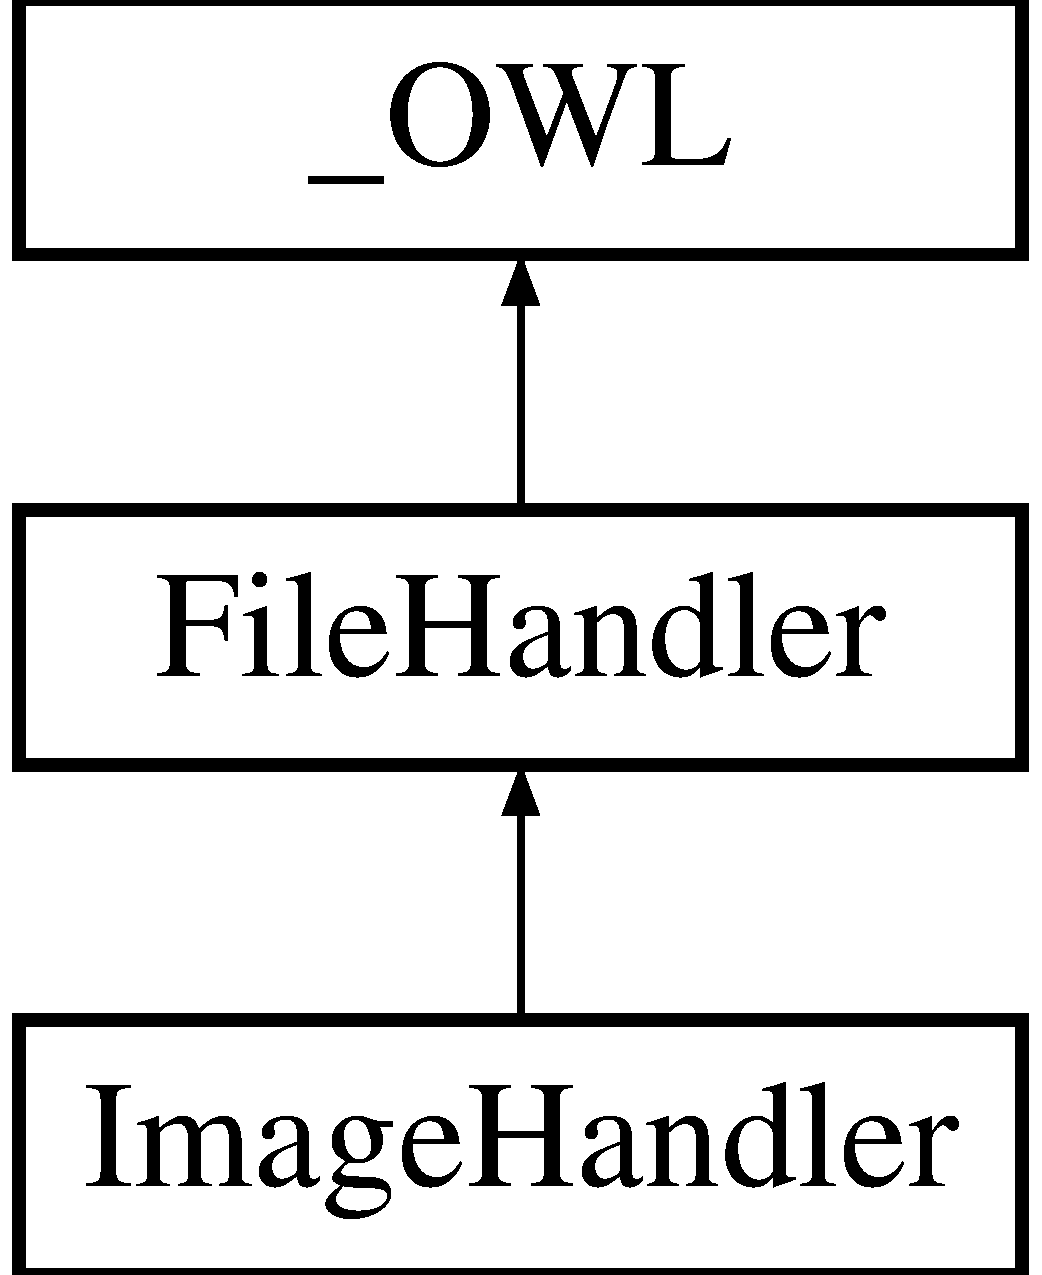
\includegraphics[height=3.000000cm]{classFileHandler}
\end{center}
\end{figure}
\subsection*{Public Member Functions}
\begin{DoxyCompactItemize}
\item 
{\bf \_\-\_\-construct} (\$name, \$req=false)
\item 
{\bf \_\-\_\-destruct} ()
\item 
{\bf encode} ()
\item 
{\bf download} ()
\item 
{\bf getLastWarning} ()
\item 
{\bf getStatus} ()
\item 
{\bf getSeverity} (\$status=null)
\item 
{\bf succeeded} (\$\_\-ok={\bf OWL\_\-SUCCESS}, \&\$\_\-object=null)
\item 
{\bf signal} (\$level={\bf OWL\_\-INFO}, \&\$text=false)
\item 
{\bf traceback} (\&\$text=false, \$depth=0)
\end{DoxyCompactItemize}
\subsection*{Public Attributes}
\begin{DoxyCompactItemize}
\item 
{\bf \$original\_\-name}
\end{DoxyCompactItemize}
\subsection*{Protected Member Functions}
\begin{DoxyCompactItemize}
\item 
{\bf open} (\$mode= 'r')
\item 
{\bf close} ()
\item 
{\bf readData} ()
\item 
{\bf readLine} (\$trim={\bf FILE\_\-NOTRIM})
\item 
{\bf init} ()
\item 
{\bf setCallback} (\$\_\-dispatcher)
\item 
{\bf setCallbackArgument} (array \$\_\-arg)
\item 
{\bf getCallback} ()
\item 
{\bf reset} ()
\item 
{\bf saveStatus} ()
\item 
{\bf restoreStatus} ()
\item 
{\bf check} (\&\$object, \$level={\bf OWL\_\-WARNING})
\item 
{\bf setStatus} (\$status, \$params=array())
\item 
{\bf setHighSeverity} (\&\$object=null)
\end{DoxyCompactItemize}
\subsection*{Protected Attributes}
\begin{DoxyCompactItemize}
\item 
{\bf \$name}
\item 
{\bf \$severity}
\end{DoxyCompactItemize}
\subsection*{Private Attributes}
\begin{DoxyCompactItemize}
\item 
{\bf \$fpointer}
\item 
{\bf \$opened}
\end{DoxyCompactItemize}


\subsection{Detailed Description}
File handler. 

Handle all files \begin{DoxyAuthor}{Author}
Oscar van Eijk, Oveas Functionality Provider 
\end{DoxyAuthor}
\begin{DoxyVersion}{Version}
May 15, 2007 -\/-\/ O van Eijk -\/-\/ initial version for Terra-\/Terra (based on an old OFM module) 

Jul 30, 2008 -\/-\/ O van Eijk -\/-\/ Modified version for OWL-\/PHP 
\end{DoxyVersion}


\subsection{Constructor \& Destructor Documentation}
\index{FileHandler@{FileHandler}!\_\-\_\-construct@{\_\-\_\-construct}}
\index{\_\-\_\-construct@{\_\-\_\-construct}!FileHandler@{FileHandler}}
\subsubsection[{\_\-\_\-construct}]{\setlength{\rightskip}{0pt plus 5cm}FileHandler::\_\-\_\-construct (
\begin{DoxyParamCaption}
\item[{\$}]{name, }
\item[{\$}]{req = {\ttfamily false}}
\end{DoxyParamCaption}
)}\label{classFileHandler_a8d75c8ea0c532acdeae0a0a4efa3704a}
Class constructor; setup the file characteristics 
\begin{DoxyParams}[1]{Parameters}
\mbox{\tt in}  & {\em \$name} & Filename \\
\hline
\mbox{\tt in}  & {\em \$req} & True is the file must exist at object create time \\
\hline
\end{DoxyParams}
\begin{DoxyAuthor}{Author}
Oscar van Eijk, Oveas Functionality Provider 
\end{DoxyAuthor}


Reimplemented in {\bf ImageHandler} \doxyref{}{p.}{classImageHandler_aa61dc81d4cf98eed31b32e2197018309}.



References \$name, \_\-OWL::init(), and \_\-OWL::setStatus().

\index{FileHandler@{FileHandler}!\_\-\_\-destruct@{\_\-\_\-destruct}}
\index{\_\-\_\-destruct@{\_\-\_\-destruct}!FileHandler@{FileHandler}}
\subsubsection[{\_\-\_\-destruct}]{\setlength{\rightskip}{0pt plus 5cm}FileHandler::\_\-\_\-destruct (
\begin{DoxyParamCaption}
{}
\end{DoxyParamCaption}
)}\label{classFileHandler_a734859e8962992da99dd8f853da5ae43}
Default class destructor \begin{DoxyAuthor}{Author}
Oscar van Eijk, Oveas Functionality Provider 
\end{DoxyAuthor}


Reimplemented from {\bf \_\-OWL} \doxyref{}{p.}{class__OWL_a44fd2222476a3109286cc82d92b6bbcc}.



References close().



\subsection{Member Function Documentation}
\index{FileHandler@{FileHandler}!check@{check}}
\index{check@{check}!FileHandler@{FileHandler}}
\subsubsection[{check}]{\setlength{\rightskip}{0pt plus 5cm}\_\-OWL::check (
\begin{DoxyParamCaption}
\item[{\&\$}]{object, }
\item[{\$}]{level = {\ttfamily {\bf OWL\_\-WARNING}}}
\end{DoxyParamCaption}
)\hspace{0.3cm}{\ttfamily  [protected, inherited]}}\label{class__OWL_ae2e3c56e5f3c4ce4156c6b1bb1c50f63}
This is a helper function for lazy developers. Some checks have to be made quite often, this is a kinda macro to handle that. It compares the own severity level with that of a given object. If the highest level is above a given max, a traceback and reset are performed.


\begin{DoxyParams}[1]{Parameters}
\mbox{\tt in}  & {\em \$object} & Pointer to an object to check against \\
\hline
\mbox{\tt in}  & {\em \$level} & The maximum severity level \\
\hline
\end{DoxyParams}
\begin{DoxyReturn}{Returns}
True if the severity level was correct (below the max), otherwise false 
\end{DoxyReturn}
\begin{DoxyAuthor}{Author}
Oscar van Eijk, Oveas Functionality Provider 
\end{DoxyAuthor}


References \_\-OWL::reset(), \_\-OWL::setHighSeverity(), and \_\-OWL::traceback().



Referenced by SessionHandler::write().

\index{FileHandler@{FileHandler}!close@{close}}
\index{close@{close}!FileHandler@{FileHandler}}
\subsubsection[{close}]{\setlength{\rightskip}{0pt plus 5cm}FileHandler::close (
\begin{DoxyParamCaption}
{}
\end{DoxyParamCaption}
)\hspace{0.3cm}{\ttfamily  [protected]}}\label{classFileHandler_aa48e7c3b67346e29b194d2f0ac5dd1f8}
Close the file \begin{DoxyAuthor}{Author}
Oscar van Eijk, Oveas Functionality Provider 
\end{DoxyAuthor}


References \_\-OWL::setStatus().



Referenced by \_\-\_\-destruct(), and readData().

\index{FileHandler@{FileHandler}!download@{download}}
\index{download@{download}!FileHandler@{FileHandler}}
\subsubsection[{download}]{\setlength{\rightskip}{0pt plus 5cm}FileHandler::download (
\begin{DoxyParamCaption}
{}
\end{DoxyParamCaption}
)}\label{classFileHandler_ac17edc9b92643c32ae6040b1235c64dd}
\index{FileHandler@{FileHandler}!encode@{encode}}
\index{encode@{encode}!FileHandler@{FileHandler}}
\subsubsection[{encode}]{\setlength{\rightskip}{0pt plus 5cm}FileHandler::encode (
\begin{DoxyParamCaption}
{}
\end{DoxyParamCaption}
)}\label{classFileHandler_aa29360bf94fd54d906256561f33d93ad}


References readData().

\index{FileHandler@{FileHandler}!getCallback@{getCallback}}
\index{getCallback@{getCallback}!FileHandler@{FileHandler}}
\subsubsection[{getCallback}]{\setlength{\rightskip}{0pt plus 5cm}\_\-OWL::getCallback (
\begin{DoxyParamCaption}
{}
\end{DoxyParamCaption}
)\hspace{0.3cm}{\ttfamily  [protected, inherited]}}\label{class__OWL_acb46ff88f43ca66f1268d3f5199c3f8d}
Retrieve a previously set (callback) dispatcher. The (callback) dispatcher is cleared immediatly. \begin{DoxyReturn}{Returns}
The dispatcher, of null on failure. 
\end{DoxyReturn}
\begin{DoxyAuthor}{Author}
Oscar van Eijk, Oveas Functionality Provider 
\end{DoxyAuthor}


Reimplemented in {\bf Dispatcher} \doxyref{}{p.}{classDispatcher_a31c4bd4e4eaee7ef90b1ea364a901447}.



References OWL::factory().

\index{FileHandler@{FileHandler}!getLastWarning@{getLastWarning}}
\index{getLastWarning@{getLastWarning}!FileHandler@{FileHandler}}
\subsubsection[{getLastWarning}]{\setlength{\rightskip}{0pt plus 5cm}\_\-OWL::getLastWarning (
\begin{DoxyParamCaption}
{}
\end{DoxyParamCaption}
)\hspace{0.3cm}{\ttfamily  [inherited]}}\label{class__OWL_a1888f52fc2d0ec29e146925ccad70a6b}
Get the last warning or error message. \begin{DoxyReturn}{Returns}
null if there was no error (severity below OWL\_\-WARNING), otherwise the error text. 
\end{DoxyReturn}
\begin{DoxyAuthor}{Author}
Oscar van Eijk, Oveas Functionality Provider 
\end{DoxyAuthor}


References \_\-OWL::signal().

\index{FileHandler@{FileHandler}!getSeverity@{getSeverity}}
\index{getSeverity@{getSeverity}!FileHandler@{FileHandler}}
\subsubsection[{getSeverity}]{\setlength{\rightskip}{0pt plus 5cm}\_\-OWL::getSeverity (
\begin{DoxyParamCaption}
\item[{\$}]{status = {\ttfamily null}}
\end{DoxyParamCaption}
)\hspace{0.3cm}{\ttfamily  [inherited]}}\label{class__OWL_a2374613f9bb7eccf49a5dbc9a9ef4751}
Get the current object severity level. 
\begin{DoxyParams}[1]{Parameters}
\mbox{\tt in}  & {\em \$status} & An optional parameter to check an other status code i.s.o the object's current status. \\
\hline
\end{DoxyParams}
\begin{DoxyReturn}{Returns}
Status severity level 
\end{DoxyReturn}
\begin{DoxyAuthor}{Author}
Oscar van Eijk, Oveas Functionality Provider 
\end{DoxyAuthor}


References \_\-OWL::\$status.



Referenced by LogHandler::composeMessage(), LogHandler::log(), and DataHandler::setKey().

\index{FileHandler@{FileHandler}!getStatus@{getStatus}}
\index{getStatus@{getStatus}!FileHandler@{FileHandler}}
\subsubsection[{getStatus}]{\setlength{\rightskip}{0pt plus 5cm}\_\-OWL::getStatus (
\begin{DoxyParamCaption}
{}
\end{DoxyParamCaption}
)\hspace{0.3cm}{\ttfamily  [final, inherited]}}\label{class__OWL_ac1f1643ff5b5db7c326c30477603358d}
Get the current object status. \begin{DoxyReturn}{Returns}
Object's status code 
\end{DoxyReturn}
\begin{DoxyAuthor}{Author}
Oscar van Eijk, Oveas Functionality Provider 
\end{DoxyAuthor}


Referenced by SchemeHandler::compare().

\index{FileHandler@{FileHandler}!init@{init}}
\index{init@{init}!FileHandler@{FileHandler}}
\subsubsection[{init}]{\setlength{\rightskip}{0pt plus 5cm}\_\-OWL::init (
\begin{DoxyParamCaption}
{}
\end{DoxyParamCaption}
)\hspace{0.3cm}{\ttfamily  [protected, inherited]}}\label{class__OWL_ae0ef3ded56e8a6b34b6461e5a721cd3e}
This function should be called by all constuctors. It initializes the general characteristics. Status is 'warning' by default, it's up to the contructor to set a proper status; if it's still 'warning', this $\ast$might$\ast$ indicate something went wrong. \begin{DoxyAuthor}{Author}
Oscar van Eijk, Oveas Functionality Provider 
\end{DoxyAuthor}


References OWL::factory(), and \_\-OWL::setStatus().



Referenced by FormFieldPlugin::\_\-\_\-construct(), Document::\_\-\_\-construct(), ContainerPlugin::\_\-\_\-construct(), Container::\_\-\_\-construct(), SocketHandler::\_\-\_\-construct(), SessionHandler::\_\-\_\-construct(), SchemeHandler::\_\-\_\-construct(), LogHandler::\_\-\_\-construct(), ImageHandler::\_\-\_\-construct(), FormHandler::\_\-\_\-construct(), \_\-\_\-construct(), DbHandler::\_\-\_\-construct(), HDataHandler::\_\-\_\-construct(), DataHandler::\_\-\_\-construct(), OWL::\_\-\_\-construct(), Mail::\_\-\_\-construct(), Group::\_\-\_\-construct(), Form::\_\-\_\-construct(), Dispatcher::\_\-\_\-construct(), and User::construct().

\index{FileHandler@{FileHandler}!open@{open}}
\index{open@{open}!FileHandler@{FileHandler}}
\subsubsection[{open}]{\setlength{\rightskip}{0pt plus 5cm}FileHandler::open (
\begin{DoxyParamCaption}
\item[{\$}]{mode = {\ttfamily 'r'}}
\end{DoxyParamCaption}
)\hspace{0.3cm}{\ttfamily  [protected]}}\label{classFileHandler_a2a650b033c4eb1f98ba47fb05ce7b454}
Open the file 
\begin{DoxyParams}[1]{Parameters}
\mbox{\tt in}  & {\em \$mode} & Mode in which the file should be opened:
\begin{DoxyItemize}
\item 'r' Open for reading only; place the file pointer at the beginning of the file.
\item 'r+' Open for reading and writing; place the file pointer at the beginning of the file.
\item 'w' Open for writing only; place the file pointer at the beginning of the file and truncate the file to zero length. If the file does not exist, attempt to create it.
\item 'w+' Open for reading and writing; place the file pointer at the beginning of the file and truncate the file to zero length. If the file does not exist, attempt to create it.
\item 'a' Open for writing only; place the file pointer at the end of the file. If the file does not exist, attempt to create it.
\item 'a+' Open for reading and writing; place the file pointer at the end of the file. If the file does not exist, attempt to create it. 
\end{DoxyItemize}\\
\hline
\end{DoxyParams}
\begin{DoxyAuthor}{Author}
Oscar van Eijk, Oveas Functionality Provider 
\end{DoxyAuthor}


References \_\-OWL::setStatus().



Referenced by readData().

\index{FileHandler@{FileHandler}!readData@{readData}}
\index{readData@{readData}!FileHandler@{FileHandler}}
\subsubsection[{readData}]{\setlength{\rightskip}{0pt plus 5cm}FileHandler::readData (
\begin{DoxyParamCaption}
{}
\end{DoxyParamCaption}
)\hspace{0.3cm}{\ttfamily  [protected]}}\label{classFileHandler_a6f9263704f08f071a5e563aeb3216d95}
Read the file contents and return as one dataset \begin{DoxyAuthor}{Author}
Oscar van Eijk, Oveas Functionality Provider 
\end{DoxyAuthor}


References close(), and open().



Referenced by encode().

\index{FileHandler@{FileHandler}!readLine@{readLine}}
\index{readLine@{readLine}!FileHandler@{FileHandler}}
\subsubsection[{readLine}]{\setlength{\rightskip}{0pt plus 5cm}FileHandler::readLine (
\begin{DoxyParamCaption}
\item[{\$}]{trim = {\ttfamily {\bf FILE\_\-NOTRIM}}}
\end{DoxyParamCaption}
)\hspace{0.3cm}{\ttfamily  [protected]}}\label{classFileHandler_a2140ee43c68f088396b4573a56e3007c}
Read a single line from the file. File must be opened before 
\begin{DoxyParams}[1]{Parameters}
\mbox{\tt in}  & {\em \$trim} & specify how the returned line should be trimmed:
\begin{DoxyItemize}
\item FILE\_\-NOTRIM
\item FILE\_\-TRIM\_\-L
\item FILE\_\-TRIM\_\-R
\item FILE\_\-TRIM\_\-C 
\end{DoxyItemize}\\
\hline
\end{DoxyParams}
\begin{DoxyAuthor}{Author}
Oscar van Eijk, Oveas Functionality Provider 
\end{DoxyAuthor}


References \_\-OWL::setStatus().

\index{FileHandler@{FileHandler}!reset@{reset}}
\index{reset@{reset}!FileHandler@{FileHandler}}
\subsubsection[{reset}]{\setlength{\rightskip}{0pt plus 5cm}\_\-OWL::reset (
\begin{DoxyParamCaption}
{}
\end{DoxyParamCaption}
)\hspace{0.3cm}{\ttfamily  [protected, inherited]}}\label{class__OWL_a2f2a042bcf31965194c03033df0edc9b}
General reset function for all objects. Should be called after each non-\/fatal error \begin{DoxyAuthor}{Author}
Oscar van Eijk, Oveas Functionality Provider 
\end{DoxyAuthor}


Reimplemented in {\bf DbHandler} \doxyref{}{p.}{classDbHandler_a9982df4830f05803935bb31bac7fae3d}, and {\bf SchemeHandler} \doxyref{}{p.}{classSchemeHandler_aa25feb4a70d67b3d571904be4b2f50bc}.



References \_\-OWL::resetCalltree().



Referenced by \_\-OWL::check(), SessionHandler::read(), DataHandler::reset(), and \_\-OWL::setStatus().

\index{FileHandler@{FileHandler}!restoreStatus@{restoreStatus}}
\index{restoreStatus@{restoreStatus}!FileHandler@{FileHandler}}
\subsubsection[{restoreStatus}]{\setlength{\rightskip}{0pt plus 5cm}\_\-OWL::restoreStatus (
\begin{DoxyParamCaption}
{}
\end{DoxyParamCaption}
)\hspace{0.3cm}{\ttfamily  [protected, inherited]}}\label{class__OWL_a93de01a9bbbc3f228e1a62a0740e90f0}
Restore the previously saved status object and destroy the copy \begin{DoxyAuthor}{Author}
Oscar van Eijk, Oveas Functionality Provider 
\end{DoxyAuthor}


References \_\-OWL::setStatus().



Referenced by User::logout().

\index{FileHandler@{FileHandler}!saveStatus@{saveStatus}}
\index{saveStatus@{saveStatus}!FileHandler@{FileHandler}}
\subsubsection[{saveStatus}]{\setlength{\rightskip}{0pt plus 5cm}\_\-OWL::saveStatus (
\begin{DoxyParamCaption}
{}
\end{DoxyParamCaption}
)\hspace{0.3cm}{\ttfamily  [protected, inherited]}}\label{class__OWL_add923dc756471318edca8883db3f4420}
Create a copy of the status object \begin{DoxyAuthor}{Author}
Oscar van Eijk, Oveas Functionality Provider 
\end{DoxyAuthor}


Referenced by User::logout().

\index{FileHandler@{FileHandler}!setCallback@{setCallback}}
\index{setCallback@{setCallback}!FileHandler@{FileHandler}}
\subsubsection[{setCallback}]{\setlength{\rightskip}{0pt plus 5cm}\_\-OWL::setCallback (
\begin{DoxyParamCaption}
\item[{\$}]{\_\-dispatcher}
\end{DoxyParamCaption}
)\hspace{0.3cm}{\ttfamily  [protected, inherited]}}\label{class__OWL_a5f84d43cd4dc7810649f1e2ebecad360}
Set a dispatcher for later callback 
\begin{DoxyParams}[1]{Parameters}
\mbox{\tt in}  & {\em \$\_\-dispatcher} & Dispatched, \\
\hline
\end{DoxyParams}
\begin{DoxySeeAlso}{See also}
\doxyref{Dispatcher::composeDispatcher()}{p.}{classDispatcher_a8a974bbbb30be7cda74f9929972fd2f6} 
\end{DoxySeeAlso}
\begin{DoxyReturn}{Returns}
True on success, false on failure 
\end{DoxyReturn}
\begin{DoxyAuthor}{Author}
Oscar van Eijk, Oveas Functionality Provider 
\end{DoxyAuthor}


References OWL::factory().

\index{FileHandler@{FileHandler}!setCallbackArgument@{setCallbackArgument}}
\index{setCallbackArgument@{setCallbackArgument}!FileHandler@{FileHandler}}
\subsubsection[{setCallbackArgument}]{\setlength{\rightskip}{0pt plus 5cm}\_\-OWL::setCallbackArgument (
\begin{DoxyParamCaption}
\item[{array \$}]{\_\-arg}
\end{DoxyParamCaption}
)\hspace{0.3cm}{\ttfamily  [protected, inherited]}}\label{class__OWL_a4e9ebfbd3c0d76539bed4e44de9962c3}
Add an argument to a previously registered callback dispatcher 
\begin{DoxyParams}[1]{Parameters}
\mbox{\tt in}  & {\em \$\_\-arg} & Argument, must be an array type. When non-\/ arrays should be passed as arguments, the must be set when the callback is registered already \\
\hline
\end{DoxyParams}
\begin{DoxyReturn}{Returns}
True on success, false on failure 
\end{DoxyReturn}
\begin{DoxyAuthor}{Author}
Oscar van Eijk, Oveas Functionality Provider 
\end{DoxyAuthor}


References OWL::factory().



Referenced by User::register().

\index{FileHandler@{FileHandler}!setHighSeverity@{setHighSeverity}}
\index{setHighSeverity@{setHighSeverity}!FileHandler@{FileHandler}}
\subsubsection[{setHighSeverity}]{\setlength{\rightskip}{0pt plus 5cm}\_\-OWL::setHighSeverity (
\begin{DoxyParamCaption}
\item[{\&\$}]{object = {\ttfamily null}}
\end{DoxyParamCaption}
)\hspace{0.3cm}{\ttfamily  [protected, inherited]}}\label{class__OWL_a97173dbe452428d3851406413264734d}
Compare the severity level of the current object with a given one and set my statuspointer to the object with the highest level. \begin{DoxyAuthor}{Author}
Oscar van Eijk, Oveas Functionality Provider 
\end{DoxyAuthor}


Referenced by \_\-OWL::check(), DataHandler::db(), DataHandler::prepare(), and SessionHandler::read().

\index{FileHandler@{FileHandler}!setStatus@{setStatus}}
\index{setStatus@{setStatus}!FileHandler@{FileHandler}}
\subsubsection[{setStatus}]{\setlength{\rightskip}{0pt plus 5cm}\_\-OWL::setStatus (
\begin{DoxyParamCaption}
\item[{\$}]{status, }
\item[{\$}]{params = {\ttfamily array~()}}
\end{DoxyParamCaption}
)\hspace{0.3cm}{\ttfamily  [final, protected, inherited]}}\label{class__OWL_a80e2fe01c3663dbb0ab685eebe33fd1e}
Set the current object status to the specified value. 
\begin{DoxyParams}[1]{Parameters}
\mbox{\tt in}  & {\em \$status} & \doxyref{OWL}{p.}{classOWL} status code \\
\hline
\mbox{\tt in}  & {\em \$params} & \\
\hline
\end{DoxyParams}
\begin{DoxyAuthor}{Author}
Oscar van Eijk, Oveas Functionality Provider 
\end{DoxyAuthor}


References \$GLOBALS, \_\-OWL::\$status, ConfigHandler::get(), Register::getCode(), \_\-OWL::reset(), and \_\-OWL::signal().



Referenced by DbHandler::\_\-\_\-clone(), Container::\_\-\_\-construct(), SocketHandler::\_\-\_\-construct(), SchemeHandler::\_\-\_\-construct(), ImageHandler::\_\-\_\-construct(), FormHandler::\_\-\_\-construct(), \_\-\_\-construct(), DbHandler::\_\-\_\-construct(), DataHandler::\_\-\_\-construct(), Session::\_\-\_\-construct(), Mail::\_\-\_\-construct(), BaseElement::\_\-getContent(), HDataHandler::\_\-getNewLeft(), Mail::addBcc(), Mail::addCc(), Container::addContainer(), Form::addField(), FormFieldRadioPlugin::addOption(), HDataHandler::addParent(), Mail::addTo(), BaseElement::addToContent(), DbHandler::alt(), SchemeHandler::alterScheme(), close(), DbHandler::commitTransaction(), Dispatcher::composeDispatcher(), User::confirm(), SocketHandler::connect(), DbHandler::connect(), DbHandler::create(), SchemeHandler::createScheme(), DbHandler::dbread(), SchemeHandler::defineIndex(), SchemeHandler::defineScheme(), SocketHandler::disconnect(), Dispatcher::dispatch(), HDataHandler::enableCrossLink(), FormHandler::get(), DataHandler::get(), HDataHandler::getDirectChildren(), HDataHandler::getFullOffspring(), Group::getGroupByName(), SchemeHandler::getTableColumns(), SchemeHandler::getTableIndexes(), \_\-OWL::init(), Document::loadScript(), Document::loadStyle(), DbHandler::lockTable(), User::login(), HDataHandler::moveNode(), open(), DbHandler::open(), LogHandler::openLogfile(), DataHandler::prepare(), DbHandler::prepareDelete(), DbHandler::prepareField(), DbHandler::prepareInsert(), DbHandler::prepareRead(), DbHandler::prepareUpdate(), SocketHandler::read(), DbHandler::read(), readLine(), HDataHandler::readQuery(), User::readUserdata(), User::register(), Dispatcher::registerArgument(), Dispatcher::registerCallback(), DbHandler::resetTable(), \_\-OWL::restoreStatus(), DbHandler::rollbackTransaction(), SchemeHandler::scheme(), Mail::send(), FormHandler::set(), BaseElement::setAttributes(), BaseElement::setContent(), Form::setEncoding(), Document::setFavicon(), Form::setFieldAttributes(), Mail::setFrom(), DataHandler::setJoin(), DataHandler::setKey(), FormFieldTextPlugin::setMaxsize(), Document::setMeta(), Form::setMethod(), FormFieldRadioPlugin::setSelected(), Mail::setSender(), FormFieldTextPlugin::setSize(), FormFieldSelectPlugin::setSize(), FormFieldSelectPlugin::setValue(), Form::showField(), DbHandler::startTransaction(), SchemeHandler::tableDescription(), DbHandler::unlockTable(), SchemeHandler::validateScheme(), SocketHandler::write(), DbHandler::write(), and HDataHandler::writeQuery().

\index{FileHandler@{FileHandler}!signal@{signal}}
\index{signal@{signal}!FileHandler@{FileHandler}}
\subsubsection[{signal}]{\setlength{\rightskip}{0pt plus 5cm}\_\-OWL::signal (
\begin{DoxyParamCaption}
\item[{\$}]{level = {\ttfamily {\bf OWL\_\-INFO}}, }
\item[{\&\$}]{text = {\ttfamily false}}
\end{DoxyParamCaption}
)\hspace{0.3cm}{\ttfamily  [inherited]}}\label{class__OWL_a51ba4a16409acf2a2f61f286939091a5}
Display the message for the current object status 
\begin{DoxyParams}[1]{Parameters}
\mbox{\tt in}  & {\em \$level} & An optional severity level; message will only be displayed when it is at least of this level. \\
\hline
\mbox{\tt out}  & {\em \$text} & If this parameter is given, the message text is returned in this string instead of echood. \\
\hline
\end{DoxyParams}
\begin{DoxyReturn}{Returns}
The severity level for this object 
\end{DoxyReturn}
\begin{DoxyAuthor}{Author}
Oscar van Eijk, Oveas Functionality Provider 
\end{DoxyAuthor}


References ConfigHandler::get().



Referenced by \_\-OWL::getLastWarning(), \_\-OWL::setStatus(), and \_\-OWL::traceback().

\index{FileHandler@{FileHandler}!succeeded@{succeeded}}
\index{succeeded@{succeeded}!FileHandler@{FileHandler}}
\subsubsection[{succeeded}]{\setlength{\rightskip}{0pt plus 5cm}\_\-OWL::succeeded (
\begin{DoxyParamCaption}
\item[{\$}]{\_\-ok = {\ttfamily {\bf OWL\_\-SUCCESS}}, }
\item[{\&\$}]{\_\-object = {\ttfamily null}}
\end{DoxyParamCaption}
)\hspace{0.3cm}{\ttfamily  [inherited]}}\label{class__OWL_a53ab4d3bbb2c6a56966c339ca4b4c805}
Check if the object currenlty has a success state 
\begin{DoxyParams}[1]{Parameters}
\mbox{\tt in}  & {\em \$\_\-ok} & The highest severity that's considered successfull, default OWL\_\-SUCCESS \\
\hline
\mbox{\tt in}  & {\em \$\_\-object} & REference to the object to check, defaults to the current object \\
\hline
\end{DoxyParams}
\begin{DoxyReturn}{Returns}
Boolean true when successfull 
\end{DoxyReturn}
\begin{DoxyAuthor}{Author}
Oscar van Eijk, Oveas Functionality Provider 
\end{DoxyAuthor}


Referenced by User::construct(), Dispatcher::registerArgument(), and Dispatcher::registerCallback().

\index{FileHandler@{FileHandler}!traceback@{traceback}}
\index{traceback@{traceback}!FileHandler@{FileHandler}}
\subsubsection[{traceback}]{\setlength{\rightskip}{0pt plus 5cm}\_\-OWL::traceback (
\begin{DoxyParamCaption}
\item[{\&\$}]{text = {\ttfamily false}, }
\item[{\$}]{depth = {\ttfamily 0}}
\end{DoxyParamCaption}
)\hspace{0.3cm}{\ttfamily  [inherited]}}\label{class__OWL_aa29547995d6741b7d2b90c1d4ea99a13}
If somehwere in the nested calls an error occured, we can traceback the original failing object with this function and signal the message. 
\begin{DoxyParams}[1]{Parameters}
\mbox{\tt out}  & {\em \$text} & Optional variable in which the message text can be stored. If not given, the text will be written to standard output \\
\hline
\mbox{\tt in}  & {\em \$depth} & This paramater should be initially empty. It calculates the depth in recursive calls. \\
\hline
\end{DoxyParams}
\begin{DoxyReturn}{Returns}
Severity code of the failing object 
\end{DoxyReturn}
\begin{DoxyAuthor}{Author}
Oscar van Eijk, Oveas Functionality Provider 
\end{DoxyAuthor}


References \_\-OWL::signal().



Referenced by \_\-OWL::check(), User::login(), and SessionHandler::read().



\subsection{Member Data Documentation}
\index{FileHandler@{FileHandler}!\$fpointer@{\$fpointer}}
\index{\$fpointer@{\$fpointer}!FileHandler@{FileHandler}}
\subsubsection[{\$fpointer}]{\setlength{\rightskip}{0pt plus 5cm}FileHandler::\$fpointer\hspace{0.3cm}{\ttfamily  [private]}}\label{classFileHandler_aa0aa66fd3ad551b3f508b901a95c0c2d}
Pointer to te file when opened 

Reimplemented in {\bf ImageHandler} \doxyref{}{p.}{classImageHandler_ac56acda82f7ece75d33f6c57845a727e}.

\index{FileHandler@{FileHandler}!\$name@{\$name}}
\index{\$name@{\$name}!FileHandler@{FileHandler}}
\subsubsection[{\$name}]{\setlength{\rightskip}{0pt plus 5cm}FileHandler::\$name\hspace{0.3cm}{\ttfamily  [protected]}}\label{classFileHandler_a94903bd51b241928ed415ad271c38805}
Full filename as stored on the file system 

Reimplemented in {\bf ImageHandler} \doxyref{}{p.}{classImageHandler_a517b3d7ff8643cca1dc2080523bfe2d6}.



Referenced by \_\-\_\-construct().

\index{FileHandler@{FileHandler}!\$opened@{\$opened}}
\index{\$opened@{\$opened}!FileHandler@{FileHandler}}
\subsubsection[{\$opened}]{\setlength{\rightskip}{0pt plus 5cm}FileHandler::\$opened\hspace{0.3cm}{\ttfamily  [private]}}\label{classFileHandler_a061409b2bbd2e13bc47415527c0de720}
Boolean that's true when the file is opened 

Reimplemented in {\bf ImageHandler} \doxyref{}{p.}{classImageHandler_a6a87b3626bd0a457c6937b3e9b1cc69b}.

\index{FileHandler@{FileHandler}!\$original\_\-name@{\$original\_\-name}}
\index{\$original\_\-name@{\$original\_\-name}!FileHandler@{FileHandler}}
\subsubsection[{\$original\_\-name}]{\setlength{\rightskip}{0pt plus 5cm}FileHandler::\$original\_\-name}\label{classFileHandler_a477708585850c3c8725ccf56bfe0b4a8}


Reimplemented in {\bf ImageHandler} \doxyref{}{p.}{classImageHandler_a1712c9444d65879aab111260767afaab}.

\index{FileHandler@{FileHandler}!\$severity@{\$severity}}
\index{\$severity@{\$severity}!FileHandler@{FileHandler}}
\subsubsection[{\$severity}]{\setlength{\rightskip}{0pt plus 5cm}\_\-OWL::\$severity\hspace{0.3cm}{\ttfamily  [protected, inherited]}}\label{class__OWL_ad26b40a9dbbacb33e299b17826f8327c}
Severity level of the current object status 

The documentation for this class was generated from the following file:\begin{DoxyCompactItemize}
\item 
/home/oscar/projects/owl-\/php/src/kernel/so/{\bf class.filehandler.php}\end{DoxyCompactItemize}

\section{Form Class Reference}
\label{classForm}\index{Form@{Form}}


\hyperlink{classForm}{Form} Element class.  




Inheritance diagram for Form:
\nopagebreak
\begin{figure}[H]
\begin{center}
\leavevmode
\includegraphics[height=600pt]{classForm__inherit__graph}
\end{center}
\end{figure}


Collaboration diagram for Form:
\nopagebreak
\begin{figure}[H]
\begin{center}
\leavevmode
\includegraphics[height=600pt]{classForm__coll__graph}
\end{center}
\end{figure}
\subsection*{Public Member Functions}
\begin{DoxyCompactItemize}
\item 
\hyperlink{classForm_ae90293f5520279d6c18f416d3f883ac8}{\_\-\_\-construct} (\$\_\-dispatcher, \$\_\-attribs=array())
\item 
\hyperlink{classForm_a2dc6461afb09effeefe444847ad9b562}{setMethod} (\$method)
\item 
\hyperlink{classForm_a2b1f9bb23c4da0558002b62f60b55078}{setEncoding} (\$enctype)
\item 
\hyperlink{classForm_a880197a858a70581146d6f0d275eff02}{addField} (\$type, \$name, \$value= '', \$attributes=array())
\item 
\hyperlink{classForm_a83cd5bed7649ecfe202dd97a8129f6f8}{setFieldAttributes} (\$index, \$attributes)
\item 
\hyperlink{classForm_a011360ce04a237f5609446f3134ec32c}{setFieldEvents} (\$index, \$events)
\item 
\hyperlink{classForm_a29e01263557e33fab02ee5c3aaa0b3f5}{showField} (\$name)
\item 
\hyperlink{classForm_aeac5855c8b2406c34090a621d59df664}{showElement} ()
\item 
\hyperlink{classBaseElement_a0c1ce3d1684ecb78960cf7a97278494e}{setId} (\$\_\-value)
\item 
\hyperlink{classBaseElement_a4a7aa583ee21af392908d7fd42fde790}{getId} ()
\item 
\hyperlink{classBaseElement_a39bafb3609d10048920c20242c2a04c5}{setName} (\$\_\-value)
\item 
\hyperlink{classBaseElement_a6b2b9ff69f6e92db82f91d9c55cda697}{setStyle} (\$\_\-value)
\item 
\hyperlink{classBaseElement_af6597b30fa9798878f6290271043dfa2}{setClass} (\$\_\-value)
\item 
\hyperlink{classBaseElement_a164a9c6e4ee68afa0ad343942ba54d28}{setContent} (\&\$\_\-content)
\item 
\hyperlink{classBaseElement_abd48eef64ca4f419f26d66a0c0419908}{addToContent} (\&\$\_\-content)
\item 
\hyperlink{classBaseElement_af8c86b93bcdcfbc415bf96c622dc5516}{getContent} ()
\item 
\hyperlink{classBaseElement_ad5789f45f16aaa144716ee8558069c31}{setEvent} (\$\_\-event, \$\_\-action, \$\_\-add=false)
\item 
\hyperlink{classBaseElement_aa623b042d23a5b77add8b3c452ec5855}{setAttributes} (\$\_\-attribs)
\item 
\hyperlink{class__OWL_a99ec771fa2c5c279f80152cc09e489a8}{get\_\-status} ()
\item 
\hyperlink{class__OWL_adf9509ef96858be7bdd9414c5ef129aa}{get\_\-severity} (\$status=null)
\item 
\hyperlink{class__OWL_a51ba4a16409acf2a2f61f286939091a5}{signal} (\$level=\hyperlink{owl_8severitycodes_8php_a139328861128689f2f4def6a399d9057}{OWL\_\-INFO}, \&\$text=false)
\item 
\hyperlink{class__OWL_aa29547995d6741b7d2b90c1d4ea99a13}{traceback} (\&\$text=false, \$depth=0)
\end{DoxyCompactItemize}
\subsection*{Protected Member Functions}
\begin{DoxyCompactItemize}
\item 
\hyperlink{classBaseElement_ae8237038633fc53db818f36da1940297}{getAttributes} (\$\_\-ignore=array())
\item 
\hyperlink{class__OWL_ae0ef3ded56e8a6b34b6461e5a721cd3e}{init} ()
\item 
\hyperlink{class__OWL_a2f2a042bcf31965194c03033df0edc9b}{reset} ()
\item 
\hyperlink{class__OWL_a9e49b9c76fbc021b244c6915ea536d71}{save\_\-status} ()
\item 
\hyperlink{class__OWL_a465eeaf40edd9f9c848841700c32ce55}{restore\_\-status} ()
\item 
\hyperlink{class__OWL_ad6f4f6946f40199dd0333cf219fa500e}{check} (\&\$object, \$level)
\item 
\hyperlink{class__OWL_aea912d0ede9b3c2a69b79072d94d4787}{set\_\-status} (\$status, \$params=array())
\item 
\hyperlink{class__OWL_a576829692a3b66e3d518853bf43abae3}{set\_\-high\_\-severity} (\&\$object=null)
\end{DoxyCompactItemize}
\subsection*{Protected Attributes}
\begin{DoxyCompactItemize}
\item 
\hyperlink{classBaseElement_a99976a8e967db92e7800309f359b0803}{\$class} = ''
\item 
\hyperlink{classBaseElement_a429a3d642dd95f30e1059ef29564b87d}{\$style} = ''
\item 
\hyperlink{classBaseElement_a02cebe45d277b4ff8f29db08bad371ba}{\$events} = array()
\item 
\hyperlink{classBaseElement_a30b8cff187a9de659a70daf287d66f45}{\$name} = ''
\item 
\hyperlink{classBaseElement_a11b6989c43b53869a09f5ce65aa55b45}{\$id} = ''
\item 
\hyperlink{class__OWL_ad26b40a9dbbacb33e299b17826f8327c}{\$severity}
\end{DoxyCompactItemize}
\subsection*{Private Member Functions}
\begin{DoxyCompactItemize}
\item 
\hyperlink{classForm_a94902cc2869e1608247d9204036af7d1}{openForm} ()
\item 
\hyperlink{classForm_a9bb2df9ed7b866b0dc4b29b3874c2a1a}{closeForm} ()
\end{DoxyCompactItemize}
\subsection*{Private Attributes}
\begin{DoxyCompactItemize}
\item 
\hyperlink{classForm_abcb1c4022c2b93073a00ae65f3269d5b}{\$fields}
\item 
\hyperlink{classForm_ab02292e715af1dc9b0499dd20900aa92}{\$dispatcher}
\item 
\hyperlink{classForm_a3ca31ec7032a41b95c94de22a850672c}{\$method}
\item 
\hyperlink{classForm_a9c23b3ec186995d3df3ad6d4d5efc134}{\$enctype}
\end{DoxyCompactItemize}


\subsection{Detailed Description}
\hyperlink{classForm}{Form} Element class. Define an HTML \hyperlink{classForm}{Form}. \begin{DoxyAuthor}{Author}
Oscar van Eijk, Oveas Functionality Provider 
\end{DoxyAuthor}
\begin{DoxyVersion}{Version}
Aug 29, 2008 -\/-\/ O van Eijk -\/-\/ initial version 
\end{DoxyVersion}


\subsection{Constructor \& Destructor Documentation}
\index{Form@{Form}!\_\-\_\-construct@{\_\-\_\-construct}}
\index{\_\-\_\-construct@{\_\-\_\-construct}!Form@{Form}}
\subsubsection[{\_\-\_\-construct}]{\setlength{\rightskip}{0pt plus 5cm}Form::\_\-\_\-construct (
\begin{DoxyParamCaption}
\item[{\$}]{ \_\-dispatcher, }
\item[{\$}]{ \_\-attribs = {\ttfamily array()}}
\end{DoxyParamCaption}
)}\label{classForm_ae90293f5520279d6c18f416d3f883ac8}
Class constructor 
\begin{DoxyParams}{Parameters}
\item[\mbox{\tt[in]} {\em \$\_\-dispatcher}]\hyperlink{classOWL}{OWL} dispatcher as string or array, \end{DoxyParams}
\begin{DoxySeeAlso}{See also}
\hyperlink{classDispatcher_a8a974bbbb30be7cda74f9929972fd2f6}{Dispatcher::composeDispatcher()} 
\end{DoxySeeAlso}

\begin{DoxyParams}{Parameters}
\item[\mbox{\tt[in]} {\em \$\_\-attribs}]Indexed array with the HTML attributes \end{DoxyParams}


References OWL::factory(), \_\-OWL::init(), and BaseElement::setAttributes().



\subsection{Member Function Documentation}
\index{Form@{Form}!addField@{addField}}
\index{addField@{addField}!Form@{Form}}
\subsubsection[{addField}]{\setlength{\rightskip}{0pt plus 5cm}Form::addField (
\begin{DoxyParamCaption}
\item[{\$}]{ type, }
\item[{\$}]{ name, }
\item[{\$}]{ value = {\ttfamily ''}, }
\item[{\$}]{ attributes = {\ttfamily array()}}
\end{DoxyParamCaption}
)}\label{classForm_a880197a858a70581146d6f0d275eff02}
Add a formfield to the formelement 
\begin{DoxyParams}{Parameters}
\item[\mbox{\tt[in]} {\em \$type}]Field type \item[\mbox{\tt[in]} {\em \$name}]Field name \item[\mbox{\tt[in]} {\em \$value}]Optional field value. For a selectlist type this must be an array, see FormFieldSelect::setValue() \item[\mbox{\tt[in]} {\em \$attributes}]Indexed array with additional values in the format, where the key must be a supported attributed for the given type. \end{DoxyParams}
\begin{DoxyReturn}{Returns}
Reference to the field object, or the severity in case of errors 
\end{DoxyReturn}


References BaseElement::\$name, OWLloader::getClass(), \_\-OWL::set\_\-status(), and setFieldAttributes().



Referenced by closeForm().

\index{Form@{Form}!addToContent@{addToContent}}
\index{addToContent@{addToContent}!Form@{Form}}
\subsubsection[{addToContent}]{\setlength{\rightskip}{0pt plus 5cm}BaseElement::addToContent (
\begin{DoxyParamCaption}
\item[{\&\$}]{ \_\-content}
\end{DoxyParamCaption}
)\hspace{0.3cm}{\ttfamily  \mbox{[}inherited\mbox{]}}}\label{classBaseElement_abd48eef64ca4f419f26d66a0c0419908}
Add a content to the container. If the container is not an array yet, it will be converted to obe. 
\begin{DoxyParams}{Parameters}
\item[\mbox{\tt[in]} {\em \$\_\-content}]Reference to the content, which can be HTML code or an object, of which the \hyperlink{classBaseElement_a63634d81fad745e3b72cda0100afebea}{showElement()} method will be called to retrieve the HTML. \end{DoxyParams}


References \_\-OWL::set\_\-status().

\index{Form@{Form}!check@{check}}
\index{check@{check}!Form@{Form}}
\subsubsection[{check}]{\setlength{\rightskip}{0pt plus 5cm}\_\-OWL::check (
\begin{DoxyParamCaption}
\item[{\&\$}]{ object, }
\item[{\$}]{ level}
\end{DoxyParamCaption}
)\hspace{0.3cm}{\ttfamily  \mbox{[}protected, inherited\mbox{]}}}\label{class__OWL_ad6f4f6946f40199dd0333cf219fa500e}
This is a helper function for lazy developers. Some checks have to be made quite often, this is a kinda macro to handle that. It compares the own severity level with that of a given object. If the highest level is above a given max, a traceback and reset are performed.


\begin{DoxyParams}{Parameters}
\item[\mbox{\tt[in]} {\em \$object}]Pointer to an object to check against \item[\mbox{\tt[in]} {\em \$level}]The maximum severity level \end{DoxyParams}
\begin{DoxyReturn}{Returns}
True if the severity level was correct ( below the max), otherwise false 
\end{DoxyReturn}


References \_\-OWL::reset(), \_\-OWL::set\_\-high\_\-severity(), and \_\-OWL::traceback().



Referenced by SessionHandler::write().

\index{Form@{Form}!closeForm@{closeForm}}
\index{closeForm@{closeForm}!Form@{Form}}
\subsubsection[{closeForm}]{\setlength{\rightskip}{0pt plus 5cm}Form::closeForm (
\begin{DoxyParamCaption}
{}
\end{DoxyParamCaption}
)\hspace{0.3cm}{\ttfamily  \mbox{[}private\mbox{]}}}\label{classForm_a9bb2df9ed7b866b0dc4b29b3874c2a1a}
Close the form and set a hidden field defining the dispatcher \begin{DoxyReturn}{Returns}
HTML code 
\end{DoxyReturn}


References addField(), and showField().



Referenced by showElement().

\index{Form@{Form}!get\_\-severity@{get\_\-severity}}
\index{get\_\-severity@{get\_\-severity}!Form@{Form}}
\subsubsection[{get\_\-severity}]{\setlength{\rightskip}{0pt plus 5cm}\_\-OWL::get\_\-severity (
\begin{DoxyParamCaption}
\item[{\$}]{ status = {\ttfamily null}}
\end{DoxyParamCaption}
)\hspace{0.3cm}{\ttfamily  \mbox{[}inherited\mbox{]}}}\label{class__OWL_adf9509ef96858be7bdd9414c5ef129aa}
Get the current object severity level.


\begin{DoxyParams}{Parameters}
\item[\mbox{\tt[in]} {\em \$status}]An optional parameter to check an other status code i.s.o the object's current status. \end{DoxyParams}
\begin{DoxyReturn}{Returns}
Status severity level 
\end{DoxyReturn}


References \_\-OWL::\$status.



Referenced by LogHandler::compose\_\-message(), LogHandler::log(), and DataHandler::set\_\-key().

\index{Form@{Form}!get\_\-status@{get\_\-status}}
\index{get\_\-status@{get\_\-status}!Form@{Form}}
\subsubsection[{get\_\-status}]{\setlength{\rightskip}{0pt plus 5cm}\_\-OWL::get\_\-status (
\begin{DoxyParamCaption}
{}
\end{DoxyParamCaption}
)\hspace{0.3cm}{\ttfamily  \mbox{[}final, inherited\mbox{]}}}\label{class__OWL_a99ec771fa2c5c279f80152cc09e489a8}
Get the current object status.

\begin{DoxyReturn}{Returns}
Object's status code 
\end{DoxyReturn}


Referenced by SchemeHandler::compare().

\index{Form@{Form}!getAttributes@{getAttributes}}
\index{getAttributes@{getAttributes}!Form@{Form}}
\subsubsection[{getAttributes}]{\setlength{\rightskip}{0pt plus 5cm}BaseElement::getAttributes (
\begin{DoxyParamCaption}
\item[{\$}]{ \_\-ignore = {\ttfamily array()}}
\end{DoxyParamCaption}
)\hspace{0.3cm}{\ttfamily  \mbox{[}protected, inherited\mbox{]}}}\label{classBaseElement_ae8237038633fc53db818f36da1940297}
Return the general element attributes that are set 
\begin{DoxyParams}{Parameters}
\item[\mbox{\tt[in]} {\em \$\_\-ignore}]Array with attributes names that should be ignored \end{DoxyParams}
\begin{DoxyReturn}{Returns}
string attributes in HTML format (' fld=\char`\"{}value\char`\"{}...) 
\end{DoxyReturn}


References BaseElement::getEvents().



Referenced by FormFieldPlugin::getGenericFieldAttributes(), openForm(), Tablerow::showElement(), Tablecell::showElement(), Table::showElement(), Document::showElement(), and Container::showElement().

\index{Form@{Form}!getContent@{getContent}}
\index{getContent@{getContent}!Form@{Form}}
\subsubsection[{getContent}]{\setlength{\rightskip}{0pt plus 5cm}BaseElement::getContent (
\begin{DoxyParamCaption}
{}
\end{DoxyParamCaption}
)\hspace{0.3cm}{\ttfamily  \mbox{[}inherited\mbox{]}}}\label{classBaseElement_af8c86b93bcdcfbc415bf96c622dc5516}
Get the content of the current container, which can be plain HTML, an object, or an array which can mix both types. \begin{DoxyReturn}{Returns}
HTML code 
\end{DoxyReturn}


References BaseElement::\_\-getContent().



Referenced by Tablecell::showElement(), Document::showElement(), Container::showElement(), and showElement().

\index{Form@{Form}!getId@{getId}}
\index{getId@{getId}!Form@{Form}}
\subsubsection[{getId}]{\setlength{\rightskip}{0pt plus 5cm}BaseElement::getId (
\begin{DoxyParamCaption}
{}
\end{DoxyParamCaption}
)\hspace{0.3cm}{\ttfamily  \mbox{[}inherited\mbox{]}}}\label{classBaseElement_a4a7aa583ee21af392908d7fd42fde790}
Get the element's HTML ID

\begin{DoxyReturn}{Returns}
The ID 
\end{DoxyReturn}


Referenced by BaseElement::\_\-getContent().

\index{Form@{Form}!init@{init}}
\index{init@{init}!Form@{Form}}
\subsubsection[{init}]{\setlength{\rightskip}{0pt plus 5cm}\_\-OWL::init (
\begin{DoxyParamCaption}
{}
\end{DoxyParamCaption}
)\hspace{0.3cm}{\ttfamily  \mbox{[}protected, inherited\mbox{]}}}\label{class__OWL_ae0ef3ded56e8a6b34b6461e5a721cd3e}
This function should be called by all constuctors. It initializes the general characteristics. Status is 'warning' by default, it's up to the contructor to set a proper status; if it's still 'warning', this $\ast$might$\ast$ indicate something went wrong. 

References OWL::factory().



Referenced by FormFieldPlugin::\_\-\_\-construct(), Tablerow::\_\-\_\-construct(), Tablecell::\_\-\_\-construct(), Table::\_\-\_\-construct(), Document::\_\-\_\-construct(), ContainerPlugin::\_\-\_\-construct(), Container::\_\-\_\-construct(), UserHandler::\_\-\_\-construct(), SessionHandler::\_\-\_\-construct(), SchemeHandler::\_\-\_\-construct(), LogHandler::\_\-\_\-construct(), ImageHandler::\_\-\_\-construct(), FormHandler::\_\-\_\-construct(), FileHandler::\_\-\_\-construct(), DbHandler::\_\-\_\-construct(), DataHandler::\_\-\_\-construct(), OWL::\_\-\_\-construct(), \_\-\_\-construct(), and Dispatcher::\_\-\_\-construct().

\index{Form@{Form}!openForm@{openForm}}
\index{openForm@{openForm}!Form@{Form}}
\subsubsection[{openForm}]{\setlength{\rightskip}{0pt plus 5cm}Form::openForm (
\begin{DoxyParamCaption}
{}
\end{DoxyParamCaption}
)\hspace{0.3cm}{\ttfamily  \mbox{[}private\mbox{]}}}\label{classForm_a94902cc2869e1608247d9204036af7d1}
Return the form code to open the form \begin{DoxyReturn}{Returns}
HTML code 
\end{DoxyReturn}


References BaseElement::getAttributes().



Referenced by showElement().

\index{Form@{Form}!reset@{reset}}
\index{reset@{reset}!Form@{Form}}
\subsubsection[{reset}]{\setlength{\rightskip}{0pt plus 5cm}\_\-OWL::reset (
\begin{DoxyParamCaption}
{}
\end{DoxyParamCaption}
)\hspace{0.3cm}{\ttfamily  \mbox{[}protected, inherited\mbox{]}}}\label{class__OWL_a2f2a042bcf31965194c03033df0edc9b}
General reset function for all objects. Should be called after each non-\/fatal error 

Reimplemented in \hyperlink{classDbHandler_a9982df4830f05803935bb31bac7fae3d}{DbHandler}, and \hyperlink{classSchemeHandler_aa25feb4a70d67b3d571904be4b2f50bc}{SchemeHandler}.



References \_\-OWL::reset\_\-calltree().



Referenced by \_\-OWL::check(), SessionHandler::read(), DataHandler::reset(), and \_\-OWL::set\_\-status().

\index{Form@{Form}!restore\_\-status@{restore\_\-status}}
\index{restore\_\-status@{restore\_\-status}!Form@{Form}}
\subsubsection[{restore\_\-status}]{\setlength{\rightskip}{0pt plus 5cm}\_\-OWL::restore\_\-status (
\begin{DoxyParamCaption}
{}
\end{DoxyParamCaption}
)\hspace{0.3cm}{\ttfamily  \mbox{[}protected, inherited\mbox{]}}}\label{class__OWL_a465eeaf40edd9f9c848841700c32ce55}
Restore the previously saved status object and destroy the copy 

References \_\-OWL::set\_\-status().



Referenced by UserHandler::logout().

\index{Form@{Form}!save\_\-status@{save\_\-status}}
\index{save\_\-status@{save\_\-status}!Form@{Form}}
\subsubsection[{save\_\-status}]{\setlength{\rightskip}{0pt plus 5cm}\_\-OWL::save\_\-status (
\begin{DoxyParamCaption}
{}
\end{DoxyParamCaption}
)\hspace{0.3cm}{\ttfamily  \mbox{[}protected, inherited\mbox{]}}}\label{class__OWL_a9e49b9c76fbc021b244c6915ea536d71}
Create a copy of the status object 

Referenced by UserHandler::logout().

\index{Form@{Form}!set\_\-high\_\-severity@{set\_\-high\_\-severity}}
\index{set\_\-high\_\-severity@{set\_\-high\_\-severity}!Form@{Form}}
\subsubsection[{set\_\-high\_\-severity}]{\setlength{\rightskip}{0pt plus 5cm}\_\-OWL::set\_\-high\_\-severity (
\begin{DoxyParamCaption}
\item[{\&\$}]{ object = {\ttfamily null}}
\end{DoxyParamCaption}
)\hspace{0.3cm}{\ttfamily  \mbox{[}protected, inherited\mbox{]}}}\label{class__OWL_a576829692a3b66e3d518853bf43abae3}
Compare the severity level of the current object with a given one and set my statuspointer to the object with the highest level. 

Referenced by \_\-OWL::check(), DataHandler::db(), DataHandler::prepare(), and SessionHandler::read().

\index{Form@{Form}!set\_\-status@{set\_\-status}}
\index{set\_\-status@{set\_\-status}!Form@{Form}}
\subsubsection[{set\_\-status}]{\setlength{\rightskip}{0pt plus 5cm}\_\-OWL::set\_\-status (
\begin{DoxyParamCaption}
\item[{\$}]{ status, }
\item[{\$}]{ params = {\ttfamily array~()}}
\end{DoxyParamCaption}
)\hspace{0.3cm}{\ttfamily  \mbox{[}final, protected, inherited\mbox{]}}}\label{class__OWL_aea912d0ede9b3c2a69b79072d94d4787}
Set the current object status to the specified value.


\begin{DoxyParams}{Parameters}
\item[\mbox{\tt[in]} {\em \$status}]\hyperlink{classOWL}{OWL} status code \item[\mbox{\tt[in]} {\em \$params}]\end{DoxyParams}


References \$GLOBALS, \_\-OWL::\$status, ConfigHandler::get(), Register::get\_\-code(), \_\-OWL::reset(), and \_\-OWL::signal().



Referenced by Container::\_\-\_\-construct(), UserHandler::\_\-\_\-construct(), SessionHandler::\_\-\_\-construct(), SchemeHandler::\_\-\_\-construct(), ImageHandler::\_\-\_\-construct(), FormHandler::\_\-\_\-construct(), FileHandler::\_\-\_\-construct(), DbHandler::\_\-\_\-construct(), DataHandler::\_\-\_\-construct(), BaseElement::\_\-getContent(), addField(), FormFieldRadioPlugin::addOption(), BaseElement::addToContent(), DbHandler::alt(), SchemeHandler::alter\_\-scheme(), FileHandler::close(), Dispatcher::composeDispatcher(), DbHandler::connect(), DbHandler::create(), SchemeHandler::create\_\-scheme(), SchemeHandler::define\_\-index(), SchemeHandler::define\_\-scheme(), Dispatcher::dispatch(), FormHandler::get(), DataHandler::get(), SchemeHandler::get\_\-table\_\-columns(), SchemeHandler::get\_\-table\_\-indexes(), Document::loadScript(), Document::loadStyle(), UserHandler::login(), FileHandler::open(), DbHandler::open(), LogHandler::open\_\-logfile(), DataHandler::prepare(), DbHandler::prepare\_\-delete(), DbHandler::prepare\_\-insert(), DbHandler::prepare\_\-read(), DbHandler::prepare\_\-update(), DbHandler::read(), FileHandler::read\_\-line(), UserHandler::read\_\-userdata(), \_\-OWL::restore\_\-status(), SchemeHandler::scheme(), FormHandler::set(), DataHandler::set(), DataHandler::set\_\-join(), DataHandler::set\_\-key(), BaseElement::setAttributes(), BaseElement::setContent(), setEncoding(), Document::setFavicon(), setFieldAttributes(), FormFieldTextPlugin::setMaxsize(), Document::setMeta(), setMethod(), FormFieldRadioPlugin::setSelected(), FormFieldTextPlugin::setSize(), FormFieldSelectPlugin::setSize(), FormFieldSelectPlugin::setValue(), showField(), SchemeHandler::table\_\-description(), SchemeHandler::validate\_\-scheme(), and DbHandler::write().

\index{Form@{Form}!setAttributes@{setAttributes}}
\index{setAttributes@{setAttributes}!Form@{Form}}
\subsubsection[{setAttributes}]{\setlength{\rightskip}{0pt plus 5cm}BaseElement::setAttributes (
\begin{DoxyParamCaption}
\item[{\$}]{ \_\-attribs}
\end{DoxyParamCaption}
)\hspace{0.3cm}{\ttfamily  \mbox{[}inherited\mbox{]}}}\label{classBaseElement_aa623b042d23a5b77add8b3c452ec5855}
Set the attributes of the DOM element by calling the 'set$<$Attrib$>$' method for this class. 
\begin{DoxyParams}{Parameters}
\item[\mbox{\tt[in]} {\em \$\_\-attribs}]Array with attributes in the format attrib=$>$value \end{DoxyParams}
\begin{DoxyReturn}{Returns}
Severity level. The status increased when a set$<$Attrib$>$ method does not exist. 
\end{DoxyReturn}


Reimplemented in \hyperlink{classTablecell_a91a8264df222cc44b77ceaf7282a400e}{Tablecell}, and \hyperlink{classTablerow_aece4cad0834c299d7e03030e945aea3a}{Tablerow}.



References \_\-OWL::set\_\-status().



Referenced by Table::\_\-\_\-construct(), Container::\_\-\_\-construct(), and \_\-\_\-construct().

\index{Form@{Form}!setClass@{setClass}}
\index{setClass@{setClass}!Form@{Form}}
\subsubsection[{setClass}]{\setlength{\rightskip}{0pt plus 5cm}BaseElement::setClass (
\begin{DoxyParamCaption}
\item[{\$}]{ \_\-value}
\end{DoxyParamCaption}
)\hspace{0.3cm}{\ttfamily  \mbox{[}inherited\mbox{]}}}\label{classBaseElement_af6597b30fa9798878f6290271043dfa2}
Set the element Class 
\begin{DoxyParams}{Parameters}
\item[\mbox{\tt[in]} {\em \$\_\-value}]Class name \end{DoxyParams}
\index{Form@{Form}!setContent@{setContent}}
\index{setContent@{setContent}!Form@{Form}}
\subsubsection[{setContent}]{\setlength{\rightskip}{0pt plus 5cm}BaseElement::setContent (
\begin{DoxyParamCaption}
\item[{\&\$}]{ \_\-content}
\end{DoxyParamCaption}
)\hspace{0.3cm}{\ttfamily  \mbox{[}inherited\mbox{]}}}\label{classBaseElement_a164a9c6e4ee68afa0ad343942ba54d28}
Fill the content for a container. Existing content (e.g. set during instantiation) will be overwritten. If that is not desired, the addToContent method should be used instead. 
\begin{DoxyParams}{Parameters}
\item[\mbox{\tt[in]} {\em \$\_\-content}]Reference to the content, which can be HTML code or an object, of which the \hyperlink{classBaseElement_a63634d81fad745e3b72cda0100afebea}{showElement()} method will be called to retrieve the HTML. \end{DoxyParams}


References \_\-OWL::set\_\-status().



Referenced by Tablecell::\_\-\_\-construct(), and Container::\_\-\_\-construct().

\index{Form@{Form}!setEncoding@{setEncoding}}
\index{setEncoding@{setEncoding}!Form@{Form}}
\subsubsection[{setEncoding}]{\setlength{\rightskip}{0pt plus 5cm}Form::setEncoding (
\begin{DoxyParamCaption}
\item[{\$}]{ enctype}
\end{DoxyParamCaption}
)}\label{classForm_a2b1f9bb23c4da0558002b62f60b55078}
Set the form encoding 
\begin{DoxyParams}{Parameters}
\item[\mbox{\tt[in]} {\em \$enctype}]The encoding type, multipart/form-\/data and application/x-\/www-\/form-\/urlencoded are supported \end{DoxyParams}
\begin{DoxyReturn}{Returns}
Severity level of the object status 
\end{DoxyReturn}


References \$enctype, and \_\-OWL::set\_\-status().

\index{Form@{Form}!setEvent@{setEvent}}
\index{setEvent@{setEvent}!Form@{Form}}
\subsubsection[{setEvent}]{\setlength{\rightskip}{0pt plus 5cm}BaseElement::setEvent (
\begin{DoxyParamCaption}
\item[{\$}]{ \_\-event, }
\item[{\$}]{ \_\-action, }
\item[{\$}]{ \_\-add = {\ttfamily false}}
\end{DoxyParamCaption}
)\hspace{0.3cm}{\ttfamily  \mbox{[}inherited\mbox{]}}}\label{classBaseElement_ad5789f45f16aaa144716ee8558069c31}
Add an event to the events array 
\begin{DoxyParams}{Parameters}
\item[\mbox{\tt[in]} {\em \$\_\-event}]Javascript event name (onXxx) \item[\mbox{\tt[in]} {\em \$\_\-action}]Javascript function or code \item[\mbox{\tt[in]} {\em \$\_\-add}]Boolean; when true, the action will be added if the event name already exists. Default is false; overwrite the action for this event. \end{DoxyParams}
\index{Form@{Form}!setFieldAttributes@{setFieldAttributes}}
\index{setFieldAttributes@{setFieldAttributes}!Form@{Form}}
\subsubsection[{setFieldAttributes}]{\setlength{\rightskip}{0pt plus 5cm}Form::setFieldAttributes (
\begin{DoxyParamCaption}
\item[{\$}]{ index, }
\item[{\$}]{ attributes}
\end{DoxyParamCaption}
)}\label{classForm_a83cd5bed7649ecfe202dd97a8129f6f8}
Set one or more formfield attributes 
\begin{DoxyParams}{Parameters}
\item[\mbox{\tt[in]} {\em \$index}]Index of the fieldobject \item[\mbox{\tt[in]} {\em \$attributes}]array with object name and values in the format ('attrib' =$>$ 'value') \end{DoxyParams}


References \_\-OWL::set\_\-status().



Referenced by addField().

\index{Form@{Form}!setFieldEvents@{setFieldEvents}}
\index{setFieldEvents@{setFieldEvents}!Form@{Form}}
\subsubsection[{setFieldEvents}]{\setlength{\rightskip}{0pt plus 5cm}Form::setFieldEvents (
\begin{DoxyParamCaption}
\item[{\$}]{ index, }
\item[{\$}]{ events}
\end{DoxyParamCaption}
)}\label{classForm_a011360ce04a237f5609446f3134ec32c}
Set one or more formfield events 
\begin{DoxyParams}{Parameters}
\item[\mbox{\tt[in]} {\em \$index}]Index of the fieldobject \item[\mbox{\tt[in]} {\em \$events}]array with eventnames and JavaScript code in the format ('event' =$>$ 'action') \end{DoxyParams}


References BaseElement::\$events.

\index{Form@{Form}!setId@{setId}}
\index{setId@{setId}!Form@{Form}}
\subsubsection[{setId}]{\setlength{\rightskip}{0pt plus 5cm}BaseElement::setId (
\begin{DoxyParamCaption}
\item[{\$}]{ \_\-value}
\end{DoxyParamCaption}
)\hspace{0.3cm}{\ttfamily  \mbox{[}inherited\mbox{]}}}\label{classBaseElement_a0c1ce3d1684ecb78960cf7a97278494e}
Set the element ID 
\begin{DoxyParams}{Parameters}
\item[\mbox{\tt[in]} {\em \$\_\-value}]Identification \end{DoxyParams}


Referenced by BaseElement::setName().

\index{Form@{Form}!setMethod@{setMethod}}
\index{setMethod@{setMethod}!Form@{Form}}
\subsubsection[{setMethod}]{\setlength{\rightskip}{0pt plus 5cm}Form::setMethod (
\begin{DoxyParamCaption}
\item[{\$}]{ method}
\end{DoxyParamCaption}
)}\label{classForm_a2dc6461afb09effeefe444847ad9b562}
Set the form method 
\begin{DoxyParams}{Parameters}
\item[\mbox{\tt[in]} {\em \$method}]The method, GET and POST are supported \end{DoxyParams}
\begin{DoxyReturn}{Returns}
Severity level of the object status 
\end{DoxyReturn}


References \$method, and \_\-OWL::set\_\-status().

\index{Form@{Form}!setName@{setName}}
\index{setName@{setName}!Form@{Form}}
\subsubsection[{setName}]{\setlength{\rightskip}{0pt plus 5cm}BaseElement::setName (
\begin{DoxyParamCaption}
\item[{\$}]{ \_\-value}
\end{DoxyParamCaption}
)\hspace{0.3cm}{\ttfamily  \mbox{[}inherited\mbox{]}}}\label{classBaseElement_a39bafb3609d10048920c20242c2a04c5}
Set the element name 
\begin{DoxyParams}{Parameters}
\item[\mbox{\tt[in]} {\em \$\_\-value}]Element name \end{DoxyParams}


References BaseElement::setId().

\index{Form@{Form}!setStyle@{setStyle}}
\index{setStyle@{setStyle}!Form@{Form}}
\subsubsection[{setStyle}]{\setlength{\rightskip}{0pt plus 5cm}BaseElement::setStyle (
\begin{DoxyParamCaption}
\item[{\$}]{ \_\-value}
\end{DoxyParamCaption}
)\hspace{0.3cm}{\ttfamily  \mbox{[}inherited\mbox{]}}}\label{classBaseElement_a6b2b9ff69f6e92db82f91d9c55cda697}
Set the element style 
\begin{DoxyParams}{Parameters}
\item[\mbox{\tt[in]} {\em \$\_\-value}]Element style \end{DoxyParams}
\index{Form@{Form}!showElement@{showElement}}
\index{showElement@{showElement}!Form@{Form}}
\subsubsection[{showElement}]{\setlength{\rightskip}{0pt plus 5cm}Form::showElement (
\begin{DoxyParamCaption}
{}
\end{DoxyParamCaption}
)}\label{classForm_aeac5855c8b2406c34090a621d59df664}
Display the form \begin{DoxySeeAlso}{See also}
\hyperlink{classBaseElement_a63634d81fad745e3b72cda0100afebea}{BaseElement::showElement()} 
\end{DoxySeeAlso}


Reimplemented from \hyperlink{classBaseElement_a63634d81fad745e3b72cda0100afebea}{BaseElement}.



References closeForm(), BaseElement::getContent(), and openForm().

\index{Form@{Form}!showField@{showField}}
\index{showField@{showField}!Form@{Form}}
\subsubsection[{showField}]{\setlength{\rightskip}{0pt plus 5cm}Form::showField (
\begin{DoxyParamCaption}
\item[{\$}]{ name}
\end{DoxyParamCaption}
)}\label{classForm_a29e01263557e33fab02ee5c3aaa0b3f5}
Get the HTML code for a given field 
\begin{DoxyParams}{Parameters}
\item[\mbox{\tt[in]} {\em \$name}]Fieldname \end{DoxyParams}
\begin{DoxyReturn}{Returns}
HTML code defining the field 
\end{DoxyReturn}


References BaseElement::\$name, and \_\-OWL::set\_\-status().



Referenced by closeForm().

\index{Form@{Form}!signal@{signal}}
\index{signal@{signal}!Form@{Form}}
\subsubsection[{signal}]{\setlength{\rightskip}{0pt plus 5cm}\_\-OWL::signal (
\begin{DoxyParamCaption}
\item[{\$}]{ level = {\ttfamily {\bf OWL\_\-INFO}}, }
\item[{\&\$}]{ text = {\ttfamily false}}
\end{DoxyParamCaption}
)\hspace{0.3cm}{\ttfamily  \mbox{[}inherited\mbox{]}}}\label{class__OWL_a51ba4a16409acf2a2f61f286939091a5}
Display the message for the current object status


\begin{DoxyParams}{Parameters}
\item[\mbox{\tt[in]} {\em \$level}]An optional severity level; message will only be displayed when it is at least of this level. \item[\mbox{\tt[out]} {\em \$text}]If this parameter is given, the message text is returned in this string instead of echood. \end{DoxyParams}
\begin{DoxyReturn}{Returns}
The severity level for this object 
\end{DoxyReturn}


References ConfigHandler::get().



Referenced by \_\-OWL::set\_\-status(), and \_\-OWL::traceback().

\index{Form@{Form}!traceback@{traceback}}
\index{traceback@{traceback}!Form@{Form}}
\subsubsection[{traceback}]{\setlength{\rightskip}{0pt plus 5cm}\_\-OWL::traceback (
\begin{DoxyParamCaption}
\item[{\&\$}]{ text = {\ttfamily false}, }
\item[{\$}]{ depth = {\ttfamily 0}}
\end{DoxyParamCaption}
)\hspace{0.3cm}{\ttfamily  \mbox{[}inherited\mbox{]}}}\label{class__OWL_aa29547995d6741b7d2b90c1d4ea99a13}
If somehwere in the nested calls an error occured, we can traceback the original failing object with this function and signal the message.


\begin{DoxyParams}{Parameters}
\item[\mbox{\tt[out]} {\em \$text}]Optional variable in which the message text can be stored. If not given, the text will be written to standard output \item[\mbox{\tt[in]} {\em \$depth}]This paramater should be initially empty. It calculates the depth in recursive calls. \end{DoxyParams}
\begin{DoxyReturn}{Returns}
Severity code of the failing object 
\end{DoxyReturn}


References \_\-OWL::signal().



Referenced by \_\-OWL::check(), UserHandler::login(), and SessionHandler::read().



\subsection{Member Data Documentation}
\index{Form@{Form}!\$class@{\$class}}
\index{\$class@{\$class}!Form@{Form}}
\subsubsection[{\$class}]{\setlength{\rightskip}{0pt plus 5cm}BaseElement::\$class = ''\hspace{0.3cm}{\ttfamily  \mbox{[}protected, inherited\mbox{]}}}\label{classBaseElement_a99976a8e967db92e7800309f359b0803}
Class specification \index{Form@{Form}!\$dispatcher@{\$dispatcher}}
\index{\$dispatcher@{\$dispatcher}!Form@{Form}}
\subsubsection[{\$dispatcher}]{\setlength{\rightskip}{0pt plus 5cm}Form::\$dispatcher\hspace{0.3cm}{\ttfamily  \mbox{[}private\mbox{]}}}\label{classForm_ab02292e715af1dc9b0499dd20900aa92}
String holding dispatch info. \index{Form@{Form}!\$enctype@{\$enctype}}
\index{\$enctype@{\$enctype}!Form@{Form}}
\subsubsection[{\$enctype}]{\setlength{\rightskip}{0pt plus 5cm}Form::\$enctype\hspace{0.3cm}{\ttfamily  \mbox{[}private\mbox{]}}}\label{classForm_a9c23b3ec186995d3df3ad6d4d5efc134}
\hyperlink{classForm}{Form} encoding; application/x-\/www-\/form-\/urlencoded (defauls) or multipart/form-\/data 

Referenced by setEncoding().

\index{Form@{Form}!\$events@{\$events}}
\index{\$events@{\$events}!Form@{Form}}
\subsubsection[{\$events}]{\setlength{\rightskip}{0pt plus 5cm}BaseElement::\$events = array()\hspace{0.3cm}{\ttfamily  \mbox{[}protected, inherited\mbox{]}}}\label{classBaseElement_a02cebe45d277b4ff8f29db08bad371ba}
Array with javascript events 

Referenced by setFieldEvents().

\index{Form@{Form}!\$fields@{\$fields}}
\index{\$fields@{\$fields}!Form@{Form}}
\subsubsection[{\$fields}]{\setlength{\rightskip}{0pt plus 5cm}Form::\$fields\hspace{0.3cm}{\ttfamily  \mbox{[}private\mbox{]}}}\label{classForm_abcb1c4022c2b93073a00ae65f3269d5b}
Array holding all field objects \index{Form@{Form}!\$id@{\$id}}
\index{\$id@{\$id}!Form@{Form}}
\subsubsection[{\$id}]{\setlength{\rightskip}{0pt plus 5cm}BaseElement::\$id = ''\hspace{0.3cm}{\ttfamily  \mbox{[}protected, inherited\mbox{]}}}\label{classBaseElement_a11b6989c43b53869a09f5ce65aa55b45}
Element ID \index{Form@{Form}!\$method@{\$method}}
\index{\$method@{\$method}!Form@{Form}}
\subsubsection[{\$method}]{\setlength{\rightskip}{0pt plus 5cm}Form::\$method\hspace{0.3cm}{\ttfamily  \mbox{[}private\mbox{]}}}\label{classForm_a3ca31ec7032a41b95c94de22a850672c}
Method; post (default) or get 

Referenced by setMethod().

\index{Form@{Form}!\$name@{\$name}}
\index{\$name@{\$name}!Form@{Form}}
\subsubsection[{\$name}]{\setlength{\rightskip}{0pt plus 5cm}BaseElement::\$name = ''\hspace{0.3cm}{\ttfamily  \mbox{[}protected, inherited\mbox{]}}}\label{classBaseElement_a30b8cff187a9de659a70daf287d66f45}
Name of the element 

Referenced by addField(), and showField().

\index{Form@{Form}!\$severity@{\$severity}}
\index{\$severity@{\$severity}!Form@{Form}}
\subsubsection[{\$severity}]{\setlength{\rightskip}{0pt plus 5cm}\_\-OWL::\$severity\hspace{0.3cm}{\ttfamily  \mbox{[}protected, inherited\mbox{]}}}\label{class__OWL_ad26b40a9dbbacb33e299b17826f8327c}
Severity level of the current object status \index{Form@{Form}!\$style@{\$style}}
\index{\$style@{\$style}!Form@{Form}}
\subsubsection[{\$style}]{\setlength{\rightskip}{0pt plus 5cm}BaseElement::\$style = ''\hspace{0.3cm}{\ttfamily  \mbox{[}protected, inherited\mbox{]}}}\label{classBaseElement_a429a3d642dd95f30e1059ef29564b87d}
Element style 

The documentation for this class was generated from the following file:\begin{DoxyCompactItemize}
\item 
/home/oscar/projects/owl-\/php/src/kernel/bo/\hyperlink{class_8form_8php}{class.form.php}\end{DoxyCompactItemize}

\section{FormField Class Reference}
\label{classFormField}\index{FormField@{FormField}}


Formfield.  




Inheritance diagram for FormField:\nopagebreak
\begin{figure}[H]
\begin{center}
\leavevmode
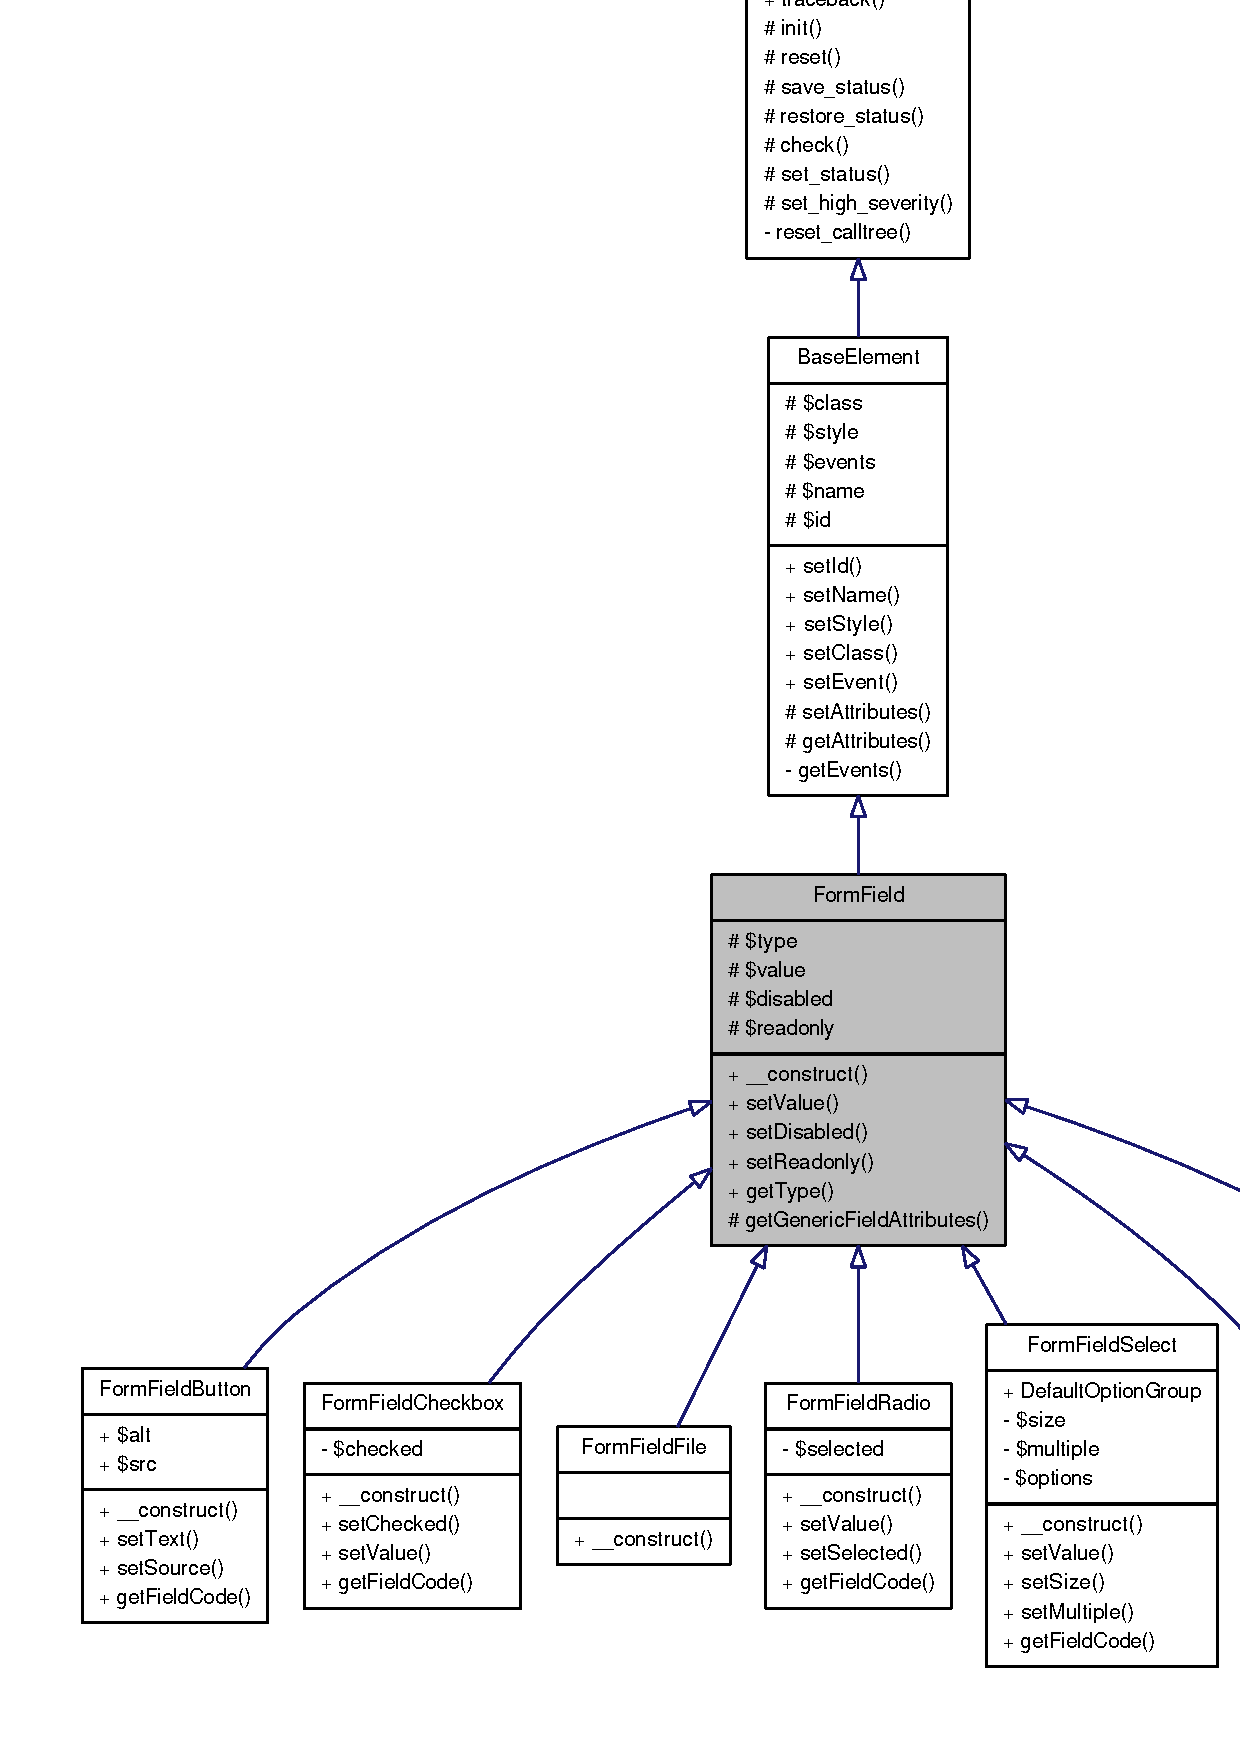
\includegraphics[width=400pt]{classFormField__inherit__graph}
\end{center}
\end{figure}


Collaboration diagram for FormField:\nopagebreak
\begin{figure}[H]
\begin{center}
\leavevmode
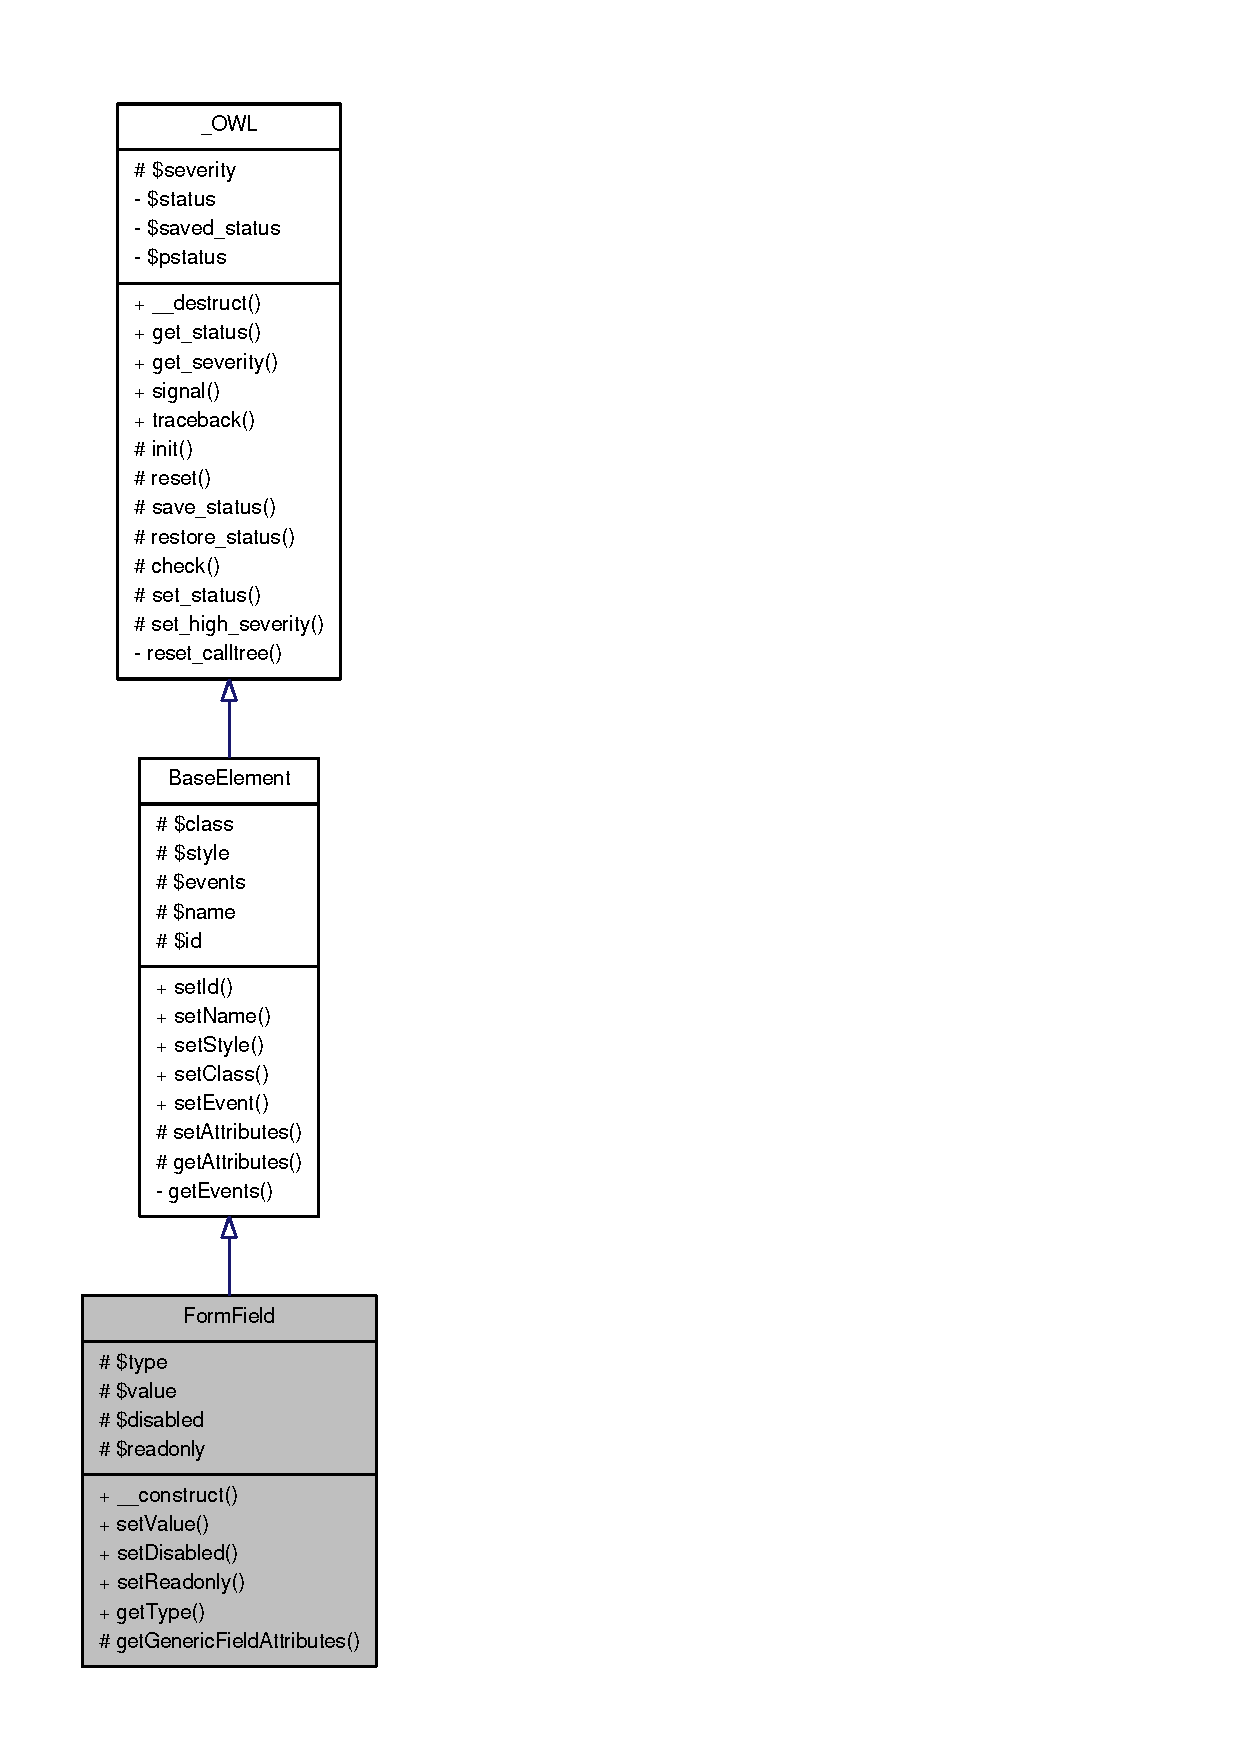
\includegraphics[height=600pt]{classFormField__coll__graph}
\end{center}
\end{figure}
\subsection*{Public Member Functions}
\begin{DoxyCompactItemize}
\item 
\hyperlink{classFormField_a0cfe713ce28a6a0cb53476ed463e1f01}{\_\-\_\-construct} ()
\item 
\hyperlink{classFormField_a465ff61e290d82be96bb793c3a14b3e7}{setValue} (\$\_\-value)
\item 
\hyperlink{classFormField_a9fa2c828eaf98154edfaa2e755657117}{setDisabled} (\$\_\-value=true)
\item 
\hyperlink{classFormField_a6eabbb35d24b1698ea25b66ddfd88a64}{setReadonly} (\$\_\-value=true)
\item 
\hyperlink{classFormField_a1f64b737bccb6b2827f8c5665b9920c7}{getType} ()
\item 
\hyperlink{classBaseElement_a0c1ce3d1684ecb78960cf7a97278494e}{setId} (\$\_\-value)
\item 
\hyperlink{classBaseElement_a39bafb3609d10048920c20242c2a04c5}{setName} (\$\_\-value)
\item 
\hyperlink{classBaseElement_a6b2b9ff69f6e92db82f91d9c55cda697}{setStyle} (\$\_\-value)
\item 
\hyperlink{classBaseElement_af6597b30fa9798878f6290271043dfa2}{setClass} (\$\_\-value)
\item 
\hyperlink{classBaseElement_ad5789f45f16aaa144716ee8558069c31}{setEvent} (\$\_\-event, \$\_\-action, \$\_\-add=false)
\item 
\hyperlink{class__OWL_a99ec771fa2c5c279f80152cc09e489a8}{get\_\-status} ()
\item 
\hyperlink{class__OWL_adf9509ef96858be7bdd9414c5ef129aa}{get\_\-severity} (\$status=null)
\item 
\hyperlink{class__OWL_a51ba4a16409acf2a2f61f286939091a5}{signal} (\$level=\hyperlink{owl_8severitycodes_8php_a139328861128689f2f4def6a399d9057}{OWL\_\-INFO}, \&\$text=false)
\item 
\hyperlink{class__OWL_aa29547995d6741b7d2b90c1d4ea99a13}{traceback} (\&\$text=false, \$depth=0)
\end{DoxyCompactItemize}
\subsection*{Protected Member Functions}
\begin{DoxyCompactItemize}
\item 
\hyperlink{classFormField_a9f9d136ba8b4a793f22370aff43d592d}{getGenericFieldAttributes} (\$\_\-ignore=array())
\item 
\hyperlink{classBaseElement_aa623b042d23a5b77add8b3c452ec5855}{setAttributes} (\$\_\-attribs)
\item 
\hyperlink{classBaseElement_ae8237038633fc53db818f36da1940297}{getAttributes} (\$\_\-ignore=array())
\item 
\hyperlink{class__OWL_ae0ef3ded56e8a6b34b6461e5a721cd3e}{init} ()
\item 
\hyperlink{class__OWL_a2f2a042bcf31965194c03033df0edc9b}{reset} ()
\item 
\hyperlink{class__OWL_a9e49b9c76fbc021b244c6915ea536d71}{save\_\-status} ()
\item 
\hyperlink{class__OWL_a465eeaf40edd9f9c848841700c32ce55}{restore\_\-status} ()
\item 
\hyperlink{class__OWL_ad6f4f6946f40199dd0333cf219fa500e}{check} (\&\$object, \$level)
\item 
\hyperlink{class__OWL_aea912d0ede9b3c2a69b79072d94d4787}{set\_\-status} (\$status, \$params=array())
\item 
\hyperlink{class__OWL_a576829692a3b66e3d518853bf43abae3}{set\_\-high\_\-severity} (\&\$object=null)
\end{DoxyCompactItemize}
\subsection*{Protected Attributes}
\begin{DoxyCompactItemize}
\item 
\hyperlink{classFormField_a37bed21a1891e95be0e4a697e45ba51b}{\$type}
\item 
\hyperlink{classFormField_a3c01e89834248eec8e2f145fbcfa0fbc}{\$value}
\item 
\hyperlink{classFormField_ab6f1907061890290e32cb2befc0a5f50}{\$disabled}
\item 
\hyperlink{classFormField_a78ba5d4b9127e75e8ccf86f397b5d9ac}{\$readonly}
\item 
\hyperlink{classBaseElement_a99976a8e967db92e7800309f359b0803}{\$class} = ''
\item 
\hyperlink{classBaseElement_a429a3d642dd95f30e1059ef29564b87d}{\$style} = ''
\item 
\hyperlink{classBaseElement_a02cebe45d277b4ff8f29db08bad371ba}{\$events} = array()
\item 
\hyperlink{classBaseElement_a30b8cff187a9de659a70daf287d66f45}{\$name} = ''
\item 
\hyperlink{classBaseElement_a11b6989c43b53869a09f5ce65aa55b45}{\$id} = ''
\item 
\hyperlink{class__OWL_ad26b40a9dbbacb33e299b17826f8327c}{\$severity}
\end{DoxyCompactItemize}


\subsection{Detailed Description}
Formfield. Abstract base class for Formfield elements \begin{DoxyAuthor}{Author}
Oscar van Eijk, Oveas Functionality Provider 
\end{DoxyAuthor}
\begin{DoxyVersion}{Version}
Oct 19, 2010 -\/-\/ O van Eijk -\/-\/ initial version 
\end{DoxyVersion}


\subsection{Constructor \& Destructor Documentation}
\index{FormField@{FormField}!\_\-\_\-construct@{\_\-\_\-construct}}
\index{\_\-\_\-construct@{\_\-\_\-construct}!FormField@{FormField}}
\subsubsection[{\_\-\_\-construct}]{\setlength{\rightskip}{0pt plus 5cm}FormField::\_\-\_\-construct (
\begin{DoxyParamCaption}
{}
\end{DoxyParamCaption}
)}\label{classFormField_a0cfe713ce28a6a0cb53476ed463e1f01}
Class constructor; 

Reimplemented in \hyperlink{classFormFieldCheckbox_a9ea37cd03013e361f11680049c1a0097}{FormFieldCheckbox}, \hyperlink{classFormFieldFile_a2e19b30454dd3ed054772868bf6eebad}{FormFieldFile}, \hyperlink{classFormFieldRadio_ae82224cf68e3513e29923c24f42eb06d}{FormFieldRadio}, \hyperlink{classFormFieldSelect_a32c59192be8c316fb2f7e1edde8f0a98}{FormFieldSelect}, and \hyperlink{classFormFieldTextarea_a65e5d308db60f1ca0d08085d09dea8bc}{FormFieldTextarea}.



References \_\-OWL::init().



Referenced by FormFieldText::\_\-\_\-construct(), and FormFieldButton::\_\-\_\-construct().



\subsection{Member Function Documentation}
\index{FormField@{FormField}!check@{check}}
\index{check@{check}!FormField@{FormField}}
\subsubsection[{check}]{\setlength{\rightskip}{0pt plus 5cm}\_\-OWL::check (
\begin{DoxyParamCaption}
\item[{\&\$}]{ object, }
\item[{\$}]{ level}
\end{DoxyParamCaption}
)\hspace{0.3cm}{\ttfamily  \mbox{[}protected, inherited\mbox{]}}}\label{class__OWL_ad6f4f6946f40199dd0333cf219fa500e}
This is a helper function for lazy developers. Some checks have to be made quite often, this is a kinda macro to handle that. It compares the own severity level with that of a given object. If the highest level is above a given max, a traceback and reset are performed.


\begin{DoxyParams}{Parameters}
\item[\mbox{\tt[in]} {\em \$object}]Pointer to an object to check against \item[\mbox{\tt[in]} {\em \$level}]The maximum severity level \end{DoxyParams}
\begin{DoxyReturn}{Returns}
True if the severity level was correct ( below the max), otherwise false 
\end{DoxyReturn}


References \_\-OWL::reset(), \_\-OWL::set\_\-high\_\-severity(), and \_\-OWL::traceback().



Referenced by SessionHandler::write().

\index{FormField@{FormField}!get\_\-severity@{get\_\-severity}}
\index{get\_\-severity@{get\_\-severity}!FormField@{FormField}}
\subsubsection[{get\_\-severity}]{\setlength{\rightskip}{0pt plus 5cm}\_\-OWL::get\_\-severity (
\begin{DoxyParamCaption}
\item[{\$}]{ status = {\ttfamily null}}
\end{DoxyParamCaption}
)\hspace{0.3cm}{\ttfamily  \mbox{[}inherited\mbox{]}}}\label{class__OWL_adf9509ef96858be7bdd9414c5ef129aa}
Get the current object severity level.


\begin{DoxyParams}{Parameters}
\item[\mbox{\tt[in]} {\em \$status}]An optional parameter to check an other status code i.s.o the object's current status. \end{DoxyParams}
\begin{DoxyReturn}{Returns}
Status severity level 
\end{DoxyReturn}


References \_\-OWL::\$status.



Referenced by LogHandler::compose\_\-message(), LogHandler::log(), and DataHandler::set\_\-key().

\index{FormField@{FormField}!get\_\-status@{get\_\-status}}
\index{get\_\-status@{get\_\-status}!FormField@{FormField}}
\subsubsection[{get\_\-status}]{\setlength{\rightskip}{0pt plus 5cm}\_\-OWL::get\_\-status (
\begin{DoxyParamCaption}
{}
\end{DoxyParamCaption}
)\hspace{0.3cm}{\ttfamily  \mbox{[}final, inherited\mbox{]}}}\label{class__OWL_a99ec771fa2c5c279f80152cc09e489a8}
Get the current object status.

\begin{DoxyReturn}{Returns}
Object's status code 
\end{DoxyReturn}


Referenced by SchemeHandler::compare().

\index{FormField@{FormField}!getAttributes@{getAttributes}}
\index{getAttributes@{getAttributes}!FormField@{FormField}}
\subsubsection[{getAttributes}]{\setlength{\rightskip}{0pt plus 5cm}BaseElement::getAttributes (
\begin{DoxyParamCaption}
\item[{\$}]{ \_\-ignore = {\ttfamily array()}}
\end{DoxyParamCaption}
)\hspace{0.3cm}{\ttfamily  \mbox{[}protected, inherited\mbox{]}}}\label{classBaseElement_ae8237038633fc53db818f36da1940297}
Return the general element attributes that are set 
\begin{DoxyParams}{Parameters}
\item[\mbox{\tt[in]} {\em \$\_\-ignore}]Array with attributes names that should be ignored \end{DoxyParams}
\begin{DoxyReturn}{Returns}
string attributes in HTML format (' fld=\char`\"{}value\char`\"{}...) 
\end{DoxyReturn}


References BaseElement::getEvents().



Referenced by getGenericFieldAttributes(), Table::getTable(), Tablecell::getTablecell(), Tablerow::getTablerow(), and Form::openForm().

\index{FormField@{FormField}!getGenericFieldAttributes@{getGenericFieldAttributes}}
\index{getGenericFieldAttributes@{getGenericFieldAttributes}!FormField@{FormField}}
\subsubsection[{getGenericFieldAttributes}]{\setlength{\rightskip}{0pt plus 5cm}FormField::getGenericFieldAttributes (
\begin{DoxyParamCaption}
\item[{\$}]{ \_\-ignore = {\ttfamily array()}}
\end{DoxyParamCaption}
)\hspace{0.3cm}{\ttfamily  \mbox{[}protected\mbox{]}}}\label{classFormField_a9f9d136ba8b4a793f22370aff43d592d}
Return the attributes for an HTML formfield in the \char`\"{} attrib='value' \mbox{[}...\mbox{]}\char`\"{} format


\begin{DoxyParams}{Parameters}
\item[\mbox{\tt[in]} {\em \$\_\-ignore}]Array with attributes names that should be ignored, e.g. for a textarea, the value is not returned as an attribute. \end{DoxyParams}
\begin{DoxyReturn}{Returns}
Textstring with the HTML code 
\end{DoxyReturn}


References BaseElement::getAttributes().



Referenced by FormFieldTextarea::getFieldCode(), FormFieldText::getFieldCode(), FormFieldSelect::getFieldCode(), FormFieldRadio::getFieldCode(), FormFieldCheckbox::getFieldCode(), and FormFieldButton::getFieldCode().

\index{FormField@{FormField}!getType@{getType}}
\index{getType@{getType}!FormField@{FormField}}
\subsubsection[{getType}]{\setlength{\rightskip}{0pt plus 5cm}FormField::getType (
\begin{DoxyParamCaption}
{}
\end{DoxyParamCaption}
)}\label{classFormField_a1f64b737bccb6b2827f8c5665b9920c7}
Give the field type \begin{DoxyReturn}{Returns}
Field type 
\end{DoxyReturn}
\index{FormField@{FormField}!init@{init}}
\index{init@{init}!FormField@{FormField}}
\subsubsection[{init}]{\setlength{\rightskip}{0pt plus 5cm}\_\-OWL::init (
\begin{DoxyParamCaption}
{}
\end{DoxyParamCaption}
)\hspace{0.3cm}{\ttfamily  \mbox{[}protected, inherited\mbox{]}}}\label{class__OWL_ae0ef3ded56e8a6b34b6461e5a721cd3e}
This function should be called by all constuctors. It initializes the general characteristics. Status is 'warning' by default, it's up to the contructor to set a proper status; if it's still 'warning', this $\ast$might$\ast$ indicate something went wrong. 

References OWL::factory().



Referenced by Tablerow::\_\-\_\-construct(), Tablecell::\_\-\_\-construct(), Table::\_\-\_\-construct(), \_\-\_\-construct(), UserHandler::\_\-\_\-construct(), SessionHandler::\_\-\_\-construct(), SchemeHandler::\_\-\_\-construct(), LogHandler::\_\-\_\-construct(), ImageHandler::\_\-\_\-construct(), FormHandler::\_\-\_\-construct(), FileHandler::\_\-\_\-construct(), DbHandler::\_\-\_\-construct(), OWL::\_\-\_\-construct(), Form::\_\-\_\-construct(), Dispatcher::\_\-\_\-construct(), and DataHandler::DataHandler().

\index{FormField@{FormField}!reset@{reset}}
\index{reset@{reset}!FormField@{FormField}}
\subsubsection[{reset}]{\setlength{\rightskip}{0pt plus 5cm}\_\-OWL::reset (
\begin{DoxyParamCaption}
{}
\end{DoxyParamCaption}
)\hspace{0.3cm}{\ttfamily  \mbox{[}protected, inherited\mbox{]}}}\label{class__OWL_a2f2a042bcf31965194c03033df0edc9b}
General reset function for all objects. Should be called after each non-\/fatal error 

Reimplemented in \hyperlink{classDbHandler_a9982df4830f05803935bb31bac7fae3d}{DbHandler}, and \hyperlink{classSchemeHandler_aa25feb4a70d67b3d571904be4b2f50bc}{SchemeHandler}.



References \_\-OWL::reset\_\-calltree().



Referenced by \_\-OWL::check(), SessionHandler::read(), DataHandler::reset(), and \_\-OWL::set\_\-status().

\index{FormField@{FormField}!restore\_\-status@{restore\_\-status}}
\index{restore\_\-status@{restore\_\-status}!FormField@{FormField}}
\subsubsection[{restore\_\-status}]{\setlength{\rightskip}{0pt plus 5cm}\_\-OWL::restore\_\-status (
\begin{DoxyParamCaption}
{}
\end{DoxyParamCaption}
)\hspace{0.3cm}{\ttfamily  \mbox{[}protected, inherited\mbox{]}}}\label{class__OWL_a465eeaf40edd9f9c848841700c32ce55}
Restore the previously saved status object and destroy the copy 

References \_\-OWL::set\_\-status().



Referenced by UserHandler::logout().

\index{FormField@{FormField}!save\_\-status@{save\_\-status}}
\index{save\_\-status@{save\_\-status}!FormField@{FormField}}
\subsubsection[{save\_\-status}]{\setlength{\rightskip}{0pt plus 5cm}\_\-OWL::save\_\-status (
\begin{DoxyParamCaption}
{}
\end{DoxyParamCaption}
)\hspace{0.3cm}{\ttfamily  \mbox{[}protected, inherited\mbox{]}}}\label{class__OWL_a9e49b9c76fbc021b244c6915ea536d71}
Create a copy of the status object 

Referenced by UserHandler::logout().

\index{FormField@{FormField}!set\_\-high\_\-severity@{set\_\-high\_\-severity}}
\index{set\_\-high\_\-severity@{set\_\-high\_\-severity}!FormField@{FormField}}
\subsubsection[{set\_\-high\_\-severity}]{\setlength{\rightskip}{0pt plus 5cm}\_\-OWL::set\_\-high\_\-severity (
\begin{DoxyParamCaption}
\item[{\&\$}]{ object = {\ttfamily null}}
\end{DoxyParamCaption}
)\hspace{0.3cm}{\ttfamily  \mbox{[}protected, inherited\mbox{]}}}\label{class__OWL_a576829692a3b66e3d518853bf43abae3}
Compare the severity level of the current object with a given one and set my statuspointer to the object with the highest level. 

Referenced by \_\-OWL::check(), DataHandler::db(), DataHandler::prepare(), and SessionHandler::read().

\index{FormField@{FormField}!set\_\-status@{set\_\-status}}
\index{set\_\-status@{set\_\-status}!FormField@{FormField}}
\subsubsection[{set\_\-status}]{\setlength{\rightskip}{0pt plus 5cm}\_\-OWL::set\_\-status (
\begin{DoxyParamCaption}
\item[{\$}]{ status, }
\item[{\$}]{ params = {\ttfamily array~()}}
\end{DoxyParamCaption}
)\hspace{0.3cm}{\ttfamily  \mbox{[}final, protected, inherited\mbox{]}}}\label{class__OWL_aea912d0ede9b3c2a69b79072d94d4787}
Set the current object status to the specified value.


\begin{DoxyParams}{Parameters}
\item[\mbox{\tt[in]} {\em \$status}]\hyperlink{classOWL}{OWL} status code \item[\mbox{\tt[in]} {\em \$params}]\end{DoxyParams}


References \$GLOBALS, \_\-OWL::\$status, ConfigHandler::get(), Register::get\_\-code(), \_\-OWL::reset(), and \_\-OWL::signal().



Referenced by UserHandler::\_\-\_\-construct(), SessionHandler::\_\-\_\-construct(), SchemeHandler::\_\-\_\-construct(), ImageHandler::\_\-\_\-construct(), FormHandler::\_\-\_\-construct(), FileHandler::\_\-\_\-construct(), DbHandler::\_\-\_\-construct(), Form::\_\-\_\-construct(), Form::addField(), SchemeHandler::alter\_\-scheme(), FileHandler::close(), DbHandler::connect(), DbHandler::create(), SchemeHandler::create\_\-scheme(), DataHandler::DataHandler(), SchemeHandler::define\_\-index(), SchemeHandler::define\_\-scheme(), Dispatcher::dispatch(), FormHandler::get(), DataHandler::get(), SchemeHandler::get\_\-table\_\-columns(), SchemeHandler::get\_\-table\_\-indexes(), UserHandler::login(), FileHandler::open(), DbHandler::open(), LogHandler::open\_\-logfile(), DataHandler::prepare(), DbHandler::prepare\_\-delete(), DbHandler::prepare\_\-insert(), DbHandler::prepare\_\-read(), DbHandler::prepare\_\-update(), DbHandler::read(), FileHandler::read\_\-line(), UserHandler::read\_\-userdata(), \_\-OWL::restore\_\-status(), SchemeHandler::scheme(), FormHandler::set(), DataHandler::set(), DataHandler::set\_\-join(), DataHandler::set\_\-key(), BaseElement::setAttributes(), Form::setEncoding(), Form::setFieldAttributes(), FormFieldText::setMaxsize(), Form::setMethod(), FormFieldRadio::setSelected(), FormFieldText::setSize(), FormFieldSelect::setSize(), FormFieldSelect::setValue(), FormFieldRadio::setValue(), Form::showField(), SchemeHandler::table\_\-description(), SchemeHandler::validate\_\-scheme(), and DbHandler::write().

\index{FormField@{FormField}!setAttributes@{setAttributes}}
\index{setAttributes@{setAttributes}!FormField@{FormField}}
\subsubsection[{setAttributes}]{\setlength{\rightskip}{0pt plus 5cm}BaseElement::setAttributes (
\begin{DoxyParamCaption}
\item[{\$}]{ \_\-attribs}
\end{DoxyParamCaption}
)\hspace{0.3cm}{\ttfamily  \mbox{[}protected, inherited\mbox{]}}}\label{classBaseElement_aa623b042d23a5b77add8b3c452ec5855}
Set the attributes of the DOM element by calling the 'set$<$Attrib$>$' method for this class. 
\begin{DoxyParams}{Parameters}
\item[\mbox{\tt[in]} {\em \$\_\-attribs}]Array with attributes in the format attrib=$>$value \end{DoxyParams}
\begin{DoxyReturn}{Returns}
Severity level. The status increased when a set$<$Attrib\&gt method does not exist. 
\end{DoxyReturn}


Reimplemented in \hyperlink{classTablecell_a91a8264df222cc44b77ceaf7282a400e}{Tablecell}, and \hyperlink{classTablerow_aece4cad0834c299d7e03030e945aea3a}{Tablerow}.



References \_\-OWL::set\_\-status().



Referenced by Table::\_\-\_\-construct().

\index{FormField@{FormField}!setClass@{setClass}}
\index{setClass@{setClass}!FormField@{FormField}}
\subsubsection[{setClass}]{\setlength{\rightskip}{0pt plus 5cm}BaseElement::setClass (
\begin{DoxyParamCaption}
\item[{\$}]{ \_\-value}
\end{DoxyParamCaption}
)\hspace{0.3cm}{\ttfamily  \mbox{[}inherited\mbox{]}}}\label{classBaseElement_af6597b30fa9798878f6290271043dfa2}
Set the element Class 
\begin{DoxyParams}{Parameters}
\item[\mbox{\tt[in]} {\em \$\_\-value}]Class name \end{DoxyParams}
\index{FormField@{FormField}!setDisabled@{setDisabled}}
\index{setDisabled@{setDisabled}!FormField@{FormField}}
\subsubsection[{setDisabled}]{\setlength{\rightskip}{0pt plus 5cm}FormField::setDisabled (
\begin{DoxyParamCaption}
\item[{\$}]{ \_\-value = {\ttfamily true}}
\end{DoxyParamCaption}
)}\label{classFormField_a9fa2c828eaf98154edfaa2e755657117}
Set the Disabled boolean 
\begin{DoxyParams}{Parameters}
\item[\mbox{\tt[in]} {\em \$\_\-value}]Value indicating true (default) or false \end{DoxyParams}
\index{FormField@{FormField}!setEvent@{setEvent}}
\index{setEvent@{setEvent}!FormField@{FormField}}
\subsubsection[{setEvent}]{\setlength{\rightskip}{0pt plus 5cm}BaseElement::setEvent (
\begin{DoxyParamCaption}
\item[{\$}]{ \_\-event, }
\item[{\$}]{ \_\-action, }
\item[{\$}]{ \_\-add = {\ttfamily false}}
\end{DoxyParamCaption}
)\hspace{0.3cm}{\ttfamily  \mbox{[}inherited\mbox{]}}}\label{classBaseElement_ad5789f45f16aaa144716ee8558069c31}
Add an event to the events array 
\begin{DoxyParams}{Parameters}
\item[\mbox{\tt[in]} {\em \$\_\-event}]Javascript event name (onXxx) \item[\mbox{\tt[in]} {\em \$\_\-action}]Javascript function or code \item[\mbox{\tt[in]} {\em \$\_\-add}]Boolean; when true, the action will be added if the event name already exists. Default is false; overwrite the action for this event. \end{DoxyParams}
\index{FormField@{FormField}!setId@{setId}}
\index{setId@{setId}!FormField@{FormField}}
\subsubsection[{setId}]{\setlength{\rightskip}{0pt plus 5cm}BaseElement::setId (
\begin{DoxyParamCaption}
\item[{\$}]{ \_\-value}
\end{DoxyParamCaption}
)\hspace{0.3cm}{\ttfamily  \mbox{[}inherited\mbox{]}}}\label{classBaseElement_a0c1ce3d1684ecb78960cf7a97278494e}
Set the element ID 
\begin{DoxyParams}{Parameters}
\item[\mbox{\tt[in]} {\em \$\_\-value}]Identification \end{DoxyParams}
\index{FormField@{FormField}!setName@{setName}}
\index{setName@{setName}!FormField@{FormField}}
\subsubsection[{setName}]{\setlength{\rightskip}{0pt plus 5cm}BaseElement::setName (
\begin{DoxyParamCaption}
\item[{\$}]{ \_\-value}
\end{DoxyParamCaption}
)\hspace{0.3cm}{\ttfamily  \mbox{[}inherited\mbox{]}}}\label{classBaseElement_a39bafb3609d10048920c20242c2a04c5}
Set the element name 
\begin{DoxyParams}{Parameters}
\item[\mbox{\tt[in]} {\em \$\_\-value}]Element name \end{DoxyParams}
\index{FormField@{FormField}!setReadonly@{setReadonly}}
\index{setReadonly@{setReadonly}!FormField@{FormField}}
\subsubsection[{setReadonly}]{\setlength{\rightskip}{0pt plus 5cm}FormField::setReadonly (
\begin{DoxyParamCaption}
\item[{\$}]{ \_\-value = {\ttfamily true}}
\end{DoxyParamCaption}
)}\label{classFormField_a6eabbb35d24b1698ea25b66ddfd88a64}
Set the Readonly boolean 
\begin{DoxyParams}{Parameters}
\item[\mbox{\tt[in]} {\em \$\_\-value}]Value indicating true (default) or false \end{DoxyParams}
\index{FormField@{FormField}!setStyle@{setStyle}}
\index{setStyle@{setStyle}!FormField@{FormField}}
\subsubsection[{setStyle}]{\setlength{\rightskip}{0pt plus 5cm}BaseElement::setStyle (
\begin{DoxyParamCaption}
\item[{\$}]{ \_\-value}
\end{DoxyParamCaption}
)\hspace{0.3cm}{\ttfamily  \mbox{[}inherited\mbox{]}}}\label{classBaseElement_a6b2b9ff69f6e92db82f91d9c55cda697}
Set the element style 
\begin{DoxyParams}{Parameters}
\item[\mbox{\tt[in]} {\em \$\_\-value}]Element style \end{DoxyParams}
\index{FormField@{FormField}!setValue@{setValue}}
\index{setValue@{setValue}!FormField@{FormField}}
\subsubsection[{setValue}]{\setlength{\rightskip}{0pt plus 5cm}FormField::setValue (
\begin{DoxyParamCaption}
\item[{\$}]{ \_\-value}
\end{DoxyParamCaption}
)}\label{classFormField_a465ff61e290d82be96bb793c3a14b3e7}
Set the field value 
\begin{DoxyParams}{Parameters}
\item[\mbox{\tt[in]} {\em \$\_\-value}]Field value \end{DoxyParams}


Reimplemented in \hyperlink{classFormFieldCheckbox_a787abee157599c389a18e0810f69fed5}{FormFieldCheckbox}, \hyperlink{classFormFieldRadio_aab105e92866fd80890d3254f51a2e4ca}{FormFieldRadio}, and \hyperlink{classFormFieldSelect_ae69f5b352df63796c048dca6a2de7544}{FormFieldSelect}.

\index{FormField@{FormField}!signal@{signal}}
\index{signal@{signal}!FormField@{FormField}}
\subsubsection[{signal}]{\setlength{\rightskip}{0pt plus 5cm}\_\-OWL::signal (
\begin{DoxyParamCaption}
\item[{\$}]{ level = {\ttfamily {\bf OWL\_\-INFO}}, }
\item[{\&\$}]{ text = {\ttfamily false}}
\end{DoxyParamCaption}
)\hspace{0.3cm}{\ttfamily  \mbox{[}inherited\mbox{]}}}\label{class__OWL_a51ba4a16409acf2a2f61f286939091a5}
Display the message for the current object status


\begin{DoxyParams}{Parameters}
\item[\mbox{\tt[in]} {\em \$level}]An optional severity level; message will only be displayed when it is at least of this level. \item[\mbox{\tt[out]} {\em \$text}]If this parameter is given, the message text is returned in this string instead of echood. \end{DoxyParams}
\begin{DoxyReturn}{Returns}
The severity level for this object 
\end{DoxyReturn}


References ConfigHandler::get().



Referenced by \_\-OWL::set\_\-status(), and \_\-OWL::traceback().

\index{FormField@{FormField}!traceback@{traceback}}
\index{traceback@{traceback}!FormField@{FormField}}
\subsubsection[{traceback}]{\setlength{\rightskip}{0pt plus 5cm}\_\-OWL::traceback (
\begin{DoxyParamCaption}
\item[{\&\$}]{ text = {\ttfamily false}, }
\item[{\$}]{ depth = {\ttfamily 0}}
\end{DoxyParamCaption}
)\hspace{0.3cm}{\ttfamily  \mbox{[}inherited\mbox{]}}}\label{class__OWL_aa29547995d6741b7d2b90c1d4ea99a13}
If somehwere in the nested calls an error occured, we can traceback the original failing object with this function and signal the message.


\begin{DoxyParams}{Parameters}
\item[\mbox{\tt[out]} {\em \$text}]Optional variable in which the message text can be stored. If not given, the text will be written to standard output \item[\mbox{\tt[in]} {\em \$depth}]This paramater should be initially empty. It calculates the depth in recursive calls. \end{DoxyParams}
\begin{DoxyReturn}{Returns}
Severity code of the failing object 
\end{DoxyReturn}


References \_\-OWL::signal().



Referenced by \_\-OWL::check(), UserHandler::login(), and SessionHandler::read().



\subsection{Member Data Documentation}
\index{FormField@{FormField}!\$class@{\$class}}
\index{\$class@{\$class}!FormField@{FormField}}
\subsubsection[{\$class}]{\setlength{\rightskip}{0pt plus 5cm}BaseElement::\$class = ''\hspace{0.3cm}{\ttfamily  \mbox{[}protected, inherited\mbox{]}}}\label{classBaseElement_a99976a8e967db92e7800309f359b0803}
Class specification \index{FormField@{FormField}!\$disabled@{\$disabled}}
\index{\$disabled@{\$disabled}!FormField@{FormField}}
\subsubsection[{\$disabled}]{\setlength{\rightskip}{0pt plus 5cm}FormField::\$disabled\hspace{0.3cm}{\ttfamily  \mbox{[}protected\mbox{]}}}\label{classFormField_ab6f1907061890290e32cb2befc0a5f50}
Boolean indicating a disabled field when true \index{FormField@{FormField}!\$events@{\$events}}
\index{\$events@{\$events}!FormField@{FormField}}
\subsubsection[{\$events}]{\setlength{\rightskip}{0pt plus 5cm}BaseElement::\$events = array()\hspace{0.3cm}{\ttfamily  \mbox{[}protected, inherited\mbox{]}}}\label{classBaseElement_a02cebe45d277b4ff8f29db08bad371ba}
Array with javascript events 

Referenced by Form::setFieldEvents().

\index{FormField@{FormField}!\$id@{\$id}}
\index{\$id@{\$id}!FormField@{FormField}}
\subsubsection[{\$id}]{\setlength{\rightskip}{0pt plus 5cm}BaseElement::\$id = ''\hspace{0.3cm}{\ttfamily  \mbox{[}protected, inherited\mbox{]}}}\label{classBaseElement_a11b6989c43b53869a09f5ce65aa55b45}
Element ID \index{FormField@{FormField}!\$name@{\$name}}
\index{\$name@{\$name}!FormField@{FormField}}
\subsubsection[{\$name}]{\setlength{\rightskip}{0pt plus 5cm}BaseElement::\$name = ''\hspace{0.3cm}{\ttfamily  \mbox{[}protected, inherited\mbox{]}}}\label{classBaseElement_a30b8cff187a9de659a70daf287d66f45}
Name of the element 

Referenced by Form::addField(), and Form::showField().

\index{FormField@{FormField}!\$readonly@{\$readonly}}
\index{\$readonly@{\$readonly}!FormField@{FormField}}
\subsubsection[{\$readonly}]{\setlength{\rightskip}{0pt plus 5cm}FormField::\$readonly\hspace{0.3cm}{\ttfamily  \mbox{[}protected\mbox{]}}}\label{classFormField_a78ba5d4b9127e75e8ccf86f397b5d9ac}
Boolean indicating a readonly field when true \index{FormField@{FormField}!\$severity@{\$severity}}
\index{\$severity@{\$severity}!FormField@{FormField}}
\subsubsection[{\$severity}]{\setlength{\rightskip}{0pt plus 5cm}\_\-OWL::\$severity\hspace{0.3cm}{\ttfamily  \mbox{[}protected, inherited\mbox{]}}}\label{class__OWL_ad26b40a9dbbacb33e299b17826f8327c}
Severity level of the current object status \index{FormField@{FormField}!\$style@{\$style}}
\index{\$style@{\$style}!FormField@{FormField}}
\subsubsection[{\$style}]{\setlength{\rightskip}{0pt plus 5cm}BaseElement::\$style = ''\hspace{0.3cm}{\ttfamily  \mbox{[}protected, inherited\mbox{]}}}\label{classBaseElement_a429a3d642dd95f30e1059ef29564b87d}
Element style \index{FormField@{FormField}!\$type@{\$type}}
\index{\$type@{\$type}!FormField@{FormField}}
\subsubsection[{\$type}]{\setlength{\rightskip}{0pt plus 5cm}FormField::\$type\hspace{0.3cm}{\ttfamily  \mbox{[}protected\mbox{]}}}\label{classFormField_a37bed21a1891e95be0e4a697e45ba51b}
Field type 

Reimplemented in \hyperlink{classFormFieldTextarea_a85348034822c70694fc8640bfcacc04d}{FormFieldTextarea}.



Referenced by FormFieldText::\_\-\_\-construct(), and FormFieldButton::\_\-\_\-construct().

\index{FormField@{FormField}!\$value@{\$value}}
\index{\$value@{\$value}!FormField@{FormField}}
\subsubsection[{\$value}]{\setlength{\rightskip}{0pt plus 5cm}FormField::\$value\hspace{0.3cm}{\ttfamily  \mbox{[}protected\mbox{]}}}\label{classFormField_a3c01e89834248eec8e2f145fbcfa0fbc}
Field value 

The documentation for this class was generated from the following file:\begin{DoxyCompactItemize}
\item 
/home/oscar/projects/owl-\/php/src/kernel/ui/\hyperlink{class_8formfield_8php}{class.formfield.php}\end{DoxyCompactItemize}

\section{FormFieldButton Class Reference}
\label{classFormFieldButton}\index{FormFieldButton@{FormFieldButton}}


Formfield.  




Inheritance diagram for FormFieldButton:\nopagebreak
\begin{figure}[H]
\begin{center}
\leavevmode
\includegraphics[width=184pt]{classFormFieldButton__inherit__graph}
\end{center}
\end{figure}


Collaboration diagram for FormFieldButton:\nopagebreak
\begin{figure}[H]
\begin{center}
\leavevmode
\includegraphics[width=184pt]{classFormFieldButton__coll__graph}
\end{center}
\end{figure}
\subsection*{Public Member Functions}
\begin{DoxyCompactItemize}
\item 
\hyperlink{classFormFieldButton_aa531597334029bd24bcaf4236d540d69}{\_\-\_\-construct} (\$type= 'button')
\item 
\hyperlink{classFormFieldButton_a792223807cd33f982ec6a5869120baab}{getFieldCode} ()
\item 
\hyperlink{classFormField_ad57e32bd53170af060e869b3b60f0ef7}{setName} (\$\_\-value)
\item 
\hyperlink{classFormField_a465ff61e290d82be96bb793c3a14b3e7}{setValue} (\$\_\-value)
\item 
\hyperlink{classFormField_a1f64b737bccb6b2827f8c5665b9920c7}{getType} ()
\end{DoxyCompactItemize}
\subsection*{Public Attributes}
\begin{DoxyCompactItemize}
\item 
\hyperlink{classFormFieldButton_afd8b16194bd066a1beaa02c450bbe4e5}{\$alt}
\item 
\hyperlink{classFormFieldButton_a9cc3c232dc78605cdff84f4784298d08}{\$src}
\end{DoxyCompactItemize}
\subsection*{Protected Member Functions}
\begin{DoxyCompactItemize}
\item 
\hyperlink{classFormField_a9f9d136ba8b4a793f22370aff43d592d}{getGenericFieldAttributes} (\$\_\-ignore=array())
\end{DoxyCompactItemize}
\subsection*{Protected Attributes}
\begin{DoxyCompactItemize}
\item 
\hyperlink{classFormField_a37bed21a1891e95be0e4a697e45ba51b}{\$type}
\item 
\hyperlink{classFormField_a23861f707bcd77bbace6300de9621746}{\$name}
\item 
\hyperlink{classFormField_a3c01e89834248eec8e2f145fbcfa0fbc}{\$value}
\item 
\hyperlink{classFormField_ab6f1907061890290e32cb2befc0a5f50}{\$disabled}
\item 
\hyperlink{classFormField_a78ba5d4b9127e75e8ccf86f397b5d9ac}{\$readonly}
\end{DoxyCompactItemize}


\subsection{Detailed Description}
Formfield. Formfield button elements \begin{DoxyAuthor}{Author}
Oscar van Eijk, Oveas Functionality Provider 
\end{DoxyAuthor}
\begin{DoxyVersion}{Version}
Oct 19, 2010 -\/-\/ O van Eijk -\/-\/ initial version 
\end{DoxyVersion}


\subsection{Constructor \& Destructor Documentation}
\index{FormFieldButton@{FormFieldButton}!\_\-\_\-construct@{\_\-\_\-construct}}
\index{\_\-\_\-construct@{\_\-\_\-construct}!FormFieldButton@{FormFieldButton}}
\subsubsection[{\_\-\_\-construct}]{\setlength{\rightskip}{0pt plus 5cm}FormFieldButton::\_\-\_\-construct (\$ {\em type} = {\ttfamily 'button'})}\label{classFormFieldButton_aa531597334029bd24bcaf4236d540d69}
Class constructor; 
\begin{DoxyParams}{Parameters}
\item[\mbox{$\leftarrow$} {\em \$type}]Element type: button (default), image, submit or reset \end{DoxyParams}


References FormField::\$type, and FormField::\_\-\_\-construct().



\subsection{Member Function Documentation}
\index{FormFieldButton@{FormFieldButton}!getFieldCode@{getFieldCode}}
\index{getFieldCode@{getFieldCode}!FormFieldButton@{FormFieldButton}}
\subsubsection[{getFieldCode}]{\setlength{\rightskip}{0pt plus 5cm}FormFieldButton::getFieldCode ()}\label{classFormFieldButton_a792223807cd33f982ec6a5869120baab}
Return the HTML code to display the form element

\begin{DoxyReturn}{Returns}
Textstring with the complete code for the form element 
\end{DoxyReturn}


References FormField::getGenericFieldAttributes().

\index{FormFieldButton@{FormFieldButton}!getGenericFieldAttributes@{getGenericFieldAttributes}}
\index{getGenericFieldAttributes@{getGenericFieldAttributes}!FormFieldButton@{FormFieldButton}}
\subsubsection[{getGenericFieldAttributes}]{\setlength{\rightskip}{0pt plus 5cm}FormField::getGenericFieldAttributes (\$ {\em \_\-ignore} = {\ttfamily array()})\hspace{0.3cm}{\ttfamily  \mbox{[}protected, inherited\mbox{]}}}\label{classFormField_a9f9d136ba8b4a793f22370aff43d592d}
Return the attributes for an HTML formfield in the \char`\"{} attrib='value' \mbox{[}...\mbox{]}\char`\"{} format


\begin{DoxyParams}{Parameters}
\item[\mbox{$\leftarrow$} {\em \$\_\-ignore}]Array with attributes names that should be ignored, e.g. for a textarea, the value is not returned as an attribute. \end{DoxyParams}
\begin{DoxyReturn}{Returns}
Textstring with the HTML code 
\end{DoxyReturn}


Referenced by FormFieldTextarea::getFieldCode(), FormFieldText::getFieldCode(), FormFieldRadio::getFieldCode(), FormFieldCheckbox::getFieldCode(), and getFieldCode().

\index{FormFieldButton@{FormFieldButton}!getType@{getType}}
\index{getType@{getType}!FormFieldButton@{FormFieldButton}}
\subsubsection[{getType}]{\setlength{\rightskip}{0pt plus 5cm}FormField::getType ()\hspace{0.3cm}{\ttfamily  \mbox{[}inherited\mbox{]}}}\label{classFormField_a1f64b737bccb6b2827f8c5665b9920c7}
Give the field type \begin{DoxyReturn}{Returns}
Field type 
\end{DoxyReturn}
\index{FormFieldButton@{FormFieldButton}!setName@{setName}}
\index{setName@{setName}!FormFieldButton@{FormFieldButton}}
\subsubsection[{setName}]{\setlength{\rightskip}{0pt plus 5cm}FormField::setName (\$ {\em \_\-value})\hspace{0.3cm}{\ttfamily  \mbox{[}inherited\mbox{]}}}\label{classFormField_ad57e32bd53170af060e869b3b60f0ef7}
Set the field name 
\begin{DoxyParams}{Parameters}
\item[\mbox{$\leftarrow$} {\em \$\_\-value}]Field name \end{DoxyParams}
\index{FormFieldButton@{FormFieldButton}!setValue@{setValue}}
\index{setValue@{setValue}!FormFieldButton@{FormFieldButton}}
\subsubsection[{setValue}]{\setlength{\rightskip}{0pt plus 5cm}FormField::setValue (\$ {\em \_\-value})\hspace{0.3cm}{\ttfamily  \mbox{[}inherited\mbox{]}}}\label{classFormField_a465ff61e290d82be96bb793c3a14b3e7}
Set the field value 
\begin{DoxyParams}{Parameters}
\item[\mbox{$\leftarrow$} {\em \$\_\-value}]Field value \end{DoxyParams}


Reimplemented in \hyperlink{classFormFieldCheckbox_a787abee157599c389a18e0810f69fed5}{FormFieldCheckbox}, \hyperlink{classFormFieldRadio_aab105e92866fd80890d3254f51a2e4ca}{FormFieldRadio}, and \hyperlink{classFormFieldSelect_ae69f5b352df63796c048dca6a2de7544}{FormFieldSelect}.



\subsection{Member Data Documentation}
\index{FormFieldButton@{FormFieldButton}!\$alt@{\$alt}}
\index{\$alt@{\$alt}!FormFieldButton@{FormFieldButton}}
\subsubsection[{\$alt}]{\setlength{\rightskip}{0pt plus 5cm}FormFieldButton::\$alt}\label{classFormFieldButton_afd8b16194bd066a1beaa02c450bbe4e5}
Alternate text (image-\/type only) \index{FormFieldButton@{FormFieldButton}!\$disabled@{\$disabled}}
\index{\$disabled@{\$disabled}!FormFieldButton@{FormFieldButton}}
\subsubsection[{\$disabled}]{\setlength{\rightskip}{0pt plus 5cm}FormField::\$disabled\hspace{0.3cm}{\ttfamily  \mbox{[}protected, inherited\mbox{]}}}\label{classFormField_ab6f1907061890290e32cb2befc0a5f50}
Boolean indicating a disabled field when true \index{FormFieldButton@{FormFieldButton}!\$name@{\$name}}
\index{\$name@{\$name}!FormFieldButton@{FormFieldButton}}
\subsubsection[{\$name}]{\setlength{\rightskip}{0pt plus 5cm}FormField::\$name\hspace{0.3cm}{\ttfamily  \mbox{[}protected, inherited\mbox{]}}}\label{classFormField_a23861f707bcd77bbace6300de9621746}
Name of the formfield \index{FormFieldButton@{FormFieldButton}!\$readonly@{\$readonly}}
\index{\$readonly@{\$readonly}!FormFieldButton@{FormFieldButton}}
\subsubsection[{\$readonly}]{\setlength{\rightskip}{0pt plus 5cm}FormField::\$readonly\hspace{0.3cm}{\ttfamily  \mbox{[}protected, inherited\mbox{]}}}\label{classFormField_a78ba5d4b9127e75e8ccf86f397b5d9ac}
Boolean indicating a readonly field when true \index{FormFieldButton@{FormFieldButton}!\$src@{\$src}}
\index{\$src@{\$src}!FormFieldButton@{FormFieldButton}}
\subsubsection[{\$src}]{\setlength{\rightskip}{0pt plus 5cm}FormFieldButton::\$src}\label{classFormFieldButton_a9cc3c232dc78605cdff84f4784298d08}
Image src (image-\/type only) \index{FormFieldButton@{FormFieldButton}!\$type@{\$type}}
\index{\$type@{\$type}!FormFieldButton@{FormFieldButton}}
\subsubsection[{\$type}]{\setlength{\rightskip}{0pt plus 5cm}FormField::\$type\hspace{0.3cm}{\ttfamily  \mbox{[}protected, inherited\mbox{]}}}\label{classFormField_a37bed21a1891e95be0e4a697e45ba51b}
Field type 

Reimplemented in \hyperlink{classFormFieldTextarea_a85348034822c70694fc8640bfcacc04d}{FormFieldTextarea}.



Referenced by FormFieldText::\_\-\_\-construct(), and \_\-\_\-construct().

\index{FormFieldButton@{FormFieldButton}!\$value@{\$value}}
\index{\$value@{\$value}!FormFieldButton@{FormFieldButton}}
\subsubsection[{\$value}]{\setlength{\rightskip}{0pt plus 5cm}FormField::\$value\hspace{0.3cm}{\ttfamily  \mbox{[}protected, inherited\mbox{]}}}\label{classFormField_a3c01e89834248eec8e2f145fbcfa0fbc}
Field value 

The documentation for this class was generated from the following file:\begin{DoxyCompactItemize}
\item 
/home/oscar/projects/owl-\/php/src/kernel/ui/\hyperlink{class_8formfield_8button_8php}{class.formfield.button.php}\end{DoxyCompactItemize}

\section{FormFieldCheckbox Class Reference}
\label{classFormFieldCheckbox}\index{FormFieldCheckbox@{FormFieldCheckbox}}


Formfield.  




Inheritance diagram for FormFieldCheckbox:\nopagebreak
\begin{figure}[H]
\begin{center}
\leavevmode
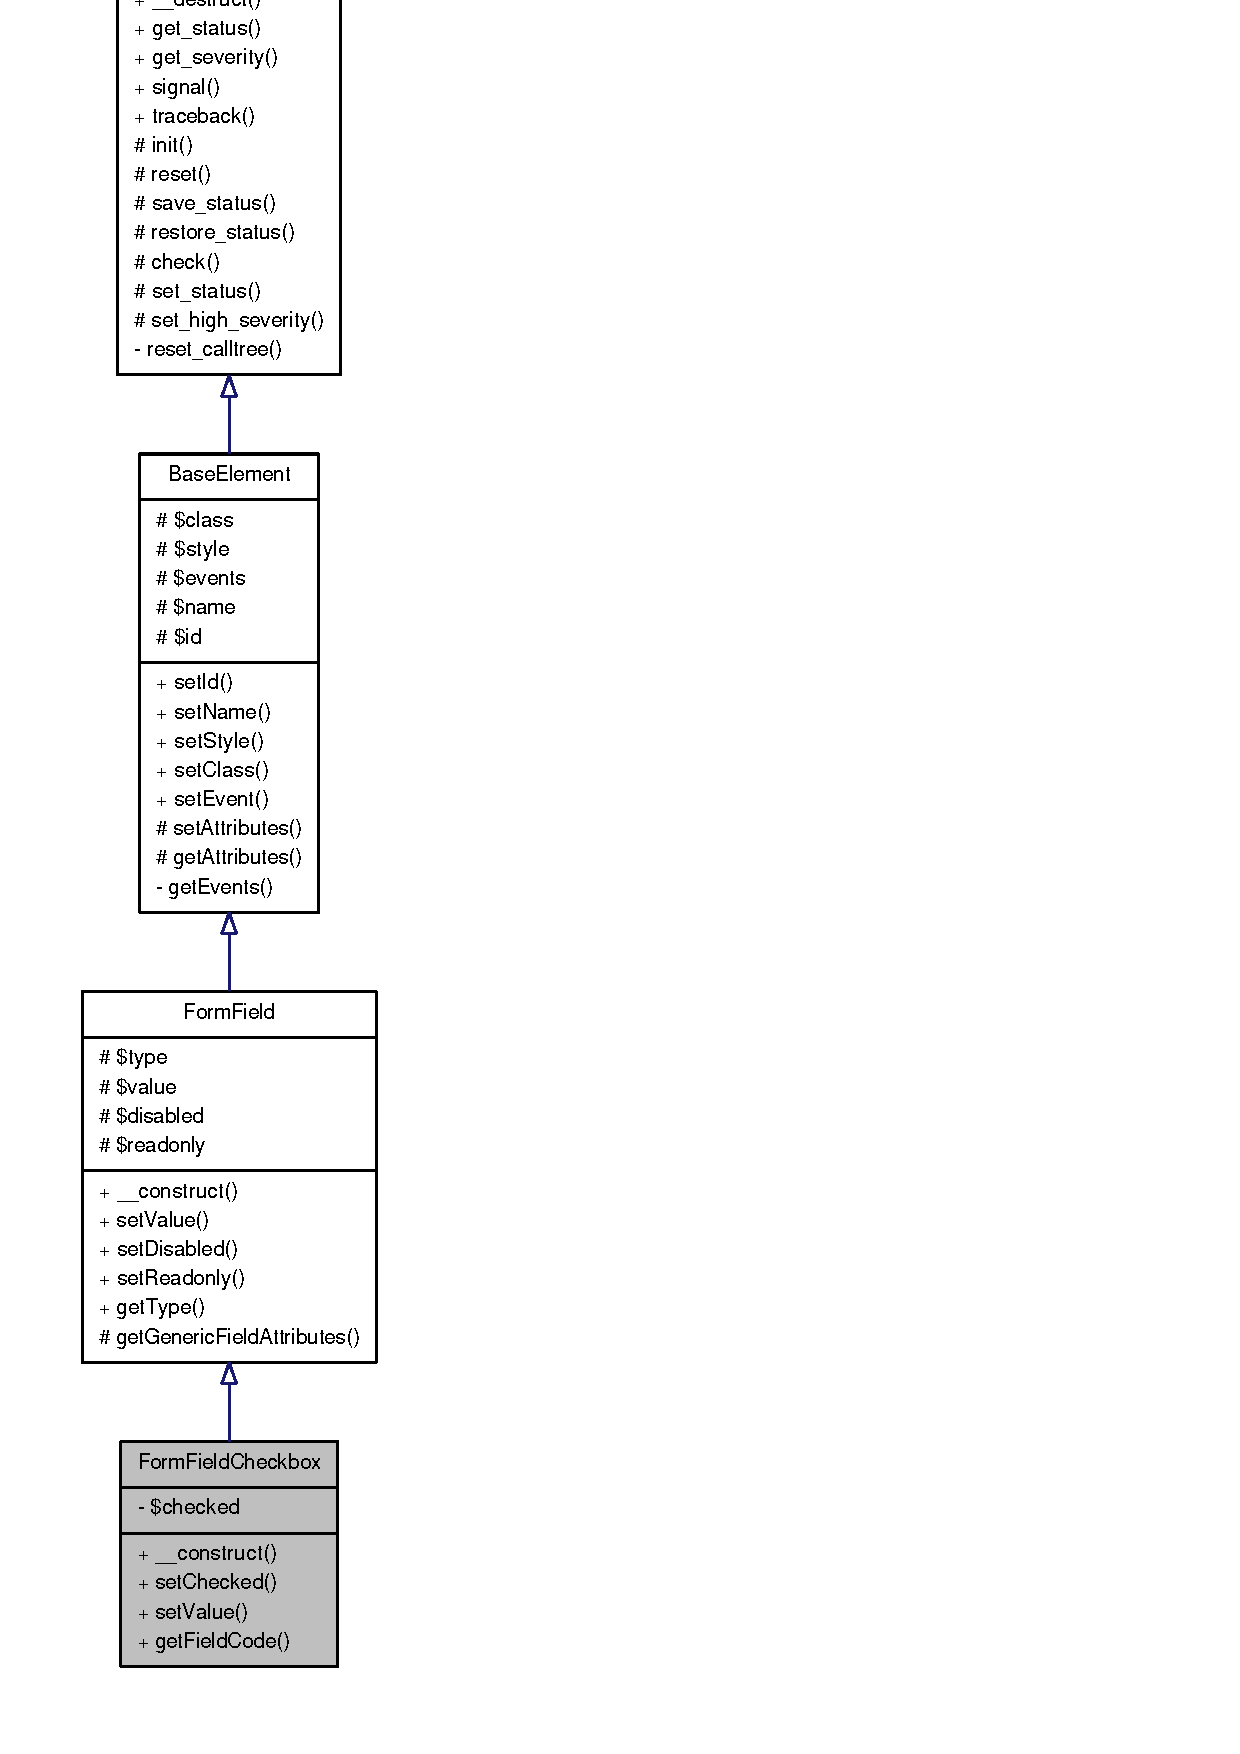
\includegraphics[height=600pt]{classFormFieldCheckbox__inherit__graph}
\end{center}
\end{figure}


Collaboration diagram for FormFieldCheckbox:\nopagebreak
\begin{figure}[H]
\begin{center}
\leavevmode
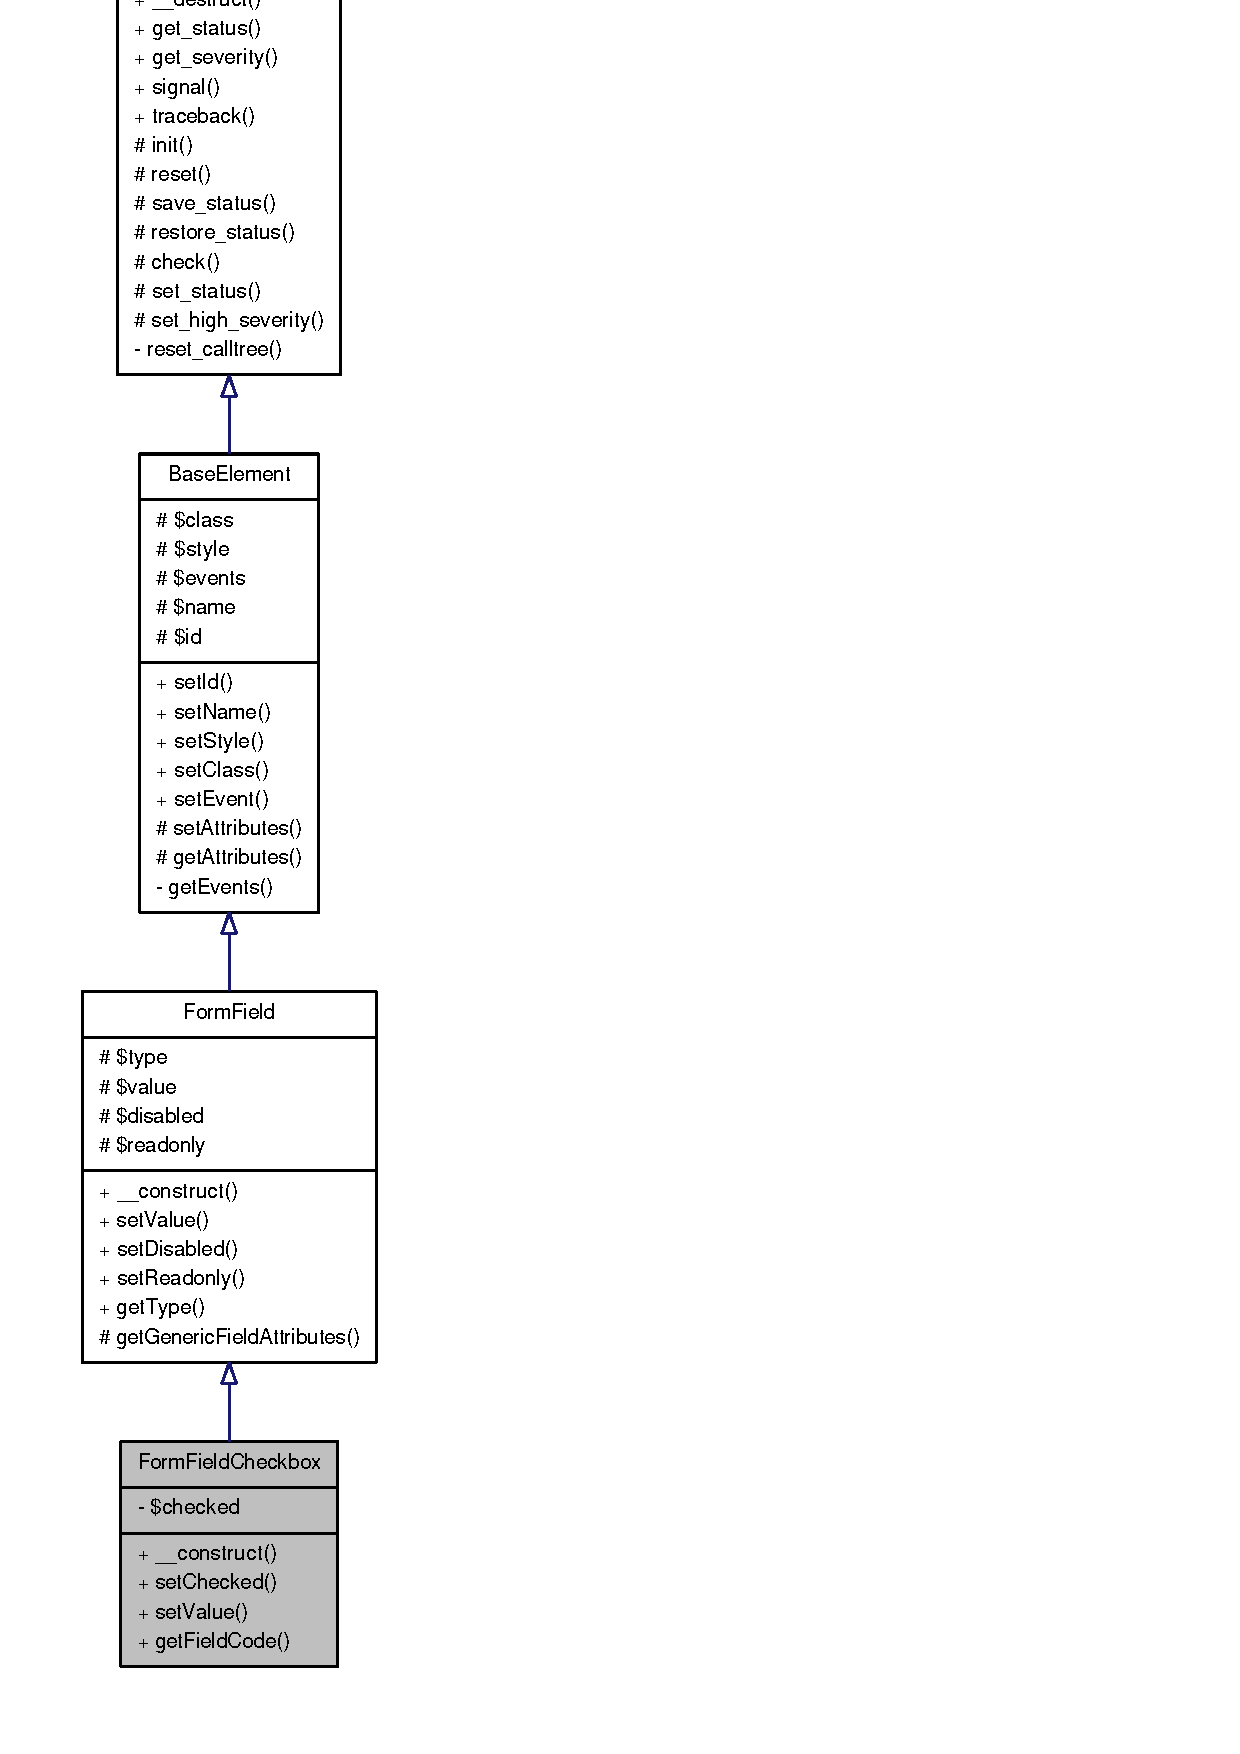
\includegraphics[height=600pt]{classFormFieldCheckbox__coll__graph}
\end{center}
\end{figure}
\subsection*{Public Member Functions}
\begin{DoxyCompactItemize}
\item 
\hyperlink{classFormFieldCheckbox_a9ea37cd03013e361f11680049c1a0097}{\_\-\_\-construct} ()
\item 
\hyperlink{classFormFieldCheckbox_a944623b7e1136bab6dd9880980037425}{setChecked} (\$\_\-value=true)
\item 
\hyperlink{classFormFieldCheckbox_a787abee157599c389a18e0810f69fed5}{setValue} (\$\_\-value)
\item 
\hyperlink{classFormFieldCheckbox_aaa7647c07d938553d8bec7afa869ebc0}{getFieldCode} ()
\item 
\hyperlink{classFormField_a9fa2c828eaf98154edfaa2e755657117}{setDisabled} (\$\_\-value=true)
\item 
\hyperlink{classFormField_a6eabbb35d24b1698ea25b66ddfd88a64}{setReadonly} (\$\_\-value=true)
\item 
\hyperlink{classFormField_a1f64b737bccb6b2827f8c5665b9920c7}{getType} ()
\item 
\hyperlink{classBaseElement_a0c1ce3d1684ecb78960cf7a97278494e}{setId} (\$\_\-value)
\item 
\hyperlink{classBaseElement_a39bafb3609d10048920c20242c2a04c5}{setName} (\$\_\-value)
\item 
\hyperlink{classBaseElement_a6b2b9ff69f6e92db82f91d9c55cda697}{setStyle} (\$\_\-value)
\item 
\hyperlink{classBaseElement_af6597b30fa9798878f6290271043dfa2}{setClass} (\$\_\-value)
\item 
\hyperlink{classBaseElement_ad5789f45f16aaa144716ee8558069c31}{setEvent} (\$\_\-event, \$\_\-action, \$\_\-add=false)
\item 
\hyperlink{class__OWL_a99ec771fa2c5c279f80152cc09e489a8}{get\_\-status} ()
\item 
\hyperlink{class__OWL_adf9509ef96858be7bdd9414c5ef129aa}{get\_\-severity} (\$status=null)
\item 
\hyperlink{class__OWL_a51ba4a16409acf2a2f61f286939091a5}{signal} (\$level=\hyperlink{owl_8severitycodes_8php_a139328861128689f2f4def6a399d9057}{OWL\_\-INFO}, \&\$text=false)
\item 
\hyperlink{class__OWL_aa29547995d6741b7d2b90c1d4ea99a13}{traceback} (\&\$text=false, \$depth=0)
\end{DoxyCompactItemize}
\subsection*{Protected Member Functions}
\begin{DoxyCompactItemize}
\item 
\hyperlink{classFormField_a9f9d136ba8b4a793f22370aff43d592d}{getGenericFieldAttributes} (\$\_\-ignore=array())
\item 
\hyperlink{classBaseElement_aa623b042d23a5b77add8b3c452ec5855}{setAttributes} (\$\_\-attribs)
\item 
\hyperlink{classBaseElement_ae8237038633fc53db818f36da1940297}{getAttributes} (\$\_\-ignore=array())
\item 
\hyperlink{class__OWL_ae0ef3ded56e8a6b34b6461e5a721cd3e}{init} ()
\item 
\hyperlink{class__OWL_a2f2a042bcf31965194c03033df0edc9b}{reset} ()
\item 
\hyperlink{class__OWL_a9e49b9c76fbc021b244c6915ea536d71}{save\_\-status} ()
\item 
\hyperlink{class__OWL_a465eeaf40edd9f9c848841700c32ce55}{restore\_\-status} ()
\item 
\hyperlink{class__OWL_ad6f4f6946f40199dd0333cf219fa500e}{check} (\&\$object, \$level)
\item 
\hyperlink{class__OWL_aea912d0ede9b3c2a69b79072d94d4787}{set\_\-status} (\$status, \$params=array())
\item 
\hyperlink{class__OWL_a576829692a3b66e3d518853bf43abae3}{set\_\-high\_\-severity} (\&\$object=null)
\end{DoxyCompactItemize}
\subsection*{Protected Attributes}
\begin{DoxyCompactItemize}
\item 
\hyperlink{classFormField_a37bed21a1891e95be0e4a697e45ba51b}{\$type}
\item 
\hyperlink{classFormField_a3c01e89834248eec8e2f145fbcfa0fbc}{\$value}
\item 
\hyperlink{classFormField_ab6f1907061890290e32cb2befc0a5f50}{\$disabled}
\item 
\hyperlink{classFormField_a78ba5d4b9127e75e8ccf86f397b5d9ac}{\$readonly}
\item 
\hyperlink{classBaseElement_a99976a8e967db92e7800309f359b0803}{\$class} = ''
\item 
\hyperlink{classBaseElement_a429a3d642dd95f30e1059ef29564b87d}{\$style} = ''
\item 
\hyperlink{classBaseElement_a02cebe45d277b4ff8f29db08bad371ba}{\$events} = array()
\item 
\hyperlink{classBaseElement_a30b8cff187a9de659a70daf287d66f45}{\$name} = ''
\item 
\hyperlink{classBaseElement_a11b6989c43b53869a09f5ce65aa55b45}{\$id} = ''
\item 
\hyperlink{class__OWL_ad26b40a9dbbacb33e299b17826f8327c}{\$severity}
\end{DoxyCompactItemize}
\subsection*{Private Attributes}
\begin{DoxyCompactItemize}
\item 
\hyperlink{classFormFieldCheckbox_a4abeb3a9445b5f31e84e32d257037f2a}{\$checked}
\end{DoxyCompactItemize}


\subsection{Detailed Description}
Formfield. Formfield Checkbox elements \begin{DoxyAuthor}{Author}
Oscar van Eijk, Oveas Functionality Provider 
\end{DoxyAuthor}
\begin{DoxyVersion}{Version}
Oct 19, 2010 -\/-\/ O van Eijk -\/-\/ initial version 
\end{DoxyVersion}


\subsection{Constructor \& Destructor Documentation}
\index{FormFieldCheckbox@{FormFieldCheckbox}!\_\-\_\-construct@{\_\-\_\-construct}}
\index{\_\-\_\-construct@{\_\-\_\-construct}!FormFieldCheckbox@{FormFieldCheckbox}}
\subsubsection[{\_\-\_\-construct}]{\setlength{\rightskip}{0pt plus 5cm}FormFieldCheckbox::\_\-\_\-construct (
\begin{DoxyParamCaption}
{}
\end{DoxyParamCaption}
)}\label{classFormFieldCheckbox_a9ea37cd03013e361f11680049c1a0097}
Class constructor; 

Reimplemented from \hyperlink{classFormField_a0cfe713ce28a6a0cb53476ed463e1f01}{FormField}.



\subsection{Member Function Documentation}
\index{FormFieldCheckbox@{FormFieldCheckbox}!check@{check}}
\index{check@{check}!FormFieldCheckbox@{FormFieldCheckbox}}
\subsubsection[{check}]{\setlength{\rightskip}{0pt plus 5cm}\_\-OWL::check (
\begin{DoxyParamCaption}
\item[{\&\$}]{ object, }
\item[{\$}]{ level}
\end{DoxyParamCaption}
)\hspace{0.3cm}{\ttfamily  \mbox{[}protected, inherited\mbox{]}}}\label{class__OWL_ad6f4f6946f40199dd0333cf219fa500e}
This is a helper function for lazy developers. Some checks have to be made quite often, this is a kinda macro to handle that. It compares the own severity level with that of a given object. If the highest level is above a given max, a traceback and reset are performed.


\begin{DoxyParams}{Parameters}
\item[\mbox{\tt[in]} {\em \$object}]Pointer to an object to check against \item[\mbox{\tt[in]} {\em \$level}]The maximum severity level \end{DoxyParams}
\begin{DoxyReturn}{Returns}
True if the severity level was correct ( below the max), otherwise false 
\end{DoxyReturn}


References \_\-OWL::reset(), \_\-OWL::set\_\-high\_\-severity(), and \_\-OWL::traceback().



Referenced by SessionHandler::write().

\index{FormFieldCheckbox@{FormFieldCheckbox}!get\_\-severity@{get\_\-severity}}
\index{get\_\-severity@{get\_\-severity}!FormFieldCheckbox@{FormFieldCheckbox}}
\subsubsection[{get\_\-severity}]{\setlength{\rightskip}{0pt plus 5cm}\_\-OWL::get\_\-severity (
\begin{DoxyParamCaption}
\item[{\$}]{ status = {\ttfamily null}}
\end{DoxyParamCaption}
)\hspace{0.3cm}{\ttfamily  \mbox{[}inherited\mbox{]}}}\label{class__OWL_adf9509ef96858be7bdd9414c5ef129aa}
Get the current object severity level.


\begin{DoxyParams}{Parameters}
\item[\mbox{\tt[in]} {\em \$status}]An optional parameter to check an other status code i.s.o the object's current status. \end{DoxyParams}
\begin{DoxyReturn}{Returns}
Status severity level 
\end{DoxyReturn}


References \_\-OWL::\$status.



Referenced by LogHandler::compose\_\-message(), LogHandler::log(), and DataHandler::set\_\-key().

\index{FormFieldCheckbox@{FormFieldCheckbox}!get\_\-status@{get\_\-status}}
\index{get\_\-status@{get\_\-status}!FormFieldCheckbox@{FormFieldCheckbox}}
\subsubsection[{get\_\-status}]{\setlength{\rightskip}{0pt plus 5cm}\_\-OWL::get\_\-status (
\begin{DoxyParamCaption}
{}
\end{DoxyParamCaption}
)\hspace{0.3cm}{\ttfamily  \mbox{[}final, inherited\mbox{]}}}\label{class__OWL_a99ec771fa2c5c279f80152cc09e489a8}
Get the current object status.

\begin{DoxyReturn}{Returns}
Object's status code 
\end{DoxyReturn}


Referenced by SchemeHandler::compare().

\index{FormFieldCheckbox@{FormFieldCheckbox}!getAttributes@{getAttributes}}
\index{getAttributes@{getAttributes}!FormFieldCheckbox@{FormFieldCheckbox}}
\subsubsection[{getAttributes}]{\setlength{\rightskip}{0pt plus 5cm}BaseElement::getAttributes (
\begin{DoxyParamCaption}
\item[{\$}]{ \_\-ignore = {\ttfamily array()}}
\end{DoxyParamCaption}
)\hspace{0.3cm}{\ttfamily  \mbox{[}protected, inherited\mbox{]}}}\label{classBaseElement_ae8237038633fc53db818f36da1940297}
Return the general element attributes that are set 
\begin{DoxyParams}{Parameters}
\item[\mbox{\tt[in]} {\em \$\_\-ignore}]Array with attributes names that should be ignored \end{DoxyParams}
\begin{DoxyReturn}{Returns}
string attributes in HTML format (' fld=\char`\"{}value\char`\"{}...) 
\end{DoxyReturn}


References BaseElement::getEvents().



Referenced by FormField::getGenericFieldAttributes(), Table::getTable(), Tablecell::getTablecell(), Tablerow::getTablerow(), and Form::openForm().

\index{FormFieldCheckbox@{FormFieldCheckbox}!getFieldCode@{getFieldCode}}
\index{getFieldCode@{getFieldCode}!FormFieldCheckbox@{FormFieldCheckbox}}
\subsubsection[{getFieldCode}]{\setlength{\rightskip}{0pt plus 5cm}FormFieldCheckbox::getFieldCode (
\begin{DoxyParamCaption}
{}
\end{DoxyParamCaption}
)}\label{classFormFieldCheckbox_aaa7647c07d938553d8bec7afa869ebc0}
Return the HTML code to display the form element

\begin{DoxyReturn}{Returns}
Textstring with the complete code for the form element 
\end{DoxyReturn}


References FormField::getGenericFieldAttributes().

\index{FormFieldCheckbox@{FormFieldCheckbox}!getGenericFieldAttributes@{getGenericFieldAttributes}}
\index{getGenericFieldAttributes@{getGenericFieldAttributes}!FormFieldCheckbox@{FormFieldCheckbox}}
\subsubsection[{getGenericFieldAttributes}]{\setlength{\rightskip}{0pt plus 5cm}FormField::getGenericFieldAttributes (
\begin{DoxyParamCaption}
\item[{\$}]{ \_\-ignore = {\ttfamily array()}}
\end{DoxyParamCaption}
)\hspace{0.3cm}{\ttfamily  \mbox{[}protected, inherited\mbox{]}}}\label{classFormField_a9f9d136ba8b4a793f22370aff43d592d}
Return the attributes for an HTML formfield in the \char`\"{} attrib='value' \mbox{[}...\mbox{]}\char`\"{} format


\begin{DoxyParams}{Parameters}
\item[\mbox{\tt[in]} {\em \$\_\-ignore}]Array with attributes names that should be ignored, e.g. for a textarea, the value is not returned as an attribute. \end{DoxyParams}
\begin{DoxyReturn}{Returns}
Textstring with the HTML code 
\end{DoxyReturn}


References BaseElement::getAttributes().



Referenced by FormFieldTextarea::getFieldCode(), FormFieldText::getFieldCode(), FormFieldSelect::getFieldCode(), FormFieldRadio::getFieldCode(), getFieldCode(), and FormFieldButton::getFieldCode().

\index{FormFieldCheckbox@{FormFieldCheckbox}!getType@{getType}}
\index{getType@{getType}!FormFieldCheckbox@{FormFieldCheckbox}}
\subsubsection[{getType}]{\setlength{\rightskip}{0pt plus 5cm}FormField::getType (
\begin{DoxyParamCaption}
{}
\end{DoxyParamCaption}
)\hspace{0.3cm}{\ttfamily  \mbox{[}inherited\mbox{]}}}\label{classFormField_a1f64b737bccb6b2827f8c5665b9920c7}
Give the field type \begin{DoxyReturn}{Returns}
Field type 
\end{DoxyReturn}
\index{FormFieldCheckbox@{FormFieldCheckbox}!init@{init}}
\index{init@{init}!FormFieldCheckbox@{FormFieldCheckbox}}
\subsubsection[{init}]{\setlength{\rightskip}{0pt plus 5cm}\_\-OWL::init (
\begin{DoxyParamCaption}
{}
\end{DoxyParamCaption}
)\hspace{0.3cm}{\ttfamily  \mbox{[}protected, inherited\mbox{]}}}\label{class__OWL_ae0ef3ded56e8a6b34b6461e5a721cd3e}
This function should be called by all constuctors. It initializes the general characteristics. Status is 'warning' by default, it's up to the contructor to set a proper status; if it's still 'warning', this $\ast$might$\ast$ indicate something went wrong. 

References OWL::factory().



Referenced by Tablerow::\_\-\_\-construct(), Tablecell::\_\-\_\-construct(), Table::\_\-\_\-construct(), FormField::\_\-\_\-construct(), UserHandler::\_\-\_\-construct(), SessionHandler::\_\-\_\-construct(), SchemeHandler::\_\-\_\-construct(), LogHandler::\_\-\_\-construct(), ImageHandler::\_\-\_\-construct(), FormHandler::\_\-\_\-construct(), FileHandler::\_\-\_\-construct(), DbHandler::\_\-\_\-construct(), OWL::\_\-\_\-construct(), Form::\_\-\_\-construct(), Dispatcher::\_\-\_\-construct(), and DataHandler::DataHandler().

\index{FormFieldCheckbox@{FormFieldCheckbox}!reset@{reset}}
\index{reset@{reset}!FormFieldCheckbox@{FormFieldCheckbox}}
\subsubsection[{reset}]{\setlength{\rightskip}{0pt plus 5cm}\_\-OWL::reset (
\begin{DoxyParamCaption}
{}
\end{DoxyParamCaption}
)\hspace{0.3cm}{\ttfamily  \mbox{[}protected, inherited\mbox{]}}}\label{class__OWL_a2f2a042bcf31965194c03033df0edc9b}
General reset function for all objects. Should be called after each non-\/fatal error 

Reimplemented in \hyperlink{classDbHandler_a9982df4830f05803935bb31bac7fae3d}{DbHandler}, and \hyperlink{classSchemeHandler_aa25feb4a70d67b3d571904be4b2f50bc}{SchemeHandler}.



References \_\-OWL::reset\_\-calltree().



Referenced by \_\-OWL::check(), SessionHandler::read(), DataHandler::reset(), and \_\-OWL::set\_\-status().

\index{FormFieldCheckbox@{FormFieldCheckbox}!restore\_\-status@{restore\_\-status}}
\index{restore\_\-status@{restore\_\-status}!FormFieldCheckbox@{FormFieldCheckbox}}
\subsubsection[{restore\_\-status}]{\setlength{\rightskip}{0pt plus 5cm}\_\-OWL::restore\_\-status (
\begin{DoxyParamCaption}
{}
\end{DoxyParamCaption}
)\hspace{0.3cm}{\ttfamily  \mbox{[}protected, inherited\mbox{]}}}\label{class__OWL_a465eeaf40edd9f9c848841700c32ce55}
Restore the previously saved status object and destroy the copy 

References \_\-OWL::set\_\-status().



Referenced by UserHandler::logout().

\index{FormFieldCheckbox@{FormFieldCheckbox}!save\_\-status@{save\_\-status}}
\index{save\_\-status@{save\_\-status}!FormFieldCheckbox@{FormFieldCheckbox}}
\subsubsection[{save\_\-status}]{\setlength{\rightskip}{0pt plus 5cm}\_\-OWL::save\_\-status (
\begin{DoxyParamCaption}
{}
\end{DoxyParamCaption}
)\hspace{0.3cm}{\ttfamily  \mbox{[}protected, inherited\mbox{]}}}\label{class__OWL_a9e49b9c76fbc021b244c6915ea536d71}
Create a copy of the status object 

Referenced by UserHandler::logout().

\index{FormFieldCheckbox@{FormFieldCheckbox}!set\_\-high\_\-severity@{set\_\-high\_\-severity}}
\index{set\_\-high\_\-severity@{set\_\-high\_\-severity}!FormFieldCheckbox@{FormFieldCheckbox}}
\subsubsection[{set\_\-high\_\-severity}]{\setlength{\rightskip}{0pt plus 5cm}\_\-OWL::set\_\-high\_\-severity (
\begin{DoxyParamCaption}
\item[{\&\$}]{ object = {\ttfamily null}}
\end{DoxyParamCaption}
)\hspace{0.3cm}{\ttfamily  \mbox{[}protected, inherited\mbox{]}}}\label{class__OWL_a576829692a3b66e3d518853bf43abae3}
Compare the severity level of the current object with a given one and set my statuspointer to the object with the highest level. 

Referenced by \_\-OWL::check(), DataHandler::db(), DataHandler::prepare(), and SessionHandler::read().

\index{FormFieldCheckbox@{FormFieldCheckbox}!set\_\-status@{set\_\-status}}
\index{set\_\-status@{set\_\-status}!FormFieldCheckbox@{FormFieldCheckbox}}
\subsubsection[{set\_\-status}]{\setlength{\rightskip}{0pt plus 5cm}\_\-OWL::set\_\-status (
\begin{DoxyParamCaption}
\item[{\$}]{ status, }
\item[{\$}]{ params = {\ttfamily array~()}}
\end{DoxyParamCaption}
)\hspace{0.3cm}{\ttfamily  \mbox{[}final, protected, inherited\mbox{]}}}\label{class__OWL_aea912d0ede9b3c2a69b79072d94d4787}
Set the current object status to the specified value.


\begin{DoxyParams}{Parameters}
\item[\mbox{\tt[in]} {\em \$status}]\hyperlink{classOWL}{OWL} status code \item[\mbox{\tt[in]} {\em \$params}]\end{DoxyParams}


References \$GLOBALS, \_\-OWL::\$status, ConfigHandler::get(), Register::get\_\-code(), \_\-OWL::reset(), and \_\-OWL::signal().



Referenced by UserHandler::\_\-\_\-construct(), SessionHandler::\_\-\_\-construct(), SchemeHandler::\_\-\_\-construct(), ImageHandler::\_\-\_\-construct(), FormHandler::\_\-\_\-construct(), FileHandler::\_\-\_\-construct(), DbHandler::\_\-\_\-construct(), Form::\_\-\_\-construct(), Form::addField(), SchemeHandler::alter\_\-scheme(), FileHandler::close(), DbHandler::connect(), DbHandler::create(), SchemeHandler::create\_\-scheme(), DataHandler::DataHandler(), SchemeHandler::define\_\-index(), SchemeHandler::define\_\-scheme(), Dispatcher::dispatch(), FormHandler::get(), DataHandler::get(), SchemeHandler::get\_\-table\_\-columns(), SchemeHandler::get\_\-table\_\-indexes(), UserHandler::login(), FileHandler::open(), DbHandler::open(), LogHandler::open\_\-logfile(), DataHandler::prepare(), DbHandler::prepare\_\-delete(), DbHandler::prepare\_\-insert(), DbHandler::prepare\_\-read(), DbHandler::prepare\_\-update(), DbHandler::read(), FileHandler::read\_\-line(), UserHandler::read\_\-userdata(), \_\-OWL::restore\_\-status(), SchemeHandler::scheme(), FormHandler::set(), DataHandler::set(), DataHandler::set\_\-join(), DataHandler::set\_\-key(), BaseElement::setAttributes(), Form::setEncoding(), Form::setFieldAttributes(), FormFieldText::setMaxsize(), Form::setMethod(), FormFieldRadio::setSelected(), FormFieldText::setSize(), FormFieldSelect::setSize(), FormFieldSelect::setValue(), FormFieldRadio::setValue(), Form::showField(), SchemeHandler::table\_\-description(), SchemeHandler::validate\_\-scheme(), and DbHandler::write().

\index{FormFieldCheckbox@{FormFieldCheckbox}!setAttributes@{setAttributes}}
\index{setAttributes@{setAttributes}!FormFieldCheckbox@{FormFieldCheckbox}}
\subsubsection[{setAttributes}]{\setlength{\rightskip}{0pt plus 5cm}BaseElement::setAttributes (
\begin{DoxyParamCaption}
\item[{\$}]{ \_\-attribs}
\end{DoxyParamCaption}
)\hspace{0.3cm}{\ttfamily  \mbox{[}protected, inherited\mbox{]}}}\label{classBaseElement_aa623b042d23a5b77add8b3c452ec5855}
Set the attributes of the DOM element by calling the 'set$<$Attrib$>$' method for this class. 
\begin{DoxyParams}{Parameters}
\item[\mbox{\tt[in]} {\em \$\_\-attribs}]Array with attributes in the format attrib=$>$value \end{DoxyParams}
\begin{DoxyReturn}{Returns}
Severity level. The status increased when a set$<$Attrib\&gt method does not exist. 
\end{DoxyReturn}


Reimplemented in \hyperlink{classTablecell_a91a8264df222cc44b77ceaf7282a400e}{Tablecell}, and \hyperlink{classTablerow_aece4cad0834c299d7e03030e945aea3a}{Tablerow}.



References \_\-OWL::set\_\-status().



Referenced by Table::\_\-\_\-construct().

\index{FormFieldCheckbox@{FormFieldCheckbox}!setChecked@{setChecked}}
\index{setChecked@{setChecked}!FormFieldCheckbox@{FormFieldCheckbox}}
\subsubsection[{setChecked}]{\setlength{\rightskip}{0pt plus 5cm}FormFieldCheckbox::setChecked (
\begin{DoxyParamCaption}
\item[{\$}]{ \_\-value = {\ttfamily true}}
\end{DoxyParamCaption}
)}\label{classFormFieldCheckbox_a944623b7e1136bab6dd9880980037425}
Set the Checked boolean 
\begin{DoxyParams}{Parameters}
\item[\mbox{\tt[in]} {\em \$\_\-value}]Value indicating true (default) or false \end{DoxyParams}
\index{FormFieldCheckbox@{FormFieldCheckbox}!setClass@{setClass}}
\index{setClass@{setClass}!FormFieldCheckbox@{FormFieldCheckbox}}
\subsubsection[{setClass}]{\setlength{\rightskip}{0pt plus 5cm}BaseElement::setClass (
\begin{DoxyParamCaption}
\item[{\$}]{ \_\-value}
\end{DoxyParamCaption}
)\hspace{0.3cm}{\ttfamily  \mbox{[}inherited\mbox{]}}}\label{classBaseElement_af6597b30fa9798878f6290271043dfa2}
Set the element Class 
\begin{DoxyParams}{Parameters}
\item[\mbox{\tt[in]} {\em \$\_\-value}]Class name \end{DoxyParams}
\index{FormFieldCheckbox@{FormFieldCheckbox}!setDisabled@{setDisabled}}
\index{setDisabled@{setDisabled}!FormFieldCheckbox@{FormFieldCheckbox}}
\subsubsection[{setDisabled}]{\setlength{\rightskip}{0pt plus 5cm}FormField::setDisabled (
\begin{DoxyParamCaption}
\item[{\$}]{ \_\-value = {\ttfamily true}}
\end{DoxyParamCaption}
)\hspace{0.3cm}{\ttfamily  \mbox{[}inherited\mbox{]}}}\label{classFormField_a9fa2c828eaf98154edfaa2e755657117}
Set the Disabled boolean 
\begin{DoxyParams}{Parameters}
\item[\mbox{\tt[in]} {\em \$\_\-value}]Value indicating true (default) or false \end{DoxyParams}
\index{FormFieldCheckbox@{FormFieldCheckbox}!setEvent@{setEvent}}
\index{setEvent@{setEvent}!FormFieldCheckbox@{FormFieldCheckbox}}
\subsubsection[{setEvent}]{\setlength{\rightskip}{0pt plus 5cm}BaseElement::setEvent (
\begin{DoxyParamCaption}
\item[{\$}]{ \_\-event, }
\item[{\$}]{ \_\-action, }
\item[{\$}]{ \_\-add = {\ttfamily false}}
\end{DoxyParamCaption}
)\hspace{0.3cm}{\ttfamily  \mbox{[}inherited\mbox{]}}}\label{classBaseElement_ad5789f45f16aaa144716ee8558069c31}
Add an event to the events array 
\begin{DoxyParams}{Parameters}
\item[\mbox{\tt[in]} {\em \$\_\-event}]Javascript event name (onXxx) \item[\mbox{\tt[in]} {\em \$\_\-action}]Javascript function or code \item[\mbox{\tt[in]} {\em \$\_\-add}]Boolean; when true, the action will be added if the event name already exists. Default is false; overwrite the action for this event. \end{DoxyParams}
\index{FormFieldCheckbox@{FormFieldCheckbox}!setId@{setId}}
\index{setId@{setId}!FormFieldCheckbox@{FormFieldCheckbox}}
\subsubsection[{setId}]{\setlength{\rightskip}{0pt plus 5cm}BaseElement::setId (
\begin{DoxyParamCaption}
\item[{\$}]{ \_\-value}
\end{DoxyParamCaption}
)\hspace{0.3cm}{\ttfamily  \mbox{[}inherited\mbox{]}}}\label{classBaseElement_a0c1ce3d1684ecb78960cf7a97278494e}
Set the element ID 
\begin{DoxyParams}{Parameters}
\item[\mbox{\tt[in]} {\em \$\_\-value}]Identification \end{DoxyParams}
\index{FormFieldCheckbox@{FormFieldCheckbox}!setName@{setName}}
\index{setName@{setName}!FormFieldCheckbox@{FormFieldCheckbox}}
\subsubsection[{setName}]{\setlength{\rightskip}{0pt plus 5cm}BaseElement::setName (
\begin{DoxyParamCaption}
\item[{\$}]{ \_\-value}
\end{DoxyParamCaption}
)\hspace{0.3cm}{\ttfamily  \mbox{[}inherited\mbox{]}}}\label{classBaseElement_a39bafb3609d10048920c20242c2a04c5}
Set the element name 
\begin{DoxyParams}{Parameters}
\item[\mbox{\tt[in]} {\em \$\_\-value}]Element name \end{DoxyParams}
\index{FormFieldCheckbox@{FormFieldCheckbox}!setReadonly@{setReadonly}}
\index{setReadonly@{setReadonly}!FormFieldCheckbox@{FormFieldCheckbox}}
\subsubsection[{setReadonly}]{\setlength{\rightskip}{0pt plus 5cm}FormField::setReadonly (
\begin{DoxyParamCaption}
\item[{\$}]{ \_\-value = {\ttfamily true}}
\end{DoxyParamCaption}
)\hspace{0.3cm}{\ttfamily  \mbox{[}inherited\mbox{]}}}\label{classFormField_a6eabbb35d24b1698ea25b66ddfd88a64}
Set the Readonly boolean 
\begin{DoxyParams}{Parameters}
\item[\mbox{\tt[in]} {\em \$\_\-value}]Value indicating true (default) or false \end{DoxyParams}
\index{FormFieldCheckbox@{FormFieldCheckbox}!setStyle@{setStyle}}
\index{setStyle@{setStyle}!FormFieldCheckbox@{FormFieldCheckbox}}
\subsubsection[{setStyle}]{\setlength{\rightskip}{0pt plus 5cm}BaseElement::setStyle (
\begin{DoxyParamCaption}
\item[{\$}]{ \_\-value}
\end{DoxyParamCaption}
)\hspace{0.3cm}{\ttfamily  \mbox{[}inherited\mbox{]}}}\label{classBaseElement_a6b2b9ff69f6e92db82f91d9c55cda697}
Set the element style 
\begin{DoxyParams}{Parameters}
\item[\mbox{\tt[in]} {\em \$\_\-value}]Element style \end{DoxyParams}
\index{FormFieldCheckbox@{FormFieldCheckbox}!setValue@{setValue}}
\index{setValue@{setValue}!FormFieldCheckbox@{FormFieldCheckbox}}
\subsubsection[{setValue}]{\setlength{\rightskip}{0pt plus 5cm}FormFieldCheckbox::setValue (
\begin{DoxyParamCaption}
\item[{\$}]{ \_\-value}
\end{DoxyParamCaption}
)}\label{classFormFieldCheckbox_a787abee157599c389a18e0810f69fed5}
Reimplement; value defaults to 1 for checkboxes 
\begin{DoxyParams}{Parameters}
\item[\mbox{\tt[in]} {\em \$\_\-value}]Field value \end{DoxyParams}


Reimplemented from \hyperlink{classFormField_a465ff61e290d82be96bb793c3a14b3e7}{FormField}.

\index{FormFieldCheckbox@{FormFieldCheckbox}!signal@{signal}}
\index{signal@{signal}!FormFieldCheckbox@{FormFieldCheckbox}}
\subsubsection[{signal}]{\setlength{\rightskip}{0pt plus 5cm}\_\-OWL::signal (
\begin{DoxyParamCaption}
\item[{\$}]{ level = {\ttfamily {\bf OWL\_\-INFO}}, }
\item[{\&\$}]{ text = {\ttfamily false}}
\end{DoxyParamCaption}
)\hspace{0.3cm}{\ttfamily  \mbox{[}inherited\mbox{]}}}\label{class__OWL_a51ba4a16409acf2a2f61f286939091a5}
Display the message for the current object status


\begin{DoxyParams}{Parameters}
\item[\mbox{\tt[in]} {\em \$level}]An optional severity level; message will only be displayed when it is at least of this level. \item[\mbox{\tt[out]} {\em \$text}]If this parameter is given, the message text is returned in this string instead of echood. \end{DoxyParams}
\begin{DoxyReturn}{Returns}
The severity level for this object 
\end{DoxyReturn}


References ConfigHandler::get().



Referenced by \_\-OWL::set\_\-status(), and \_\-OWL::traceback().

\index{FormFieldCheckbox@{FormFieldCheckbox}!traceback@{traceback}}
\index{traceback@{traceback}!FormFieldCheckbox@{FormFieldCheckbox}}
\subsubsection[{traceback}]{\setlength{\rightskip}{0pt plus 5cm}\_\-OWL::traceback (
\begin{DoxyParamCaption}
\item[{\&\$}]{ text = {\ttfamily false}, }
\item[{\$}]{ depth = {\ttfamily 0}}
\end{DoxyParamCaption}
)\hspace{0.3cm}{\ttfamily  \mbox{[}inherited\mbox{]}}}\label{class__OWL_aa29547995d6741b7d2b90c1d4ea99a13}
If somehwere in the nested calls an error occured, we can traceback the original failing object with this function and signal the message.


\begin{DoxyParams}{Parameters}
\item[\mbox{\tt[out]} {\em \$text}]Optional variable in which the message text can be stored. If not given, the text will be written to standard output \item[\mbox{\tt[in]} {\em \$depth}]This paramater should be initially empty. It calculates the depth in recursive calls. \end{DoxyParams}
\begin{DoxyReturn}{Returns}
Severity code of the failing object 
\end{DoxyReturn}


References \_\-OWL::signal().



Referenced by \_\-OWL::check(), UserHandler::login(), and SessionHandler::read().



\subsection{Member Data Documentation}
\index{FormFieldCheckbox@{FormFieldCheckbox}!\$checked@{\$checked}}
\index{\$checked@{\$checked}!FormFieldCheckbox@{FormFieldCheckbox}}
\subsubsection[{\$checked}]{\setlength{\rightskip}{0pt plus 5cm}FormFieldCheckbox::\$checked\hspace{0.3cm}{\ttfamily  \mbox{[}private\mbox{]}}}\label{classFormFieldCheckbox_a4abeb3a9445b5f31e84e32d257037f2a}
Boolean set to true when the box is checked \index{FormFieldCheckbox@{FormFieldCheckbox}!\$class@{\$class}}
\index{\$class@{\$class}!FormFieldCheckbox@{FormFieldCheckbox}}
\subsubsection[{\$class}]{\setlength{\rightskip}{0pt plus 5cm}BaseElement::\$class = ''\hspace{0.3cm}{\ttfamily  \mbox{[}protected, inherited\mbox{]}}}\label{classBaseElement_a99976a8e967db92e7800309f359b0803}
Class specification \index{FormFieldCheckbox@{FormFieldCheckbox}!\$disabled@{\$disabled}}
\index{\$disabled@{\$disabled}!FormFieldCheckbox@{FormFieldCheckbox}}
\subsubsection[{\$disabled}]{\setlength{\rightskip}{0pt plus 5cm}FormField::\$disabled\hspace{0.3cm}{\ttfamily  \mbox{[}protected, inherited\mbox{]}}}\label{classFormField_ab6f1907061890290e32cb2befc0a5f50}
Boolean indicating a disabled field when true \index{FormFieldCheckbox@{FormFieldCheckbox}!\$events@{\$events}}
\index{\$events@{\$events}!FormFieldCheckbox@{FormFieldCheckbox}}
\subsubsection[{\$events}]{\setlength{\rightskip}{0pt plus 5cm}BaseElement::\$events = array()\hspace{0.3cm}{\ttfamily  \mbox{[}protected, inherited\mbox{]}}}\label{classBaseElement_a02cebe45d277b4ff8f29db08bad371ba}
Array with javascript events 

Referenced by Form::setFieldEvents().

\index{FormFieldCheckbox@{FormFieldCheckbox}!\$id@{\$id}}
\index{\$id@{\$id}!FormFieldCheckbox@{FormFieldCheckbox}}
\subsubsection[{\$id}]{\setlength{\rightskip}{0pt plus 5cm}BaseElement::\$id = ''\hspace{0.3cm}{\ttfamily  \mbox{[}protected, inherited\mbox{]}}}\label{classBaseElement_a11b6989c43b53869a09f5ce65aa55b45}
Element ID \index{FormFieldCheckbox@{FormFieldCheckbox}!\$name@{\$name}}
\index{\$name@{\$name}!FormFieldCheckbox@{FormFieldCheckbox}}
\subsubsection[{\$name}]{\setlength{\rightskip}{0pt plus 5cm}BaseElement::\$name = ''\hspace{0.3cm}{\ttfamily  \mbox{[}protected, inherited\mbox{]}}}\label{classBaseElement_a30b8cff187a9de659a70daf287d66f45}
Name of the element 

Referenced by Form::addField(), and Form::showField().

\index{FormFieldCheckbox@{FormFieldCheckbox}!\$readonly@{\$readonly}}
\index{\$readonly@{\$readonly}!FormFieldCheckbox@{FormFieldCheckbox}}
\subsubsection[{\$readonly}]{\setlength{\rightskip}{0pt plus 5cm}FormField::\$readonly\hspace{0.3cm}{\ttfamily  \mbox{[}protected, inherited\mbox{]}}}\label{classFormField_a78ba5d4b9127e75e8ccf86f397b5d9ac}
Boolean indicating a readonly field when true \index{FormFieldCheckbox@{FormFieldCheckbox}!\$severity@{\$severity}}
\index{\$severity@{\$severity}!FormFieldCheckbox@{FormFieldCheckbox}}
\subsubsection[{\$severity}]{\setlength{\rightskip}{0pt plus 5cm}\_\-OWL::\$severity\hspace{0.3cm}{\ttfamily  \mbox{[}protected, inherited\mbox{]}}}\label{class__OWL_ad26b40a9dbbacb33e299b17826f8327c}
Severity level of the current object status \index{FormFieldCheckbox@{FormFieldCheckbox}!\$style@{\$style}}
\index{\$style@{\$style}!FormFieldCheckbox@{FormFieldCheckbox}}
\subsubsection[{\$style}]{\setlength{\rightskip}{0pt plus 5cm}BaseElement::\$style = ''\hspace{0.3cm}{\ttfamily  \mbox{[}protected, inherited\mbox{]}}}\label{classBaseElement_a429a3d642dd95f30e1059ef29564b87d}
Element style \index{FormFieldCheckbox@{FormFieldCheckbox}!\$type@{\$type}}
\index{\$type@{\$type}!FormFieldCheckbox@{FormFieldCheckbox}}
\subsubsection[{\$type}]{\setlength{\rightskip}{0pt plus 5cm}FormField::\$type\hspace{0.3cm}{\ttfamily  \mbox{[}protected, inherited\mbox{]}}}\label{classFormField_a37bed21a1891e95be0e4a697e45ba51b}
Field type 

Reimplemented in \hyperlink{classFormFieldTextarea_a85348034822c70694fc8640bfcacc04d}{FormFieldTextarea}.



Referenced by FormFieldText::\_\-\_\-construct(), and FormFieldButton::\_\-\_\-construct().

\index{FormFieldCheckbox@{FormFieldCheckbox}!\$value@{\$value}}
\index{\$value@{\$value}!FormFieldCheckbox@{FormFieldCheckbox}}
\subsubsection[{\$value}]{\setlength{\rightskip}{0pt plus 5cm}FormField::\$value\hspace{0.3cm}{\ttfamily  \mbox{[}protected, inherited\mbox{]}}}\label{classFormField_a3c01e89834248eec8e2f145fbcfa0fbc}
Field value 

The documentation for this class was generated from the following file:\begin{DoxyCompactItemize}
\item 
/home/oscar/projects/owl-\/php/src/kernel/ui/formfields/\hyperlink{class_8formfield_8checkbox_8php}{class.formfield.checkbox.php}\end{DoxyCompactItemize}

\section{FormFieldFile Class Reference}
\label{classFormFieldFile}\index{FormFieldFile@{FormFieldFile}}


Formfield.  




Inheritance diagram for FormFieldFile:\nopagebreak
\begin{figure}[H]
\begin{center}
\leavevmode
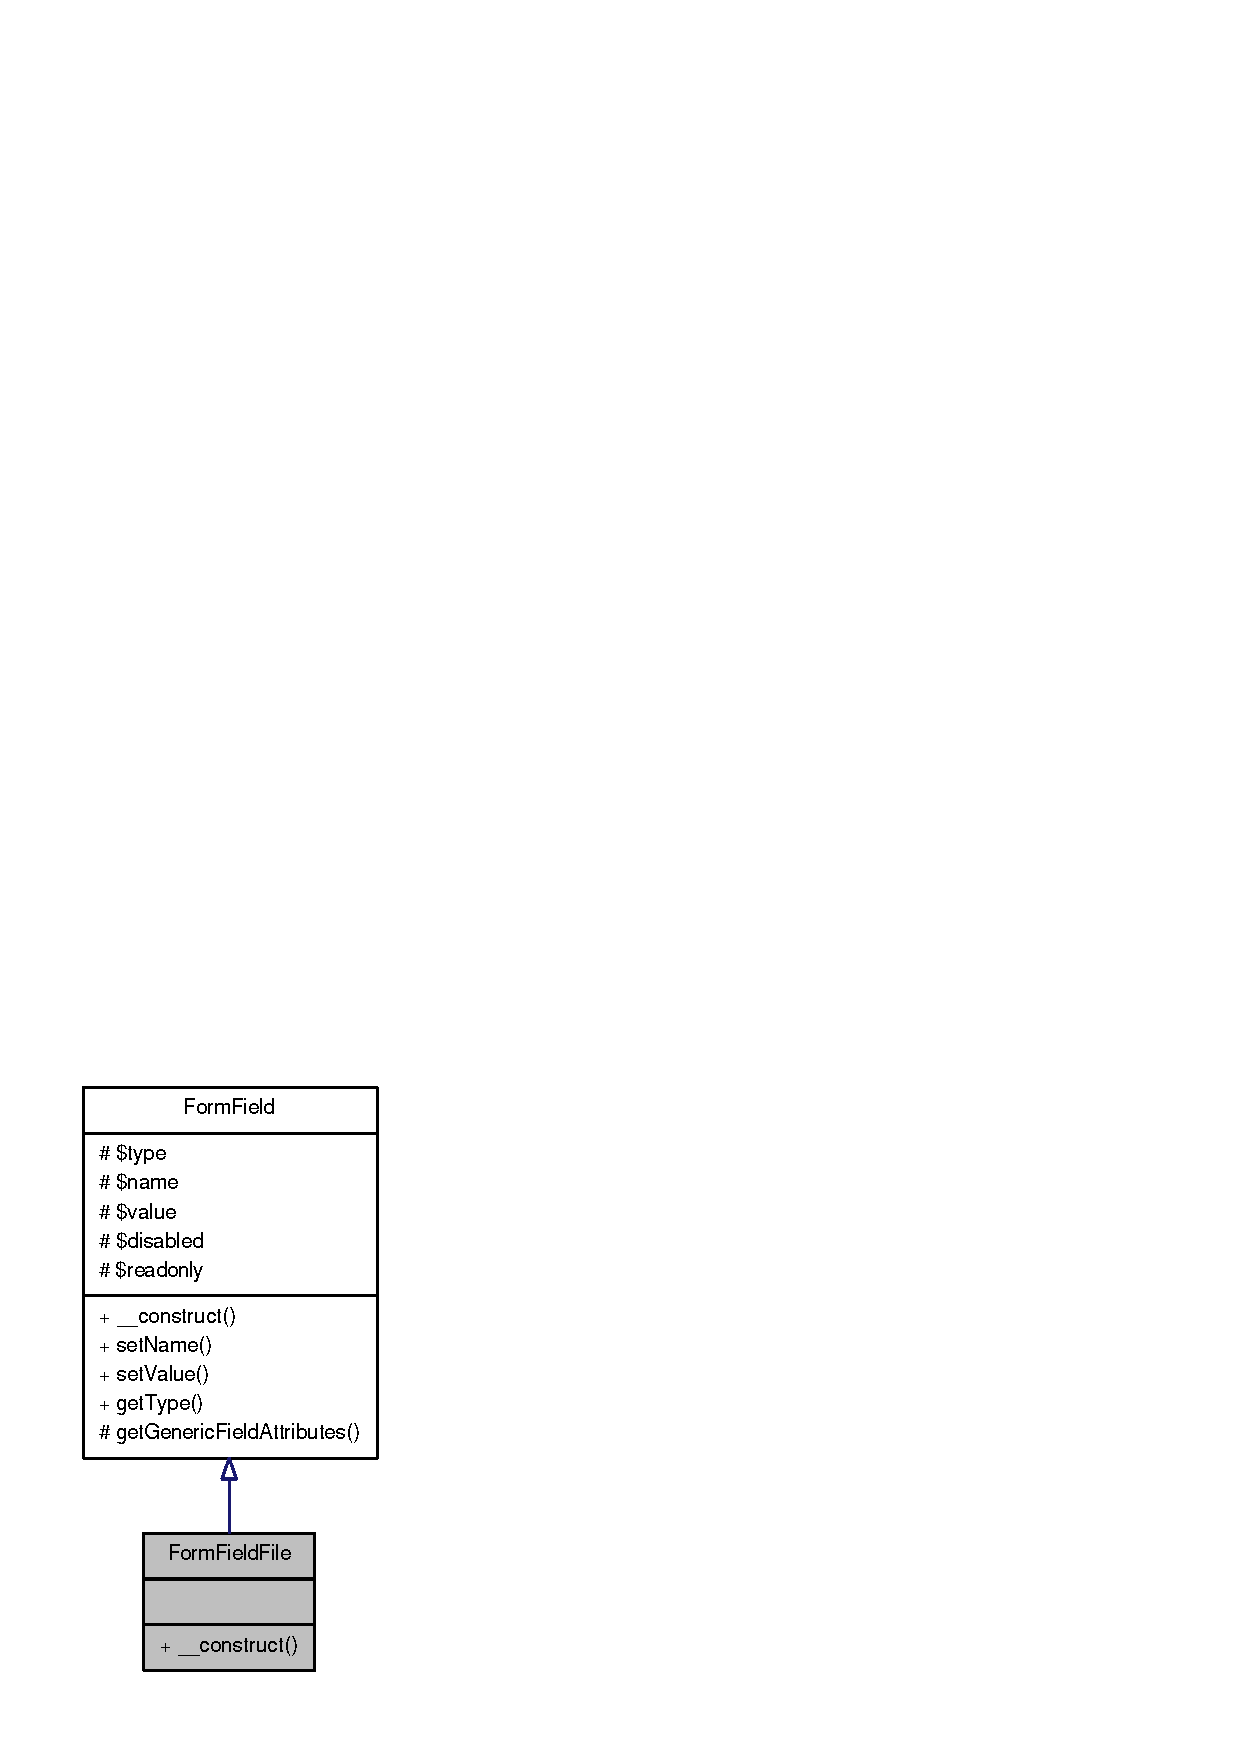
\includegraphics[height=400pt]{classFormFieldFile__inherit__graph}
\end{center}
\end{figure}


Collaboration diagram for FormFieldFile:\nopagebreak
\begin{figure}[H]
\begin{center}
\leavevmode
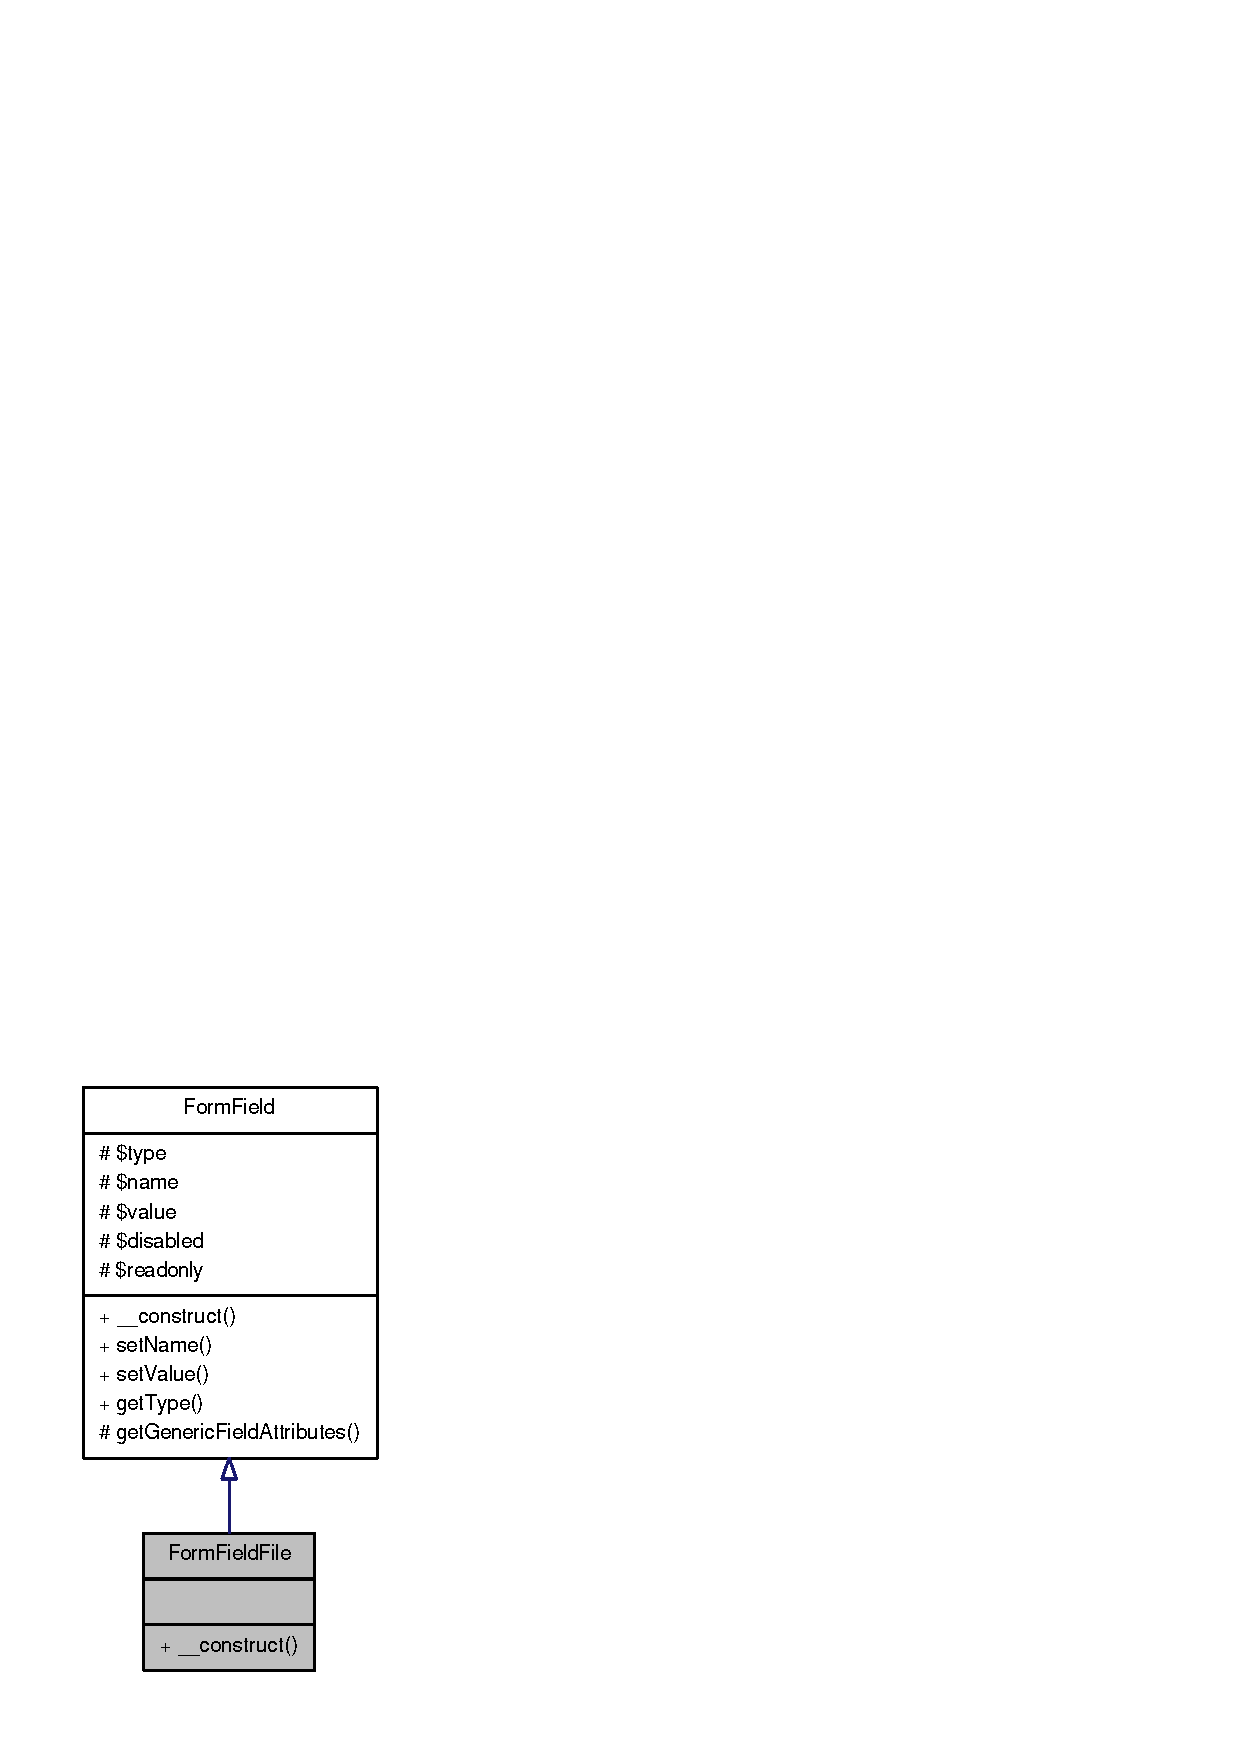
\includegraphics[height=400pt]{classFormFieldFile__coll__graph}
\end{center}
\end{figure}
\subsection*{Public Member Functions}
\begin{DoxyCompactItemize}
\item 
\hyperlink{classFormFieldFile_a2e19b30454dd3ed054772868bf6eebad}{\_\-\_\-construct} ()
\item 
\hyperlink{classFormField_ad57e32bd53170af060e869b3b60f0ef7}{setName} (\$\_\-value)
\item 
\hyperlink{classFormField_a465ff61e290d82be96bb793c3a14b3e7}{setValue} (\$\_\-value)
\item 
\hyperlink{classFormField_a9fa2c828eaf98154edfaa2e755657117}{setDisabled} (\$\_\-value=true)
\item 
\hyperlink{classFormField_a6eabbb35d24b1698ea25b66ddfd88a64}{setReadonly} (\$\_\-value=true)
\item 
\hyperlink{classFormField_a1f64b737bccb6b2827f8c5665b9920c7}{getType} ()
\item 
\hyperlink{classBaseElement_a0c1ce3d1684ecb78960cf7a97278494e}{setId} (\$\_\-value)
\item 
\hyperlink{classBaseElement_af6597b30fa9798878f6290271043dfa2}{setClass} (\$\_\-value)
\item 
\hyperlink{class__OWL_a99ec771fa2c5c279f80152cc09e489a8}{get\_\-status} ()
\item 
\hyperlink{class__OWL_adf9509ef96858be7bdd9414c5ef129aa}{get\_\-severity} (\$status=null)
\item 
\hyperlink{class__OWL_a51ba4a16409acf2a2f61f286939091a5}{signal} (\$level=\hyperlink{owl_8severitycodes_8php_a139328861128689f2f4def6a399d9057}{OWL\_\-INFO}, \&\$text=false)
\item 
\hyperlink{class__OWL_aa29547995d6741b7d2b90c1d4ea99a13}{traceback} (\&\$text=false, \$depth=0)
\end{DoxyCompactItemize}
\subsection*{Protected Member Functions}
\begin{DoxyCompactItemize}
\item 
\hyperlink{classFormField_a9f9d136ba8b4a793f22370aff43d592d}{getGenericFieldAttributes} (\$\_\-ignore=array())
\item 
\hyperlink{classBaseElement_a852277a83d867417f2e39e8a2483bac7}{getEvents} ()
\item 
\hyperlink{classBaseElement_a25bed980efe965e95dc43d7c2fa1faca}{getAttributes} ()
\item 
\hyperlink{class__OWL_ae0ef3ded56e8a6b34b6461e5a721cd3e}{init} ()
\item 
\hyperlink{class__OWL_a2f2a042bcf31965194c03033df0edc9b}{reset} ()
\item 
\hyperlink{class__OWL_ad6f4f6946f40199dd0333cf219fa500e}{check} (\&\$object, \$level)
\item 
\hyperlink{class__OWL_aea912d0ede9b3c2a69b79072d94d4787}{set\_\-status} (\$status, \$params=array())
\item 
\hyperlink{class__OWL_a576829692a3b66e3d518853bf43abae3}{set\_\-high\_\-severity} (\&\$object=null)
\end{DoxyCompactItemize}
\subsection*{Protected Attributes}
\begin{DoxyCompactItemize}
\item 
\hyperlink{classFormField_a37bed21a1891e95be0e4a697e45ba51b}{\$type}
\item 
\hyperlink{classFormField_a23861f707bcd77bbace6300de9621746}{\$name}
\item 
\hyperlink{classFormField_a3c01e89834248eec8e2f145fbcfa0fbc}{\$value}
\item 
\hyperlink{classFormField_ab6f1907061890290e32cb2befc0a5f50}{\$disabled}
\item 
\hyperlink{classFormField_a78ba5d4b9127e75e8ccf86f397b5d9ac}{\$readonly}
\item 
\hyperlink{classBaseElement_a99976a8e967db92e7800309f359b0803}{\$class} = ''
\item 
\hyperlink{classBaseElement_a429a3d642dd95f30e1059ef29564b87d}{\$style} = ''
\item 
\hyperlink{classBaseElement_a11b6989c43b53869a09f5ce65aa55b45}{\$id} = ''
\item 
\hyperlink{class__OWL_ad26b40a9dbbacb33e299b17826f8327c}{\$severity}
\end{DoxyCompactItemize}


\subsection{Detailed Description}
Formfield. Formfield File input elements \begin{DoxyAuthor}{Author}
Oscar van Eijk, Oveas Functionality Provider 
\end{DoxyAuthor}
\begin{DoxyVersion}{Version}
Oct 19, 2010 -\/-\/ O van Eijk -\/-\/ initial version 
\end{DoxyVersion}


\subsection{Constructor \& Destructor Documentation}
\index{FormFieldFile@{FormFieldFile}!\_\-\_\-construct@{\_\-\_\-construct}}
\index{\_\-\_\-construct@{\_\-\_\-construct}!FormFieldFile@{FormFieldFile}}
\subsubsection[{\_\-\_\-construct}]{\setlength{\rightskip}{0pt plus 5cm}FormFieldFile::\_\-\_\-construct ()}\label{classFormFieldFile_a2e19b30454dd3ed054772868bf6eebad}
Class constructor; 

Reimplemented from \hyperlink{classFormField_a0cfe713ce28a6a0cb53476ed463e1f01}{FormField}.



\subsection{Member Function Documentation}
\index{FormFieldFile@{FormFieldFile}!check@{check}}
\index{check@{check}!FormFieldFile@{FormFieldFile}}
\subsubsection[{check}]{\setlength{\rightskip}{0pt plus 5cm}\_\-OWL::check (\&\$ {\em object}, \/  \$ {\em level})\hspace{0.3cm}{\ttfamily  \mbox{[}protected, inherited\mbox{]}}}\label{class__OWL_ad6f4f6946f40199dd0333cf219fa500e}
This is a helper function for lazy developers. Some checks have to be made quite often, this is a kinda macro to handle that. It compares the own severity level with that of a given object. If the highest level is above a given max, a traceback and reset are performed.


\begin{DoxyParams}{Parameters}
\item[\mbox{$\leftarrow$} {\em \$object}]Pointer to an object to check against \item[\mbox{$\leftarrow$} {\em \$level}]The maximum severity level \end{DoxyParams}
\begin{DoxyReturn}{Returns}
True if the severity level was correct ( below the max), otherwise false 
\end{DoxyReturn}


References \_\-OWL::reset(), \_\-OWL::set\_\-high\_\-severity(), and \_\-OWL::traceback().



Referenced by SessionHandler::write().

\index{FormFieldFile@{FormFieldFile}!get\_\-severity@{get\_\-severity}}
\index{get\_\-severity@{get\_\-severity}!FormFieldFile@{FormFieldFile}}
\subsubsection[{get\_\-severity}]{\setlength{\rightskip}{0pt plus 5cm}\_\-OWL::get\_\-severity (\$ {\em status} = {\ttfamily null})\hspace{0.3cm}{\ttfamily  \mbox{[}inherited\mbox{]}}}\label{class__OWL_adf9509ef96858be7bdd9414c5ef129aa}
Get the current object severity level.


\begin{DoxyParams}{Parameters}
\item[\mbox{$\leftarrow$} {\em \$status}]An optional parameter to check an other status code i.s.o the object's current status. \end{DoxyParams}
\begin{DoxyReturn}{Returns}
Status severity level 
\end{DoxyReturn}


References \_\-OWL::\$status.



Referenced by LogHandler::compose\_\-message(), LogHandler::log(), and DataHandler::set\_\-key().

\index{FormFieldFile@{FormFieldFile}!get\_\-status@{get\_\-status}}
\index{get\_\-status@{get\_\-status}!FormFieldFile@{FormFieldFile}}
\subsubsection[{get\_\-status}]{\setlength{\rightskip}{0pt plus 5cm}\_\-OWL::get\_\-status ()\hspace{0.3cm}{\ttfamily  \mbox{[}final, inherited\mbox{]}}}\label{class__OWL_a99ec771fa2c5c279f80152cc09e489a8}
Get the current object status.

\begin{DoxyReturn}{Returns}
Object's status code 
\end{DoxyReturn}


Referenced by SchemeHandler::compare().

\index{FormFieldFile@{FormFieldFile}!getAttributes@{getAttributes}}
\index{getAttributes@{getAttributes}!FormFieldFile@{FormFieldFile}}
\subsubsection[{getAttributes}]{\setlength{\rightskip}{0pt plus 5cm}BaseElement::getAttributes ()\hspace{0.3cm}{\ttfamily  \mbox{[}protected, inherited\mbox{]}}}\label{classBaseElement_a25bed980efe965e95dc43d7c2fa1faca}
Return the general element attributes that are set \begin{DoxyReturn}{Returns}
string attributes in HTML format (' fld=\char`\"{}value\char`\"{}...) 
\end{DoxyReturn}


Referenced by Form::openForm().

\index{FormFieldFile@{FormFieldFile}!getEvents@{getEvents}}
\index{getEvents@{getEvents}!FormFieldFile@{FormFieldFile}}
\subsubsection[{getEvents}]{\setlength{\rightskip}{0pt plus 5cm}BaseElement::getEvents ()\hspace{0.3cm}{\ttfamily  \mbox{[}protected, inherited\mbox{]}}}\label{classBaseElement_a852277a83d867417f2e39e8a2483bac7}


Referenced by FormField::getGenericFieldAttributes().

\index{FormFieldFile@{FormFieldFile}!getGenericFieldAttributes@{getGenericFieldAttributes}}
\index{getGenericFieldAttributes@{getGenericFieldAttributes}!FormFieldFile@{FormFieldFile}}
\subsubsection[{getGenericFieldAttributes}]{\setlength{\rightskip}{0pt plus 5cm}FormField::getGenericFieldAttributes (\$ {\em \_\-ignore} = {\ttfamily array()})\hspace{0.3cm}{\ttfamily  \mbox{[}protected, inherited\mbox{]}}}\label{classFormField_a9f9d136ba8b4a793f22370aff43d592d}
Return the attributes for an HTML formfield in the \char`\"{} attrib='value' \mbox{[}...\mbox{]}\char`\"{} format


\begin{DoxyParams}{Parameters}
\item[\mbox{$\leftarrow$} {\em \$\_\-ignore}]Array with attributes names that should be ignored, e.g. for a textarea, the value is not returned as an attribute. \end{DoxyParams}
\begin{DoxyReturn}{Returns}
Textstring with the HTML code 
\end{DoxyReturn}


References BaseElement::getEvents().



Referenced by FormFieldTextarea::getFieldCode(), FormFieldText::getFieldCode(), FormFieldSelect::getFieldCode(), FormFieldRadio::getFieldCode(), FormFieldCheckbox::getFieldCode(), and FormFieldButton::getFieldCode().

\index{FormFieldFile@{FormFieldFile}!getType@{getType}}
\index{getType@{getType}!FormFieldFile@{FormFieldFile}}
\subsubsection[{getType}]{\setlength{\rightskip}{0pt plus 5cm}FormField::getType ()\hspace{0.3cm}{\ttfamily  \mbox{[}inherited\mbox{]}}}\label{classFormField_a1f64b737bccb6b2827f8c5665b9920c7}
Give the field type \begin{DoxyReturn}{Returns}
Field type 
\end{DoxyReturn}
\index{FormFieldFile@{FormFieldFile}!init@{init}}
\index{init@{init}!FormFieldFile@{FormFieldFile}}
\subsubsection[{init}]{\setlength{\rightskip}{0pt plus 5cm}\_\-OWL::init ()\hspace{0.3cm}{\ttfamily  \mbox{[}protected, inherited\mbox{]}}}\label{class__OWL_ae0ef3ded56e8a6b34b6461e5a721cd3e}
This function should be called by all constuctors. It initializes the general characteristics. Status is 'warning' by default, it's up to the contructor to set a proper status; if it's still 'warning', this $\ast$might$\ast$ indicate something went wrong. 

References OWL::factory().



Referenced by UserHandler::\_\-\_\-construct(), SessionHandler::\_\-\_\-construct(), SchemeHandler::\_\-\_\-construct(), LogHandler::\_\-\_\-construct(), ImageHandler::\_\-\_\-construct(), FormHandler::\_\-\_\-construct(), FileHandler::\_\-\_\-construct(), DbHandler::\_\-\_\-construct(), OWL::\_\-\_\-construct(), Dispatcher::\_\-\_\-construct(), and DataHandler::DataHandler().

\index{FormFieldFile@{FormFieldFile}!reset@{reset}}
\index{reset@{reset}!FormFieldFile@{FormFieldFile}}
\subsubsection[{reset}]{\setlength{\rightskip}{0pt plus 5cm}\_\-OWL::reset ()\hspace{0.3cm}{\ttfamily  \mbox{[}protected, inherited\mbox{]}}}\label{class__OWL_a2f2a042bcf31965194c03033df0edc9b}
General reset function for all objects. Should be called after each non-\/fatal error 

Reimplemented in \hyperlink{classDbHandler_a9982df4830f05803935bb31bac7fae3d}{DbHandler}, and \hyperlink{classSchemeHandler_aa25feb4a70d67b3d571904be4b2f50bc}{SchemeHandler}.



References \_\-OWL::reset\_\-calltree().



Referenced by \_\-OWL::check(), SessionHandler::read(), DataHandler::reset(), and \_\-OWL::set\_\-status().

\index{FormFieldFile@{FormFieldFile}!set\_\-high\_\-severity@{set\_\-high\_\-severity}}
\index{set\_\-high\_\-severity@{set\_\-high\_\-severity}!FormFieldFile@{FormFieldFile}}
\subsubsection[{set\_\-high\_\-severity}]{\setlength{\rightskip}{0pt plus 5cm}\_\-OWL::set\_\-high\_\-severity (\&\$ {\em object} = {\ttfamily null})\hspace{0.3cm}{\ttfamily  \mbox{[}protected, inherited\mbox{]}}}\label{class__OWL_a576829692a3b66e3d518853bf43abae3}
Compare the severity level of the current object with a given one and set my statuspointer to the object with the highest level. 

Referenced by \_\-OWL::check(), DataHandler::db(), DataHandler::prepare(), and SessionHandler::read().

\index{FormFieldFile@{FormFieldFile}!set\_\-status@{set\_\-status}}
\index{set\_\-status@{set\_\-status}!FormFieldFile@{FormFieldFile}}
\subsubsection[{set\_\-status}]{\setlength{\rightskip}{0pt plus 5cm}\_\-OWL::set\_\-status (\$ {\em status}, \/  \$ {\em params} = {\ttfamily array~()})\hspace{0.3cm}{\ttfamily  \mbox{[}final, protected, inherited\mbox{]}}}\label{class__OWL_aea912d0ede9b3c2a69b79072d94d4787}
Set the current object status to the specified value.


\begin{DoxyParams}{Parameters}
\item[\mbox{$\leftarrow$} {\em \$status}]\hyperlink{classOWL}{OWL} status code \item[\mbox{$\leftarrow$} {\em \$params}]\end{DoxyParams}


References \$GLOBALS, \_\-OWL::\$status, ConfigHandler::get(), Register::get\_\-code(), \_\-OWL::reset(), and \_\-OWL::signal().



Referenced by UserHandler::\_\-\_\-construct(), SessionHandler::\_\-\_\-construct(), SchemeHandler::\_\-\_\-construct(), ImageHandler::\_\-\_\-construct(), FormHandler::\_\-\_\-construct(), FileHandler::\_\-\_\-construct(), DbHandler::\_\-\_\-construct(), Form::addField(), SchemeHandler::alter\_\-scheme(), FileHandler::close(), DbHandler::connect(), DbHandler::create(), SchemeHandler::create\_\-scheme(), DataHandler::DataHandler(), SchemeHandler::define\_\-index(), SchemeHandler::define\_\-scheme(), Dispatcher::dispatch(), FormHandler::get(), DataHandler::get(), SchemeHandler::get\_\-table\_\-columns(), SchemeHandler::get\_\-table\_\-indexes(), UserHandler::login(), FileHandler::open(), DbHandler::open(), LogHandler::open\_\-logfile(), DataHandler::prepare(), DbHandler::prepare\_\-delete(), DbHandler::prepare\_\-insert(), DbHandler::prepare\_\-read(), DbHandler::prepare\_\-update(), DbHandler::read(), FileHandler::read\_\-line(), UserHandler::read\_\-userdata(), DataHandler::reset(), SchemeHandler::scheme(), FormHandler::set(), DataHandler::set(), DataHandler::set\_\-join(), DataHandler::set\_\-key(), Form::setFieldAttributes(), FormFieldText::setMaxsize(), FormFieldRadio::setSelected(), FormFieldText::setSize(), FormFieldSelect::setSize(), FormFieldSelect::setValue(), FormFieldRadio::setValue(), Form::showField(), SchemeHandler::table\_\-description(), SchemeHandler::validate\_\-scheme(), and DbHandler::write().

\index{FormFieldFile@{FormFieldFile}!setClass@{setClass}}
\index{setClass@{setClass}!FormFieldFile@{FormFieldFile}}
\subsubsection[{setClass}]{\setlength{\rightskip}{0pt plus 5cm}BaseElement::setClass (\$ {\em \_\-value})\hspace{0.3cm}{\ttfamily  \mbox{[}inherited\mbox{]}}}\label{classBaseElement_af6597b30fa9798878f6290271043dfa2}
Set the element Class 
\begin{DoxyParams}{Parameters}
\item[\mbox{$\leftarrow$} {\em \$\_\-value}]Class name \end{DoxyParams}
\index{FormFieldFile@{FormFieldFile}!setDisabled@{setDisabled}}
\index{setDisabled@{setDisabled}!FormFieldFile@{FormFieldFile}}
\subsubsection[{setDisabled}]{\setlength{\rightskip}{0pt plus 5cm}FormField::setDisabled (\$ {\em \_\-value} = {\ttfamily true})\hspace{0.3cm}{\ttfamily  \mbox{[}inherited\mbox{]}}}\label{classFormField_a9fa2c828eaf98154edfaa2e755657117}
Set the Disabled boolean 
\begin{DoxyParams}{Parameters}
\item[\mbox{$\leftarrow$} {\em \$\_\-value}]Value indicating true (default) or false \end{DoxyParams}
\index{FormFieldFile@{FormFieldFile}!setId@{setId}}
\index{setId@{setId}!FormFieldFile@{FormFieldFile}}
\subsubsection[{setId}]{\setlength{\rightskip}{0pt plus 5cm}BaseElement::setId (\$ {\em \_\-value})\hspace{0.3cm}{\ttfamily  \mbox{[}inherited\mbox{]}}}\label{classBaseElement_a0c1ce3d1684ecb78960cf7a97278494e}
Set the element ID 
\begin{DoxyParams}{Parameters}
\item[\mbox{$\leftarrow$} {\em \$\_\-value}]Identification \end{DoxyParams}
\index{FormFieldFile@{FormFieldFile}!setName@{setName}}
\index{setName@{setName}!FormFieldFile@{FormFieldFile}}
\subsubsection[{setName}]{\setlength{\rightskip}{0pt plus 5cm}FormField::setName (\$ {\em \_\-value})\hspace{0.3cm}{\ttfamily  \mbox{[}inherited\mbox{]}}}\label{classFormField_ad57e32bd53170af060e869b3b60f0ef7}
Set the field name 
\begin{DoxyParams}{Parameters}
\item[\mbox{$\leftarrow$} {\em \$\_\-value}]Field name \end{DoxyParams}
\index{FormFieldFile@{FormFieldFile}!setReadonly@{setReadonly}}
\index{setReadonly@{setReadonly}!FormFieldFile@{FormFieldFile}}
\subsubsection[{setReadonly}]{\setlength{\rightskip}{0pt plus 5cm}FormField::setReadonly (\$ {\em \_\-value} = {\ttfamily true})\hspace{0.3cm}{\ttfamily  \mbox{[}inherited\mbox{]}}}\label{classFormField_a6eabbb35d24b1698ea25b66ddfd88a64}
Set the Readonly boolean 
\begin{DoxyParams}{Parameters}
\item[\mbox{$\leftarrow$} {\em \$\_\-value}]Value indicating true (default) or false \end{DoxyParams}
\index{FormFieldFile@{FormFieldFile}!setValue@{setValue}}
\index{setValue@{setValue}!FormFieldFile@{FormFieldFile}}
\subsubsection[{setValue}]{\setlength{\rightskip}{0pt plus 5cm}FormField::setValue (\$ {\em \_\-value})\hspace{0.3cm}{\ttfamily  \mbox{[}inherited\mbox{]}}}\label{classFormField_a465ff61e290d82be96bb793c3a14b3e7}
Set the field value 
\begin{DoxyParams}{Parameters}
\item[\mbox{$\leftarrow$} {\em \$\_\-value}]Field value \end{DoxyParams}


Reimplemented in \hyperlink{classFormFieldCheckbox_a787abee157599c389a18e0810f69fed5}{FormFieldCheckbox}, \hyperlink{classFormFieldRadio_aab105e92866fd80890d3254f51a2e4ca}{FormFieldRadio}, and \hyperlink{classFormFieldSelect_ae69f5b352df63796c048dca6a2de7544}{FormFieldSelect}.

\index{FormFieldFile@{FormFieldFile}!signal@{signal}}
\index{signal@{signal}!FormFieldFile@{FormFieldFile}}
\subsubsection[{signal}]{\setlength{\rightskip}{0pt plus 5cm}\_\-OWL::signal (\$ {\em level} = {\ttfamily {\bf OWL\_\-INFO}}, \/  \&\$ {\em text} = {\ttfamily false})\hspace{0.3cm}{\ttfamily  \mbox{[}inherited\mbox{]}}}\label{class__OWL_a51ba4a16409acf2a2f61f286939091a5}
Display the message for the current object status


\begin{DoxyParams}{Parameters}
\item[\mbox{$\leftarrow$} {\em \$level}]An optional severity level; message will only be displayed when it is at least of this level. \item[\mbox{$\rightarrow$} {\em \$text}]If this parameter is given, the message text is returned in this string instead of echood. \end{DoxyParams}
\begin{DoxyReturn}{Returns}
The severity level for this object 
\end{DoxyReturn}


References ConfigHandler::get().



Referenced by \_\-OWL::set\_\-status(), and \_\-OWL::traceback().

\index{FormFieldFile@{FormFieldFile}!traceback@{traceback}}
\index{traceback@{traceback}!FormFieldFile@{FormFieldFile}}
\subsubsection[{traceback}]{\setlength{\rightskip}{0pt plus 5cm}\_\-OWL::traceback (\&\$ {\em text} = {\ttfamily false}, \/  \$ {\em depth} = {\ttfamily 0})\hspace{0.3cm}{\ttfamily  \mbox{[}inherited\mbox{]}}}\label{class__OWL_aa29547995d6741b7d2b90c1d4ea99a13}
If somehwere in the nested calls an error occured, we can traceback the original failing object with this function and signal the message.


\begin{DoxyParams}{Parameters}
\item[\mbox{$\rightarrow$} {\em \$text}]Optional variable in which the message text can be stored. If not given, the text will be written to standard output \item[\mbox{$\leftarrow$} {\em \$depth}]This paramater should be initially empty. It calculates the depth in recursive calls. \end{DoxyParams}
\begin{DoxyReturn}{Returns}
Severity code of the failing object 
\end{DoxyReturn}


References \_\-OWL::signal().



Referenced by \_\-OWL::check(), UserHandler::login(), and SessionHandler::read().



\subsection{Member Data Documentation}
\index{FormFieldFile@{FormFieldFile}!\$class@{\$class}}
\index{\$class@{\$class}!FormFieldFile@{FormFieldFile}}
\subsubsection[{\$class}]{\setlength{\rightskip}{0pt plus 5cm}BaseElement::\$class = ''\hspace{0.3cm}{\ttfamily  \mbox{[}protected, inherited\mbox{]}}}\label{classBaseElement_a99976a8e967db92e7800309f359b0803}
Class specification \index{FormFieldFile@{FormFieldFile}!\$disabled@{\$disabled}}
\index{\$disabled@{\$disabled}!FormFieldFile@{FormFieldFile}}
\subsubsection[{\$disabled}]{\setlength{\rightskip}{0pt plus 5cm}FormField::\$disabled\hspace{0.3cm}{\ttfamily  \mbox{[}protected, inherited\mbox{]}}}\label{classFormField_ab6f1907061890290e32cb2befc0a5f50}
Boolean indicating a disabled field when true \index{FormFieldFile@{FormFieldFile}!\$id@{\$id}}
\index{\$id@{\$id}!FormFieldFile@{FormFieldFile}}
\subsubsection[{\$id}]{\setlength{\rightskip}{0pt plus 5cm}BaseElement::\$id = ''\hspace{0.3cm}{\ttfamily  \mbox{[}protected, inherited\mbox{]}}}\label{classBaseElement_a11b6989c43b53869a09f5ce65aa55b45}
Element ID \index{FormFieldFile@{FormFieldFile}!\$name@{\$name}}
\index{\$name@{\$name}!FormFieldFile@{FormFieldFile}}
\subsubsection[{\$name}]{\setlength{\rightskip}{0pt plus 5cm}FormField::\$name\hspace{0.3cm}{\ttfamily  \mbox{[}protected, inherited\mbox{]}}}\label{classFormField_a23861f707bcd77bbace6300de9621746}
Name of the formfield \index{FormFieldFile@{FormFieldFile}!\$readonly@{\$readonly}}
\index{\$readonly@{\$readonly}!FormFieldFile@{FormFieldFile}}
\subsubsection[{\$readonly}]{\setlength{\rightskip}{0pt plus 5cm}FormField::\$readonly\hspace{0.3cm}{\ttfamily  \mbox{[}protected, inherited\mbox{]}}}\label{classFormField_a78ba5d4b9127e75e8ccf86f397b5d9ac}
Boolean indicating a readonly field when true \index{FormFieldFile@{FormFieldFile}!\$severity@{\$severity}}
\index{\$severity@{\$severity}!FormFieldFile@{FormFieldFile}}
\subsubsection[{\$severity}]{\setlength{\rightskip}{0pt plus 5cm}\_\-OWL::\$severity\hspace{0.3cm}{\ttfamily  \mbox{[}protected, inherited\mbox{]}}}\label{class__OWL_ad26b40a9dbbacb33e299b17826f8327c}
Severity level of the current object status \index{FormFieldFile@{FormFieldFile}!\$style@{\$style}}
\index{\$style@{\$style}!FormFieldFile@{FormFieldFile}}
\subsubsection[{\$style}]{\setlength{\rightskip}{0pt plus 5cm}BaseElement::\$style = ''\hspace{0.3cm}{\ttfamily  \mbox{[}protected, inherited\mbox{]}}}\label{classBaseElement_a429a3d642dd95f30e1059ef29564b87d}
Element style \index{FormFieldFile@{FormFieldFile}!\$type@{\$type}}
\index{\$type@{\$type}!FormFieldFile@{FormFieldFile}}
\subsubsection[{\$type}]{\setlength{\rightskip}{0pt plus 5cm}FormField::\$type\hspace{0.3cm}{\ttfamily  \mbox{[}protected, inherited\mbox{]}}}\label{classFormField_a37bed21a1891e95be0e4a697e45ba51b}
Field type 

Reimplemented in \hyperlink{classFormFieldTextarea_a85348034822c70694fc8640bfcacc04d}{FormFieldTextarea}.



Referenced by FormFieldText::\_\-\_\-construct(), and FormFieldButton::\_\-\_\-construct().

\index{FormFieldFile@{FormFieldFile}!\$value@{\$value}}
\index{\$value@{\$value}!FormFieldFile@{FormFieldFile}}
\subsubsection[{\$value}]{\setlength{\rightskip}{0pt plus 5cm}FormField::\$value\hspace{0.3cm}{\ttfamily  \mbox{[}protected, inherited\mbox{]}}}\label{classFormField_a3c01e89834248eec8e2f145fbcfa0fbc}
Field value 

The documentation for this class was generated from the following file:\begin{DoxyCompactItemize}
\item 
/home/oscar/projects/owl-\/php/src/kernel/ui/formfields/\hyperlink{class_8formfield_8file_8php}{class.formfield.file.php}\end{DoxyCompactItemize}

\section{FormFieldRadio Class Reference}
\label{classFormFieldRadio}\index{FormFieldRadio@{FormFieldRadio}}


Formfield.  




Inheritance diagram for FormFieldRadio:\nopagebreak
\begin{figure}[H]
\begin{center}
\leavevmode
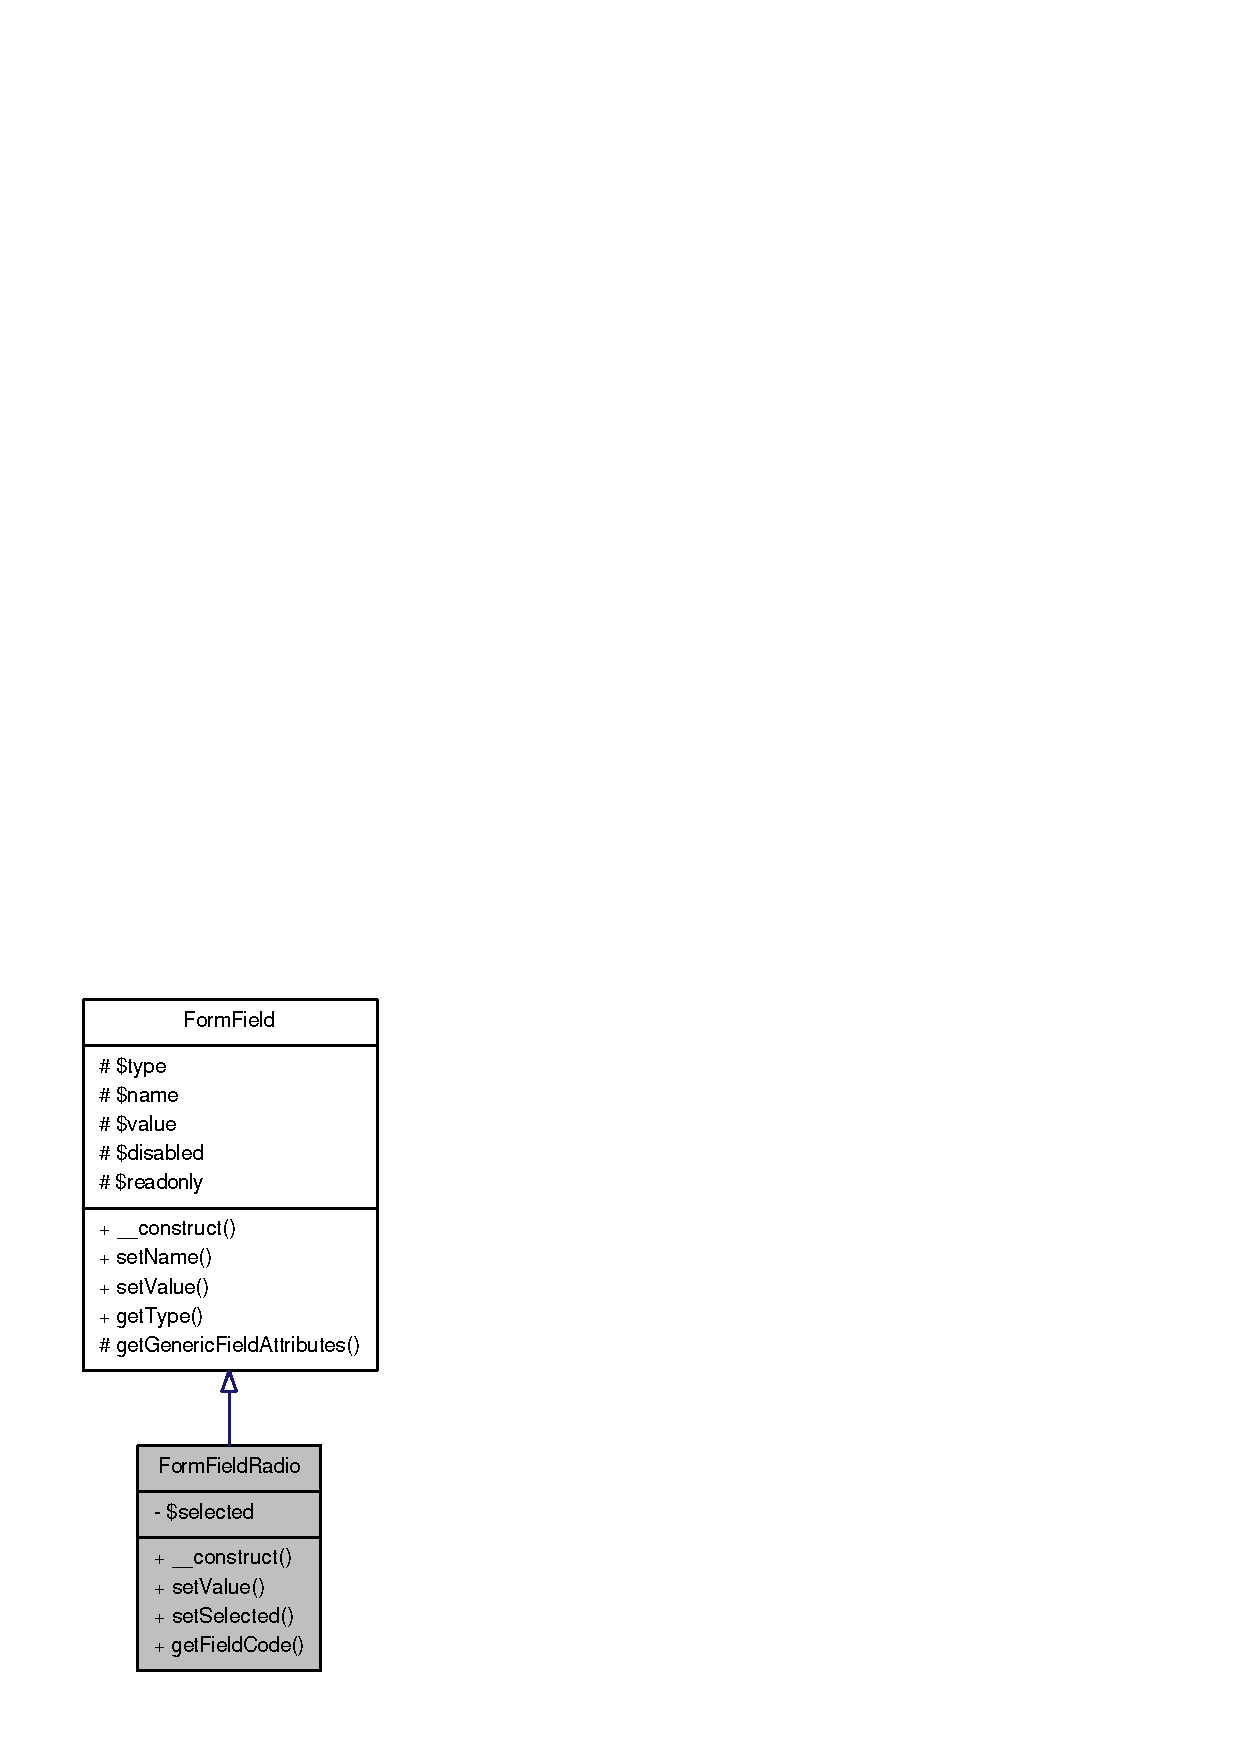
\includegraphics[width=184pt]{classFormFieldRadio__inherit__graph}
\end{center}
\end{figure}


Collaboration diagram for FormFieldRadio:\nopagebreak
\begin{figure}[H]
\begin{center}
\leavevmode
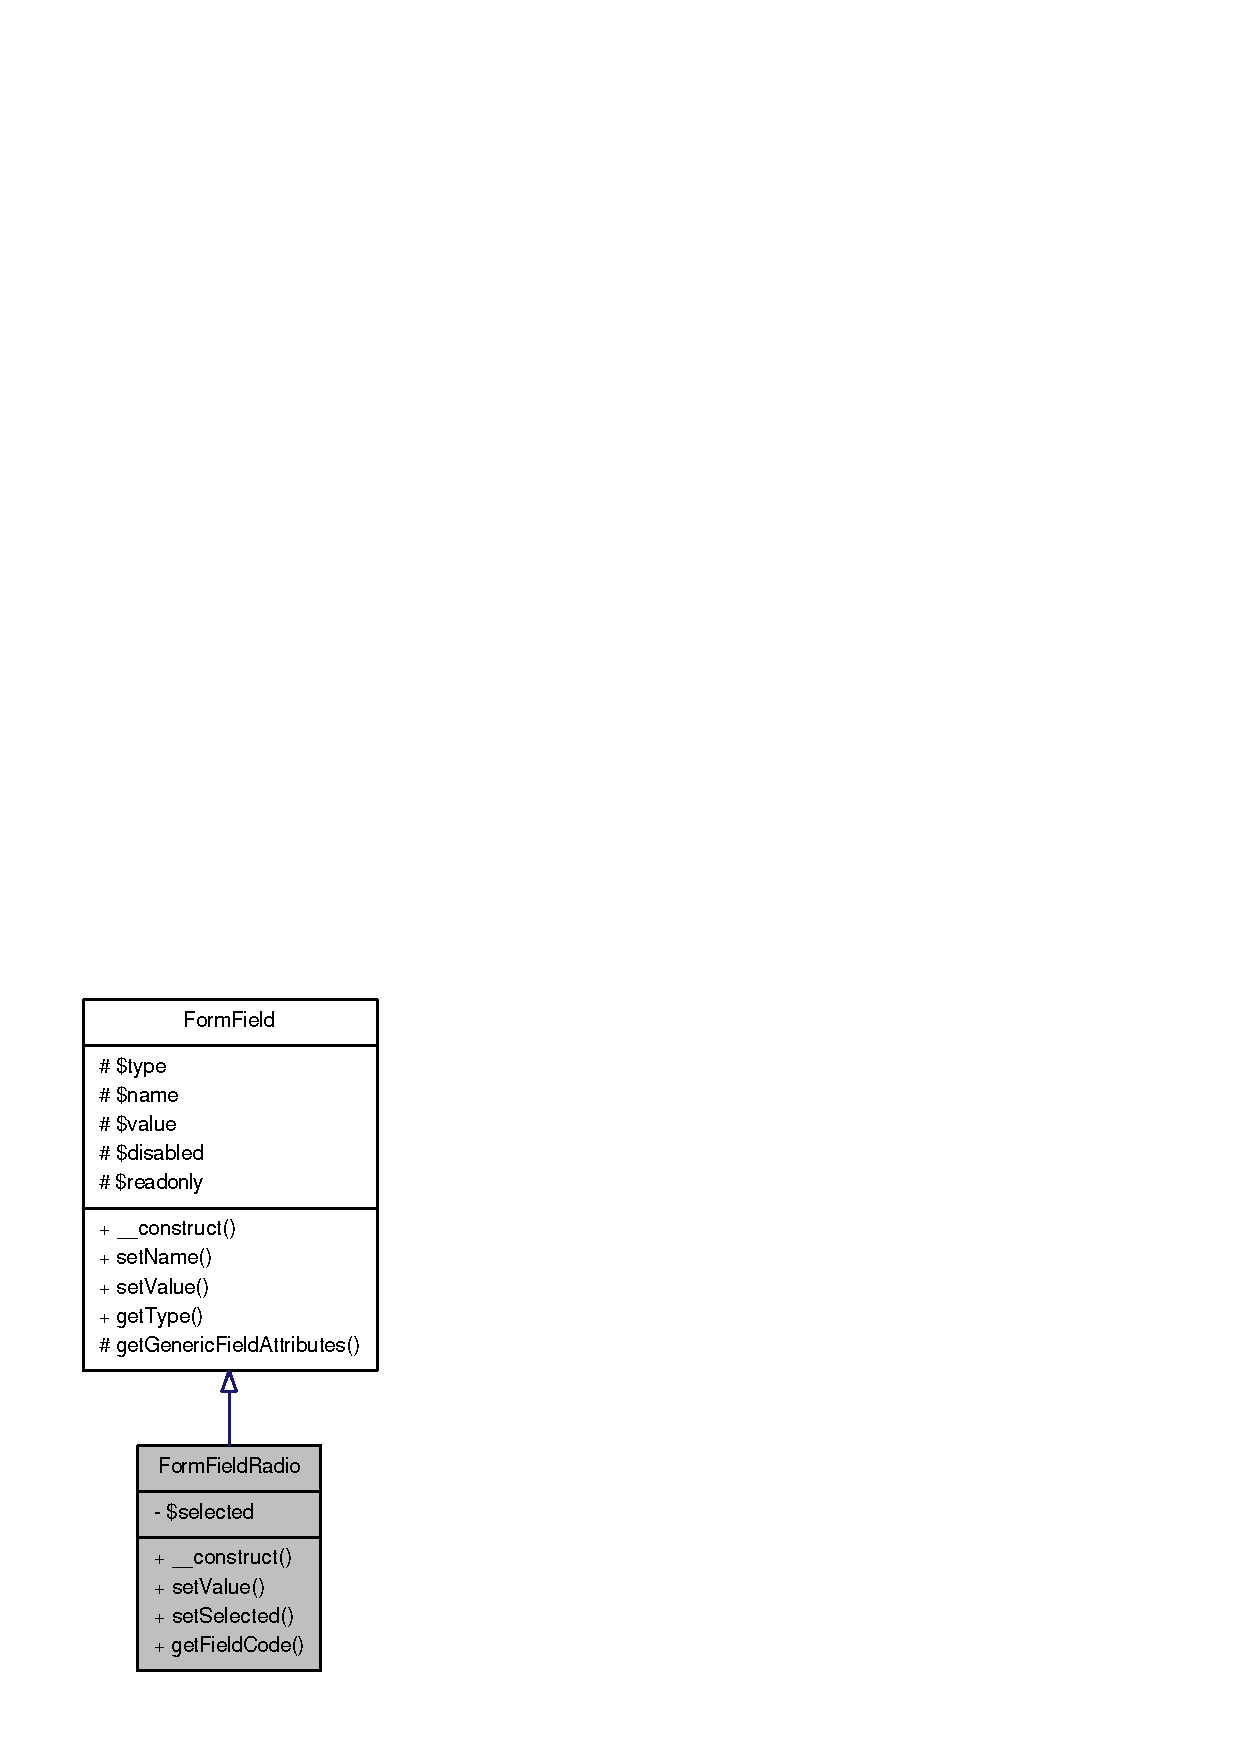
\includegraphics[width=184pt]{classFormFieldRadio__coll__graph}
\end{center}
\end{figure}
\subsection*{Public Member Functions}
\begin{DoxyCompactItemize}
\item 
\hyperlink{classFormFieldRadio_ae82224cf68e3513e29923c24f42eb06d}{\_\-\_\-construct} ()
\item 
\hyperlink{classFormFieldRadio_aab105e92866fd80890d3254f51a2e4ca}{setValue} (\$\_\-value)
\item 
\hyperlink{classFormFieldRadio_a2fc7c97f763930e5bdd8f7cbb7f3c98f}{setSelected} (\$\_\-value)
\item 
\hyperlink{classFormFieldRadio_a727e6c7c77ed0e2b49108d0e44c6e8d3}{getFieldCode} ()
\item 
\hyperlink{classFormField_ad57e32bd53170af060e869b3b60f0ef7}{setName} (\$\_\-value)
\item 
\hyperlink{classFormField_a1f64b737bccb6b2827f8c5665b9920c7}{getType} ()
\end{DoxyCompactItemize}
\subsection*{Protected Member Functions}
\begin{DoxyCompactItemize}
\item 
\hyperlink{classFormField_a9f9d136ba8b4a793f22370aff43d592d}{getGenericFieldAttributes} (\$\_\-ignore=array())
\end{DoxyCompactItemize}
\subsection*{Protected Attributes}
\begin{DoxyCompactItemize}
\item 
\hyperlink{classFormField_a37bed21a1891e95be0e4a697e45ba51b}{\$type}
\item 
\hyperlink{classFormField_a23861f707bcd77bbace6300de9621746}{\$name}
\item 
\hyperlink{classFormField_a3c01e89834248eec8e2f145fbcfa0fbc}{\$value}
\item 
\hyperlink{classFormField_ab6f1907061890290e32cb2befc0a5f50}{\$disabled}
\item 
\hyperlink{classFormField_a78ba5d4b9127e75e8ccf86f397b5d9ac}{\$readonly}
\end{DoxyCompactItemize}
\subsection*{Private Attributes}
\begin{DoxyCompactItemize}
\item 
\hyperlink{classFormFieldRadio_a1b6abf4c527efabf94d2b5147492007e}{\$selected}
\end{DoxyCompactItemize}


\subsection{Detailed Description}
Formfield. Formfield radio elements \begin{DoxyAuthor}{Author}
Oscar van Eijk, Oveas Functionality Provider 
\end{DoxyAuthor}
\begin{DoxyVersion}{Version}
Oct 19, 2010 -\/-\/ O van Eijk -\/-\/ initial version 
\end{DoxyVersion}


\subsection{Constructor \& Destructor Documentation}
\index{FormFieldRadio@{FormFieldRadio}!\_\-\_\-construct@{\_\-\_\-construct}}
\index{\_\-\_\-construct@{\_\-\_\-construct}!FormFieldRadio@{FormFieldRadio}}
\subsubsection[{\_\-\_\-construct}]{\setlength{\rightskip}{0pt plus 5cm}FormFieldRadio::\_\-\_\-construct ()}\label{classFormFieldRadio_ae82224cf68e3513e29923c24f42eb06d}
Class constructor; 

Reimplemented from \hyperlink{classFormField_a0cfe713ce28a6a0cb53476ed463e1f01}{FormField}.



\subsection{Member Function Documentation}
\index{FormFieldRadio@{FormFieldRadio}!getFieldCode@{getFieldCode}}
\index{getFieldCode@{getFieldCode}!FormFieldRadio@{FormFieldRadio}}
\subsubsection[{getFieldCode}]{\setlength{\rightskip}{0pt plus 5cm}FormFieldRadio::getFieldCode ()}\label{classFormFieldRadio_a727e6c7c77ed0e2b49108d0e44c6e8d3}
Return the HTML code to display the form elements

\begin{DoxyReturn}{Returns}
Array with textstrings for each radio button in this this set. 
\end{DoxyReturn}


References FormField::getGenericFieldAttributes().

\index{FormFieldRadio@{FormFieldRadio}!getGenericFieldAttributes@{getGenericFieldAttributes}}
\index{getGenericFieldAttributes@{getGenericFieldAttributes}!FormFieldRadio@{FormFieldRadio}}
\subsubsection[{getGenericFieldAttributes}]{\setlength{\rightskip}{0pt plus 5cm}FormField::getGenericFieldAttributes (\$ {\em \_\-ignore} = {\ttfamily array()})\hspace{0.3cm}{\ttfamily  \mbox{[}protected, inherited\mbox{]}}}\label{classFormField_a9f9d136ba8b4a793f22370aff43d592d}
Return the attributes for an HTML formfield in the \char`\"{} attrib='value' \mbox{[}...\mbox{]}\char`\"{} format


\begin{DoxyParams}{Parameters}
\item[\mbox{$\leftarrow$} {\em \$\_\-ignore}]Array with attributes names that should be ignored, e.g. for a textarea, the value is not returned as an attribute. \end{DoxyParams}
\begin{DoxyReturn}{Returns}
Textstring with the HTML code 
\end{DoxyReturn}


Referenced by FormFieldTextarea::getFieldCode(), FormFieldText::getFieldCode(), getFieldCode(), FormFieldCheckbox::getFieldCode(), and FormFieldButton::getFieldCode().

\index{FormFieldRadio@{FormFieldRadio}!getType@{getType}}
\index{getType@{getType}!FormFieldRadio@{FormFieldRadio}}
\subsubsection[{getType}]{\setlength{\rightskip}{0pt plus 5cm}FormField::getType ()\hspace{0.3cm}{\ttfamily  \mbox{[}inherited\mbox{]}}}\label{classFormField_a1f64b737bccb6b2827f8c5665b9920c7}
Give the field type \begin{DoxyReturn}{Returns}
Field type 
\end{DoxyReturn}
\index{FormFieldRadio@{FormFieldRadio}!setName@{setName}}
\index{setName@{setName}!FormFieldRadio@{FormFieldRadio}}
\subsubsection[{setName}]{\setlength{\rightskip}{0pt plus 5cm}FormField::setName (\$ {\em \_\-value})\hspace{0.3cm}{\ttfamily  \mbox{[}inherited\mbox{]}}}\label{classFormField_ad57e32bd53170af060e869b3b60f0ef7}
Set the field name 
\begin{DoxyParams}{Parameters}
\item[\mbox{$\leftarrow$} {\em \$\_\-value}]Field name \end{DoxyParams}
\index{FormFieldRadio@{FormFieldRadio}!setSelected@{setSelected}}
\index{setSelected@{setSelected}!FormFieldRadio@{FormFieldRadio}}
\subsubsection[{setSelected}]{\setlength{\rightskip}{0pt plus 5cm}FormFieldRadio::setSelected (\$ {\em \_\-value})}\label{classFormFieldRadio_a2fc7c97f763930e5bdd8f7cbb7f3c98f}
Define the selected value 
\begin{DoxyParams}{Parameters}
\item[\mbox{$\leftarrow$} {\em \$\_\-value}]Preselected value \end{DoxyParams}
\index{FormFieldRadio@{FormFieldRadio}!setValue@{setValue}}
\index{setValue@{setValue}!FormFieldRadio@{FormFieldRadio}}
\subsubsection[{setValue}]{\setlength{\rightskip}{0pt plus 5cm}FormFieldRadio::setValue (\$ {\em \_\-value})}\label{classFormFieldRadio_aab105e92866fd80890d3254f51a2e4ca}
Reimplement, multiple values are supported 
\begin{DoxyParams}{Parameters}
\item[\mbox{$\leftarrow$} {\em \$\_\-value}]Field value \end{DoxyParams}


Reimplemented from \hyperlink{classFormField_a465ff61e290d82be96bb793c3a14b3e7}{FormField}.



\subsection{Member Data Documentation}
\index{FormFieldRadio@{FormFieldRadio}!\$disabled@{\$disabled}}
\index{\$disabled@{\$disabled}!FormFieldRadio@{FormFieldRadio}}
\subsubsection[{\$disabled}]{\setlength{\rightskip}{0pt plus 5cm}FormField::\$disabled\hspace{0.3cm}{\ttfamily  \mbox{[}protected, inherited\mbox{]}}}\label{classFormField_ab6f1907061890290e32cb2befc0a5f50}
Boolean indicating a disabled field when true \index{FormFieldRadio@{FormFieldRadio}!\$name@{\$name}}
\index{\$name@{\$name}!FormFieldRadio@{FormFieldRadio}}
\subsubsection[{\$name}]{\setlength{\rightskip}{0pt plus 5cm}FormField::\$name\hspace{0.3cm}{\ttfamily  \mbox{[}protected, inherited\mbox{]}}}\label{classFormField_a23861f707bcd77bbace6300de9621746}
Name of the formfield \index{FormFieldRadio@{FormFieldRadio}!\$readonly@{\$readonly}}
\index{\$readonly@{\$readonly}!FormFieldRadio@{FormFieldRadio}}
\subsubsection[{\$readonly}]{\setlength{\rightskip}{0pt plus 5cm}FormField::\$readonly\hspace{0.3cm}{\ttfamily  \mbox{[}protected, inherited\mbox{]}}}\label{classFormField_a78ba5d4b9127e75e8ccf86f397b5d9ac}
Boolean indicating a readonly field when true \index{FormFieldRadio@{FormFieldRadio}!\$selected@{\$selected}}
\index{\$selected@{\$selected}!FormFieldRadio@{FormFieldRadio}}
\subsubsection[{\$selected}]{\setlength{\rightskip}{0pt plus 5cm}FormFieldRadio::\$selected\hspace{0.3cm}{\ttfamily  \mbox{[}private\mbox{]}}}\label{classFormFieldRadio_a1b6abf4c527efabf94d2b5147492007e}
Holds the value that must be preselected \index{FormFieldRadio@{FormFieldRadio}!\$type@{\$type}}
\index{\$type@{\$type}!FormFieldRadio@{FormFieldRadio}}
\subsubsection[{\$type}]{\setlength{\rightskip}{0pt plus 5cm}FormField::\$type\hspace{0.3cm}{\ttfamily  \mbox{[}protected, inherited\mbox{]}}}\label{classFormField_a37bed21a1891e95be0e4a697e45ba51b}
Field type 

Reimplemented in \hyperlink{classFormFieldTextarea_a85348034822c70694fc8640bfcacc04d}{FormFieldTextarea}.



Referenced by FormFieldText::\_\-\_\-construct(), and FormFieldButton::\_\-\_\-construct().

\index{FormFieldRadio@{FormFieldRadio}!\$value@{\$value}}
\index{\$value@{\$value}!FormFieldRadio@{FormFieldRadio}}
\subsubsection[{\$value}]{\setlength{\rightskip}{0pt plus 5cm}FormField::\$value\hspace{0.3cm}{\ttfamily  \mbox{[}protected, inherited\mbox{]}}}\label{classFormField_a3c01e89834248eec8e2f145fbcfa0fbc}
Field value 

The documentation for this class was generated from the following file:\begin{DoxyCompactItemize}
\item 
/home/oscar/projects/owl-\/php/src/kernel/ui/\hyperlink{class_8formfield_8radio_8php}{class.formfield.radio.php}\end{DoxyCompactItemize}

\section{FormFieldSelect Class Reference}
\label{classFormFieldSelect}\index{FormFieldSelect@{FormFieldSelect}}


Formfield.  




Inheritance diagram for FormFieldSelect:\nopagebreak
\begin{figure}[H]
\begin{center}
\leavevmode
\includegraphics[width=184pt]{classFormFieldSelect__inherit__graph}
\end{center}
\end{figure}


Collaboration diagram for FormFieldSelect:\nopagebreak
\begin{figure}[H]
\begin{center}
\leavevmode
\includegraphics[width=184pt]{classFormFieldSelect__coll__graph}
\end{center}
\end{figure}
\subsection*{Public Member Functions}
\begin{DoxyCompactItemize}
\item 
\hyperlink{classFormFieldSelect_a32c59192be8c316fb2f7e1edde8f0a98}{\_\-\_\-construct} ()
\item 
\hyperlink{classFormFieldSelect_ae69f5b352df63796c048dca6a2de7544}{setValue} (\$\_\-value)
\item 
\hyperlink{classFormFieldSelect_ad8ae8dcf6f6763cb32966eeca33c472b}{setSize} (\$size)
\item 
\hyperlink{classFormFieldSelect_aa69374c1f0692d691e7899f3ed14a42e}{setMultiple} (\$\_\-value=true)
\item 
\hyperlink{classFormField_ad57e32bd53170af060e869b3b60f0ef7}{setName} (\$\_\-value)
\item 
\hyperlink{classFormField_a1f64b737bccb6b2827f8c5665b9920c7}{getType} ()
\end{DoxyCompactItemize}
\subsection*{Protected Member Functions}
\begin{DoxyCompactItemize}
\item 
\hyperlink{classFormField_a9f9d136ba8b4a793f22370aff43d592d}{getGenericFieldAttributes} (\$\_\-ignore=array())
\end{DoxyCompactItemize}
\subsection*{Protected Attributes}
\begin{DoxyCompactItemize}
\item 
\hyperlink{classFormField_a37bed21a1891e95be0e4a697e45ba51b}{\$type}
\item 
\hyperlink{classFormField_a23861f707bcd77bbace6300de9621746}{\$name}
\item 
\hyperlink{classFormField_a3c01e89834248eec8e2f145fbcfa0fbc}{\$value}
\item 
\hyperlink{classFormField_ab6f1907061890290e32cb2befc0a5f50}{\$disabled}
\item 
\hyperlink{classFormField_a78ba5d4b9127e75e8ccf86f397b5d9ac}{\$readonly}
\end{DoxyCompactItemize}
\subsection*{Private Attributes}
\begin{DoxyCompactItemize}
\item 
\hyperlink{classFormFieldSelect_a8e79d63b2f69dc06959f3f0dc6f0a12a}{\$size}
\item 
\hyperlink{classFormFieldSelect_a6eb8f177d1cfd20845509c0a35120725}{\$multiple}
\item 
\hyperlink{classFormFieldSelect_a5c4b74ae8d7274e642e78e5a514c9736}{\$options}
\end{DoxyCompactItemize}


\subsection{Detailed Description}
Formfield. Formfield selectlist elements \begin{DoxyAuthor}{Author}
Oscar van Eijk, Oveas Functionality Provider 
\end{DoxyAuthor}
\begin{DoxyVersion}{Version}
Oct 19, 2010 -\/-\/ O van Eijk -\/-\/ initial version 
\end{DoxyVersion}


\subsection{Constructor \& Destructor Documentation}
\index{FormFieldSelect@{FormFieldSelect}!\_\-\_\-construct@{\_\-\_\-construct}}
\index{\_\-\_\-construct@{\_\-\_\-construct}!FormFieldSelect@{FormFieldSelect}}
\subsubsection[{\_\-\_\-construct}]{\setlength{\rightskip}{0pt plus 5cm}FormFieldSelect::\_\-\_\-construct ()}\label{classFormFieldSelect_a32c59192be8c316fb2f7e1edde8f0a98}
Class constructor; 

Reimplemented from \hyperlink{classFormField_a0cfe713ce28a6a0cb53476ed463e1f01}{FormField}.



\subsection{Member Function Documentation}
\index{FormFieldSelect@{FormFieldSelect}!getGenericFieldAttributes@{getGenericFieldAttributes}}
\index{getGenericFieldAttributes@{getGenericFieldAttributes}!FormFieldSelect@{FormFieldSelect}}
\subsubsection[{getGenericFieldAttributes}]{\setlength{\rightskip}{0pt plus 5cm}FormField::getGenericFieldAttributes (\$ {\em \_\-ignore} = {\ttfamily array()})\hspace{0.3cm}{\ttfamily  \mbox{[}protected, inherited\mbox{]}}}\label{classFormField_a9f9d136ba8b4a793f22370aff43d592d}
Return the attributes for an HTML formfield in the \char`\"{} attrib='value' \mbox{[}...\mbox{]}\char`\"{} format


\begin{DoxyParams}{Parameters}
\item[\mbox{$\leftarrow$} {\em \$\_\-ignore}]Array with attributes names that should be ignored, e.g. for a textarea, the value is not returned as an attribute. \end{DoxyParams}
\begin{DoxyReturn}{Returns}
Textstring with the HTML code 
\end{DoxyReturn}


Referenced by FormFieldTextarea::getFieldCode(), FormFieldText::getFieldCode(), FormFieldRadio::getFieldCode(), FormFieldCheckbox::getFieldCode(), and FormFieldButton::getFieldCode().

\index{FormFieldSelect@{FormFieldSelect}!getType@{getType}}
\index{getType@{getType}!FormFieldSelect@{FormFieldSelect}}
\subsubsection[{getType}]{\setlength{\rightskip}{0pt plus 5cm}FormField::getType ()\hspace{0.3cm}{\ttfamily  \mbox{[}inherited\mbox{]}}}\label{classFormField_a1f64b737bccb6b2827f8c5665b9920c7}
Give the field type \begin{DoxyReturn}{Returns}
Field type 
\end{DoxyReturn}
\index{FormFieldSelect@{FormFieldSelect}!setMultiple@{setMultiple}}
\index{setMultiple@{setMultiple}!FormFieldSelect@{FormFieldSelect}}
\subsubsection[{setMultiple}]{\setlength{\rightskip}{0pt plus 5cm}FormFieldSelect::setMultiple (\$ {\em \_\-value} = {\ttfamily true})}\label{classFormFieldSelect_aa69374c1f0692d691e7899f3ed14a42e}
Set the Multiple boolean 
\begin{DoxyParams}{Parameters}
\item[\mbox{$\leftarrow$} {\em \$\_\-value}]Value indicating true (default) or false \end{DoxyParams}
\index{FormFieldSelect@{FormFieldSelect}!setName@{setName}}
\index{setName@{setName}!FormFieldSelect@{FormFieldSelect}}
\subsubsection[{setName}]{\setlength{\rightskip}{0pt plus 5cm}FormField::setName (\$ {\em \_\-value})\hspace{0.3cm}{\ttfamily  \mbox{[}inherited\mbox{]}}}\label{classFormField_ad57e32bd53170af060e869b3b60f0ef7}
Set the field name 
\begin{DoxyParams}{Parameters}
\item[\mbox{$\leftarrow$} {\em \$\_\-value}]Field name \end{DoxyParams}
\index{FormFieldSelect@{FormFieldSelect}!setSize@{setSize}}
\index{setSize@{setSize}!FormFieldSelect@{FormFieldSelect}}
\subsubsection[{setSize}]{\setlength{\rightskip}{0pt plus 5cm}FormFieldSelect::setSize (\$ {\em size})}\label{classFormFieldSelect_ad8ae8dcf6f6763cb32966eeca33c472b}
Set the Size attribute 
\begin{DoxyParams}{Parameters}
\item[\mbox{$\leftarrow$} {\em \$size}]integer \end{DoxyParams}


References \$size.

\index{FormFieldSelect@{FormFieldSelect}!setValue@{setValue}}
\index{setValue@{setValue}!FormFieldSelect@{FormFieldSelect}}
\subsubsection[{setValue}]{\setlength{\rightskip}{0pt plus 5cm}FormFieldSelect::setValue (\$ {\em \_\-value})}\label{classFormFieldSelect_ae69f5b352df63796c048dca6a2de7544}
Define the options 
\begin{DoxyParams}{Parameters}
\item[\mbox{$\leftarrow$} {\em \$\_\-value}]2-\/Dimensional array with option data. The first level contains indexed arrays with data for each option in the format: 
\begin{DoxyCode}
 array (
     'value' => string // Required, value that will be submitted
    ,'text'  => string // Optional, text that will be displayed, defaults to 'val
      ue'
    ,'class' => string // Optional, class name
    ,'group' => string // Optional, label of the optgroup the option belongs to
 )
\end{DoxyCode}
 \end{DoxyParams}


Reimplemented from \hyperlink{classFormField_a465ff61e290d82be96bb793c3a14b3e7}{FormField}.



\subsection{Member Data Documentation}
\index{FormFieldSelect@{FormFieldSelect}!\$disabled@{\$disabled}}
\index{\$disabled@{\$disabled}!FormFieldSelect@{FormFieldSelect}}
\subsubsection[{\$disabled}]{\setlength{\rightskip}{0pt plus 5cm}FormField::\$disabled\hspace{0.3cm}{\ttfamily  \mbox{[}protected, inherited\mbox{]}}}\label{classFormField_ab6f1907061890290e32cb2befc0a5f50}
Boolean indicating a disabled field when true \index{FormFieldSelect@{FormFieldSelect}!\$multiple@{\$multiple}}
\index{\$multiple@{\$multiple}!FormFieldSelect@{FormFieldSelect}}
\subsubsection[{\$multiple}]{\setlength{\rightskip}{0pt plus 5cm}FormFieldSelect::\$multiple\hspace{0.3cm}{\ttfamily  \mbox{[}private\mbox{]}}}\label{classFormFieldSelect_a6eb8f177d1cfd20845509c0a35120725}
Boolean indicating a multiple select \index{FormFieldSelect@{FormFieldSelect}!\$name@{\$name}}
\index{\$name@{\$name}!FormFieldSelect@{FormFieldSelect}}
\subsubsection[{\$name}]{\setlength{\rightskip}{0pt plus 5cm}FormField::\$name\hspace{0.3cm}{\ttfamily  \mbox{[}protected, inherited\mbox{]}}}\label{classFormField_a23861f707bcd77bbace6300de9621746}
Name of the formfield \index{FormFieldSelect@{FormFieldSelect}!\$options@{\$options}}
\index{\$options@{\$options}!FormFieldSelect@{FormFieldSelect}}
\subsubsection[{\$options}]{\setlength{\rightskip}{0pt plus 5cm}FormFieldSelect::\$options\hspace{0.3cm}{\ttfamily  \mbox{[}private\mbox{]}}}\label{classFormFieldSelect_a5c4b74ae8d7274e642e78e5a514c9736}
Array with options for the select list \index{FormFieldSelect@{FormFieldSelect}!\$readonly@{\$readonly}}
\index{\$readonly@{\$readonly}!FormFieldSelect@{FormFieldSelect}}
\subsubsection[{\$readonly}]{\setlength{\rightskip}{0pt plus 5cm}FormField::\$readonly\hspace{0.3cm}{\ttfamily  \mbox{[}protected, inherited\mbox{]}}}\label{classFormField_a78ba5d4b9127e75e8ccf86f397b5d9ac}
Boolean indicating a readonly field when true \index{FormFieldSelect@{FormFieldSelect}!\$size@{\$size}}
\index{\$size@{\$size}!FormFieldSelect@{FormFieldSelect}}
\subsubsection[{\$size}]{\setlength{\rightskip}{0pt plus 5cm}FormFieldSelect::\$size\hspace{0.3cm}{\ttfamily  \mbox{[}private\mbox{]}}}\label{classFormFieldSelect_a8e79d63b2f69dc06959f3f0dc6f0a12a}
Number of visible options 

Referenced by setSize().

\index{FormFieldSelect@{FormFieldSelect}!\$type@{\$type}}
\index{\$type@{\$type}!FormFieldSelect@{FormFieldSelect}}
\subsubsection[{\$type}]{\setlength{\rightskip}{0pt plus 5cm}FormField::\$type\hspace{0.3cm}{\ttfamily  \mbox{[}protected, inherited\mbox{]}}}\label{classFormField_a37bed21a1891e95be0e4a697e45ba51b}
Field type 

Reimplemented in \hyperlink{classFormFieldTextarea_a85348034822c70694fc8640bfcacc04d}{FormFieldTextarea}.



Referenced by FormFieldText::\_\-\_\-construct(), and FormFieldButton::\_\-\_\-construct().

\index{FormFieldSelect@{FormFieldSelect}!\$value@{\$value}}
\index{\$value@{\$value}!FormFieldSelect@{FormFieldSelect}}
\subsubsection[{\$value}]{\setlength{\rightskip}{0pt plus 5cm}FormField::\$value\hspace{0.3cm}{\ttfamily  \mbox{[}protected, inherited\mbox{]}}}\label{classFormField_a3c01e89834248eec8e2f145fbcfa0fbc}
Field value 

The documentation for this class was generated from the following file:\begin{DoxyCompactItemize}
\item 
/home/oscar/projects/owl-\/php/src/kernel/ui/\hyperlink{class_8formfield_8select_8php}{class.formfield.select.php}\end{DoxyCompactItemize}

\section{FormFieldText Class Reference}
\label{classFormFieldText}\index{FormFieldText@{FormFieldText}}


Formfield.  




Inheritance diagram for FormFieldText:\nopagebreak
\begin{figure}[H]
\begin{center}
\leavevmode
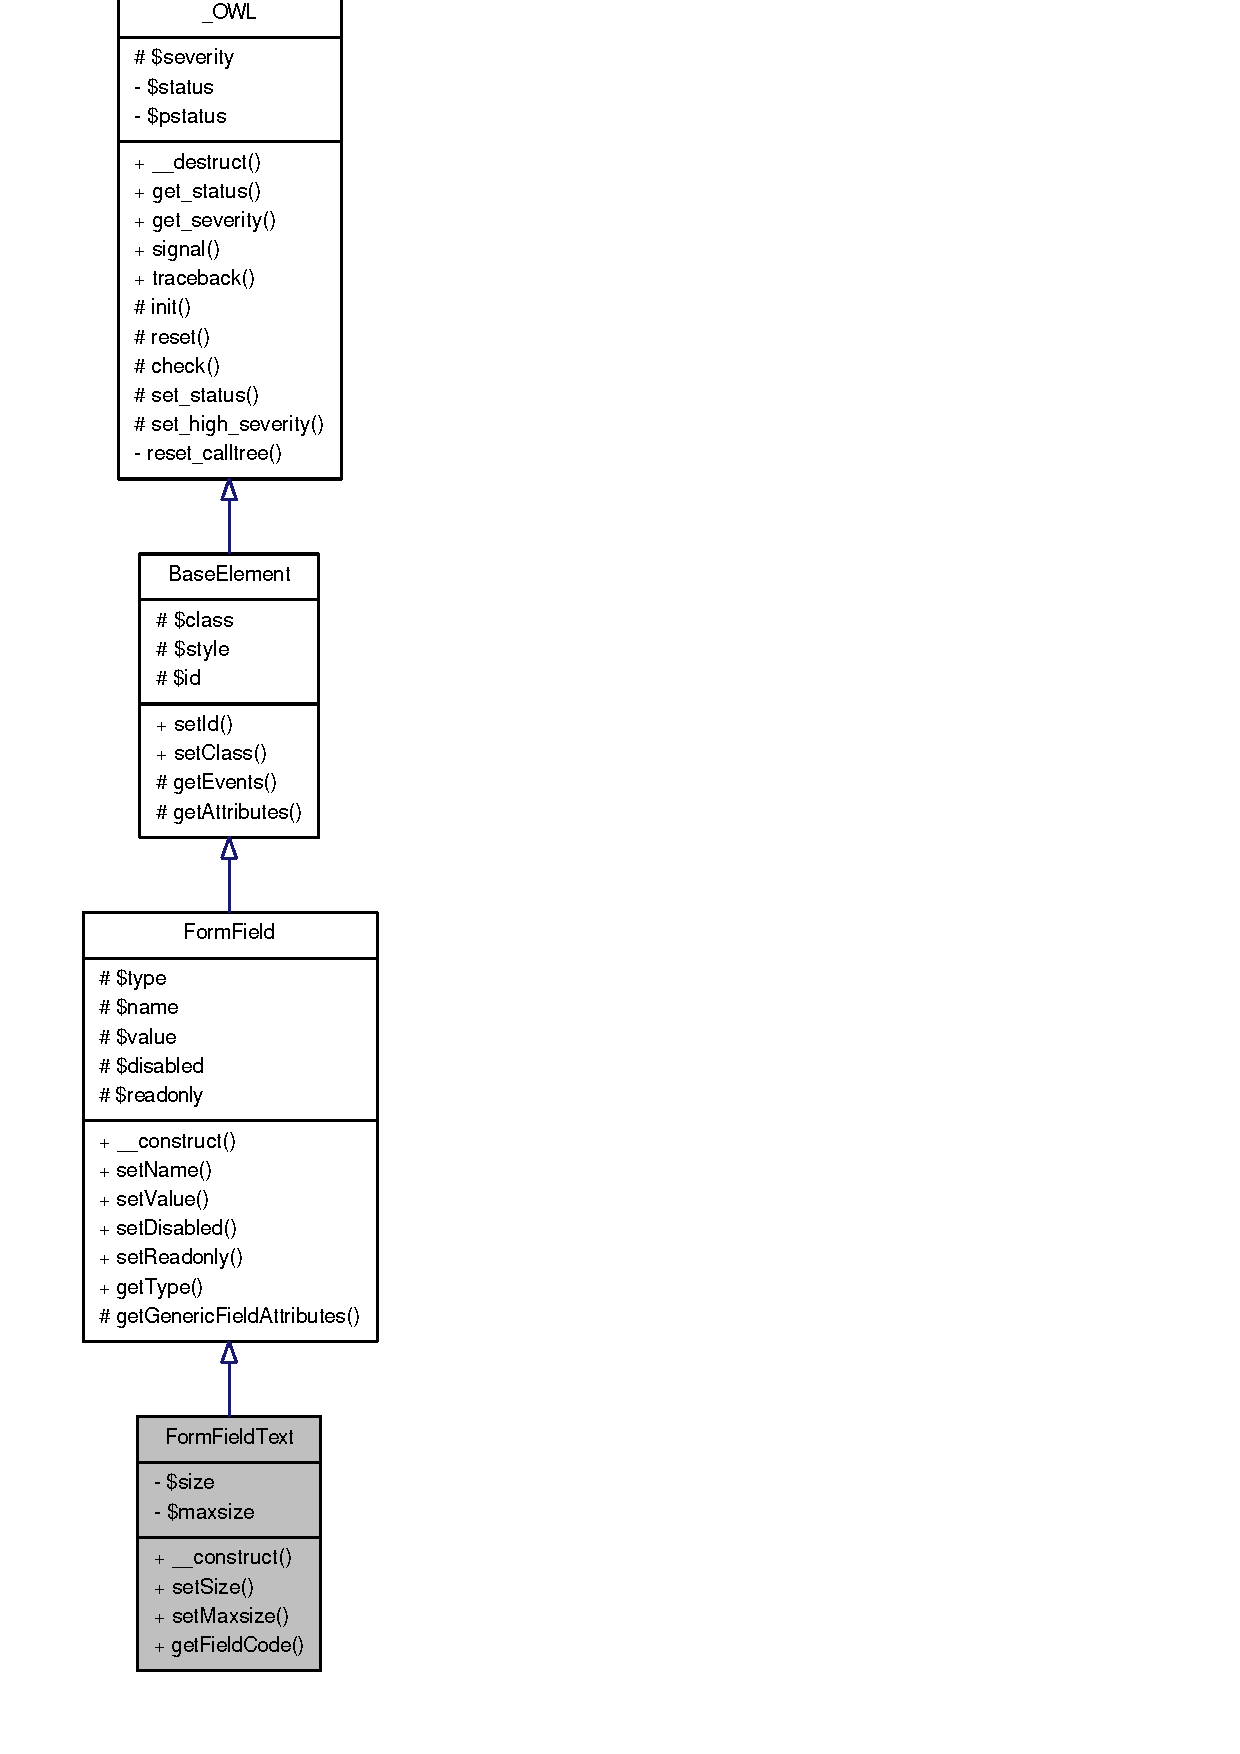
\includegraphics[height=600pt]{classFormFieldText__inherit__graph}
\end{center}
\end{figure}


Collaboration diagram for FormFieldText:\nopagebreak
\begin{figure}[H]
\begin{center}
\leavevmode
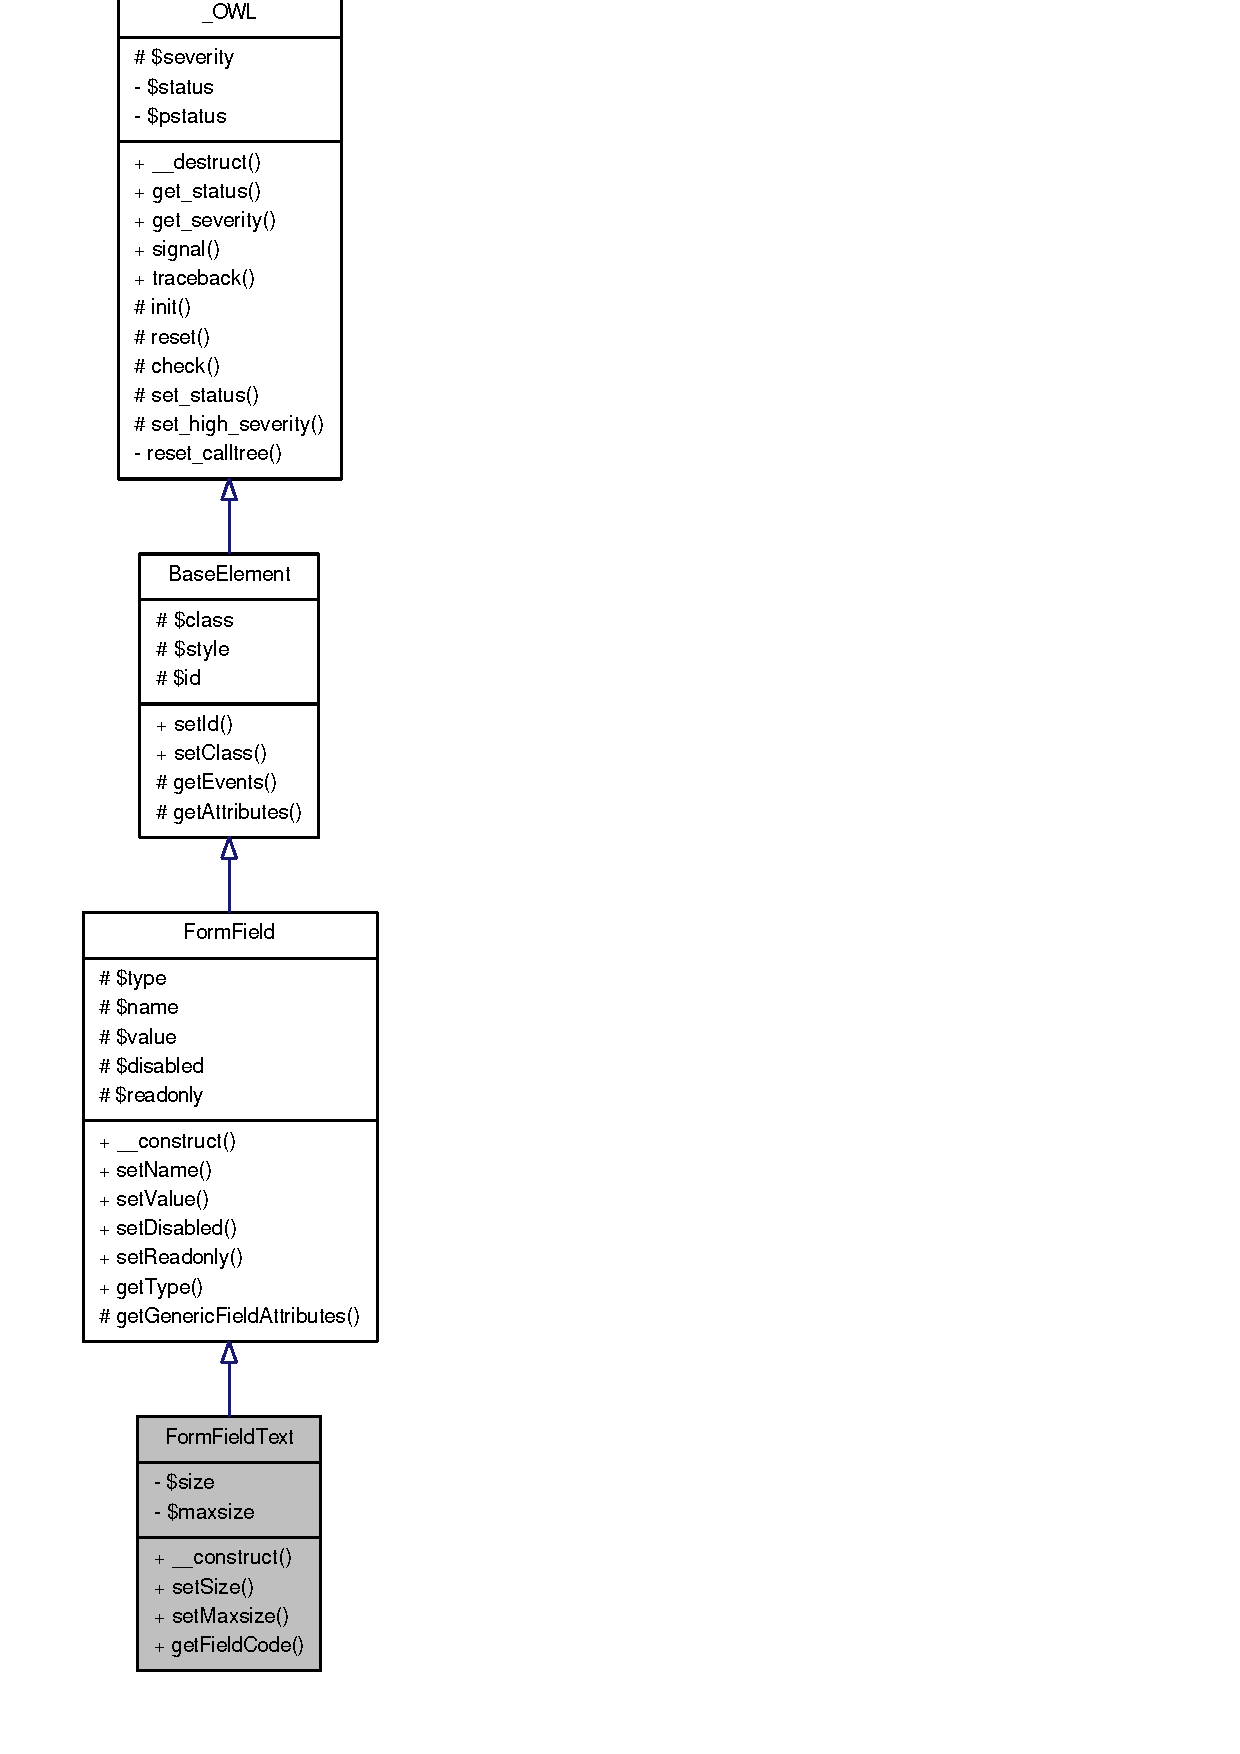
\includegraphics[height=600pt]{classFormFieldText__coll__graph}
\end{center}
\end{figure}
\subsection*{Public Member Functions}
\begin{DoxyCompactItemize}
\item 
\hyperlink{classFormFieldText_a19f605d6195d340c6ddf9a298706b9cd}{\_\-\_\-construct} (\$type= 'text')
\item 
\hyperlink{classFormFieldText_a045b0853ed6e7777c7f3dddbadf31f5f}{setSize} (\$size)
\item 
\hyperlink{classFormFieldText_a91b6ce8a3476c4296fbe1b0802e70984}{setMaxsize} (\$maxsize)
\item 
\hyperlink{classFormFieldText_aebbf56aba1fd099619a360ac259633fa}{getFieldCode} ()
\item 
\hyperlink{classFormField_a465ff61e290d82be96bb793c3a14b3e7}{setValue} (\$\_\-value)
\item 
\hyperlink{classFormField_a9fa2c828eaf98154edfaa2e755657117}{setDisabled} (\$\_\-value=true)
\item 
\hyperlink{classFormField_a6eabbb35d24b1698ea25b66ddfd88a64}{setReadonly} (\$\_\-value=true)
\item 
\hyperlink{classFormField_a1f64b737bccb6b2827f8c5665b9920c7}{getType} ()
\item 
\hyperlink{classBaseElement_a0c1ce3d1684ecb78960cf7a97278494e}{setId} (\$\_\-value)
\item 
\hyperlink{classBaseElement_a39bafb3609d10048920c20242c2a04c5}{setName} (\$\_\-value)
\item 
\hyperlink{classBaseElement_a6b2b9ff69f6e92db82f91d9c55cda697}{setStyle} (\$\_\-value)
\item 
\hyperlink{classBaseElement_af6597b30fa9798878f6290271043dfa2}{setClass} (\$\_\-value)
\item 
\hyperlink{classBaseElement_ad5789f45f16aaa144716ee8558069c31}{setEvent} (\$\_\-event, \$\_\-action, \$\_\-add=false)
\item 
\hyperlink{class__OWL_a99ec771fa2c5c279f80152cc09e489a8}{get\_\-status} ()
\item 
\hyperlink{class__OWL_adf9509ef96858be7bdd9414c5ef129aa}{get\_\-severity} (\$status=null)
\item 
\hyperlink{class__OWL_a51ba4a16409acf2a2f61f286939091a5}{signal} (\$level=\hyperlink{owl_8severitycodes_8php_a139328861128689f2f4def6a399d9057}{OWL\_\-INFO}, \&\$text=false)
\item 
\hyperlink{class__OWL_aa29547995d6741b7d2b90c1d4ea99a13}{traceback} (\&\$text=false, \$depth=0)
\end{DoxyCompactItemize}
\subsection*{Protected Member Functions}
\begin{DoxyCompactItemize}
\item 
\hyperlink{classFormField_a9f9d136ba8b4a793f22370aff43d592d}{getGenericFieldAttributes} (\$\_\-ignore=array())
\item 
\hyperlink{classBaseElement_aa623b042d23a5b77add8b3c452ec5855}{setAttributes} (\$\_\-attribs)
\item 
\hyperlink{classBaseElement_ae8237038633fc53db818f36da1940297}{getAttributes} (\$\_\-ignore=array())
\item 
\hyperlink{class__OWL_ae0ef3ded56e8a6b34b6461e5a721cd3e}{init} ()
\item 
\hyperlink{class__OWL_a2f2a042bcf31965194c03033df0edc9b}{reset} ()
\item 
\hyperlink{class__OWL_a9e49b9c76fbc021b244c6915ea536d71}{save\_\-status} ()
\item 
\hyperlink{class__OWL_a465eeaf40edd9f9c848841700c32ce55}{restore\_\-status} ()
\item 
\hyperlink{class__OWL_ad6f4f6946f40199dd0333cf219fa500e}{check} (\&\$object, \$level)
\item 
\hyperlink{class__OWL_aea912d0ede9b3c2a69b79072d94d4787}{set\_\-status} (\$status, \$params=array())
\item 
\hyperlink{class__OWL_a576829692a3b66e3d518853bf43abae3}{set\_\-high\_\-severity} (\&\$object=null)
\end{DoxyCompactItemize}
\subsection*{Protected Attributes}
\begin{DoxyCompactItemize}
\item 
\hyperlink{classFormField_a37bed21a1891e95be0e4a697e45ba51b}{\$type}
\item 
\hyperlink{classFormField_a3c01e89834248eec8e2f145fbcfa0fbc}{\$value}
\item 
\hyperlink{classFormField_ab6f1907061890290e32cb2befc0a5f50}{\$disabled}
\item 
\hyperlink{classFormField_a78ba5d4b9127e75e8ccf86f397b5d9ac}{\$readonly}
\item 
\hyperlink{classBaseElement_a99976a8e967db92e7800309f359b0803}{\$class} = ''
\item 
\hyperlink{classBaseElement_a429a3d642dd95f30e1059ef29564b87d}{\$style} = ''
\item 
\hyperlink{classBaseElement_a02cebe45d277b4ff8f29db08bad371ba}{\$events} = array()
\item 
\hyperlink{classBaseElement_a30b8cff187a9de659a70daf287d66f45}{\$name} = ''
\item 
\hyperlink{classBaseElement_a11b6989c43b53869a09f5ce65aa55b45}{\$id} = ''
\item 
\hyperlink{class__OWL_ad26b40a9dbbacb33e299b17826f8327c}{\$severity}
\end{DoxyCompactItemize}
\subsection*{Private Attributes}
\begin{DoxyCompactItemize}
\item 
\hyperlink{classFormFieldText_a1db9cf2b51d60717eab0d295e97bcd5b}{\$size}
\item 
\hyperlink{classFormFieldText_ac984f8586351de82eb4a461f053d5329}{\$maxsize}
\end{DoxyCompactItemize}


\subsection{Detailed Description}
Formfield. Formfield text elements \begin{DoxyAuthor}{Author}
Oscar van Eijk, Oveas Functionality Provider 
\end{DoxyAuthor}
\begin{DoxyVersion}{Version}
Oct 19, 2010 -\/-\/ O van Eijk -\/-\/ initial version 
\end{DoxyVersion}


\subsection{Constructor \& Destructor Documentation}
\index{FormFieldText@{FormFieldText}!\_\-\_\-construct@{\_\-\_\-construct}}
\index{\_\-\_\-construct@{\_\-\_\-construct}!FormFieldText@{FormFieldText}}
\subsubsection[{\_\-\_\-construct}]{\setlength{\rightskip}{0pt plus 5cm}FormFieldText::\_\-\_\-construct (
\begin{DoxyParamCaption}
\item[{\$}]{ type = {\ttfamily 'text'}}
\end{DoxyParamCaption}
)}\label{classFormFieldText_a19f605d6195d340c6ddf9a298706b9cd}
Class constructor; 
\begin{DoxyParams}{Parameters}
\item[\mbox{\tt[in]} {\em \$type}]Element type: text (default), password or hidden \end{DoxyParams}


References FormField::\$type, and FormField::\_\-\_\-construct().



\subsection{Member Function Documentation}
\index{FormFieldText@{FormFieldText}!check@{check}}
\index{check@{check}!FormFieldText@{FormFieldText}}
\subsubsection[{check}]{\setlength{\rightskip}{0pt plus 5cm}\_\-OWL::check (
\begin{DoxyParamCaption}
\item[{\&\$}]{ object, }
\item[{\$}]{ level}
\end{DoxyParamCaption}
)\hspace{0.3cm}{\ttfamily  \mbox{[}protected, inherited\mbox{]}}}\label{class__OWL_ad6f4f6946f40199dd0333cf219fa500e}
This is a helper function for lazy developers. Some checks have to be made quite often, this is a kinda macro to handle that. It compares the own severity level with that of a given object. If the highest level is above a given max, a traceback and reset are performed.


\begin{DoxyParams}{Parameters}
\item[\mbox{\tt[in]} {\em \$object}]Pointer to an object to check against \item[\mbox{\tt[in]} {\em \$level}]The maximum severity level \end{DoxyParams}
\begin{DoxyReturn}{Returns}
True if the severity level was correct ( below the max), otherwise false 
\end{DoxyReturn}


References \_\-OWL::reset(), \_\-OWL::set\_\-high\_\-severity(), and \_\-OWL::traceback().



Referenced by SessionHandler::write().

\index{FormFieldText@{FormFieldText}!get\_\-severity@{get\_\-severity}}
\index{get\_\-severity@{get\_\-severity}!FormFieldText@{FormFieldText}}
\subsubsection[{get\_\-severity}]{\setlength{\rightskip}{0pt plus 5cm}\_\-OWL::get\_\-severity (
\begin{DoxyParamCaption}
\item[{\$}]{ status = {\ttfamily null}}
\end{DoxyParamCaption}
)\hspace{0.3cm}{\ttfamily  \mbox{[}inherited\mbox{]}}}\label{class__OWL_adf9509ef96858be7bdd9414c5ef129aa}
Get the current object severity level.


\begin{DoxyParams}{Parameters}
\item[\mbox{\tt[in]} {\em \$status}]An optional parameter to check an other status code i.s.o the object's current status. \end{DoxyParams}
\begin{DoxyReturn}{Returns}
Status severity level 
\end{DoxyReturn}


References \_\-OWL::\$status.



Referenced by LogHandler::compose\_\-message(), LogHandler::log(), and DataHandler::set\_\-key().

\index{FormFieldText@{FormFieldText}!get\_\-status@{get\_\-status}}
\index{get\_\-status@{get\_\-status}!FormFieldText@{FormFieldText}}
\subsubsection[{get\_\-status}]{\setlength{\rightskip}{0pt plus 5cm}\_\-OWL::get\_\-status (
\begin{DoxyParamCaption}
{}
\end{DoxyParamCaption}
)\hspace{0.3cm}{\ttfamily  \mbox{[}final, inherited\mbox{]}}}\label{class__OWL_a99ec771fa2c5c279f80152cc09e489a8}
Get the current object status.

\begin{DoxyReturn}{Returns}
Object's status code 
\end{DoxyReturn}


Referenced by SchemeHandler::compare().

\index{FormFieldText@{FormFieldText}!getAttributes@{getAttributes}}
\index{getAttributes@{getAttributes}!FormFieldText@{FormFieldText}}
\subsubsection[{getAttributes}]{\setlength{\rightskip}{0pt plus 5cm}BaseElement::getAttributes (
\begin{DoxyParamCaption}
\item[{\$}]{ \_\-ignore = {\ttfamily array()}}
\end{DoxyParamCaption}
)\hspace{0.3cm}{\ttfamily  \mbox{[}protected, inherited\mbox{]}}}\label{classBaseElement_ae8237038633fc53db818f36da1940297}
Return the general element attributes that are set 
\begin{DoxyParams}{Parameters}
\item[\mbox{\tt[in]} {\em \$\_\-ignore}]Array with attributes names that should be ignored \end{DoxyParams}
\begin{DoxyReturn}{Returns}
string attributes in HTML format (' fld=\char`\"{}value\char`\"{}...) 
\end{DoxyReturn}


References BaseElement::getEvents().



Referenced by FormField::getGenericFieldAttributes(), Table::getTable(), Tablecell::getTablecell(), Tablerow::getTablerow(), and Form::openForm().

\index{FormFieldText@{FormFieldText}!getFieldCode@{getFieldCode}}
\index{getFieldCode@{getFieldCode}!FormFieldText@{FormFieldText}}
\subsubsection[{getFieldCode}]{\setlength{\rightskip}{0pt plus 5cm}FormFieldText::getFieldCode (
\begin{DoxyParamCaption}
{}
\end{DoxyParamCaption}
)}\label{classFormFieldText_aebbf56aba1fd099619a360ac259633fa}
Return the HTML code to display the form element

\begin{DoxyReturn}{Returns}
Textstring with the complete code for the form element 
\end{DoxyReturn}


References FormField::getGenericFieldAttributes().

\index{FormFieldText@{FormFieldText}!getGenericFieldAttributes@{getGenericFieldAttributes}}
\index{getGenericFieldAttributes@{getGenericFieldAttributes}!FormFieldText@{FormFieldText}}
\subsubsection[{getGenericFieldAttributes}]{\setlength{\rightskip}{0pt plus 5cm}FormField::getGenericFieldAttributes (
\begin{DoxyParamCaption}
\item[{\$}]{ \_\-ignore = {\ttfamily array()}}
\end{DoxyParamCaption}
)\hspace{0.3cm}{\ttfamily  \mbox{[}protected, inherited\mbox{]}}}\label{classFormField_a9f9d136ba8b4a793f22370aff43d592d}
Return the attributes for an HTML formfield in the \char`\"{} attrib='value' \mbox{[}...\mbox{]}\char`\"{} format


\begin{DoxyParams}{Parameters}
\item[\mbox{\tt[in]} {\em \$\_\-ignore}]Array with attributes names that should be ignored, e.g. for a textarea, the value is not returned as an attribute. \end{DoxyParams}
\begin{DoxyReturn}{Returns}
Textstring with the HTML code 
\end{DoxyReturn}


References BaseElement::getAttributes().



Referenced by FormFieldTextarea::getFieldCode(), getFieldCode(), FormFieldSelect::getFieldCode(), FormFieldRadio::getFieldCode(), FormFieldCheckbox::getFieldCode(), and FormFieldButton::getFieldCode().

\index{FormFieldText@{FormFieldText}!getType@{getType}}
\index{getType@{getType}!FormFieldText@{FormFieldText}}
\subsubsection[{getType}]{\setlength{\rightskip}{0pt plus 5cm}FormField::getType (
\begin{DoxyParamCaption}
{}
\end{DoxyParamCaption}
)\hspace{0.3cm}{\ttfamily  \mbox{[}inherited\mbox{]}}}\label{classFormField_a1f64b737bccb6b2827f8c5665b9920c7}
Give the field type \begin{DoxyReturn}{Returns}
Field type 
\end{DoxyReturn}
\index{FormFieldText@{FormFieldText}!init@{init}}
\index{init@{init}!FormFieldText@{FormFieldText}}
\subsubsection[{init}]{\setlength{\rightskip}{0pt plus 5cm}\_\-OWL::init (
\begin{DoxyParamCaption}
{}
\end{DoxyParamCaption}
)\hspace{0.3cm}{\ttfamily  \mbox{[}protected, inherited\mbox{]}}}\label{class__OWL_ae0ef3ded56e8a6b34b6461e5a721cd3e}
This function should be called by all constuctors. It initializes the general characteristics. Status is 'warning' by default, it's up to the contructor to set a proper status; if it's still 'warning', this $\ast$might$\ast$ indicate something went wrong. 

References OWL::factory().



Referenced by Tablerow::\_\-\_\-construct(), Tablecell::\_\-\_\-construct(), Table::\_\-\_\-construct(), FormField::\_\-\_\-construct(), UserHandler::\_\-\_\-construct(), SessionHandler::\_\-\_\-construct(), SchemeHandler::\_\-\_\-construct(), LogHandler::\_\-\_\-construct(), ImageHandler::\_\-\_\-construct(), FormHandler::\_\-\_\-construct(), FileHandler::\_\-\_\-construct(), DbHandler::\_\-\_\-construct(), OWL::\_\-\_\-construct(), Form::\_\-\_\-construct(), Dispatcher::\_\-\_\-construct(), and DataHandler::DataHandler().

\index{FormFieldText@{FormFieldText}!reset@{reset}}
\index{reset@{reset}!FormFieldText@{FormFieldText}}
\subsubsection[{reset}]{\setlength{\rightskip}{0pt plus 5cm}\_\-OWL::reset (
\begin{DoxyParamCaption}
{}
\end{DoxyParamCaption}
)\hspace{0.3cm}{\ttfamily  \mbox{[}protected, inherited\mbox{]}}}\label{class__OWL_a2f2a042bcf31965194c03033df0edc9b}
General reset function for all objects. Should be called after each non-\/fatal error 

Reimplemented in \hyperlink{classDbHandler_a9982df4830f05803935bb31bac7fae3d}{DbHandler}, and \hyperlink{classSchemeHandler_aa25feb4a70d67b3d571904be4b2f50bc}{SchemeHandler}.



References \_\-OWL::reset\_\-calltree().



Referenced by \_\-OWL::check(), SessionHandler::read(), DataHandler::reset(), and \_\-OWL::set\_\-status().

\index{FormFieldText@{FormFieldText}!restore\_\-status@{restore\_\-status}}
\index{restore\_\-status@{restore\_\-status}!FormFieldText@{FormFieldText}}
\subsubsection[{restore\_\-status}]{\setlength{\rightskip}{0pt plus 5cm}\_\-OWL::restore\_\-status (
\begin{DoxyParamCaption}
{}
\end{DoxyParamCaption}
)\hspace{0.3cm}{\ttfamily  \mbox{[}protected, inherited\mbox{]}}}\label{class__OWL_a465eeaf40edd9f9c848841700c32ce55}
Restore the previously saved status object and destroy the copy 

References \_\-OWL::set\_\-status().



Referenced by UserHandler::logout().

\index{FormFieldText@{FormFieldText}!save\_\-status@{save\_\-status}}
\index{save\_\-status@{save\_\-status}!FormFieldText@{FormFieldText}}
\subsubsection[{save\_\-status}]{\setlength{\rightskip}{0pt plus 5cm}\_\-OWL::save\_\-status (
\begin{DoxyParamCaption}
{}
\end{DoxyParamCaption}
)\hspace{0.3cm}{\ttfamily  \mbox{[}protected, inherited\mbox{]}}}\label{class__OWL_a9e49b9c76fbc021b244c6915ea536d71}
Create a copy of the status object 

Referenced by UserHandler::logout().

\index{FormFieldText@{FormFieldText}!set\_\-high\_\-severity@{set\_\-high\_\-severity}}
\index{set\_\-high\_\-severity@{set\_\-high\_\-severity}!FormFieldText@{FormFieldText}}
\subsubsection[{set\_\-high\_\-severity}]{\setlength{\rightskip}{0pt plus 5cm}\_\-OWL::set\_\-high\_\-severity (
\begin{DoxyParamCaption}
\item[{\&\$}]{ object = {\ttfamily null}}
\end{DoxyParamCaption}
)\hspace{0.3cm}{\ttfamily  \mbox{[}protected, inherited\mbox{]}}}\label{class__OWL_a576829692a3b66e3d518853bf43abae3}
Compare the severity level of the current object with a given one and set my statuspointer to the object with the highest level. 

Referenced by \_\-OWL::check(), DataHandler::db(), DataHandler::prepare(), and SessionHandler::read().

\index{FormFieldText@{FormFieldText}!set\_\-status@{set\_\-status}}
\index{set\_\-status@{set\_\-status}!FormFieldText@{FormFieldText}}
\subsubsection[{set\_\-status}]{\setlength{\rightskip}{0pt plus 5cm}\_\-OWL::set\_\-status (
\begin{DoxyParamCaption}
\item[{\$}]{ status, }
\item[{\$}]{ params = {\ttfamily array~()}}
\end{DoxyParamCaption}
)\hspace{0.3cm}{\ttfamily  \mbox{[}final, protected, inherited\mbox{]}}}\label{class__OWL_aea912d0ede9b3c2a69b79072d94d4787}
Set the current object status to the specified value.


\begin{DoxyParams}{Parameters}
\item[\mbox{\tt[in]} {\em \$status}]\hyperlink{classOWL}{OWL} status code \item[\mbox{\tt[in]} {\em \$params}]\end{DoxyParams}


References \$GLOBALS, \_\-OWL::\$status, ConfigHandler::get(), Register::get\_\-code(), \_\-OWL::reset(), and \_\-OWL::signal().



Referenced by UserHandler::\_\-\_\-construct(), SessionHandler::\_\-\_\-construct(), SchemeHandler::\_\-\_\-construct(), ImageHandler::\_\-\_\-construct(), FormHandler::\_\-\_\-construct(), FileHandler::\_\-\_\-construct(), DbHandler::\_\-\_\-construct(), Form::\_\-\_\-construct(), Form::addField(), SchemeHandler::alter\_\-scheme(), FileHandler::close(), DbHandler::connect(), DbHandler::create(), SchemeHandler::create\_\-scheme(), DataHandler::DataHandler(), SchemeHandler::define\_\-index(), SchemeHandler::define\_\-scheme(), Dispatcher::dispatch(), FormHandler::get(), DataHandler::get(), SchemeHandler::get\_\-table\_\-columns(), SchemeHandler::get\_\-table\_\-indexes(), UserHandler::login(), FileHandler::open(), DbHandler::open(), LogHandler::open\_\-logfile(), DataHandler::prepare(), DbHandler::prepare\_\-delete(), DbHandler::prepare\_\-insert(), DbHandler::prepare\_\-read(), DbHandler::prepare\_\-update(), DbHandler::read(), FileHandler::read\_\-line(), UserHandler::read\_\-userdata(), \_\-OWL::restore\_\-status(), SchemeHandler::scheme(), FormHandler::set(), DataHandler::set(), DataHandler::set\_\-join(), DataHandler::set\_\-key(), BaseElement::setAttributes(), Form::setEncoding(), Form::setFieldAttributes(), setMaxsize(), Form::setMethod(), FormFieldRadio::setSelected(), setSize(), FormFieldSelect::setSize(), FormFieldSelect::setValue(), FormFieldRadio::setValue(), Form::showField(), SchemeHandler::table\_\-description(), SchemeHandler::validate\_\-scheme(), and DbHandler::write().

\index{FormFieldText@{FormFieldText}!setAttributes@{setAttributes}}
\index{setAttributes@{setAttributes}!FormFieldText@{FormFieldText}}
\subsubsection[{setAttributes}]{\setlength{\rightskip}{0pt plus 5cm}BaseElement::setAttributes (
\begin{DoxyParamCaption}
\item[{\$}]{ \_\-attribs}
\end{DoxyParamCaption}
)\hspace{0.3cm}{\ttfamily  \mbox{[}protected, inherited\mbox{]}}}\label{classBaseElement_aa623b042d23a5b77add8b3c452ec5855}
Set the attributes of the DOM element by calling the 'set$<$Attrib$>$' method for this class. 
\begin{DoxyParams}{Parameters}
\item[\mbox{\tt[in]} {\em \$\_\-attribs}]Array with attributes in the format attrib=$>$value \end{DoxyParams}
\begin{DoxyReturn}{Returns}
Severity level. The status increased when a set$<$Attrib\&gt method does not exist. 
\end{DoxyReturn}


Reimplemented in \hyperlink{classTablecell_a91a8264df222cc44b77ceaf7282a400e}{Tablecell}, and \hyperlink{classTablerow_aece4cad0834c299d7e03030e945aea3a}{Tablerow}.



References \_\-OWL::set\_\-status().



Referenced by Table::\_\-\_\-construct().

\index{FormFieldText@{FormFieldText}!setClass@{setClass}}
\index{setClass@{setClass}!FormFieldText@{FormFieldText}}
\subsubsection[{setClass}]{\setlength{\rightskip}{0pt plus 5cm}BaseElement::setClass (
\begin{DoxyParamCaption}
\item[{\$}]{ \_\-value}
\end{DoxyParamCaption}
)\hspace{0.3cm}{\ttfamily  \mbox{[}inherited\mbox{]}}}\label{classBaseElement_af6597b30fa9798878f6290271043dfa2}
Set the element Class 
\begin{DoxyParams}{Parameters}
\item[\mbox{\tt[in]} {\em \$\_\-value}]Class name \end{DoxyParams}
\index{FormFieldText@{FormFieldText}!setDisabled@{setDisabled}}
\index{setDisabled@{setDisabled}!FormFieldText@{FormFieldText}}
\subsubsection[{setDisabled}]{\setlength{\rightskip}{0pt plus 5cm}FormField::setDisabled (
\begin{DoxyParamCaption}
\item[{\$}]{ \_\-value = {\ttfamily true}}
\end{DoxyParamCaption}
)\hspace{0.3cm}{\ttfamily  \mbox{[}inherited\mbox{]}}}\label{classFormField_a9fa2c828eaf98154edfaa2e755657117}
Set the Disabled boolean 
\begin{DoxyParams}{Parameters}
\item[\mbox{\tt[in]} {\em \$\_\-value}]Value indicating true (default) or false \end{DoxyParams}
\index{FormFieldText@{FormFieldText}!setEvent@{setEvent}}
\index{setEvent@{setEvent}!FormFieldText@{FormFieldText}}
\subsubsection[{setEvent}]{\setlength{\rightskip}{0pt plus 5cm}BaseElement::setEvent (
\begin{DoxyParamCaption}
\item[{\$}]{ \_\-event, }
\item[{\$}]{ \_\-action, }
\item[{\$}]{ \_\-add = {\ttfamily false}}
\end{DoxyParamCaption}
)\hspace{0.3cm}{\ttfamily  \mbox{[}inherited\mbox{]}}}\label{classBaseElement_ad5789f45f16aaa144716ee8558069c31}
Add an event to the events array 
\begin{DoxyParams}{Parameters}
\item[\mbox{\tt[in]} {\em \$\_\-event}]Javascript event name (onXxx) \item[\mbox{\tt[in]} {\em \$\_\-action}]Javascript function or code \item[\mbox{\tt[in]} {\em \$\_\-add}]Boolean; when true, the action will be added if the event name already exists. Default is false; overwrite the action for this event. \end{DoxyParams}
\index{FormFieldText@{FormFieldText}!setId@{setId}}
\index{setId@{setId}!FormFieldText@{FormFieldText}}
\subsubsection[{setId}]{\setlength{\rightskip}{0pt plus 5cm}BaseElement::setId (
\begin{DoxyParamCaption}
\item[{\$}]{ \_\-value}
\end{DoxyParamCaption}
)\hspace{0.3cm}{\ttfamily  \mbox{[}inherited\mbox{]}}}\label{classBaseElement_a0c1ce3d1684ecb78960cf7a97278494e}
Set the element ID 
\begin{DoxyParams}{Parameters}
\item[\mbox{\tt[in]} {\em \$\_\-value}]Identification \end{DoxyParams}
\index{FormFieldText@{FormFieldText}!setMaxsize@{setMaxsize}}
\index{setMaxsize@{setMaxsize}!FormFieldText@{FormFieldText}}
\subsubsection[{setMaxsize}]{\setlength{\rightskip}{0pt plus 5cm}FormFieldText::setMaxsize (
\begin{DoxyParamCaption}
\item[{\$}]{ maxsize}
\end{DoxyParamCaption}
)}\label{classFormFieldText_a91b6ce8a3476c4296fbe1b0802e70984}
Set the Maxsize attribute 
\begin{DoxyParams}{Parameters}
\item[\mbox{\tt[in]} {\em \$maxsize}]integer \end{DoxyParams}


References \$maxsize, and \_\-OWL::set\_\-status().

\index{FormFieldText@{FormFieldText}!setName@{setName}}
\index{setName@{setName}!FormFieldText@{FormFieldText}}
\subsubsection[{setName}]{\setlength{\rightskip}{0pt plus 5cm}BaseElement::setName (
\begin{DoxyParamCaption}
\item[{\$}]{ \_\-value}
\end{DoxyParamCaption}
)\hspace{0.3cm}{\ttfamily  \mbox{[}inherited\mbox{]}}}\label{classBaseElement_a39bafb3609d10048920c20242c2a04c5}
Set the element name 
\begin{DoxyParams}{Parameters}
\item[\mbox{\tt[in]} {\em \$\_\-value}]Element name \end{DoxyParams}
\index{FormFieldText@{FormFieldText}!setReadonly@{setReadonly}}
\index{setReadonly@{setReadonly}!FormFieldText@{FormFieldText}}
\subsubsection[{setReadonly}]{\setlength{\rightskip}{0pt plus 5cm}FormField::setReadonly (
\begin{DoxyParamCaption}
\item[{\$}]{ \_\-value = {\ttfamily true}}
\end{DoxyParamCaption}
)\hspace{0.3cm}{\ttfamily  \mbox{[}inherited\mbox{]}}}\label{classFormField_a6eabbb35d24b1698ea25b66ddfd88a64}
Set the Readonly boolean 
\begin{DoxyParams}{Parameters}
\item[\mbox{\tt[in]} {\em \$\_\-value}]Value indicating true (default) or false \end{DoxyParams}
\index{FormFieldText@{FormFieldText}!setSize@{setSize}}
\index{setSize@{setSize}!FormFieldText@{FormFieldText}}
\subsubsection[{setSize}]{\setlength{\rightskip}{0pt plus 5cm}FormFieldText::setSize (
\begin{DoxyParamCaption}
\item[{\$}]{ size}
\end{DoxyParamCaption}
)}\label{classFormFieldText_a045b0853ed6e7777c7f3dddbadf31f5f}
Set the Size attribute 
\begin{DoxyParams}{Parameters}
\item[\mbox{\tt[in]} {\em \$size}]integer \end{DoxyParams}


References \$size, and \_\-OWL::set\_\-status().

\index{FormFieldText@{FormFieldText}!setStyle@{setStyle}}
\index{setStyle@{setStyle}!FormFieldText@{FormFieldText}}
\subsubsection[{setStyle}]{\setlength{\rightskip}{0pt plus 5cm}BaseElement::setStyle (
\begin{DoxyParamCaption}
\item[{\$}]{ \_\-value}
\end{DoxyParamCaption}
)\hspace{0.3cm}{\ttfamily  \mbox{[}inherited\mbox{]}}}\label{classBaseElement_a6b2b9ff69f6e92db82f91d9c55cda697}
Set the element style 
\begin{DoxyParams}{Parameters}
\item[\mbox{\tt[in]} {\em \$\_\-value}]Element style \end{DoxyParams}
\index{FormFieldText@{FormFieldText}!setValue@{setValue}}
\index{setValue@{setValue}!FormFieldText@{FormFieldText}}
\subsubsection[{setValue}]{\setlength{\rightskip}{0pt plus 5cm}FormField::setValue (
\begin{DoxyParamCaption}
\item[{\$}]{ \_\-value}
\end{DoxyParamCaption}
)\hspace{0.3cm}{\ttfamily  \mbox{[}inherited\mbox{]}}}\label{classFormField_a465ff61e290d82be96bb793c3a14b3e7}
Set the field value 
\begin{DoxyParams}{Parameters}
\item[\mbox{\tt[in]} {\em \$\_\-value}]Field value \end{DoxyParams}


Reimplemented in \hyperlink{classFormFieldCheckbox_a787abee157599c389a18e0810f69fed5}{FormFieldCheckbox}, \hyperlink{classFormFieldRadio_aab105e92866fd80890d3254f51a2e4ca}{FormFieldRadio}, and \hyperlink{classFormFieldSelect_ae69f5b352df63796c048dca6a2de7544}{FormFieldSelect}.

\index{FormFieldText@{FormFieldText}!signal@{signal}}
\index{signal@{signal}!FormFieldText@{FormFieldText}}
\subsubsection[{signal}]{\setlength{\rightskip}{0pt plus 5cm}\_\-OWL::signal (
\begin{DoxyParamCaption}
\item[{\$}]{ level = {\ttfamily {\bf OWL\_\-INFO}}, }
\item[{\&\$}]{ text = {\ttfamily false}}
\end{DoxyParamCaption}
)\hspace{0.3cm}{\ttfamily  \mbox{[}inherited\mbox{]}}}\label{class__OWL_a51ba4a16409acf2a2f61f286939091a5}
Display the message for the current object status


\begin{DoxyParams}{Parameters}
\item[\mbox{\tt[in]} {\em \$level}]An optional severity level; message will only be displayed when it is at least of this level. \item[\mbox{\tt[out]} {\em \$text}]If this parameter is given, the message text is returned in this string instead of echood. \end{DoxyParams}
\begin{DoxyReturn}{Returns}
The severity level for this object 
\end{DoxyReturn}


References ConfigHandler::get().



Referenced by \_\-OWL::set\_\-status(), and \_\-OWL::traceback().

\index{FormFieldText@{FormFieldText}!traceback@{traceback}}
\index{traceback@{traceback}!FormFieldText@{FormFieldText}}
\subsubsection[{traceback}]{\setlength{\rightskip}{0pt plus 5cm}\_\-OWL::traceback (
\begin{DoxyParamCaption}
\item[{\&\$}]{ text = {\ttfamily false}, }
\item[{\$}]{ depth = {\ttfamily 0}}
\end{DoxyParamCaption}
)\hspace{0.3cm}{\ttfamily  \mbox{[}inherited\mbox{]}}}\label{class__OWL_aa29547995d6741b7d2b90c1d4ea99a13}
If somehwere in the nested calls an error occured, we can traceback the original failing object with this function and signal the message.


\begin{DoxyParams}{Parameters}
\item[\mbox{\tt[out]} {\em \$text}]Optional variable in which the message text can be stored. If not given, the text will be written to standard output \item[\mbox{\tt[in]} {\em \$depth}]This paramater should be initially empty. It calculates the depth in recursive calls. \end{DoxyParams}
\begin{DoxyReturn}{Returns}
Severity code of the failing object 
\end{DoxyReturn}


References \_\-OWL::signal().



Referenced by \_\-OWL::check(), UserHandler::login(), and SessionHandler::read().



\subsection{Member Data Documentation}
\index{FormFieldText@{FormFieldText}!\$class@{\$class}}
\index{\$class@{\$class}!FormFieldText@{FormFieldText}}
\subsubsection[{\$class}]{\setlength{\rightskip}{0pt plus 5cm}BaseElement::\$class = ''\hspace{0.3cm}{\ttfamily  \mbox{[}protected, inherited\mbox{]}}}\label{classBaseElement_a99976a8e967db92e7800309f359b0803}
Class specification \index{FormFieldText@{FormFieldText}!\$disabled@{\$disabled}}
\index{\$disabled@{\$disabled}!FormFieldText@{FormFieldText}}
\subsubsection[{\$disabled}]{\setlength{\rightskip}{0pt plus 5cm}FormField::\$disabled\hspace{0.3cm}{\ttfamily  \mbox{[}protected, inherited\mbox{]}}}\label{classFormField_ab6f1907061890290e32cb2befc0a5f50}
Boolean indicating a disabled field when true \index{FormFieldText@{FormFieldText}!\$events@{\$events}}
\index{\$events@{\$events}!FormFieldText@{FormFieldText}}
\subsubsection[{\$events}]{\setlength{\rightskip}{0pt plus 5cm}BaseElement::\$events = array()\hspace{0.3cm}{\ttfamily  \mbox{[}protected, inherited\mbox{]}}}\label{classBaseElement_a02cebe45d277b4ff8f29db08bad371ba}
Array with javascript events 

Referenced by Form::setFieldEvents().

\index{FormFieldText@{FormFieldText}!\$id@{\$id}}
\index{\$id@{\$id}!FormFieldText@{FormFieldText}}
\subsubsection[{\$id}]{\setlength{\rightskip}{0pt plus 5cm}BaseElement::\$id = ''\hspace{0.3cm}{\ttfamily  \mbox{[}protected, inherited\mbox{]}}}\label{classBaseElement_a11b6989c43b53869a09f5ce65aa55b45}
Element ID \index{FormFieldText@{FormFieldText}!\$maxsize@{\$maxsize}}
\index{\$maxsize@{\$maxsize}!FormFieldText@{FormFieldText}}
\subsubsection[{\$maxsize}]{\setlength{\rightskip}{0pt plus 5cm}FormFieldText::\$maxsize\hspace{0.3cm}{\ttfamily  \mbox{[}private\mbox{]}}}\label{classFormFieldText_ac984f8586351de82eb4a461f053d5329}
Maximum field size 

Referenced by setMaxsize().

\index{FormFieldText@{FormFieldText}!\$name@{\$name}}
\index{\$name@{\$name}!FormFieldText@{FormFieldText}}
\subsubsection[{\$name}]{\setlength{\rightskip}{0pt plus 5cm}BaseElement::\$name = ''\hspace{0.3cm}{\ttfamily  \mbox{[}protected, inherited\mbox{]}}}\label{classBaseElement_a30b8cff187a9de659a70daf287d66f45}
Name of the element 

Referenced by Form::addField(), and Form::showField().

\index{FormFieldText@{FormFieldText}!\$readonly@{\$readonly}}
\index{\$readonly@{\$readonly}!FormFieldText@{FormFieldText}}
\subsubsection[{\$readonly}]{\setlength{\rightskip}{0pt plus 5cm}FormField::\$readonly\hspace{0.3cm}{\ttfamily  \mbox{[}protected, inherited\mbox{]}}}\label{classFormField_a78ba5d4b9127e75e8ccf86f397b5d9ac}
Boolean indicating a readonly field when true \index{FormFieldText@{FormFieldText}!\$severity@{\$severity}}
\index{\$severity@{\$severity}!FormFieldText@{FormFieldText}}
\subsubsection[{\$severity}]{\setlength{\rightskip}{0pt plus 5cm}\_\-OWL::\$severity\hspace{0.3cm}{\ttfamily  \mbox{[}protected, inherited\mbox{]}}}\label{class__OWL_ad26b40a9dbbacb33e299b17826f8327c}
Severity level of the current object status \index{FormFieldText@{FormFieldText}!\$size@{\$size}}
\index{\$size@{\$size}!FormFieldText@{FormFieldText}}
\subsubsection[{\$size}]{\setlength{\rightskip}{0pt plus 5cm}FormFieldText::\$size\hspace{0.3cm}{\ttfamily  \mbox{[}private\mbox{]}}}\label{classFormFieldText_a1db9cf2b51d60717eab0d295e97bcd5b}
Field size 

Referenced by setSize().

\index{FormFieldText@{FormFieldText}!\$style@{\$style}}
\index{\$style@{\$style}!FormFieldText@{FormFieldText}}
\subsubsection[{\$style}]{\setlength{\rightskip}{0pt plus 5cm}BaseElement::\$style = ''\hspace{0.3cm}{\ttfamily  \mbox{[}protected, inherited\mbox{]}}}\label{classBaseElement_a429a3d642dd95f30e1059ef29564b87d}
Element style \index{FormFieldText@{FormFieldText}!\$type@{\$type}}
\index{\$type@{\$type}!FormFieldText@{FormFieldText}}
\subsubsection[{\$type}]{\setlength{\rightskip}{0pt plus 5cm}FormField::\$type\hspace{0.3cm}{\ttfamily  \mbox{[}protected, inherited\mbox{]}}}\label{classFormField_a37bed21a1891e95be0e4a697e45ba51b}
Field type 

Reimplemented in \hyperlink{classFormFieldTextarea_a85348034822c70694fc8640bfcacc04d}{FormFieldTextarea}.



Referenced by \_\-\_\-construct(), and FormFieldButton::\_\-\_\-construct().

\index{FormFieldText@{FormFieldText}!\$value@{\$value}}
\index{\$value@{\$value}!FormFieldText@{FormFieldText}}
\subsubsection[{\$value}]{\setlength{\rightskip}{0pt plus 5cm}FormField::\$value\hspace{0.3cm}{\ttfamily  \mbox{[}protected, inherited\mbox{]}}}\label{classFormField_a3c01e89834248eec8e2f145fbcfa0fbc}
Field value 

The documentation for this class was generated from the following file:\begin{DoxyCompactItemize}
\item 
/home/oscar/projects/owl-\/php/src/kernel/ui/formfields/\hyperlink{class_8formfield_8text_8php}{class.formfield.text.php}\end{DoxyCompactItemize}

\section{FormFieldTextarea Class Reference}
\label{classFormFieldTextarea}\index{FormFieldTextarea@{FormFieldTextarea}}


Formfield.  




Inheritance diagram for FormFieldTextarea:\nopagebreak
\begin{figure}[H]
\begin{center}
\leavevmode
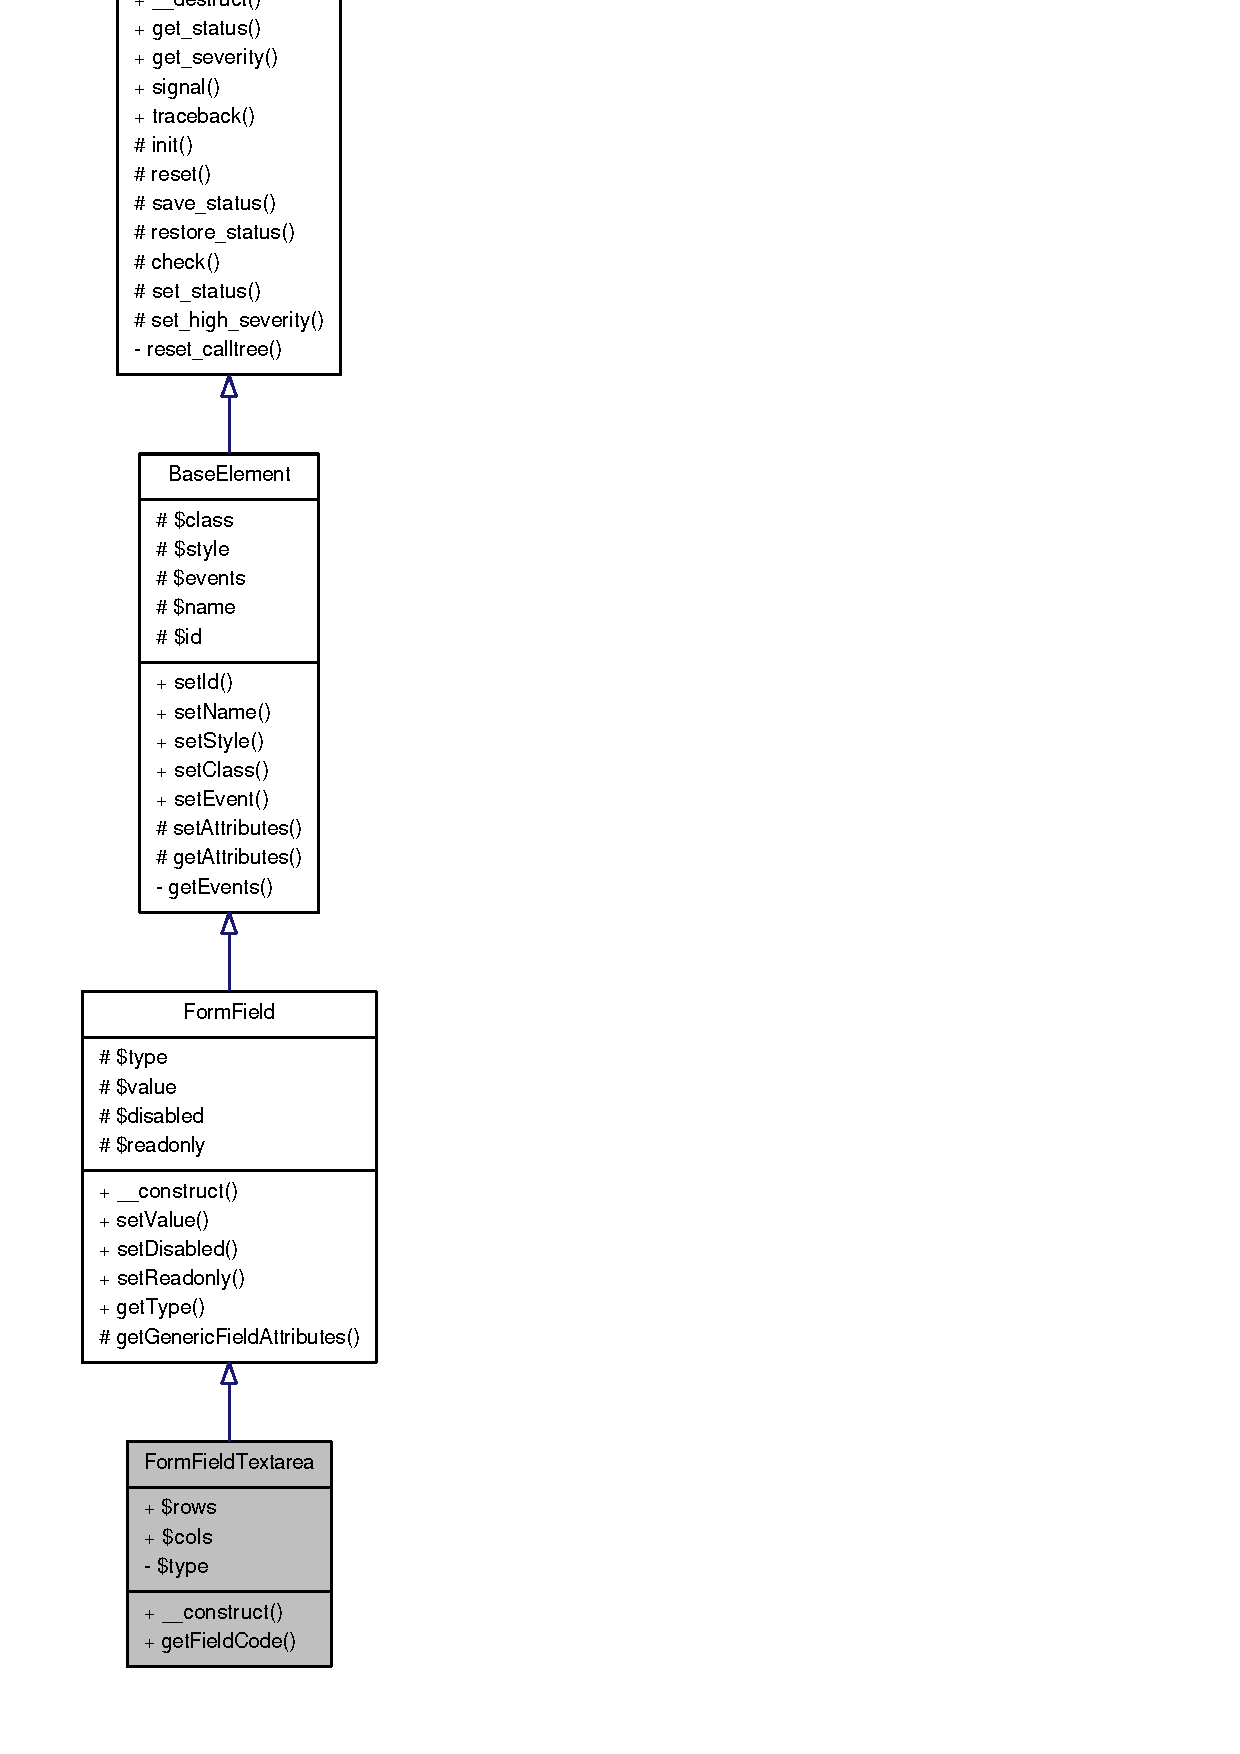
\includegraphics[height=600pt]{classFormFieldTextarea__inherit__graph}
\end{center}
\end{figure}


Collaboration diagram for FormFieldTextarea:\nopagebreak
\begin{figure}[H]
\begin{center}
\leavevmode
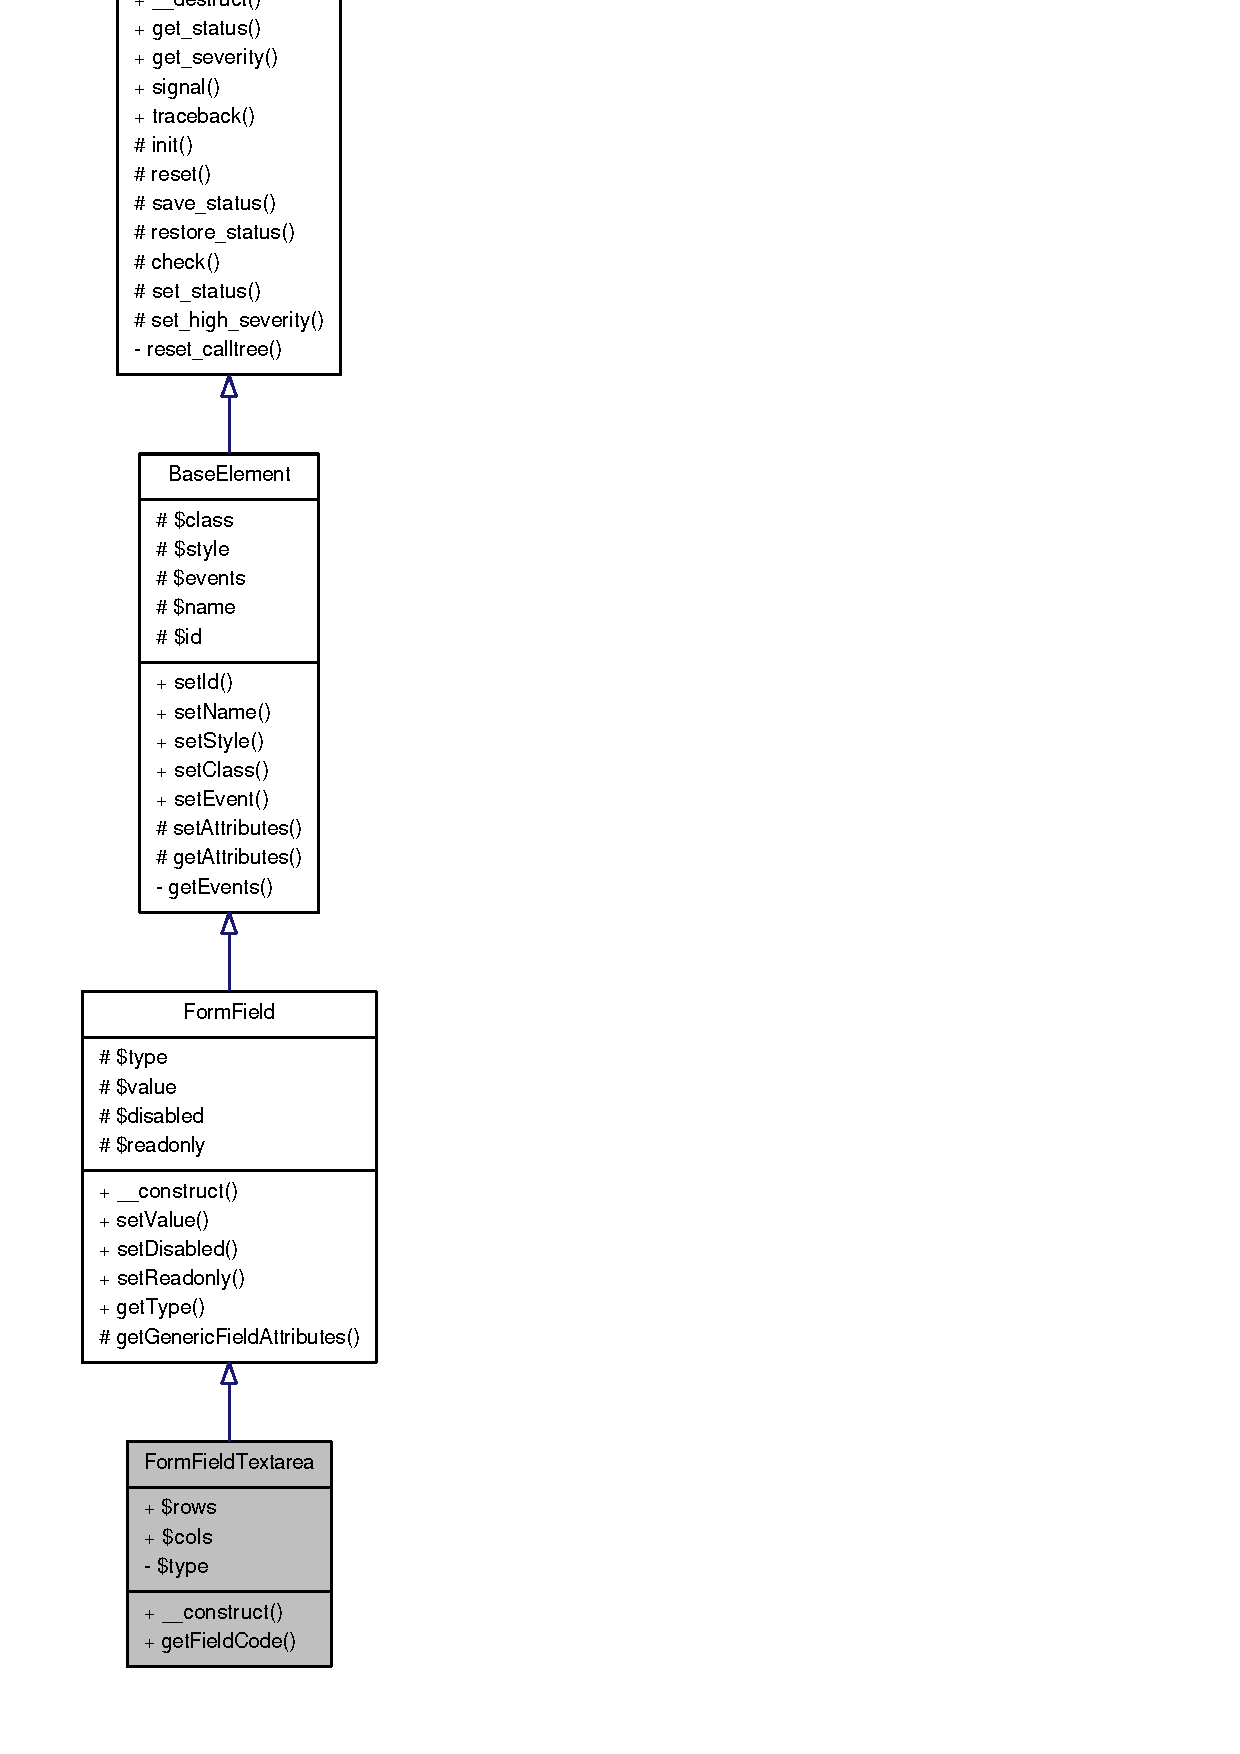
\includegraphics[height=600pt]{classFormFieldTextarea__coll__graph}
\end{center}
\end{figure}
\subsection*{Public Member Functions}
\begin{DoxyCompactItemize}
\item 
\hyperlink{classFormFieldTextarea_a65e5d308db60f1ca0d08085d09dea8bc}{\_\-\_\-construct} ()
\item 
\hyperlink{classFormFieldTextarea_aebe84c54cafbcc8b4fc32f4b5ce04f1a}{getFieldCode} ()
\item 
\hyperlink{classFormField_a465ff61e290d82be96bb793c3a14b3e7}{setValue} (\$\_\-value)
\item 
\hyperlink{classFormField_a9fa2c828eaf98154edfaa2e755657117}{setDisabled} (\$\_\-value=true)
\item 
\hyperlink{classFormField_a6eabbb35d24b1698ea25b66ddfd88a64}{setReadonly} (\$\_\-value=true)
\item 
\hyperlink{classFormField_a1f64b737bccb6b2827f8c5665b9920c7}{getType} ()
\item 
\hyperlink{classBaseElement_a0c1ce3d1684ecb78960cf7a97278494e}{setId} (\$\_\-value)
\item 
\hyperlink{classBaseElement_a39bafb3609d10048920c20242c2a04c5}{setName} (\$\_\-value)
\item 
\hyperlink{classBaseElement_a6b2b9ff69f6e92db82f91d9c55cda697}{setStyle} (\$\_\-value)
\item 
\hyperlink{classBaseElement_af6597b30fa9798878f6290271043dfa2}{setClass} (\$\_\-value)
\item 
\hyperlink{classBaseElement_ad5789f45f16aaa144716ee8558069c31}{setEvent} (\$\_\-event, \$\_\-action, \$\_\-add=false)
\item 
\hyperlink{class__OWL_a99ec771fa2c5c279f80152cc09e489a8}{get\_\-status} ()
\item 
\hyperlink{class__OWL_adf9509ef96858be7bdd9414c5ef129aa}{get\_\-severity} (\$status=null)
\item 
\hyperlink{class__OWL_a51ba4a16409acf2a2f61f286939091a5}{signal} (\$level=\hyperlink{owl_8severitycodes_8php_a139328861128689f2f4def6a399d9057}{OWL\_\-INFO}, \&\$text=false)
\item 
\hyperlink{class__OWL_aa29547995d6741b7d2b90c1d4ea99a13}{traceback} (\&\$text=false, \$depth=0)
\end{DoxyCompactItemize}
\subsection*{Public Attributes}
\begin{DoxyCompactItemize}
\item 
\hyperlink{classFormFieldTextarea_ab3a8058daa4c23d597e4003366075b59}{\$rows}
\item 
\hyperlink{classFormFieldTextarea_a70b12469646211ddd78d187269604fd4}{\$cols}
\end{DoxyCompactItemize}
\subsection*{Protected Member Functions}
\begin{DoxyCompactItemize}
\item 
\hyperlink{classFormField_a9f9d136ba8b4a793f22370aff43d592d}{getGenericFieldAttributes} (\$\_\-ignore=array())
\item 
\hyperlink{classBaseElement_aa623b042d23a5b77add8b3c452ec5855}{setAttributes} (\$\_\-attribs)
\item 
\hyperlink{classBaseElement_ae8237038633fc53db818f36da1940297}{getAttributes} (\$\_\-ignore=array())
\item 
\hyperlink{class__OWL_ae0ef3ded56e8a6b34b6461e5a721cd3e}{init} ()
\item 
\hyperlink{class__OWL_a2f2a042bcf31965194c03033df0edc9b}{reset} ()
\item 
\hyperlink{class__OWL_a9e49b9c76fbc021b244c6915ea536d71}{save\_\-status} ()
\item 
\hyperlink{class__OWL_a465eeaf40edd9f9c848841700c32ce55}{restore\_\-status} ()
\item 
\hyperlink{class__OWL_ad6f4f6946f40199dd0333cf219fa500e}{check} (\&\$object, \$level)
\item 
\hyperlink{class__OWL_aea912d0ede9b3c2a69b79072d94d4787}{set\_\-status} (\$status, \$params=array())
\item 
\hyperlink{class__OWL_a576829692a3b66e3d518853bf43abae3}{set\_\-high\_\-severity} (\&\$object=null)
\end{DoxyCompactItemize}
\subsection*{Protected Attributes}
\begin{DoxyCompactItemize}
\item 
\hyperlink{classFormField_a3c01e89834248eec8e2f145fbcfa0fbc}{\$value}
\item 
\hyperlink{classFormField_ab6f1907061890290e32cb2befc0a5f50}{\$disabled}
\item 
\hyperlink{classFormField_a78ba5d4b9127e75e8ccf86f397b5d9ac}{\$readonly}
\item 
\hyperlink{classBaseElement_a99976a8e967db92e7800309f359b0803}{\$class} = ''
\item 
\hyperlink{classBaseElement_a429a3d642dd95f30e1059ef29564b87d}{\$style} = ''
\item 
\hyperlink{classBaseElement_a02cebe45d277b4ff8f29db08bad371ba}{\$events} = array()
\item 
\hyperlink{classBaseElement_a30b8cff187a9de659a70daf287d66f45}{\$name} = ''
\item 
\hyperlink{classBaseElement_a11b6989c43b53869a09f5ce65aa55b45}{\$id} = ''
\item 
\hyperlink{class__OWL_ad26b40a9dbbacb33e299b17826f8327c}{\$severity}
\end{DoxyCompactItemize}
\subsection*{Private Attributes}
\begin{DoxyCompactItemize}
\item 
\hyperlink{classFormFieldTextarea_a85348034822c70694fc8640bfcacc04d}{\$type}
\end{DoxyCompactItemize}


\subsection{Detailed Description}
Formfield. Formfield textarea elements \begin{DoxyAuthor}{Author}
Oscar van Eijk, Oveas Functionality Provider 
\end{DoxyAuthor}
\begin{DoxyVersion}{Version}
Oct 19, 2010 -\/-\/ O van Eijk -\/-\/ initial version 
\end{DoxyVersion}


\subsection{Constructor \& Destructor Documentation}
\index{FormFieldTextarea@{FormFieldTextarea}!\_\-\_\-construct@{\_\-\_\-construct}}
\index{\_\-\_\-construct@{\_\-\_\-construct}!FormFieldTextarea@{FormFieldTextarea}}
\subsubsection[{\_\-\_\-construct}]{\setlength{\rightskip}{0pt plus 5cm}FormFieldTextarea::\_\-\_\-construct (
\begin{DoxyParamCaption}
{}
\end{DoxyParamCaption}
)}\label{classFormFieldTextarea_a65e5d308db60f1ca0d08085d09dea8bc}
Class constructor; 

Reimplemented from \hyperlink{classFormField_a0cfe713ce28a6a0cb53476ed463e1f01}{FormField}.



\subsection{Member Function Documentation}
\index{FormFieldTextarea@{FormFieldTextarea}!check@{check}}
\index{check@{check}!FormFieldTextarea@{FormFieldTextarea}}
\subsubsection[{check}]{\setlength{\rightskip}{0pt plus 5cm}\_\-OWL::check (
\begin{DoxyParamCaption}
\item[{\&\$}]{ object, }
\item[{\$}]{ level}
\end{DoxyParamCaption}
)\hspace{0.3cm}{\ttfamily  \mbox{[}protected, inherited\mbox{]}}}\label{class__OWL_ad6f4f6946f40199dd0333cf219fa500e}
This is a helper function for lazy developers. Some checks have to be made quite often, this is a kinda macro to handle that. It compares the own severity level with that of a given object. If the highest level is above a given max, a traceback and reset are performed.


\begin{DoxyParams}{Parameters}
\item[\mbox{\tt[in]} {\em \$object}]Pointer to an object to check against \item[\mbox{\tt[in]} {\em \$level}]The maximum severity level \end{DoxyParams}
\begin{DoxyReturn}{Returns}
True if the severity level was correct ( below the max), otherwise false 
\end{DoxyReturn}


References \_\-OWL::reset(), \_\-OWL::set\_\-high\_\-severity(), and \_\-OWL::traceback().



Referenced by SessionHandler::write().

\index{FormFieldTextarea@{FormFieldTextarea}!get\_\-severity@{get\_\-severity}}
\index{get\_\-severity@{get\_\-severity}!FormFieldTextarea@{FormFieldTextarea}}
\subsubsection[{get\_\-severity}]{\setlength{\rightskip}{0pt plus 5cm}\_\-OWL::get\_\-severity (
\begin{DoxyParamCaption}
\item[{\$}]{ status = {\ttfamily null}}
\end{DoxyParamCaption}
)\hspace{0.3cm}{\ttfamily  \mbox{[}inherited\mbox{]}}}\label{class__OWL_adf9509ef96858be7bdd9414c5ef129aa}
Get the current object severity level.


\begin{DoxyParams}{Parameters}
\item[\mbox{\tt[in]} {\em \$status}]An optional parameter to check an other status code i.s.o the object's current status. \end{DoxyParams}
\begin{DoxyReturn}{Returns}
Status severity level 
\end{DoxyReturn}


References \_\-OWL::\$status.



Referenced by LogHandler::compose\_\-message(), LogHandler::log(), and DataHandler::set\_\-key().

\index{FormFieldTextarea@{FormFieldTextarea}!get\_\-status@{get\_\-status}}
\index{get\_\-status@{get\_\-status}!FormFieldTextarea@{FormFieldTextarea}}
\subsubsection[{get\_\-status}]{\setlength{\rightskip}{0pt plus 5cm}\_\-OWL::get\_\-status (
\begin{DoxyParamCaption}
{}
\end{DoxyParamCaption}
)\hspace{0.3cm}{\ttfamily  \mbox{[}final, inherited\mbox{]}}}\label{class__OWL_a99ec771fa2c5c279f80152cc09e489a8}
Get the current object status.

\begin{DoxyReturn}{Returns}
Object's status code 
\end{DoxyReturn}


Referenced by SchemeHandler::compare().

\index{FormFieldTextarea@{FormFieldTextarea}!getAttributes@{getAttributes}}
\index{getAttributes@{getAttributes}!FormFieldTextarea@{FormFieldTextarea}}
\subsubsection[{getAttributes}]{\setlength{\rightskip}{0pt plus 5cm}BaseElement::getAttributes (
\begin{DoxyParamCaption}
\item[{\$}]{ \_\-ignore = {\ttfamily array()}}
\end{DoxyParamCaption}
)\hspace{0.3cm}{\ttfamily  \mbox{[}protected, inherited\mbox{]}}}\label{classBaseElement_ae8237038633fc53db818f36da1940297}
Return the general element attributes that are set 
\begin{DoxyParams}{Parameters}
\item[\mbox{\tt[in]} {\em \$\_\-ignore}]Array with attributes names that should be ignored \end{DoxyParams}
\begin{DoxyReturn}{Returns}
string attributes in HTML format (' fld=\char`\"{}value\char`\"{}...) 
\end{DoxyReturn}


References BaseElement::getEvents().



Referenced by FormField::getGenericFieldAttributes(), Table::getTable(), Tablecell::getTablecell(), Tablerow::getTablerow(), and Form::openForm().

\index{FormFieldTextarea@{FormFieldTextarea}!getFieldCode@{getFieldCode}}
\index{getFieldCode@{getFieldCode}!FormFieldTextarea@{FormFieldTextarea}}
\subsubsection[{getFieldCode}]{\setlength{\rightskip}{0pt plus 5cm}FormFieldTextarea::getFieldCode (
\begin{DoxyParamCaption}
{}
\end{DoxyParamCaption}
)}\label{classFormFieldTextarea_aebe84c54cafbcc8b4fc32f4b5ce04f1a}
Return the HTML code to display the form element

\begin{DoxyReturn}{Returns}
Textstring with the complete code for the form element 
\end{DoxyReturn}


References FormField::getGenericFieldAttributes().

\index{FormFieldTextarea@{FormFieldTextarea}!getGenericFieldAttributes@{getGenericFieldAttributes}}
\index{getGenericFieldAttributes@{getGenericFieldAttributes}!FormFieldTextarea@{FormFieldTextarea}}
\subsubsection[{getGenericFieldAttributes}]{\setlength{\rightskip}{0pt plus 5cm}FormField::getGenericFieldAttributes (
\begin{DoxyParamCaption}
\item[{\$}]{ \_\-ignore = {\ttfamily array()}}
\end{DoxyParamCaption}
)\hspace{0.3cm}{\ttfamily  \mbox{[}protected, inherited\mbox{]}}}\label{classFormField_a9f9d136ba8b4a793f22370aff43d592d}
Return the attributes for an HTML formfield in the \char`\"{} attrib='value' \mbox{[}...\mbox{]}\char`\"{} format


\begin{DoxyParams}{Parameters}
\item[\mbox{\tt[in]} {\em \$\_\-ignore}]Array with attributes names that should be ignored, e.g. for a textarea, the value is not returned as an attribute. \end{DoxyParams}
\begin{DoxyReturn}{Returns}
Textstring with the HTML code 
\end{DoxyReturn}


References BaseElement::getAttributes().



Referenced by getFieldCode(), FormFieldText::getFieldCode(), FormFieldSelect::getFieldCode(), FormFieldRadio::getFieldCode(), FormFieldCheckbox::getFieldCode(), and FormFieldButton::getFieldCode().

\index{FormFieldTextarea@{FormFieldTextarea}!getType@{getType}}
\index{getType@{getType}!FormFieldTextarea@{FormFieldTextarea}}
\subsubsection[{getType}]{\setlength{\rightskip}{0pt plus 5cm}FormField::getType (
\begin{DoxyParamCaption}
{}
\end{DoxyParamCaption}
)\hspace{0.3cm}{\ttfamily  \mbox{[}inherited\mbox{]}}}\label{classFormField_a1f64b737bccb6b2827f8c5665b9920c7}
Give the field type \begin{DoxyReturn}{Returns}
Field type 
\end{DoxyReturn}
\index{FormFieldTextarea@{FormFieldTextarea}!init@{init}}
\index{init@{init}!FormFieldTextarea@{FormFieldTextarea}}
\subsubsection[{init}]{\setlength{\rightskip}{0pt plus 5cm}\_\-OWL::init (
\begin{DoxyParamCaption}
{}
\end{DoxyParamCaption}
)\hspace{0.3cm}{\ttfamily  \mbox{[}protected, inherited\mbox{]}}}\label{class__OWL_ae0ef3ded56e8a6b34b6461e5a721cd3e}
This function should be called by all constuctors. It initializes the general characteristics. Status is 'warning' by default, it's up to the contructor to set a proper status; if it's still 'warning', this $\ast$might$\ast$ indicate something went wrong. 

References OWL::factory().



Referenced by Tablerow::\_\-\_\-construct(), Tablecell::\_\-\_\-construct(), Table::\_\-\_\-construct(), FormField::\_\-\_\-construct(), UserHandler::\_\-\_\-construct(), SessionHandler::\_\-\_\-construct(), SchemeHandler::\_\-\_\-construct(), LogHandler::\_\-\_\-construct(), ImageHandler::\_\-\_\-construct(), FormHandler::\_\-\_\-construct(), FileHandler::\_\-\_\-construct(), DbHandler::\_\-\_\-construct(), OWL::\_\-\_\-construct(), Form::\_\-\_\-construct(), Dispatcher::\_\-\_\-construct(), and DataHandler::DataHandler().

\index{FormFieldTextarea@{FormFieldTextarea}!reset@{reset}}
\index{reset@{reset}!FormFieldTextarea@{FormFieldTextarea}}
\subsubsection[{reset}]{\setlength{\rightskip}{0pt plus 5cm}\_\-OWL::reset (
\begin{DoxyParamCaption}
{}
\end{DoxyParamCaption}
)\hspace{0.3cm}{\ttfamily  \mbox{[}protected, inherited\mbox{]}}}\label{class__OWL_a2f2a042bcf31965194c03033df0edc9b}
General reset function for all objects. Should be called after each non-\/fatal error 

Reimplemented in \hyperlink{classDbHandler_a9982df4830f05803935bb31bac7fae3d}{DbHandler}, and \hyperlink{classSchemeHandler_aa25feb4a70d67b3d571904be4b2f50bc}{SchemeHandler}.



References \_\-OWL::reset\_\-calltree().



Referenced by \_\-OWL::check(), SessionHandler::read(), DataHandler::reset(), and \_\-OWL::set\_\-status().

\index{FormFieldTextarea@{FormFieldTextarea}!restore\_\-status@{restore\_\-status}}
\index{restore\_\-status@{restore\_\-status}!FormFieldTextarea@{FormFieldTextarea}}
\subsubsection[{restore\_\-status}]{\setlength{\rightskip}{0pt plus 5cm}\_\-OWL::restore\_\-status (
\begin{DoxyParamCaption}
{}
\end{DoxyParamCaption}
)\hspace{0.3cm}{\ttfamily  \mbox{[}protected, inherited\mbox{]}}}\label{class__OWL_a465eeaf40edd9f9c848841700c32ce55}
Restore the previously saved status object and destroy the copy 

References \_\-OWL::set\_\-status().



Referenced by UserHandler::logout().

\index{FormFieldTextarea@{FormFieldTextarea}!save\_\-status@{save\_\-status}}
\index{save\_\-status@{save\_\-status}!FormFieldTextarea@{FormFieldTextarea}}
\subsubsection[{save\_\-status}]{\setlength{\rightskip}{0pt plus 5cm}\_\-OWL::save\_\-status (
\begin{DoxyParamCaption}
{}
\end{DoxyParamCaption}
)\hspace{0.3cm}{\ttfamily  \mbox{[}protected, inherited\mbox{]}}}\label{class__OWL_a9e49b9c76fbc021b244c6915ea536d71}
Create a copy of the status object 

Referenced by UserHandler::logout().

\index{FormFieldTextarea@{FormFieldTextarea}!set\_\-high\_\-severity@{set\_\-high\_\-severity}}
\index{set\_\-high\_\-severity@{set\_\-high\_\-severity}!FormFieldTextarea@{FormFieldTextarea}}
\subsubsection[{set\_\-high\_\-severity}]{\setlength{\rightskip}{0pt plus 5cm}\_\-OWL::set\_\-high\_\-severity (
\begin{DoxyParamCaption}
\item[{\&\$}]{ object = {\ttfamily null}}
\end{DoxyParamCaption}
)\hspace{0.3cm}{\ttfamily  \mbox{[}protected, inherited\mbox{]}}}\label{class__OWL_a576829692a3b66e3d518853bf43abae3}
Compare the severity level of the current object with a given one and set my statuspointer to the object with the highest level. 

Referenced by \_\-OWL::check(), DataHandler::db(), DataHandler::prepare(), and SessionHandler::read().

\index{FormFieldTextarea@{FormFieldTextarea}!set\_\-status@{set\_\-status}}
\index{set\_\-status@{set\_\-status}!FormFieldTextarea@{FormFieldTextarea}}
\subsubsection[{set\_\-status}]{\setlength{\rightskip}{0pt plus 5cm}\_\-OWL::set\_\-status (
\begin{DoxyParamCaption}
\item[{\$}]{ status, }
\item[{\$}]{ params = {\ttfamily array~()}}
\end{DoxyParamCaption}
)\hspace{0.3cm}{\ttfamily  \mbox{[}final, protected, inherited\mbox{]}}}\label{class__OWL_aea912d0ede9b3c2a69b79072d94d4787}
Set the current object status to the specified value.


\begin{DoxyParams}{Parameters}
\item[\mbox{\tt[in]} {\em \$status}]\hyperlink{classOWL}{OWL} status code \item[\mbox{\tt[in]} {\em \$params}]\end{DoxyParams}


References \$GLOBALS, \_\-OWL::\$status, ConfigHandler::get(), Register::get\_\-code(), \_\-OWL::reset(), and \_\-OWL::signal().



Referenced by UserHandler::\_\-\_\-construct(), SessionHandler::\_\-\_\-construct(), SchemeHandler::\_\-\_\-construct(), ImageHandler::\_\-\_\-construct(), FormHandler::\_\-\_\-construct(), FileHandler::\_\-\_\-construct(), DbHandler::\_\-\_\-construct(), Form::\_\-\_\-construct(), Form::addField(), SchemeHandler::alter\_\-scheme(), FileHandler::close(), DbHandler::connect(), DbHandler::create(), SchemeHandler::create\_\-scheme(), DataHandler::DataHandler(), SchemeHandler::define\_\-index(), SchemeHandler::define\_\-scheme(), Dispatcher::dispatch(), FormHandler::get(), DataHandler::get(), SchemeHandler::get\_\-table\_\-columns(), SchemeHandler::get\_\-table\_\-indexes(), UserHandler::login(), FileHandler::open(), DbHandler::open(), LogHandler::open\_\-logfile(), DataHandler::prepare(), DbHandler::prepare\_\-delete(), DbHandler::prepare\_\-insert(), DbHandler::prepare\_\-read(), DbHandler::prepare\_\-update(), DbHandler::read(), FileHandler::read\_\-line(), UserHandler::read\_\-userdata(), \_\-OWL::restore\_\-status(), SchemeHandler::scheme(), FormHandler::set(), DataHandler::set(), DataHandler::set\_\-join(), DataHandler::set\_\-key(), BaseElement::setAttributes(), Form::setEncoding(), Form::setFieldAttributes(), FormFieldText::setMaxsize(), Form::setMethod(), FormFieldRadio::setSelected(), FormFieldText::setSize(), FormFieldSelect::setSize(), FormFieldSelect::setValue(), FormFieldRadio::setValue(), Form::showField(), SchemeHandler::table\_\-description(), SchemeHandler::validate\_\-scheme(), and DbHandler::write().

\index{FormFieldTextarea@{FormFieldTextarea}!setAttributes@{setAttributes}}
\index{setAttributes@{setAttributes}!FormFieldTextarea@{FormFieldTextarea}}
\subsubsection[{setAttributes}]{\setlength{\rightskip}{0pt plus 5cm}BaseElement::setAttributes (
\begin{DoxyParamCaption}
\item[{\$}]{ \_\-attribs}
\end{DoxyParamCaption}
)\hspace{0.3cm}{\ttfamily  \mbox{[}protected, inherited\mbox{]}}}\label{classBaseElement_aa623b042d23a5b77add8b3c452ec5855}
Set the attributes of the DOM element by calling the 'set$<$Attrib$>$' method for this class. 
\begin{DoxyParams}{Parameters}
\item[\mbox{\tt[in]} {\em \$\_\-attribs}]Array with attributes in the format attrib=$>$value \end{DoxyParams}
\begin{DoxyReturn}{Returns}
Severity level. The status increased when a set$<$Attrib\&gt method does not exist. 
\end{DoxyReturn}


Reimplemented in \hyperlink{classTablecell_a91a8264df222cc44b77ceaf7282a400e}{Tablecell}, and \hyperlink{classTablerow_aece4cad0834c299d7e03030e945aea3a}{Tablerow}.



References \_\-OWL::set\_\-status().



Referenced by Table::\_\-\_\-construct().

\index{FormFieldTextarea@{FormFieldTextarea}!setClass@{setClass}}
\index{setClass@{setClass}!FormFieldTextarea@{FormFieldTextarea}}
\subsubsection[{setClass}]{\setlength{\rightskip}{0pt plus 5cm}BaseElement::setClass (
\begin{DoxyParamCaption}
\item[{\$}]{ \_\-value}
\end{DoxyParamCaption}
)\hspace{0.3cm}{\ttfamily  \mbox{[}inherited\mbox{]}}}\label{classBaseElement_af6597b30fa9798878f6290271043dfa2}
Set the element Class 
\begin{DoxyParams}{Parameters}
\item[\mbox{\tt[in]} {\em \$\_\-value}]Class name \end{DoxyParams}
\index{FormFieldTextarea@{FormFieldTextarea}!setDisabled@{setDisabled}}
\index{setDisabled@{setDisabled}!FormFieldTextarea@{FormFieldTextarea}}
\subsubsection[{setDisabled}]{\setlength{\rightskip}{0pt plus 5cm}FormField::setDisabled (
\begin{DoxyParamCaption}
\item[{\$}]{ \_\-value = {\ttfamily true}}
\end{DoxyParamCaption}
)\hspace{0.3cm}{\ttfamily  \mbox{[}inherited\mbox{]}}}\label{classFormField_a9fa2c828eaf98154edfaa2e755657117}
Set the Disabled boolean 
\begin{DoxyParams}{Parameters}
\item[\mbox{\tt[in]} {\em \$\_\-value}]Value indicating true (default) or false \end{DoxyParams}
\index{FormFieldTextarea@{FormFieldTextarea}!setEvent@{setEvent}}
\index{setEvent@{setEvent}!FormFieldTextarea@{FormFieldTextarea}}
\subsubsection[{setEvent}]{\setlength{\rightskip}{0pt plus 5cm}BaseElement::setEvent (
\begin{DoxyParamCaption}
\item[{\$}]{ \_\-event, }
\item[{\$}]{ \_\-action, }
\item[{\$}]{ \_\-add = {\ttfamily false}}
\end{DoxyParamCaption}
)\hspace{0.3cm}{\ttfamily  \mbox{[}inherited\mbox{]}}}\label{classBaseElement_ad5789f45f16aaa144716ee8558069c31}
Add an event to the events array 
\begin{DoxyParams}{Parameters}
\item[\mbox{\tt[in]} {\em \$\_\-event}]Javascript event name (onXxx) \item[\mbox{\tt[in]} {\em \$\_\-action}]Javascript function or code \item[\mbox{\tt[in]} {\em \$\_\-add}]Boolean; when true, the action will be added if the event name already exists. Default is false; overwrite the action for this event. \end{DoxyParams}
\index{FormFieldTextarea@{FormFieldTextarea}!setId@{setId}}
\index{setId@{setId}!FormFieldTextarea@{FormFieldTextarea}}
\subsubsection[{setId}]{\setlength{\rightskip}{0pt plus 5cm}BaseElement::setId (
\begin{DoxyParamCaption}
\item[{\$}]{ \_\-value}
\end{DoxyParamCaption}
)\hspace{0.3cm}{\ttfamily  \mbox{[}inherited\mbox{]}}}\label{classBaseElement_a0c1ce3d1684ecb78960cf7a97278494e}
Set the element ID 
\begin{DoxyParams}{Parameters}
\item[\mbox{\tt[in]} {\em \$\_\-value}]Identification \end{DoxyParams}
\index{FormFieldTextarea@{FormFieldTextarea}!setName@{setName}}
\index{setName@{setName}!FormFieldTextarea@{FormFieldTextarea}}
\subsubsection[{setName}]{\setlength{\rightskip}{0pt plus 5cm}BaseElement::setName (
\begin{DoxyParamCaption}
\item[{\$}]{ \_\-value}
\end{DoxyParamCaption}
)\hspace{0.3cm}{\ttfamily  \mbox{[}inherited\mbox{]}}}\label{classBaseElement_a39bafb3609d10048920c20242c2a04c5}
Set the element name 
\begin{DoxyParams}{Parameters}
\item[\mbox{\tt[in]} {\em \$\_\-value}]Element name \end{DoxyParams}
\index{FormFieldTextarea@{FormFieldTextarea}!setReadonly@{setReadonly}}
\index{setReadonly@{setReadonly}!FormFieldTextarea@{FormFieldTextarea}}
\subsubsection[{setReadonly}]{\setlength{\rightskip}{0pt plus 5cm}FormField::setReadonly (
\begin{DoxyParamCaption}
\item[{\$}]{ \_\-value = {\ttfamily true}}
\end{DoxyParamCaption}
)\hspace{0.3cm}{\ttfamily  \mbox{[}inherited\mbox{]}}}\label{classFormField_a6eabbb35d24b1698ea25b66ddfd88a64}
Set the Readonly boolean 
\begin{DoxyParams}{Parameters}
\item[\mbox{\tt[in]} {\em \$\_\-value}]Value indicating true (default) or false \end{DoxyParams}
\index{FormFieldTextarea@{FormFieldTextarea}!setStyle@{setStyle}}
\index{setStyle@{setStyle}!FormFieldTextarea@{FormFieldTextarea}}
\subsubsection[{setStyle}]{\setlength{\rightskip}{0pt plus 5cm}BaseElement::setStyle (
\begin{DoxyParamCaption}
\item[{\$}]{ \_\-value}
\end{DoxyParamCaption}
)\hspace{0.3cm}{\ttfamily  \mbox{[}inherited\mbox{]}}}\label{classBaseElement_a6b2b9ff69f6e92db82f91d9c55cda697}
Set the element style 
\begin{DoxyParams}{Parameters}
\item[\mbox{\tt[in]} {\em \$\_\-value}]Element style \end{DoxyParams}
\index{FormFieldTextarea@{FormFieldTextarea}!setValue@{setValue}}
\index{setValue@{setValue}!FormFieldTextarea@{FormFieldTextarea}}
\subsubsection[{setValue}]{\setlength{\rightskip}{0pt plus 5cm}FormField::setValue (
\begin{DoxyParamCaption}
\item[{\$}]{ \_\-value}
\end{DoxyParamCaption}
)\hspace{0.3cm}{\ttfamily  \mbox{[}inherited\mbox{]}}}\label{classFormField_a465ff61e290d82be96bb793c3a14b3e7}
Set the field value 
\begin{DoxyParams}{Parameters}
\item[\mbox{\tt[in]} {\em \$\_\-value}]Field value \end{DoxyParams}


Reimplemented in \hyperlink{classFormFieldCheckbox_a787abee157599c389a18e0810f69fed5}{FormFieldCheckbox}, \hyperlink{classFormFieldRadio_aab105e92866fd80890d3254f51a2e4ca}{FormFieldRadio}, and \hyperlink{classFormFieldSelect_ae69f5b352df63796c048dca6a2de7544}{FormFieldSelect}.

\index{FormFieldTextarea@{FormFieldTextarea}!signal@{signal}}
\index{signal@{signal}!FormFieldTextarea@{FormFieldTextarea}}
\subsubsection[{signal}]{\setlength{\rightskip}{0pt plus 5cm}\_\-OWL::signal (
\begin{DoxyParamCaption}
\item[{\$}]{ level = {\ttfamily {\bf OWL\_\-INFO}}, }
\item[{\&\$}]{ text = {\ttfamily false}}
\end{DoxyParamCaption}
)\hspace{0.3cm}{\ttfamily  \mbox{[}inherited\mbox{]}}}\label{class__OWL_a51ba4a16409acf2a2f61f286939091a5}
Display the message for the current object status


\begin{DoxyParams}{Parameters}
\item[\mbox{\tt[in]} {\em \$level}]An optional severity level; message will only be displayed when it is at least of this level. \item[\mbox{\tt[out]} {\em \$text}]If this parameter is given, the message text is returned in this string instead of echood. \end{DoxyParams}
\begin{DoxyReturn}{Returns}
The severity level for this object 
\end{DoxyReturn}


References ConfigHandler::get().



Referenced by \_\-OWL::set\_\-status(), and \_\-OWL::traceback().

\index{FormFieldTextarea@{FormFieldTextarea}!traceback@{traceback}}
\index{traceback@{traceback}!FormFieldTextarea@{FormFieldTextarea}}
\subsubsection[{traceback}]{\setlength{\rightskip}{0pt plus 5cm}\_\-OWL::traceback (
\begin{DoxyParamCaption}
\item[{\&\$}]{ text = {\ttfamily false}, }
\item[{\$}]{ depth = {\ttfamily 0}}
\end{DoxyParamCaption}
)\hspace{0.3cm}{\ttfamily  \mbox{[}inherited\mbox{]}}}\label{class__OWL_aa29547995d6741b7d2b90c1d4ea99a13}
If somehwere in the nested calls an error occured, we can traceback the original failing object with this function and signal the message.


\begin{DoxyParams}{Parameters}
\item[\mbox{\tt[out]} {\em \$text}]Optional variable in which the message text can be stored. If not given, the text will be written to standard output \item[\mbox{\tt[in]} {\em \$depth}]This paramater should be initially empty. It calculates the depth in recursive calls. \end{DoxyParams}
\begin{DoxyReturn}{Returns}
Severity code of the failing object 
\end{DoxyReturn}


References \_\-OWL::signal().



Referenced by \_\-OWL::check(), UserHandler::login(), and SessionHandler::read().



\subsection{Member Data Documentation}
\index{FormFieldTextarea@{FormFieldTextarea}!\$class@{\$class}}
\index{\$class@{\$class}!FormFieldTextarea@{FormFieldTextarea}}
\subsubsection[{\$class}]{\setlength{\rightskip}{0pt plus 5cm}BaseElement::\$class = ''\hspace{0.3cm}{\ttfamily  \mbox{[}protected, inherited\mbox{]}}}\label{classBaseElement_a99976a8e967db92e7800309f359b0803}
Class specification \index{FormFieldTextarea@{FormFieldTextarea}!\$cols@{\$cols}}
\index{\$cols@{\$cols}!FormFieldTextarea@{FormFieldTextarea}}
\subsubsection[{\$cols}]{\setlength{\rightskip}{0pt plus 5cm}FormFieldTextarea::\$cols}\label{classFormFieldTextarea_a70b12469646211ddd78d187269604fd4}
Number of rows in the textarea \index{FormFieldTextarea@{FormFieldTextarea}!\$disabled@{\$disabled}}
\index{\$disabled@{\$disabled}!FormFieldTextarea@{FormFieldTextarea}}
\subsubsection[{\$disabled}]{\setlength{\rightskip}{0pt plus 5cm}FormField::\$disabled\hspace{0.3cm}{\ttfamily  \mbox{[}protected, inherited\mbox{]}}}\label{classFormField_ab6f1907061890290e32cb2befc0a5f50}
Boolean indicating a disabled field when true \index{FormFieldTextarea@{FormFieldTextarea}!\$events@{\$events}}
\index{\$events@{\$events}!FormFieldTextarea@{FormFieldTextarea}}
\subsubsection[{\$events}]{\setlength{\rightskip}{0pt plus 5cm}BaseElement::\$events = array()\hspace{0.3cm}{\ttfamily  \mbox{[}protected, inherited\mbox{]}}}\label{classBaseElement_a02cebe45d277b4ff8f29db08bad371ba}
Array with javascript events 

Referenced by Form::setFieldEvents().

\index{FormFieldTextarea@{FormFieldTextarea}!\$id@{\$id}}
\index{\$id@{\$id}!FormFieldTextarea@{FormFieldTextarea}}
\subsubsection[{\$id}]{\setlength{\rightskip}{0pt plus 5cm}BaseElement::\$id = ''\hspace{0.3cm}{\ttfamily  \mbox{[}protected, inherited\mbox{]}}}\label{classBaseElement_a11b6989c43b53869a09f5ce65aa55b45}
Element ID \index{FormFieldTextarea@{FormFieldTextarea}!\$name@{\$name}}
\index{\$name@{\$name}!FormFieldTextarea@{FormFieldTextarea}}
\subsubsection[{\$name}]{\setlength{\rightskip}{0pt plus 5cm}BaseElement::\$name = ''\hspace{0.3cm}{\ttfamily  \mbox{[}protected, inherited\mbox{]}}}\label{classBaseElement_a30b8cff187a9de659a70daf287d66f45}
Name of the element 

Referenced by Form::addField(), and Form::showField().

\index{FormFieldTextarea@{FormFieldTextarea}!\$readonly@{\$readonly}}
\index{\$readonly@{\$readonly}!FormFieldTextarea@{FormFieldTextarea}}
\subsubsection[{\$readonly}]{\setlength{\rightskip}{0pt plus 5cm}FormField::\$readonly\hspace{0.3cm}{\ttfamily  \mbox{[}protected, inherited\mbox{]}}}\label{classFormField_a78ba5d4b9127e75e8ccf86f397b5d9ac}
Boolean indicating a readonly field when true \index{FormFieldTextarea@{FormFieldTextarea}!\$rows@{\$rows}}
\index{\$rows@{\$rows}!FormFieldTextarea@{FormFieldTextarea}}
\subsubsection[{\$rows}]{\setlength{\rightskip}{0pt plus 5cm}FormFieldTextarea::\$rows}\label{classFormFieldTextarea_ab3a8058daa4c23d597e4003366075b59}
Number of columns in the textarea \index{FormFieldTextarea@{FormFieldTextarea}!\$severity@{\$severity}}
\index{\$severity@{\$severity}!FormFieldTextarea@{FormFieldTextarea}}
\subsubsection[{\$severity}]{\setlength{\rightskip}{0pt plus 5cm}\_\-OWL::\$severity\hspace{0.3cm}{\ttfamily  \mbox{[}protected, inherited\mbox{]}}}\label{class__OWL_ad26b40a9dbbacb33e299b17826f8327c}
Severity level of the current object status \index{FormFieldTextarea@{FormFieldTextarea}!\$style@{\$style}}
\index{\$style@{\$style}!FormFieldTextarea@{FormFieldTextarea}}
\subsubsection[{\$style}]{\setlength{\rightskip}{0pt plus 5cm}BaseElement::\$style = ''\hspace{0.3cm}{\ttfamily  \mbox{[}protected, inherited\mbox{]}}}\label{classBaseElement_a429a3d642dd95f30e1059ef29564b87d}
Element style \index{FormFieldTextarea@{FormFieldTextarea}!\$type@{\$type}}
\index{\$type@{\$type}!FormFieldTextarea@{FormFieldTextarea}}
\subsubsection[{\$type}]{\setlength{\rightskip}{0pt plus 5cm}FormFieldTextarea::\$type\hspace{0.3cm}{\ttfamily  \mbox{[}private\mbox{]}}}\label{classFormFieldTextarea_a85348034822c70694fc8640bfcacc04d}
Field type; this class is used for 'text' and 'password' types 

Reimplemented from \hyperlink{classFormField_a37bed21a1891e95be0e4a697e45ba51b}{FormField}.

\index{FormFieldTextarea@{FormFieldTextarea}!\$value@{\$value}}
\index{\$value@{\$value}!FormFieldTextarea@{FormFieldTextarea}}
\subsubsection[{\$value}]{\setlength{\rightskip}{0pt plus 5cm}FormField::\$value\hspace{0.3cm}{\ttfamily  \mbox{[}protected, inherited\mbox{]}}}\label{classFormField_a3c01e89834248eec8e2f145fbcfa0fbc}
Field value 

The documentation for this class was generated from the following file:\begin{DoxyCompactItemize}
\item 
/home/oscar/projects/owl-\/php/src/kernel/ui/formfields/\hyperlink{class_8formfield_8textarea_8php}{class.formfield.textarea.php}\end{DoxyCompactItemize}

\section{FormHandler Class Reference}
\label{classFormHandler}\index{FormHandler@{FormHandler}}


Formhandler.  


Inheritance diagram for FormHandler:\begin{figure}[H]
\begin{center}
\leavevmode
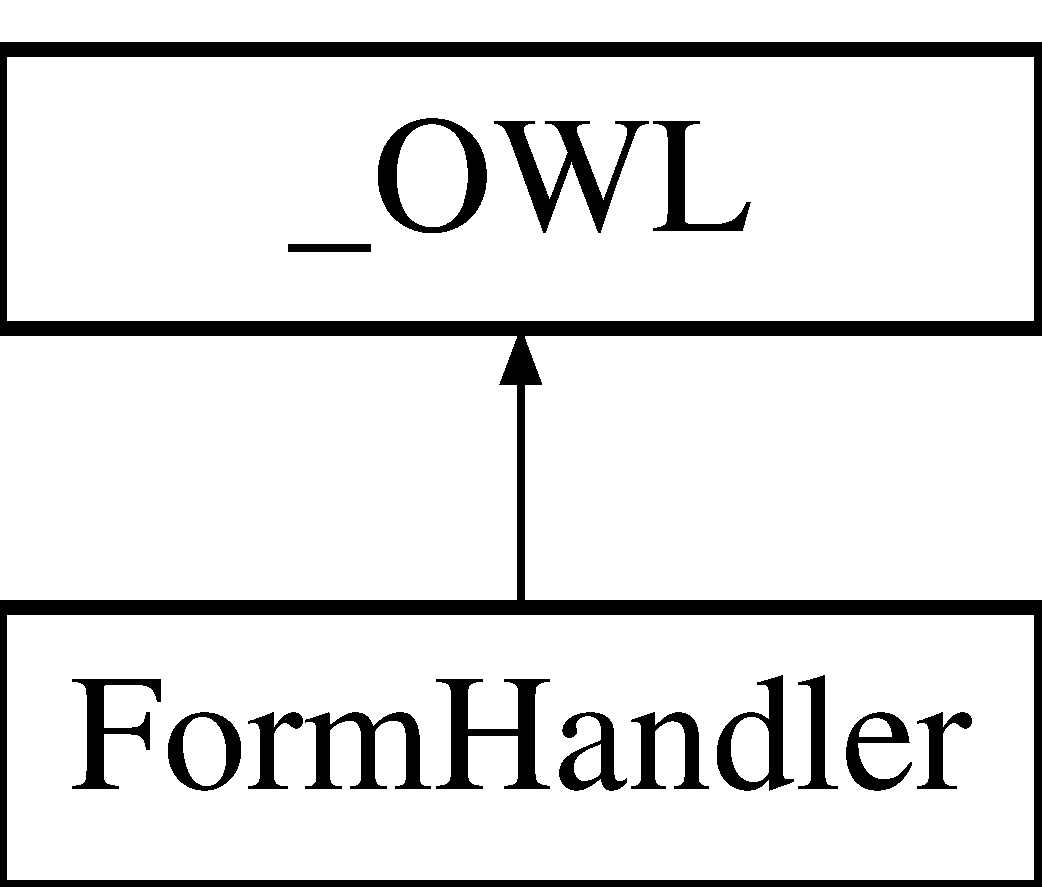
\includegraphics[height=2.000000cm]{classFormHandler}
\end{center}
\end{figure}
\subsection*{Public Member Functions}
\begin{DoxyCompactItemize}
\item 
{\bf set} (\$variable, \$value)
\item 
{\bf get} (\$variable, \$format={\bf FORMDATA\_\-STRICT}, \$allows=null, \$content=array('script'))
\item 
{\bf cleanString} (\$input, \$allow=null, \$content=null, \$remove\_\-comment=true)
\item 
{\bf get\_\-form\_\-data} ()
\item 
{\bf get\_\-status} ()
\item 
{\bf get\_\-severity} (\$status=null)
\item 
{\bf succeeded} (\$\_\-ok={\bf OWL\_\-SUCCESS}, \&\$\_\-object=null)
\item 
{\bf signal} (\$level={\bf OWL\_\-INFO}, \&\$text=false)
\item 
{\bf traceback} (\&\$text=false, \$depth=0)
\end{DoxyCompactItemize}
\subsection*{Static Public Member Functions}
\begin{DoxyCompactItemize}
\item 
static {\bf get\_\-instance} ()
\end{DoxyCompactItemize}
\subsection*{Protected Member Functions}
\begin{DoxyCompactItemize}
\item 
{\bf init} ()
\item 
{\bf set\_\-callback} (\$\_\-dispatcher)
\item 
{\bf set\_\-callback\_\-argument} (array \$\_\-arg)
\item 
{\bf get\_\-callback} ()
\item 
{\bf reset} ()
\item 
{\bf save\_\-status} ()
\item 
{\bf restore\_\-status} ()
\item 
{\bf check} (\&\$object, \$level={\bf OWL\_\-WARNING})
\item 
{\bf set\_\-status} (\$status, \$params=array())
\item 
{\bf set\_\-high\_\-severity} (\&\$object=null)
\end{DoxyCompactItemize}
\subsection*{Protected Attributes}
\begin{DoxyCompactItemize}
\item 
{\bf \$severity}
\end{DoxyCompactItemize}
\subsection*{Private Member Functions}
\begin{DoxyCompactItemize}
\item 
{\bf \_\-\_\-construct} ()
\item 
{\bf parse\_\-formdata} (\$data=null)
\end{DoxyCompactItemize}
\subsection*{Private Attributes}
\begin{DoxyCompactItemize}
\item 
{\bf \$owl\_\-formvalues}
\end{DoxyCompactItemize}
\subsection*{Static Private Attributes}
\begin{DoxyCompactItemize}
\item 
static {\bf \$instance}
\end{DoxyCompactItemize}


\subsection{Detailed Description}
Formhandler. 

Handler for all incoming formdata. \begin{DoxyAuthor}{Author}
Oscar van Eijk, Oveas Functionality Provider 
\end{DoxyAuthor}
\begin{DoxyVersion}{Version}
Aug 28, 2008 -\/-\/ O van Eijk -\/-\/ initial version 
\end{DoxyVersion}


\subsection{Constructor \& Destructor Documentation}
\index{FormHandler@{FormHandler}!\_\-\_\-construct@{\_\-\_\-construct}}
\index{\_\-\_\-construct@{\_\-\_\-construct}!FormHandler@{FormHandler}}
\subsubsection[{\_\-\_\-construct}]{\setlength{\rightskip}{0pt plus 5cm}FormHandler::\_\-\_\-construct (
\begin{DoxyParamCaption}
{}
\end{DoxyParamCaption}
)\hspace{0.3cm}{\ttfamily  [private]}}\label{classFormHandler_a1ef7ad4fe143dd8339c8ab66423a1934}
Class constructor; Parse the incoming formdata. 

References \_\-OWL::init(), parse\_\-formdata(), and \_\-OWL::set\_\-status().



\subsection{Member Function Documentation}
\index{FormHandler@{FormHandler}!check@{check}}
\index{check@{check}!FormHandler@{FormHandler}}
\subsubsection[{check}]{\setlength{\rightskip}{0pt plus 5cm}\_\-OWL::check (
\begin{DoxyParamCaption}
\item[{\&\$}]{object, }
\item[{\$}]{level = {\ttfamily {\bf OWL\_\-WARNING}}}
\end{DoxyParamCaption}
)\hspace{0.3cm}{\ttfamily  [protected, inherited]}}\label{class__OWL_ae2e3c56e5f3c4ce4156c6b1bb1c50f63}
This is a helper function for lazy developers. Some checks have to be made quite often, this is a kinda macro to handle that. It compares the own severity level with that of a given object. If the highest level is above a given max, a traceback and reset are performed.


\begin{DoxyParams}[1]{Parameters}
\mbox{\tt in}  & {\em \$object} & Pointer to an object to check against \\
\hline
\mbox{\tt in}  & {\em \$level} & The maximum severity level \\
\hline
\end{DoxyParams}
\begin{DoxyReturn}{Returns}
True if the severity level was correct (below the max), otherwise false 
\end{DoxyReturn}


References \_\-OWL::reset(), \_\-OWL::set\_\-high\_\-severity(), and \_\-OWL::traceback().



Referenced by SessionHandler::write().

\index{FormHandler@{FormHandler}!cleanString@{cleanString}}
\index{cleanString@{cleanString}!FormHandler@{FormHandler}}
\subsubsection[{cleanString}]{\setlength{\rightskip}{0pt plus 5cm}FormHandler::cleanString (
\begin{DoxyParamCaption}
\item[{\$}]{input, }
\item[{\$}]{allow = {\ttfamily null}, }
\item[{\$}]{content = {\ttfamily null}, }
\item[{\$}]{remove\_\-comment = {\ttfamily true}}
\end{DoxyParamCaption}
)}\label{classFormHandler_a5ee0cda14dcbe0b6e12226db4bd951a0}
Remove all tags from an input string 
\begin{DoxyParams}[1]{Parameters}
\mbox{\tt in}  & {\em \$input} & Input string to clean \\
\hline
\mbox{\tt in}  & {\em \$allow} & array with tags that should not be removed. These can be in a regular expression format, e.g. array('b', 'h[1-\/6]') to allow the $<$b$>$ tag and $<$h1$>$ to $<$h6$>$. \\
\hline
\mbox{\tt in}  & {\em \$content} & array with tags that should completely be removed, so including all contents between the opening and closing tag, e.g. '$<$script$>$some code$<$/script$>$'. Default is array('script','style') \\
\hline
\mbox{\tt in}  & {\em \$remove\_\-comment} & When true (default), content blocks will completely be removed. Set to false to allow the content of a comment block. The tags themselves ('$<$!-\/-\/' and '-\/-\/$>$') will always be removed. \\
\hline
\end{DoxyParams}
\begin{DoxyReturn}{Returns}
The string with all tags removed 
\end{DoxyReturn}


Referenced by get().

\index{FormHandler@{FormHandler}!get@{get}}
\index{get@{get}!FormHandler@{FormHandler}}
\subsubsection[{get}]{\setlength{\rightskip}{0pt plus 5cm}FormHandler::get (
\begin{DoxyParamCaption}
\item[{\$}]{variable, }
\item[{\$}]{format = {\ttfamily {\bf FORMDATA\_\-STRICT}}, }
\item[{\$}]{allows = {\ttfamily null}, }
\item[{\$}]{content = {\ttfamily array('script')}}
\end{DoxyParamCaption}
)}\label{classFormHandler_a4dbeaa44aa51a795b16379ae703d893a}
Get the value of a given formfield, formatted as specified


\begin{DoxyParams}[1]{Parameters}
\mbox{\tt in}  & {\em \$variable} & The variable name who's value should be returned \\
\hline
\mbox{\tt in}  & {\em \$format} & Specify how the field should be formatted \\
\hline
\mbox{\tt in}  & {\em \$allows} & Array with allowd tags, used for the FORMDATA\_\-CUSTOM format. \\
\hline
\mbox{\tt in}  & {\em \$content} & Array with tags to allow completely, used for the FORMDATA\_\-CUSTOM format. \\
\hline
\end{DoxyParams}
\begin{DoxyReturn}{Returns}
Value as taken from the form; single value or array 
\end{DoxyReturn}


References cleanString(), ConfigHandler::get(), and \_\-OWL::set\_\-status().

\index{FormHandler@{FormHandler}!get\_\-callback@{get\_\-callback}}
\index{get\_\-callback@{get\_\-callback}!FormHandler@{FormHandler}}
\subsubsection[{get\_\-callback}]{\setlength{\rightskip}{0pt plus 5cm}\_\-OWL::get\_\-callback (
\begin{DoxyParamCaption}
{}
\end{DoxyParamCaption}
)\hspace{0.3cm}{\ttfamily  [protected, inherited]}}\label{class__OWL_abded13b1c97ea6e0cfe3c68cb6bcf7a5}
Retrieve a previously set (callback) dispatcher. The (callback) dispatcher is cleared immediatly. \begin{DoxyReturn}{Returns}
The dispatcher, of null on failure. 
\end{DoxyReturn}


Reimplemented in {\bf Dispatcher} \doxyref{}{p.}{classDispatcher_af4b71fa3c4d25bab86187d9dc44182f2}.



References OWL::factory().

\index{FormHandler@{FormHandler}!get\_\-form\_\-data@{get\_\-form\_\-data}}
\index{get\_\-form\_\-data@{get\_\-form\_\-data}!FormHandler@{FormHandler}}
\subsubsection[{get\_\-form\_\-data}]{\setlength{\rightskip}{0pt plus 5cm}FormHandler::get\_\-form\_\-data (
\begin{DoxyParamCaption}
{}
\end{DoxyParamCaption}
)}\label{classFormHandler_a63099adb8251825b05e76fa71764c093}
Get the complete formdata for logging purposes \begin{DoxyReturn}{Returns}
Array with the parsed formdata 
\end{DoxyReturn}
\index{FormHandler@{FormHandler}!get\_\-instance@{get\_\-instance}}
\index{get\_\-instance@{get\_\-instance}!FormHandler@{FormHandler}}
\subsubsection[{get\_\-instance}]{\setlength{\rightskip}{0pt plus 5cm}static FormHandler::get\_\-instance (
\begin{DoxyParamCaption}
{}
\end{DoxyParamCaption}
)\hspace{0.3cm}{\ttfamily  [static]}}\label{classFormHandler_ad5b352905583faed17034459f1a9ea6c}
Return a reference to my implementation. If necessary, create that implementation first.

\begin{DoxyReturn}{Returns}
Severity level 
\end{DoxyReturn}


References \$instance.

\index{FormHandler@{FormHandler}!get\_\-severity@{get\_\-severity}}
\index{get\_\-severity@{get\_\-severity}!FormHandler@{FormHandler}}
\subsubsection[{get\_\-severity}]{\setlength{\rightskip}{0pt plus 5cm}\_\-OWL::get\_\-severity (
\begin{DoxyParamCaption}
\item[{\$}]{status = {\ttfamily null}}
\end{DoxyParamCaption}
)\hspace{0.3cm}{\ttfamily  [inherited]}}\label{class__OWL_adf9509ef96858be7bdd9414c5ef129aa}
Get the current object severity level.


\begin{DoxyParams}[1]{Parameters}
\mbox{\tt in}  & {\em \$status} & An optional parameter to check an other status code i.s.o the object's current status. \\
\hline
\end{DoxyParams}
\begin{DoxyReturn}{Returns}
Status severity level 
\end{DoxyReturn}


References \_\-OWL::\$status.



Referenced by LogHandler::compose\_\-message(), LogHandler::log(), and DataHandler::set\_\-key().

\index{FormHandler@{FormHandler}!get\_\-status@{get\_\-status}}
\index{get\_\-status@{get\_\-status}!FormHandler@{FormHandler}}
\subsubsection[{get\_\-status}]{\setlength{\rightskip}{0pt plus 5cm}\_\-OWL::get\_\-status (
\begin{DoxyParamCaption}
{}
\end{DoxyParamCaption}
)\hspace{0.3cm}{\ttfamily  [final, inherited]}}\label{class__OWL_a99ec771fa2c5c279f80152cc09e489a8}
Get the current object status.

\begin{DoxyReturn}{Returns}
Object's status code 
\end{DoxyReturn}


Referenced by SchemeHandler::compare().

\index{FormHandler@{FormHandler}!init@{init}}
\index{init@{init}!FormHandler@{FormHandler}}
\subsubsection[{init}]{\setlength{\rightskip}{0pt plus 5cm}\_\-OWL::init (
\begin{DoxyParamCaption}
{}
\end{DoxyParamCaption}
)\hspace{0.3cm}{\ttfamily  [protected, inherited]}}\label{class__OWL_ae0ef3ded56e8a6b34b6461e5a721cd3e}
This function should be called by all constuctors. It initializes the general characteristics. Status is 'warning' by default, it's up to the contructor to set a proper status; if it's still 'warning', this $\ast$might$\ast$ indicate something went wrong. 

References OWL::factory(), and \_\-OWL::set\_\-status().



Referenced by FormFieldPlugin::\_\-\_\-construct(), Tablerow::\_\-\_\-construct(), Tablecell::\_\-\_\-construct(), Table::\_\-\_\-construct(), Document::\_\-\_\-construct(), ContainerPlugin::\_\-\_\-construct(), Container::\_\-\_\-construct(), SessionHandler::\_\-\_\-construct(), SchemeHandler::\_\-\_\-construct(), LogHandler::\_\-\_\-construct(), ImageHandler::\_\-\_\-construct(), GroupHandler::\_\-\_\-construct(), \_\-\_\-construct(), FileHandler::\_\-\_\-construct(), DbHandler::\_\-\_\-construct(), DataHandler::\_\-\_\-construct(), OWL::\_\-\_\-construct(), Form::\_\-\_\-construct(), Dispatcher::\_\-\_\-construct(), and User::construct().

\index{FormHandler@{FormHandler}!parse\_\-formdata@{parse\_\-formdata}}
\index{parse\_\-formdata@{parse\_\-formdata}!FormHandler@{FormHandler}}
\subsubsection[{parse\_\-formdata}]{\setlength{\rightskip}{0pt plus 5cm}FormHandler::parse\_\-formdata (
\begin{DoxyParamCaption}
\item[{\$}]{data = {\ttfamily null}}
\end{DoxyParamCaption}
)\hspace{0.3cm}{\ttfamily  [private]}}\label{classFormHandler_aef73c198dbc5de4e84f6c2a23b8b294c}
Parse a given form and store all data in the parent class, except values that come from a multiple select; they will be stored locally.


\begin{DoxyParams}[1]{Parameters}
\mbox{\tt in}  & {\em \$data} & The formdata array. \\
\hline
\end{DoxyParams}


Referenced by \_\-\_\-construct().

\index{FormHandler@{FormHandler}!reset@{reset}}
\index{reset@{reset}!FormHandler@{FormHandler}}
\subsubsection[{reset}]{\setlength{\rightskip}{0pt plus 5cm}\_\-OWL::reset (
\begin{DoxyParamCaption}
{}
\end{DoxyParamCaption}
)\hspace{0.3cm}{\ttfamily  [protected, inherited]}}\label{class__OWL_a2f2a042bcf31965194c03033df0edc9b}
General reset function for all objects. Should be called after each non-\/fatal error 

Reimplemented in {\bf DbHandler} \doxyref{}{p.}{classDbHandler_a9982df4830f05803935bb31bac7fae3d}, and {\bf SchemeHandler} \doxyref{}{p.}{classSchemeHandler_aa25feb4a70d67b3d571904be4b2f50bc}.



References \_\-OWL::reset\_\-calltree().



Referenced by \_\-OWL::check(), SessionHandler::read(), DataHandler::reset(), and \_\-OWL::set\_\-status().

\index{FormHandler@{FormHandler}!restore\_\-status@{restore\_\-status}}
\index{restore\_\-status@{restore\_\-status}!FormHandler@{FormHandler}}
\subsubsection[{restore\_\-status}]{\setlength{\rightskip}{0pt plus 5cm}\_\-OWL::restore\_\-status (
\begin{DoxyParamCaption}
{}
\end{DoxyParamCaption}
)\hspace{0.3cm}{\ttfamily  [protected, inherited]}}\label{class__OWL_a465eeaf40edd9f9c848841700c32ce55}
Restore the previously saved status object and destroy the copy 

References \_\-OWL::set\_\-status().



Referenced by User::logout().

\index{FormHandler@{FormHandler}!save\_\-status@{save\_\-status}}
\index{save\_\-status@{save\_\-status}!FormHandler@{FormHandler}}
\subsubsection[{save\_\-status}]{\setlength{\rightskip}{0pt plus 5cm}\_\-OWL::save\_\-status (
\begin{DoxyParamCaption}
{}
\end{DoxyParamCaption}
)\hspace{0.3cm}{\ttfamily  [protected, inherited]}}\label{class__OWL_a9e49b9c76fbc021b244c6915ea536d71}
Create a copy of the status object 

Referenced by User::logout().

\index{FormHandler@{FormHandler}!set@{set}}
\index{set@{set}!FormHandler@{FormHandler}}
\subsubsection[{set}]{\setlength{\rightskip}{0pt plus 5cm}FormHandler::set (
\begin{DoxyParamCaption}
\item[{\$}]{variable, }
\item[{\$}]{value}
\end{DoxyParamCaption}
)}\label{classFormHandler_a5fcc8aef0de87e31ceee65ad1eadb96c}
Reimplement the get method; the parent's get will only be called if the requested variable name is not in the 'local' array where multi-\/values are stored.


\begin{DoxyParams}[1]{Parameters}
\mbox{\tt in}  & {\em \$variable} & The variable name who's value should be set \\
\hline
\mbox{\tt in}  & {\em \$value} & Value for the variable \\
\hline
\end{DoxyParams}


References ConfigHandler::get(), and \_\-OWL::set\_\-status().

\index{FormHandler@{FormHandler}!set\_\-callback@{set\_\-callback}}
\index{set\_\-callback@{set\_\-callback}!FormHandler@{FormHandler}}
\subsubsection[{set\_\-callback}]{\setlength{\rightskip}{0pt plus 5cm}\_\-OWL::set\_\-callback (
\begin{DoxyParamCaption}
\item[{\$}]{\_\-dispatcher}
\end{DoxyParamCaption}
)\hspace{0.3cm}{\ttfamily  [protected, inherited]}}\label{class__OWL_a28d9025eaf37b49d63cb334ed28c33f0}
Set a dispatcher for later callback 
\begin{DoxyParams}[1]{Parameters}
\mbox{\tt in}  & {\em \$\_\-dispatcher} & Dispatched, \\
\hline
\end{DoxyParams}
\begin{DoxySeeAlso}{See also}
\doxyref{Dispatcher::composeDispatcher()}{p.}{classDispatcher_a8a974bbbb30be7cda74f9929972fd2f6} 
\end{DoxySeeAlso}
\begin{DoxyReturn}{Returns}
True on success, false on failure 
\end{DoxyReturn}


References OWL::factory().

\index{FormHandler@{FormHandler}!set\_\-callback\_\-argument@{set\_\-callback\_\-argument}}
\index{set\_\-callback\_\-argument@{set\_\-callback\_\-argument}!FormHandler@{FormHandler}}
\subsubsection[{set\_\-callback\_\-argument}]{\setlength{\rightskip}{0pt plus 5cm}\_\-OWL::set\_\-callback\_\-argument (
\begin{DoxyParamCaption}
\item[{array \$}]{\_\-arg}
\end{DoxyParamCaption}
)\hspace{0.3cm}{\ttfamily  [protected, inherited]}}\label{class__OWL_a1e26611ce858b237f5a98a91ea3c3a1b}
Add an argument to a previously registered callback dispatcher 
\begin{DoxyParams}[1]{Parameters}
\mbox{\tt in}  & {\em \$\_\-arg} & Argument, must be an array type. When non-\/ arrays should be passed as arguments, the must be set when the callback is registered already \\
\hline
\end{DoxyParams}
\begin{DoxyReturn}{Returns}
True on success, false on failure 
\end{DoxyReturn}


References OWL::factory().



Referenced by User::register().

\index{FormHandler@{FormHandler}!set\_\-high\_\-severity@{set\_\-high\_\-severity}}
\index{set\_\-high\_\-severity@{set\_\-high\_\-severity}!FormHandler@{FormHandler}}
\subsubsection[{set\_\-high\_\-severity}]{\setlength{\rightskip}{0pt plus 5cm}\_\-OWL::set\_\-high\_\-severity (
\begin{DoxyParamCaption}
\item[{\&\$}]{object = {\ttfamily null}}
\end{DoxyParamCaption}
)\hspace{0.3cm}{\ttfamily  [protected, inherited]}}\label{class__OWL_a576829692a3b66e3d518853bf43abae3}
Compare the severity level of the current object with a given one and set my statuspointer to the object with the highest level. 

Referenced by \_\-OWL::check(), DataHandler::db(), DataHandler::prepare(), and SessionHandler::read().

\index{FormHandler@{FormHandler}!set\_\-status@{set\_\-status}}
\index{set\_\-status@{set\_\-status}!FormHandler@{FormHandler}}
\subsubsection[{set\_\-status}]{\setlength{\rightskip}{0pt plus 5cm}\_\-OWL::set\_\-status (
\begin{DoxyParamCaption}
\item[{\$}]{status, }
\item[{\$}]{params = {\ttfamily array~()}}
\end{DoxyParamCaption}
)\hspace{0.3cm}{\ttfamily  [final, protected, inherited]}}\label{class__OWL_aea912d0ede9b3c2a69b79072d94d4787}
Set the current object status to the specified value.


\begin{DoxyParams}[1]{Parameters}
\mbox{\tt in}  & {\em \$status} & \doxyref{OWL}{p.}{classOWL} status code \\
\hline
\mbox{\tt in}  & {\em \$params} & \\
\hline
\end{DoxyParams}


References \$GLOBALS, \_\-OWL::\$status, ConfigHandler::get(), Register::get\_\-code(), \_\-OWL::reset(), and \_\-OWL::signal().



Referenced by DbHandler::\_\-\_\-clone(), Container::\_\-\_\-construct(), SchemeHandler::\_\-\_\-construct(), ImageHandler::\_\-\_\-construct(), \_\-\_\-construct(), FileHandler::\_\-\_\-construct(), DbHandler::\_\-\_\-construct(), DataHandler::\_\-\_\-construct(), Session::\_\-\_\-construct(), BaseElement::\_\-getContent(), Form::addField(), FormFieldRadioPlugin::addOption(), BaseElement::addToContent(), DbHandler::alt(), SchemeHandler::alter\_\-scheme(), FileHandler::close(), Dispatcher::composeDispatcher(), User::confirm(), DbHandler::connect(), DbHandler::create(), SchemeHandler::create\_\-scheme(), SchemeHandler::define\_\-index(), SchemeHandler::define\_\-scheme(), Dispatcher::dispatch(), get(), DataHandler::get(), SchemeHandler::get\_\-table\_\-columns(), SchemeHandler::get\_\-table\_\-indexes(), \_\-OWL::init(), Document::loadScript(), Document::loadStyle(), User::login(), FileHandler::open(), DbHandler::open(), LogHandler::open\_\-logfile(), DataHandler::prepare(), DbHandler::prepare\_\-delete(), DbHandler::prepare\_\-field(), DbHandler::prepare\_\-insert(), DbHandler::prepare\_\-read(), DbHandler::prepare\_\-update(), DbHandler::read(), FileHandler::read\_\-line(), User::read\_\-userdata(), User::register(), Dispatcher::register\_\-argument(), Dispatcher::register\_\-callback(), \_\-OWL::restore\_\-status(), SchemeHandler::scheme(), set(), DataHandler::set\_\-join(), DataHandler::set\_\-key(), BaseElement::setAttributes(), BaseElement::setContent(), Form::setEncoding(), Document::setFavicon(), Form::setFieldAttributes(), FormFieldTextPlugin::setMaxsize(), Document::setMeta(), Form::setMethod(), FormFieldRadioPlugin::setSelected(), FormFieldTextPlugin::setSize(), FormFieldSelectPlugin::setSize(), FormFieldSelectPlugin::setValue(), Form::showField(), SchemeHandler::table\_\-description(), SchemeHandler::validate\_\-scheme(), and DbHandler::write().

\index{FormHandler@{FormHandler}!signal@{signal}}
\index{signal@{signal}!FormHandler@{FormHandler}}
\subsubsection[{signal}]{\setlength{\rightskip}{0pt plus 5cm}\_\-OWL::signal (
\begin{DoxyParamCaption}
\item[{\$}]{level = {\ttfamily {\bf OWL\_\-INFO}}, }
\item[{\&\$}]{text = {\ttfamily false}}
\end{DoxyParamCaption}
)\hspace{0.3cm}{\ttfamily  [inherited]}}\label{class__OWL_a51ba4a16409acf2a2f61f286939091a5}
Display the message for the current object status


\begin{DoxyParams}[1]{Parameters}
\mbox{\tt in}  & {\em \$level} & An optional severity level; message will only be displayed when it is at least of this level. \\
\hline
\mbox{\tt out}  & {\em \$text} & If this parameter is given, the message text is returned in this string instead of echood. \\
\hline
\end{DoxyParams}
\begin{DoxyReturn}{Returns}
The severity level for this object 
\end{DoxyReturn}


References ConfigHandler::get().



Referenced by \_\-OWL::set\_\-status(), and \_\-OWL::traceback().

\index{FormHandler@{FormHandler}!succeeded@{succeeded}}
\index{succeeded@{succeeded}!FormHandler@{FormHandler}}
\subsubsection[{succeeded}]{\setlength{\rightskip}{0pt plus 5cm}\_\-OWL::succeeded (
\begin{DoxyParamCaption}
\item[{\$}]{\_\-ok = {\ttfamily {\bf OWL\_\-SUCCESS}}, }
\item[{\&\$}]{\_\-object = {\ttfamily null}}
\end{DoxyParamCaption}
)\hspace{0.3cm}{\ttfamily  [inherited]}}\label{class__OWL_a53ab4d3bbb2c6a56966c339ca4b4c805}
Check if the object currenlty has a success state 
\begin{DoxyParams}[1]{Parameters}
\mbox{\tt in}  & {\em \$\_\-ok} & The highest severity that's considered successfull, default OWL\_\-SUCCESS \\
\hline
\mbox{\tt in}  & {\em \$\_\-object} & REference to the object to check, defaults to the current object \\
\hline
\end{DoxyParams}
\begin{DoxyReturn}{Returns}
Boolean true when successfull 
\end{DoxyReturn}


Referenced by User::construct(), Dispatcher::register\_\-argument(), and Dispatcher::register\_\-callback().

\index{FormHandler@{FormHandler}!traceback@{traceback}}
\index{traceback@{traceback}!FormHandler@{FormHandler}}
\subsubsection[{traceback}]{\setlength{\rightskip}{0pt plus 5cm}\_\-OWL::traceback (
\begin{DoxyParamCaption}
\item[{\&\$}]{text = {\ttfamily false}, }
\item[{\$}]{depth = {\ttfamily 0}}
\end{DoxyParamCaption}
)\hspace{0.3cm}{\ttfamily  [inherited]}}\label{class__OWL_aa29547995d6741b7d2b90c1d4ea99a13}
If somehwere in the nested calls an error occured, we can traceback the original failing object with this function and signal the message.


\begin{DoxyParams}[1]{Parameters}
\mbox{\tt out}  & {\em \$text} & Optional variable in which the message text can be stored. If not given, the text will be written to standard output \\
\hline
\mbox{\tt in}  & {\em \$depth} & This paramater should be initially empty. It calculates the depth in recursive calls. \\
\hline
\end{DoxyParams}
\begin{DoxyReturn}{Returns}
Severity code of the failing object 
\end{DoxyReturn}


References \_\-OWL::signal().



Referenced by \_\-OWL::check(), User::login(), and SessionHandler::read().



\subsection{Member Data Documentation}
\index{FormHandler@{FormHandler}!\$instance@{\$instance}}
\index{\$instance@{\$instance}!FormHandler@{FormHandler}}
\subsubsection[{\$instance}]{\setlength{\rightskip}{0pt plus 5cm}FormHandler::\$instance\hspace{0.3cm}{\ttfamily  [static, private]}}\label{classFormHandler_a54efe3849e4065053f0eb0313356d072}
integer -\/ self reference 

Referenced by get\_\-instance().

\index{FormHandler@{FormHandler}!\$owl\_\-formvalues@{\$owl\_\-formvalues}}
\index{\$owl\_\-formvalues@{\$owl\_\-formvalues}!FormHandler@{FormHandler}}
\subsubsection[{\$owl\_\-formvalues}]{\setlength{\rightskip}{0pt plus 5cm}FormHandler::\$owl\_\-formvalues\hspace{0.3cm}{\ttfamily  [private]}}\label{classFormHandler_a2caca98eec368ff030f07f8024253527}
Create an array which will hold all (formatted) formvalues \index{FormHandler@{FormHandler}!\$severity@{\$severity}}
\index{\$severity@{\$severity}!FormHandler@{FormHandler}}
\subsubsection[{\$severity}]{\setlength{\rightskip}{0pt plus 5cm}\_\-OWL::\$severity\hspace{0.3cm}{\ttfamily  [protected, inherited]}}\label{class__OWL_ad26b40a9dbbacb33e299b17826f8327c}
Severity level of the current object status 

The documentation for this class was generated from the following file:\begin{DoxyCompactItemize}
\item 
/home/oscar/projects/owl-\/php/src/kernel/so/{\bf class.formhandler.php}\end{DoxyCompactItemize}

\section{ImageHandler Class Reference}
\label{classImageHandler}\index{ImageHandler@{ImageHandler}}


Image handler.  


Inheritance diagram for ImageHandler:\begin{figure}[H]
\begin{center}
\leavevmode
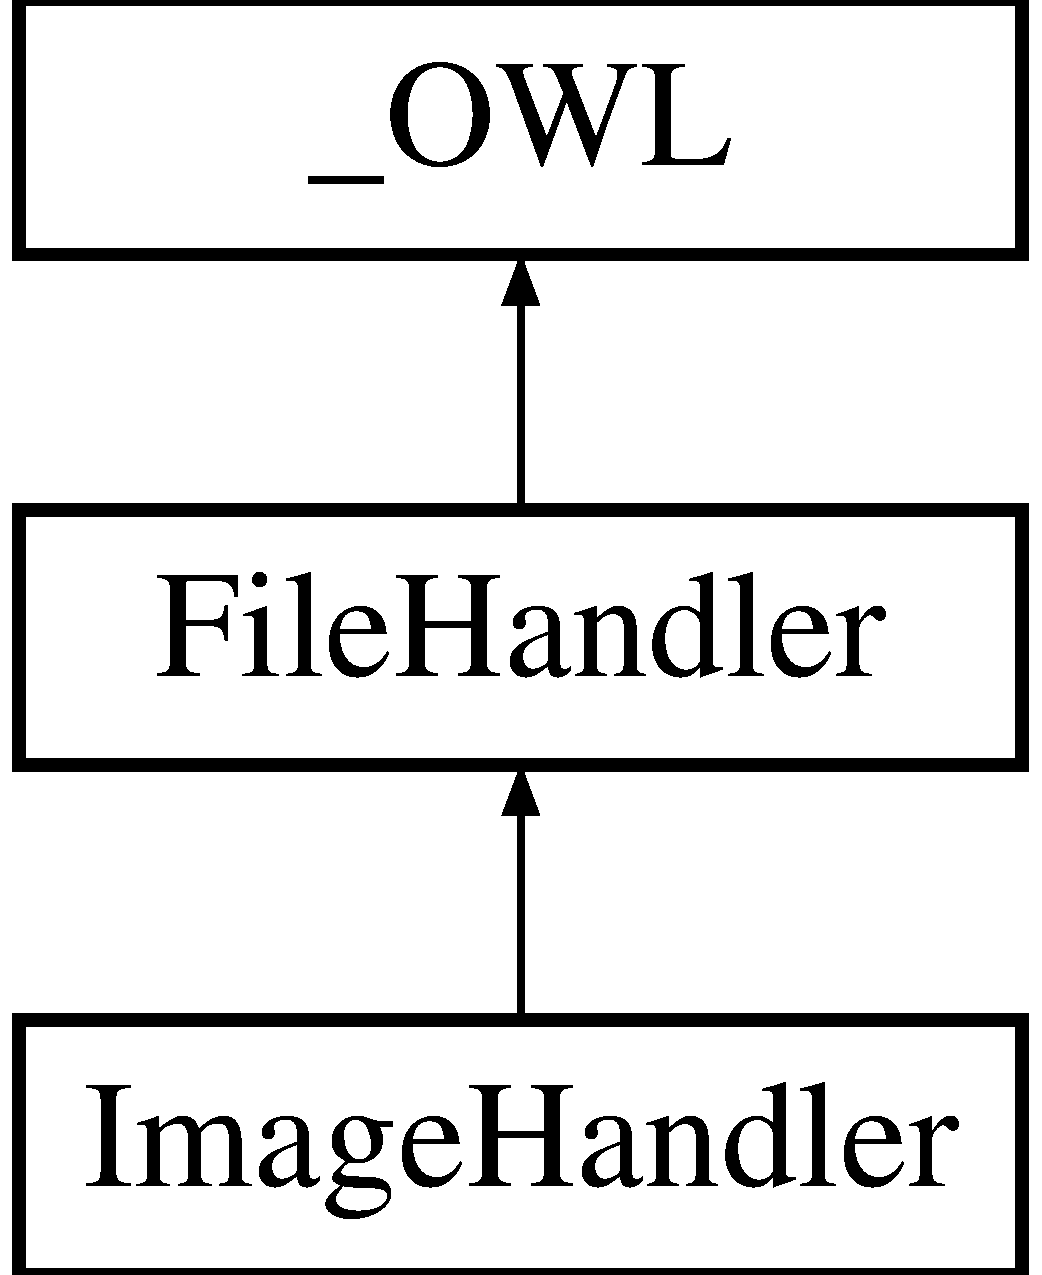
\includegraphics[height=3.000000cm]{classImageHandler}
\end{center}
\end{figure}
\subsection*{Public Member Functions}
\begin{DoxyCompactItemize}
\item 
{\bf \_\-\_\-construct} (\$name, \$req=false)
\item 
{\bf encode} ()
\item 
{\bf download} ()
\item 
{\bf getLastWarning} ()
\item 
{\bf getStatus} ()
\item 
{\bf getSeverity} (\$status=null)
\item 
{\bf succeeded} (\$\_\-ok={\bf OWL\_\-SUCCESS}, \&\$\_\-object=null)
\item 
{\bf signal} (\$level={\bf OWL\_\-INFO}, \&\$text=false)
\item 
{\bf traceback} (\&\$text=false, \$depth=0)
\end{DoxyCompactItemize}
\subsection*{Public Attributes}
\begin{DoxyCompactItemize}
\item 
{\bf \$original\_\-name}
\end{DoxyCompactItemize}
\subsection*{Protected Member Functions}
\begin{DoxyCompactItemize}
\item 
{\bf open} (\$mode= 'r')
\item 
{\bf close} ()
\item 
{\bf readData} ()
\item 
{\bf readLine} (\$trim={\bf FILE\_\-NOTRIM})
\item 
{\bf init} ()
\item 
{\bf setCallback} (\$\_\-dispatcher)
\item 
{\bf setCallbackArgument} (array \$\_\-arg)
\item 
{\bf getCallback} ()
\item 
{\bf reset} ()
\item 
{\bf saveStatus} ()
\item 
{\bf restoreStatus} ()
\item 
{\bf check} (\&\$object, \$level={\bf OWL\_\-WARNING})
\item 
{\bf setStatus} (\$status, \$params=array())
\item 
{\bf setHighSeverity} (\&\$object=null)
\end{DoxyCompactItemize}
\subsection*{Protected Attributes}
\begin{DoxyCompactItemize}
\item 
{\bf \$severity}
\end{DoxyCompactItemize}
\subsection*{Private Attributes}
\begin{DoxyCompactItemize}
\item 
{\bf \$name}
\item 
{\bf \$fpointer}
\item 
{\bf \$opened}
\end{DoxyCompactItemize}


\subsection{Detailed Description}
Image handler. 

Handle all images \begin{DoxyAuthor}{Author}
Oscar van Eijk, Oveas Functionality Provider 
\end{DoxyAuthor}
\begin{DoxyVersion}{Version}
May 15, 2007 -\/-\/ O van Eijk -\/-\/ initial version for Terra-\/Terra (based on an old OFM module) 

Jul 30, 2008 -\/-\/ O van Eijk -\/-\/ Modified version for OWL-\/PHP 
\end{DoxyVersion}


\subsection{Constructor \& Destructor Documentation}
\index{ImageHandler@{ImageHandler}!\_\-\_\-construct@{\_\-\_\-construct}}
\index{\_\-\_\-construct@{\_\-\_\-construct}!ImageHandler@{ImageHandler}}
\subsubsection[{\_\-\_\-construct}]{\setlength{\rightskip}{0pt plus 5cm}ImageHandler::\_\-\_\-construct (
\begin{DoxyParamCaption}
\item[{\$}]{name, }
\item[{\$}]{req = {\ttfamily false}}
\end{DoxyParamCaption}
)}\label{classImageHandler_aa61dc81d4cf98eed31b32e2197018309}
Class constructor; setup the image characteristics 
\begin{DoxyParams}[1]{Parameters}
\mbox{\tt in}  & {\em \$name} & Filename \\
\hline
\mbox{\tt in}  & {\em \$req} & True is the file must exist at object create time \\
\hline
\end{DoxyParams}
\begin{DoxyAuthor}{Author}
Oscar van Eijk, Oveas Functionality Provider 
\end{DoxyAuthor}


Reimplemented from {\bf FileHandler} \doxyref{}{p.}{classFileHandler_a8d75c8ea0c532acdeae0a0a4efa3704a}.



References \$name, \_\-OWL::init(), and \_\-OWL::setStatus().



\subsection{Member Function Documentation}
\index{ImageHandler@{ImageHandler}!check@{check}}
\index{check@{check}!ImageHandler@{ImageHandler}}
\subsubsection[{check}]{\setlength{\rightskip}{0pt plus 5cm}\_\-OWL::check (
\begin{DoxyParamCaption}
\item[{\&\$}]{object, }
\item[{\$}]{level = {\ttfamily {\bf OWL\_\-WARNING}}}
\end{DoxyParamCaption}
)\hspace{0.3cm}{\ttfamily  [protected, inherited]}}\label{class__OWL_ae2e3c56e5f3c4ce4156c6b1bb1c50f63}
This is a helper function for lazy developers. Some checks have to be made quite often, this is a kinda macro to handle that. It compares the own severity level with that of a given object. If the highest level is above a given max, a traceback and reset are performed.


\begin{DoxyParams}[1]{Parameters}
\mbox{\tt in}  & {\em \$object} & Pointer to an object to check against \\
\hline
\mbox{\tt in}  & {\em \$level} & The maximum severity level \\
\hline
\end{DoxyParams}
\begin{DoxyReturn}{Returns}
True if the severity level was correct (below the max), otherwise false 
\end{DoxyReturn}
\begin{DoxyAuthor}{Author}
Oscar van Eijk, Oveas Functionality Provider 
\end{DoxyAuthor}


References \_\-OWL::reset(), \_\-OWL::setHighSeverity(), and \_\-OWL::traceback().



Referenced by SessionHandler::write().

\index{ImageHandler@{ImageHandler}!close@{close}}
\index{close@{close}!ImageHandler@{ImageHandler}}
\subsubsection[{close}]{\setlength{\rightskip}{0pt plus 5cm}FileHandler::close (
\begin{DoxyParamCaption}
{}
\end{DoxyParamCaption}
)\hspace{0.3cm}{\ttfamily  [protected, inherited]}}\label{classFileHandler_aa48e7c3b67346e29b194d2f0ac5dd1f8}
Close the file \begin{DoxyAuthor}{Author}
Oscar van Eijk, Oveas Functionality Provider 
\end{DoxyAuthor}


References \_\-OWL::setStatus().



Referenced by FileHandler::\_\-\_\-destruct(), and FileHandler::readData().

\index{ImageHandler@{ImageHandler}!download@{download}}
\index{download@{download}!ImageHandler@{ImageHandler}}
\subsubsection[{download}]{\setlength{\rightskip}{0pt plus 5cm}FileHandler::download (
\begin{DoxyParamCaption}
{}
\end{DoxyParamCaption}
)\hspace{0.3cm}{\ttfamily  [inherited]}}\label{classFileHandler_ac17edc9b92643c32ae6040b1235c64dd}
\index{ImageHandler@{ImageHandler}!encode@{encode}}
\index{encode@{encode}!ImageHandler@{ImageHandler}}
\subsubsection[{encode}]{\setlength{\rightskip}{0pt plus 5cm}FileHandler::encode (
\begin{DoxyParamCaption}
{}
\end{DoxyParamCaption}
)\hspace{0.3cm}{\ttfamily  [inherited]}}\label{classFileHandler_aa29360bf94fd54d906256561f33d93ad}


References FileHandler::readData().

\index{ImageHandler@{ImageHandler}!getCallback@{getCallback}}
\index{getCallback@{getCallback}!ImageHandler@{ImageHandler}}
\subsubsection[{getCallback}]{\setlength{\rightskip}{0pt plus 5cm}\_\-OWL::getCallback (
\begin{DoxyParamCaption}
{}
\end{DoxyParamCaption}
)\hspace{0.3cm}{\ttfamily  [protected, inherited]}}\label{class__OWL_acb46ff88f43ca66f1268d3f5199c3f8d}
Retrieve a previously set (callback) dispatcher. The (callback) dispatcher is cleared immediatly. \begin{DoxyReturn}{Returns}
The dispatcher, of null on failure. 
\end{DoxyReturn}
\begin{DoxyAuthor}{Author}
Oscar van Eijk, Oveas Functionality Provider 
\end{DoxyAuthor}


Reimplemented in {\bf Dispatcher} \doxyref{}{p.}{classDispatcher_a31c4bd4e4eaee7ef90b1ea364a901447}.



References OWL::factory().

\index{ImageHandler@{ImageHandler}!getLastWarning@{getLastWarning}}
\index{getLastWarning@{getLastWarning}!ImageHandler@{ImageHandler}}
\subsubsection[{getLastWarning}]{\setlength{\rightskip}{0pt plus 5cm}\_\-OWL::getLastWarning (
\begin{DoxyParamCaption}
{}
\end{DoxyParamCaption}
)\hspace{0.3cm}{\ttfamily  [inherited]}}\label{class__OWL_a1888f52fc2d0ec29e146925ccad70a6b}
Get the last warning or error message. \begin{DoxyReturn}{Returns}
null if there was no error (severity below OWL\_\-WARNING), otherwise the error text. 
\end{DoxyReturn}
\begin{DoxyAuthor}{Author}
Oscar van Eijk, Oveas Functionality Provider 
\end{DoxyAuthor}


References \_\-OWL::signal().

\index{ImageHandler@{ImageHandler}!getSeverity@{getSeverity}}
\index{getSeverity@{getSeverity}!ImageHandler@{ImageHandler}}
\subsubsection[{getSeverity}]{\setlength{\rightskip}{0pt plus 5cm}\_\-OWL::getSeverity (
\begin{DoxyParamCaption}
\item[{\$}]{status = {\ttfamily null}}
\end{DoxyParamCaption}
)\hspace{0.3cm}{\ttfamily  [inherited]}}\label{class__OWL_a2374613f9bb7eccf49a5dbc9a9ef4751}
Get the current object severity level. 
\begin{DoxyParams}[1]{Parameters}
\mbox{\tt in}  & {\em \$status} & An optional parameter to check an other status code i.s.o the object's current status. \\
\hline
\end{DoxyParams}
\begin{DoxyReturn}{Returns}
Status severity level 
\end{DoxyReturn}
\begin{DoxyAuthor}{Author}
Oscar van Eijk, Oveas Functionality Provider 
\end{DoxyAuthor}


References \_\-OWL::\$status.



Referenced by LogHandler::composeMessage(), LogHandler::log(), and DataHandler::setKey().

\index{ImageHandler@{ImageHandler}!getStatus@{getStatus}}
\index{getStatus@{getStatus}!ImageHandler@{ImageHandler}}
\subsubsection[{getStatus}]{\setlength{\rightskip}{0pt plus 5cm}\_\-OWL::getStatus (
\begin{DoxyParamCaption}
{}
\end{DoxyParamCaption}
)\hspace{0.3cm}{\ttfamily  [final, inherited]}}\label{class__OWL_ac1f1643ff5b5db7c326c30477603358d}
Get the current object status. \begin{DoxyReturn}{Returns}
Object's status code 
\end{DoxyReturn}
\begin{DoxyAuthor}{Author}
Oscar van Eijk, Oveas Functionality Provider 
\end{DoxyAuthor}


Referenced by SchemeHandler::compare().

\index{ImageHandler@{ImageHandler}!init@{init}}
\index{init@{init}!ImageHandler@{ImageHandler}}
\subsubsection[{init}]{\setlength{\rightskip}{0pt plus 5cm}\_\-OWL::init (
\begin{DoxyParamCaption}
{}
\end{DoxyParamCaption}
)\hspace{0.3cm}{\ttfamily  [protected, inherited]}}\label{class__OWL_ae0ef3ded56e8a6b34b6461e5a721cd3e}
This function should be called by all constuctors. It initializes the general characteristics. Status is 'warning' by default, it's up to the contructor to set a proper status; if it's still 'warning', this $\ast$might$\ast$ indicate something went wrong. \begin{DoxyAuthor}{Author}
Oscar van Eijk, Oveas Functionality Provider 
\end{DoxyAuthor}


References OWL::factory(), and \_\-OWL::setStatus().



Referenced by FormFieldPlugin::\_\-\_\-construct(), Tablerow::\_\-\_\-construct(), Tablecell::\_\-\_\-construct(), Table::\_\-\_\-construct(), Document::\_\-\_\-construct(), ContainerPlugin::\_\-\_\-construct(), Container::\_\-\_\-construct(), SocketHandler::\_\-\_\-construct(), SessionHandler::\_\-\_\-construct(), SchemeHandler::\_\-\_\-construct(), LogHandler::\_\-\_\-construct(), \_\-\_\-construct(), FormHandler::\_\-\_\-construct(), FileHandler::\_\-\_\-construct(), DbHandler::\_\-\_\-construct(), HDataHandler::\_\-\_\-construct(), DataHandler::\_\-\_\-construct(), OWL::\_\-\_\-construct(), Mail::\_\-\_\-construct(), Group::\_\-\_\-construct(), Form::\_\-\_\-construct(), Dispatcher::\_\-\_\-construct(), and User::construct().

\index{ImageHandler@{ImageHandler}!open@{open}}
\index{open@{open}!ImageHandler@{ImageHandler}}
\subsubsection[{open}]{\setlength{\rightskip}{0pt plus 5cm}FileHandler::open (
\begin{DoxyParamCaption}
\item[{\$}]{mode = {\ttfamily 'r'}}
\end{DoxyParamCaption}
)\hspace{0.3cm}{\ttfamily  [protected, inherited]}}\label{classFileHandler_a2a650b033c4eb1f98ba47fb05ce7b454}
Open the file 
\begin{DoxyParams}[1]{Parameters}
\mbox{\tt in}  & {\em \$mode} & Mode in which the file should be opened:
\begin{DoxyItemize}
\item 'r' Open for reading only; place the file pointer at the beginning of the file.
\item 'r+' Open for reading and writing; place the file pointer at the beginning of the file.
\item 'w' Open for writing only; place the file pointer at the beginning of the file and truncate the file to zero length. If the file does not exist, attempt to create it.
\item 'w+' Open for reading and writing; place the file pointer at the beginning of the file and truncate the file to zero length. If the file does not exist, attempt to create it.
\item 'a' Open for writing only; place the file pointer at the end of the file. If the file does not exist, attempt to create it.
\item 'a+' Open for reading and writing; place the file pointer at the end of the file. If the file does not exist, attempt to create it. 
\end{DoxyItemize}\\
\hline
\end{DoxyParams}
\begin{DoxyAuthor}{Author}
Oscar van Eijk, Oveas Functionality Provider 
\end{DoxyAuthor}


References \_\-OWL::setStatus().



Referenced by FileHandler::readData().

\index{ImageHandler@{ImageHandler}!readData@{readData}}
\index{readData@{readData}!ImageHandler@{ImageHandler}}
\subsubsection[{readData}]{\setlength{\rightskip}{0pt plus 5cm}FileHandler::readData (
\begin{DoxyParamCaption}
{}
\end{DoxyParamCaption}
)\hspace{0.3cm}{\ttfamily  [protected, inherited]}}\label{classFileHandler_a6f9263704f08f071a5e563aeb3216d95}
Read the file contents and return as one dataset \begin{DoxyAuthor}{Author}
Oscar van Eijk, Oveas Functionality Provider 
\end{DoxyAuthor}


References FileHandler::close(), and FileHandler::open().



Referenced by FileHandler::encode().

\index{ImageHandler@{ImageHandler}!readLine@{readLine}}
\index{readLine@{readLine}!ImageHandler@{ImageHandler}}
\subsubsection[{readLine}]{\setlength{\rightskip}{0pt plus 5cm}FileHandler::readLine (
\begin{DoxyParamCaption}
\item[{\$}]{trim = {\ttfamily {\bf FILE\_\-NOTRIM}}}
\end{DoxyParamCaption}
)\hspace{0.3cm}{\ttfamily  [protected, inherited]}}\label{classFileHandler_a2140ee43c68f088396b4573a56e3007c}
Read a single line from the file. File must be opened before 
\begin{DoxyParams}[1]{Parameters}
\mbox{\tt in}  & {\em \$trim} & specify how the returned line should be trimmed:
\begin{DoxyItemize}
\item FILE\_\-NOTRIM
\item FILE\_\-TRIM\_\-L
\item FILE\_\-TRIM\_\-R
\item FILE\_\-TRIM\_\-C 
\end{DoxyItemize}\\
\hline
\end{DoxyParams}
\begin{DoxyAuthor}{Author}
Oscar van Eijk, Oveas Functionality Provider 
\end{DoxyAuthor}


References \_\-OWL::setStatus().

\index{ImageHandler@{ImageHandler}!reset@{reset}}
\index{reset@{reset}!ImageHandler@{ImageHandler}}
\subsubsection[{reset}]{\setlength{\rightskip}{0pt plus 5cm}\_\-OWL::reset (
\begin{DoxyParamCaption}
{}
\end{DoxyParamCaption}
)\hspace{0.3cm}{\ttfamily  [protected, inherited]}}\label{class__OWL_a2f2a042bcf31965194c03033df0edc9b}
General reset function for all objects. Should be called after each non-\/fatal error \begin{DoxyAuthor}{Author}
Oscar van Eijk, Oveas Functionality Provider 
\end{DoxyAuthor}


Reimplemented in {\bf DbHandler} \doxyref{}{p.}{classDbHandler_a9982df4830f05803935bb31bac7fae3d}, and {\bf SchemeHandler} \doxyref{}{p.}{classSchemeHandler_aa25feb4a70d67b3d571904be4b2f50bc}.



References \_\-OWL::resetCalltree().



Referenced by \_\-OWL::check(), SessionHandler::read(), DataHandler::reset(), and \_\-OWL::setStatus().

\index{ImageHandler@{ImageHandler}!restoreStatus@{restoreStatus}}
\index{restoreStatus@{restoreStatus}!ImageHandler@{ImageHandler}}
\subsubsection[{restoreStatus}]{\setlength{\rightskip}{0pt plus 5cm}\_\-OWL::restoreStatus (
\begin{DoxyParamCaption}
{}
\end{DoxyParamCaption}
)\hspace{0.3cm}{\ttfamily  [protected, inherited]}}\label{class__OWL_a93de01a9bbbc3f228e1a62a0740e90f0}
Restore the previously saved status object and destroy the copy \begin{DoxyAuthor}{Author}
Oscar van Eijk, Oveas Functionality Provider 
\end{DoxyAuthor}


References \_\-OWL::setStatus().



Referenced by User::logout().

\index{ImageHandler@{ImageHandler}!saveStatus@{saveStatus}}
\index{saveStatus@{saveStatus}!ImageHandler@{ImageHandler}}
\subsubsection[{saveStatus}]{\setlength{\rightskip}{0pt plus 5cm}\_\-OWL::saveStatus (
\begin{DoxyParamCaption}
{}
\end{DoxyParamCaption}
)\hspace{0.3cm}{\ttfamily  [protected, inherited]}}\label{class__OWL_add923dc756471318edca8883db3f4420}
Create a copy of the status object \begin{DoxyAuthor}{Author}
Oscar van Eijk, Oveas Functionality Provider 
\end{DoxyAuthor}


Referenced by User::logout().

\index{ImageHandler@{ImageHandler}!setCallback@{setCallback}}
\index{setCallback@{setCallback}!ImageHandler@{ImageHandler}}
\subsubsection[{setCallback}]{\setlength{\rightskip}{0pt plus 5cm}\_\-OWL::setCallback (
\begin{DoxyParamCaption}
\item[{\$}]{\_\-dispatcher}
\end{DoxyParamCaption}
)\hspace{0.3cm}{\ttfamily  [protected, inherited]}}\label{class__OWL_a5f84d43cd4dc7810649f1e2ebecad360}
Set a dispatcher for later callback 
\begin{DoxyParams}[1]{Parameters}
\mbox{\tt in}  & {\em \$\_\-dispatcher} & Dispatched, \\
\hline
\end{DoxyParams}
\begin{DoxySeeAlso}{See also}
\doxyref{Dispatcher::composeDispatcher()}{p.}{classDispatcher_a8a974bbbb30be7cda74f9929972fd2f6} 
\end{DoxySeeAlso}
\begin{DoxyReturn}{Returns}
True on success, false on failure 
\end{DoxyReturn}
\begin{DoxyAuthor}{Author}
Oscar van Eijk, Oveas Functionality Provider 
\end{DoxyAuthor}


References OWL::factory().

\index{ImageHandler@{ImageHandler}!setCallbackArgument@{setCallbackArgument}}
\index{setCallbackArgument@{setCallbackArgument}!ImageHandler@{ImageHandler}}
\subsubsection[{setCallbackArgument}]{\setlength{\rightskip}{0pt plus 5cm}\_\-OWL::setCallbackArgument (
\begin{DoxyParamCaption}
\item[{array \$}]{\_\-arg}
\end{DoxyParamCaption}
)\hspace{0.3cm}{\ttfamily  [protected, inherited]}}\label{class__OWL_a4e9ebfbd3c0d76539bed4e44de9962c3}
Add an argument to a previously registered callback dispatcher 
\begin{DoxyParams}[1]{Parameters}
\mbox{\tt in}  & {\em \$\_\-arg} & Argument, must be an array type. When non-\/ arrays should be passed as arguments, the must be set when the callback is registered already \\
\hline
\end{DoxyParams}
\begin{DoxyReturn}{Returns}
True on success, false on failure 
\end{DoxyReturn}
\begin{DoxyAuthor}{Author}
Oscar van Eijk, Oveas Functionality Provider 
\end{DoxyAuthor}


References OWL::factory().



Referenced by User::register().

\index{ImageHandler@{ImageHandler}!setHighSeverity@{setHighSeverity}}
\index{setHighSeverity@{setHighSeverity}!ImageHandler@{ImageHandler}}
\subsubsection[{setHighSeverity}]{\setlength{\rightskip}{0pt plus 5cm}\_\-OWL::setHighSeverity (
\begin{DoxyParamCaption}
\item[{\&\$}]{object = {\ttfamily null}}
\end{DoxyParamCaption}
)\hspace{0.3cm}{\ttfamily  [protected, inherited]}}\label{class__OWL_a97173dbe452428d3851406413264734d}
Compare the severity level of the current object with a given one and set my statuspointer to the object with the highest level. \begin{DoxyAuthor}{Author}
Oscar van Eijk, Oveas Functionality Provider 
\end{DoxyAuthor}


Referenced by \_\-OWL::check(), DataHandler::db(), DataHandler::prepare(), and SessionHandler::read().

\index{ImageHandler@{ImageHandler}!setStatus@{setStatus}}
\index{setStatus@{setStatus}!ImageHandler@{ImageHandler}}
\subsubsection[{setStatus}]{\setlength{\rightskip}{0pt plus 5cm}\_\-OWL::setStatus (
\begin{DoxyParamCaption}
\item[{\$}]{status, }
\item[{\$}]{params = {\ttfamily array~()}}
\end{DoxyParamCaption}
)\hspace{0.3cm}{\ttfamily  [final, protected, inherited]}}\label{class__OWL_a80e2fe01c3663dbb0ab685eebe33fd1e}
Set the current object status to the specified value. 
\begin{DoxyParams}[1]{Parameters}
\mbox{\tt in}  & {\em \$status} & \doxyref{OWL}{p.}{classOWL} status code \\
\hline
\mbox{\tt in}  & {\em \$params} & \\
\hline
\end{DoxyParams}
\begin{DoxyAuthor}{Author}
Oscar van Eijk, Oveas Functionality Provider 
\end{DoxyAuthor}


References \$GLOBALS, \_\-OWL::\$status, ConfigHandler::get(), Register::getCode(), \_\-OWL::reset(), and \_\-OWL::signal().



Referenced by DbHandler::\_\-\_\-clone(), Container::\_\-\_\-construct(), SocketHandler::\_\-\_\-construct(), SchemeHandler::\_\-\_\-construct(), \_\-\_\-construct(), FormHandler::\_\-\_\-construct(), FileHandler::\_\-\_\-construct(), DbHandler::\_\-\_\-construct(), DataHandler::\_\-\_\-construct(), Session::\_\-\_\-construct(), Mail::\_\-\_\-construct(), BaseElement::\_\-getContent(), HDataHandler::\_\-getNewLeft(), Mail::addBcc(), Mail::addCc(), Form::addField(), FormFieldRadioPlugin::addOption(), HDataHandler::addParent(), Mail::addTo(), BaseElement::addToContent(), DbHandler::alt(), SchemeHandler::alterScheme(), FileHandler::close(), DbHandler::commitTransaction(), Dispatcher::composeDispatcher(), User::confirm(), SocketHandler::connect(), DbHandler::connect(), DbHandler::create(), SchemeHandler::createScheme(), SchemeHandler::defineIndex(), SchemeHandler::defineScheme(), SocketHandler::disconnect(), Dispatcher::dispatch(), HDataHandler::enableCrossLink(), FormHandler::get(), DataHandler::get(), HDataHandler::getDirectChildren(), HDataHandler::getFullOffspring(), SchemeHandler::getTableColumns(), SchemeHandler::getTableIndexes(), \_\-OWL::init(), Document::loadScript(), Document::loadStyle(), DbHandler::lockTable(), User::login(), HDataHandler::moveNode(), FileHandler::open(), DbHandler::open(), LogHandler::openLogfile(), DataHandler::prepare(), DbHandler::prepareDelete(), DbHandler::prepareField(), DbHandler::prepareInsert(), DbHandler::prepareRead(), DbHandler::prepareUpdate(), SocketHandler::read(), DbHandler::read(), FileHandler::readLine(), HDataHandler::readQuery(), User::readUserdata(), User::register(), Dispatcher::registerArgument(), Dispatcher::registerCallback(), \_\-OWL::restoreStatus(), DbHandler::rollbackTransaction(), SchemeHandler::scheme(), Mail::send(), FormHandler::set(), BaseElement::setAttributes(), BaseElement::setContent(), Form::setEncoding(), Document::setFavicon(), Form::setFieldAttributes(), Mail::setFrom(), DataHandler::setJoin(), DataHandler::setKey(), FormFieldTextPlugin::setMaxsize(), Document::setMeta(), Form::setMethod(), FormFieldRadioPlugin::setSelected(), Mail::setSender(), FormFieldTextPlugin::setSize(), FormFieldSelectPlugin::setSize(), FormFieldSelectPlugin::setValue(), Form::showField(), DbHandler::startTransaction(), SchemeHandler::tableDescription(), DbHandler::unlockTable(), SchemeHandler::validateScheme(), SocketHandler::write(), DbHandler::write(), and HDataHandler::writeQuery().

\index{ImageHandler@{ImageHandler}!signal@{signal}}
\index{signal@{signal}!ImageHandler@{ImageHandler}}
\subsubsection[{signal}]{\setlength{\rightskip}{0pt plus 5cm}\_\-OWL::signal (
\begin{DoxyParamCaption}
\item[{\$}]{level = {\ttfamily {\bf OWL\_\-INFO}}, }
\item[{\&\$}]{text = {\ttfamily false}}
\end{DoxyParamCaption}
)\hspace{0.3cm}{\ttfamily  [inherited]}}\label{class__OWL_a51ba4a16409acf2a2f61f286939091a5}
Display the message for the current object status 
\begin{DoxyParams}[1]{Parameters}
\mbox{\tt in}  & {\em \$level} & An optional severity level; message will only be displayed when it is at least of this level. \\
\hline
\mbox{\tt out}  & {\em \$text} & If this parameter is given, the message text is returned in this string instead of echood. \\
\hline
\end{DoxyParams}
\begin{DoxyReturn}{Returns}
The severity level for this object 
\end{DoxyReturn}
\begin{DoxyAuthor}{Author}
Oscar van Eijk, Oveas Functionality Provider 
\end{DoxyAuthor}


References ConfigHandler::get().



Referenced by \_\-OWL::getLastWarning(), \_\-OWL::setStatus(), and \_\-OWL::traceback().

\index{ImageHandler@{ImageHandler}!succeeded@{succeeded}}
\index{succeeded@{succeeded}!ImageHandler@{ImageHandler}}
\subsubsection[{succeeded}]{\setlength{\rightskip}{0pt plus 5cm}\_\-OWL::succeeded (
\begin{DoxyParamCaption}
\item[{\$}]{\_\-ok = {\ttfamily {\bf OWL\_\-SUCCESS}}, }
\item[{\&\$}]{\_\-object = {\ttfamily null}}
\end{DoxyParamCaption}
)\hspace{0.3cm}{\ttfamily  [inherited]}}\label{class__OWL_a53ab4d3bbb2c6a56966c339ca4b4c805}
Check if the object currenlty has a success state 
\begin{DoxyParams}[1]{Parameters}
\mbox{\tt in}  & {\em \$\_\-ok} & The highest severity that's considered successfull, default OWL\_\-SUCCESS \\
\hline
\mbox{\tt in}  & {\em \$\_\-object} & REference to the object to check, defaults to the current object \\
\hline
\end{DoxyParams}
\begin{DoxyReturn}{Returns}
Boolean true when successfull 
\end{DoxyReturn}
\begin{DoxyAuthor}{Author}
Oscar van Eijk, Oveas Functionality Provider 
\end{DoxyAuthor}


Referenced by User::construct(), Dispatcher::registerArgument(), and Dispatcher::registerCallback().

\index{ImageHandler@{ImageHandler}!traceback@{traceback}}
\index{traceback@{traceback}!ImageHandler@{ImageHandler}}
\subsubsection[{traceback}]{\setlength{\rightskip}{0pt plus 5cm}\_\-OWL::traceback (
\begin{DoxyParamCaption}
\item[{\&\$}]{text = {\ttfamily false}, }
\item[{\$}]{depth = {\ttfamily 0}}
\end{DoxyParamCaption}
)\hspace{0.3cm}{\ttfamily  [inherited]}}\label{class__OWL_aa29547995d6741b7d2b90c1d4ea99a13}
If somehwere in the nested calls an error occured, we can traceback the original failing object with this function and signal the message. 
\begin{DoxyParams}[1]{Parameters}
\mbox{\tt out}  & {\em \$text} & Optional variable in which the message text can be stored. If not given, the text will be written to standard output \\
\hline
\mbox{\tt in}  & {\em \$depth} & This paramater should be initially empty. It calculates the depth in recursive calls. \\
\hline
\end{DoxyParams}
\begin{DoxyReturn}{Returns}
Severity code of the failing object 
\end{DoxyReturn}
\begin{DoxyAuthor}{Author}
Oscar van Eijk, Oveas Functionality Provider 
\end{DoxyAuthor}


References \_\-OWL::signal().



Referenced by \_\-OWL::check(), User::login(), and SessionHandler::read().



\subsection{Member Data Documentation}
\index{ImageHandler@{ImageHandler}!\$fpointer@{\$fpointer}}
\index{\$fpointer@{\$fpointer}!ImageHandler@{ImageHandler}}
\subsubsection[{\$fpointer}]{\setlength{\rightskip}{0pt plus 5cm}ImageHandler::\$fpointer\hspace{0.3cm}{\ttfamily  [private]}}\label{classImageHandler_ac56acda82f7ece75d33f6c57845a727e}
Pointer to te file when opened 

Reimplemented from {\bf FileHandler} \doxyref{}{p.}{classFileHandler_aa0aa66fd3ad551b3f508b901a95c0c2d}.

\index{ImageHandler@{ImageHandler}!\$name@{\$name}}
\index{\$name@{\$name}!ImageHandler@{ImageHandler}}
\subsubsection[{\$name}]{\setlength{\rightskip}{0pt plus 5cm}ImageHandler::\$name\hspace{0.3cm}{\ttfamily  [private]}}\label{classImageHandler_a517b3d7ff8643cca1dc2080523bfe2d6}
Full filename as stored on the file system 

Reimplemented from {\bf FileHandler} \doxyref{}{p.}{classFileHandler_a94903bd51b241928ed415ad271c38805}.



Referenced by \_\-\_\-construct().

\index{ImageHandler@{ImageHandler}!\$opened@{\$opened}}
\index{\$opened@{\$opened}!ImageHandler@{ImageHandler}}
\subsubsection[{\$opened}]{\setlength{\rightskip}{0pt plus 5cm}ImageHandler::\$opened\hspace{0.3cm}{\ttfamily  [private]}}\label{classImageHandler_a6a87b3626bd0a457c6937b3e9b1cc69b}
Boolean that's true when the file is opened 

Reimplemented from {\bf FileHandler} \doxyref{}{p.}{classFileHandler_a061409b2bbd2e13bc47415527c0de720}.

\index{ImageHandler@{ImageHandler}!\$original\_\-name@{\$original\_\-name}}
\index{\$original\_\-name@{\$original\_\-name}!ImageHandler@{ImageHandler}}
\subsubsection[{\$original\_\-name}]{\setlength{\rightskip}{0pt plus 5cm}ImageHandler::\$original\_\-name}\label{classImageHandler_a1712c9444d65879aab111260767afaab}


Reimplemented from {\bf FileHandler} \doxyref{}{p.}{classFileHandler_a477708585850c3c8725ccf56bfe0b4a8}.

\index{ImageHandler@{ImageHandler}!\$severity@{\$severity}}
\index{\$severity@{\$severity}!ImageHandler@{ImageHandler}}
\subsubsection[{\$severity}]{\setlength{\rightskip}{0pt plus 5cm}\_\-OWL::\$severity\hspace{0.3cm}{\ttfamily  [protected, inherited]}}\label{class__OWL_ad26b40a9dbbacb33e299b17826f8327c}
Severity level of the current object status 

The documentation for this class was generated from the following file:\begin{DoxyCompactItemize}
\item 
/home/oscar/projects/owl-\/php/src/kernel/so/{\bf class.imagehandler.php}\end{DoxyCompactItemize}

\hypertarget{classLogHandler}{
\section{LogHandler Class Reference}
\label{classLogHandler}\index{LogHandler@{LogHandler}}
}
Log handler.  


Inheritance diagram for LogHandler:\nopagebreak
\begin{figure}[H]
\begin{center}
\leavevmode
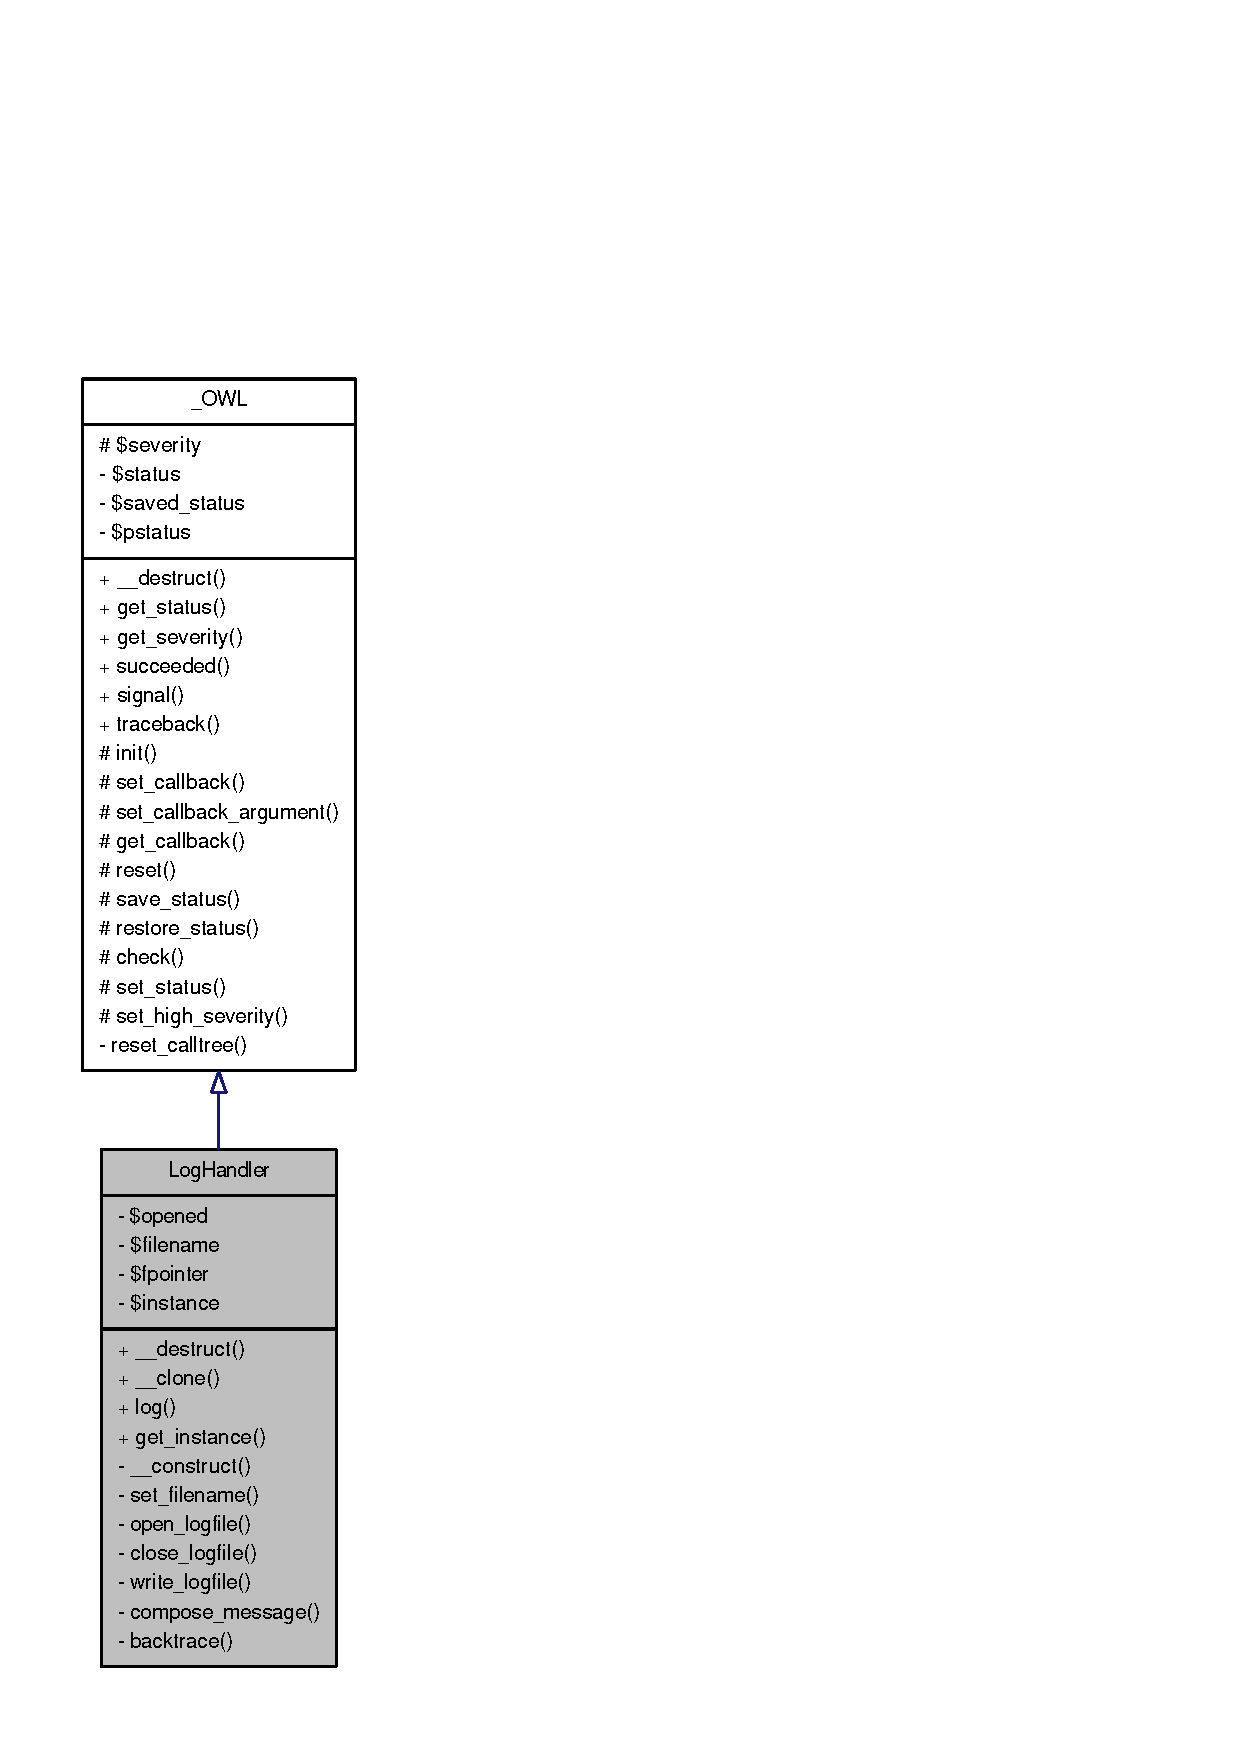
\includegraphics[width=70pt]{classLogHandler__inherit__graph}
\end{center}
\end{figure}
Collaboration diagram for LogHandler:\nopagebreak
\begin{figure}[H]
\begin{center}
\leavevmode
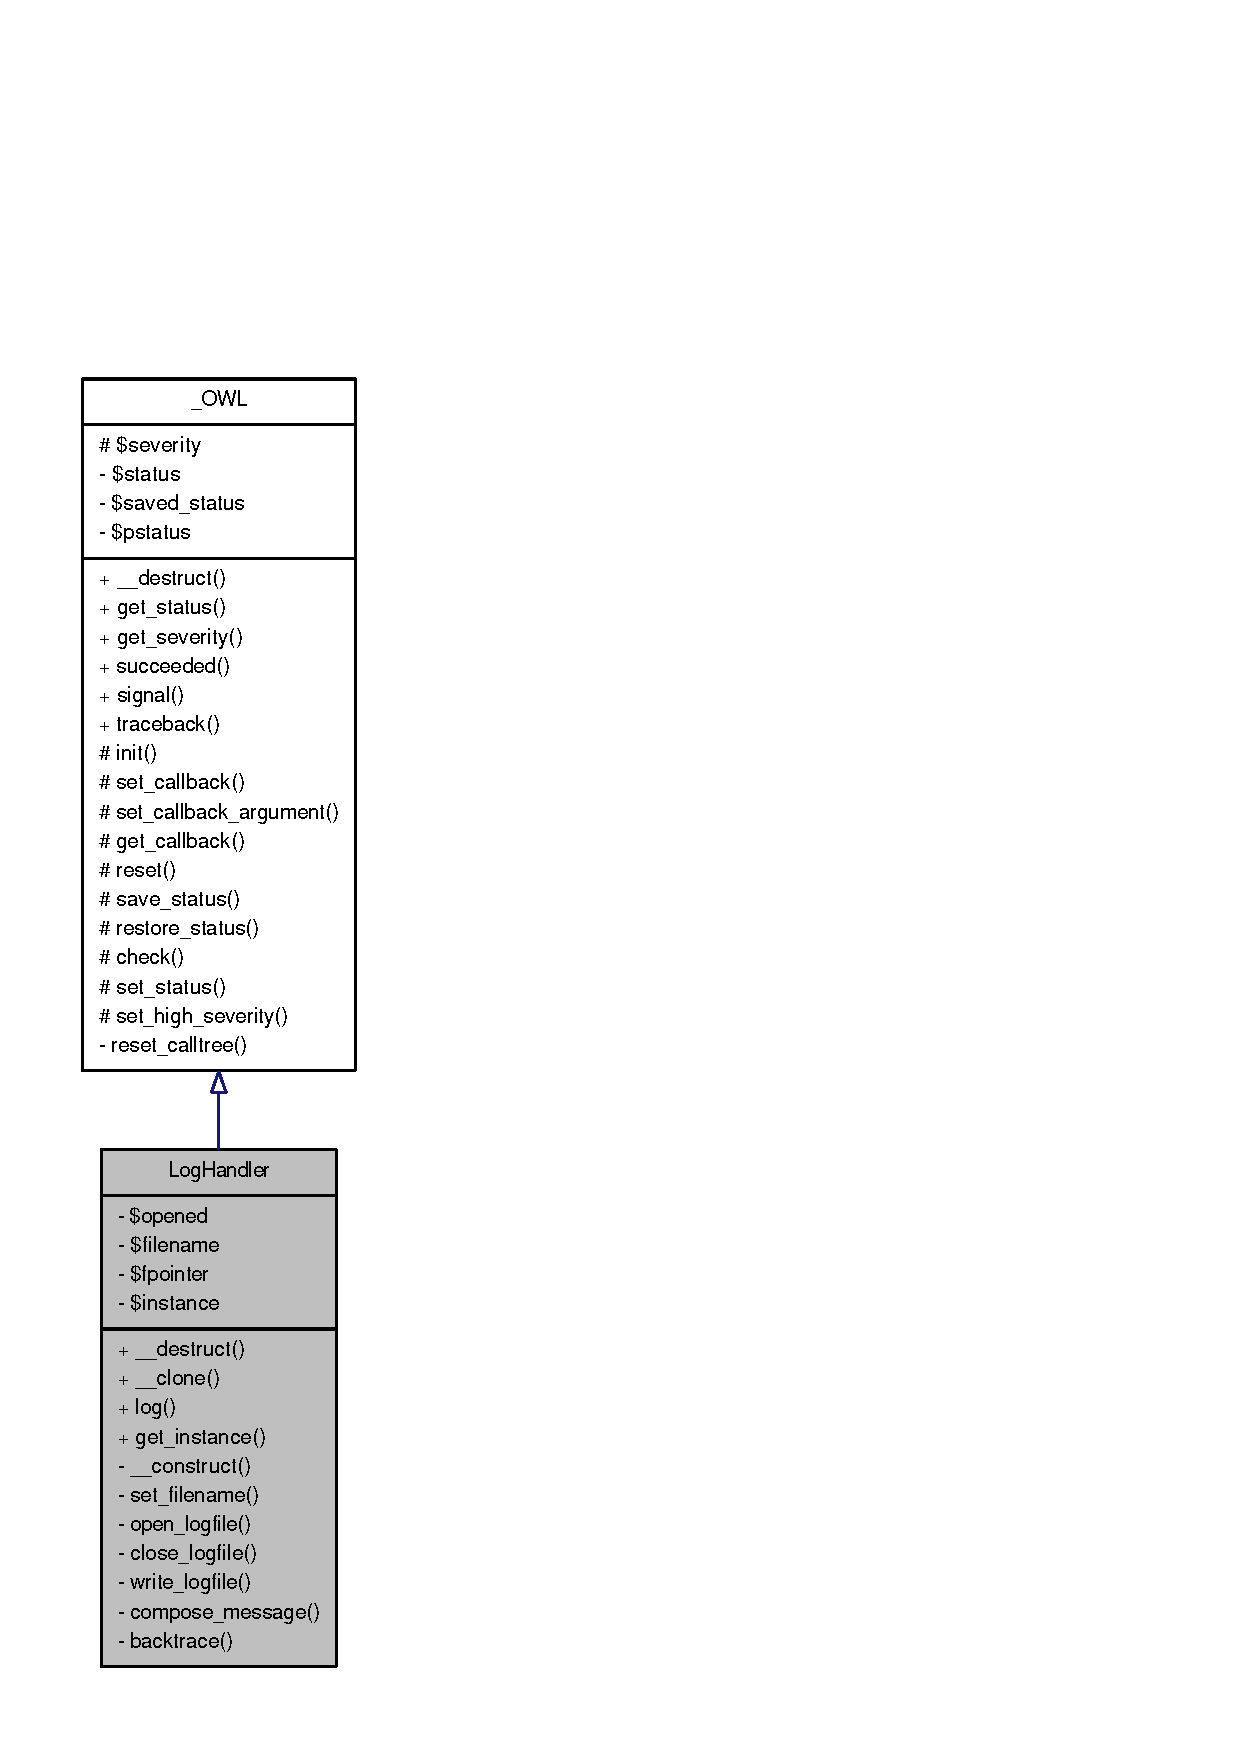
\includegraphics[width=70pt]{classLogHandler__coll__graph}
\end{center}
\end{figure}
\subsection*{Public Member Functions}
\begin{CompactItemize}
\item 
\hyperlink{classLogHandler_acca49c4394109f4ccc494048a0b2cab}{\_\-\_\-construct} ()
\item 
\hyperlink{classLogHandler_acd0c653489cf221423b9edd62e81458}{\_\-\_\-destruct} ()
\end{CompactItemize}
\subsection*{Protected Member Functions}
\begin{CompactItemize}
\item 
\hyperlink{class__OWL_e0ef3ded56e8a6b34b6461e5a721cd3e}{init} ()
\item 
\hyperlink{class__OWL_2f2a042bcf31965194c03033df0edc9b}{reset} ()
\end{CompactItemize}
\subsection*{Private Member Functions}
\begin{CompactItemize}
\item 
\hyperlink{classLogHandler_65ef4f1c6ab4cff4057f5f5932cc690e}{set\_\-filename} ()
\item 
\hyperlink{classLogHandler_af324e5156bf8ea83e5b4e990ea99e2d}{open\_\-logfile} ()
\item 
\hyperlink{classLogHandler_1a3b03d9bb97404a4f746bd2aacc5a8c}{close\_\-logfile} ()
\item 
\hyperlink{classLogHandler_e0cd68fb6f068e47f899a1e4c7f29ba9}{write\_\-logfile} (\$msg)
\end{CompactItemize}
\subsection*{Private Attributes}
\begin{CompactItemize}
\item 
\hyperlink{classLogHandler_956e7e71a9ff96c6301d1f41a5bf207e}{\$opened}
\item 
\hyperlink{classLogHandler_b51c12bcd654093b9d0153ab38ebad8c}{\$filename}
\item 
\hyperlink{classLogHandler_d65c8954bda40d8a33828f0a0a2cbf5b}{\$fpointer}
\end{CompactItemize}


\subsection{Detailed Description}
Log handler. 

This class handles all \hyperlink{classOWL}{OWL} logging \begin{Desc}
\item[Author:]Oscar van Eijk, Oveas Functionality Provider \end{Desc}
\begin{Desc}
\item[Version:]Aug 13, 2008 -- O van Eijk -- initial version \end{Desc}


\subsection{Constructor \& Destructor Documentation}
\hypertarget{classLogHandler_acca49c4394109f4ccc494048a0b2cab}{
\index{LogHandler@{LogHandler}!\_\-\_\-construct@{\_\-\_\-construct}}
\index{\_\-\_\-construct@{\_\-\_\-construct}!LogHandler@{LogHandler}}
\subsubsection{\setlength{\rightskip}{0pt plus 5cm}LogHandler::\_\-\_\-construct ()}}
\label{classLogHandler_acca49c4394109f4ccc494048a0b2cab}


Class constructor \hypertarget{classLogHandler_acd0c653489cf221423b9edd62e81458}{
\index{LogHandler@{LogHandler}!\_\-\_\-destruct@{\_\-\_\-destruct}}
\index{\_\-\_\-destruct@{\_\-\_\-destruct}!LogHandler@{LogHandler}}
\subsubsection{\setlength{\rightskip}{0pt plus 5cm}LogHandler::\_\-\_\-destruct ()}}
\label{classLogHandler_acd0c653489cf221423b9edd62e81458}


Class destructor 

Reimplemented from \hyperlink{class__OWL_44fd2222476a3109286cc82d92b6bbcc}{\_\-OWL}.

\subsection{Member Function Documentation}
\hypertarget{classLogHandler_65ef4f1c6ab4cff4057f5f5932cc690e}{
\index{LogHandler@{LogHandler}!set\_\-filename@{set\_\-filename}}
\index{set\_\-filename@{set\_\-filename}!LogHandler@{LogHandler}}
\subsubsection{\setlength{\rightskip}{0pt plus 5cm}LogHandler::set\_\-filename ()\hspace{0.3cm}{\tt  \mbox{[}private\mbox{]}}}}
\label{classLogHandler_65ef4f1c6ab4cff4057f5f5932cc690e}


Find out what the filename of the logfile should be \hypertarget{classLogHandler_af324e5156bf8ea83e5b4e990ea99e2d}{
\index{LogHandler@{LogHandler}!open\_\-logfile@{open\_\-logfile}}
\index{open\_\-logfile@{open\_\-logfile}!LogHandler@{LogHandler}}
\subsubsection{\setlength{\rightskip}{0pt plus 5cm}LogHandler::open\_\-logfile ()\hspace{0.3cm}{\tt  \mbox{[}private\mbox{]}}}}
\label{classLogHandler_af324e5156bf8ea83e5b4e990ea99e2d}


Open the logfile for write \hypertarget{classLogHandler_1a3b03d9bb97404a4f746bd2aacc5a8c}{
\index{LogHandler@{LogHandler}!close\_\-logfile@{close\_\-logfile}}
\index{close\_\-logfile@{close\_\-logfile}!LogHandler@{LogHandler}}
\subsubsection{\setlength{\rightskip}{0pt plus 5cm}LogHandler::close\_\-logfile ()\hspace{0.3cm}{\tt  \mbox{[}private\mbox{]}}}}
\label{classLogHandler_1a3b03d9bb97404a4f746bd2aacc5a8c}


Close the logfile \hypertarget{classLogHandler_e0cd68fb6f068e47f899a1e4c7f29ba9}{
\index{LogHandler@{LogHandler}!write\_\-logfile@{write\_\-logfile}}
\index{write\_\-logfile@{write\_\-logfile}!LogHandler@{LogHandler}}
\subsubsection{\setlength{\rightskip}{0pt plus 5cm}LogHandler::write\_\-logfile (\$ {\em msg})\hspace{0.3cm}{\tt  \mbox{[}private\mbox{]}}}}
\label{classLogHandler_e0cd68fb6f068e47f899a1e4c7f29ba9}


Write a message to the logfile

\begin{Desc}
\item[Parameters:]
\begin{description}
\item[\mbox{$\leftarrow$} {\em \$msg}]The complete log message \end{description}
\end{Desc}
\hypertarget{class__OWL_e0ef3ded56e8a6b34b6461e5a721cd3e}{
\index{LogHandler@{LogHandler}!init@{init}}
\index{init@{init}!LogHandler@{LogHandler}}
\subsubsection{\setlength{\rightskip}{0pt plus 5cm}\_\-OWL::init ()\hspace{0.3cm}{\tt  \mbox{[}protected, inherited\mbox{]}}}}
\label{class__OWL_e0ef3ded56e8a6b34b6461e5a721cd3e}


This function should be called by all constuctors. It initializes the general characteristics. Status is 'warning' by default, it's up to the contructor to set a proper status; if it's still 'warning', this $\ast$might$\ast$ indicate something went wrong. \hypertarget{class__OWL_2f2a042bcf31965194c03033df0edc9b}{
\index{LogHandler@{LogHandler}!reset@{reset}}
\index{reset@{reset}!LogHandler@{LogHandler}}
\subsubsection{\setlength{\rightskip}{0pt plus 5cm}\_\-OWL::reset ()\hspace{0.3cm}{\tt  \mbox{[}protected, inherited\mbox{]}}}}
\label{class__OWL_2f2a042bcf31965194c03033df0edc9b}


General reset function for all objects. Should be called after each non-fatal error 

Reimplemented in \hyperlink{classDbHandler_9982df4830f05803935bb31bac7fae3d}{DbHandler}.

\subsection{Member Data Documentation}
\hypertarget{classLogHandler_956e7e71a9ff96c6301d1f41a5bf207e}{
\index{LogHandler@{LogHandler}!\$opened@{\$opened}}
\index{\$opened@{\$opened}!LogHandler@{LogHandler}}
\subsubsection{\setlength{\rightskip}{0pt plus 5cm}LogHandler::\$opened\hspace{0.3cm}{\tt  \mbox{[}private\mbox{]}}}}
\label{classLogHandler_956e7e71a9ff96c6301d1f41a5bf207e}


Boolean to keep track of the logfile status \hypertarget{classLogHandler_b51c12bcd654093b9d0153ab38ebad8c}{
\index{LogHandler@{LogHandler}!\$filename@{\$filename}}
\index{\$filename@{\$filename}!LogHandler@{LogHandler}}
\subsubsection{\setlength{\rightskip}{0pt plus 5cm}LogHandler::\$filename\hspace{0.3cm}{\tt  \mbox{[}private\mbox{]}}}}
\label{classLogHandler_b51c12bcd654093b9d0153ab38ebad8c}


Name of the logfile \hypertarget{classLogHandler_d65c8954bda40d8a33828f0a0a2cbf5b}{
\index{LogHandler@{LogHandler}!\$fpointer@{\$fpointer}}
\index{\$fpointer@{\$fpointer}!LogHandler@{LogHandler}}
\subsubsection{\setlength{\rightskip}{0pt plus 5cm}LogHandler::\$fpointer\hspace{0.3cm}{\tt  \mbox{[}private\mbox{]}}}}
\label{classLogHandler_d65c8954bda40d8a33828f0a0a2cbf5b}


File pointer 

The documentation for this class was generated from the following file:\begin{CompactItemize}
\item 
/home/oscar/work/eclipse/owl-php/src/kernel/so/\hyperlink{class_8loghandler_8php}{class.loghandler.php}\end{CompactItemize}

\section{OldOFMStuff Class Reference}
\label{classOldOFMStuff}\index{OldOFMStuff@{OldOFMStuff}}
\subsection*{Public Member Functions}
\begin{DoxyCompactItemize}
\item 
\hyperlink{classOldOFMStuff_af1e0b3594d0067d2a1521e433e953d31}{OFM\_\-FileDetails} (\$Path, \$File)
\item 
\hyperlink{classOldOFMStuff_a3581c36a611c8ef33f7a16789cec9d5d}{OFM\_\-FileInfo} (\$Path, \$File)
\item 
\hyperlink{classOldOFMStuff_a5ba4191cf6b199f40bc9209a6e67a119}{OFM\_\-IsAscii} (\$File, \$Type)
\end{DoxyCompactItemize}


\subsection{Member Function Documentation}
\index{OldOFMStuff@{OldOFMStuff}!OFM\_\-FileDetails@{OFM\_\-FileDetails}}
\index{OFM\_\-FileDetails@{OFM\_\-FileDetails}!OldOFMStuff@{OldOFMStuff}}
\subsubsection[{OFM\_\-FileDetails}]{\setlength{\rightskip}{0pt plus 5cm}OldOFMStuff::OFM\_\-FileDetails (\$ {\em Path}, \/  \$ {\em File})}\label{classOldOFMStuff_af1e0b3594d0067d2a1521e433e953d31}


References OFM\_\-FileInfo().

\index{OldOFMStuff@{OldOFMStuff}!OFM\_\-FileInfo@{OFM\_\-FileInfo}}
\index{OFM\_\-FileInfo@{OFM\_\-FileInfo}!OldOFMStuff@{OldOFMStuff}}
\subsubsection[{OFM\_\-FileInfo}]{\setlength{\rightskip}{0pt plus 5cm}OldOFMStuff::OFM\_\-FileInfo (\$ {\em Path}, \/  \$ {\em File})}\label{classOldOFMStuff_a3581c36a611c8ef33f7a16789cec9d5d}


References OFM\_\-IsAscii().



Referenced by OFM\_\-FileDetails().

\index{OldOFMStuff@{OldOFMStuff}!OFM\_\-IsAscii@{OFM\_\-IsAscii}}
\index{OFM\_\-IsAscii@{OFM\_\-IsAscii}!OldOFMStuff@{OldOFMStuff}}
\subsubsection[{OFM\_\-IsAscii}]{\setlength{\rightskip}{0pt plus 5cm}OldOFMStuff::OFM\_\-IsAscii (\$ {\em File}, \/  \$ {\em Type})}\label{classOldOFMStuff_a5ba4191cf6b199f40bc9209a6e67a119}


Referenced by OFM\_\-FileInfo().



The documentation for this class was generated from the following file:\begin{DoxyCompactItemize}
\item 
/home/oscar/projects/owl-\/php/src/kernel/so/\hyperlink{class_8filehandler_8php}{class.filehandler.php}\end{DoxyCompactItemize}

\section{OWL Class Reference}
\label{classOWL}\index{OWL@{OWL}}
Inheritance diagram for OWL:\begin{figure}[H]
\begin{center}
\leavevmode
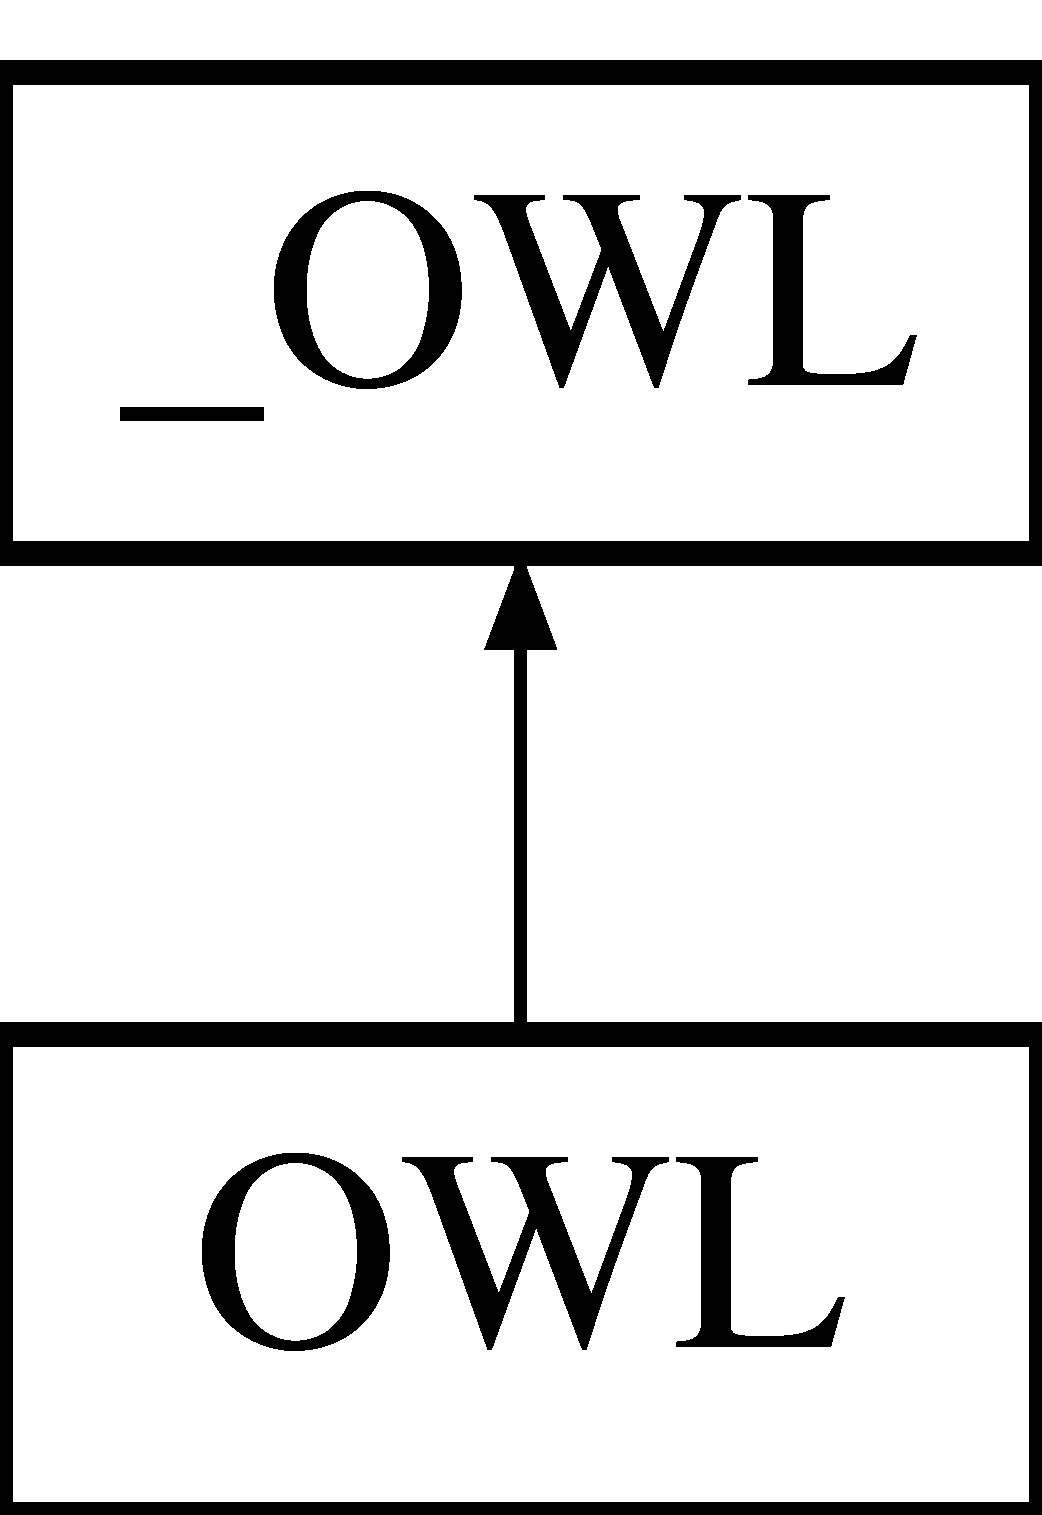
\includegraphics[height=2.000000cm]{classOWL}
\end{center}
\end{figure}
\subsection*{Public Member Functions}
\begin{DoxyCompactItemize}
\item 
{\bf \_\-\_\-clone} ()
\item 
{\bf getStatus} ()
\item 
{\bf getSeverity} (\$status=null)
\item 
{\bf succeeded} (\$\_\-ok={\bf OWL\_\-SUCCESS}, \&\$\_\-object=null)
\item 
{\bf signal} (\$level={\bf OWL\_\-INFO}, \&\$text=false)
\item 
{\bf traceback} (\&\$text=false, \$depth=0)
\end{DoxyCompactItemize}
\subsection*{Static Public Member Functions}
\begin{DoxyCompactItemize}
\item 
static {\bf getInstance} ()
\item 
static {\bf stat} (\$a, \$b=array())
\item 
static {\bf factory} (\$class, \$layer= 'so')
\end{DoxyCompactItemize}
\subsection*{Protected Member Functions}
\begin{DoxyCompactItemize}
\item 
{\bf init} ()
\item 
{\bf setCallback} (\$\_\-dispatcher)
\item 
{\bf setCallbackArgument} (array \$\_\-arg)
\item 
{\bf getCallback} ()
\item 
{\bf reset} ()
\item 
{\bf saveStatus} ()
\item 
{\bf restoreStatus} ()
\item 
{\bf check} (\&\$object, \$level={\bf OWL\_\-WARNING})
\item 
{\bf setStatus} (\$status, \$params=array())
\item 
{\bf setHighSeverity} (\&\$object=null)
\end{DoxyCompactItemize}
\subsection*{Protected Attributes}
\begin{DoxyCompactItemize}
\item 
{\bf \$severity}
\end{DoxyCompactItemize}
\subsection*{Private Member Functions}
\begin{DoxyCompactItemize}
\item 
{\bf \_\-\_\-construct} ()
\end{DoxyCompactItemize}
\subsection*{Static Private Attributes}
\begin{DoxyCompactItemize}
\item 
static {\bf \$instance}
\end{DoxyCompactItemize}


\subsection{Detailed Description}
This is a helper class that allows abstract classes to set a status, and provides some standard methods \begin{DoxyAuthor}{Author}
Oscar van Eijk, Oveas Functionality Provider 
\end{DoxyAuthor}


\subsection{Constructor \& Destructor Documentation}
\index{OWL@{OWL}!\_\-\_\-construct@{\_\-\_\-construct}}
\index{\_\-\_\-construct@{\_\-\_\-construct}!OWL@{OWL}}
\subsubsection[{\_\-\_\-construct}]{\setlength{\rightskip}{0pt plus 5cm}OWL::\_\-\_\-construct (
\begin{DoxyParamCaption}
{}
\end{DoxyParamCaption}
)\hspace{0.3cm}{\ttfamily  [private]}}\label{classOWL_a9240437570d0787f35b7a1102ee39cc6}
Constructor \begin{DoxyAuthor}{Author}
Oscar van Eijk, Oveas Functionality Provider 
\end{DoxyAuthor}


References \_\-OWL::init().



\subsection{Member Function Documentation}
\index{OWL@{OWL}!\_\-\_\-clone@{\_\-\_\-clone}}
\index{\_\-\_\-clone@{\_\-\_\-clone}!OWL@{OWL}}
\subsubsection[{\_\-\_\-clone}]{\setlength{\rightskip}{0pt plus 5cm}OWL::\_\-\_\-clone (
\begin{DoxyParamCaption}
{}
\end{DoxyParamCaption}
)}\label{classOWL_a4ab99b467f8f388773f14dd37437bd11}
Implementation of the \doxyref{\_\-\_\-clone()}{p.}{classOWL_a4ab99b467f8f388773f14dd37437bd11} function to prevent cloning of this singleton; it triggers a fatal (user)error \begin{DoxyAuthor}{Author}
Oscar van Eijk, Oveas Functionality Provider 
\end{DoxyAuthor}
\index{OWL@{OWL}!check@{check}}
\index{check@{check}!OWL@{OWL}}
\subsubsection[{check}]{\setlength{\rightskip}{0pt plus 5cm}\_\-OWL::check (
\begin{DoxyParamCaption}
\item[{\&\$}]{object, }
\item[{\$}]{level = {\ttfamily {\bf OWL\_\-WARNING}}}
\end{DoxyParamCaption}
)\hspace{0.3cm}{\ttfamily  [protected, inherited]}}\label{class__OWL_ae2e3c56e5f3c4ce4156c6b1bb1c50f63}
This is a helper function for lazy developers. Some checks have to be made quite often, this is a kinda macro to handle that. It compares the own severity level with that of a given object. If the highest level is above a given max, a traceback and reset are performed.


\begin{DoxyParams}[1]{Parameters}
\mbox{\tt in}  & {\em \$object} & Pointer to an object to check against \\
\hline
\mbox{\tt in}  & {\em \$level} & The maximum severity level \\
\hline
\end{DoxyParams}
\begin{DoxyReturn}{Returns}
True if the severity level was correct (below the max), otherwise false 
\end{DoxyReturn}
\begin{DoxyAuthor}{Author}
Oscar van Eijk, Oveas Functionality Provider 
\end{DoxyAuthor}


References \_\-OWL::reset(), \_\-OWL::setHighSeverity(), and \_\-OWL::traceback().



Referenced by SessionHandler::write().

\index{OWL@{OWL}!factory@{factory}}
\index{factory@{factory}!OWL@{OWL}}
\subsubsection[{factory}]{\setlength{\rightskip}{0pt plus 5cm}static OWL::factory (
\begin{DoxyParamCaption}
\item[{\$}]{class, }
\item[{\$}]{layer = {\ttfamily 'so'}}
\end{DoxyParamCaption}
)\hspace{0.3cm}{\ttfamily  [static]}}\label{classOWL_aa6f4f99b9b0d6c77e7d49075d8a29d69}
Loader function to instantiate the singletons or get the existing reference. 
\begin{DoxyParams}[1]{Parameters}
\mbox{\tt in}  & {\em \$class} & Classname \\
\hline
\mbox{\tt in}  & {\em \$layer} & Layer, defaults to 'so' \\
\hline
\end{DoxyParams}
\begin{DoxyReturn}{Returns}
Reference to the object 
\end{DoxyReturn}
\begin{DoxyAuthor}{Author}
Oscar van Eijk, Oveas Functionality Provider 
\end{DoxyAuthor}
\begin{Desc}
\item[Examples: ]\par
{\bf exa.schemehandler.php}.\end{Desc}


Referenced by SessionHandler::\_\-\_\-construct(), DataHandler::\_\-\_\-construct(), Form::\_\-\_\-construct(), ContentArea::addToDocument(), Dispatcher::dispatch(), ExpandURL(), \_\-OWL::getCallback(), \_\-OWL::init(), OWLExceptionHandler::logException(), \_\-OWL::setCallback(), \_\-OWL::setCallbackArgument(), ContainerLinkPlugin::setDispatcher(), and DataHandler::setPrefix().

\index{OWL@{OWL}!getCallback@{getCallback}}
\index{getCallback@{getCallback}!OWL@{OWL}}
\subsubsection[{getCallback}]{\setlength{\rightskip}{0pt plus 5cm}\_\-OWL::getCallback (
\begin{DoxyParamCaption}
{}
\end{DoxyParamCaption}
)\hspace{0.3cm}{\ttfamily  [protected, inherited]}}\label{class__OWL_acb46ff88f43ca66f1268d3f5199c3f8d}
Retrieve a previously set (callback) dispatcher. The (callback) dispatcher is cleared immediatly. \begin{DoxyReturn}{Returns}
The dispatcher, of null on failure. 
\end{DoxyReturn}
\begin{DoxyAuthor}{Author}
Oscar van Eijk, Oveas Functionality Provider 
\end{DoxyAuthor}


Reimplemented in {\bf Dispatcher} \doxyref{}{p.}{classDispatcher_a31c4bd4e4eaee7ef90b1ea364a901447}.



References factory().

\index{OWL@{OWL}!getInstance@{getInstance}}
\index{getInstance@{getInstance}!OWL@{OWL}}
\subsubsection[{getInstance}]{\setlength{\rightskip}{0pt plus 5cm}static OWL::getInstance (
\begin{DoxyParamCaption}
{}
\end{DoxyParamCaption}
)\hspace{0.3cm}{\ttfamily  [static]}}\label{classOWL_a73f6a6e7bcba4935fc569ea4500f4bb2}
Return a reference to my implementation. If necessary, create that implementation first. \begin{DoxyReturn}{Returns}
Severity level 
\end{DoxyReturn}
\begin{DoxyAuthor}{Author}
Oscar van Eijk, Oveas Functionality Provider 
\end{DoxyAuthor}


References \$instance.



Referenced by stat().

\index{OWL@{OWL}!getSeverity@{getSeverity}}
\index{getSeverity@{getSeverity}!OWL@{OWL}}
\subsubsection[{getSeverity}]{\setlength{\rightskip}{0pt plus 5cm}\_\-OWL::getSeverity (
\begin{DoxyParamCaption}
\item[{\$}]{status = {\ttfamily null}}
\end{DoxyParamCaption}
)\hspace{0.3cm}{\ttfamily  [inherited]}}\label{class__OWL_a2374613f9bb7eccf49a5dbc9a9ef4751}
Get the current object severity level. 
\begin{DoxyParams}[1]{Parameters}
\mbox{\tt in}  & {\em \$status} & An optional parameter to check an other status code i.s.o the object's current status. \\
\hline
\end{DoxyParams}
\begin{DoxyReturn}{Returns}
Status severity level 
\end{DoxyReturn}
\begin{DoxyAuthor}{Author}
Oscar van Eijk, Oveas Functionality Provider 
\end{DoxyAuthor}


References \_\-OWL::\$status.



Referenced by LogHandler::composeMessage(), LogHandler::log(), and DataHandler::setKey().

\index{OWL@{OWL}!getStatus@{getStatus}}
\index{getStatus@{getStatus}!OWL@{OWL}}
\subsubsection[{getStatus}]{\setlength{\rightskip}{0pt plus 5cm}\_\-OWL::getStatus (
\begin{DoxyParamCaption}
{}
\end{DoxyParamCaption}
)\hspace{0.3cm}{\ttfamily  [final, inherited]}}\label{class__OWL_ac1f1643ff5b5db7c326c30477603358d}
Get the current object status. \begin{DoxyReturn}{Returns}
Object's status code 
\end{DoxyReturn}
\begin{DoxyAuthor}{Author}
Oscar van Eijk, Oveas Functionality Provider 
\end{DoxyAuthor}


Referenced by SchemeHandler::compare().

\index{OWL@{OWL}!init@{init}}
\index{init@{init}!OWL@{OWL}}
\subsubsection[{init}]{\setlength{\rightskip}{0pt plus 5cm}\_\-OWL::init (
\begin{DoxyParamCaption}
{}
\end{DoxyParamCaption}
)\hspace{0.3cm}{\ttfamily  [protected, inherited]}}\label{class__OWL_ae0ef3ded56e8a6b34b6461e5a721cd3e}
This function should be called by all constuctors. It initializes the general characteristics. Status is 'warning' by default, it's up to the contructor to set a proper status; if it's still 'warning', this $\ast$might$\ast$ indicate something went wrong. \begin{DoxyAuthor}{Author}
Oscar van Eijk, Oveas Functionality Provider 
\end{DoxyAuthor}


References factory(), and \_\-OWL::setStatus().



Referenced by FormFieldPlugin::\_\-\_\-construct(), Tablerow::\_\-\_\-construct(), Tablecell::\_\-\_\-construct(), Table::\_\-\_\-construct(), Document::\_\-\_\-construct(), ContainerPlugin::\_\-\_\-construct(), Container::\_\-\_\-construct(), SessionHandler::\_\-\_\-construct(), SchemeHandler::\_\-\_\-construct(), LogHandler::\_\-\_\-construct(), ImageHandler::\_\-\_\-construct(), FormHandler::\_\-\_\-construct(), FileHandler::\_\-\_\-construct(), DbHandler::\_\-\_\-construct(), DataHandler::\_\-\_\-construct(), \_\-\_\-construct(), Group::\_\-\_\-construct(), Form::\_\-\_\-construct(), Dispatcher::\_\-\_\-construct(), and User::construct().

\index{OWL@{OWL}!reset@{reset}}
\index{reset@{reset}!OWL@{OWL}}
\subsubsection[{reset}]{\setlength{\rightskip}{0pt plus 5cm}\_\-OWL::reset (
\begin{DoxyParamCaption}
{}
\end{DoxyParamCaption}
)\hspace{0.3cm}{\ttfamily  [protected, inherited]}}\label{class__OWL_a2f2a042bcf31965194c03033df0edc9b}
General reset function for all objects. Should be called after each non-\/fatal error \begin{DoxyAuthor}{Author}
Oscar van Eijk, Oveas Functionality Provider 
\end{DoxyAuthor}


Reimplemented in {\bf DbHandler} \doxyref{}{p.}{classDbHandler_a9982df4830f05803935bb31bac7fae3d}, and {\bf SchemeHandler} \doxyref{}{p.}{classSchemeHandler_aa25feb4a70d67b3d571904be4b2f50bc}.



References \_\-OWL::resetCalltree().



Referenced by \_\-OWL::check(), SessionHandler::read(), DataHandler::reset(), and \_\-OWL::setStatus().

\index{OWL@{OWL}!restoreStatus@{restoreStatus}}
\index{restoreStatus@{restoreStatus}!OWL@{OWL}}
\subsubsection[{restoreStatus}]{\setlength{\rightskip}{0pt plus 5cm}\_\-OWL::restoreStatus (
\begin{DoxyParamCaption}
{}
\end{DoxyParamCaption}
)\hspace{0.3cm}{\ttfamily  [protected, inherited]}}\label{class__OWL_a93de01a9bbbc3f228e1a62a0740e90f0}
Restore the previously saved status object and destroy the copy \begin{DoxyAuthor}{Author}
Oscar van Eijk, Oveas Functionality Provider 
\end{DoxyAuthor}


References \_\-OWL::setStatus().



Referenced by User::logout().

\index{OWL@{OWL}!saveStatus@{saveStatus}}
\index{saveStatus@{saveStatus}!OWL@{OWL}}
\subsubsection[{saveStatus}]{\setlength{\rightskip}{0pt plus 5cm}\_\-OWL::saveStatus (
\begin{DoxyParamCaption}
{}
\end{DoxyParamCaption}
)\hspace{0.3cm}{\ttfamily  [protected, inherited]}}\label{class__OWL_add923dc756471318edca8883db3f4420}
Create a copy of the status object \begin{DoxyAuthor}{Author}
Oscar van Eijk, Oveas Functionality Provider 
\end{DoxyAuthor}


Referenced by User::logout().

\index{OWL@{OWL}!setCallback@{setCallback}}
\index{setCallback@{setCallback}!OWL@{OWL}}
\subsubsection[{setCallback}]{\setlength{\rightskip}{0pt plus 5cm}\_\-OWL::setCallback (
\begin{DoxyParamCaption}
\item[{\$}]{\_\-dispatcher}
\end{DoxyParamCaption}
)\hspace{0.3cm}{\ttfamily  [protected, inherited]}}\label{class__OWL_a5f84d43cd4dc7810649f1e2ebecad360}
Set a dispatcher for later callback 
\begin{DoxyParams}[1]{Parameters}
\mbox{\tt in}  & {\em \$\_\-dispatcher} & Dispatched, \\
\hline
\end{DoxyParams}
\begin{DoxySeeAlso}{See also}
\doxyref{Dispatcher::composeDispatcher()}{p.}{classDispatcher_a8a974bbbb30be7cda74f9929972fd2f6} 
\end{DoxySeeAlso}
\begin{DoxyReturn}{Returns}
True on success, false on failure 
\end{DoxyReturn}
\begin{DoxyAuthor}{Author}
Oscar van Eijk, Oveas Functionality Provider 
\end{DoxyAuthor}


References factory().

\index{OWL@{OWL}!setCallbackArgument@{setCallbackArgument}}
\index{setCallbackArgument@{setCallbackArgument}!OWL@{OWL}}
\subsubsection[{setCallbackArgument}]{\setlength{\rightskip}{0pt plus 5cm}\_\-OWL::setCallbackArgument (
\begin{DoxyParamCaption}
\item[{array \$}]{\_\-arg}
\end{DoxyParamCaption}
)\hspace{0.3cm}{\ttfamily  [protected, inherited]}}\label{class__OWL_a4e9ebfbd3c0d76539bed4e44de9962c3}
Add an argument to a previously registered callback dispatcher 
\begin{DoxyParams}[1]{Parameters}
\mbox{\tt in}  & {\em \$\_\-arg} & Argument, must be an array type. When non-\/ arrays should be passed as arguments, the must be set when the callback is registered already \\
\hline
\end{DoxyParams}
\begin{DoxyReturn}{Returns}
True on success, false on failure 
\end{DoxyReturn}
\begin{DoxyAuthor}{Author}
Oscar van Eijk, Oveas Functionality Provider 
\end{DoxyAuthor}


References factory().



Referenced by User::register().

\index{OWL@{OWL}!setHighSeverity@{setHighSeverity}}
\index{setHighSeverity@{setHighSeverity}!OWL@{OWL}}
\subsubsection[{setHighSeverity}]{\setlength{\rightskip}{0pt plus 5cm}\_\-OWL::setHighSeverity (
\begin{DoxyParamCaption}
\item[{\&\$}]{object = {\ttfamily null}}
\end{DoxyParamCaption}
)\hspace{0.3cm}{\ttfamily  [protected, inherited]}}\label{class__OWL_a97173dbe452428d3851406413264734d}
Compare the severity level of the current object with a given one and set my statuspointer to the object with the highest level. \begin{DoxyAuthor}{Author}
Oscar van Eijk, Oveas Functionality Provider 
\end{DoxyAuthor}


Referenced by \_\-OWL::check(), DataHandler::db(), DataHandler::prepare(), and SessionHandler::read().

\index{OWL@{OWL}!setStatus@{setStatus}}
\index{setStatus@{setStatus}!OWL@{OWL}}
\subsubsection[{setStatus}]{\setlength{\rightskip}{0pt plus 5cm}\_\-OWL::setStatus (
\begin{DoxyParamCaption}
\item[{\$}]{status, }
\item[{\$}]{params = {\ttfamily array~()}}
\end{DoxyParamCaption}
)\hspace{0.3cm}{\ttfamily  [final, protected, inherited]}}\label{class__OWL_a80e2fe01c3663dbb0ab685eebe33fd1e}
Set the current object status to the specified value. 
\begin{DoxyParams}[1]{Parameters}
\mbox{\tt in}  & {\em \$status} & \doxyref{OWL}{p.}{classOWL} status code \\
\hline
\mbox{\tt in}  & {\em \$params} & \\
\hline
\end{DoxyParams}
\begin{DoxyAuthor}{Author}
Oscar van Eijk, Oveas Functionality Provider 
\end{DoxyAuthor}


References \$GLOBALS, \_\-OWL::\$status, ConfigHandler::get(), Register::getCode(), \_\-OWL::reset(), and \_\-OWL::signal().



Referenced by DbHandler::\_\-\_\-clone(), Container::\_\-\_\-construct(), SchemeHandler::\_\-\_\-construct(), ImageHandler::\_\-\_\-construct(), FormHandler::\_\-\_\-construct(), FileHandler::\_\-\_\-construct(), DbHandler::\_\-\_\-construct(), DataHandler::\_\-\_\-construct(), Session::\_\-\_\-construct(), BaseElement::\_\-getContent(), Form::addField(), FormFieldRadioPlugin::addOption(), BaseElement::addToContent(), DbHandler::alt(), SchemeHandler::alterScheme(), FileHandler::close(), DbHandler::commitTransaction(), Dispatcher::composeDispatcher(), User::confirm(), DbHandler::connect(), DbHandler::create(), SchemeHandler::createScheme(), SchemeHandler::defineIndex(), SchemeHandler::defineScheme(), Dispatcher::dispatch(), FormHandler::get(), DataHandler::get(), SchemeHandler::getTableColumns(), SchemeHandler::getTableIndexes(), \_\-OWL::init(), Document::loadScript(), Document::loadStyle(), User::login(), FileHandler::open(), DbHandler::open(), LogHandler::openLogfile(), DataHandler::prepare(), DbHandler::prepareDelete(), DbHandler::prepareField(), DbHandler::prepareInsert(), DbHandler::prepareRead(), DbHandler::prepareUpdate(), DbHandler::read(), FileHandler::readLine(), User::readUserdata(), User::register(), Dispatcher::registerArgument(), Dispatcher::registerCallback(), \_\-OWL::restoreStatus(), DbHandler::rollbackTransaction(), SchemeHandler::scheme(), FormHandler::set(), BaseElement::setAttributes(), BaseElement::setContent(), Form::setEncoding(), Document::setFavicon(), Form::setFieldAttributes(), DataHandler::setJoin(), DataHandler::setKey(), FormFieldTextPlugin::setMaxsize(), Document::setMeta(), Form::setMethod(), FormFieldRadioPlugin::setSelected(), FormFieldTextPlugin::setSize(), FormFieldSelectPlugin::setSize(), FormFieldSelectPlugin::setValue(), Form::showField(), DbHandler::startTransaction(), SchemeHandler::tableDescription(), SchemeHandler::validateScheme(), and DbHandler::write().

\index{OWL@{OWL}!signal@{signal}}
\index{signal@{signal}!OWL@{OWL}}
\subsubsection[{signal}]{\setlength{\rightskip}{0pt plus 5cm}\_\-OWL::signal (
\begin{DoxyParamCaption}
\item[{\$}]{level = {\ttfamily {\bf OWL\_\-INFO}}, }
\item[{\&\$}]{text = {\ttfamily false}}
\end{DoxyParamCaption}
)\hspace{0.3cm}{\ttfamily  [inherited]}}\label{class__OWL_a51ba4a16409acf2a2f61f286939091a5}
Display the message for the current object status 
\begin{DoxyParams}[1]{Parameters}
\mbox{\tt in}  & {\em \$level} & An optional severity level; message will only be displayed when it is at least of this level. \\
\hline
\mbox{\tt out}  & {\em \$text} & If this parameter is given, the message text is returned in this string instead of echood. \\
\hline
\end{DoxyParams}
\begin{DoxyReturn}{Returns}
The severity level for this object 
\end{DoxyReturn}
\begin{DoxyAuthor}{Author}
Oscar van Eijk, Oveas Functionality Provider 
\end{DoxyAuthor}


References ConfigHandler::get().



Referenced by \_\-OWL::setStatus(), and \_\-OWL::traceback().

\index{OWL@{OWL}!stat@{stat}}
\index{stat@{stat}!OWL@{OWL}}
\subsubsection[{stat}]{\setlength{\rightskip}{0pt plus 5cm}static OWL::stat (
\begin{DoxyParamCaption}
\item[{\$}]{a, }
\item[{\$}]{b = {\ttfamily array()}}
\end{DoxyParamCaption}
)\hspace{0.3cm}{\ttfamily  [static]}}\label{classOWL_a5adc562bc79982a362e9b99a50e640f2}
Call to \doxyref{setStatus()}{p.}{class__OWL_a80e2fe01c3663dbb0ab685eebe33fd1e} 
\begin{DoxyParams}[1]{Parameters}
\mbox{\tt in}  & {\em \$a} & First parameter for passthrough \\
\hline
\mbox{\tt in}  & {\em \$b} & Second parameter for passthrough \\
\hline
\end{DoxyParams}
\begin{DoxyAuthor}{Author}
Oscar van Eijk, Oveas Functionality Provider 
\end{DoxyAuthor}


References getInstance().



Referenced by ConfigHandler::get(), OWLloader::getArea(), ConfigHandler::parseItem(), and ConfigHandler::set().

\index{OWL@{OWL}!succeeded@{succeeded}}
\index{succeeded@{succeeded}!OWL@{OWL}}
\subsubsection[{succeeded}]{\setlength{\rightskip}{0pt plus 5cm}\_\-OWL::succeeded (
\begin{DoxyParamCaption}
\item[{\$}]{\_\-ok = {\ttfamily {\bf OWL\_\-SUCCESS}}, }
\item[{\&\$}]{\_\-object = {\ttfamily null}}
\end{DoxyParamCaption}
)\hspace{0.3cm}{\ttfamily  [inherited]}}\label{class__OWL_a53ab4d3bbb2c6a56966c339ca4b4c805}
Check if the object currenlty has a success state 
\begin{DoxyParams}[1]{Parameters}
\mbox{\tt in}  & {\em \$\_\-ok} & The highest severity that's considered successfull, default OWL\_\-SUCCESS \\
\hline
\mbox{\tt in}  & {\em \$\_\-object} & REference to the object to check, defaults to the current object \\
\hline
\end{DoxyParams}
\begin{DoxyReturn}{Returns}
Boolean true when successfull 
\end{DoxyReturn}
\begin{DoxyAuthor}{Author}
Oscar van Eijk, Oveas Functionality Provider 
\end{DoxyAuthor}


Referenced by User::construct(), Dispatcher::registerArgument(), and Dispatcher::registerCallback().

\index{OWL@{OWL}!traceback@{traceback}}
\index{traceback@{traceback}!OWL@{OWL}}
\subsubsection[{traceback}]{\setlength{\rightskip}{0pt plus 5cm}\_\-OWL::traceback (
\begin{DoxyParamCaption}
\item[{\&\$}]{text = {\ttfamily false}, }
\item[{\$}]{depth = {\ttfamily 0}}
\end{DoxyParamCaption}
)\hspace{0.3cm}{\ttfamily  [inherited]}}\label{class__OWL_aa29547995d6741b7d2b90c1d4ea99a13}
If somehwere in the nested calls an error occured, we can traceback the original failing object with this function and signal the message. 
\begin{DoxyParams}[1]{Parameters}
\mbox{\tt out}  & {\em \$text} & Optional variable in which the message text can be stored. If not given, the text will be written to standard output \\
\hline
\mbox{\tt in}  & {\em \$depth} & This paramater should be initially empty. It calculates the depth in recursive calls. \\
\hline
\end{DoxyParams}
\begin{DoxyReturn}{Returns}
Severity code of the failing object 
\end{DoxyReturn}
\begin{DoxyAuthor}{Author}
Oscar van Eijk, Oveas Functionality Provider 
\end{DoxyAuthor}


References \_\-OWL::signal().



Referenced by \_\-OWL::check(), User::login(), and SessionHandler::read().



\subsection{Member Data Documentation}
\index{OWL@{OWL}!\$instance@{\$instance}}
\index{\$instance@{\$instance}!OWL@{OWL}}
\subsubsection[{\$instance}]{\setlength{\rightskip}{0pt plus 5cm}OWL::\$instance\hspace{0.3cm}{\ttfamily  [static, private]}}\label{classOWL_a0cb39c7fa9a2bd2e7d5b8ef6d7e81fa4}
integer -\/ self reference 

Referenced by getInstance().

\index{OWL@{OWL}!\$severity@{\$severity}}
\index{\$severity@{\$severity}!OWL@{OWL}}
\subsubsection[{\$severity}]{\setlength{\rightskip}{0pt plus 5cm}\_\-OWL::\$severity\hspace{0.3cm}{\ttfamily  [protected, inherited]}}\label{class__OWL_ad26b40a9dbbacb33e299b17826f8327c}
Severity level of the current object status 

Referenced by DbHandler::commitTransaction(), DbHandler::rollbackTransaction(), and DbHandler::startTransaction().



The documentation for this class was generated from the following file:\begin{DoxyCompactItemize}
\item 
/home/oscar/projects/owl-\/php/src/kernel/bo/{\bf class.owl.php}\end{DoxyCompactItemize}

\section{OWLException Class Reference}
\label{classOWLException}\index{OWLException@{OWLException}}


Exception handler.  


\subsection*{Public Member Functions}
\begin{DoxyCompactItemize}
\item 
{\bf \_\-\_\-construct} (\$msg=null, \$code=0, {\bf OWLException} \$caller=null)
\item 
{\bf \_\-getTrace} ()
\item 
{\bf stackDump} (\$textmode=true)
\end{DoxyCompactItemize}
\subsection*{Public Attributes}
\begin{DoxyCompactItemize}
\item 
{\bf \$thrown\_\-code}
\end{DoxyCompactItemize}
\subsection*{Private Member Functions}
\begin{DoxyCompactItemize}
\item 
{\bf checkHide} (\$trace)
\item 
{\bf traceback} (\$trace, \$step, \$textmode)
\end{DoxyCompactItemize}
\subsection*{Private Attributes}
\begin{DoxyCompactItemize}
\item 
{\bf \$caller}
\item 
{\bf \$hidden\_\-args}
\end{DoxyCompactItemize}


\subsection{Detailed Description}
Exception handler. 

Extend the default PHP Exception handler . \begin{DoxyAuthor}{Author}
Oscar van Eijk, Oveas Functionality Provider 
\end{DoxyAuthor}
\begin{DoxyVersion}{Version}
Jul 29, 2008 -\/-\/ O van Eijk -\/-\/ Initial version 
\end{DoxyVersion}


\subsection{Constructor \& Destructor Documentation}
\index{OWLException@{OWLException}!\_\-\_\-construct@{\_\-\_\-construct}}
\index{\_\-\_\-construct@{\_\-\_\-construct}!OWLException@{OWLException}}
\subsubsection[{\_\-\_\-construct}]{\setlength{\rightskip}{0pt plus 5cm}OWLException::\_\-\_\-construct (
\begin{DoxyParamCaption}
\item[{\$}]{msg = {\ttfamily null}, }
\item[{\$}]{code = {\ttfamily 0}, }
\item[{{\bf OWLException} \$}]{caller = {\ttfamily null}}
\end{DoxyParamCaption}
)}\label{classOWLException_a02821b324b42b7818c3fefe7638444e7}
Create the Exception handler object 
\begin{DoxyParams}[1]{Parameters}
\mbox{\tt in}  & {\em \$msg} & Message text \\
\hline
\mbox{\tt in}  & {\em \$code} & Code of the event \\
\hline
\mbox{\tt in}  & {\em \$caller} & Backlink to the calling object \\
\hline
\end{DoxyParams}
\begin{DoxyAuthor}{Author}
Oscar van Eijk, Oveas Functionality Provider 
\end{DoxyAuthor}


References \$caller, and ConfigHandler::get().



\subsection{Member Function Documentation}
\index{OWLException@{OWLException}!\_\-getTrace@{\_\-getTrace}}
\index{\_\-getTrace@{\_\-getTrace}!OWLException@{OWLException}}
\subsubsection[{\_\-getTrace}]{\setlength{\rightskip}{0pt plus 5cm}OWLException::\_\-getTrace (
\begin{DoxyParamCaption}
{}
\end{DoxyParamCaption}
)}\label{classOWLException_ad5e583964eaccad8e9e6140e56367b14}
Trace back the previous object in the stack \begin{DoxyAuthor}{Author}
Oscar van Eijk, Oveas Functionality Provider 
\end{DoxyAuthor}


Referenced by stackDump().

\index{OWLException@{OWLException}!checkHide@{checkHide}}
\index{checkHide@{checkHide}!OWLException@{OWLException}}
\subsubsection[{checkHide}]{\setlength{\rightskip}{0pt plus 5cm}OWLException::checkHide (
\begin{DoxyParamCaption}
\item[{\$}]{trace}
\end{DoxyParamCaption}
)\hspace{0.3cm}{\ttfamily  [private]}}\label{classOWLException_a2f2fa7401523c6b501b8becf8f163705}
Check if this traced call has arguments that should be hidden in the stackdump. 
\begin{DoxyParams}[1]{Parameters}
\mbox{\tt in}  & {\em \$trace} & The call \\
\hline
\end{DoxyParams}
\begin{DoxyReturn}{Returns}
integer holding the argument index that should be hidden, of -\/1 if nothing has to be hidden. 
\end{DoxyReturn}
\begin{DoxyAuthor}{Author}
Oscar van Eijk, Oveas Functionality Provider 
\end{DoxyAuthor}


References ConfigHandler::get().



Referenced by traceback().

\index{OWLException@{OWLException}!stackDump@{stackDump}}
\index{stackDump@{stackDump}!OWLException@{OWLException}}
\subsubsection[{stackDump}]{\setlength{\rightskip}{0pt plus 5cm}OWLException::stackDump (
\begin{DoxyParamCaption}
\item[{\$}]{textmode = {\ttfamily true}}
\end{DoxyParamCaption}
)}\label{classOWLException_a60ce016fcb62831121e76b21b689e590}
Create an overview of the calling stack 
\begin{DoxyParams}[1]{Parameters}
\mbox{\tt in}  & {\em \$textmode} & specify the format in which the stackdump should be returned; text (true, default) of HTML (false). \\
\hline
\end{DoxyParams}
\begin{DoxyReturn}{Returns}
Current stack 
\end{DoxyReturn}
\begin{DoxyAuthor}{Author}
Oscar van Eijk, Oveas Functionality Provider 
\end{DoxyAuthor}


References \_\-getTrace(), Register::getCode(), Register::getSeverity(), and traceback().



Referenced by OWLExceptionHandler::logException().

\index{OWLException@{OWLException}!traceback@{traceback}}
\index{traceback@{traceback}!OWLException@{OWLException}}
\subsubsection[{traceback}]{\setlength{\rightskip}{0pt plus 5cm}OWLException::traceback (
\begin{DoxyParamCaption}
\item[{\$}]{trace, }
\item[{\$}]{step, }
\item[{\$}]{textmode}
\end{DoxyParamCaption}
)\hspace{0.3cm}{\ttfamily  [private]}}\label{classOWLException_a6e857cc079ee29428791e4926fe1677a}
Trace a single call from the stack 
\begin{DoxyParams}[1]{Parameters}
\mbox{\tt in}  & {\em \$trace} & The call \\
\hline
\mbox{\tt in}  & {\em \$step} & Number of the call \\
\hline
\mbox{\tt in}  & {\em \$textmode} & True if the stackdump is created as ASCII text, False for HTML \\
\hline
\end{DoxyParams}
\begin{DoxyReturn}{Returns}
Call from the stack 
\end{DoxyReturn}
\begin{DoxyAuthor}{Author}
Oscar van Eijk, Oveas Functionality Provider 
\end{DoxyAuthor}


References checkHide(), and ConfigHandler::get().



Referenced by stackDump().



\subsection{Member Data Documentation}
\index{OWLException@{OWLException}!\$caller@{\$caller}}
\index{\$caller@{\$caller}!OWLException@{OWLException}}
\subsubsection[{\$caller}]{\setlength{\rightskip}{0pt plus 5cm}OWLException::\$caller\hspace{0.3cm}{\ttfamily  [private]}}\label{classOWLException_af59d0890c1de1187f43084ec617545f1}
Backlink to the calling object 

Referenced by \_\-\_\-construct().

\index{OWLException@{OWLException}!\$hidden\_\-args@{\$hidden\_\-args}}
\index{\$hidden\_\-args@{\$hidden\_\-args}!OWLException@{OWLException}}
\subsubsection[{\$hidden\_\-args}]{\setlength{\rightskip}{0pt plus 5cm}OWLException::\$hidden\_\-args\hspace{0.3cm}{\ttfamily  [private]}}\label{classOWLException_a6f55c054dd20e494abe9db9a9494bdda}
Array with function call info of which arguments should be hidden \index{OWLException@{OWLException}!\$thrown\_\-code@{\$thrown\_\-code}}
\index{\$thrown\_\-code@{\$thrown\_\-code}!OWLException@{OWLException}}
\subsubsection[{\$thrown\_\-code}]{\setlength{\rightskip}{0pt plus 5cm}OWLException::\$thrown\_\-code}\label{classOWLException_abd34d579d5f578f2e08a04c987dbea1a}
Store the error code to allow the logger to retrieve it 

The documentation for this class was generated from the following file:\begin{DoxyCompactItemize}
\item 
/home/oscar/projects/owl-\/php/src/kernel/so/{\bf class.exceptionhandler.php}\end{DoxyCompactItemize}

\section{OWLExceptionHandler Class Reference}
\label{classOWLExceptionHandler}\index{OWLExceptionHandler@{OWLExceptionHandler}}


Default exception handler.  


\subsection*{Static Public Member Functions}
\begin{DoxyCompactItemize}
\item 
static {\bf log\_\-exception} ({\bf OWLException} \$exception)
\item 
static {\bf handle\_\-exception} ({\bf OWLException} \$exception)
\end{DoxyCompactItemize}


\subsection{Detailed Description}
Default exception handler. 

Establish a default exception handler. En exception is thrown whenever a status is set above a specified severity level. These exceptions are caught only by this default handler \begin{DoxyAuthor}{Author}
Oscar van Eijk, Oveas Functionality Provider 
\end{DoxyAuthor}
\begin{DoxyVersion}{Version}
Jul 29, 2008 -\/-\/ O van Eijk -\/-\/ Initial version 
\end{DoxyVersion}


\subsection{Member Function Documentation}
\index{OWLExceptionHandler@{OWLExceptionHandler}!handle\_\-exception@{handle\_\-exception}}
\index{handle\_\-exception@{handle\_\-exception}!OWLExceptionHandler@{OWLExceptionHandler}}
\subsubsection[{handle\_\-exception}]{\setlength{\rightskip}{0pt plus 5cm}static OWLExceptionHandler::handle\_\-exception (
\begin{DoxyParamCaption}
\item[{{\bf OWLException} \$}]{exception}
\end{DoxyParamCaption}
)\hspace{0.3cm}{\ttfamily  [static]}}\label{classOWLExceptionHandler_a9d10d18ec1d1eb31b5d8ef2a0f288402}
Catch an uncaught exception 
\begin{DoxyParams}[1]{Parameters}
\mbox{\tt in}  & {\em \$exception} & The exception \\
\hline
\end{DoxyParams}


References log\_\-exception().

\index{OWLExceptionHandler@{OWLExceptionHandler}!log\_\-exception@{log\_\-exception}}
\index{log\_\-exception@{log\_\-exception}!OWLExceptionHandler@{OWLExceptionHandler}}
\subsubsection[{log\_\-exception}]{\setlength{\rightskip}{0pt plus 5cm}static OWLExceptionHandler::log\_\-exception (
\begin{DoxyParamCaption}
\item[{{\bf OWLException} \$}]{exception}
\end{DoxyParamCaption}
)\hspace{0.3cm}{\ttfamily  [static]}}\label{classOWLExceptionHandler_a760bf3e7d648a7714abf5720f39369d8}
Show the stackdump of an exception 
\begin{DoxyParams}[1]{Parameters}
\mbox{\tt in}  & {\em \$exception} & The exception \\
\hline
\end{DoxyParams}


References \$GLOBALS, OWL::factory(), ConfigHandler::get(), and OWLException::stack\_\-dump().



Referenced by handle\_\-exception().



The documentation for this class was generated from the following file:\begin{DoxyCompactItemize}
\item 
/home/oscar/projects/owl-\/php/src/kernel/so/{\bf class.exceptionhandler.php}\end{DoxyCompactItemize}

\section{OWLloader Class Reference}
\label{classOWLloader}\index{OWLloader@{OWLloader}}


Class loader.  


\subsection*{Static Public Member Functions}
\begin{DoxyCompactItemize}
\item 
static {\bf getArea} (\$\_\-classFile, \$\_\-classLocation, \$\_\-argument=null)
\item 
static {\bf getDriver} (\$\_\-driverName, \$\_\-driverType)
\item 
static {\bf getClass} (\$\_\-className, \$\_\-classLocation=array({\bf OWL\_\-SO\_\-INC}, {\bf OWL\_\-BO\_\-INC}, {\bf OWL\_\-UI\_\-INC}), \$\_\-loadMultiple=false)
\item 
static {\bf getOWLId} ()
\end{DoxyCompactItemize}
\subsection*{Static Private Member Functions}
\begin{DoxyCompactItemize}
\item 
static {\bf \_\-tryLoad} (\$\_\-className, \$\_\-classLocation)
\end{DoxyCompactItemize}


\subsection{Detailed Description}
Class loader. 

Abstract class to load other classfiles \begin{DoxyAuthor}{Author}
Oscar van Eijk, Oveas Functionality Provider 
\end{DoxyAuthor}
\begin{DoxyVersion}{Version}
Oct 7, 2010 -\/-\/ O van Eijk -\/-\/ Initial version for OWL-\/PHP 
\end{DoxyVersion}


\subsection{Member Function Documentation}
\index{OWLloader@{OWLloader}!\_\-tryLoad@{\_\-tryLoad}}
\index{\_\-tryLoad@{\_\-tryLoad}!OWLloader@{OWLloader}}
\subsubsection[{\_\-tryLoad}]{\setlength{\rightskip}{0pt plus 5cm}static OWLloader::\_\-tryLoad (
\begin{DoxyParamCaption}
\item[{\$}]{\_\-className, }
\item[{\$}]{\_\-classLocation}
\end{DoxyParamCaption}
)\hspace{0.3cm}{\ttfamily  [static, private]}}\label{classOWLloader_a763911b4bc08982e24f1f897362f8c90}
Try loading a class from a specific location


\begin{DoxyParams}[1]{Parameters}
\mbox{\tt in}  & {\em \$\_\-className} & Name of the classfile \\
\hline
\mbox{\tt in}  & {\em \$\_\-classLocation} & Location where to tru loading it from \\
\hline
\end{DoxyParams}
\begin{DoxyReturn}{Returns}
True on success 
\end{DoxyReturn}
\begin{DoxyAuthor}{Author}
Oscar van Eijk, Oveas Functionality Provider 
\end{DoxyAuthor}


References OWLCache::get(), and OWLCache::set().



Referenced by getClass().

\index{OWLloader@{OWLloader}!getArea@{getArea}}
\index{getArea@{getArea}!OWLloader@{OWLloader}}
\subsubsection[{getArea}]{\setlength{\rightskip}{0pt plus 5cm}static OWLloader::getArea (
\begin{DoxyParamCaption}
\item[{\$}]{\_\-classFile, }
\item[{\$}]{\_\-classLocation, }
\item[{\$}]{\_\-argument = {\ttfamily null}}
\end{DoxyParamCaption}
)\hspace{0.3cm}{\ttfamily  [static]}}\label{classOWLloader_aa806781955f5233828d8068129039640}
Load a contentarea. This is done by calling the loadArea() method of the given class. 
\begin{DoxyParams}[1]{Parameters}
\mbox{\tt in}  & {\em \$\_\-classFile} & Name of the classfile. This must the full filename without '.php' The name must be equal to the name of the class without 'Area in camelcase, so if the name of the classfile is 'myspot.php', the classname must be 'MyspotArea' and this argument must be 'myspot' \\
\hline
\mbox{\tt in}  & {\em \$\_\-classLocation} & Full path specification (can be as a constant) where the file can be found \\
\hline
\mbox{\tt in}  & {\em \$\_\-argument} & An optional argument that will be passed to the loadArea() method. The classmethod must accept this argument and must always have a default specified, since nothing will be passed if \$\_\-argument is null (also not 'null'!) \\
\hline
\end{DoxyParams}
\begin{DoxyReturn}{Returns}
Reference to the object which is an instantiation of the class, null on erros 
\end{DoxyReturn}
\begin{DoxyAuthor}{Author}
Oscar van Eijk, Oveas Functionality Provider 
\end{DoxyAuthor}


References OWL::stat().

\index{OWLloader@{OWLloader}!getClass@{getClass}}
\index{getClass@{getClass}!OWLloader@{OWLloader}}
\subsubsection[{getClass}]{\setlength{\rightskip}{0pt plus 5cm}static OWLloader::getClass (
\begin{DoxyParamCaption}
\item[{\$}]{\_\-className, }
\item[{\$}]{\_\-classLocation = {\ttfamily array({\bf OWL\_\-SO\_\-INC},~{\bf OWL\_\-BO\_\-INC},~{\bf OWL\_\-UI\_\-INC})}, }
\item[{\$}]{\_\-loadMultiple = {\ttfamily false}}
\end{DoxyParamCaption}
)\hspace{0.3cm}{\ttfamily  [static]}}\label{classOWLloader_a271d6508b029b3989db57f4d9b9b7677}
Load a PHP classfile 
\begin{DoxyParams}[1]{Parameters}
\mbox{\tt in}  & {\em \$\_\-className} & Name of the class; either file full name ($<$filename.php$>$ or the identifying name ([class.]$<$name$>$[.php]) \\
\hline
\mbox{\tt in}  & {\em \$\_\-classLocation} & (Array of) location(s) where to look for the class \\
\hline
\mbox{\tt in}  & {\em \$\_\-loadMultiple} & Boolean; by default, the first matching classname will be loaded. Set this to true to load all files with the same name from multiple locations \\
\hline
\end{DoxyParams}
\begin{DoxyReturn}{Returns}
True on success 
\end{DoxyReturn}
\begin{DoxyAuthor}{Author}
Oscar van Eijk, Oveas Functionality Provider 
\end{DoxyAuthor}
\begin{Desc}
\item[Examples: ]\par
{\bf exa.form.php}.\end{Desc}


References \_\-tryLoad().



Referenced by Container::\_\-\_\-construct(), Form::addField(), Dispatcher::dispatch(), and getDriver().

\index{OWLloader@{OWLloader}!getDriver@{getDriver}}
\index{getDriver@{getDriver}!OWLloader@{OWLloader}}
\subsubsection[{getDriver}]{\setlength{\rightskip}{0pt plus 5cm}static OWLloader::getDriver (
\begin{DoxyParamCaption}
\item[{\$}]{\_\-driverName, }
\item[{\$}]{\_\-driverType}
\end{DoxyParamCaption}
)\hspace{0.3cm}{\ttfamily  [static]}}\label{classOWLloader_a5911bb36f76142aadfaa6d554113800c}
Load a driverfile 
\begin{DoxyParams}[1]{Parameters}
\mbox{\tt in}  & {\em \$\_\-driverName} & Name of the class. Will be converted to lowercase to find the classfile \\
\hline
\mbox{\tt in}  & {\em \$\_\-driverType} & Driver type, must match the directoryname in OWL\_\-DRIVERS where the classfile can be found, and the filenams for the interface (class.$<$driverType$>$driver.php) and abstract default class (class.$<$driverType$>$defaults.php) if they exist. \\
\hline
\end{DoxyParams}
\begin{DoxyReturn}{Returns}
True on success 
\end{DoxyReturn}
\begin{DoxyAuthor}{Author}
Oscar van Eijk, Oveas Functionality Provider 
\end{DoxyAuthor}


References getClass().



Referenced by Mail::\_\-\_\-construct(), and DbHandler::loadDriver().

\index{OWLloader@{OWLloader}!getOWLId@{getOWLId}}
\index{getOWLId@{getOWLId}!OWLloader@{OWLloader}}
\subsubsection[{getOWLId}]{\setlength{\rightskip}{0pt plus 5cm}static OWLloader::getOWLId (
\begin{DoxyParamCaption}
{}
\end{DoxyParamCaption}
)\hspace{0.3cm}{\ttfamily  [static]}}\label{classOWLloader_a2353c72ad883ad179d9aaf22d3ce6018}
Read OWL's own ID from the database \begin{DoxyReturn}{Returns}
Application code for \doxyref{OWL}{p.}{classOWL} 
\end{DoxyReturn}
\begin{DoxyAuthor}{Author}
Oscar van Eijk, Oveas Functionality Provider 
\end{DoxyAuthor}


References ConfigHandler::get().



The documentation for this class was generated from the following file:\begin{DoxyCompactItemize}
\item 
/home/oscar/projects/owl-\/php/src/{\bf OWLloader.php}\end{DoxyCompactItemize}

\section{Register Class Reference}
\label{classRegister}\index{Register@{Register}}
\subsection*{Static Public Member Functions}
\begin{DoxyCompactItemize}
\item 
static {\bf init} ()
\item 
static {\bf register\_\-app} (\$name, \$id)
\item 
static {\bf register\_\-class} (\$name)
\item 
static {\bf register\_\-code} (\$code)
\item 
static {\bf register\_\-severity} (\$level, \$name)
\item 
static {\bf get\_\-severity} (\$level)
\item 
static {\bf get\_\-severity\_\-level} (\$name)
\item 
static {\bf get\_\-run\_\-id} ()
\item 
static {\bf get\_\-code} (\$value, \$unknown= '$\ast$unknown $\ast$')
\item 
static {\bf set\_\-application} (\$app\_\-id)
\item 
static {\bf set\_\-class} (\$class\_\-id)
\item 
static {\bf set\_\-severity} (\$severity\_\-level)
\item 
static {\bf register\_\-messages} (\$\_\-force=false)
\item 
static {\bf register\_\-labels} (\$\_\-owl=false)
\end{DoxyCompactItemize}


\subsection{Detailed Description}
\doxyref{OWL}{p.}{classOWL} keeps track of all running applications, their class and all status codes their instances (objects) can have. This is done in a global \doxyref{Register}{p.}{classRegister}, which is maintained by this class. 

\subsection{Member Function Documentation}
\index{Register@{Register}!get\_\-code@{get\_\-code}}
\index{get\_\-code@{get\_\-code}!Register@{Register}}
\subsubsection[{get\_\-code}]{\setlength{\rightskip}{0pt plus 5cm}static Register::get\_\-code (
\begin{DoxyParamCaption}
\item[{\$}]{value, }
\item[{\$}]{unknown = {\ttfamily '$\ast$unknown$\ast$'}}
\end{DoxyParamCaption}
)\hspace{0.3cm}{\ttfamily  [static]}}\label{classRegister_abd8556b87ac48f8d8b3abeef6285c8f5}
Translate an hex value code to the symbolic name


\begin{DoxyParams}[1]{Parameters}
\mbox{\tt in}  & {\em \$value} & Hex value of the status code \\
\hline
\mbox{\tt in}  & {\em \$unknown} & Return value if the code does not exist \\
\hline
\end{DoxyParams}
\begin{DoxyReturn}{Returns}
Human readable value 
\end{DoxyReturn}


References \$GLOBALS.



Referenced by LogHandler::compose\_\-message(), StatusHandler::get\_\-message(), \_\-OWL::set\_\-status(), and OWLException::stack\_\-dump().

\index{Register@{Register}!get\_\-run\_\-id@{get\_\-run\_\-id}}
\index{get\_\-run\_\-id@{get\_\-run\_\-id}!Register@{Register}}
\subsubsection[{get\_\-run\_\-id}]{\setlength{\rightskip}{0pt plus 5cm}static Register::get\_\-run\_\-id (
\begin{DoxyParamCaption}
{}
\end{DoxyParamCaption}
)\hspace{0.3cm}{\ttfamily  [static]}}\label{classRegister_a041706fafb409a31f125d2075501e82e}
Return the ID of the current run 

References \$GLOBALS.



Referenced by LogHandler::compose\_\-message(), and LogHandler::set\_\-filename().

\index{Register@{Register}!get\_\-severity@{get\_\-severity}}
\index{get\_\-severity@{get\_\-severity}!Register@{Register}}
\subsubsection[{get\_\-severity}]{\setlength{\rightskip}{0pt plus 5cm}static Register::get\_\-severity (
\begin{DoxyParamCaption}
\item[{\$}]{level}
\end{DoxyParamCaption}
)\hspace{0.3cm}{\ttfamily  [static]}}\label{classRegister_ae71e10bddb03483b54ad22b9edb95b7c}
Read a severity level from the register


\begin{DoxyParams}[1]{Parameters}
\mbox{\tt in}  & {\em \$level} & Hex value of the severity level \\
\hline
\end{DoxyParams}
\begin{DoxyReturn}{Returns}
Human readable value 
\end{DoxyReturn}


References \$GLOBALS.



Referenced by OWLException::stack\_\-dump().

\index{Register@{Register}!get\_\-severity\_\-level@{get\_\-severity\_\-level}}
\index{get\_\-severity\_\-level@{get\_\-severity\_\-level}!Register@{Register}}
\subsubsection[{get\_\-severity\_\-level}]{\setlength{\rightskip}{0pt plus 5cm}static Register::get\_\-severity\_\-level (
\begin{DoxyParamCaption}
\item[{\$}]{name}
\end{DoxyParamCaption}
)\hspace{0.3cm}{\ttfamily  [static]}}\label{classRegister_a70490e59a4a3b910d259b8a4287c3e91}
This function is used by a config parse to translate a string value to the appropriate severity level


\begin{DoxyParams}[1]{Parameters}
\mbox{\tt in}  & {\em \$name} & The name of the severity level \\
\hline
\end{DoxyParams}
\begin{DoxyReturn}{Returns}
Hex value of the severity level 
\end{DoxyReturn}


References \$GLOBALS.



Referenced by ConfigHandler::convert().

\index{Register@{Register}!init@{init}}
\index{init@{init}!Register@{Register}}
\subsubsection[{init}]{\setlength{\rightskip}{0pt plus 5cm}static Register::init (
\begin{DoxyParamCaption}
{}
\end{DoxyParamCaption}
)\hspace{0.3cm}{\ttfamily  [static]}}\label{classRegister_a5c34c30e9e6ce4dea2dbb02f55e9278a}
Initialise the register array 

References \$GLOBALS.

\index{Register@{Register}!register\_\-app@{register\_\-app}}
\index{register\_\-app@{register\_\-app}!Register@{Register}}
\subsubsection[{register\_\-app}]{\setlength{\rightskip}{0pt plus 5cm}static Register::register\_\-app (
\begin{DoxyParamCaption}
\item[{\$}]{name, }
\item[{\$}]{id}
\end{DoxyParamCaption}
)\hspace{0.3cm}{\ttfamily  [static]}}\label{classRegister_ac547568c4a7272fdaf65cb2825eccec3}
Store the specified application in the register


\begin{DoxyParams}[1]{Parameters}
\mbox{\tt in}  & {\em \$name} & Name of the class \\
\hline
\mbox{\tt in}  & {\em \$id} & Application ID \\
\hline
\end{DoxyParams}


References \$GLOBALS, and set\_\-application().

\index{Register@{Register}!register\_\-class@{register\_\-class}}
\index{register\_\-class@{register\_\-class}!Register@{Register}}
\subsubsection[{register\_\-class}]{\setlength{\rightskip}{0pt plus 5cm}static Register::register\_\-class (
\begin{DoxyParamCaption}
\item[{\$}]{name}
\end{DoxyParamCaption}
)\hspace{0.3cm}{\ttfamily  [static]}}\label{classRegister_a58300f74d002f1306a03baf12af0f02c}
Store the specified class in the register, and setup an array to keep track of the codes


\begin{DoxyParams}[1]{Parameters}
\mbox{\tt in}  & {\em \$name} & Name of the class \\
\hline
\end{DoxyParams}


References \$GLOBALS.

\index{Register@{Register}!register\_\-code@{register\_\-code}}
\index{register\_\-code@{register\_\-code}!Register@{Register}}
\subsubsection[{register\_\-code}]{\setlength{\rightskip}{0pt plus 5cm}static Register::register\_\-code (
\begin{DoxyParamCaption}
\item[{\$}]{code}
\end{DoxyParamCaption}
)\hspace{0.3cm}{\ttfamily  [static]}}\label{classRegister_a875fd1f32f0746aa9e0e00b053c7389a}
Define a new statuscode


\begin{DoxyParams}[1]{Parameters}
\mbox{\tt in}  & {\em \$code} & Symbolic name of the status code \\
\hline
\end{DoxyParams}


References \$GLOBALS.

\index{Register@{Register}!register\_\-labels@{register\_\-labels}}
\index{register\_\-labels@{register\_\-labels}!Register@{Register}}
\subsubsection[{register\_\-labels}]{\setlength{\rightskip}{0pt plus 5cm}static Register::register\_\-labels (
\begin{DoxyParamCaption}
\item[{\$}]{\_\-owl = {\ttfamily false}}
\end{DoxyParamCaption}
)\hspace{0.3cm}{\ttfamily  [static]}}\label{classRegister_ad145e4bc28af91817782399b06422e74}
Load the labels file for \doxyref{OWL}{p.}{classOWL} or the application 
\begin{DoxyParams}[1]{Parameters}
\mbox{\tt in}  & {\em \$\_\-owl} & When true, the \doxyref{OWL}{p.}{classOWL} file(s) will be loaded, by default only the application's \\
\hline
\end{DoxyParams}


References \$\_\-labels, \$GLOBALS, OWLCache::get(), ConfigHandler::get(), and OWLCache::set().

\index{Register@{Register}!register\_\-messages@{register\_\-messages}}
\index{register\_\-messages@{register\_\-messages}!Register@{Register}}
\subsubsection[{register\_\-messages}]{\setlength{\rightskip}{0pt plus 5cm}static Register::register\_\-messages (
\begin{DoxyParamCaption}
\item[{\$}]{\_\-force = {\ttfamily false}}
\end{DoxyParamCaption}
)\hspace{0.3cm}{\ttfamily  [static]}}\label{classRegister_a80be033f56d821cf6d271ffac2e2d387}
Load the message file for \doxyref{OWL}{p.}{classOWL} and the application 
\begin{DoxyParams}[1]{Parameters}
\mbox{\tt in}  & {\em \$\_\-force} & Boolean to force a reload with (different) translations, defaults to false \\
\hline
\end{DoxyParams}


References \$\_\-messages, \$GLOBALS, OWLCache::get(), ConfigHandler::get(), and OWLCache::set().



Referenced by StatusHandler::get\_\-message().

\index{Register@{Register}!register\_\-severity@{register\_\-severity}}
\index{register\_\-severity@{register\_\-severity}!Register@{Register}}
\subsubsection[{register\_\-severity}]{\setlength{\rightskip}{0pt plus 5cm}static Register::register\_\-severity (
\begin{DoxyParamCaption}
\item[{\$}]{level, }
\item[{\$}]{name}
\end{DoxyParamCaption}
)\hspace{0.3cm}{\ttfamily  [static]}}\label{classRegister_ac22a104eefa471675cb28ee20821eaad}
Store the known severitylevels in the register


\begin{DoxyParams}[1]{Parameters}
\mbox{\tt in}  & {\em \$level} & Symbolic name for the severity level \\
\hline
\mbox{\tt in}  & {\em \$name} & Human readable value \\
\hline
\end{DoxyParams}


References \$GLOBALS.

\index{Register@{Register}!set\_\-application@{set\_\-application}}
\index{set\_\-application@{set\_\-application}!Register@{Register}}
\subsubsection[{set\_\-application}]{\setlength{\rightskip}{0pt plus 5cm}static Register::set\_\-application (
\begin{DoxyParamCaption}
\item[{\$}]{app\_\-id}
\end{DoxyParamCaption}
)\hspace{0.3cm}{\ttfamily  [static]}}\label{classRegister_ad4d61787414f7d64d1e3420f0fdf3f91}
Point the register to the specified application.


\begin{DoxyParams}[1]{Parameters}
\mbox{\tt in}  & {\em \$app\_\-id} & Application ID \\
\hline
\end{DoxyParams}


References \$GLOBALS.



Referenced by register\_\-app().

\index{Register@{Register}!set\_\-class@{set\_\-class}}
\index{set\_\-class@{set\_\-class}!Register@{Register}}
\subsubsection[{set\_\-class}]{\setlength{\rightskip}{0pt plus 5cm}static Register::set\_\-class (
\begin{DoxyParamCaption}
\item[{\$}]{class\_\-id}
\end{DoxyParamCaption}
)\hspace{0.3cm}{\ttfamily  [static]}}\label{classRegister_a58e49ccb1fe4e441d0329e879c922aa0}
Point the register to the specified class.


\begin{DoxyParams}[1]{Parameters}
\mbox{\tt in}  & {\em \$class\_\-id} & Class ID \\
\hline
\end{DoxyParams}


References \$GLOBALS.

\index{Register@{Register}!set\_\-severity@{set\_\-severity}}
\index{set\_\-severity@{set\_\-severity}!Register@{Register}}
\subsubsection[{set\_\-severity}]{\setlength{\rightskip}{0pt plus 5cm}static Register::set\_\-severity (
\begin{DoxyParamCaption}
\item[{\$}]{severity\_\-level}
\end{DoxyParamCaption}
)\hspace{0.3cm}{\ttfamily  [static]}}\label{classRegister_a0adde8d67d77b9b4d66156272cb48ae4}
Set the current severity to the specified level in the \doxyref{Register}{p.}{classRegister}


\begin{DoxyParams}[1]{Parameters}
\mbox{\tt in}  & {\em \$severity\_\-level} & Severity level \\
\hline
\end{DoxyParams}


References \$GLOBALS.



The documentation for this class was generated from the following file:\begin{DoxyCompactItemize}
\item 
/home/oscar/projects/owl-\/php/src/kernel/so/{\bf class.register.php}\end{DoxyCompactItemize}

\section{SchemeHandler Class Reference}
\label{classSchemeHandler}\index{SchemeHandler@{SchemeHandler}}


Scheme handler.  


Inheritance diagram for SchemeHandler:\begin{figure}[H]
\begin{center}
\leavevmode
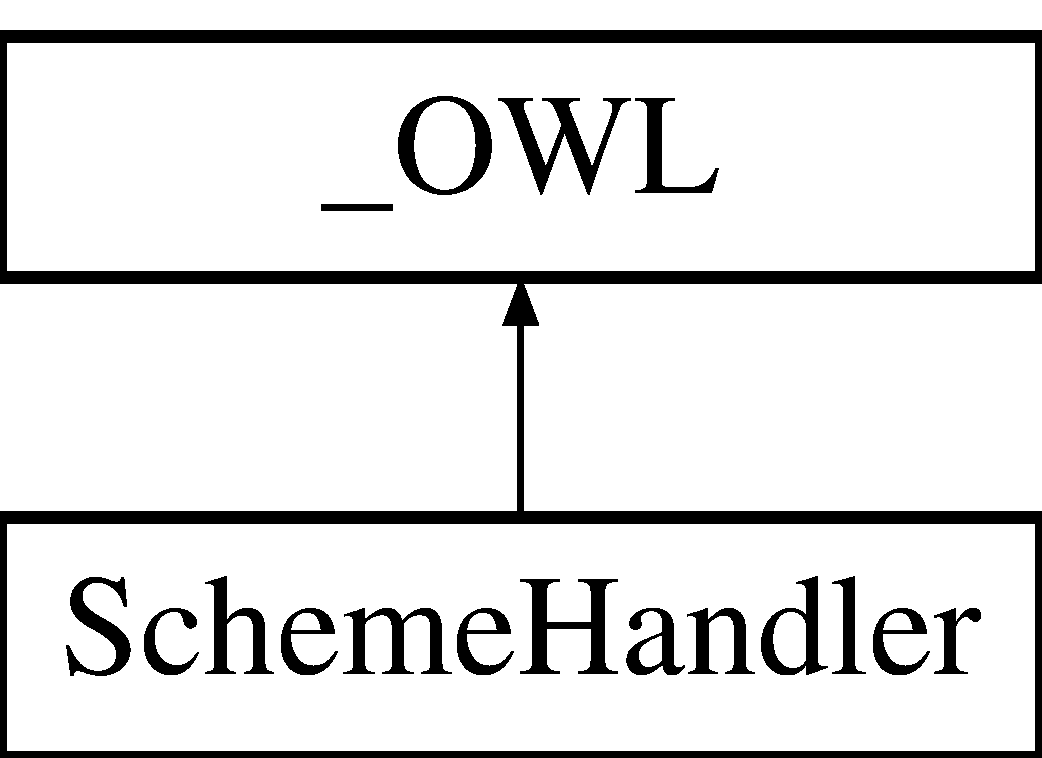
\includegraphics[height=2.000000cm]{classSchemeHandler}
\end{center}
\end{figure}
\subsection*{Public Member Functions}
\begin{DoxyCompactItemize}
\item 
{\bf \_\-\_\-destruct} ()
\item 
{\bf \_\-\_\-clone} ()
\item 
{\bf createScheme} (\$\_\-tblname)
\item 
{\bf defineScheme} (\$\_\-scheme)
\item 
{\bf defineIndex} (\$\_\-index)
\item 
{\bf scheme} (\$\_\-drops=false)
\item 
{\bf alterScheme} (\$\_\-field)
\item 
{\bf tableDescription} (\$tablename, \&\$data)
\item 
{\bf reset} ()
\item 
{\bf getLastWarning} ()
\item 
{\bf getStatus} ()
\item 
{\bf getSeverity} (\$status=null)
\item 
{\bf succeeded} (\$\_\-ok={\bf OWL\_\-SUCCESS}, \&\$\_\-object=null)
\item 
{\bf signal} (\$level={\bf OWL\_\-INFO}, \&\$text=false)
\item 
{\bf traceback} (\&\$text=false, \$depth=0)
\end{DoxyCompactItemize}
\subsection*{Static Public Member Functions}
\begin{DoxyCompactItemize}
\item 
static {\bf getInstance} ()
\end{DoxyCompactItemize}
\subsection*{Protected Member Functions}
\begin{DoxyCompactItemize}
\item 
{\bf init} ()
\item 
{\bf setCallback} (\$\_\-dispatcher)
\item 
{\bf setCallbackArgument} (array \$\_\-arg)
\item 
{\bf getCallback} ()
\item 
{\bf saveStatus} ()
\item 
{\bf restoreStatus} ()
\item 
{\bf check} (\&\$object, \$level={\bf OWL\_\-WARNING})
\item 
{\bf setStatus} (\$status, \$params=array())
\item 
{\bf setHighSeverity} (\&\$object=null)
\item 
{\bf stackMessage} (\$level={\bf OWL\_\-WARNING})
\end{DoxyCompactItemize}
\subsection*{Protected Attributes}
\begin{DoxyCompactItemize}
\item 
{\bf \$severity}
\end{DoxyCompactItemize}
\subsection*{Private Member Functions}
\begin{DoxyCompactItemize}
\item 
{\bf \_\-\_\-construct} ()
\item 
{\bf validateScheme} ()
\item 
{\bf compare} ()
\item 
{\bf createTable} ()
\item 
{\bf alterTable} (\$\_\-diffs, \$\_\-drops)
\item 
{\bf \_\-define\_\-field} (\$\_\-desc)
\item 
{\bf getTableColumns} (\$\_\-tablename)
\item 
{\bf getTableIndexes} (\$\_\-tablename)
\end{DoxyCompactItemize}
\subsection*{Private Attributes}
\begin{DoxyCompactItemize}
\item 
{\bf \$id}
\item 
{\bf \$db}
\item 
{\bf \$scheme}
\item 
{\bf \$table} = ''
\item 
{\bf \$inuse} = false
\end{DoxyCompactItemize}
\subsection*{Static Private Attributes}
\begin{DoxyCompactItemize}
\item 
static {\bf \$instance}
\end{DoxyCompactItemize}


\subsection{Detailed Description}
Scheme handler. 

Handler for all database schemes. This singleton class handles all updates to db tables \begin{DoxyAuthor}{Author}
Oscar van Eijk, Oveas Functionality Provider 
\end{DoxyAuthor}
\begin{DoxyVersion}{Version}
Oct 7, 2010 -\/-\/ O van Eijk -\/-\/ initial version for \doxyref{OWL}{p.}{classOWL} 
\end{DoxyVersion}
\begin{DoxyNote}{Note}
A port of this class has been created for VirtueMart 
\end{DoxyNote}
\begin{Desc}
\item[{\bf Todo}]This handler currently doesn't use the \doxyref{DbDriver}{p.}{interfaceDbDriver} driver class \end{Desc}


\subsection{Constructor \& Destructor Documentation}
\index{SchemeHandler@{SchemeHandler}!\_\-\_\-construct@{\_\-\_\-construct}}
\index{\_\-\_\-construct@{\_\-\_\-construct}!SchemeHandler@{SchemeHandler}}
\subsubsection[{\_\-\_\-construct}]{\setlength{\rightskip}{0pt plus 5cm}SchemeHandler::\_\-\_\-construct (
\begin{DoxyParamCaption}
{}
\end{DoxyParamCaption}
)\hspace{0.3cm}{\ttfamily  [private]}}\label{classSchemeHandler_ae528fde31fe73647c614ef6f957c4caf}
Class constructor \begin{DoxyAuthor}{Author}
Oscar van Eijk, Oveas Functionality Provider 
\end{DoxyAuthor}


References getInstance(), \_\-OWL::init(), and \_\-OWL::setStatus().

\index{SchemeHandler@{SchemeHandler}!\_\-\_\-destruct@{\_\-\_\-destruct}}
\index{\_\-\_\-destruct@{\_\-\_\-destruct}!SchemeHandler@{SchemeHandler}}
\subsubsection[{\_\-\_\-destruct}]{\setlength{\rightskip}{0pt plus 5cm}SchemeHandler::\_\-\_\-destruct (
\begin{DoxyParamCaption}
{}
\end{DoxyParamCaption}
)}\label{classSchemeHandler_a3d786efe6ef92858de21438b59774226}
Class destructor \begin{DoxyAuthor}{Author}
Oscar van Eijk, Oveas Functionality Provider 
\end{DoxyAuthor}


Reimplemented from {\bf \_\-OWL} \doxyref{}{p.}{class__OWL_a44fd2222476a3109286cc82d92b6bbcc}.



\subsection{Member Function Documentation}
\index{SchemeHandler@{SchemeHandler}!\_\-\_\-clone@{\_\-\_\-clone}}
\index{\_\-\_\-clone@{\_\-\_\-clone}!SchemeHandler@{SchemeHandler}}
\subsubsection[{\_\-\_\-clone}]{\setlength{\rightskip}{0pt plus 5cm}SchemeHandler::\_\-\_\-clone (
\begin{DoxyParamCaption}
{}
\end{DoxyParamCaption}
)}\label{classSchemeHandler_af0a48894ea6bb36f3149ccd40bf37681}
Implementation of the \doxyref{\_\-\_\-clone()}{p.}{classSchemeHandler_af0a48894ea6bb36f3149ccd40bf37681} function to prevent cloning of this singleton; it triggers a fatal (user)error \begin{DoxyAuthor}{Author}
Oscar van Eijk, Oveas Functionality Provider 
\end{DoxyAuthor}
\index{SchemeHandler@{SchemeHandler}!\_\-define\_\-field@{\_\-define\_\-field}}
\index{\_\-define\_\-field@{\_\-define\_\-field}!SchemeHandler@{SchemeHandler}}
\subsubsection[{\_\-define\_\-field}]{\setlength{\rightskip}{0pt plus 5cm}SchemeHandler::\_\-define\_\-field (
\begin{DoxyParamCaption}
\item[{\$}]{\_\-desc}
\end{DoxyParamCaption}
)\hspace{0.3cm}{\ttfamily  [private]}}\label{classSchemeHandler_a223d509509598fbc99741e910bda8cac}
Create the SQL code for a field definition 
\begin{DoxyParams}[1]{Parameters}
\mbox{\tt in}  & {\em \$\_\-desc} & Indexed array with the field properties from scheme definition \\
\hline
\end{DoxyParams}
\begin{DoxyReturn}{Returns}
string SQL code 
\end{DoxyReturn}
\begin{DoxyAuthor}{Author}
Oscar van Eijk, Oveas Functionality Provider 
\end{DoxyAuthor}


Referenced by alterTable(), and createTable().

\index{SchemeHandler@{SchemeHandler}!alterScheme@{alterScheme}}
\index{alterScheme@{alterScheme}!SchemeHandler@{SchemeHandler}}
\subsubsection[{alterScheme}]{\setlength{\rightskip}{0pt plus 5cm}SchemeHandler::alterScheme (
\begin{DoxyParamCaption}
\item[{\$}]{\_\-field}
\end{DoxyParamCaption}
)}\label{classSchemeHandler_a4072b1c3c04e4915cbd0e8926a8efb7a}
Modify 1 or more fields in an existing scheme definition 
\begin{DoxyParams}[1]{Parameters}
\mbox{\tt in}  & {\em \$\_\-field} & Array holding 1 or more field descriptions \\
\hline
\end{DoxyParams}
\begin{DoxySeeAlso}{See also}
\doxyref{defineScheme()}{p.}{classSchemeHandler_acadaf57e5f374f300501153056f227c5} 
\end{DoxySeeAlso}
\begin{DoxyReturn}{Returns}
Boolean; false if the table description contains errors 
\end{DoxyReturn}
\begin{DoxyAuthor}{Author}
Oscar van Eijk, Oveas Functionality Provider 
\end{DoxyAuthor}


References scheme(), \_\-OWL::setStatus(), and validateScheme().

\index{SchemeHandler@{SchemeHandler}!alterTable@{alterTable}}
\index{alterTable@{alterTable}!SchemeHandler@{SchemeHandler}}
\subsubsection[{alterTable}]{\setlength{\rightskip}{0pt plus 5cm}SchemeHandler::alterTable (
\begin{DoxyParamCaption}
\item[{\$}]{\_\-diffs, }
\item[{\$}]{\_\-drops}
\end{DoxyParamCaption}
)\hspace{0.3cm}{\ttfamily  [private]}}\label{classSchemeHandler_a498dc3fc0d51998422623ca64c84c52b}
Make changes to the table 
\begin{DoxyParams}[1]{Parameters}
\mbox{\tt in}  & {\em \$\_\-diffs} & Changes to make \\
\hline
\mbox{\tt in}  & {\em \$\_\-drops} & True if existing fields should be dropped \\
\hline
\end{DoxyParams}
\begin{DoxyAuthor}{Author}
Oscar van Eijk, Oveas Functionality Provider 
\end{DoxyAuthor}


References \_\-define\_\-field().



Referenced by scheme().

\index{SchemeHandler@{SchemeHandler}!check@{check}}
\index{check@{check}!SchemeHandler@{SchemeHandler}}
\subsubsection[{check}]{\setlength{\rightskip}{0pt plus 5cm}\_\-OWL::check (
\begin{DoxyParamCaption}
\item[{\&\$}]{object, }
\item[{\$}]{level = {\ttfamily {\bf OWL\_\-WARNING}}}
\end{DoxyParamCaption}
)\hspace{0.3cm}{\ttfamily  [protected, inherited]}}\label{class__OWL_ae2e3c56e5f3c4ce4156c6b1bb1c50f63}
This is a helper function for lazy developers. Some checks have to be made quite often, this is a kinda macro to handle that. It compares the own severity level with that of a given object. If the highest level is above a given max, a traceback and reset are performed.


\begin{DoxyParams}[1]{Parameters}
\mbox{\tt in}  & {\em \$object} & Pointer to an object to check against \\
\hline
\mbox{\tt in}  & {\em \$level} & The maximum severity level \\
\hline
\end{DoxyParams}
\begin{DoxyReturn}{Returns}
True if the severity level was correct (below the max), otherwise false 
\end{DoxyReturn}
\begin{DoxyAuthor}{Author}
Oscar van Eijk, Oveas Functionality Provider 
\end{DoxyAuthor}


References \_\-OWL::reset(), \_\-OWL::setHighSeverity(), and \_\-OWL::traceback().



Referenced by SessionHandler::write().

\index{SchemeHandler@{SchemeHandler}!compare@{compare}}
\index{compare@{compare}!SchemeHandler@{SchemeHandler}}
\subsubsection[{compare}]{\setlength{\rightskip}{0pt plus 5cm}SchemeHandler::compare (
\begin{DoxyParamCaption}
{}
\end{DoxyParamCaption}
)\hspace{0.3cm}{\ttfamily  [private]}}\label{classSchemeHandler_ae2a981feae465ef5e46782b4a18da1ad}
Compare the scheme with an existing database table \begin{DoxyReturn}{Returns}
mixed True if there are no differences, False if the table does not exist, or an array with differences 
\end{DoxyReturn}
\begin{DoxyAuthor}{Author}
Oscar van Eijk, Oveas Functionality Provider 
\end{DoxyAuthor}


References \_\-OWL::getStatus(), scheme(), and tableDescription().



Referenced by scheme().

\index{SchemeHandler@{SchemeHandler}!createScheme@{createScheme}}
\index{createScheme@{createScheme}!SchemeHandler@{SchemeHandler}}
\subsubsection[{createScheme}]{\setlength{\rightskip}{0pt plus 5cm}SchemeHandler::createScheme (
\begin{DoxyParamCaption}
\item[{\$}]{\_\-tblname}
\end{DoxyParamCaption}
)}\label{classSchemeHandler_a49bc2a5dd43188f83824aafd9fbff9eb}
Set a new tablename 
\begin{DoxyParams}[1]{Parameters}
\mbox{\tt in}  & {\em \$\_\-tblname} & Name of the table to create, check or modify \\
\hline
\end{DoxyParams}
\begin{DoxyAuthor}{Author}
Oscar van Eijk, Oveas Functionality Provider 
\end{DoxyAuthor}


References reset(), and \_\-OWL::setStatus().

\index{SchemeHandler@{SchemeHandler}!createTable@{createTable}}
\index{createTable@{createTable}!SchemeHandler@{SchemeHandler}}
\subsubsection[{createTable}]{\setlength{\rightskip}{0pt plus 5cm}SchemeHandler::createTable (
\begin{DoxyParamCaption}
{}
\end{DoxyParamCaption}
)\hspace{0.3cm}{\ttfamily  [private]}}\label{classSchemeHandler_a7c5939939cb2ba71ed5a32bc987f0c71}
Create the defined table \begin{DoxyAuthor}{Author}
Oscar van Eijk, Oveas Functionality Provider 
\end{DoxyAuthor}


References \_\-define\_\-field(), and scheme().



Referenced by scheme().

\index{SchemeHandler@{SchemeHandler}!defineIndex@{defineIndex}}
\index{defineIndex@{defineIndex}!SchemeHandler@{SchemeHandler}}
\subsubsection[{defineIndex}]{\setlength{\rightskip}{0pt plus 5cm}SchemeHandler::defineIndex (
\begin{DoxyParamCaption}
\item[{\$}]{\_\-index}
\end{DoxyParamCaption}
)}\label{classSchemeHandler_abc00b9ccfdf0681a3e5d333ad11db0e1}
Define the indexes for a table 
\begin{DoxyParams}[1]{Parameters}
\mbox{\tt in}  & {\em \$\_\-index} & Array holding the index description. This is a 2 dimensional array where the first level holds the indexname. The second array defines the attributes for each index:
\begin{DoxyItemize}
\item unique : Boolean; True for unique keys
\item primary : Boolean; True for the primary key
\item columns : Array; List with columnnames that will be indexed
\item type : String (optional); Index type, currenty only supports 'FULLTEXT' 
\end{DoxyItemize}\\
\hline
\end{DoxyParams}
\begin{DoxyReturn}{Returns}
Severity level 
\end{DoxyReturn}
\begin{DoxyAuthor}{Author}
Oscar van Eijk, Oveas Functionality Provider 
\end{DoxyAuthor}


References scheme(), \_\-OWL::setStatus(), and validateScheme().

\index{SchemeHandler@{SchemeHandler}!defineScheme@{defineScheme}}
\index{defineScheme@{defineScheme}!SchemeHandler@{SchemeHandler}}
\subsubsection[{defineScheme}]{\setlength{\rightskip}{0pt plus 5cm}SchemeHandler::defineScheme (
\begin{DoxyParamCaption}
\item[{\$}]{\_\-scheme}
\end{DoxyParamCaption}
)}\label{classSchemeHandler_acadaf57e5f374f300501153056f227c5}
Define the layout for a table 
\begin{DoxyParams}[1]{Parameters}
\mbox{\tt in}  & {\em \$\_\-scheme} & Array holding the table description. This is a 2 dimensional array where the first level holds the fieldnames. The second array defines the attributes for each field:
\begin{DoxyItemize}
\item type : String; the field-\/type (INT$|$TINYINT$|$VARCHAR$|$MEDIUMTEXT$|$TEXT$|$LONGTEXT$|$BLOB$|$LONGBLOB$|$ENUM$|$SET)
\item length : Integer; indicating the length for fieldtypes that use that (like INT and VARCHAR)
\item null : Boolean; when true the value can be NULL
\item auto-\/inc : Boolean; True for auto-\/increment values (will be set as primary key)
\item default : Mixed; default value
\item options : Array; for SET and ENUM types. the list of possible values
\item comment : String; field comment 
\end{DoxyItemize}\\
\hline
\end{DoxyParams}
\begin{DoxyAuthor}{Author}
Oscar van Eijk, Oveas Functionality Provider 
\end{DoxyAuthor}


References scheme(), \_\-OWL::setStatus(), and validateScheme().

\index{SchemeHandler@{SchemeHandler}!getCallback@{getCallback}}
\index{getCallback@{getCallback}!SchemeHandler@{SchemeHandler}}
\subsubsection[{getCallback}]{\setlength{\rightskip}{0pt plus 5cm}\_\-OWL::getCallback (
\begin{DoxyParamCaption}
{}
\end{DoxyParamCaption}
)\hspace{0.3cm}{\ttfamily  [protected, inherited]}}\label{class__OWL_acb46ff88f43ca66f1268d3f5199c3f8d}
Retrieve a previously set (callback) dispatcher. The (callback) dispatcher is cleared immediatly. \begin{DoxyReturn}{Returns}
The dispatcher, of null on failure. 
\end{DoxyReturn}
\begin{DoxyAuthor}{Author}
Oscar van Eijk, Oveas Functionality Provider 
\end{DoxyAuthor}


Reimplemented in {\bf Dispatcher} \doxyref{}{p.}{classDispatcher_a31c4bd4e4eaee7ef90b1ea364a901447}.



References OWL::factory().

\index{SchemeHandler@{SchemeHandler}!getInstance@{getInstance}}
\index{getInstance@{getInstance}!SchemeHandler@{SchemeHandler}}
\subsubsection[{getInstance}]{\setlength{\rightskip}{0pt plus 5cm}static SchemeHandler::getInstance (
\begin{DoxyParamCaption}
{}
\end{DoxyParamCaption}
)\hspace{0.3cm}{\ttfamily  [static]}}\label{classSchemeHandler_aedfe445dbf679209066213b64d883c7d}
Return a reference to my implementation. If necessary, create that implementation first. \begin{DoxyReturn}{Returns}
Severity level 
\end{DoxyReturn}
\begin{DoxyAuthor}{Author}
Oscar van Eijk, Oveas Functionality Provider 
\end{DoxyAuthor}


References \$instance.



Referenced by \_\-\_\-construct().

\index{SchemeHandler@{SchemeHandler}!getLastWarning@{getLastWarning}}
\index{getLastWarning@{getLastWarning}!SchemeHandler@{SchemeHandler}}
\subsubsection[{getLastWarning}]{\setlength{\rightskip}{0pt plus 5cm}\_\-OWL::getLastWarning (
\begin{DoxyParamCaption}
{}
\end{DoxyParamCaption}
)\hspace{0.3cm}{\ttfamily  [inherited]}}\label{class__OWL_a1888f52fc2d0ec29e146925ccad70a6b}
Get the last warning or error message. \begin{DoxyReturn}{Returns}
null if there was no error (severity below OWL\_\-WARNING), otherwise the error text. 
\end{DoxyReturn}
\begin{DoxyAuthor}{Author}
Oscar van Eijk, Oveas Functionality Provider 
\end{DoxyAuthor}


References \_\-OWL::signal().

\index{SchemeHandler@{SchemeHandler}!getSeverity@{getSeverity}}
\index{getSeverity@{getSeverity}!SchemeHandler@{SchemeHandler}}
\subsubsection[{getSeverity}]{\setlength{\rightskip}{0pt plus 5cm}\_\-OWL::getSeverity (
\begin{DoxyParamCaption}
\item[{\$}]{status = {\ttfamily null}}
\end{DoxyParamCaption}
)\hspace{0.3cm}{\ttfamily  [inherited]}}\label{class__OWL_a2374613f9bb7eccf49a5dbc9a9ef4751}
Get the current object severity level. 
\begin{DoxyParams}[1]{Parameters}
\mbox{\tt in}  & {\em \$status} & An optional parameter to check an other status code i.s.o the object's current status. \\
\hline
\end{DoxyParams}
\begin{DoxyReturn}{Returns}
Status severity level 
\end{DoxyReturn}
\begin{DoxyAuthor}{Author}
Oscar van Eijk, Oveas Functionality Provider 
\end{DoxyAuthor}


References \_\-OWL::\$status.



Referenced by LogHandler::composeMessage(), LogHandler::log(), and DataHandler::setKey().

\index{SchemeHandler@{SchemeHandler}!getStatus@{getStatus}}
\index{getStatus@{getStatus}!SchemeHandler@{SchemeHandler}}
\subsubsection[{getStatus}]{\setlength{\rightskip}{0pt plus 5cm}\_\-OWL::getStatus (
\begin{DoxyParamCaption}
{}
\end{DoxyParamCaption}
)\hspace{0.3cm}{\ttfamily  [final, inherited]}}\label{class__OWL_ac1f1643ff5b5db7c326c30477603358d}
Get the current object status. \begin{DoxyReturn}{Returns}
Object's status code 
\end{DoxyReturn}
\begin{DoxyAuthor}{Author}
Oscar van Eijk, Oveas Functionality Provider 
\end{DoxyAuthor}


Referenced by compare().

\index{SchemeHandler@{SchemeHandler}!getTableColumns@{getTableColumns}}
\index{getTableColumns@{getTableColumns}!SchemeHandler@{SchemeHandler}}
\subsubsection[{getTableColumns}]{\setlength{\rightskip}{0pt plus 5cm}SchemeHandler::getTableColumns (
\begin{DoxyParamCaption}
\item[{\$}]{\_\-tablename}
\end{DoxyParamCaption}
)\hspace{0.3cm}{\ttfamily  [private]}}\label{classSchemeHandler_abbf0ce7a23293498c32227e2554ce849}
Get the columns for a given table 
\begin{DoxyParams}[1]{Parameters}
\mbox{\tt in}  & {\em \$\_\-tablename} & The tablename \\
\hline
\end{DoxyParams}
\begin{DoxyReturn}{Returns}
Indexed array holding all fields =$>$ datatypes, or null on errors 
\end{DoxyReturn}
\begin{DoxyAuthor}{Author}
Oscar van Eijk, Oveas Functionality Provider 
\end{DoxyAuthor}


References \_\-OWL::setStatus().



Referenced by tableDescription().

\index{SchemeHandler@{SchemeHandler}!getTableIndexes@{getTableIndexes}}
\index{getTableIndexes@{getTableIndexes}!SchemeHandler@{SchemeHandler}}
\subsubsection[{getTableIndexes}]{\setlength{\rightskip}{0pt plus 5cm}SchemeHandler::getTableIndexes (
\begin{DoxyParamCaption}
\item[{\$}]{\_\-tablename}
\end{DoxyParamCaption}
)\hspace{0.3cm}{\ttfamily  [private]}}\label{classSchemeHandler_af40c242f4bddee235dbce50a7535b094}
Get the indexes for a given table 
\begin{DoxyParams}[1]{Parameters}
\mbox{\tt in}  & {\em \$\_\-tablename} & The tablename \\
\hline
\end{DoxyParams}
\begin{DoxyReturn}{Returns}
Indexed array holding all fields =$>$ datatypes, or null on errors 
\end{DoxyReturn}
\begin{DoxyAuthor}{Author}
Oscar van Eijk, Oveas Functionality Provider 
\end{DoxyAuthor}


References \_\-OWL::setStatus().



Referenced by tableDescription().

\index{SchemeHandler@{SchemeHandler}!init@{init}}
\index{init@{init}!SchemeHandler@{SchemeHandler}}
\subsubsection[{init}]{\setlength{\rightskip}{0pt plus 5cm}\_\-OWL::init (
\begin{DoxyParamCaption}
{}
\end{DoxyParamCaption}
)\hspace{0.3cm}{\ttfamily  [protected, inherited]}}\label{class__OWL_ae0ef3ded56e8a6b34b6461e5a721cd3e}
This function should be called by all constuctors. It initializes the general characteristics. Status is 'warning' by default, it's up to the contructor to set a proper status; if it's still 'warning', this $\ast$might$\ast$ indicate something went wrong. \begin{DoxyAuthor}{Author}
Oscar van Eijk, Oveas Functionality Provider 
\end{DoxyAuthor}


References OWL::factory(), and \_\-OWL::setStatus().



Referenced by FormFieldPlugin::\_\-\_\-construct(), Document::\_\-\_\-construct(), ContainerPlugin::\_\-\_\-construct(), Container::\_\-\_\-construct(), SocketHandler::\_\-\_\-construct(), SessionHandler::\_\-\_\-construct(), \_\-\_\-construct(), LogHandler::\_\-\_\-construct(), ImageHandler::\_\-\_\-construct(), FormHandler::\_\-\_\-construct(), FileHandler::\_\-\_\-construct(), DbHandler::\_\-\_\-construct(), HDataHandler::\_\-\_\-construct(), DataHandler::\_\-\_\-construct(), OWL::\_\-\_\-construct(), Mail::\_\-\_\-construct(), Group::\_\-\_\-construct(), Form::\_\-\_\-construct(), Dispatcher::\_\-\_\-construct(), and User::construct().

\index{SchemeHandler@{SchemeHandler}!reset@{reset}}
\index{reset@{reset}!SchemeHandler@{SchemeHandler}}
\subsubsection[{reset}]{\setlength{\rightskip}{0pt plus 5cm}SchemeHandler::reset (
\begin{DoxyParamCaption}
{}
\end{DoxyParamCaption}
)}\label{classSchemeHandler_aa25feb4a70d67b3d571904be4b2f50bc}
Reset the internal data structure \begin{DoxyAuthor}{Author}
Oscar van Eijk, Oveas Functionality Provider 
\end{DoxyAuthor}


Reimplemented from {\bf \_\-OWL} \doxyref{}{p.}{class__OWL_a2f2a042bcf31965194c03033df0edc9b}.



References scheme().



Referenced by createScheme().

\index{SchemeHandler@{SchemeHandler}!restoreStatus@{restoreStatus}}
\index{restoreStatus@{restoreStatus}!SchemeHandler@{SchemeHandler}}
\subsubsection[{restoreStatus}]{\setlength{\rightskip}{0pt plus 5cm}\_\-OWL::restoreStatus (
\begin{DoxyParamCaption}
{}
\end{DoxyParamCaption}
)\hspace{0.3cm}{\ttfamily  [protected, inherited]}}\label{class__OWL_a93de01a9bbbc3f228e1a62a0740e90f0}
Restore the previously saved status object and destroy the copy \begin{DoxyAuthor}{Author}
Oscar van Eijk, Oveas Functionality Provider 
\end{DoxyAuthor}


References \_\-OWL::setStatus().



Referenced by User::logout().

\index{SchemeHandler@{SchemeHandler}!saveStatus@{saveStatus}}
\index{saveStatus@{saveStatus}!SchemeHandler@{SchemeHandler}}
\subsubsection[{saveStatus}]{\setlength{\rightskip}{0pt plus 5cm}\_\-OWL::saveStatus (
\begin{DoxyParamCaption}
{}
\end{DoxyParamCaption}
)\hspace{0.3cm}{\ttfamily  [protected, inherited]}}\label{class__OWL_add923dc756471318edca8883db3f4420}
Create a copy of the status object \begin{DoxyAuthor}{Author}
Oscar van Eijk, Oveas Functionality Provider 
\end{DoxyAuthor}


Referenced by User::logout().

\index{SchemeHandler@{SchemeHandler}!scheme@{scheme}}
\index{scheme@{scheme}!SchemeHandler@{SchemeHandler}}
\subsubsection[{scheme}]{\setlength{\rightskip}{0pt plus 5cm}SchemeHandler::scheme (
\begin{DoxyParamCaption}
\item[{\$}]{\_\-drops = {\ttfamily false}}
\end{DoxyParamCaption}
)}\label{classSchemeHandler_a1e843dc411d175818c7b2ab5374f021e}
If the table does not exist, or differs from the defined scheme, create of modify the table 
\begin{DoxyParams}[1]{Parameters}
\mbox{\tt in}  & {\em \$\_\-drops} & True if existing fields should be dropped; default false. If existing fields should be converted to new fields, call with DbScheme::scheme(false) first, then do the conversions, next call DbScheme::scheme(true). \\
\hline
\end{DoxyParams}
\begin{DoxyReturn}{Returns}
Severity level 
\end{DoxyReturn}
\begin{DoxyAuthor}{Author}
Oscar van Eijk, Oveas Functionality Provider 
\end{DoxyAuthor}


References alterTable(), compare(), createTable(), and \_\-OWL::setStatus().



Referenced by alterScheme(), compare(), createTable(), defineIndex(), defineScheme(), reset(), and validateScheme().

\index{SchemeHandler@{SchemeHandler}!setCallback@{setCallback}}
\index{setCallback@{setCallback}!SchemeHandler@{SchemeHandler}}
\subsubsection[{setCallback}]{\setlength{\rightskip}{0pt plus 5cm}\_\-OWL::setCallback (
\begin{DoxyParamCaption}
\item[{\$}]{\_\-dispatcher}
\end{DoxyParamCaption}
)\hspace{0.3cm}{\ttfamily  [protected, inherited]}}\label{class__OWL_a5f84d43cd4dc7810649f1e2ebecad360}
Set a dispatcher for later callback 
\begin{DoxyParams}[1]{Parameters}
\mbox{\tt in}  & {\em \$\_\-dispatcher} & Dispatched, \\
\hline
\end{DoxyParams}
\begin{DoxySeeAlso}{See also}
\doxyref{Dispatcher::composeDispatcher()}{p.}{classDispatcher_a8a974bbbb30be7cda74f9929972fd2f6} 
\end{DoxySeeAlso}
\begin{DoxyReturn}{Returns}
True on success, false on failure 
\end{DoxyReturn}
\begin{DoxyAuthor}{Author}
Oscar van Eijk, Oveas Functionality Provider 
\end{DoxyAuthor}


References OWL::factory().

\index{SchemeHandler@{SchemeHandler}!setCallbackArgument@{setCallbackArgument}}
\index{setCallbackArgument@{setCallbackArgument}!SchemeHandler@{SchemeHandler}}
\subsubsection[{setCallbackArgument}]{\setlength{\rightskip}{0pt plus 5cm}\_\-OWL::setCallbackArgument (
\begin{DoxyParamCaption}
\item[{array \$}]{\_\-arg}
\end{DoxyParamCaption}
)\hspace{0.3cm}{\ttfamily  [protected, inherited]}}\label{class__OWL_a4e9ebfbd3c0d76539bed4e44de9962c3}
Add an argument to a previously registered callback dispatcher 
\begin{DoxyParams}[1]{Parameters}
\mbox{\tt in}  & {\em \$\_\-arg} & Argument, must be an array type. When non-\/ arrays should be passed as arguments, the must be set when the callback is registered already \\
\hline
\end{DoxyParams}
\begin{DoxyReturn}{Returns}
True on success, false on failure 
\end{DoxyReturn}
\begin{DoxyAuthor}{Author}
Oscar van Eijk, Oveas Functionality Provider 
\end{DoxyAuthor}


References OWL::factory().



Referenced by User::register().

\index{SchemeHandler@{SchemeHandler}!setHighSeverity@{setHighSeverity}}
\index{setHighSeverity@{setHighSeverity}!SchemeHandler@{SchemeHandler}}
\subsubsection[{setHighSeverity}]{\setlength{\rightskip}{0pt plus 5cm}\_\-OWL::setHighSeverity (
\begin{DoxyParamCaption}
\item[{\&\$}]{object = {\ttfamily null}}
\end{DoxyParamCaption}
)\hspace{0.3cm}{\ttfamily  [protected, inherited]}}\label{class__OWL_a97173dbe452428d3851406413264734d}
Compare the severity level of the current object with a given one and set my statuspointer to the object with the highest level. \begin{DoxyAuthor}{Author}
Oscar van Eijk, Oveas Functionality Provider 
\end{DoxyAuthor}


Referenced by \_\-OWL::check(), DataHandler::db(), DataHandler::prepare(), and SessionHandler::read().

\index{SchemeHandler@{SchemeHandler}!setStatus@{setStatus}}
\index{setStatus@{setStatus}!SchemeHandler@{SchemeHandler}}
\subsubsection[{setStatus}]{\setlength{\rightskip}{0pt plus 5cm}\_\-OWL::setStatus (
\begin{DoxyParamCaption}
\item[{\$}]{status, }
\item[{\$}]{params = {\ttfamily array~()}}
\end{DoxyParamCaption}
)\hspace{0.3cm}{\ttfamily  [final, protected, inherited]}}\label{class__OWL_a80e2fe01c3663dbb0ab685eebe33fd1e}
Set the current object status to the specified value. 
\begin{DoxyParams}[1]{Parameters}
\mbox{\tt in}  & {\em \$status} & \doxyref{OWL}{p.}{classOWL} status code \\
\hline
\mbox{\tt in}  & {\em \$params} & \\
\hline
\end{DoxyParams}
\begin{DoxyAuthor}{Author}
Oscar van Eijk, Oveas Functionality Provider 
\end{DoxyAuthor}


References \$GLOBALS, \_\-OWL::\$status, ConfigHandler::get(), Register::getCode(), \_\-OWL::reset(), and \_\-OWL::signal().



Referenced by DbHandler::\_\-\_\-clone(), Container::\_\-\_\-construct(), SocketHandler::\_\-\_\-construct(), \_\-\_\-construct(), ImageHandler::\_\-\_\-construct(), FormHandler::\_\-\_\-construct(), FileHandler::\_\-\_\-construct(), DbHandler::\_\-\_\-construct(), DataHandler::\_\-\_\-construct(), Session::\_\-\_\-construct(), Mail::\_\-\_\-construct(), BaseElement::\_\-getContent(), HDataHandler::\_\-getNewLeft(), Mail::addBcc(), Mail::addCc(), Container::addContainer(), Form::addField(), FormFieldRadioPlugin::addOption(), HDataHandler::addParent(), Mail::addTo(), BaseElement::addToContent(), DbHandler::alt(), alterScheme(), FileHandler::close(), DbHandler::commitTransaction(), Dispatcher::composeDispatcher(), User::confirm(), SocketHandler::connect(), DbHandler::connect(), DbHandler::create(), createScheme(), DbHandler::dbread(), defineIndex(), defineScheme(), SocketHandler::disconnect(), Dispatcher::dispatch(), HDataHandler::enableCrossLink(), FormHandler::get(), DataHandler::get(), HDataHandler::getDirectChildren(), HDataHandler::getFullOffspring(), Group::getGroupByName(), getTableColumns(), getTableIndexes(), \_\-OWL::init(), Document::loadScript(), Document::loadStyle(), DbHandler::lockTable(), User::login(), HDataHandler::moveNode(), FileHandler::open(), DbHandler::open(), LogHandler::openLogfile(), DataHandler::prepare(), DbHandler::prepareDelete(), DbHandler::prepareField(), DbHandler::prepareInsert(), DbHandler::prepareRead(), DbHandler::prepareUpdate(), SocketHandler::read(), DbHandler::read(), FileHandler::readLine(), HDataHandler::readQuery(), User::readUserdata(), User::register(), Dispatcher::registerArgument(), Dispatcher::registerCallback(), DbHandler::resetTable(), \_\-OWL::restoreStatus(), DbHandler::rollbackTransaction(), scheme(), Mail::send(), FormHandler::set(), BaseElement::setAttributes(), BaseElement::setContent(), Form::setEncoding(), Document::setFavicon(), Form::setFieldAttributes(), Mail::setFrom(), DataHandler::setJoin(), DataHandler::setKey(), FormFieldTextPlugin::setMaxsize(), Document::setMeta(), Form::setMethod(), FormFieldRadioPlugin::setSelected(), Mail::setSender(), FormFieldTextPlugin::setSize(), FormFieldSelectPlugin::setSize(), FormFieldSelectPlugin::setValue(), Form::showField(), DbHandler::startTransaction(), tableDescription(), DbHandler::unlockTable(), validateScheme(), SocketHandler::write(), DbHandler::write(), and HDataHandler::writeQuery().

\index{SchemeHandler@{SchemeHandler}!signal@{signal}}
\index{signal@{signal}!SchemeHandler@{SchemeHandler}}
\subsubsection[{signal}]{\setlength{\rightskip}{0pt plus 5cm}\_\-OWL::signal (
\begin{DoxyParamCaption}
\item[{\$}]{level = {\ttfamily {\bf OWL\_\-INFO}}, }
\item[{\&\$}]{text = {\ttfamily false}}
\end{DoxyParamCaption}
)\hspace{0.3cm}{\ttfamily  [inherited]}}\label{class__OWL_a51ba4a16409acf2a2f61f286939091a5}
Display the message for the current object status 
\begin{DoxyParams}[1]{Parameters}
\mbox{\tt in}  & {\em \$level} & An optional severity level; message will only be displayed when it is at least of this level. \\
\hline
\mbox{\tt out}  & {\em \$text} & If this parameter is given, the message text is returned in this string instead of echood. \\
\hline
\end{DoxyParams}
\begin{DoxyReturn}{Returns}
The severity level for this object 
\end{DoxyReturn}
\begin{DoxyAuthor}{Author}
Oscar van Eijk, Oveas Functionality Provider 
\end{DoxyAuthor}


References ConfigHandler::get(), OutputHandler::outputLine(), and OutputHandler::outputRaw().



Referenced by \_\-OWL::getLastWarning(), \_\-OWL::setStatus(), \_\-OWL::stackMessage(), and \_\-OWL::traceback().

\index{SchemeHandler@{SchemeHandler}!stackMessage@{stackMessage}}
\index{stackMessage@{stackMessage}!SchemeHandler@{SchemeHandler}}
\subsubsection[{stackMessage}]{\setlength{\rightskip}{0pt plus 5cm}\_\-OWL::stackMessage (
\begin{DoxyParamCaption}
\item[{\$}]{level = {\ttfamily {\bf OWL\_\-WARNING}}}
\end{DoxyParamCaption}
)\hspace{0.3cm}{\ttfamily  [protected, inherited]}}\label{class__OWL_acbb85f4949ca4bbd8bb2408362632cbc}
Add the message for the latests status change to the document \begin{DoxySeeAlso}{See also}
\doxyref{Document::addMessage()}{p.}{classDocument_aee4ecb0f14972dafd3114659b57048b3} 
\end{DoxySeeAlso}

\begin{DoxyParams}[1]{Parameters}
\mbox{\tt in}  & {\em \$level} & Minimum severity level \\
\hline
\end{DoxyParams}
\begin{DoxyAuthor}{Author}
Oscar van Eijk, Oveas Functionality Provider 
\end{DoxyAuthor}


References \$\_\-doc, \_\-OWL::\$severity, OWL::factory(), and \_\-OWL::signal().

\index{SchemeHandler@{SchemeHandler}!succeeded@{succeeded}}
\index{succeeded@{succeeded}!SchemeHandler@{SchemeHandler}}
\subsubsection[{succeeded}]{\setlength{\rightskip}{0pt plus 5cm}\_\-OWL::succeeded (
\begin{DoxyParamCaption}
\item[{\$}]{\_\-ok = {\ttfamily {\bf OWL\_\-SUCCESS}}, }
\item[{\&\$}]{\_\-object = {\ttfamily null}}
\end{DoxyParamCaption}
)\hspace{0.3cm}{\ttfamily  [inherited]}}\label{class__OWL_a53ab4d3bbb2c6a56966c339ca4b4c805}
Check if the object currenlty has a success state 
\begin{DoxyParams}[1]{Parameters}
\mbox{\tt in}  & {\em \$\_\-ok} & The highest severity that's considered successfull, default OWL\_\-SUCCESS \\
\hline
\mbox{\tt in}  & {\em \$\_\-object} & REference to the object to check, defaults to the current object \\
\hline
\end{DoxyParams}
\begin{DoxyReturn}{Returns}
Boolean true when successfull 
\end{DoxyReturn}
\begin{DoxyAuthor}{Author}
Oscar van Eijk, Oveas Functionality Provider 
\end{DoxyAuthor}


Referenced by User::construct(), Dispatcher::registerArgument(), and Dispatcher::registerCallback().

\index{SchemeHandler@{SchemeHandler}!tableDescription@{tableDescription}}
\index{tableDescription@{tableDescription}!SchemeHandler@{SchemeHandler}}
\subsubsection[{tableDescription}]{\setlength{\rightskip}{0pt plus 5cm}SchemeHandler::tableDescription (
\begin{DoxyParamCaption}
\item[{\$}]{tablename, }
\item[{\&\$}]{data}
\end{DoxyParamCaption}
)}\label{classSchemeHandler_a3ec1c9bb94164aa23faa06dea8fa187e}
Get a description of a database table 
\begin{DoxyParams}[1]{Parameters}
\mbox{\tt in}  & {\em \$tablename} & The tablename \\
\hline
\mbox{\tt out}  & {\em \$data} & Indexed array holding all fields =$>$ datatypes \\
\hline
\end{DoxyParams}
\begin{DoxyReturn}{Returns}
Severity level 
\end{DoxyReturn}
\begin{DoxyAuthor}{Author}
Oscar van Eijk, Oveas Functionality Provider 
\end{DoxyAuthor}


References getTableColumns(), getTableIndexes(), and \_\-OWL::setStatus().



Referenced by compare().

\index{SchemeHandler@{SchemeHandler}!traceback@{traceback}}
\index{traceback@{traceback}!SchemeHandler@{SchemeHandler}}
\subsubsection[{traceback}]{\setlength{\rightskip}{0pt plus 5cm}\_\-OWL::traceback (
\begin{DoxyParamCaption}
\item[{\&\$}]{text = {\ttfamily false}, }
\item[{\$}]{depth = {\ttfamily 0}}
\end{DoxyParamCaption}
)\hspace{0.3cm}{\ttfamily  [inherited]}}\label{class__OWL_aa29547995d6741b7d2b90c1d4ea99a13}
If somehwere in the nested calls an error occured, we can traceback the original failing object with this function and signal the message. 
\begin{DoxyParams}[1]{Parameters}
\mbox{\tt out}  & {\em \$text} & Optional variable in which the message text can be stored. If not given, the text will be written to standard output \\
\hline
\mbox{\tt in}  & {\em \$depth} & This paramater should be initially empty. It calculates the depth in recursive calls. \\
\hline
\end{DoxyParams}
\begin{DoxyReturn}{Returns}
Severity code of the failing object 
\end{DoxyReturn}
\begin{DoxyAuthor}{Author}
Oscar van Eijk, Oveas Functionality Provider 
\end{DoxyAuthor}


References \_\-OWL::signal().



Referenced by \_\-OWL::check(), User::login(), and SessionHandler::read().

\index{SchemeHandler@{SchemeHandler}!validateScheme@{validateScheme}}
\index{validateScheme@{validateScheme}!SchemeHandler@{SchemeHandler}}
\subsubsection[{validateScheme}]{\setlength{\rightskip}{0pt plus 5cm}SchemeHandler::validateScheme (
\begin{DoxyParamCaption}
{}
\end{DoxyParamCaption}
)\hspace{0.3cm}{\ttfamily  [private]}}\label{classSchemeHandler_addc471d7e188ad7131f69fd7adbd268b}
Validate the defined scheme. Some values will be modified to make sure the SQL statements can be prepared and \doxyref{compare()}{p.}{classSchemeHandler_ae2a981feae465ef5e46782b4a18da1ad} won't find differences on case diffs \begin{DoxyReturn}{Returns}
boolean False if there is an error in the scheme definition, True if no errors were found 
\end{DoxyReturn}
\begin{DoxyAuthor}{Author}
Oscar van Eijk, Oveas Functionality Provider 
\end{DoxyAuthor}


References scheme(), and \_\-OWL::setStatus().



Referenced by alterScheme(), defineIndex(), and defineScheme().



\subsection{Member Data Documentation}
\index{SchemeHandler@{SchemeHandler}!\$db@{\$db}}
\index{\$db@{\$db}!SchemeHandler@{SchemeHandler}}
\subsubsection[{\$db}]{\setlength{\rightskip}{0pt plus 5cm}SchemeHandler::\$db\hspace{0.3cm}{\ttfamily  [private]}}\label{classSchemeHandler_abf3bf26e35b759ccd49f358dedc2dfd1}
integer -\/ Reference to the database class \index{SchemeHandler@{SchemeHandler}!\$id@{\$id}}
\index{\$id@{\$id}!SchemeHandler@{SchemeHandler}}
\subsubsection[{\$id}]{\setlength{\rightskip}{0pt plus 5cm}SchemeHandler::\$id\hspace{0.3cm}{\ttfamily  [private]}}\label{classSchemeHandler_af297e966eae06ff1e38a143f93b4aeb9}
integer -\/ Scheme Handle ID \index{SchemeHandler@{SchemeHandler}!\$instance@{\$instance}}
\index{\$instance@{\$instance}!SchemeHandler@{SchemeHandler}}
\subsubsection[{\$instance}]{\setlength{\rightskip}{0pt plus 5cm}SchemeHandler::\$instance\hspace{0.3cm}{\ttfamily  [static, private]}}\label{classSchemeHandler_a6f45c52527230b3f3b60d75a9b55e3c1}
integer -\/ self reference 

Referenced by getInstance().

\index{SchemeHandler@{SchemeHandler}!\$inuse@{\$inuse}}
\index{\$inuse@{\$inuse}!SchemeHandler@{SchemeHandler}}
\subsubsection[{\$inuse}]{\setlength{\rightskip}{0pt plus 5cm}SchemeHandler::\$inuse = false\hspace{0.3cm}{\ttfamily  [private]}}\label{classSchemeHandler_a90e5b04603f86c04b1691b2ddf730104}
boolean -\/ True when a scheme is filled with data and not yet used \index{SchemeHandler@{SchemeHandler}!\$scheme@{\$scheme}}
\index{\$scheme@{\$scheme}!SchemeHandler@{SchemeHandler}}
\subsubsection[{\$scheme}]{\setlength{\rightskip}{0pt plus 5cm}SchemeHandler::\$scheme\hspace{0.3cm}{\ttfamily  [private]}}\label{classSchemeHandler_aeb6dfa54ebd11b0d6acc51b8244d598c}
Array -\/ table description \index{SchemeHandler@{SchemeHandler}!\$severity@{\$severity}}
\index{\$severity@{\$severity}!SchemeHandler@{SchemeHandler}}
\subsubsection[{\$severity}]{\setlength{\rightskip}{0pt plus 5cm}\_\-OWL::\$severity\hspace{0.3cm}{\ttfamily  [protected, inherited]}}\label{class__OWL_ad26b40a9dbbacb33e299b17826f8327c}
Severity level of the current object status 

Referenced by \_\-OWL::stackMessage().

\index{SchemeHandler@{SchemeHandler}!\$table@{\$table}}
\index{\$table@{\$table}!SchemeHandler@{SchemeHandler}}
\subsubsection[{\$table}]{\setlength{\rightskip}{0pt plus 5cm}SchemeHandler::\$table = ''\hspace{0.3cm}{\ttfamily  [private]}}\label{classSchemeHandler_aea92c0f74dbb2e1efd07bdb472660e20}
Array -\/ table name 

The documentation for this class was generated from the following file:\begin{DoxyCompactItemize}
\item 
/home/oscar/projects/owl-\/php/src/kernel/so/{\bf class.schemehandler.php}\end{DoxyCompactItemize}

\section{Session Class Reference}
\label{classSession}\index{Session@{Session}}


the OWL-\/PHP session object  


Inheritance diagram for Session:\begin{figure}[H]
\begin{center}
\leavevmode
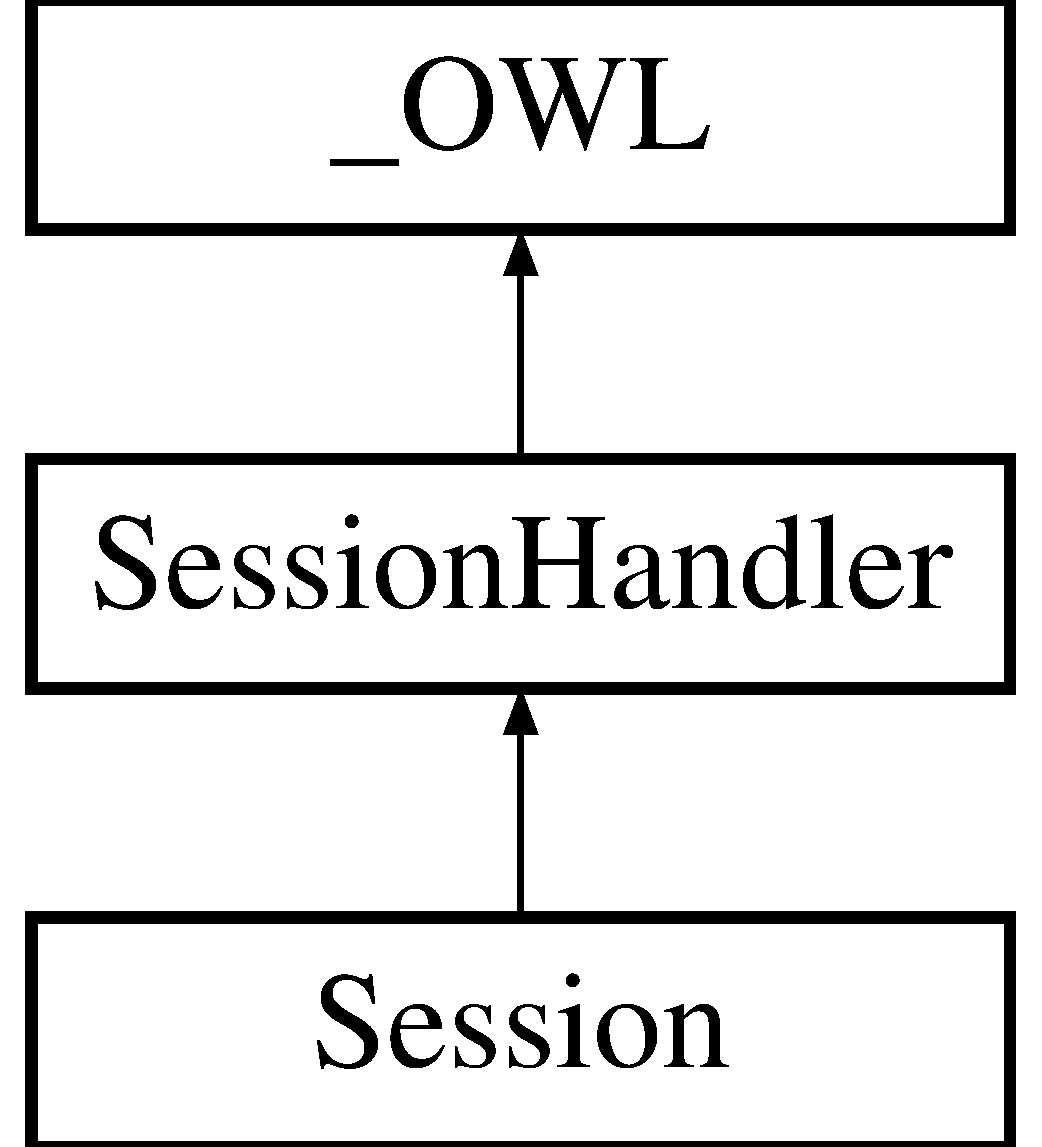
\includegraphics[height=3.000000cm]{classSession}
\end{center}
\end{figure}
\subsection*{Public Member Functions}
\begin{DoxyCompactItemize}
\item 
{\bf \_\-\_\-construct} ()
\item 
{\bf \_\-\_\-destruct} ()
\item 
{\bf newSession} ()
\item 
{\bf setRights} (\$bitmap, \$app={\bf OWL\_\-ID})
\item 
{\bf hasRight} (\$bit, \$appl)
\item 
{\bf setSessionVar} (\$var, \$val=0, \$flg={\bf SESSIONVAR\_\-SET})
\item 
{\bf getSessionVar} (\$var, \$default=null)
\item 
{\bf open} ()
\item 
{\bf close} ()
\item 
{\bf read} (\$id)
\item 
{\bf write} (\$id, \$data)
\item 
{\bf destroy} (\$id)
\item 
{\bf gc} (\$lifetime)
\item 
{\bf getStatus} ()
\item 
{\bf getSeverity} (\$status=null)
\item 
{\bf succeeded} (\$\_\-ok={\bf OWL\_\-SUCCESS}, \&\$\_\-object=null)
\item 
{\bf signal} (\$level={\bf OWL\_\-INFO}, \&\$text=false)
\item 
{\bf traceback} (\&\$text=false, \$depth=0)
\end{DoxyCompactItemize}
\subsection*{Protected Member Functions}
\begin{DoxyCompactItemize}
\item 
{\bf init} ()
\item 
{\bf setCallback} (\$\_\-dispatcher)
\item 
{\bf setCallbackArgument} (array \$\_\-arg)
\item 
{\bf getCallback} ()
\item 
{\bf reset} ()
\item 
{\bf saveStatus} ()
\item 
{\bf restoreStatus} ()
\item 
{\bf check} (\&\$object, \$level={\bf OWL\_\-WARNING})
\item 
{\bf setStatus} (\$status, \$params=array())
\item 
{\bf setHighSeverity} (\&\$object=null)
\end{DoxyCompactItemize}
\subsection*{Protected Attributes}
\begin{DoxyCompactItemize}
\item 
{\bf \$dataset} = null
\item 
{\bf \$severity}
\end{DoxyCompactItemize}
\subsection*{Private Member Functions}
\begin{DoxyCompactItemize}
\item 
{\bf restoreSession} ()
\item 
{\bf saveSession} ()
\item 
{\bf ipAddress} ()
\end{DoxyCompactItemize}
\subsection*{Private Attributes}
\begin{DoxyCompactItemize}
\item 
{\bf \$rights}
\end{DoxyCompactItemize}


\subsection{Detailed Description}
the OWL-\/PHP session object 

This class handles the \doxyref{OWL}{p.}{classOWL} session \begin{DoxyAuthor}{Author}
Oscar van Eijk, Oveas Functionality Provider 
\end{DoxyAuthor}
\begin{DoxyVersion}{Version}
Aug 13, 2008 -\/-\/ O van Eijk -\/-\/ initial version 
\end{DoxyVersion}


\subsection{Constructor \& Destructor Documentation}
\index{Session@{Session}!\_\-\_\-construct@{\_\-\_\-construct}}
\index{\_\-\_\-construct@{\_\-\_\-construct}!Session@{Session}}
\subsubsection[{\_\-\_\-construct}]{\setlength{\rightskip}{0pt plus 5cm}Session::\_\-\_\-construct (
\begin{DoxyParamCaption}
{}
\end{DoxyParamCaption}
)}\label{classSession_a36373ba15d6c8f932aeea02d7320d7c8}
When a new run is initialised, restore an older session or create a new one \begin{DoxyAuthor}{Author}
Oscar van Eijk, Oveas Functionality Provider 
\end{DoxyAuthor}


Reimplemented from {\bf SessionHandler} \doxyref{}{p.}{classSessionHandler_a546ba6d31a1ce532de13f65aadc3be0e}.



References ConfigHandler::get(), getSessionVar(), ipAddress(), newSession(), restoreSession(), setSessionVar(), and \_\-OWL::setStatus().

\index{Session@{Session}!\_\-\_\-destruct@{\_\-\_\-destruct}}
\index{\_\-\_\-destruct@{\_\-\_\-destruct}!Session@{Session}}
\subsubsection[{\_\-\_\-destruct}]{\setlength{\rightskip}{0pt plus 5cm}Session::\_\-\_\-destruct (
\begin{DoxyParamCaption}
{}
\end{DoxyParamCaption}
)}\label{classSession_aa498272c85524e4700abc3363883165b}
When a run ends, write the sessiondata \begin{DoxyAuthor}{Author}
Oscar van Eijk, Oveas Functionality Provider 
\end{DoxyAuthor}


Reimplemented from {\bf SessionHandler} \doxyref{}{p.}{classSessionHandler_a461097c3ee6b1aecf833ce1225d02329}.



References saveSession().



\subsection{Member Function Documentation}
\index{Session@{Session}!check@{check}}
\index{check@{check}!Session@{Session}}
\subsubsection[{check}]{\setlength{\rightskip}{0pt plus 5cm}\_\-OWL::check (
\begin{DoxyParamCaption}
\item[{\&\$}]{object, }
\item[{\$}]{level = {\ttfamily {\bf OWL\_\-WARNING}}}
\end{DoxyParamCaption}
)\hspace{0.3cm}{\ttfamily  [protected, inherited]}}\label{class__OWL_ae2e3c56e5f3c4ce4156c6b1bb1c50f63}
This is a helper function for lazy developers. Some checks have to be made quite often, this is a kinda macro to handle that. It compares the own severity level with that of a given object. If the highest level is above a given max, a traceback and reset are performed.


\begin{DoxyParams}[1]{Parameters}
\mbox{\tt in}  & {\em \$object} & Pointer to an object to check against \\
\hline
\mbox{\tt in}  & {\em \$level} & The maximum severity level \\
\hline
\end{DoxyParams}
\begin{DoxyReturn}{Returns}
True if the severity level was correct (below the max), otherwise false 
\end{DoxyReturn}
\begin{DoxyAuthor}{Author}
Oscar van Eijk, Oveas Functionality Provider 
\end{DoxyAuthor}


References \_\-OWL::reset(), \_\-OWL::setHighSeverity(), and \_\-OWL::traceback().



Referenced by SessionHandler::write().

\index{Session@{Session}!close@{close}}
\index{close@{close}!Session@{Session}}
\subsubsection[{close}]{\setlength{\rightskip}{0pt plus 5cm}SessionHandler::close (
\begin{DoxyParamCaption}
{}
\end{DoxyParamCaption}
)\hspace{0.3cm}{\ttfamily  [inherited]}}\label{classSessionHandler_a335ced83731c7e3e685b7e0df2989c79}
Close the session \begin{DoxyReturn}{Returns}
bool 
\end{DoxyReturn}
\begin{DoxyAuthor}{Author}
Oscar van Eijk, Oveas Functionality Provider 
\end{DoxyAuthor}
\index{Session@{Session}!destroy@{destroy}}
\index{destroy@{destroy}!Session@{Session}}
\subsubsection[{destroy}]{\setlength{\rightskip}{0pt plus 5cm}SessionHandler::destroy (
\begin{DoxyParamCaption}
\item[{\$}]{id}
\end{DoxyParamCaption}
)\hspace{0.3cm}{\ttfamily  [inherited]}}\label{classSessionHandler_a4e43712ef307979de1b12039ef801adb}
Destroy a session 
\begin{DoxyParams}[1]{Parameters}
\mbox{\tt in}  & {\em \$id} & ID of the session to destroy \\
\hline
\end{DoxyParams}
\begin{DoxyReturn}{Returns}
Boolean indicating success (true) or failure (false) 
\end{DoxyReturn}
\begin{DoxyAuthor}{Author}
Oscar van Eijk, Oveas Functionality Provider 
\end{DoxyAuthor}
\index{Session@{Session}!gc@{gc}}
\index{gc@{gc}!Session@{Session}}
\subsubsection[{gc}]{\setlength{\rightskip}{0pt plus 5cm}SessionHandler::gc (
\begin{DoxyParamCaption}
\item[{\$}]{lifetime}
\end{DoxyParamCaption}
)\hspace{0.3cm}{\ttfamily  [inherited]}}\label{classSessionHandler_ac33097332375ae3f8a43c31cef6db0e8}
Garbage Collector. By default, this has a 1\% change of being executed (session.gc\_\-probability/session.gc\_\-divisor). The values can be changed in the constructor. 
\begin{DoxyParams}[1]{Parameters}
\mbox{\tt in}  & {\em \$lifetime} & \doxyref{Session}{p.}{classSession} lifetime in seconds. By default, 1440 seconds. This can be changed in the constructor \\
\hline
\end{DoxyParams}
\begin{DoxyReturn}{Returns}
Status code 
\end{DoxyReturn}
\begin{DoxyAuthor}{Author}
Oscar van Eijk, Oveas Functionality Provider 
\end{DoxyAuthor}
\index{Session@{Session}!getCallback@{getCallback}}
\index{getCallback@{getCallback}!Session@{Session}}
\subsubsection[{getCallback}]{\setlength{\rightskip}{0pt plus 5cm}\_\-OWL::getCallback (
\begin{DoxyParamCaption}
{}
\end{DoxyParamCaption}
)\hspace{0.3cm}{\ttfamily  [protected, inherited]}}\label{class__OWL_acb46ff88f43ca66f1268d3f5199c3f8d}
Retrieve a previously set (callback) dispatcher. The (callback) dispatcher is cleared immediatly. \begin{DoxyReturn}{Returns}
The dispatcher, of null on failure. 
\end{DoxyReturn}
\begin{DoxyAuthor}{Author}
Oscar van Eijk, Oveas Functionality Provider 
\end{DoxyAuthor}


Reimplemented in {\bf Dispatcher} \doxyref{}{p.}{classDispatcher_a31c4bd4e4eaee7ef90b1ea364a901447}.



References OWL::factory().

\index{Session@{Session}!getSessionVar@{getSessionVar}}
\index{getSessionVar@{getSessionVar}!Session@{Session}}
\subsubsection[{getSessionVar}]{\setlength{\rightskip}{0pt plus 5cm}Session::getSessionVar (
\begin{DoxyParamCaption}
\item[{\$}]{var, }
\item[{\$}]{default = {\ttfamily null}}
\end{DoxyParamCaption}
)}\label{classSession_a473c338749db7d66f77663bfbe38fc87}
Get a session variable 
\begin{DoxyParams}[1]{Parameters}
\mbox{\tt in}  & {\em \$var} & Variable name \\
\hline
\mbox{\tt in}  & {\em \$default} & Default value to return if the variable was not set (default null) \\
\hline
\end{DoxyParams}
\begin{DoxyReturn}{Returns}
The value from the session, null if not set 
\end{DoxyReturn}
\begin{DoxyAuthor}{Author}
Oscar van Eijk, Oveas Functionality Provider 
\end{DoxyAuthor}


Referenced by \_\-\_\-construct(), and restoreSession().

\index{Session@{Session}!getSeverity@{getSeverity}}
\index{getSeverity@{getSeverity}!Session@{Session}}
\subsubsection[{getSeverity}]{\setlength{\rightskip}{0pt plus 5cm}\_\-OWL::getSeverity (
\begin{DoxyParamCaption}
\item[{\$}]{status = {\ttfamily null}}
\end{DoxyParamCaption}
)\hspace{0.3cm}{\ttfamily  [inherited]}}\label{class__OWL_a2374613f9bb7eccf49a5dbc9a9ef4751}
Get the current object severity level. 
\begin{DoxyParams}[1]{Parameters}
\mbox{\tt in}  & {\em \$status} & An optional parameter to check an other status code i.s.o the object's current status. \\
\hline
\end{DoxyParams}
\begin{DoxyReturn}{Returns}
Status severity level 
\end{DoxyReturn}
\begin{DoxyAuthor}{Author}
Oscar van Eijk, Oveas Functionality Provider 
\end{DoxyAuthor}


References \_\-OWL::\$status.



Referenced by LogHandler::composeMessage(), LogHandler::log(), and DataHandler::setKey().

\index{Session@{Session}!getStatus@{getStatus}}
\index{getStatus@{getStatus}!Session@{Session}}
\subsubsection[{getStatus}]{\setlength{\rightskip}{0pt plus 5cm}\_\-OWL::getStatus (
\begin{DoxyParamCaption}
{}
\end{DoxyParamCaption}
)\hspace{0.3cm}{\ttfamily  [final, inherited]}}\label{class__OWL_ac1f1643ff5b5db7c326c30477603358d}
Get the current object status. \begin{DoxyReturn}{Returns}
Object's status code 
\end{DoxyReturn}
\begin{DoxyAuthor}{Author}
Oscar van Eijk, Oveas Functionality Provider 
\end{DoxyAuthor}


Referenced by SchemeHandler::compare().

\index{Session@{Session}!hasRight@{hasRight}}
\index{hasRight@{hasRight}!Session@{Session}}
\subsubsection[{hasRight}]{\setlength{\rightskip}{0pt plus 5cm}Session::hasRight (
\begin{DoxyParamCaption}
\item[{\$}]{bit, }
\item[{\$}]{appl}
\end{DoxyParamCaption}
)}\label{classSession_a078e573c55453bb8c73a9f1321029d90}
Check if a rightsbit has been set for this session 
\begin{DoxyParams}[1]{Parameters}
\mbox{\tt in}  & {\em \$bit} & Rightsbit to check \\
\hline
\mbox{\tt in}  & {\em \$appl} & ID of the application the bit belongs to \\
\hline
\end{DoxyParams}
\begin{DoxyReturn}{Returns}
Boolean; true when the bit is set 
\end{DoxyReturn}
\begin{DoxyAuthor}{Author}
Oscar van Eijk, Oveas Functionality Provider 
\end{DoxyAuthor}
\index{Session@{Session}!init@{init}}
\index{init@{init}!Session@{Session}}
\subsubsection[{init}]{\setlength{\rightskip}{0pt plus 5cm}\_\-OWL::init (
\begin{DoxyParamCaption}
{}
\end{DoxyParamCaption}
)\hspace{0.3cm}{\ttfamily  [protected, inherited]}}\label{class__OWL_ae0ef3ded56e8a6b34b6461e5a721cd3e}
This function should be called by all constuctors. It initializes the general characteristics. Status is 'warning' by default, it's up to the contructor to set a proper status; if it's still 'warning', this $\ast$might$\ast$ indicate something went wrong. \begin{DoxyAuthor}{Author}
Oscar van Eijk, Oveas Functionality Provider 
\end{DoxyAuthor}


References OWL::factory(), and \_\-OWL::setStatus().



Referenced by FormFieldPlugin::\_\-\_\-construct(), Tablerow::\_\-\_\-construct(), Tablecell::\_\-\_\-construct(), Table::\_\-\_\-construct(), Document::\_\-\_\-construct(), ContainerPlugin::\_\-\_\-construct(), Container::\_\-\_\-construct(), SessionHandler::\_\-\_\-construct(), SchemeHandler::\_\-\_\-construct(), LogHandler::\_\-\_\-construct(), ImageHandler::\_\-\_\-construct(), FormHandler::\_\-\_\-construct(), FileHandler::\_\-\_\-construct(), DbHandler::\_\-\_\-construct(), DataHandler::\_\-\_\-construct(), OWL::\_\-\_\-construct(), Group::\_\-\_\-construct(), Form::\_\-\_\-construct(), Dispatcher::\_\-\_\-construct(), and User::construct().

\index{Session@{Session}!ipAddress@{ipAddress}}
\index{ipAddress@{ipAddress}!Session@{Session}}
\subsubsection[{ipAddress}]{\setlength{\rightskip}{0pt plus 5cm}Session::ipAddress (
\begin{DoxyParamCaption}
{}
\end{DoxyParamCaption}
)\hspace{0.3cm}{\ttfamily  [private]}}\label{classSession_a8e971d1175fb280898475673a2e7685a}
Identify the clients IP address where the client can use a shared internet source (HTTP\_\-CLIENT\_\-IP), a proxy server (HTTP\_\-X\_\-FORWARDED\_\-FOR) is direct access (REMOTE\_\-ADDR) \begin{DoxyReturn}{Returns}
The IP address, or 0.0.0.0 when none was found 
\end{DoxyReturn}
\begin{DoxyAuthor}{Author}
Oscar van Eijk, Oveas Functionality Provider 
\end{DoxyAuthor}


Referenced by \_\-\_\-construct(), and newSession().

\index{Session@{Session}!newSession@{newSession}}
\index{newSession@{newSession}!Session@{Session}}
\subsubsection[{newSession}]{\setlength{\rightskip}{0pt plus 5cm}Session::newSession (
\begin{DoxyParamCaption}
{}
\end{DoxyParamCaption}
)}\label{classSession_ad8a16f050a48c51bd060b7c6fb9e3ddf}
Initialize a session \begin{DoxyAuthor}{Author}
Oscar van Eijk, Oveas Functionality Provider 
\end{DoxyAuthor}


References ipAddress(), and setSessionVar().



Referenced by \_\-\_\-construct().

\index{Session@{Session}!open@{open}}
\index{open@{open}!Session@{Session}}
\subsubsection[{open}]{\setlength{\rightskip}{0pt plus 5cm}SessionHandler::open (
\begin{DoxyParamCaption}
{}
\end{DoxyParamCaption}
)\hspace{0.3cm}{\ttfamily  [inherited]}}\label{classSessionHandler_a50aa0b123f53d99de350a0eb02b4bfa5}
Open the session \begin{DoxyReturn}{Returns}
bool 
\end{DoxyReturn}
\begin{DoxyAuthor}{Author}
Oscar van Eijk, Oveas Functionality Provider 
\end{DoxyAuthor}
\index{Session@{Session}!read@{read}}
\index{read@{read}!Session@{Session}}
\subsubsection[{read}]{\setlength{\rightskip}{0pt plus 5cm}SessionHandler::read (
\begin{DoxyParamCaption}
\item[{\$}]{id}
\end{DoxyParamCaption}
)\hspace{0.3cm}{\ttfamily  [inherited]}}\label{classSessionHandler_a58cc3e5bf5b14e7bfbc73162de1f5d2b}
Read the session 
\begin{DoxyParams}[1]{Parameters}
\mbox{\tt in}  & {\em \$id} & session id \\
\hline
\end{DoxyParams}
\begin{DoxyReturn}{Returns}
\doxyref{Session}{p.}{classSession} data or null when not found 
\end{DoxyReturn}
\begin{DoxyAuthor}{Author}
Oscar van Eijk, Oveas Functionality Provider 
\end{DoxyAuthor}


References \_\-OWL::reset(), \_\-OWL::setHighSeverity(), and \_\-OWL::traceback().

\index{Session@{Session}!reset@{reset}}
\index{reset@{reset}!Session@{Session}}
\subsubsection[{reset}]{\setlength{\rightskip}{0pt plus 5cm}\_\-OWL::reset (
\begin{DoxyParamCaption}
{}
\end{DoxyParamCaption}
)\hspace{0.3cm}{\ttfamily  [protected, inherited]}}\label{class__OWL_a2f2a042bcf31965194c03033df0edc9b}
General reset function for all objects. Should be called after each non-\/fatal error \begin{DoxyAuthor}{Author}
Oscar van Eijk, Oveas Functionality Provider 
\end{DoxyAuthor}


Reimplemented in {\bf DbHandler} \doxyref{}{p.}{classDbHandler_a9982df4830f05803935bb31bac7fae3d}, and {\bf SchemeHandler} \doxyref{}{p.}{classSchemeHandler_aa25feb4a70d67b3d571904be4b2f50bc}.



References \_\-OWL::resetCalltree().



Referenced by \_\-OWL::check(), SessionHandler::read(), DataHandler::reset(), and \_\-OWL::setStatus().

\index{Session@{Session}!restoreSession@{restoreSession}}
\index{restoreSession@{restoreSession}!Session@{Session}}
\subsubsection[{restoreSession}]{\setlength{\rightskip}{0pt plus 5cm}Session::restoreSession (
\begin{DoxyParamCaption}
{}
\end{DoxyParamCaption}
)\hspace{0.3cm}{\ttfamily  [private]}}\label{classSession_aaf4c3729cd7374e4002c2e9c5ceb3de4}
Restore a session environment \begin{DoxyAuthor}{Author}
Oscar van Eijk, Oveas Functionality Provider 
\end{DoxyAuthor}


References getSessionVar().



Referenced by \_\-\_\-construct().

\index{Session@{Session}!restoreStatus@{restoreStatus}}
\index{restoreStatus@{restoreStatus}!Session@{Session}}
\subsubsection[{restoreStatus}]{\setlength{\rightskip}{0pt plus 5cm}\_\-OWL::restoreStatus (
\begin{DoxyParamCaption}
{}
\end{DoxyParamCaption}
)\hspace{0.3cm}{\ttfamily  [protected, inherited]}}\label{class__OWL_a93de01a9bbbc3f228e1a62a0740e90f0}
Restore the previously saved status object and destroy the copy \begin{DoxyAuthor}{Author}
Oscar van Eijk, Oveas Functionality Provider 
\end{DoxyAuthor}


References \_\-OWL::setStatus().



Referenced by User::logout().

\index{Session@{Session}!saveSession@{saveSession}}
\index{saveSession@{saveSession}!Session@{Session}}
\subsubsection[{saveSession}]{\setlength{\rightskip}{0pt plus 5cm}Session::saveSession (
\begin{DoxyParamCaption}
{}
\end{DoxyParamCaption}
)\hspace{0.3cm}{\ttfamily  [private]}}\label{classSession_a5bcd412ef78d844af9d69859a3df05b9}
Save active data to the session environment \begin{DoxyAuthor}{Author}
Oscar van Eijk, Oveas Functionality Provider 
\end{DoxyAuthor}


References setSessionVar().



Referenced by \_\-\_\-destruct().

\index{Session@{Session}!saveStatus@{saveStatus}}
\index{saveStatus@{saveStatus}!Session@{Session}}
\subsubsection[{saveStatus}]{\setlength{\rightskip}{0pt plus 5cm}\_\-OWL::saveStatus (
\begin{DoxyParamCaption}
{}
\end{DoxyParamCaption}
)\hspace{0.3cm}{\ttfamily  [protected, inherited]}}\label{class__OWL_add923dc756471318edca8883db3f4420}
Create a copy of the status object \begin{DoxyAuthor}{Author}
Oscar van Eijk, Oveas Functionality Provider 
\end{DoxyAuthor}


Referenced by User::logout().

\index{Session@{Session}!setCallback@{setCallback}}
\index{setCallback@{setCallback}!Session@{Session}}
\subsubsection[{setCallback}]{\setlength{\rightskip}{0pt plus 5cm}\_\-OWL::setCallback (
\begin{DoxyParamCaption}
\item[{\$}]{\_\-dispatcher}
\end{DoxyParamCaption}
)\hspace{0.3cm}{\ttfamily  [protected, inherited]}}\label{class__OWL_a5f84d43cd4dc7810649f1e2ebecad360}
Set a dispatcher for later callback 
\begin{DoxyParams}[1]{Parameters}
\mbox{\tt in}  & {\em \$\_\-dispatcher} & Dispatched, \\
\hline
\end{DoxyParams}
\begin{DoxySeeAlso}{See also}
\doxyref{Dispatcher::composeDispatcher()}{p.}{classDispatcher_a8a974bbbb30be7cda74f9929972fd2f6} 
\end{DoxySeeAlso}
\begin{DoxyReturn}{Returns}
True on success, false on failure 
\end{DoxyReturn}
\begin{DoxyAuthor}{Author}
Oscar van Eijk, Oveas Functionality Provider 
\end{DoxyAuthor}


References OWL::factory().

\index{Session@{Session}!setCallbackArgument@{setCallbackArgument}}
\index{setCallbackArgument@{setCallbackArgument}!Session@{Session}}
\subsubsection[{setCallbackArgument}]{\setlength{\rightskip}{0pt plus 5cm}\_\-OWL::setCallbackArgument (
\begin{DoxyParamCaption}
\item[{array \$}]{\_\-arg}
\end{DoxyParamCaption}
)\hspace{0.3cm}{\ttfamily  [protected, inherited]}}\label{class__OWL_a4e9ebfbd3c0d76539bed4e44de9962c3}
Add an argument to a previously registered callback dispatcher 
\begin{DoxyParams}[1]{Parameters}
\mbox{\tt in}  & {\em \$\_\-arg} & Argument, must be an array type. When non-\/ arrays should be passed as arguments, the must be set when the callback is registered already \\
\hline
\end{DoxyParams}
\begin{DoxyReturn}{Returns}
True on success, false on failure 
\end{DoxyReturn}
\begin{DoxyAuthor}{Author}
Oscar van Eijk, Oveas Functionality Provider 
\end{DoxyAuthor}


References OWL::factory().



Referenced by User::register().

\index{Session@{Session}!setHighSeverity@{setHighSeverity}}
\index{setHighSeverity@{setHighSeverity}!Session@{Session}}
\subsubsection[{setHighSeverity}]{\setlength{\rightskip}{0pt plus 5cm}\_\-OWL::setHighSeverity (
\begin{DoxyParamCaption}
\item[{\&\$}]{object = {\ttfamily null}}
\end{DoxyParamCaption}
)\hspace{0.3cm}{\ttfamily  [protected, inherited]}}\label{class__OWL_a97173dbe452428d3851406413264734d}
Compare the severity level of the current object with a given one and set my statuspointer to the object with the highest level. \begin{DoxyAuthor}{Author}
Oscar van Eijk, Oveas Functionality Provider 
\end{DoxyAuthor}


Referenced by \_\-OWL::check(), DataHandler::db(), DataHandler::prepare(), and SessionHandler::read().

\index{Session@{Session}!setRights@{setRights}}
\index{setRights@{setRights}!Session@{Session}}
\subsubsection[{setRights}]{\setlength{\rightskip}{0pt plus 5cm}Session::setRights (
\begin{DoxyParamCaption}
\item[{\$}]{bitmap, }
\item[{\$}]{app = {\ttfamily {\bf OWL\_\-ID}}}
\end{DoxyParamCaption}
)}\label{classSession_a89b56dcf33065fe9c745979d3ab3d90e}
Set the default right bitmap for this session 
\begin{DoxyParams}[1]{Parameters}
\mbox{\tt in}  & {\em \$bitmap} & The bitmap value which is either the default group value, or the complete list of rights for this user (depending on the configuration) \\
\hline
\mbox{\tt in}  & {\em \$app} & Application ID \\
\hline
\end{DoxyParams}
\begin{DoxyAuthor}{Author}
Oscar van Eijk, Oveas Functionality Provider 
\end{DoxyAuthor}
\index{Session@{Session}!setSessionVar@{setSessionVar}}
\index{setSessionVar@{setSessionVar}!Session@{Session}}
\subsubsection[{setSessionVar}]{\setlength{\rightskip}{0pt plus 5cm}Session::setSessionVar (
\begin{DoxyParamCaption}
\item[{\$}]{var, }
\item[{\$}]{val = {\ttfamily 0}, }
\item[{\$}]{flg = {\ttfamily {\bf SESSIONVAR\_\-SET}}}
\end{DoxyParamCaption}
)}\label{classSession_a664b79807cf89f0259e051fcc2a6c274}
Set a session variable 
\begin{DoxyParams}[1]{Parameters}
\mbox{\tt in}  & {\em \$var} & Variable name \\
\hline
\mbox{\tt in}  & {\em \$val} & Variable value (default 0) \\
\hline
\mbox{\tt in}  & {\em \$flg} & How to handle the value. Default SESSIONVAR\_\-SET \\
\hline
\end{DoxyParams}
\begin{DoxyAuthor}{Author}
Oscar van Eijk, Oveas Functionality Provider 
\end{DoxyAuthor}


Referenced by \_\-\_\-construct(), newSession(), and saveSession().

\index{Session@{Session}!setStatus@{setStatus}}
\index{setStatus@{setStatus}!Session@{Session}}
\subsubsection[{setStatus}]{\setlength{\rightskip}{0pt plus 5cm}\_\-OWL::setStatus (
\begin{DoxyParamCaption}
\item[{\$}]{status, }
\item[{\$}]{params = {\ttfamily array~()}}
\end{DoxyParamCaption}
)\hspace{0.3cm}{\ttfamily  [final, protected, inherited]}}\label{class__OWL_a80e2fe01c3663dbb0ab685eebe33fd1e}
Set the current object status to the specified value. 
\begin{DoxyParams}[1]{Parameters}
\mbox{\tt in}  & {\em \$status} & \doxyref{OWL}{p.}{classOWL} status code \\
\hline
\mbox{\tt in}  & {\em \$params} & \\
\hline
\end{DoxyParams}
\begin{DoxyAuthor}{Author}
Oscar van Eijk, Oveas Functionality Provider 
\end{DoxyAuthor}


References \$GLOBALS, \_\-OWL::\$status, ConfigHandler::get(), Register::getCode(), \_\-OWL::reset(), and \_\-OWL::signal().



Referenced by DbHandler::\_\-\_\-clone(), Container::\_\-\_\-construct(), SchemeHandler::\_\-\_\-construct(), ImageHandler::\_\-\_\-construct(), FormHandler::\_\-\_\-construct(), FileHandler::\_\-\_\-construct(), DbHandler::\_\-\_\-construct(), DataHandler::\_\-\_\-construct(), \_\-\_\-construct(), BaseElement::\_\-getContent(), Form::addField(), FormFieldRadioPlugin::addOption(), BaseElement::addToContent(), DbHandler::alt(), SchemeHandler::alterScheme(), FileHandler::close(), DbHandler::commitTransaction(), Dispatcher::composeDispatcher(), User::confirm(), DbHandler::connect(), DbHandler::create(), SchemeHandler::createScheme(), SchemeHandler::defineIndex(), SchemeHandler::defineScheme(), Dispatcher::dispatch(), FormHandler::get(), DataHandler::get(), SchemeHandler::getTableColumns(), SchemeHandler::getTableIndexes(), \_\-OWL::init(), Document::loadScript(), Document::loadStyle(), User::login(), FileHandler::open(), DbHandler::open(), LogHandler::openLogfile(), DataHandler::prepare(), DbHandler::prepareDelete(), DbHandler::prepareField(), DbHandler::prepareInsert(), DbHandler::prepareRead(), DbHandler::prepareUpdate(), DbHandler::read(), FileHandler::readLine(), User::readUserdata(), User::register(), Dispatcher::registerArgument(), Dispatcher::registerCallback(), \_\-OWL::restoreStatus(), DbHandler::rollbackTransaction(), SchemeHandler::scheme(), FormHandler::set(), BaseElement::setAttributes(), BaseElement::setContent(), Form::setEncoding(), Document::setFavicon(), Form::setFieldAttributes(), DataHandler::setJoin(), DataHandler::setKey(), FormFieldTextPlugin::setMaxsize(), Document::setMeta(), Form::setMethod(), FormFieldRadioPlugin::setSelected(), FormFieldTextPlugin::setSize(), FormFieldSelectPlugin::setSize(), FormFieldSelectPlugin::setValue(), Form::showField(), DbHandler::startTransaction(), SchemeHandler::tableDescription(), SchemeHandler::validateScheme(), and DbHandler::write().

\index{Session@{Session}!signal@{signal}}
\index{signal@{signal}!Session@{Session}}
\subsubsection[{signal}]{\setlength{\rightskip}{0pt plus 5cm}\_\-OWL::signal (
\begin{DoxyParamCaption}
\item[{\$}]{level = {\ttfamily {\bf OWL\_\-INFO}}, }
\item[{\&\$}]{text = {\ttfamily false}}
\end{DoxyParamCaption}
)\hspace{0.3cm}{\ttfamily  [inherited]}}\label{class__OWL_a51ba4a16409acf2a2f61f286939091a5}
Display the message for the current object status 
\begin{DoxyParams}[1]{Parameters}
\mbox{\tt in}  & {\em \$level} & An optional severity level; message will only be displayed when it is at least of this level. \\
\hline
\mbox{\tt out}  & {\em \$text} & If this parameter is given, the message text is returned in this string instead of echood. \\
\hline
\end{DoxyParams}
\begin{DoxyReturn}{Returns}
The severity level for this object 
\end{DoxyReturn}
\begin{DoxyAuthor}{Author}
Oscar van Eijk, Oveas Functionality Provider 
\end{DoxyAuthor}


References ConfigHandler::get().



Referenced by \_\-OWL::setStatus(), and \_\-OWL::traceback().

\index{Session@{Session}!succeeded@{succeeded}}
\index{succeeded@{succeeded}!Session@{Session}}
\subsubsection[{succeeded}]{\setlength{\rightskip}{0pt plus 5cm}\_\-OWL::succeeded (
\begin{DoxyParamCaption}
\item[{\$}]{\_\-ok = {\ttfamily {\bf OWL\_\-SUCCESS}}, }
\item[{\&\$}]{\_\-object = {\ttfamily null}}
\end{DoxyParamCaption}
)\hspace{0.3cm}{\ttfamily  [inherited]}}\label{class__OWL_a53ab4d3bbb2c6a56966c339ca4b4c805}
Check if the object currenlty has a success state 
\begin{DoxyParams}[1]{Parameters}
\mbox{\tt in}  & {\em \$\_\-ok} & The highest severity that's considered successfull, default OWL\_\-SUCCESS \\
\hline
\mbox{\tt in}  & {\em \$\_\-object} & REference to the object to check, defaults to the current object \\
\hline
\end{DoxyParams}
\begin{DoxyReturn}{Returns}
Boolean true when successfull 
\end{DoxyReturn}
\begin{DoxyAuthor}{Author}
Oscar van Eijk, Oveas Functionality Provider 
\end{DoxyAuthor}


Referenced by User::construct(), Dispatcher::registerArgument(), and Dispatcher::registerCallback().

\index{Session@{Session}!traceback@{traceback}}
\index{traceback@{traceback}!Session@{Session}}
\subsubsection[{traceback}]{\setlength{\rightskip}{0pt plus 5cm}\_\-OWL::traceback (
\begin{DoxyParamCaption}
\item[{\&\$}]{text = {\ttfamily false}, }
\item[{\$}]{depth = {\ttfamily 0}}
\end{DoxyParamCaption}
)\hspace{0.3cm}{\ttfamily  [inherited]}}\label{class__OWL_aa29547995d6741b7d2b90c1d4ea99a13}
If somehwere in the nested calls an error occured, we can traceback the original failing object with this function and signal the message. 
\begin{DoxyParams}[1]{Parameters}
\mbox{\tt out}  & {\em \$text} & Optional variable in which the message text can be stored. If not given, the text will be written to standard output \\
\hline
\mbox{\tt in}  & {\em \$depth} & This paramater should be initially empty. It calculates the depth in recursive calls. \\
\hline
\end{DoxyParams}
\begin{DoxyReturn}{Returns}
Severity code of the failing object 
\end{DoxyReturn}
\begin{DoxyAuthor}{Author}
Oscar van Eijk, Oveas Functionality Provider 
\end{DoxyAuthor}


References \_\-OWL::signal().



Referenced by \_\-OWL::check(), User::login(), and SessionHandler::read().

\index{Session@{Session}!write@{write}}
\index{write@{write}!Session@{Session}}
\subsubsection[{write}]{\setlength{\rightskip}{0pt plus 5cm}SessionHandler::write (
\begin{DoxyParamCaption}
\item[{\$}]{id, }
\item[{\$}]{data}
\end{DoxyParamCaption}
)\hspace{0.3cm}{\ttfamily  [inherited]}}\label{classSessionHandler_ab59071ef0d3deee2472c6916471bd9f5}
Write the session 
\begin{DoxyParams}[1]{Parameters}
\mbox{\tt in}  & {\em \$id} & \doxyref{Session}{p.}{classSession} id \\
\hline
\mbox{\tt in}  & {\em \$data} & \doxyref{Session}{p.}{classSession} data \\
\hline
\end{DoxyParams}
\begin{DoxyReturn}{Returns}
True on success, Failure otherwise 
\end{DoxyReturn}
\begin{DoxyAuthor}{Author}
Oscar van Eijk, Oveas Functionality Provider 
\end{DoxyAuthor}


References \_\-OWL::check().



\subsection{Member Data Documentation}
\index{Session@{Session}!\$dataset@{\$dataset}}
\index{\$dataset@{\$dataset}!Session@{Session}}
\subsubsection[{\$dataset}]{\setlength{\rightskip}{0pt plus 5cm}SessionHandler::\$dataset = null\hspace{0.3cm}{\ttfamily  [protected, inherited]}}\label{classSessionHandler_a74c46fcfbadd4c4e6bacc73ddf350056}
Link to a datahandler object. This dataset is used as an interface to all database IO. \index{Session@{Session}!\$rights@{\$rights}}
\index{\$rights@{\$rights}!Session@{Session}}
\subsubsection[{\$rights}]{\setlength{\rightskip}{0pt plus 5cm}Session::\$rights\hspace{0.3cm}{\ttfamily  [private]}}\label{classSession_a83d6397ee36c98e8799a663e2b67c025}
Right object holding the currently active right for this session \index{Session@{Session}!\$severity@{\$severity}}
\index{\$severity@{\$severity}!Session@{Session}}
\subsubsection[{\$severity}]{\setlength{\rightskip}{0pt plus 5cm}\_\-OWL::\$severity\hspace{0.3cm}{\ttfamily  [protected, inherited]}}\label{class__OWL_ad26b40a9dbbacb33e299b17826f8327c}
Severity level of the current object status 

Referenced by DbHandler::commitTransaction(), DbHandler::rollbackTransaction(), and DbHandler::startTransaction().



The documentation for this class was generated from the following file:\begin{DoxyCompactItemize}
\item 
/home/oscar/projects/owl-\/php/src/kernel/bo/{\bf class.session.php}\end{DoxyCompactItemize}

\section{SessionHandler Class Reference}
\label{classSessionHandler}\index{SessionHandler@{SessionHandler}}


the PHP session object  




Inheritance diagram for SessionHandler:\nopagebreak
\begin{figure}[H]
\begin{center}
\leavevmode
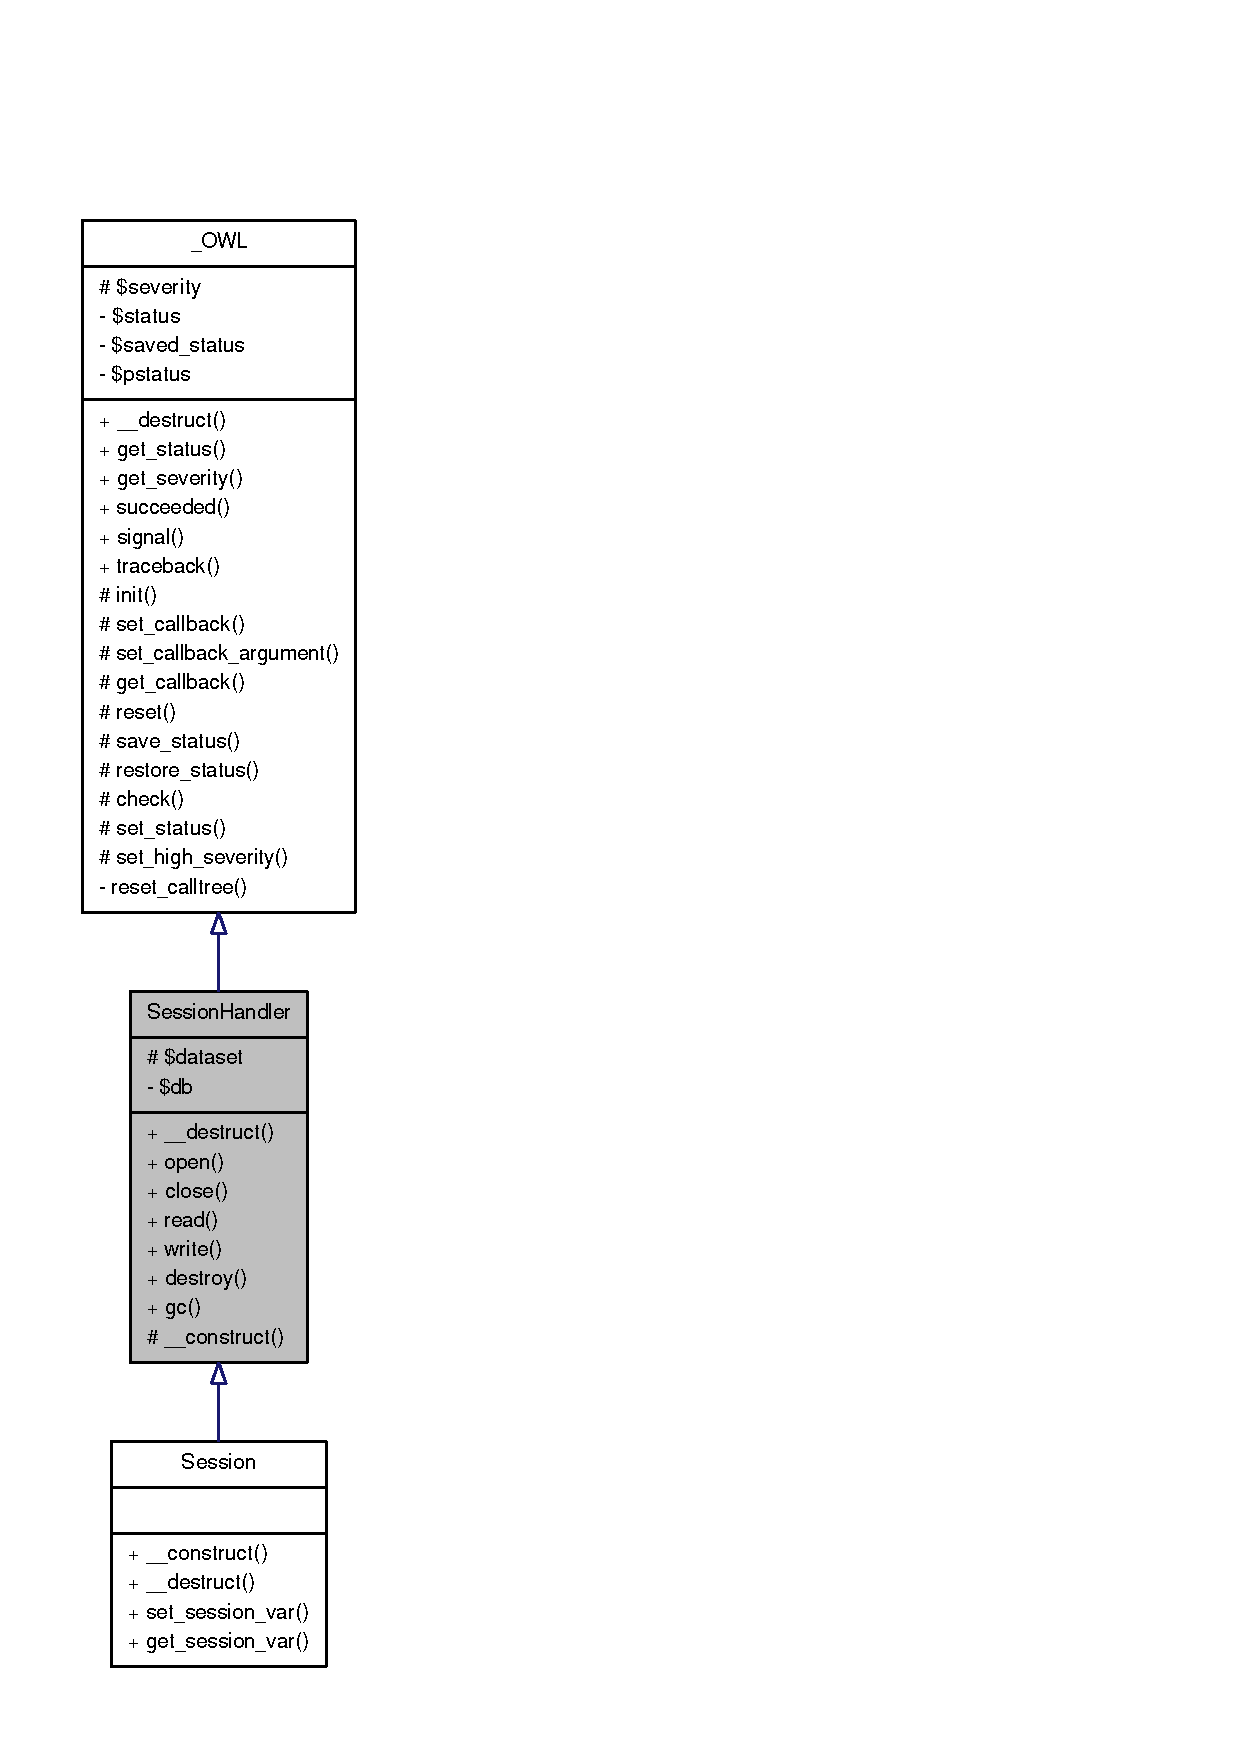
\includegraphics[height=400pt]{classSessionHandler__inherit__graph}
\end{center}
\end{figure}


Collaboration diagram for SessionHandler:\nopagebreak
\begin{figure}[H]
\begin{center}
\leavevmode
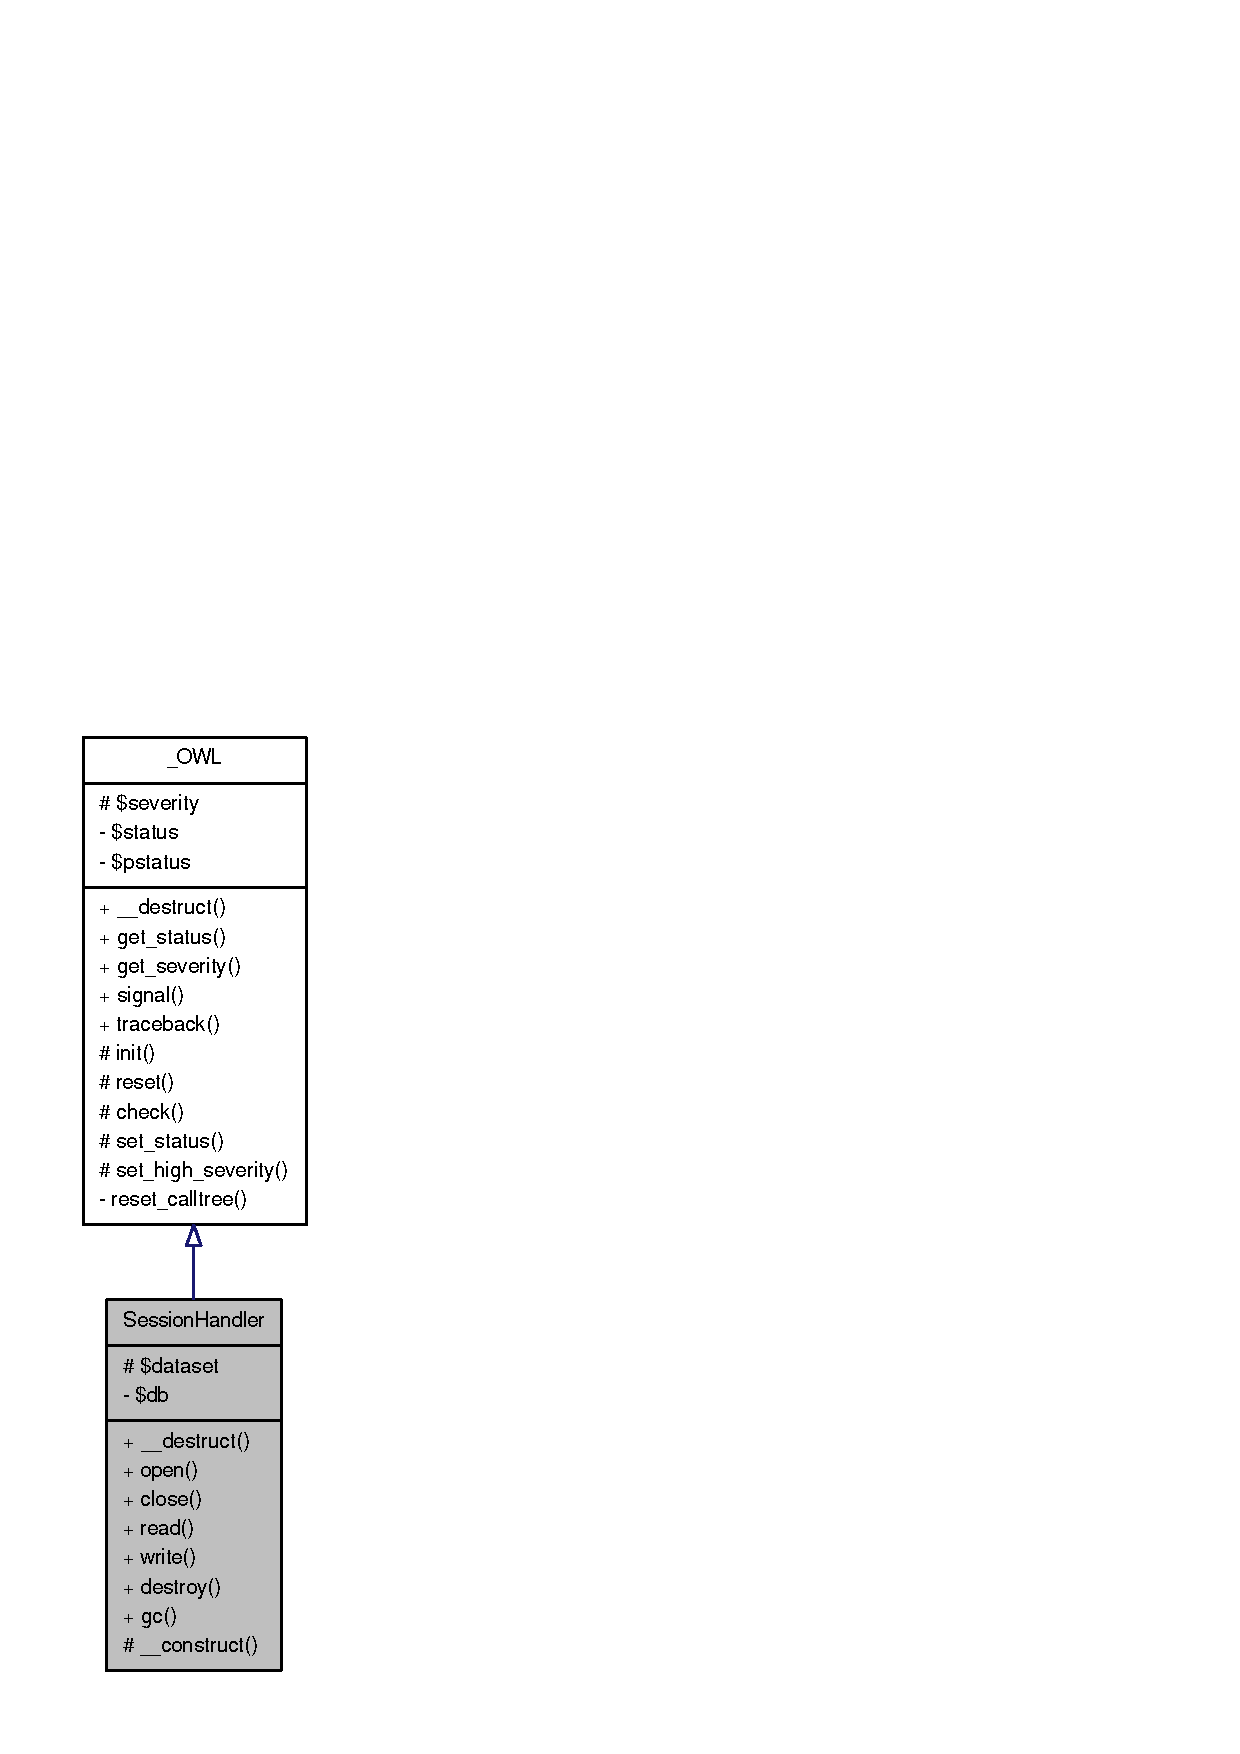
\includegraphics[height=400pt]{classSessionHandler__coll__graph}
\end{center}
\end{figure}
\subsection*{Public Member Functions}
\begin{DoxyCompactItemize}
\item 
\hyperlink{classSessionHandler_a461097c3ee6b1aecf833ce1225d02329}{\_\-\_\-destruct} ()
\item 
\hyperlink{classSessionHandler_a50aa0b123f53d99de350a0eb02b4bfa5}{open} ()
\item 
\hyperlink{classSessionHandler_a335ced83731c7e3e685b7e0df2989c79}{close} ()
\item 
\hyperlink{classSessionHandler_a58cc3e5bf5b14e7bfbc73162de1f5d2b}{read} (\$id)
\item 
\hyperlink{classSessionHandler_ab59071ef0d3deee2472c6916471bd9f5}{write} (\$id, \$data)
\item 
\hyperlink{classSessionHandler_a4e43712ef307979de1b12039ef801adb}{destroy} (\$id)
\item 
\hyperlink{classSessionHandler_ac33097332375ae3f8a43c31cef6db0e8}{gc} (\$lifetime)
\item 
\hyperlink{class__OWL_a99ec771fa2c5c279f80152cc09e489a8}{get\_\-status} ()
\item 
\hyperlink{class__OWL_adf9509ef96858be7bdd9414c5ef129aa}{get\_\-severity} (\$status=null)
\item 
\hyperlink{class__OWL_a51ba4a16409acf2a2f61f286939091a5}{signal} (\$level=\hyperlink{owl_8severitycodes_8php_a139328861128689f2f4def6a399d9057}{OWL\_\-INFO}, \&\$text=false)
\item 
\hyperlink{class__OWL_aa29547995d6741b7d2b90c1d4ea99a13}{traceback} (\&\$text=false, \$depth=0)
\end{DoxyCompactItemize}
\subsection*{Protected Member Functions}
\begin{DoxyCompactItemize}
\item 
\hyperlink{classSessionHandler_a546ba6d31a1ce532de13f65aadc3be0e}{\_\-\_\-construct} ()
\item 
\hyperlink{class__OWL_ae0ef3ded56e8a6b34b6461e5a721cd3e}{init} ()
\item 
\hyperlink{class__OWL_a2f2a042bcf31965194c03033df0edc9b}{reset} ()
\item 
\hyperlink{class__OWL_ad6f4f6946f40199dd0333cf219fa500e}{check} (\&\$object, \$level)
\item 
\hyperlink{class__OWL_aea912d0ede9b3c2a69b79072d94d4787}{set\_\-status} (\$status, \$params=array())
\item 
\hyperlink{class__OWL_a576829692a3b66e3d518853bf43abae3}{set\_\-high\_\-severity} (\&\$object=null)
\end{DoxyCompactItemize}
\subsection*{Protected Attributes}
\begin{DoxyCompactItemize}
\item 
\hyperlink{classSessionHandler_a74c46fcfbadd4c4e6bacc73ddf350056}{\$dataset}
\item 
\hyperlink{class__OWL_ad26b40a9dbbacb33e299b17826f8327c}{\$severity}
\end{DoxyCompactItemize}
\subsection*{Private Attributes}
\begin{DoxyCompactItemize}
\item 
\hyperlink{classSessionHandler_a0bb7c3206f3664f2a4b8e96edf49a3bc}{\$db}
\end{DoxyCompactItemize}


\subsection{Detailed Description}
the PHP session object This class saves and (re)stores the user sessions \begin{DoxyAuthor}{Author}
Oscar van Eijk, Oveas Functionality Provider 
\end{DoxyAuthor}
\begin{DoxyVersion}{Version}
Jul 29, 2008 -\/-\/ O van Eijk -\/-\/ initial version 
\end{DoxyVersion}


\subsection{Constructor \& Destructor Documentation}
\index{SessionHandler@{SessionHandler}!\_\-\_\-construct@{\_\-\_\-construct}}
\index{\_\-\_\-construct@{\_\-\_\-construct}!SessionHandler@{SessionHandler}}
\subsubsection[{\_\-\_\-construct}]{\setlength{\rightskip}{0pt plus 5cm}SessionHandler::\_\-\_\-construct ()\hspace{0.3cm}{\ttfamily  \mbox{[}protected\mbox{]}}}\label{classSessionHandler_a546ba6d31a1ce532de13f65aadc3be0e}
Class constructor; set the save\_\-handler 

Reimplemented in \hyperlink{classSession_a36373ba15d6c8f932aeea02d7320d7c8}{Session}.



References DbHandler::get\_\-instance(), \_\-OWL::init(), and \_\-OWL::set\_\-status().

\index{SessionHandler@{SessionHandler}!\_\-\_\-destruct@{\_\-\_\-destruct}}
\index{\_\-\_\-destruct@{\_\-\_\-destruct}!SessionHandler@{SessionHandler}}
\subsubsection[{\_\-\_\-destruct}]{\setlength{\rightskip}{0pt plus 5cm}SessionHandler::\_\-\_\-destruct ()}\label{classSessionHandler_a461097c3ee6b1aecf833ce1225d02329}
Write the session data back to the database 

Reimplemented from \hyperlink{class__OWL_a44fd2222476a3109286cc82d92b6bbcc}{\_\-OWL}.



Reimplemented in \hyperlink{classSession_aa498272c85524e4700abc3363883165b}{Session}.



\subsection{Member Function Documentation}
\index{SessionHandler@{SessionHandler}!check@{check}}
\index{check@{check}!SessionHandler@{SessionHandler}}
\subsubsection[{check}]{\setlength{\rightskip}{0pt plus 5cm}\_\-OWL::check (\&\$ {\em object}, \/  \$ {\em level})\hspace{0.3cm}{\ttfamily  \mbox{[}protected, inherited\mbox{]}}}\label{class__OWL_ad6f4f6946f40199dd0333cf219fa500e}
This is a helper function for lazy developers. Some checks have to be made quite often, this is a kinda macro to handle that. It compares the own severity level with that of a given object. If the highest level is above a given max, a traceback and reset are performed.


\begin{DoxyParams}{Parameters}
\item[\mbox{$\leftarrow$} {\em \$object}]Pointer to an object to check against \item[\mbox{$\leftarrow$} {\em \$level}]The maximum severity level \end{DoxyParams}
\begin{DoxyReturn}{Returns}
True if the severity level was correct ( below the max), otherwise false 
\end{DoxyReturn}


References \_\-OWL::reset(), \_\-OWL::set\_\-high\_\-severity(), and \_\-OWL::traceback().



Referenced by write().

\index{SessionHandler@{SessionHandler}!close@{close}}
\index{close@{close}!SessionHandler@{SessionHandler}}
\subsubsection[{close}]{\setlength{\rightskip}{0pt plus 5cm}SessionHandler::close ()}\label{classSessionHandler_a335ced83731c7e3e685b7e0df2989c79}
Close the session

\begin{DoxyReturn}{Returns}
bool 
\end{DoxyReturn}
\index{SessionHandler@{SessionHandler}!destroy@{destroy}}
\index{destroy@{destroy}!SessionHandler@{SessionHandler}}
\subsubsection[{destroy}]{\setlength{\rightskip}{0pt plus 5cm}SessionHandler::destroy (\$ {\em id})}\label{classSessionHandler_a4e43712ef307979de1b12039ef801adb}
Destroy a session


\begin{DoxyParams}{Parameters}
\item[\mbox{$\leftarrow$} {\em \$id}]ID of the session to destroy \end{DoxyParams}
\begin{DoxyReturn}{Returns}
Boolean indicating success (true) or failure (false) 
\end{DoxyReturn}
\index{SessionHandler@{SessionHandler}!gc@{gc}}
\index{gc@{gc}!SessionHandler@{SessionHandler}}
\subsubsection[{gc}]{\setlength{\rightskip}{0pt plus 5cm}SessionHandler::gc (\$ {\em lifetime})}\label{classSessionHandler_ac33097332375ae3f8a43c31cef6db0e8}
Garbage Collector. By default, this has a 1\% change of being executed (session.gc\_\-probability/session.gc\_\-divisor). The values can be changed in the constructor.


\begin{DoxyParams}{Parameters}
\item[\mbox{$\leftarrow$} {\em \$lifetime}]\hyperlink{classSession}{Session} lifetime in seconds. By default, 1440 seconds. This can be changed in the constructor \end{DoxyParams}
\begin{DoxyReturn}{Returns}
Status code 
\end{DoxyReturn}
\index{SessionHandler@{SessionHandler}!get\_\-severity@{get\_\-severity}}
\index{get\_\-severity@{get\_\-severity}!SessionHandler@{SessionHandler}}
\subsubsection[{get\_\-severity}]{\setlength{\rightskip}{0pt plus 5cm}\_\-OWL::get\_\-severity (\$ {\em status} = {\ttfamily null})\hspace{0.3cm}{\ttfamily  \mbox{[}inherited\mbox{]}}}\label{class__OWL_adf9509ef96858be7bdd9414c5ef129aa}
Get the current object severity level.


\begin{DoxyParams}{Parameters}
\item[\mbox{$\leftarrow$} {\em \$status}]An optional parameter to check an other status code i.s.o the object's current status. \end{DoxyParams}
\begin{DoxyReturn}{Returns}
Status severity level 
\end{DoxyReturn}


References \_\-OWL::\$status.



Referenced by LogHandler::compose\_\-message(), LogHandler::log(), and DataHandler::set\_\-key().

\index{SessionHandler@{SessionHandler}!get\_\-status@{get\_\-status}}
\index{get\_\-status@{get\_\-status}!SessionHandler@{SessionHandler}}
\subsubsection[{get\_\-status}]{\setlength{\rightskip}{0pt plus 5cm}\_\-OWL::get\_\-status ()\hspace{0.3cm}{\ttfamily  \mbox{[}final, inherited\mbox{]}}}\label{class__OWL_a99ec771fa2c5c279f80152cc09e489a8}
Get the current object status.

\begin{DoxyReturn}{Returns}
Object's status code 
\end{DoxyReturn}


Referenced by FormHandler::\_\-\_\-get().

\index{SessionHandler@{SessionHandler}!init@{init}}
\index{init@{init}!SessionHandler@{SessionHandler}}
\subsubsection[{init}]{\setlength{\rightskip}{0pt plus 5cm}\_\-OWL::init ()\hspace{0.3cm}{\ttfamily  \mbox{[}protected, inherited\mbox{]}}}\label{class__OWL_ae0ef3ded56e8a6b34b6461e5a721cd3e}
This function should be called by all constuctors. It initializes the general characteristics. Status is 'warning' by default, it's up to the contructor to set a proper status; if it's still 'warning', this $\ast$might$\ast$ indicate something went wrong. 

References OWL::factory().



Referenced by DOMElement::\_\-\_\-construct(), UserHandler::\_\-\_\-construct(), \_\-\_\-construct(), LogHandler::\_\-\_\-construct(), FileHandler::\_\-\_\-construct(), DbHandler::\_\-\_\-construct(), OWL::\_\-\_\-construct(), and DataHandler::DataHandler().

\index{SessionHandler@{SessionHandler}!open@{open}}
\index{open@{open}!SessionHandler@{SessionHandler}}
\subsubsection[{open}]{\setlength{\rightskip}{0pt plus 5cm}SessionHandler::open ()}\label{classSessionHandler_a50aa0b123f53d99de350a0eb02b4bfa5}
Open the session

\begin{DoxyReturn}{Returns}
bool 
\end{DoxyReturn}
\index{SessionHandler@{SessionHandler}!read@{read}}
\index{read@{read}!SessionHandler@{SessionHandler}}
\subsubsection[{read}]{\setlength{\rightskip}{0pt plus 5cm}SessionHandler::read (\$ {\em id})}\label{classSessionHandler_a58cc3e5bf5b14e7bfbc73162de1f5d2b}
Read the session


\begin{DoxyParams}{Parameters}
\item[\mbox{$\leftarrow$} {\em \$id}]session id \end{DoxyParams}
\begin{DoxyReturn}{Returns}
\hyperlink{classSession}{Session} data 
\end{DoxyReturn}


References \_\-OWL::reset(), \_\-OWL::set\_\-high\_\-severity(), and \_\-OWL::traceback().

\index{SessionHandler@{SessionHandler}!reset@{reset}}
\index{reset@{reset}!SessionHandler@{SessionHandler}}
\subsubsection[{reset}]{\setlength{\rightskip}{0pt plus 5cm}\_\-OWL::reset ()\hspace{0.3cm}{\ttfamily  \mbox{[}protected, inherited\mbox{]}}}\label{class__OWL_a2f2a042bcf31965194c03033df0edc9b}
General reset function for all objects. Should be called after each non-\/fatal error 

Reimplemented in \hyperlink{classDbHandler_a9982df4830f05803935bb31bac7fae3d}{DbHandler}.



References \_\-OWL::reset\_\-calltree().



Referenced by \_\-OWL::check(), read(), DataHandler::reset(), and \_\-OWL::set\_\-status().

\index{SessionHandler@{SessionHandler}!set\_\-high\_\-severity@{set\_\-high\_\-severity}}
\index{set\_\-high\_\-severity@{set\_\-high\_\-severity}!SessionHandler@{SessionHandler}}
\subsubsection[{set\_\-high\_\-severity}]{\setlength{\rightskip}{0pt plus 5cm}\_\-OWL::set\_\-high\_\-severity (\&\$ {\em object} = {\ttfamily null})\hspace{0.3cm}{\ttfamily  \mbox{[}protected, inherited\mbox{]}}}\label{class__OWL_a576829692a3b66e3d518853bf43abae3}
Compare the severity level of the current object with a given one and set my statuspointer to the object with the highest level. 

Referenced by \_\-OWL::check(), DataHandler::db(), DataHandler::prepare(), and read().

\index{SessionHandler@{SessionHandler}!set\_\-status@{set\_\-status}}
\index{set\_\-status@{set\_\-status}!SessionHandler@{SessionHandler}}
\subsubsection[{set\_\-status}]{\setlength{\rightskip}{0pt plus 5cm}\_\-OWL::set\_\-status (\$ {\em status}, \/  \$ {\em params} = {\ttfamily array~()})\hspace{0.3cm}{\ttfamily  \mbox{[}final, protected, inherited\mbox{]}}}\label{class__OWL_aea912d0ede9b3c2a69b79072d94d4787}
Set the current object status to the specified value.


\begin{DoxyParams}{Parameters}
\item[\mbox{$\leftarrow$} {\em \$status}]\hyperlink{classOWL}{OWL} status code \item[\mbox{$\leftarrow$} {\em \$params}]\end{DoxyParams}


References \$GLOBALS, \_\-OWL::\$status, ConfigHandler::get(), Register::get\_\-code(), \_\-OWL::reset(), and \_\-OWL::signal().



Referenced by UserHandler::\_\-\_\-construct(), \_\-\_\-construct(), FormHandler::\_\-\_\-construct(), FileHandler::\_\-\_\-construct(), DbHandler::\_\-\_\-construct(), FormHandler::\_\-\_\-get(), DataHandler::\_\-\_\-get(), DataHandler::\_\-\_\-set(), FileHandler::close(), DbHandler::connect(), DbHandler::create(), DataHandler::DataHandler(), UserHandler::login(), FileHandler::open(), DbHandler::open(), LogHandler::open\_\-logfile(), FormHandler::parse\_\-formdata(), DataHandler::prepare(), DbHandler::prepare\_\-delete(), DbHandler::prepare\_\-insert(), DbHandler::prepare\_\-read(), DbHandler::prepare\_\-update(), DbHandler::read(), FileHandler::read\_\-line(), UserHandler::read\_\-userdata(), DataHandler::reset(), DataHandler::set\_\-join(), DataHandler::set\_\-key(), DbHandler::table\_\-description(), and DbHandler::write().

\index{SessionHandler@{SessionHandler}!signal@{signal}}
\index{signal@{signal}!SessionHandler@{SessionHandler}}
\subsubsection[{signal}]{\setlength{\rightskip}{0pt plus 5cm}\_\-OWL::signal (\$ {\em level} = {\ttfamily {\bf OWL\_\-INFO}}, \/  \&\$ {\em text} = {\ttfamily false})\hspace{0.3cm}{\ttfamily  \mbox{[}inherited\mbox{]}}}\label{class__OWL_a51ba4a16409acf2a2f61f286939091a5}
Display the message for the current object status


\begin{DoxyParams}{Parameters}
\item[\mbox{$\leftarrow$} {\em \$level}]An optional severity level; message will only be displayed when it is at least of this level. \item[\mbox{$\rightarrow$} {\em \$text}]If this parameter is given, the message text is returned in this string instead of echood. \end{DoxyParams}
\begin{DoxyReturn}{Returns}
The severity level for this object 
\end{DoxyReturn}


References ConfigHandler::get().



Referenced by \_\-OWL::set\_\-status(), and \_\-OWL::traceback().

\index{SessionHandler@{SessionHandler}!traceback@{traceback}}
\index{traceback@{traceback}!SessionHandler@{SessionHandler}}
\subsubsection[{traceback}]{\setlength{\rightskip}{0pt plus 5cm}\_\-OWL::traceback (\&\$ {\em text} = {\ttfamily false}, \/  \$ {\em depth} = {\ttfamily 0})\hspace{0.3cm}{\ttfamily  \mbox{[}inherited\mbox{]}}}\label{class__OWL_aa29547995d6741b7d2b90c1d4ea99a13}
If somehwere in the nested calls an error occured, we can traceback the original failing object with this function and signal the message.


\begin{DoxyParams}{Parameters}
\item[\mbox{$\rightarrow$} {\em \$text}]Optional variable in which the message text can be stored. If not given, the text will be written to standard output \item[\mbox{$\leftarrow$} {\em \$depth}]This paramater should be initially empty. It calculates the depth in recursive calls. \end{DoxyParams}
\begin{DoxyReturn}{Returns}
Severity code of the failing object 
\end{DoxyReturn}


References \_\-OWL::signal().



Referenced by \_\-OWL::check(), UserHandler::login(), and read().

\index{SessionHandler@{SessionHandler}!write@{write}}
\index{write@{write}!SessionHandler@{SessionHandler}}
\subsubsection[{write}]{\setlength{\rightskip}{0pt plus 5cm}SessionHandler::write (\$ {\em id}, \/  \$ {\em data})}\label{classSessionHandler_ab59071ef0d3deee2472c6916471bd9f5}
Write the session


\begin{DoxyParams}{Parameters}
\item[\mbox{$\leftarrow$} {\em \$id}]\hyperlink{classSession}{Session} id \item[\mbox{$\leftarrow$} {\em \$data}]\hyperlink{classSession}{Session} data \end{DoxyParams}
\begin{DoxyReturn}{Returns}
True on success, Failure otherwise 
\end{DoxyReturn}


References \_\-OWL::check().



\subsection{Member Data Documentation}
\index{SessionHandler@{SessionHandler}!\$dataset@{\$dataset}}
\index{\$dataset@{\$dataset}!SessionHandler@{SessionHandler}}
\subsubsection[{\$dataset}]{\setlength{\rightskip}{0pt plus 5cm}SessionHandler::\$dataset\hspace{0.3cm}{\ttfamily  \mbox{[}protected\mbox{]}}}\label{classSessionHandler_a74c46fcfbadd4c4e6bacc73ddf350056}
Link to a datahandler object. This dataset is used as an interface to all database IO. \index{SessionHandler@{SessionHandler}!\$db@{\$db}}
\index{\$db@{\$db}!SessionHandler@{SessionHandler}}
\subsubsection[{\$db}]{\setlength{\rightskip}{0pt plus 5cm}SessionHandler::\$db\hspace{0.3cm}{\ttfamily  \mbox{[}private\mbox{]}}}\label{classSessionHandler_a0bb7c3206f3664f2a4b8e96edf49a3bc}
Reference to the DB Singleton \index{SessionHandler@{SessionHandler}!\$severity@{\$severity}}
\index{\$severity@{\$severity}!SessionHandler@{SessionHandler}}
\subsubsection[{\$severity}]{\setlength{\rightskip}{0pt plus 5cm}\_\-OWL::\$severity\hspace{0.3cm}{\ttfamily  \mbox{[}protected, inherited\mbox{]}}}\label{class__OWL_ad26b40a9dbbacb33e299b17826f8327c}
Severity level of the current object status 

The documentation for this class was generated from the following file:\begin{DoxyCompactItemize}
\item 
/home/oscar/projects/owl-\/php/src/kernel/so/\hyperlink{class_8sessionhandler_8php}{class.sessionhandler.php}\end{DoxyCompactItemize}

\hypertarget{classStatusHandler}{
\section{StatusHandler Class Reference}
\label{classStatusHandler}\index{StatusHandler@{StatusHandler}}
}
Status object.  


\subsection*{Public Member Functions}
\begin{CompactItemize}
\item 
\hyperlink{classStatusHandler_5cb2ad461aa4afc7ec9115c176eb354e}{\_\-\_\-construct} (\$code=OWL\_\-STATUS\_\-WARNING)
\item 
\hyperlink{classStatusHandler_748d462386322a552aa798f951258c91}{set\_\-code} (\$code=OWL\_\-STATUS\_\-BUG)
\item 
\hyperlink{classStatusHandler_8b0a327d3272ae49032a596518d47164}{reset} ()
\item 
\hyperlink{classStatusHandler_c35544d3ad8a435f69db0965ed674428}{set\_\-params} (\$params)
\item 
\hyperlink{classStatusHandler_32c76648dd45915d1be9b78bebc410b1}{get\_\-severity} ()
\item 
\hyperlink{classStatusHandler_d39bc4e6a56b6d418a252957da9b4417}{get\_\-code} ()
\item 
\hyperlink{classStatusHandler_79170bca79bfd82e3f707e1294e7c916}{get\_\-message} ()
\end{CompactItemize}
\subsection*{Private Attributes}
\begin{CompactItemize}
\item 
\hyperlink{classStatusHandler_b74e826d2401345eb20b11fe7d78aa45}{\$code}
\item 
\hyperlink{classStatusHandler_599f9c9284340399fdcb7dac9cb7856f}{\$params}
\end{CompactItemize}


\subsection{Detailed Description}
Status object. 

Each object, when initialised, gets a status object which olds information about the last action that was performed. \begin{Desc}
\item[Author:]Oscar van Eijk, Oveas Functionality Provider \end{Desc}
\begin{Desc}
\item[Version:]Aug 11, 2008 -- O van Eijk -- Initial version \end{Desc}


\subsection{Constructor \& Destructor Documentation}
\hypertarget{classStatusHandler_5cb2ad461aa4afc7ec9115c176eb354e}{
\index{StatusHandler@{StatusHandler}!\_\-\_\-construct@{\_\-\_\-construct}}
\index{\_\-\_\-construct@{\_\-\_\-construct}!StatusHandler@{StatusHandler}}
\subsubsection{\setlength{\rightskip}{0pt plus 5cm}StatusHandler::\_\-\_\-construct (\$ {\em code} = {\tt OWL\_\-STATUS\_\-WARNING})}}
\label{classStatusHandler_5cb2ad461aa4afc7ec9115c176eb354e}


Constructor; should be called only by \hyperlink{class__OWL_e0ef3ded56e8a6b34b6461e5a721cd3e}{\_\-OWL::init()}. The default status is initially a (generic) warning status. It should be set to any successfull status after object initialisation completed.

\begin{Desc}
\item[Parameters:]
\begin{description}
\item[\mbox{$\leftarrow$} {\em \$code}]The status code \end{description}
\end{Desc}


\subsection{Member Function Documentation}
\hypertarget{classStatusHandler_748d462386322a552aa798f951258c91}{
\index{StatusHandler@{StatusHandler}!set\_\-code@{set\_\-code}}
\index{set\_\-code@{set\_\-code}!StatusHandler@{StatusHandler}}
\subsubsection{\setlength{\rightskip}{0pt plus 5cm}StatusHandler::set\_\-code (\$ {\em code} = {\tt OWL\_\-STATUS\_\-BUG})}}
\label{classStatusHandler_748d462386322a552aa798f951258c91}


Set the status of the owner object to the given value.

\begin{Desc}
\item[Parameters:]
\begin{description}
\item[\mbox{$\leftarrow$} {\em \$code}]The status code \end{description}
\end{Desc}
\begin{Desc}
\item[Returns:]The severity level of the code \end{Desc}
\hypertarget{classStatusHandler_8b0a327d3272ae49032a596518d47164}{
\index{StatusHandler@{StatusHandler}!reset@{reset}}
\index{reset@{reset}!StatusHandler@{StatusHandler}}
\subsubsection{\setlength{\rightskip}{0pt plus 5cm}StatusHandler::reset ()}}
\label{classStatusHandler_8b0a327d3272ae49032a596518d47164}


Reset the object status \hypertarget{classStatusHandler_c35544d3ad8a435f69db0965ed674428}{
\index{StatusHandler@{StatusHandler}!set\_\-params@{set\_\-params}}
\index{set\_\-params@{set\_\-params}!StatusHandler@{StatusHandler}}
\subsubsection{\setlength{\rightskip}{0pt plus 5cm}StatusHandler::set\_\-params (\$ {\em params})}}
\label{classStatusHandler_c35544d3ad8a435f69db0965ed674428}


If the status was set with optional parameters, they will be set in this subject and substituted in the correct message

\begin{Desc}
\item[Parameters:]
\begin{description}
\item[\mbox{$\leftarrow$} {\em \$params}]An array with parameters \end{description}
\end{Desc}
\hypertarget{classStatusHandler_32c76648dd45915d1be9b78bebc410b1}{
\index{StatusHandler@{StatusHandler}!get\_\-severity@{get\_\-severity}}
\index{get\_\-severity@{get\_\-severity}!StatusHandler@{StatusHandler}}
\subsubsection{\setlength{\rightskip}{0pt plus 5cm}StatusHandler::get\_\-severity ()}}
\label{classStatusHandler_32c76648dd45915d1be9b78bebc410b1}


Check the status of the given object and return its severity.

\begin{Desc}
\item[Returns:]The severity level of the current status \end{Desc}
\hypertarget{classStatusHandler_d39bc4e6a56b6d418a252957da9b4417}{
\index{StatusHandler@{StatusHandler}!get\_\-code@{get\_\-code}}
\index{get\_\-code@{get\_\-code}!StatusHandler@{StatusHandler}}
\subsubsection{\setlength{\rightskip}{0pt plus 5cm}StatusHandler::get\_\-code ()}}
\label{classStatusHandler_d39bc4e6a56b6d418a252957da9b4417}


Return the status code

\begin{Desc}
\item[Returns:]The status code \end{Desc}
\hypertarget{classStatusHandler_79170bca79bfd82e3f707e1294e7c916}{
\index{StatusHandler@{StatusHandler}!get\_\-message@{get\_\-message}}
\index{get\_\-message@{get\_\-message}!StatusHandler@{StatusHandler}}
\subsubsection{\setlength{\rightskip}{0pt plus 5cm}StatusHandler::get\_\-message ()}}
\label{classStatusHandler_79170bca79bfd82e3f707e1294e7c916}


Retrieve the message that has been specified for the current object status. If parameters are set and wanted by the message text, replace them. If more parameters are available then used in the message, there's a quote with the unused parameter count added to the message.

\begin{Desc}
\item[Returns:]The message text \end{Desc}


\subsection{Member Data Documentation}
\hypertarget{classStatusHandler_b74e826d2401345eb20b11fe7d78aa45}{
\index{StatusHandler@{StatusHandler}!\$code@{\$code}}
\index{\$code@{\$code}!StatusHandler@{StatusHandler}}
\subsubsection{\setlength{\rightskip}{0pt plus 5cm}StatusHandler::\$code\hspace{0.3cm}{\tt  \mbox{[}private\mbox{]}}}}
\label{classStatusHandler_b74e826d2401345eb20b11fe7d78aa45}


Current object status \hypertarget{classStatusHandler_599f9c9284340399fdcb7dac9cb7856f}{
\index{StatusHandler@{StatusHandler}!\$params@{\$params}}
\index{\$params@{\$params}!StatusHandler@{StatusHandler}}
\subsubsection{\setlength{\rightskip}{0pt plus 5cm}StatusHandler::\$params\hspace{0.3cm}{\tt  \mbox{[}private\mbox{]}}}}
\label{classStatusHandler_599f9c9284340399fdcb7dac9cb7856f}


Array with parameters that will be substituted in message text 

The documentation for this class was generated from the following file:\begin{CompactItemize}
\item 
/home/oscar/work/eclipse/owl-php/src/kernel/so/\hyperlink{class_8statushandler_8php}{class.statushandler.php}\end{CompactItemize}

\section{User Class Reference}
\label{classUser}\index{User@{User}}


the OWL-\/PHP user object  


Inheritance diagram for User:\begin{figure}[H]
\begin{center}
\leavevmode
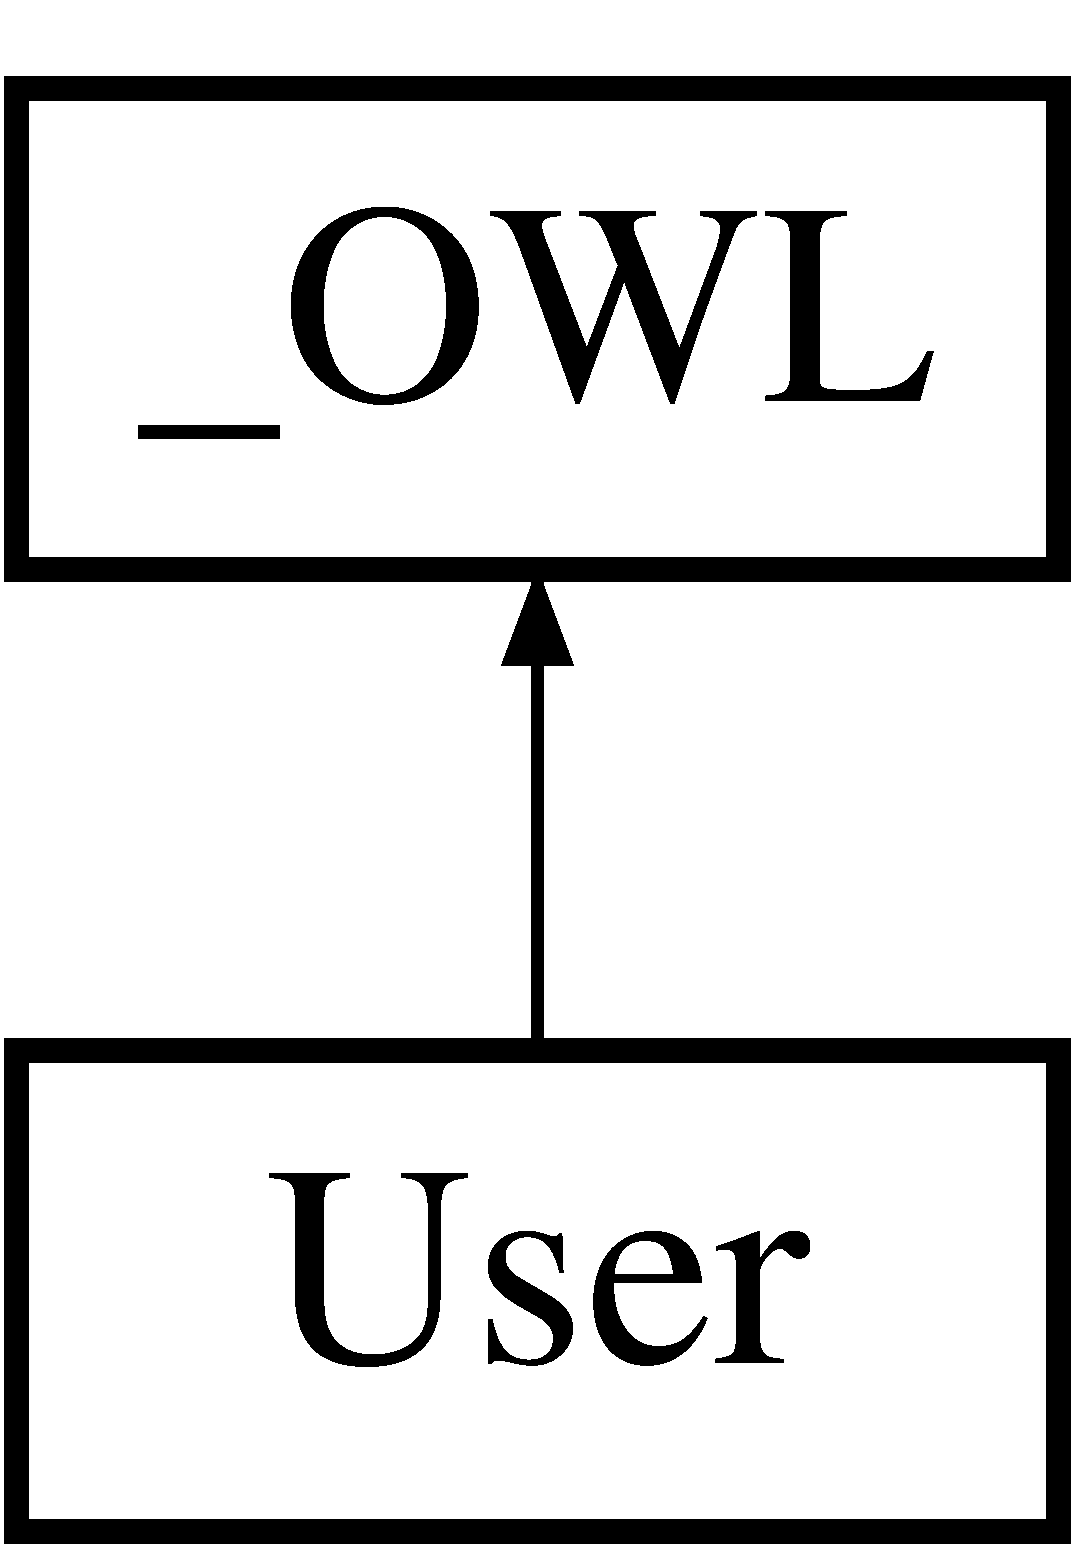
\includegraphics[height=2.000000cm]{classUser}
\end{center}
\end{figure}
\subsection*{Public Member Functions}
\begin{DoxyCompactItemize}
\item 
{\bf \_\-\_\-destruct} ()
\item 
{\bf login} (\$username, \$password)
\item 
{\bf logout} (\$reset\_\-status=true)
\item 
{\bf isLoggedIn} ()
\item 
{\bf get\_\-username} ()
\item 
{\bf get\_\-user\_\-id} ()
\item 
{\bf get\_\-session\_\-id} ()
\item 
{\bf set\_\-session\_\-var} (\$var, \$val=0, \$flg={\bf SESSIONVAR\_\-SET})
\item 
{\bf get\_\-session\_\-var} (\$var, \$default=null)
\item 
{\bf get\_\-status} ()
\item 
{\bf get\_\-severity} (\$status=null)
\item 
{\bf succeeded} (\$\_\-ok={\bf OWL\_\-SUCCESS}, \&\$\_\-object=null)
\item 
{\bf signal} (\$level={\bf OWL\_\-INFO}, \&\$text=false)
\item 
{\bf traceback} (\&\$text=false, \$depth=0)
\end{DoxyCompactItemize}
\subsection*{Static Public Member Functions}
\begin{DoxyCompactItemize}
\item 
static {\bf password\_\-strength} (\$\_\-pwd, \$\_\-compare=array())
\end{DoxyCompactItemize}
\subsection*{Protected Member Functions}
\begin{DoxyCompactItemize}
\item 
{\bf construct} (\$username=null)
\item 
{\bf register} (\$username, \$email, \$password, \$vpassword, \$group=0)
\item 
{\bf confirm} (array \$\_\-confirmation)
\item 
{\bf init} ()
\item 
{\bf set\_\-callback} (\$\_\-dispatcher)
\item 
{\bf set\_\-callback\_\-argument} (array \$\_\-arg)
\item 
{\bf get\_\-callback} ()
\item 
{\bf reset} ()
\item 
{\bf save\_\-status} ()
\item 
{\bf restore\_\-status} ()
\item 
{\bf check} (\&\$object, \$level={\bf OWL\_\-WARNING})
\item 
{\bf set\_\-status} (\$status, \$params=array())
\item 
{\bf set\_\-high\_\-severity} (\&\$object=null)
\end{DoxyCompactItemize}
\subsection*{Protected Attributes}
\begin{DoxyCompactItemize}
\item 
{\bf \$severity}
\end{DoxyCompactItemize}
\subsection*{Private Member Functions}
\begin{DoxyCompactItemize}
\item 
{\bf read\_\-userdata} ()
\item 
{\bf set\_\-username} (\$username)
\item 
{\bf hash\_\-password} (\$password)
\item 
{\bf username\_\-exists} (\$username)
\item 
{\bf get\_\-memberships} ()
\end{DoxyCompactItemize}
\subsection*{Private Attributes}
\begin{DoxyCompactItemize}
\item 
{\bf \$session}
\item 
{\bf \$dataset}
\item 
{\bf \$group}
\item 
{\bf \$memberships}
\item 
{\bf \$user\_\-data}
\item 
{\bf \$rights}
\end{DoxyCompactItemize}


\subsection{Detailed Description}
the OWL-\/PHP user object 

This class handles the \doxyref{OWL}{p.}{classOWL} users \begin{DoxyAuthor}{Author}
Oscar van Eijk, Oveas Functionality Provider 
\end{DoxyAuthor}
\begin{DoxyVersion}{Version}
Aug 27, 2008 -\/-\/ O van Eijk -\/-\/ initial version 
\end{DoxyVersion}


\subsection{Constructor \& Destructor Documentation}
\index{User@{User}!\_\-\_\-destruct@{\_\-\_\-destruct}}
\index{\_\-\_\-destruct@{\_\-\_\-destruct}!User@{User}}
\subsubsection[{\_\-\_\-destruct}]{\setlength{\rightskip}{0pt plus 5cm}User::\_\-\_\-destruct (
\begin{DoxyParamCaption}
{}
\end{DoxyParamCaption}
)}\label{classUser_accd20149a7414612c1505e022eb63ffc}
When a run ends, write the sessiondata 

Reimplemented from {\bf \_\-OWL} \doxyref{}{p.}{class__OWL_a44fd2222476a3109286cc82d92b6bbcc}.



\subsection{Member Function Documentation}
\index{User@{User}!check@{check}}
\index{check@{check}!User@{User}}
\subsubsection[{check}]{\setlength{\rightskip}{0pt plus 5cm}\_\-OWL::check (
\begin{DoxyParamCaption}
\item[{\&\$}]{object, }
\item[{\$}]{level = {\ttfamily {\bf OWL\_\-WARNING}}}
\end{DoxyParamCaption}
)\hspace{0.3cm}{\ttfamily  [protected, inherited]}}\label{class__OWL_ae2e3c56e5f3c4ce4156c6b1bb1c50f63}
This is a helper function for lazy developers. Some checks have to be made quite often, this is a kinda macro to handle that. It compares the own severity level with that of a given object. If the highest level is above a given max, a traceback and reset are performed.


\begin{DoxyParams}[1]{Parameters}
\mbox{\tt in}  & {\em \$object} & Pointer to an object to check against \\
\hline
\mbox{\tt in}  & {\em \$level} & The maximum severity level \\
\hline
\end{DoxyParams}
\begin{DoxyReturn}{Returns}
True if the severity level was correct (below the max), otherwise false 
\end{DoxyReturn}


References \_\-OWL::reset(), \_\-OWL::set\_\-high\_\-severity(), and \_\-OWL::traceback().



Referenced by SessionHandler::write().

\index{User@{User}!confirm@{confirm}}
\index{confirm@{confirm}!User@{User}}
\subsubsection[{confirm}]{\setlength{\rightskip}{0pt plus 5cm}User::confirm (
\begin{DoxyParamCaption}
\item[{array \$}]{\_\-confirmation}
\end{DoxyParamCaption}
)\hspace{0.3cm}{\ttfamily  [protected]}}\label{classUser_acbcc13f994e50ee3f562e9949f6d0638}
Confirm a user registration. 
\begin{DoxyParams}[1]{Parameters}
\mbox{\tt in}  & {\em \$\_\-confirmation} & Array that must contain at least the keys 'uid' and 'vcode' \\
\hline
\end{DoxyParams}
\begin{DoxyReturn}{Returns}
True on success, false on failure 
\end{DoxyReturn}


References \_\-OWL::set\_\-status().

\index{User@{User}!construct@{construct}}
\index{construct@{construct}!User@{User}}
\subsubsection[{construct}]{\setlength{\rightskip}{0pt plus 5cm}User::construct (
\begin{DoxyParamCaption}
\item[{\$}]{username = {\ttfamily null}}
\end{DoxyParamCaption}
)\hspace{0.3cm}{\ttfamily  [protected]}}\label{classUser_a9cf024c7e3148e45afd1bee7691ceefd}
Class constructor; create a new user environment. This is not a regular constructor, since it's up to the application to decide if this is a normal object or a singleton.


\begin{DoxyParams}[1]{Parameters}
\mbox{\tt in}  & {\em \$username} & Username when logged in. Default username is 'anonymous' \\
\hline
\end{DoxyParams}


References ConfigHandler::get(), get\_\-memberships(), get\_\-session\_\-var(), \_\-OWL::init(), read\_\-userdata(), OWLCache::set(), set\_\-session\_\-var(), set\_\-username(), and \_\-OWL::succeeded().

\index{User@{User}!get\_\-callback@{get\_\-callback}}
\index{get\_\-callback@{get\_\-callback}!User@{User}}
\subsubsection[{get\_\-callback}]{\setlength{\rightskip}{0pt plus 5cm}\_\-OWL::get\_\-callback (
\begin{DoxyParamCaption}
{}
\end{DoxyParamCaption}
)\hspace{0.3cm}{\ttfamily  [protected, inherited]}}\label{class__OWL_abded13b1c97ea6e0cfe3c68cb6bcf7a5}
Retrieve a previously set (callback) dispatcher. The (callback) dispatcher is cleared immediatly. \begin{DoxyReturn}{Returns}
The dispatcher, of null on failure. 
\end{DoxyReturn}


Reimplemented in {\bf Dispatcher} \doxyref{}{p.}{classDispatcher_af4b71fa3c4d25bab86187d9dc44182f2}.



References OWL::factory().

\index{User@{User}!get\_\-memberships@{get\_\-memberships}}
\index{get\_\-memberships@{get\_\-memberships}!User@{User}}
\subsubsection[{get\_\-memberships}]{\setlength{\rightskip}{0pt plus 5cm}User::get\_\-memberships (
\begin{DoxyParamCaption}
{}
\end{DoxyParamCaption}
)\hspace{0.3cm}{\ttfamily  [private]}}\label{classUser_a4cdf747f1bbdd0ed8cc80e9f90473dfb}
Get the list of all objects this user is member of 

References \$dataset, ConfigHandler::get(), and get\_\-user\_\-id().



Referenced by construct().

\index{User@{User}!get\_\-session\_\-id@{get\_\-session\_\-id}}
\index{get\_\-session\_\-id@{get\_\-session\_\-id}!User@{User}}
\subsubsection[{get\_\-session\_\-id}]{\setlength{\rightskip}{0pt plus 5cm}User::get\_\-session\_\-id (
\begin{DoxyParamCaption}
{}
\end{DoxyParamCaption}
)}\label{classUser_ac5f09e73bdf4f3a626cd7b06c844704f}
Return the current session ID

\begin{DoxyReturn}{Returns}
the session ID 
\end{DoxyReturn}
\index{User@{User}!get\_\-session\_\-var@{get\_\-session\_\-var}}
\index{get\_\-session\_\-var@{get\_\-session\_\-var}!User@{User}}
\subsubsection[{get\_\-session\_\-var}]{\setlength{\rightskip}{0pt plus 5cm}User::get\_\-session\_\-var (
\begin{DoxyParamCaption}
\item[{\$}]{var, }
\item[{\$}]{default = {\ttfamily null}}
\end{DoxyParamCaption}
)}\label{classUser_a84f3693077e777cc1d61b45fcecdb36c}
Get a session variable


\begin{DoxyParams}[1]{Parameters}
\mbox{\tt in}  & {\em \$var} & Variable name \\
\hline
\mbox{\tt in}  & {\em \$default} & Default value to return if the variable was not set (default null) \\
\hline
\end{DoxyParams}
\begin{DoxyReturn}{Returns}
The value from the session, null if not set 
\end{DoxyReturn}


Referenced by construct(), and get\_\-user\_\-id().

\index{User@{User}!get\_\-severity@{get\_\-severity}}
\index{get\_\-severity@{get\_\-severity}!User@{User}}
\subsubsection[{get\_\-severity}]{\setlength{\rightskip}{0pt plus 5cm}\_\-OWL::get\_\-severity (
\begin{DoxyParamCaption}
\item[{\$}]{status = {\ttfamily null}}
\end{DoxyParamCaption}
)\hspace{0.3cm}{\ttfamily  [inherited]}}\label{class__OWL_adf9509ef96858be7bdd9414c5ef129aa}
Get the current object severity level.


\begin{DoxyParams}[1]{Parameters}
\mbox{\tt in}  & {\em \$status} & An optional parameter to check an other status code i.s.o the object's current status. \\
\hline
\end{DoxyParams}
\begin{DoxyReturn}{Returns}
Status severity level 
\end{DoxyReturn}


References \_\-OWL::\$status.



Referenced by LogHandler::compose\_\-message(), LogHandler::log(), and DataHandler::set\_\-key().

\index{User@{User}!get\_\-status@{get\_\-status}}
\index{get\_\-status@{get\_\-status}!User@{User}}
\subsubsection[{get\_\-status}]{\setlength{\rightskip}{0pt plus 5cm}\_\-OWL::get\_\-status (
\begin{DoxyParamCaption}
{}
\end{DoxyParamCaption}
)\hspace{0.3cm}{\ttfamily  [final, inherited]}}\label{class__OWL_a99ec771fa2c5c279f80152cc09e489a8}
Get the current object status.

\begin{DoxyReturn}{Returns}
Object's status code 
\end{DoxyReturn}


Referenced by SchemeHandler::compare().

\index{User@{User}!get\_\-user\_\-id@{get\_\-user\_\-id}}
\index{get\_\-user\_\-id@{get\_\-user\_\-id}!User@{User}}
\subsubsection[{get\_\-user\_\-id}]{\setlength{\rightskip}{0pt plus 5cm}User::get\_\-user\_\-id (
\begin{DoxyParamCaption}
{}
\end{DoxyParamCaption}
)}\label{classUser_a17c0e323e79f0de0b19574549e6c7906}
Return the userID of the current session 

References get\_\-session\_\-var().



Referenced by get\_\-memberships().

\index{User@{User}!get\_\-username@{get\_\-username}}
\index{get\_\-username@{get\_\-username}!User@{User}}
\subsubsection[{get\_\-username}]{\setlength{\rightskip}{0pt plus 5cm}User::get\_\-username (
\begin{DoxyParamCaption}
{}
\end{DoxyParamCaption}
)}\label{classUser_a1348ddf190d4df2518665fb51305a902}
Return the username of the current session \index{User@{User}!hash\_\-password@{hash\_\-password}}
\index{hash\_\-password@{hash\_\-password}!User@{User}}
\subsubsection[{hash\_\-password}]{\setlength{\rightskip}{0pt plus 5cm}User::hash\_\-password (
\begin{DoxyParamCaption}
\item[{\$}]{password}
\end{DoxyParamCaption}
)\hspace{0.3cm}{\ttfamily  [private]}}\label{classUser_a47614112ad1835abf56dd5bc370d6388}
Encrypt a given password


\begin{DoxyParams}[1]{Parameters}
\mbox{\tt in}  & {\em \$password} & Given password in plain text format \\
\hline
\end{DoxyParams}
\begin{DoxyReturn}{Returns}
The encrypted password 
\end{DoxyReturn}


References ConfigHandler::get().



Referenced by login(), and register().

\index{User@{User}!init@{init}}
\index{init@{init}!User@{User}}
\subsubsection[{init}]{\setlength{\rightskip}{0pt plus 5cm}\_\-OWL::init (
\begin{DoxyParamCaption}
{}
\end{DoxyParamCaption}
)\hspace{0.3cm}{\ttfamily  [protected, inherited]}}\label{class__OWL_ae0ef3ded56e8a6b34b6461e5a721cd3e}
This function should be called by all constuctors. It initializes the general characteristics. Status is 'warning' by default, it's up to the contructor to set a proper status; if it's still 'warning', this $\ast$might$\ast$ indicate something went wrong. 

References OWL::factory(), and \_\-OWL::set\_\-status().



Referenced by FormFieldPlugin::\_\-\_\-construct(), Tablerow::\_\-\_\-construct(), Tablecell::\_\-\_\-construct(), Table::\_\-\_\-construct(), Document::\_\-\_\-construct(), ContainerPlugin::\_\-\_\-construct(), Container::\_\-\_\-construct(), SessionHandler::\_\-\_\-construct(), SchemeHandler::\_\-\_\-construct(), LogHandler::\_\-\_\-construct(), ImageHandler::\_\-\_\-construct(), GroupHandler::\_\-\_\-construct(), FormHandler::\_\-\_\-construct(), FileHandler::\_\-\_\-construct(), DbHandler::\_\-\_\-construct(), DataHandler::\_\-\_\-construct(), OWL::\_\-\_\-construct(), Form::\_\-\_\-construct(), Dispatcher::\_\-\_\-construct(), and construct().

\index{User@{User}!isLoggedIn@{isLoggedIn}}
\index{isLoggedIn@{isLoggedIn}!User@{User}}
\subsubsection[{isLoggedIn}]{\setlength{\rightskip}{0pt plus 5cm}User::isLoggedIn (
\begin{DoxyParamCaption}
{}
\end{DoxyParamCaption}
)}\label{classUser_ac1eeb3fabf0d0398ba60d537316c3bbe}
Check is the current user is logged in \begin{DoxyReturn}{Returns}
True when logged in 
\end{DoxyReturn}


References ConfigHandler::get().

\index{User@{User}!login@{login}}
\index{login@{login}!User@{User}}
\subsubsection[{login}]{\setlength{\rightskip}{0pt plus 5cm}User::login (
\begin{DoxyParamCaption}
\item[{\$}]{username, }
\item[{\$}]{password}
\end{DoxyParamCaption}
)}\label{classUser_a2c4fae5935ebf84e787126795bf42988}
Log in


\begin{DoxyParams}[1]{Parameters}
\mbox{\tt in}  & {\em \$username} & Given username. Might be taken from the session as well, but given as a parameter here to suppress the E\_\-STRICT Declaration warning \\
\hline
\mbox{\tt in}  & {\em \$password} & The user provided password \\
\hline
\end{DoxyParams}
\begin{DoxyReturn}{Returns}
True on success, False otherwise 
\end{DoxyReturn}


References ConfigHandler::get(), hash\_\-password(), logout(), \_\-OWL::set\_\-status(), set\_\-username(), and \_\-OWL::traceback().

\index{User@{User}!logout@{logout}}
\index{logout@{logout}!User@{User}}
\subsubsection[{logout}]{\setlength{\rightskip}{0pt plus 5cm}User::logout (
\begin{DoxyParamCaption}
\item[{\$}]{reset\_\-status = {\ttfamily true}}
\end{DoxyParamCaption}
)}\label{classUser_a95e19a7d141f922c2870a6404ff641b1}
Log out the current user Note: After logging out, the session still continues. The calling app must take care of the forward (e.g. with a header('location: ' . \$\_\-SERVER['PHP\_\-SELF']) after a call to \doxyref{User::logout()}{p.}{classUser_a95e19a7d141f922c2870a6404ff641b1}). 
\begin{DoxyParams}[1]{Parameters}
\mbox{\tt in}  & {\em \$reset\_\-status} & When true (default) the object status will be reset \\
\hline
\end{DoxyParams}


References ConfigHandler::get(), \_\-OWL::restore\_\-status(), \_\-OWL::save\_\-status(), and set\_\-username().



Referenced by login().

\index{User@{User}!password\_\-strength@{password\_\-strength}}
\index{password\_\-strength@{password\_\-strength}!User@{User}}
\subsubsection[{password\_\-strength}]{\setlength{\rightskip}{0pt plus 5cm}static User::password\_\-strength (
\begin{DoxyParamCaption}
\item[{\$}]{\_\-pwd, }
\item[{\$}]{\_\-compare = {\ttfamily array()}}
\end{DoxyParamCaption}
)\hspace{0.3cm}{\ttfamily  [static]}}\label{classUser_a4d4ea8d545686fa335e8597f1bab73d2}
Calculate the strenbgth of a given password. This method uses string length and checks for variations in the characters and digits used. 
\begin{DoxyParams}[1]{Parameters}
\mbox{\tt in}  & {\em \$\_\-pwd} & The password as a string \\
\hline
\mbox{\tt in}  & {\em \$\_\-compare} & An optional array of string to compare with, like username and or email address. If the password if (part of) any of the strings in the array, the strength is decreased. \\
\hline
\end{DoxyParams}
\begin{DoxyReturn}{Returns}
An integer from 0-\/10 indicating the strength, where 0 is the lowest and 10 the highest level 
\end{DoxyReturn}
\index{User@{User}!read\_\-userdata@{read\_\-userdata}}
\index{read\_\-userdata@{read\_\-userdata}!User@{User}}
\subsubsection[{read\_\-userdata}]{\setlength{\rightskip}{0pt plus 5cm}User::read\_\-userdata (
\begin{DoxyParamCaption}
{}
\end{DoxyParamCaption}
)\hspace{0.3cm}{\ttfamily  [private]}}\label{classUser_aafc3d11ecbdc694c094aab8630b8c768}
When a new session starts for a use that was logged in before retrieve the userdata back from the database 

References \_\-OWL::set\_\-status().



Referenced by construct().

\index{User@{User}!register@{register}}
\index{register@{register}!User@{User}}
\subsubsection[{register}]{\setlength{\rightskip}{0pt plus 5cm}User::register (
\begin{DoxyParamCaption}
\item[{\$}]{username, }
\item[{\$}]{email, }
\item[{\$}]{password, }
\item[{\$}]{vpassword, }
\item[{\$}]{group = {\ttfamily 0}}
\end{DoxyParamCaption}
)\hspace{0.3cm}{\ttfamily  [protected]}}\label{classUser_a0454a21e40da25584033f99251540ab3}
\doxyref{Register}{p.}{classRegister} a new username


\begin{DoxyParams}[1]{Parameters}
\mbox{\tt in}  & {\em \$username} & Given username \\
\hline
\mbox{\tt in}  & {\em \$email} & Given username \\
\hline
\mbox{\tt in}  & {\em \$password} & Given password \\
\hline
\mbox{\tt in}  & {\em \$vpassword} & Given password \\
\hline
\mbox{\tt in}  & {\em \$group} & Default \doxyref{Group}{p.}{classGroup} ID, defaults to the user$|$default\_\-group config setting \\
\hline
\end{DoxyParams}
\begin{DoxyReturn}{Returns}
New user ID or -\/1 on failure 
\end{DoxyReturn}


References \$group, ConfigHandler::get(), hash\_\-password(), RandomString(), \_\-OWL::set\_\-callback\_\-argument(), \_\-OWL::set\_\-status(), and username\_\-exists().

\index{User@{User}!reset@{reset}}
\index{reset@{reset}!User@{User}}
\subsubsection[{reset}]{\setlength{\rightskip}{0pt plus 5cm}\_\-OWL::reset (
\begin{DoxyParamCaption}
{}
\end{DoxyParamCaption}
)\hspace{0.3cm}{\ttfamily  [protected, inherited]}}\label{class__OWL_a2f2a042bcf31965194c03033df0edc9b}
General reset function for all objects. Should be called after each non-\/fatal error 

Reimplemented in {\bf DbHandler} \doxyref{}{p.}{classDbHandler_a9982df4830f05803935bb31bac7fae3d}, and {\bf SchemeHandler} \doxyref{}{p.}{classSchemeHandler_aa25feb4a70d67b3d571904be4b2f50bc}.



References \_\-OWL::reset\_\-calltree().



Referenced by \_\-OWL::check(), SessionHandler::read(), DataHandler::reset(), and \_\-OWL::set\_\-status().

\index{User@{User}!restore\_\-status@{restore\_\-status}}
\index{restore\_\-status@{restore\_\-status}!User@{User}}
\subsubsection[{restore\_\-status}]{\setlength{\rightskip}{0pt plus 5cm}\_\-OWL::restore\_\-status (
\begin{DoxyParamCaption}
{}
\end{DoxyParamCaption}
)\hspace{0.3cm}{\ttfamily  [protected, inherited]}}\label{class__OWL_a465eeaf40edd9f9c848841700c32ce55}
Restore the previously saved status object and destroy the copy 

References \_\-OWL::set\_\-status().



Referenced by logout().

\index{User@{User}!save\_\-status@{save\_\-status}}
\index{save\_\-status@{save\_\-status}!User@{User}}
\subsubsection[{save\_\-status}]{\setlength{\rightskip}{0pt plus 5cm}\_\-OWL::save\_\-status (
\begin{DoxyParamCaption}
{}
\end{DoxyParamCaption}
)\hspace{0.3cm}{\ttfamily  [protected, inherited]}}\label{class__OWL_a9e49b9c76fbc021b244c6915ea536d71}
Create a copy of the status object 

Referenced by logout().

\index{User@{User}!set\_\-callback@{set\_\-callback}}
\index{set\_\-callback@{set\_\-callback}!User@{User}}
\subsubsection[{set\_\-callback}]{\setlength{\rightskip}{0pt plus 5cm}\_\-OWL::set\_\-callback (
\begin{DoxyParamCaption}
\item[{\$}]{\_\-dispatcher}
\end{DoxyParamCaption}
)\hspace{0.3cm}{\ttfamily  [protected, inherited]}}\label{class__OWL_a28d9025eaf37b49d63cb334ed28c33f0}
Set a dispatcher for later callback 
\begin{DoxyParams}[1]{Parameters}
\mbox{\tt in}  & {\em \$\_\-dispatcher} & Dispatched, \\
\hline
\end{DoxyParams}
\begin{DoxySeeAlso}{See also}
\doxyref{Dispatcher::composeDispatcher()}{p.}{classDispatcher_a8a974bbbb30be7cda74f9929972fd2f6} 
\end{DoxySeeAlso}
\begin{DoxyReturn}{Returns}
True on success, false on failure 
\end{DoxyReturn}


References OWL::factory().

\index{User@{User}!set\_\-callback\_\-argument@{set\_\-callback\_\-argument}}
\index{set\_\-callback\_\-argument@{set\_\-callback\_\-argument}!User@{User}}
\subsubsection[{set\_\-callback\_\-argument}]{\setlength{\rightskip}{0pt plus 5cm}\_\-OWL::set\_\-callback\_\-argument (
\begin{DoxyParamCaption}
\item[{array \$}]{\_\-arg}
\end{DoxyParamCaption}
)\hspace{0.3cm}{\ttfamily  [protected, inherited]}}\label{class__OWL_a1e26611ce858b237f5a98a91ea3c3a1b}
Add an argument to a previously registered callback dispatcher 
\begin{DoxyParams}[1]{Parameters}
\mbox{\tt in}  & {\em \$\_\-arg} & Argument, must be an array type. When non-\/ arrays should be passed as arguments, the must be set when the callback is registered already \\
\hline
\end{DoxyParams}
\begin{DoxyReturn}{Returns}
True on success, false on failure 
\end{DoxyReturn}


References OWL::factory().



Referenced by register().

\index{User@{User}!set\_\-high\_\-severity@{set\_\-high\_\-severity}}
\index{set\_\-high\_\-severity@{set\_\-high\_\-severity}!User@{User}}
\subsubsection[{set\_\-high\_\-severity}]{\setlength{\rightskip}{0pt plus 5cm}\_\-OWL::set\_\-high\_\-severity (
\begin{DoxyParamCaption}
\item[{\&\$}]{object = {\ttfamily null}}
\end{DoxyParamCaption}
)\hspace{0.3cm}{\ttfamily  [protected, inherited]}}\label{class__OWL_a576829692a3b66e3d518853bf43abae3}
Compare the severity level of the current object with a given one and set my statuspointer to the object with the highest level. 

Referenced by \_\-OWL::check(), DataHandler::db(), DataHandler::prepare(), and SessionHandler::read().

\index{User@{User}!set\_\-session\_\-var@{set\_\-session\_\-var}}
\index{set\_\-session\_\-var@{set\_\-session\_\-var}!User@{User}}
\subsubsection[{set\_\-session\_\-var}]{\setlength{\rightskip}{0pt plus 5cm}User::set\_\-session\_\-var (
\begin{DoxyParamCaption}
\item[{\$}]{var, }
\item[{\$}]{val = {\ttfamily 0}, }
\item[{\$}]{flg = {\ttfamily {\bf SESSIONVAR\_\-SET}}}
\end{DoxyParamCaption}
)}\label{classUser_a80108765c46ddec1ab776a774ae07f53}
Set a session variable


\begin{DoxyParams}[1]{Parameters}
\mbox{\tt in}  & {\em \$var} & Variable name \\
\hline
\mbox{\tt in}  & {\em \$val} & Variable value (default 0) \\
\hline
\mbox{\tt in}  & {\em \$flg} & How to handle the value. Default SESSIONVAR\_\-SET \\
\hline
\end{DoxyParams}


Referenced by construct().

\index{User@{User}!set\_\-status@{set\_\-status}}
\index{set\_\-status@{set\_\-status}!User@{User}}
\subsubsection[{set\_\-status}]{\setlength{\rightskip}{0pt plus 5cm}\_\-OWL::set\_\-status (
\begin{DoxyParamCaption}
\item[{\$}]{status, }
\item[{\$}]{params = {\ttfamily array~()}}
\end{DoxyParamCaption}
)\hspace{0.3cm}{\ttfamily  [final, protected, inherited]}}\label{class__OWL_aea912d0ede9b3c2a69b79072d94d4787}
Set the current object status to the specified value.


\begin{DoxyParams}[1]{Parameters}
\mbox{\tt in}  & {\em \$status} & \doxyref{OWL}{p.}{classOWL} status code \\
\hline
\mbox{\tt in}  & {\em \$params} & \\
\hline
\end{DoxyParams}


References \$GLOBALS, \_\-OWL::\$status, ConfigHandler::get(), Register::get\_\-code(), \_\-OWL::reset(), and \_\-OWL::signal().



Referenced by DbHandler::\_\-\_\-clone(), Container::\_\-\_\-construct(), SchemeHandler::\_\-\_\-construct(), ImageHandler::\_\-\_\-construct(), FormHandler::\_\-\_\-construct(), FileHandler::\_\-\_\-construct(), DbHandler::\_\-\_\-construct(), DataHandler::\_\-\_\-construct(), Session::\_\-\_\-construct(), BaseElement::\_\-getContent(), Form::addField(), FormFieldRadioPlugin::addOption(), BaseElement::addToContent(), DbHandler::alt(), SchemeHandler::alter\_\-scheme(), FileHandler::close(), Dispatcher::composeDispatcher(), confirm(), DbHandler::connect(), DbHandler::create(), SchemeHandler::create\_\-scheme(), SchemeHandler::define\_\-index(), SchemeHandler::define\_\-scheme(), Dispatcher::dispatch(), FormHandler::get(), DataHandler::get(), SchemeHandler::get\_\-table\_\-columns(), SchemeHandler::get\_\-table\_\-indexes(), \_\-OWL::init(), Document::loadScript(), Document::loadStyle(), login(), FileHandler::open(), DbHandler::open(), LogHandler::open\_\-logfile(), DataHandler::prepare(), DbHandler::prepare\_\-delete(), DbHandler::prepare\_\-field(), DbHandler::prepare\_\-insert(), DbHandler::prepare\_\-read(), DbHandler::prepare\_\-update(), DbHandler::read(), FileHandler::read\_\-line(), read\_\-userdata(), register(), Dispatcher::register\_\-argument(), Dispatcher::register\_\-callback(), \_\-OWL::restore\_\-status(), SchemeHandler::scheme(), FormHandler::set(), DataHandler::set\_\-join(), DataHandler::set\_\-key(), BaseElement::setAttributes(), BaseElement::setContent(), Form::setEncoding(), Document::setFavicon(), Form::setFieldAttributes(), FormFieldTextPlugin::setMaxsize(), Document::setMeta(), Form::setMethod(), FormFieldRadioPlugin::setSelected(), FormFieldTextPlugin::setSize(), FormFieldSelectPlugin::setSize(), FormFieldSelectPlugin::setValue(), Form::showField(), SchemeHandler::table\_\-description(), SchemeHandler::validate\_\-scheme(), and DbHandler::write().

\index{User@{User}!set\_\-username@{set\_\-username}}
\index{set\_\-username@{set\_\-username}!User@{User}}
\subsubsection[{set\_\-username}]{\setlength{\rightskip}{0pt plus 5cm}User::set\_\-username (
\begin{DoxyParamCaption}
\item[{\$}]{username}
\end{DoxyParamCaption}
)\hspace{0.3cm}{\ttfamily  [private]}}\label{classUser_ab7574963efcbb5acbc71d7ba97c50b68}
Set the username 
\begin{DoxyParams}[1]{Parameters}
\mbox{\tt in}  & {\em \$username} & Username \\
\hline
\end{DoxyParams}


References ConfigHandler::get().



Referenced by construct(), login(), and logout().

\index{User@{User}!signal@{signal}}
\index{signal@{signal}!User@{User}}
\subsubsection[{signal}]{\setlength{\rightskip}{0pt plus 5cm}\_\-OWL::signal (
\begin{DoxyParamCaption}
\item[{\$}]{level = {\ttfamily {\bf OWL\_\-INFO}}, }
\item[{\&\$}]{text = {\ttfamily false}}
\end{DoxyParamCaption}
)\hspace{0.3cm}{\ttfamily  [inherited]}}\label{class__OWL_a51ba4a16409acf2a2f61f286939091a5}
Display the message for the current object status


\begin{DoxyParams}[1]{Parameters}
\mbox{\tt in}  & {\em \$level} & An optional severity level; message will only be displayed when it is at least of this level. \\
\hline
\mbox{\tt out}  & {\em \$text} & If this parameter is given, the message text is returned in this string instead of echood. \\
\hline
\end{DoxyParams}
\begin{DoxyReturn}{Returns}
The severity level for this object 
\end{DoxyReturn}


References ConfigHandler::get().



Referenced by \_\-OWL::set\_\-status(), and \_\-OWL::traceback().

\index{User@{User}!succeeded@{succeeded}}
\index{succeeded@{succeeded}!User@{User}}
\subsubsection[{succeeded}]{\setlength{\rightskip}{0pt plus 5cm}\_\-OWL::succeeded (
\begin{DoxyParamCaption}
\item[{\$}]{\_\-ok = {\ttfamily {\bf OWL\_\-SUCCESS}}, }
\item[{\&\$}]{\_\-object = {\ttfamily null}}
\end{DoxyParamCaption}
)\hspace{0.3cm}{\ttfamily  [inherited]}}\label{class__OWL_a53ab4d3bbb2c6a56966c339ca4b4c805}
Check if the object currenlty has a success state 
\begin{DoxyParams}[1]{Parameters}
\mbox{\tt in}  & {\em \$\_\-ok} & The highest severity that's considered successfull, default OWL\_\-SUCCESS \\
\hline
\mbox{\tt in}  & {\em \$\_\-object} & REference to the object to check, defaults to the current object \\
\hline
\end{DoxyParams}
\begin{DoxyReturn}{Returns}
Boolean true when successfull 
\end{DoxyReturn}


Referenced by construct(), Dispatcher::register\_\-argument(), and Dispatcher::register\_\-callback().

\index{User@{User}!traceback@{traceback}}
\index{traceback@{traceback}!User@{User}}
\subsubsection[{traceback}]{\setlength{\rightskip}{0pt plus 5cm}\_\-OWL::traceback (
\begin{DoxyParamCaption}
\item[{\&\$}]{text = {\ttfamily false}, }
\item[{\$}]{depth = {\ttfamily 0}}
\end{DoxyParamCaption}
)\hspace{0.3cm}{\ttfamily  [inherited]}}\label{class__OWL_aa29547995d6741b7d2b90c1d4ea99a13}
If somehwere in the nested calls an error occured, we can traceback the original failing object with this function and signal the message.


\begin{DoxyParams}[1]{Parameters}
\mbox{\tt out}  & {\em \$text} & Optional variable in which the message text can be stored. If not given, the text will be written to standard output \\
\hline
\mbox{\tt in}  & {\em \$depth} & This paramater should be initially empty. It calculates the depth in recursive calls. \\
\hline
\end{DoxyParams}
\begin{DoxyReturn}{Returns}
Severity code of the failing object 
\end{DoxyReturn}


References \_\-OWL::signal().



Referenced by \_\-OWL::check(), login(), and SessionHandler::read().

\index{User@{User}!username\_\-exists@{username\_\-exists}}
\index{username\_\-exists@{username\_\-exists}!User@{User}}
\subsubsection[{username\_\-exists}]{\setlength{\rightskip}{0pt plus 5cm}User::username\_\-exists (
\begin{DoxyParamCaption}
\item[{\$}]{username}
\end{DoxyParamCaption}
)\hspace{0.3cm}{\ttfamily  [private]}}\label{classUser_acc22035525b91a78b1b8e088393b707a}
Check is a given username exists 
\begin{DoxyParams}[1]{Parameters}
\mbox{\tt in}  & {\em \$username} & The username to check \\
\hline
\end{DoxyParams}
\begin{DoxyReturn}{Returns}
True when the username exists false otherwise 
\end{DoxyReturn}


Referenced by register().



\subsection{Member Data Documentation}
\index{User@{User}!\$dataset@{\$dataset}}
\index{\$dataset@{\$dataset}!User@{User}}
\subsubsection[{\$dataset}]{\setlength{\rightskip}{0pt plus 5cm}User::\$dataset\hspace{0.3cm}{\ttfamily  [private]}}\label{classUser_ac516c03e30e262e4085151df30109b00}
Link to a datahandler object. This dataset is used as an interface to all database IO. 

Referenced by get\_\-memberships().

\index{User@{User}!\$group@{\$group}}
\index{\$group@{\$group}!User@{User}}
\subsubsection[{\$group}]{\setlength{\rightskip}{0pt plus 5cm}User::\$group\hspace{0.3cm}{\ttfamily  [private]}}\label{classUser_a669fa9bfc33707ca3ee6102249acaf6f}
Primary group object 

Referenced by register().

\index{User@{User}!\$memberships@{\$memberships}}
\index{\$memberships@{\$memberships}!User@{User}}
\subsubsection[{\$memberships}]{\setlength{\rightskip}{0pt plus 5cm}User::\$memberships\hspace{0.3cm}{\ttfamily  [private]}}\label{classUser_a1a8f6207b6403f4806051f82b594e2eb}
Array with the group objects the user is member of \index{User@{User}!\$rights@{\$rights}}
\index{\$rights@{\$rights}!User@{User}}
\subsubsection[{\$rights}]{\setlength{\rightskip}{0pt plus 5cm}User::\$rights\hspace{0.3cm}{\ttfamily  [private]}}\label{classUser_a3f482d6b1f02d4024e66abdb86bd1cf8}
This users rightslist \index{User@{User}!\$session@{\$session}}
\index{\$session@{\$session}!User@{User}}
\subsubsection[{\$session}]{\setlength{\rightskip}{0pt plus 5cm}User::\$session\hspace{0.3cm}{\ttfamily  [private]}}\label{classUser_a0bcbaf8fe088e8359201c8fee8cd368e}
The PHP session object \index{User@{User}!\$severity@{\$severity}}
\index{\$severity@{\$severity}!User@{User}}
\subsubsection[{\$severity}]{\setlength{\rightskip}{0pt plus 5cm}\_\-OWL::\$severity\hspace{0.3cm}{\ttfamily  [protected, inherited]}}\label{class__OWL_ad26b40a9dbbacb33e299b17826f8327c}
Severity level of the current object status \index{User@{User}!\$user\_\-data@{\$user\_\-data}}
\index{\$user\_\-data@{\$user\_\-data}!User@{User}}
\subsubsection[{\$user\_\-data}]{\setlength{\rightskip}{0pt plus 5cm}User::\$user\_\-data\hspace{0.3cm}{\ttfamily  [private]}}\label{classUser_a214012afca3e92dfeed14a9a1f80a268}
An indexed array with the user information as take from the database 

The documentation for this class was generated from the following file:\begin{DoxyCompactItemize}
\item 
/home/oscar/projects/owl-\/php/src/kernel/bo/{\bf class.user.php}\end{DoxyCompactItemize}

\section{UserHandler Class Reference}
\label{classUserHandler}\index{UserHandler@{UserHandler}}


the user object  




Inheritance diagram for UserHandler:\nopagebreak
\begin{figure}[H]
\begin{center}
\leavevmode
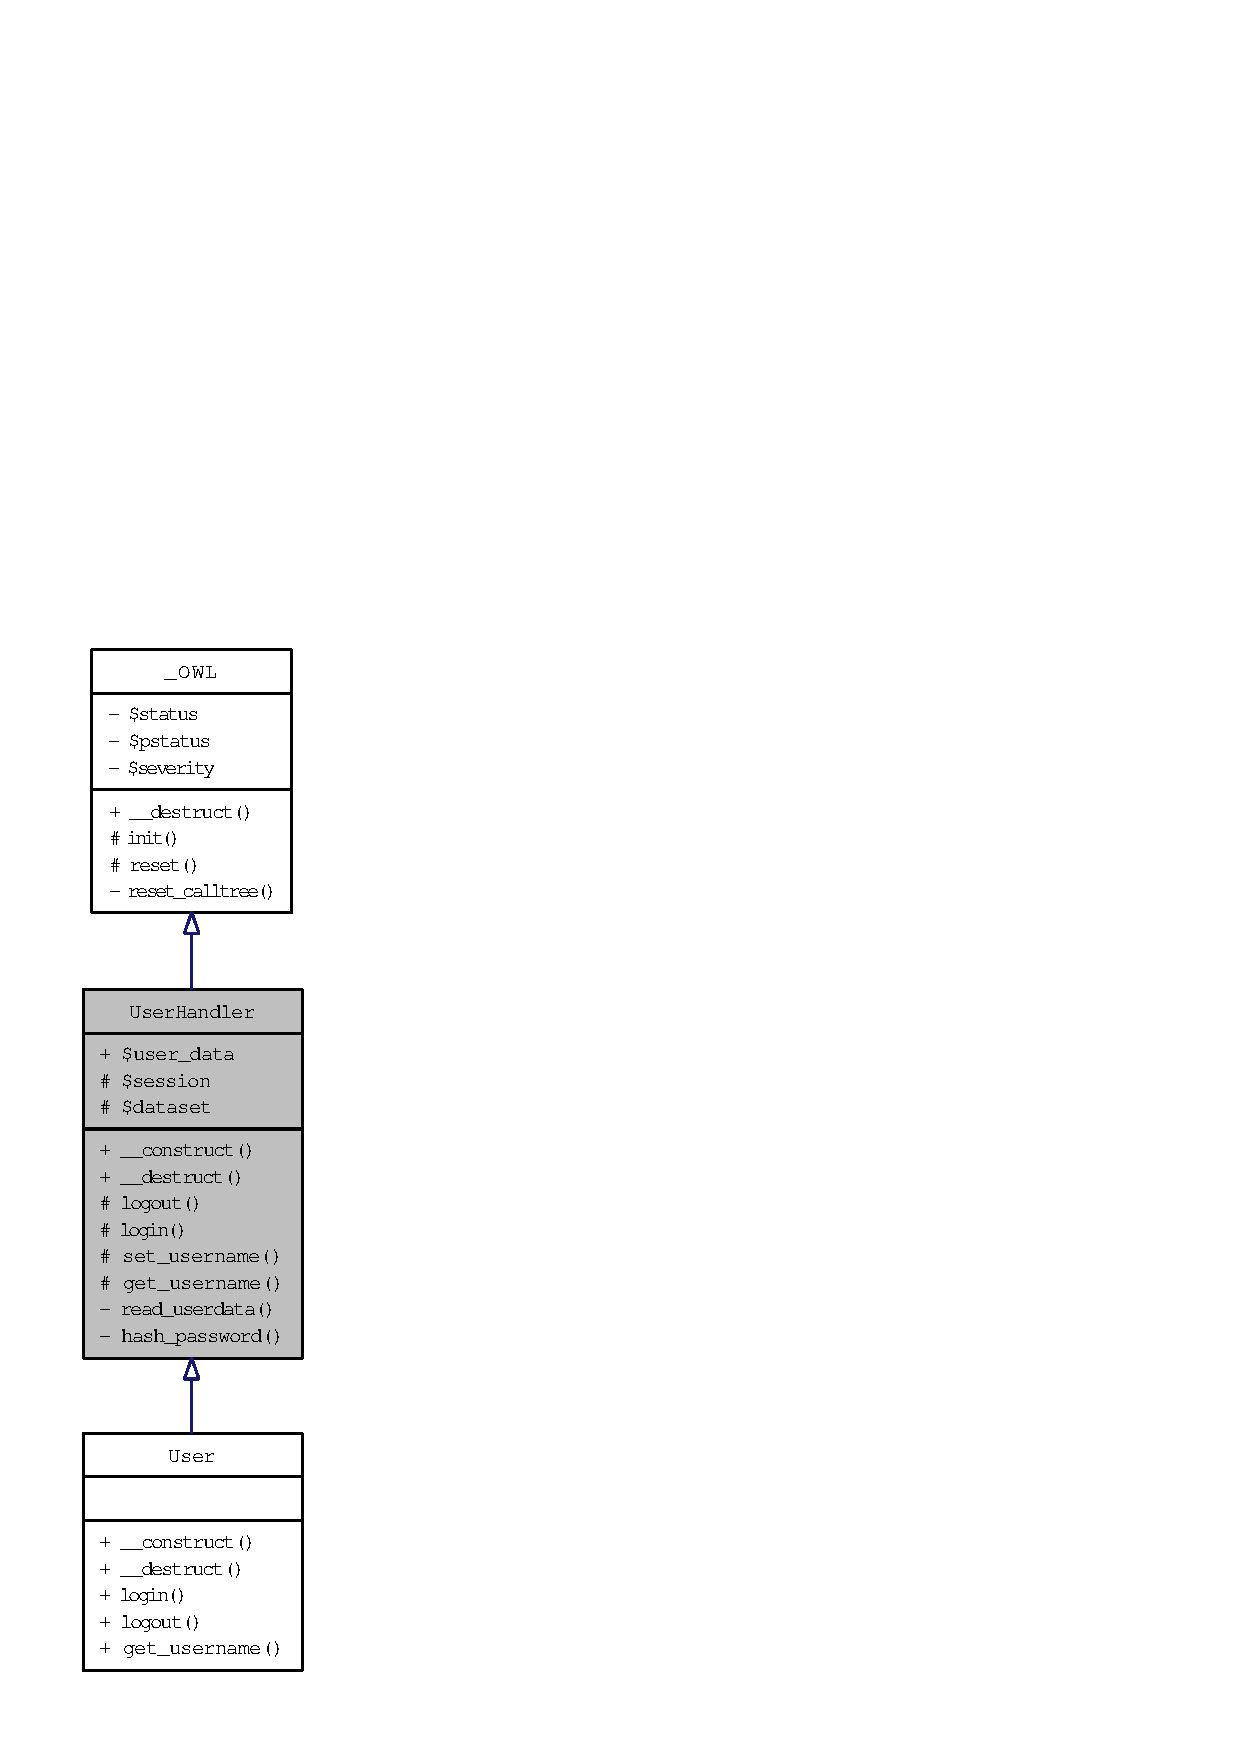
\includegraphics[height=600pt]{classUserHandler__inherit__graph}
\end{center}
\end{figure}


Collaboration diagram for UserHandler:\nopagebreak
\begin{figure}[H]
\begin{center}
\leavevmode
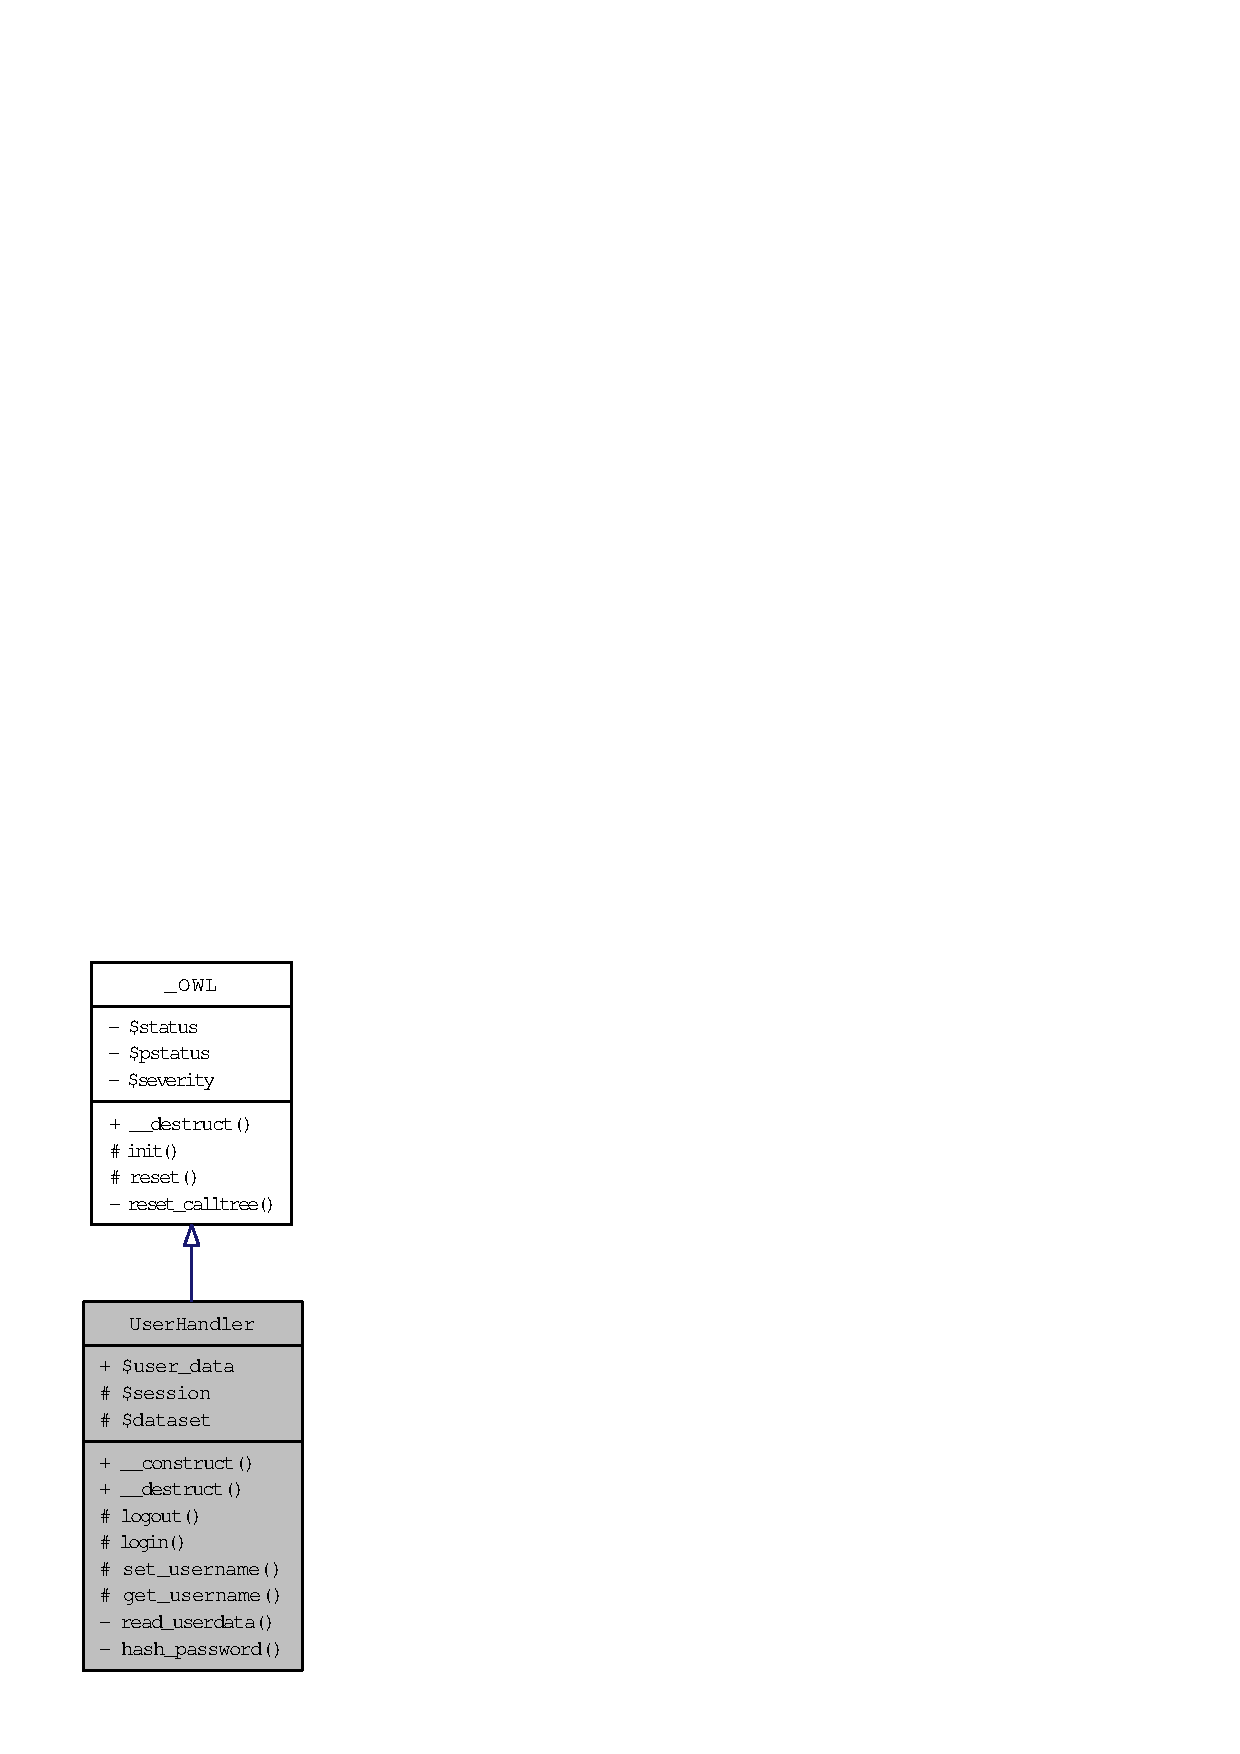
\includegraphics[width=150pt]{classUserHandler__coll__graph}
\end{center}
\end{figure}
\subsection*{Public Member Functions}
\begin{DoxyCompactItemize}
\item 
\hyperlink{classUserHandler_a624054e9693139a3fe5af0ef3b757f04}{\_\-\_\-construct} (\$username)
\item 
\hyperlink{classUserHandler_a4539c12ed2ce12a9147d61496854d5ab}{isLoggedIn} ()
\item 
\hyperlink{classUserHandler_a3e1f6381ed79caf6e1a255fb0a9cc386}{\_\-\_\-destruct} ()
\item 
\hyperlink{class__OWL_a99ec771fa2c5c279f80152cc09e489a8}{get\_\-status} ()
\item 
\hyperlink{class__OWL_adf9509ef96858be7bdd9414c5ef129aa}{get\_\-severity} (\$status=null)
\item 
\hyperlink{class__OWL_a51ba4a16409acf2a2f61f286939091a5}{signal} (\$level=\hyperlink{owl_8severitycodes_8php_a139328861128689f2f4def6a399d9057}{OWL\_\-INFO}, \&\$text=false)
\item 
\hyperlink{class__OWL_aa29547995d6741b7d2b90c1d4ea99a13}{traceback} (\&\$text=false, \$depth=0)
\end{DoxyCompactItemize}
\subsection*{Public Attributes}
\begin{DoxyCompactItemize}
\item 
\hyperlink{classUserHandler_ae7a2d59eee65560ac96b860e828bb445}{\$user\_\-data}
\end{DoxyCompactItemize}
\subsection*{Protected Member Functions}
\begin{DoxyCompactItemize}
\item 
\hyperlink{classUserHandler_a0bcf46a5b0c4a5b495cba98b8da02b7b}{logout} (\$reset\_\-status)
\item 
\hyperlink{classUserHandler_abf6562660ee8ec1663afe08550a63643}{login} (\$username, \$password)
\item 
\hyperlink{classUserHandler_afbcc9a275b547cca0bd4cff567b054a0}{set\_\-username} (\$username)
\item 
\hyperlink{classUserHandler_a76e8c8b88c8d92f2d03645e810b9253c}{get\_\-username} ()
\item 
\hyperlink{class__OWL_ae0ef3ded56e8a6b34b6461e5a721cd3e}{init} ()
\item 
\hyperlink{class__OWL_a2f2a042bcf31965194c03033df0edc9b}{reset} ()
\item 
\hyperlink{class__OWL_a9e49b9c76fbc021b244c6915ea536d71}{save\_\-status} ()
\item 
\hyperlink{class__OWL_a465eeaf40edd9f9c848841700c32ce55}{restore\_\-status} ()
\item 
\hyperlink{class__OWL_ad6f4f6946f40199dd0333cf219fa500e}{check} (\&\$object, \$level)
\item 
\hyperlink{class__OWL_aea912d0ede9b3c2a69b79072d94d4787}{set\_\-status} (\$status, \$params=array())
\item 
\hyperlink{class__OWL_a576829692a3b66e3d518853bf43abae3}{set\_\-high\_\-severity} (\&\$object=null)
\end{DoxyCompactItemize}
\subsection*{Protected Attributes}
\begin{DoxyCompactItemize}
\item 
\hyperlink{classUserHandler_af097b7fd1ee085b46a6c34e071508a7f}{\$session}
\item 
\hyperlink{classUserHandler_ac38c1ea50b2820ed03781bdbe8eb2e08}{\$dataset}
\item 
\hyperlink{class__OWL_ad26b40a9dbbacb33e299b17826f8327c}{\$severity}
\end{DoxyCompactItemize}
\subsection*{Private Member Functions}
\begin{DoxyCompactItemize}
\item 
\hyperlink{classUserHandler_a4e9fb2f7763124ea84ebaf3b744d2d88}{read\_\-userdata} ()
\item 
\hyperlink{classUserHandler_a6b2bbbdb4f1a08578c219a933880a1de}{hash\_\-password} (\$password)
\end{DoxyCompactItemize}


\subsection{Detailed Description}
the user object This class creates user sessions and handles logging in and out \begin{DoxyAuthor}{Author}
Oscar van Eijk, Oveas Functionality Provider 
\end{DoxyAuthor}
\begin{DoxyVersion}{Version}
Aug 27, 2008 -\/-\/ O van Eijk -\/-\/ initial version 
\end{DoxyVersion}


\subsection{Constructor \& Destructor Documentation}
\index{UserHandler@{UserHandler}!\_\-\_\-construct@{\_\-\_\-construct}}
\index{\_\-\_\-construct@{\_\-\_\-construct}!UserHandler@{UserHandler}}
\subsubsection[{\_\-\_\-construct}]{\setlength{\rightskip}{0pt plus 5cm}UserHandler::\_\-\_\-construct (
\begin{DoxyParamCaption}
\item[{\$}]{ username}
\end{DoxyParamCaption}
)}\label{classUserHandler_a624054e9693139a3fe5af0ef3b757f04}
Class constructor; setup the user environment


\begin{DoxyParams}{Parameters}
\item[\mbox{\tt[in]} {\em \$username}]Username. \end{DoxyParams}


Reimplemented in \hyperlink{classUser_ab8a717f17626301cc8b7815a43ea5b5b}{User}.



References ConfigHandler::get(), \_\-OWL::init(), read\_\-userdata(), \_\-OWL::set\_\-status(), and set\_\-username().

\index{UserHandler@{UserHandler}!\_\-\_\-destruct@{\_\-\_\-destruct}}
\index{\_\-\_\-destruct@{\_\-\_\-destruct}!UserHandler@{UserHandler}}
\subsubsection[{\_\-\_\-destruct}]{\setlength{\rightskip}{0pt plus 5cm}UserHandler::\_\-\_\-destruct (
\begin{DoxyParamCaption}
{}
\end{DoxyParamCaption}
)}\label{classUserHandler_a3e1f6381ed79caf6e1a255fb0a9cc386}
Class destructor 

Reimplemented from \hyperlink{class__OWL_a44fd2222476a3109286cc82d92b6bbcc}{\_\-OWL}.



Reimplemented in \hyperlink{classUser_accd20149a7414612c1505e022eb63ffc}{User}.



\subsection{Member Function Documentation}
\index{UserHandler@{UserHandler}!check@{check}}
\index{check@{check}!UserHandler@{UserHandler}}
\subsubsection[{check}]{\setlength{\rightskip}{0pt plus 5cm}\_\-OWL::check (
\begin{DoxyParamCaption}
\item[{\&\$}]{ object, }
\item[{\$}]{ level}
\end{DoxyParamCaption}
)\hspace{0.3cm}{\ttfamily  \mbox{[}protected, inherited\mbox{]}}}\label{class__OWL_ad6f4f6946f40199dd0333cf219fa500e}
This is a helper function for lazy developers. Some checks have to be made quite often, this is a kinda macro to handle that. It compares the own severity level with that of a given object. If the highest level is above a given max, a traceback and reset are performed.


\begin{DoxyParams}{Parameters}
\item[\mbox{\tt[in]} {\em \$object}]Pointer to an object to check against \item[\mbox{\tt[in]} {\em \$level}]The maximum severity level \end{DoxyParams}
\begin{DoxyReturn}{Returns}
True if the severity level was correct ( below the max), otherwise false 
\end{DoxyReturn}


References \_\-OWL::reset(), \_\-OWL::set\_\-high\_\-severity(), and \_\-OWL::traceback().



Referenced by SessionHandler::write().

\index{UserHandler@{UserHandler}!get\_\-severity@{get\_\-severity}}
\index{get\_\-severity@{get\_\-severity}!UserHandler@{UserHandler}}
\subsubsection[{get\_\-severity}]{\setlength{\rightskip}{0pt plus 5cm}\_\-OWL::get\_\-severity (
\begin{DoxyParamCaption}
\item[{\$}]{ status = {\ttfamily null}}
\end{DoxyParamCaption}
)\hspace{0.3cm}{\ttfamily  \mbox{[}inherited\mbox{]}}}\label{class__OWL_adf9509ef96858be7bdd9414c5ef129aa}
Get the current object severity level.


\begin{DoxyParams}{Parameters}
\item[\mbox{\tt[in]} {\em \$status}]An optional parameter to check an other status code i.s.o the object's current status. \end{DoxyParams}
\begin{DoxyReturn}{Returns}
Status severity level 
\end{DoxyReturn}


References \_\-OWL::\$status.



Referenced by LogHandler::compose\_\-message(), LogHandler::log(), and DataHandler::set\_\-key().

\index{UserHandler@{UserHandler}!get\_\-status@{get\_\-status}}
\index{get\_\-status@{get\_\-status}!UserHandler@{UserHandler}}
\subsubsection[{get\_\-status}]{\setlength{\rightskip}{0pt plus 5cm}\_\-OWL::get\_\-status (
\begin{DoxyParamCaption}
{}
\end{DoxyParamCaption}
)\hspace{0.3cm}{\ttfamily  \mbox{[}final, inherited\mbox{]}}}\label{class__OWL_a99ec771fa2c5c279f80152cc09e489a8}
Get the current object status.

\begin{DoxyReturn}{Returns}
Object's status code 
\end{DoxyReturn}


Referenced by SchemeHandler::compare().

\index{UserHandler@{UserHandler}!get\_\-username@{get\_\-username}}
\index{get\_\-username@{get\_\-username}!UserHandler@{UserHandler}}
\subsubsection[{get\_\-username}]{\setlength{\rightskip}{0pt plus 5cm}UserHandler::get\_\-username (
\begin{DoxyParamCaption}
{}
\end{DoxyParamCaption}
)\hspace{0.3cm}{\ttfamily  \mbox{[}protected\mbox{]}}}\label{classUserHandler_a76e8c8b88c8d92f2d03645e810b9253c}
Return the username of the current session 

Reimplemented in \hyperlink{classUser_a1348ddf190d4df2518665fb51305a902}{User}.

\index{UserHandler@{UserHandler}!hash\_\-password@{hash\_\-password}}
\index{hash\_\-password@{hash\_\-password}!UserHandler@{UserHandler}}
\subsubsection[{hash\_\-password}]{\setlength{\rightskip}{0pt plus 5cm}UserHandler::hash\_\-password (
\begin{DoxyParamCaption}
\item[{\$}]{ password}
\end{DoxyParamCaption}
)\hspace{0.3cm}{\ttfamily  \mbox{[}private\mbox{]}}}\label{classUserHandler_a6b2bbbdb4f1a08578c219a933880a1de}
Encrypt a given password


\begin{DoxyParams}{Parameters}
\item[\mbox{\tt[in]} {\em \$password}]Given password in plain text format \end{DoxyParams}
\begin{DoxyReturn}{Returns}
The encrypted password 
\end{DoxyReturn}


References ConfigHandler::get().



Referenced by login().

\index{UserHandler@{UserHandler}!init@{init}}
\index{init@{init}!UserHandler@{UserHandler}}
\subsubsection[{init}]{\setlength{\rightskip}{0pt plus 5cm}\_\-OWL::init (
\begin{DoxyParamCaption}
{}
\end{DoxyParamCaption}
)\hspace{0.3cm}{\ttfamily  \mbox{[}protected, inherited\mbox{]}}}\label{class__OWL_ae0ef3ded56e8a6b34b6461e5a721cd3e}
This function should be called by all constuctors. It initializes the general characteristics. Status is 'warning' by default, it's up to the contructor to set a proper status; if it's still 'warning', this $\ast$might$\ast$ indicate something went wrong. 

References OWL::factory().



Referenced by FormFieldPlugin::\_\-\_\-construct(), Tablerow::\_\-\_\-construct(), Tablecell::\_\-\_\-construct(), Table::\_\-\_\-construct(), Document::\_\-\_\-construct(), ContainerPlugin::\_\-\_\-construct(), Container::\_\-\_\-construct(), \_\-\_\-construct(), SessionHandler::\_\-\_\-construct(), SchemeHandler::\_\-\_\-construct(), LogHandler::\_\-\_\-construct(), ImageHandler::\_\-\_\-construct(), FormHandler::\_\-\_\-construct(), FileHandler::\_\-\_\-construct(), DbHandler::\_\-\_\-construct(), DataHandler::\_\-\_\-construct(), OWL::\_\-\_\-construct(), Form::\_\-\_\-construct(), and Dispatcher::\_\-\_\-construct().

\index{UserHandler@{UserHandler}!isLoggedIn@{isLoggedIn}}
\index{isLoggedIn@{isLoggedIn}!UserHandler@{UserHandler}}
\subsubsection[{isLoggedIn}]{\setlength{\rightskip}{0pt plus 5cm}UserHandler::isLoggedIn (
\begin{DoxyParamCaption}
{}
\end{DoxyParamCaption}
)}\label{classUserHandler_a4539c12ed2ce12a9147d61496854d5ab}


References ConfigHandler::get().

\index{UserHandler@{UserHandler}!login@{login}}
\index{login@{login}!UserHandler@{UserHandler}}
\subsubsection[{login}]{\setlength{\rightskip}{0pt plus 5cm}UserHandler::login (
\begin{DoxyParamCaption}
\item[{\$}]{ username, }
\item[{\$}]{ password}
\end{DoxyParamCaption}
)\hspace{0.3cm}{\ttfamily  \mbox{[}protected\mbox{]}}}\label{classUserHandler_abf6562660ee8ec1663afe08550a63643}
Attempt to log in with the current user and the given password


\begin{DoxyParams}{Parameters}
\item[\mbox{\tt[in]} {\em \$username}]Given username. Might be taken from the session as well, but given as a parameter here to suppress the E\_\-STRICT Declaration warning \item[\mbox{\tt[in]} {\em \$password}]The user provided password \end{DoxyParams}
\begin{DoxyReturn}{Returns}
True on success, False otherwise 
\end{DoxyReturn}


Reimplemented in \hyperlink{classUser_a2c4fae5935ebf84e787126795bf42988}{User}.



References ConfigHandler::get(), hash\_\-password(), \_\-OWL::set\_\-status(), set\_\-username(), and \_\-OWL::traceback().

\index{UserHandler@{UserHandler}!logout@{logout}}
\index{logout@{logout}!UserHandler@{UserHandler}}
\subsubsection[{logout}]{\setlength{\rightskip}{0pt plus 5cm}UserHandler::logout (
\begin{DoxyParamCaption}
\item[{\$}]{ reset\_\-status}
\end{DoxyParamCaption}
)\hspace{0.3cm}{\ttfamily  \mbox{[}protected\mbox{]}}}\label{classUserHandler_a0bcf46a5b0c4a5b495cba98b8da02b7b}
Log out the current user. 
\begin{DoxyParams}{Parameters}
\item[\mbox{\tt[in]} {\em \$reset\_\-status}]When true, the object status will be reset \end{DoxyParams}


Reimplemented in \hyperlink{classUser_a95e19a7d141f922c2870a6404ff641b1}{User}.



References \_\-OWL::restore\_\-status(), and \_\-OWL::save\_\-status().

\index{UserHandler@{UserHandler}!read\_\-userdata@{read\_\-userdata}}
\index{read\_\-userdata@{read\_\-userdata}!UserHandler@{UserHandler}}
\subsubsection[{read\_\-userdata}]{\setlength{\rightskip}{0pt plus 5cm}UserHandler::read\_\-userdata (
\begin{DoxyParamCaption}
{}
\end{DoxyParamCaption}
)\hspace{0.3cm}{\ttfamily  \mbox{[}private\mbox{]}}}\label{classUserHandler_a4e9fb2f7763124ea84ebaf3b744d2d88}
When a new session starts for a use that was logged in before retrieve the userdata back from the database 

References \_\-OWL::set\_\-status().



Referenced by \_\-\_\-construct().

\index{UserHandler@{UserHandler}!reset@{reset}}
\index{reset@{reset}!UserHandler@{UserHandler}}
\subsubsection[{reset}]{\setlength{\rightskip}{0pt plus 5cm}\_\-OWL::reset (
\begin{DoxyParamCaption}
{}
\end{DoxyParamCaption}
)\hspace{0.3cm}{\ttfamily  \mbox{[}protected, inherited\mbox{]}}}\label{class__OWL_a2f2a042bcf31965194c03033df0edc9b}
General reset function for all objects. Should be called after each non-\/fatal error 

Reimplemented in \hyperlink{classDbHandler_a9982df4830f05803935bb31bac7fae3d}{DbHandler}, and \hyperlink{classSchemeHandler_aa25feb4a70d67b3d571904be4b2f50bc}{SchemeHandler}.



References \_\-OWL::reset\_\-calltree().



Referenced by \_\-OWL::check(), SessionHandler::read(), DataHandler::reset(), and \_\-OWL::set\_\-status().

\index{UserHandler@{UserHandler}!restore\_\-status@{restore\_\-status}}
\index{restore\_\-status@{restore\_\-status}!UserHandler@{UserHandler}}
\subsubsection[{restore\_\-status}]{\setlength{\rightskip}{0pt plus 5cm}\_\-OWL::restore\_\-status (
\begin{DoxyParamCaption}
{}
\end{DoxyParamCaption}
)\hspace{0.3cm}{\ttfamily  \mbox{[}protected, inherited\mbox{]}}}\label{class__OWL_a465eeaf40edd9f9c848841700c32ce55}
Restore the previously saved status object and destroy the copy 

References \_\-OWL::set\_\-status().



Referenced by logout().

\index{UserHandler@{UserHandler}!save\_\-status@{save\_\-status}}
\index{save\_\-status@{save\_\-status}!UserHandler@{UserHandler}}
\subsubsection[{save\_\-status}]{\setlength{\rightskip}{0pt plus 5cm}\_\-OWL::save\_\-status (
\begin{DoxyParamCaption}
{}
\end{DoxyParamCaption}
)\hspace{0.3cm}{\ttfamily  \mbox{[}protected, inherited\mbox{]}}}\label{class__OWL_a9e49b9c76fbc021b244c6915ea536d71}
Create a copy of the status object 

Referenced by logout().

\index{UserHandler@{UserHandler}!set\_\-high\_\-severity@{set\_\-high\_\-severity}}
\index{set\_\-high\_\-severity@{set\_\-high\_\-severity}!UserHandler@{UserHandler}}
\subsubsection[{set\_\-high\_\-severity}]{\setlength{\rightskip}{0pt plus 5cm}\_\-OWL::set\_\-high\_\-severity (
\begin{DoxyParamCaption}
\item[{\&\$}]{ object = {\ttfamily null}}
\end{DoxyParamCaption}
)\hspace{0.3cm}{\ttfamily  \mbox{[}protected, inherited\mbox{]}}}\label{class__OWL_a576829692a3b66e3d518853bf43abae3}
Compare the severity level of the current object with a given one and set my statuspointer to the object with the highest level. 

Referenced by \_\-OWL::check(), DataHandler::db(), DataHandler::prepare(), and SessionHandler::read().

\index{UserHandler@{UserHandler}!set\_\-status@{set\_\-status}}
\index{set\_\-status@{set\_\-status}!UserHandler@{UserHandler}}
\subsubsection[{set\_\-status}]{\setlength{\rightskip}{0pt plus 5cm}\_\-OWL::set\_\-status (
\begin{DoxyParamCaption}
\item[{\$}]{ status, }
\item[{\$}]{ params = {\ttfamily array~()}}
\end{DoxyParamCaption}
)\hspace{0.3cm}{\ttfamily  \mbox{[}final, protected, inherited\mbox{]}}}\label{class__OWL_aea912d0ede9b3c2a69b79072d94d4787}
Set the current object status to the specified value.


\begin{DoxyParams}{Parameters}
\item[\mbox{\tt[in]} {\em \$status}]\hyperlink{classOWL}{OWL} status code \item[\mbox{\tt[in]} {\em \$params}]\end{DoxyParams}


References \$GLOBALS, \_\-OWL::\$status, ConfigHandler::get(), Register::get\_\-code(), \_\-OWL::reset(), and \_\-OWL::signal().



Referenced by Container::\_\-\_\-construct(), \_\-\_\-construct(), SessionHandler::\_\-\_\-construct(), SchemeHandler::\_\-\_\-construct(), ImageHandler::\_\-\_\-construct(), FormHandler::\_\-\_\-construct(), FileHandler::\_\-\_\-construct(), DbHandler::\_\-\_\-construct(), DataHandler::\_\-\_\-construct(), Form::\_\-\_\-construct(), BaseElement::\_\-getContent(), Form::addField(), FormFieldRadioPlugin::addOption(), BaseElement::addToContent(), DbHandler::alt(), SchemeHandler::alter\_\-scheme(), FileHandler::close(), DbHandler::connect(), DbHandler::create(), SchemeHandler::create\_\-scheme(), SchemeHandler::define\_\-index(), SchemeHandler::define\_\-scheme(), Dispatcher::dispatch(), FormHandler::get(), DataHandler::get(), SchemeHandler::get\_\-table\_\-columns(), SchemeHandler::get\_\-table\_\-indexes(), Document::loadScript(), Document::loadStyle(), login(), FileHandler::open(), DbHandler::open(), LogHandler::open\_\-logfile(), DataHandler::prepare(), DbHandler::prepare\_\-delete(), DbHandler::prepare\_\-insert(), DbHandler::prepare\_\-read(), DbHandler::prepare\_\-update(), DbHandler::read(), FileHandler::read\_\-line(), read\_\-userdata(), \_\-OWL::restore\_\-status(), SchemeHandler::scheme(), FormHandler::set(), DataHandler::set(), DataHandler::set\_\-join(), DataHandler::set\_\-key(), BaseElement::setAttributes(), BaseElement::setContent(), Form::setEncoding(), Document::setFavicon(), Form::setFieldAttributes(), FormFieldTextPlugin::setMaxsize(), Document::setMeta(), Form::setMethod(), FormFieldRadioPlugin::setSelected(), FormFieldTextPlugin::setSize(), FormFieldSelectPlugin::setSize(), FormFieldSelectPlugin::setValue(), Form::showField(), SchemeHandler::table\_\-description(), SchemeHandler::validate\_\-scheme(), and DbHandler::write().

\index{UserHandler@{UserHandler}!set\_\-username@{set\_\-username}}
\index{set\_\-username@{set\_\-username}!UserHandler@{UserHandler}}
\subsubsection[{set\_\-username}]{\setlength{\rightskip}{0pt plus 5cm}UserHandler::set\_\-username (
\begin{DoxyParamCaption}
\item[{\$}]{ username}
\end{DoxyParamCaption}
)\hspace{0.3cm}{\ttfamily  \mbox{[}protected\mbox{]}}}\label{classUserHandler_afbcc9a275b547cca0bd4cff567b054a0}
Set the username 
\begin{DoxyParams}{Parameters}
\item[\mbox{\tt[in]} {\em \$username}]Username \end{DoxyParams}


Referenced by \_\-\_\-construct(), login(), User::login(), and User::logout().

\index{UserHandler@{UserHandler}!signal@{signal}}
\index{signal@{signal}!UserHandler@{UserHandler}}
\subsubsection[{signal}]{\setlength{\rightskip}{0pt plus 5cm}\_\-OWL::signal (
\begin{DoxyParamCaption}
\item[{\$}]{ level = {\ttfamily {\bf OWL\_\-INFO}}, }
\item[{\&\$}]{ text = {\ttfamily false}}
\end{DoxyParamCaption}
)\hspace{0.3cm}{\ttfamily  \mbox{[}inherited\mbox{]}}}\label{class__OWL_a51ba4a16409acf2a2f61f286939091a5}
Display the message for the current object status


\begin{DoxyParams}{Parameters}
\item[\mbox{\tt[in]} {\em \$level}]An optional severity level; message will only be displayed when it is at least of this level. \item[\mbox{\tt[out]} {\em \$text}]If this parameter is given, the message text is returned in this string instead of echood. \end{DoxyParams}
\begin{DoxyReturn}{Returns}
The severity level for this object 
\end{DoxyReturn}


References ConfigHandler::get().



Referenced by \_\-OWL::set\_\-status(), and \_\-OWL::traceback().

\index{UserHandler@{UserHandler}!traceback@{traceback}}
\index{traceback@{traceback}!UserHandler@{UserHandler}}
\subsubsection[{traceback}]{\setlength{\rightskip}{0pt plus 5cm}\_\-OWL::traceback (
\begin{DoxyParamCaption}
\item[{\&\$}]{ text = {\ttfamily false}, }
\item[{\$}]{ depth = {\ttfamily 0}}
\end{DoxyParamCaption}
)\hspace{0.3cm}{\ttfamily  \mbox{[}inherited\mbox{]}}}\label{class__OWL_aa29547995d6741b7d2b90c1d4ea99a13}
If somehwere in the nested calls an error occured, we can traceback the original failing object with this function and signal the message.


\begin{DoxyParams}{Parameters}
\item[\mbox{\tt[out]} {\em \$text}]Optional variable in which the message text can be stored. If not given, the text will be written to standard output \item[\mbox{\tt[in]} {\em \$depth}]This paramater should be initially empty. It calculates the depth in recursive calls. \end{DoxyParams}
\begin{DoxyReturn}{Returns}
Severity code of the failing object 
\end{DoxyReturn}


References \_\-OWL::signal().



Referenced by \_\-OWL::check(), login(), and SessionHandler::read().



\subsection{Member Data Documentation}
\index{UserHandler@{UserHandler}!\$dataset@{\$dataset}}
\index{\$dataset@{\$dataset}!UserHandler@{UserHandler}}
\subsubsection[{\$dataset}]{\setlength{\rightskip}{0pt plus 5cm}UserHandler::\$dataset\hspace{0.3cm}{\ttfamily  \mbox{[}protected\mbox{]}}}\label{classUserHandler_ac38c1ea50b2820ed03781bdbe8eb2e08}
Link to a datahandler object. This dataset is used as an interface to all database IO. \index{UserHandler@{UserHandler}!\$session@{\$session}}
\index{\$session@{\$session}!UserHandler@{UserHandler}}
\subsubsection[{\$session}]{\setlength{\rightskip}{0pt plus 5cm}UserHandler::\$session\hspace{0.3cm}{\ttfamily  \mbox{[}protected\mbox{]}}}\label{classUserHandler_af097b7fd1ee085b46a6c34e071508a7f}
The PHP session object \index{UserHandler@{UserHandler}!\$severity@{\$severity}}
\index{\$severity@{\$severity}!UserHandler@{UserHandler}}
\subsubsection[{\$severity}]{\setlength{\rightskip}{0pt plus 5cm}\_\-OWL::\$severity\hspace{0.3cm}{\ttfamily  \mbox{[}protected, inherited\mbox{]}}}\label{class__OWL_ad26b40a9dbbacb33e299b17826f8327c}
Severity level of the current object status \index{UserHandler@{UserHandler}!\$user\_\-data@{\$user\_\-data}}
\index{\$user\_\-data@{\$user\_\-data}!UserHandler@{UserHandler}}
\subsubsection[{\$user\_\-data}]{\setlength{\rightskip}{0pt plus 5cm}UserHandler::\$user\_\-data}\label{classUserHandler_ae7a2d59eee65560ac96b860e828bb445}
An indexed array with the user information as take from the database 

The documentation for this class was generated from the following file:\begin{DoxyCompactItemize}
\item 
/home/oscar/projects/owl-\/php/src/kernel/so/\hyperlink{class_8userhandler_8php}{class.userhandler.php}\end{DoxyCompactItemize}

\chapter{File Documentation}
\section{/home/oscar/projects/owl-\/php/src/config.php File Reference}
\label{config_8php}\index{/home/oscar/projects/owl-\/php/src/config.php@{/home/oscar/projects/owl-\/php/src/config.php}}
\subsection*{Variables}
\begin{DoxyCompactItemize}
\item 
\hyperlink{config_8php_a6cc1ef3a8c20d69988531d27f931855b}{\$GLOBALS} \mbox{[}'register'\mbox{]}
\item 
\hyperlink{config_8php_a36e909583250c43d72bdc7c09e2d4a20}{\$GLOBALS} \mbox{[}'config'\mbox{]}\mbox{[}'configfiles'\mbox{]}\mbox{[}'owl'\mbox{]} = \hyperlink{index_8php_a35612f9a6bd7277982731a74593272c4}{OWL\_\-ROOT} . '/owl\_\-config.cfg'
\item 
\hyperlink{config_8php_a15cc7b8e0baf358db666b97bd9c7fcf5}{\$GLOBALS} \mbox{[}'config'\mbox{]}\mbox{[}'hide'\mbox{]}\mbox{[}'tag'\mbox{]} = '(hide)'
\item 
\hyperlink{config_8php_a7b69aee0b150d2e6556beaff4a99e589}{\$GLOBALS} \mbox{[}'config'\mbox{]}\mbox{[}'hide'\mbox{]}\mbox{[}'value'\mbox{]} = '(hidden)'
\end{DoxyCompactItemize}


\subsection{Detailed Description}
Configuration basics file for \hyperlink{classOWL}{OWL}; it stores some fixed configuration in a global data structure \begin{DoxyVersion}{Version}

\end{DoxyVersion}
\begin{DoxyParagraph}{Id}
\hyperlink{config_8php}{config.php},v 1.5 2010-\/08-\/20 08:39:54 oscar Exp 
\end{DoxyParagraph}


\subsection{Variable Documentation}
\index{config.php@{config.php}!\$GLOBALS@{\$GLOBALS}}
\index{\$GLOBALS@{\$GLOBALS}!config.php@{config.php}}
\subsubsection[{\$GLOBALS}]{\setlength{\rightskip}{0pt plus 5cm}\$GLOBALS\mbox{[}'config'\mbox{]}\mbox{[}'hide'\mbox{]}\mbox{[}'value'\mbox{]} = '(hidden)'}\label{config_8php_a7b69aee0b150d2e6556beaff4a99e589}
\index{config.php@{config.php}!\$GLOBALS@{\$GLOBALS}}
\index{\$GLOBALS@{\$GLOBALS}!config.php@{config.php}}
\subsubsection[{\$GLOBALS}]{\setlength{\rightskip}{0pt plus 5cm}\$GLOBALS\mbox{[}'config'\mbox{]}\mbox{[}'hide'\mbox{]}\mbox{[}'tag'\mbox{]} = '(hide)'}\label{config_8php_a15cc7b8e0baf358db666b97bd9c7fcf5}
\index{config.php@{config.php}!\$GLOBALS@{\$GLOBALS}}
\index{\$GLOBALS@{\$GLOBALS}!config.php@{config.php}}
\subsubsection[{\$GLOBALS}]{\setlength{\rightskip}{0pt plus 5cm}\$GLOBALS\mbox{[}'config'\mbox{]}\mbox{[}'configfiles'\mbox{]}\mbox{[}'owl'\mbox{]} = {\bf OWL\_\-ROOT} . '/owl\_\-config.cfg'}\label{config_8php_a36e909583250c43d72bdc7c09e2d4a20}
\index{config.php@{config.php}!\$GLOBALS@{\$GLOBALS}}
\index{\$GLOBALS@{\$GLOBALS}!config.php@{config.php}}
\subsubsection[{\$GLOBALS}]{\setlength{\rightskip}{0pt plus 5cm}\$GLOBALS\mbox{[}'register'\mbox{]}}\label{config_8php_a6cc1ef3a8c20d69988531d27f931855b}
{\bfseries Initial value:}
\begin{DoxyCode}
 array (
                                          'applications'        => array()
                                        , 'classes'                     => array(
      )
                                )
\end{DoxyCode}


Referenced by ConfigHandler::get(), Register::get\_\-code(), StatusHandler::get\_\-message(), Register::get\_\-run\_\-id(), Register::get\_\-severity(), Register::get\_\-severity\_\-level(), Register::init(), OWLExceptionHandler::log\_\-exception(), ConfigHandler::read\_\-config(), Register::register\_\-app(), Register::register\_\-class(), Register::register\_\-code(), Register::register\_\-severity(), ConfigHandler::set(), Register::set\_\-application(), Register::set\_\-class(), Register::set\_\-severity(), and \_\-OWL::set\_\-status().


\section{/home/oscar/projects/owl-\/php/src/index.php File Reference}
\label{index_8php}\index{/home/oscar/projects/owl-\/php/src/index.php@{/home/oscar/projects/owl-\/php/src/index.php}}
\subsection*{Enumerations}
\begin{DoxyCompactItemize}
\item 
enum \hyperlink{index_8php_a35612f9a6bd7277982731a74593272c4}{OWL\_\-ROOT} 
\end{DoxyCompactItemize}
\subsection*{Variables}
\begin{DoxyCompactItemize}
\item 
\hyperlink{OWLloader_8php_a78407183564d6b92f2219d8a10b9349c}{if}(!OWLloader::getClass('form')) \hyperlink{index_8php_ae89d28a5f6ccd73a8cb4a0253db78766}{\$LoginForm} = new \hyperlink{classForm}{Form}('applic\#include-\/path\#classfile\#class\#method')
\item 
\hyperlink{index_8php_ab14b242803551e0f269742a7103f149d}{\$\_\-form} = OWL::factory('\hyperlink{classFormHandler}{FormHandler}')
\item 
\hyperlink{index_8php_a5df5982b9dadc74df05081972cd67fdf}{\$\_\-user} = new \hyperlink{classUser}{User}()
\item 
\hyperlink{index_8php_aa284f7d5270c1aa684d885f7bb70d532}{switch} (\$\_\-form-\/$>$get('act'))
\item 
\hyperlink{index_8php_abb5321c25f21f089f5c253d5f2697502}{\$\_\-scheme} = SchemeHandler::get\_\-instance()
\item 
\hyperlink{index_8php_ac0ee5b766d19cb282552a3449a1f8376}{\$\_\-table}
\item 
\hyperlink{index_8php_a8fba9293fc0e3b428610c8208c00297d}{\$\_\-index}
\item 
\hyperlink{index_8php_a7a22c26026cc0626b015085e752b45cb}{\$\_\-t} = serialize(\$\_\-data\mbox{[}'columns'\mbox{]})
\end{DoxyCompactItemize}


\subsection{Detailed Description}
This is the entry point for OWL-\/PHP teststub \begin{DoxyVersion}{Version}

\end{DoxyVersion}
\begin{DoxyParagraph}{Id}
\hyperlink{index_8php}{index.php},v 1.11 2010-\/12-\/03 12:07:43 oscar Exp 
\end{DoxyParagraph}


\subsection{Enumeration Type Documentation}
\index{index.php@{index.php}!OWL\_\-ROOT@{OWL\_\-ROOT}}
\index{OWL\_\-ROOT@{OWL\_\-ROOT}!index.php@{index.php}}
\subsubsection[{OWL\_\-ROOT}]{\setlength{\rightskip}{0pt plus 5cm}enum {\bf OWL\_\-ROOT}}\label{index_8php_a35612f9a6bd7277982731a74593272c4}


\subsection{Variable Documentation}
\index{index.php@{index.php}!\$\_\-form@{\$\_\-form}}
\index{\$\_\-form@{\$\_\-form}!index.php@{index.php}}
\subsubsection[{\$\_\-form}]{\setlength{\rightskip}{0pt plus 5cm}\$\_\-form = OWL::factory('{\bf FormHandler}')}\label{index_8php_ab14b242803551e0f269742a7103f149d}


Referenced by Dispatcher::dispatch().

\index{index.php@{index.php}!\$\_\-index@{\$\_\-index}}
\index{\$\_\-index@{\$\_\-index}!index.php@{index.php}}
\subsubsection[{\$\_\-index}]{\setlength{\rightskip}{0pt plus 5cm}\$\_\-index}\label{index_8php_a8fba9293fc0e3b428610c8208c00297d}
{\bfseries Initial value:}
\begin{DoxyCode}
 array (
         'name' => array(
                         'columns' => array ('name')
                        ,'primary' => false
                        ,'unique' => false
                        ,'type' => null
        )
        ,'address' => array(
                         'columns' => array ('address')
                        ,'primary' => false
                        ,'unique' => false
                        ,'type' => 'FULLTEXT'
        )
)
\end{DoxyCode}


Referenced by SchemeHandler::define\_\-index(), and SchemeHandler::get\_\-table\_\-indexes().

\index{index.php@{index.php}!\$\_\-scheme@{\$\_\-scheme}}
\index{\$\_\-scheme@{\$\_\-scheme}!index.php@{index.php}}
\subsubsection[{\$\_\-scheme}]{\setlength{\rightskip}{0pt plus 5cm}\$\_\-scheme = SchemeHandler::get\_\-instance()}\label{index_8php_abb5321c25f21f089f5c253d5f2697502}


Referenced by SchemeHandler::define\_\-scheme().

\index{index.php@{index.php}!\$\_\-t@{\$\_\-t}}
\index{\$\_\-t@{\$\_\-t}!index.php@{index.php}}
\subsubsection[{\$\_\-t}]{\setlength{\rightskip}{0pt plus 5cm}\$\_\-t = serialize(\$\_\-data\mbox{[}'columns'\mbox{]})}\label{index_8php_a7a22c26026cc0626b015085e752b45cb}


Referenced by DbHandler::expand\_\-field(), DbHandler::extract\_\-tablelist(), and DataHandler::prepare().

\index{index.php@{index.php}!\$\_\-table@{\$\_\-table}}
\index{\$\_\-table@{\$\_\-table}!index.php@{index.php}}
\subsubsection[{\$\_\-table}]{\setlength{\rightskip}{0pt plus 5cm}\$\_\-table}\label{index_8php_ac0ee5b766d19cb282552a3449a1f8376}


Referenced by DbHandler::extract\_\-tablelist(), DataHandler::prepare(), and DbHandler::tablelist().

\index{index.php@{index.php}!\$\_\-user@{\$\_\-user}}
\index{\$\_\-user@{\$\_\-user}!index.php@{index.php}}
\subsubsection[{\$\_\-user}]{\setlength{\rightskip}{0pt plus 5cm}\$\_\-user = new {\bf User}()}\label{index_8php_a5df5982b9dadc74df05081972cd67fdf}
\index{index.php@{index.php}!\$LoginForm@{\$LoginForm}}
\index{\$LoginForm@{\$LoginForm}!index.php@{index.php}}
\subsubsection[{\$LoginForm}]{\setlength{\rightskip}{0pt plus 5cm}{\bf if} (!OWLloader::getClass('form')) \$LoginForm = new {\bf Form}('applic\#include-\/path\#classfile\#class\#method')}\label{index_8php_ae89d28a5f6ccd73a8cb4a0253db78766}
\index{index.php@{index.php}!switch@{switch}}
\index{switch@{switch}!index.php@{index.php}}
\subsubsection[{switch}]{\setlength{\rightskip}{0pt plus 5cm}{\bf switch}(\$\_\-form-\/$>$get('act'))}\label{index_8php_aa284f7d5270c1aa684d885f7bb70d532}

\section{/home/oscar/projects/owl-\/php/src/kernel/bo/class.dispatcher.php File Reference}
\label{class_8dispatcher_8php}\index{/home/oscar/projects/owl-\/php/src/kernel/bo/class.dispatcher.php@{/home/oscar/projects/owl-\/php/src/kernel/bo/class.dispatcher.php}}
\subsection*{Classes}
\begin{DoxyCompactItemize}
\item 
class {\bf Dispatcher}
\begin{DoxyCompactList}\small\item\em \doxyref{Dispatcher}{p.}{classDispatcher} singleton. \end{DoxyCompactList}\end{DoxyCompactItemize}
\subsection*{Enumerations}
\begin{DoxyCompactItemize}
\item 
enum {\bf OWL\_\-DISPATCHER\_\-NAME} 
\end{DoxyCompactItemize}


\subsection{Detailed Description}
This file defines the Oveas Web Library \doxyref{Dispatcher}{p.}{classDispatcher} class \begin{DoxyVersion}{Version}

\end{DoxyVersion}
\begin{DoxyParagraph}{Id:}
\doxyref{class.dispatcher.php}{p.}{class_8dispatcher_8php},v 1.7 2011-\/04-\/14 11:34:41 oscar Exp 
\end{DoxyParagraph}


\subsection{Enumeration Type Documentation}
\index{class.dispatcher.php@{class.dispatcher.php}!OWL\_\-DISPATCHER\_\-NAME@{OWL\_\-DISPATCHER\_\-NAME}}
\index{OWL\_\-DISPATCHER\_\-NAME@{OWL\_\-DISPATCHER\_\-NAME}!class.dispatcher.php@{class.dispatcher.php}}
\subsubsection[{OWL\_\-DISPATCHER\_\-NAME}]{\setlength{\rightskip}{0pt plus 5cm}enum {\bf OWL\_\-DISPATCHER\_\-NAME}}\label{class_8dispatcher_8php_ab8ccb013855305199a8f004a52f1d070}

\section{/home/oscar/projects/owl-\/php/src/kernel/bo/class.form.php File Reference}
\label{class_8form_8php}\index{/home/oscar/projects/owl-\/php/src/kernel/bo/class.form.php@{/home/oscar/projects/owl-\/php/src/kernel/bo/class.form.php}}
\subsection*{Classes}
\begin{DoxyCompactItemize}
\item 
class {\bf Form}
\begin{DoxyCompactList}\small\item\em \doxyref{Form}{p.}{classForm} Element class. \end{DoxyCompactList}\end{DoxyCompactItemize}


\subsection{Detailed Description}
This file defines the HTML \doxyref{Form}{p.}{classForm} class \begin{DoxyAuthor}{Author}
Oscar van Eijk, Oveas Functionality Provider 
\end{DoxyAuthor}
\begin{DoxyVersion}{Version}

\end{DoxyVersion}
\begin{DoxyParagraph}{Id:}
\doxyref{class.form.php}{p.}{class_8form_8php},v 1.9 2011-\/04-\/27 11:50:08 oscar Exp 
\end{DoxyParagraph}

\section{/home/oscar/projects/owl-\/php/src/kernel/bo/class.owl.php File Reference}
\label{class_8owl_8php}\index{/home/oscar/projects/owl-\/php/src/kernel/bo/class.owl.php@{/home/oscar/projects/owl-\/php/src/kernel/bo/class.owl.php}}
\subsection*{Classes}
\begin{DoxyCompactItemize}
\item 
class \hyperlink{classOWL}{OWL}
\end{DoxyCompactItemize}


\subsection{Detailed Description}
This file defines the Oveas Web Library helper class \begin{DoxyVersion}{Version}

\end{DoxyVersion}
\begin{DoxyParagraph}{Id}
\hyperlink{class_8owl_8php}{class.owl.php},v 1.2 2010-\/12-\/03 12:07:42 oscar Exp 
\end{DoxyParagraph}

\section{/home/oscar/projects/owl-\/php/src/kernel/bo/class.session.php File Reference}
\label{class_8session_8php}\index{/home/oscar/projects/owl-\/php/src/kernel/bo/class.session.php@{/home/oscar/projects/owl-\/php/src/kernel/bo/class.session.php}}
\subsection*{Classes}
\begin{DoxyCompactItemize}
\item 
class \hyperlink{classSession}{Session}
\begin{DoxyCompactList}\small\item\em the OWL-\/PHP session object \item\end{DoxyCompactList}\end{DoxyCompactItemize}


\subsection{Detailed Description}
This file defines the \hyperlink{classSession}{Session} class \begin{DoxyVersion}{Version}

\end{DoxyVersion}
\begin{DoxyParagraph}{Id:}
\hyperlink{class_8session_8php}{class.session.php},v 1.5 2010-\/12-\/03 12:07:42 oscar Exp 
\end{DoxyParagraph}

\section{/home/oscar/projects/owl-\/php/src/kernel/bo/class.user.php File Reference}
\label{class_8user_8php}\index{/home/oscar/projects/owl-\/php/src/kernel/bo/class.user.php@{/home/oscar/projects/owl-\/php/src/kernel/bo/class.user.php}}
\subsection*{Classes}
\begin{DoxyCompactItemize}
\item 
class {\bf User}
\begin{DoxyCompactList}\small\item\em the OWL-\/PHP user object \end{DoxyCompactList}\end{DoxyCompactItemize}


\subsection{Detailed Description}
This file defines the \doxyref{User}{p.}{classUser} class \begin{DoxyVersion}{Version}

\end{DoxyVersion}
\begin{DoxyParagraph}{Id:}
\doxyref{class.user.php}{p.}{class_8user_8php},v 1.12 2011-\/04-\/26 11:45:45 oscar Exp 
\end{DoxyParagraph}

\section{/home/oscar/projects/owl-\/php/src/kernel/class.\_\-owl.php File Reference}
\label{class_8__owl_8php}\index{/home/oscar/projects/owl-\/php/src/kernel/class.\_\-owl.php@{/home/oscar/projects/owl-\/php/src/kernel/class.\_\-owl.php}}
\subsection*{Classes}
\begin{DoxyCompactItemize}
\item 
class \hyperlink{class__OWL}{\_\-OWL}
\end{DoxyCompactItemize}


\subsection{Detailed Description}
This file defines the Oveas Web Library main class \begin{DoxyVersion}{Version}

\end{DoxyVersion}
\begin{DoxyParagraph}{Id:}
\hyperlink{class_8__owl_8php}{class.\_\-owl.php},v 1.3 2011-\/01-\/10 18:46:00 oscar Exp 
\end{DoxyParagraph}

\section{/home/oscar/projects/owl-\/php/src/kernel/so/class.confighandler.php File Reference}
\label{class_8confighandler_8php}\index{/home/oscar/projects/owl-\/php/src/kernel/so/class.confighandler.php@{/home/oscar/projects/owl-\/php/src/kernel/so/class.confighandler.php}}
\subsection*{Classes}
\begin{DoxyCompactItemize}
\item 
class {\bf ConfigHandler}
\begin{DoxyCompactList}\small\item\em Configuration handler. \end{DoxyCompactList}\end{DoxyCompactItemize}


\subsection{Detailed Description}
Define a class for config handling \begin{DoxyAuthor}{Author}
Oscar van Eijk, Oveas Functionality Provider 
\end{DoxyAuthor}
\begin{DoxyVersion}{Version}

\end{DoxyVersion}
\begin{DoxyParagraph}{Id:}
\doxyref{class.confighandler.php}{p.}{class_8confighandler_8php},v 1.15 2011-\/05-\/30 17:00:19 oscar Exp 
\end{DoxyParagraph}

\section{/home/oscar/projects/owl-\/php/src/kernel/so/class.datahandler.php File Reference}
\label{class_8datahandler_8php}\index{/home/oscar/projects/owl-\/php/src/kernel/so/class.datahandler.php@{/home/oscar/projects/owl-\/php/src/kernel/so/class.datahandler.php}}
\subsection*{Classes}
\begin{DoxyCompactItemize}
\item 
class \hyperlink{classDataHandler}{DataHandler}
\begin{DoxyCompactList}\small\item\em The \hyperlink{classOWL}{OWL} Data object. \item\end{DoxyCompactList}\end{DoxyCompactItemize}
\subsection*{Enumerations}
\begin{Indent}{\bf Query preparation tools}\par
{\em \label{_amgrpad8db5e6574bdedbb71390d7196cd25c}
 These flags define what type of queries can be prepared }\begin{DoxyCompactItemize}
\item 
enum \hyperlink{class_8datahandler_8php_a21c8184f96d445f8f608321e0e8fffc9}{DATA\_\-UNPREPARED} 
\begin{DoxyCompactList}\small\item\em Default value; no query prepared yet. \item\end{DoxyCompactList}\item 
enum \hyperlink{class_8datahandler_8php_ac28f74b49007773d24ca2207baac6d32}{DATA\_\-READ} 
\begin{DoxyCompactList}\small\item\em Read data from the database. \item\end{DoxyCompactList}\item 
enum \hyperlink{class_8datahandler_8php_a5d8b54a2eb4767a05a2e577c2db9193a}{DATA\_\-WRITE} 
\begin{DoxyCompactList}\small\item\em Write new data to the database. \item\end{DoxyCompactList}\item 
enum \hyperlink{class_8datahandler_8php_a9a817a8e9190bfc1eb884f9b4c3cb7c8}{DATA\_\-UPDATE} 
\begin{DoxyCompactList}\small\item\em Update data in the database. \item\end{DoxyCompactList}\item 
enum \hyperlink{class_8datahandler_8php_ab4fa180fa2d24c38e425ff9ca4c913fa}{DATA\_\-DELETE} 
\begin{DoxyCompactList}\small\item\em Remove data from the database. \item\end{DoxyCompactList}\end{DoxyCompactItemize}
\end{Indent}
\begin{Indent}{\bf Reset flags}\par
{\em \label{_amgrp143448a659afeaa8616ca6e3acdb751b}
 These flags how an object should be performed. All values includes all lower values as well! }\begin{DoxyCompactItemize}
\item 
enum \hyperlink{class_8datahandler_8php_a9266811d651cb3ff8c5fdf00111e677b}{DATA\_\-RESET\_\-STATUS} 
\begin{DoxyCompactList}\small\item\em Reset object status only. \item\end{DoxyCompactList}\item 
enum \hyperlink{class_8datahandler_8php_a19a99423705b41e563424ae76d7fe184}{DATA\_\-RESET\_\-PREPARE} 
\begin{DoxyCompactList}\small\item\em Reset prepared queries. \item\end{DoxyCompactList}\item 
enum \hyperlink{class_8datahandler_8php_a3ce9f928f9ba75096925bd4157246bbb}{DATA\_\-RESET\_\-META} 
\begin{DoxyCompactList}\small\item\em Remove all locks and joins. \item\end{DoxyCompactList}\item 
enum \hyperlink{class_8datahandler_8php_a7c6305f5e748976aa75d367420a408ea}{DATA\_\-RESET\_\-DATA} 
\begin{DoxyCompactList}\small\item\em Erase all data from the object. \item\end{DoxyCompactList}\item 
enum \hyperlink{class_8datahandler_8php_a2a28429433990da242faa223d5a49f0a}{DATA\_\-RESET\_\-FULL} 
\begin{DoxyCompactList}\small\item\em Short for All bits set. \item\end{DoxyCompactList}\end{DoxyCompactItemize}
\end{Indent}


\subsection{Detailed Description}
This file defines the \hyperlink{classDataHandler}{DataHandler} class \begin{DoxyVersion}{Version}

\end{DoxyVersion}
\begin{DoxyParagraph}{Id:}
\hyperlink{class_8datahandler_8php}{class.datahandler.php},v 1.8 2011-\/04-\/06 14:42:16 oscar Exp 
\end{DoxyParagraph}


\subsection{Enumeration Type Documentation}
\index{class.datahandler.php@{class.datahandler.php}!DATA\_\-DELETE@{DATA\_\-DELETE}}
\index{DATA\_\-DELETE@{DATA\_\-DELETE}!class.datahandler.php@{class.datahandler.php}}
\subsubsection[{DATA\_\-DELETE}]{\setlength{\rightskip}{0pt plus 5cm}enum {\bf DATA\_\-DELETE}}\label{class_8datahandler_8php_ab4fa180fa2d24c38e425ff9ca4c913fa}


Remove data from the database. 

\index{class.datahandler.php@{class.datahandler.php}!DATA\_\-READ@{DATA\_\-READ}}
\index{DATA\_\-READ@{DATA\_\-READ}!class.datahandler.php@{class.datahandler.php}}
\subsubsection[{DATA\_\-READ}]{\setlength{\rightskip}{0pt plus 5cm}enum {\bf DATA\_\-READ}}\label{class_8datahandler_8php_ac28f74b49007773d24ca2207baac6d32}


Read data from the database. 

\index{class.datahandler.php@{class.datahandler.php}!DATA\_\-RESET\_\-DATA@{DATA\_\-RESET\_\-DATA}}
\index{DATA\_\-RESET\_\-DATA@{DATA\_\-RESET\_\-DATA}!class.datahandler.php@{class.datahandler.php}}
\subsubsection[{DATA\_\-RESET\_\-DATA}]{\setlength{\rightskip}{0pt plus 5cm}enum {\bf DATA\_\-RESET\_\-DATA}}\label{class_8datahandler_8php_a7c6305f5e748976aa75d367420a408ea}


Erase all data from the object. 

\index{class.datahandler.php@{class.datahandler.php}!DATA\_\-RESET\_\-FULL@{DATA\_\-RESET\_\-FULL}}
\index{DATA\_\-RESET\_\-FULL@{DATA\_\-RESET\_\-FULL}!class.datahandler.php@{class.datahandler.php}}
\subsubsection[{DATA\_\-RESET\_\-FULL}]{\setlength{\rightskip}{0pt plus 5cm}enum {\bf DATA\_\-RESET\_\-FULL}}\label{class_8datahandler_8php_a2a28429433990da242faa223d5a49f0a}


Short for All bits set. 

\index{class.datahandler.php@{class.datahandler.php}!DATA\_\-RESET\_\-META@{DATA\_\-RESET\_\-META}}
\index{DATA\_\-RESET\_\-META@{DATA\_\-RESET\_\-META}!class.datahandler.php@{class.datahandler.php}}
\subsubsection[{DATA\_\-RESET\_\-META}]{\setlength{\rightskip}{0pt plus 5cm}enum {\bf DATA\_\-RESET\_\-META}}\label{class_8datahandler_8php_a3ce9f928f9ba75096925bd4157246bbb}


Remove all locks and joins. 

\index{class.datahandler.php@{class.datahandler.php}!DATA\_\-RESET\_\-PREPARE@{DATA\_\-RESET\_\-PREPARE}}
\index{DATA\_\-RESET\_\-PREPARE@{DATA\_\-RESET\_\-PREPARE}!class.datahandler.php@{class.datahandler.php}}
\subsubsection[{DATA\_\-RESET\_\-PREPARE}]{\setlength{\rightskip}{0pt plus 5cm}enum {\bf DATA\_\-RESET\_\-PREPARE}}\label{class_8datahandler_8php_a19a99423705b41e563424ae76d7fe184}


Reset prepared queries. 

\index{class.datahandler.php@{class.datahandler.php}!DATA\_\-RESET\_\-STATUS@{DATA\_\-RESET\_\-STATUS}}
\index{DATA\_\-RESET\_\-STATUS@{DATA\_\-RESET\_\-STATUS}!class.datahandler.php@{class.datahandler.php}}
\subsubsection[{DATA\_\-RESET\_\-STATUS}]{\setlength{\rightskip}{0pt plus 5cm}enum {\bf DATA\_\-RESET\_\-STATUS}}\label{class_8datahandler_8php_a9266811d651cb3ff8c5fdf00111e677b}


Reset object status only. 

\index{class.datahandler.php@{class.datahandler.php}!DATA\_\-UNPREPARED@{DATA\_\-UNPREPARED}}
\index{DATA\_\-UNPREPARED@{DATA\_\-UNPREPARED}!class.datahandler.php@{class.datahandler.php}}
\subsubsection[{DATA\_\-UNPREPARED}]{\setlength{\rightskip}{0pt plus 5cm}enum {\bf DATA\_\-UNPREPARED}}\label{class_8datahandler_8php_a21c8184f96d445f8f608321e0e8fffc9}


Default value; no query prepared yet. 

\index{class.datahandler.php@{class.datahandler.php}!DATA\_\-UPDATE@{DATA\_\-UPDATE}}
\index{DATA\_\-UPDATE@{DATA\_\-UPDATE}!class.datahandler.php@{class.datahandler.php}}
\subsubsection[{DATA\_\-UPDATE}]{\setlength{\rightskip}{0pt plus 5cm}enum {\bf DATA\_\-UPDATE}}\label{class_8datahandler_8php_a9a817a8e9190bfc1eb884f9b4c3cb7c8}


Update data in the database. 

\index{class.datahandler.php@{class.datahandler.php}!DATA\_\-WRITE@{DATA\_\-WRITE}}
\index{DATA\_\-WRITE@{DATA\_\-WRITE}!class.datahandler.php@{class.datahandler.php}}
\subsubsection[{DATA\_\-WRITE}]{\setlength{\rightskip}{0pt plus 5cm}enum {\bf DATA\_\-WRITE}}\label{class_8datahandler_8php_a5d8b54a2eb4767a05a2e577c2db9193a}


Write new data to the database. 


\section{/home/oscar/projects/owl-\/php/src/kernel/so/class.dbhandler.php File Reference}
\label{class_8dbhandler_8php}\index{/home/oscar/projects/owl-\/php/src/kernel/so/class.dbhandler.php@{/home/oscar/projects/owl-\/php/src/kernel/so/class.dbhandler.php}}
\subsection*{Classes}
\begin{DoxyCompactItemize}
\item 
class \hyperlink{classDbHandler}{DbHandler}
\begin{DoxyCompactList}\small\item\em Database handler. \item\end{DoxyCompactList}\end{DoxyCompactItemize}
\subsection*{Enumerations}
\begin{Indent}{\bf Return Flags}\par
{\em \label{_amgrpebeec4b488cd2cc250c1b366c2aab455}
 These flags that define what value should be returned by read() }\begin{DoxyCompactItemize}
\item 
enum \hyperlink{class_8dbhandler_8php_acc5178c2a582eafa4ef488ed3394b725}{DBHANDLE\_\-DATA} 
\begin{DoxyCompactList}\small\item\em Return the read values (default). \item\end{DoxyCompactList}\item 
enum \hyperlink{class_8dbhandler_8php_a4752b0fc86256fd568adf6ef216418c7}{DBHANDLE\_\-SINGLEFIELD} 
\begin{DoxyCompactList}\small\item\em Return the read value as a single field (i.s.o. a 2D array). \item\end{DoxyCompactList}\item 
enum \hyperlink{class_8dbhandler_8php_a5c8464b7bfbb63bd605046e8b615dbbe}{DBHANDLE\_\-SINGLEROW} 
\begin{DoxyCompactList}\small\item\em Return the read value as a single row (a 1D array). \item\end{DoxyCompactList}\item 
enum \hyperlink{class_8dbhandler_8php_ac904f05455a162c07c216c330ad7c5c6}{DBHANDLE\_\-ROWCOUNT} 
\begin{DoxyCompactList}\small\item\em Return the number of rows. \item\end{DoxyCompactList}\item 
enum \hyperlink{class_8dbhandler_8php_afda554c4527b03446f287291626c12ad}{DBHANDLE\_\-FIELDCOUNT} 
\begin{DoxyCompactList}\small\item\em Return the number of fields per row. \item\end{DoxyCompactList}\item 
enum \hyperlink{class_8dbhandler_8php_aa74936d65eaded5fe8d34047a73e4cea}{DBHANDLE\_\-TOTALFIELDCOUNT} 
\begin{DoxyCompactList}\small\item\em Return the total number of fields. \item\end{DoxyCompactList}\end{DoxyCompactItemize}
\end{Indent}


\subsection{Detailed Description}
This file defines the Database Handler class \begin{DoxyVersion}{Version}

\end{DoxyVersion}
\begin{DoxyParagraph}{Id}
\hyperlink{class_8dbhandler_8php}{class.dbhandler.php},v 1.7 2010-\/10-\/15 10:51:54 oscar Exp 
\end{DoxyParagraph}


\subsection{Enumeration Type Documentation}
\index{class.dbhandler.php@{class.dbhandler.php}!DBHANDLE\_\-DATA@{DBHANDLE\_\-DATA}}
\index{DBHANDLE\_\-DATA@{DBHANDLE\_\-DATA}!class.dbhandler.php@{class.dbhandler.php}}
\subsubsection[{DBHANDLE\_\-DATA}]{\setlength{\rightskip}{0pt plus 5cm}enum {\bf DBHANDLE\_\-DATA}}\label{class_8dbhandler_8php_acc5178c2a582eafa4ef488ed3394b725}


Return the read values (default). 

\index{class.dbhandler.php@{class.dbhandler.php}!DBHANDLE\_\-FIELDCOUNT@{DBHANDLE\_\-FIELDCOUNT}}
\index{DBHANDLE\_\-FIELDCOUNT@{DBHANDLE\_\-FIELDCOUNT}!class.dbhandler.php@{class.dbhandler.php}}
\subsubsection[{DBHANDLE\_\-FIELDCOUNT}]{\setlength{\rightskip}{0pt plus 5cm}enum {\bf DBHANDLE\_\-FIELDCOUNT}}\label{class_8dbhandler_8php_afda554c4527b03446f287291626c12ad}


Return the number of fields per row. 

\index{class.dbhandler.php@{class.dbhandler.php}!DBHANDLE\_\-ROWCOUNT@{DBHANDLE\_\-ROWCOUNT}}
\index{DBHANDLE\_\-ROWCOUNT@{DBHANDLE\_\-ROWCOUNT}!class.dbhandler.php@{class.dbhandler.php}}
\subsubsection[{DBHANDLE\_\-ROWCOUNT}]{\setlength{\rightskip}{0pt plus 5cm}enum {\bf DBHANDLE\_\-ROWCOUNT}}\label{class_8dbhandler_8php_ac904f05455a162c07c216c330ad7c5c6}


Return the number of rows. 

\index{class.dbhandler.php@{class.dbhandler.php}!DBHANDLE\_\-SINGLEFIELD@{DBHANDLE\_\-SINGLEFIELD}}
\index{DBHANDLE\_\-SINGLEFIELD@{DBHANDLE\_\-SINGLEFIELD}!class.dbhandler.php@{class.dbhandler.php}}
\subsubsection[{DBHANDLE\_\-SINGLEFIELD}]{\setlength{\rightskip}{0pt plus 5cm}enum {\bf DBHANDLE\_\-SINGLEFIELD}}\label{class_8dbhandler_8php_a4752b0fc86256fd568adf6ef216418c7}


Return the read value as a single field (i.s.o. a 2D array). 

\index{class.dbhandler.php@{class.dbhandler.php}!DBHANDLE\_\-SINGLEROW@{DBHANDLE\_\-SINGLEROW}}
\index{DBHANDLE\_\-SINGLEROW@{DBHANDLE\_\-SINGLEROW}!class.dbhandler.php@{class.dbhandler.php}}
\subsubsection[{DBHANDLE\_\-SINGLEROW}]{\setlength{\rightskip}{0pt plus 5cm}enum {\bf DBHANDLE\_\-SINGLEROW}}\label{class_8dbhandler_8php_a5c8464b7bfbb63bd605046e8b615dbbe}


Return the read value as a single row (a 1D array). 

\index{class.dbhandler.php@{class.dbhandler.php}!DBHANDLE\_\-TOTALFIELDCOUNT@{DBHANDLE\_\-TOTALFIELDCOUNT}}
\index{DBHANDLE\_\-TOTALFIELDCOUNT@{DBHANDLE\_\-TOTALFIELDCOUNT}!class.dbhandler.php@{class.dbhandler.php}}
\subsubsection[{DBHANDLE\_\-TOTALFIELDCOUNT}]{\setlength{\rightskip}{0pt plus 5cm}enum {\bf DBHANDLE\_\-TOTALFIELDCOUNT}}\label{class_8dbhandler_8php_aa74936d65eaded5fe8d34047a73e4cea}


Return the total number of fields. 


\hypertarget{class_8exceptionhandler_8php}{
\section{/home/oscar/work/eclipse/owl-php/src/inc/class.exceptionhandler.php File Reference}
\label{class_8exceptionhandler_8php}\index{/home/oscar/work/eclipse/owl-php/src/inc/class.exceptionhandler.php@{/home/oscar/work/eclipse/owl-php/src/inc/class.exceptionhandler.php}}
}
\subsection*{Classes}
\begin{CompactItemize}
\item 
class \hyperlink{classOWLException}{OWLException}
\begin{CompactList}\small\item\em Exception handler. \item\end{CompactList}\item 
class \hyperlink{classOWLExceptionHandler}{OWLExceptionHandler}
\begin{CompactList}\small\item\em Default exception handler. \item\end{CompactList}\end{CompactItemize}


\subsection{Detailed Description}
This file defines the OWL Exception handler class and a default exception handler, for which a special class is created. \begin{Desc}
\item[Version:]\end{Desc}
\begin{Desc}
\item[Id]\hyperlink{class_8dbhandler_8php}{class.dbhandler.php},v 1.1 2008-08-07 10:21:21 oscar Exp \end{Desc}

\section{/home/oscar/projects/owl-\/php/src/kernel/so/class.filehandler.php File Reference}
\label{class_8filehandler_8php}\index{/home/oscar/projects/owl-\/php/src/kernel/so/class.filehandler.php@{/home/oscar/projects/owl-\/php/src/kernel/so/class.filehandler.php}}
\subsection*{Classes}
\begin{DoxyCompactItemize}
\item 
class {\bf FileHandler}
\begin{DoxyCompactList}\small\item\em File handler. \end{DoxyCompactList}\item 
class {\bf OldOFMStuff}
\end{DoxyCompactItemize}
\subsection*{Enumerations}
\begin{Indent}\paragraph*{Dataline trim flags}
{\em These flags define how datalines should be trimmed when read from a file }\begin{DoxyCompactItemize}
\item 
enum {\bf FILE\_\-NOTRIM} 
\begin{DoxyCompactList}\small\item\em Don't trim. \end{DoxyCompactList}\item 
enum {\bf FILE\_\-TRIM\_\-L} 
\begin{DoxyCompactList}\small\item\em Trim left part of a line read. \end{DoxyCompactList}\item 
enum {\bf FILE\_\-TRIM\_\-R} 
\begin{DoxyCompactList}\small\item\em Trim right part of a line read. \end{DoxyCompactList}\item 
enum {\bf FILE\_\-TRIM\_\-C} 
\begin{DoxyCompactList}\small\item\em Replace all multiple spaces in a line read with a single space. \end{DoxyCompactList}\end{DoxyCompactItemize}
\end{Indent}


\subsection{Detailed Description}
This file defines the \doxyref{FileHandler}{p.}{classFileHandler} class \begin{DoxyAuthor}{Author}
Oscar van Eijk, Oveas Functionality Provider 
\end{DoxyAuthor}
\begin{DoxyVersion}{Version}

\end{DoxyVersion}
\begin{DoxyParagraph}{Id:}
\doxyref{class.filehandler.php}{p.}{class_8filehandler_8php},v 1.6 2011-\/04-\/27 11:50:07 oscar Exp 
\end{DoxyParagraph}


\subsection{Enumeration Type Documentation}
\index{class.filehandler.php@{class.filehandler.php}!FILE\_\-NOTRIM@{FILE\_\-NOTRIM}}
\index{FILE\_\-NOTRIM@{FILE\_\-NOTRIM}!class.filehandler.php@{class.filehandler.php}}
\subsubsection[{FILE\_\-NOTRIM}]{\setlength{\rightskip}{0pt plus 5cm}enum {\bf FILE\_\-NOTRIM}}\label{class_8filehandler_8php_a3720f2e15eb9e16e29d8ecbb96763662}


Don't trim. 

\index{class.filehandler.php@{class.filehandler.php}!FILE\_\-TRIM\_\-C@{FILE\_\-TRIM\_\-C}}
\index{FILE\_\-TRIM\_\-C@{FILE\_\-TRIM\_\-C}!class.filehandler.php@{class.filehandler.php}}
\subsubsection[{FILE\_\-TRIM\_\-C}]{\setlength{\rightskip}{0pt plus 5cm}enum {\bf FILE\_\-TRIM\_\-C}}\label{class_8filehandler_8php_a2787c3a1ecef8697c863800d0b2848a4}


Replace all multiple spaces in a line read with a single space. 

\index{class.filehandler.php@{class.filehandler.php}!FILE\_\-TRIM\_\-L@{FILE\_\-TRIM\_\-L}}
\index{FILE\_\-TRIM\_\-L@{FILE\_\-TRIM\_\-L}!class.filehandler.php@{class.filehandler.php}}
\subsubsection[{FILE\_\-TRIM\_\-L}]{\setlength{\rightskip}{0pt plus 5cm}enum {\bf FILE\_\-TRIM\_\-L}}\label{class_8filehandler_8php_a080de95fd7cf2e8d8ac78ac7ad9471ee}


Trim left part of a line read. 

\index{class.filehandler.php@{class.filehandler.php}!FILE\_\-TRIM\_\-R@{FILE\_\-TRIM\_\-R}}
\index{FILE\_\-TRIM\_\-R@{FILE\_\-TRIM\_\-R}!class.filehandler.php@{class.filehandler.php}}
\subsubsection[{FILE\_\-TRIM\_\-R}]{\setlength{\rightskip}{0pt plus 5cm}enum {\bf FILE\_\-TRIM\_\-R}}\label{class_8filehandler_8php_a7ee25ec88036b90f5a0ae8be7bc41769}


Trim right part of a line read. 


\section{/home/oscar/projects/owl-\/php/src/kernel/so/class.formhandler.php File Reference}
\label{class_8formhandler_8php}\index{/home/oscar/projects/owl-\/php/src/kernel/so/class.formhandler.php@{/home/oscar/projects/owl-\/php/src/kernel/so/class.formhandler.php}}
\subsection*{Classes}
\begin{DoxyCompactItemize}
\item 
class \hyperlink{classFormHandler}{FormHandler}
\begin{DoxyCompactList}\small\item\em Formhandler. \item\end{DoxyCompactList}\end{DoxyCompactItemize}
\subsection*{Enumerations}
\begin{Indent}{\bf Format flags}\par
{\em \label{_amgrpa4a8ad1564033c02db773a1b5aa004f6}
 These flags define how formdata should be returned }\begin{DoxyCompactItemize}
\item 
enum \hyperlink{class_8formhandler_8php_af5de9385d7f7fc802eaa8e7090d8e0f5}{FORMDATA\_\-STRICT} 
\begin{DoxyCompactList}\small\item\em Remove all HTML tags before returning anything. \item\end{DoxyCompactList}\item 
enum \hyperlink{class_8formhandler_8php_a274bb2c8e23d075b189f143adbb6746e}{FORMDATA\_\-BASIC\_\-HTML} 
\begin{DoxyCompactList}\small\item\em Remove all tags except bold, underline etc, lists, line breaks, headers and such. \item\end{DoxyCompactList}\item 
enum \hyperlink{class_8formhandler_8php_ac2f81495783870a3c4a63ab0164aa412}{FORMDATA\_\-EXTENDED\_\-HTML} 
\begin{DoxyCompactList}\small\item\em Remove all tags except the basic HTML tags, font and table tags, divs, spans, images and anchors. \item\end{DoxyCompactList}\item 
enum \hyperlink{class_8formhandler_8php_ac1497f65ec29dadf9d39c5da41e17fc3}{FORMDATA\_\-FULL\_\-HTML} 
\begin{DoxyCompactList}\small\item\em Remove all tags except extended HTML tags, frame, style and form (input) tags. \item\end{DoxyCompactList}\item 
enum \hyperlink{class_8formhandler_8php_ae5bb66ec27c03f3b03796f3bd80ba2ff}{FORMDATA\_\-CUSTOM} 
\begin{DoxyCompactList}\small\item\em Provide custom arrays for formatting,. \item\end{DoxyCompactList}\item 
enum \hyperlink{class_8formhandler_8php_a73c85f0f80e1060e1adf1efb73639845}{FORMDATA\_\-HTML\_\-CODE} 
\begin{DoxyCompactList}\small\item\em Return all data, formatted as HTML code. \item\end{DoxyCompactList}\item 
enum \hyperlink{class_8formhandler_8php_a982c2cfab5717a3b68087a346cd4addd}{FORMDATA\_\-RAW} 
\begin{DoxyCompactList}\small\item\em Return the data unformatted. \item\end{DoxyCompactList}\end{DoxyCompactItemize}
\end{Indent}


\subsection{Detailed Description}
This file defines the Formhandler class \begin{DoxyVersion}{Version}

\end{DoxyVersion}
\begin{DoxyParagraph}{Id:}
\hyperlink{class_8formhandler_8php}{class.formhandler.php},v 1.6 2010-\/12-\/03 12:07:42 oscar Exp 
\end{DoxyParagraph}


\subsection{Enumeration Type Documentation}
\index{class.formhandler.php@{class.formhandler.php}!FORMDATA\_\-BASIC\_\-HTML@{FORMDATA\_\-BASIC\_\-HTML}}
\index{FORMDATA\_\-BASIC\_\-HTML@{FORMDATA\_\-BASIC\_\-HTML}!class.formhandler.php@{class.formhandler.php}}
\subsubsection[{FORMDATA\_\-BASIC\_\-HTML}]{\setlength{\rightskip}{0pt plus 5cm}enum {\bf FORMDATA\_\-BASIC\_\-HTML}}\label{class_8formhandler_8php_a274bb2c8e23d075b189f143adbb6746e}


Remove all tags except bold, underline etc, lists, line breaks, headers and such. 

\index{class.formhandler.php@{class.formhandler.php}!FORMDATA\_\-CUSTOM@{FORMDATA\_\-CUSTOM}}
\index{FORMDATA\_\-CUSTOM@{FORMDATA\_\-CUSTOM}!class.formhandler.php@{class.formhandler.php}}
\subsubsection[{FORMDATA\_\-CUSTOM}]{\setlength{\rightskip}{0pt plus 5cm}enum {\bf FORMDATA\_\-CUSTOM}}\label{class_8formhandler_8php_ae5bb66ec27c03f3b03796f3bd80ba2ff}


Provide custom arrays for formatting,. 

\begin{DoxySeeAlso}{See also}
cleanString() 
\end{DoxySeeAlso}
\index{class.formhandler.php@{class.formhandler.php}!FORMDATA\_\-EXTENDED\_\-HTML@{FORMDATA\_\-EXTENDED\_\-HTML}}
\index{FORMDATA\_\-EXTENDED\_\-HTML@{FORMDATA\_\-EXTENDED\_\-HTML}!class.formhandler.php@{class.formhandler.php}}
\subsubsection[{FORMDATA\_\-EXTENDED\_\-HTML}]{\setlength{\rightskip}{0pt plus 5cm}enum {\bf FORMDATA\_\-EXTENDED\_\-HTML}}\label{class_8formhandler_8php_ac2f81495783870a3c4a63ab0164aa412}


Remove all tags except the basic HTML tags, font and table tags, divs, spans, images and anchors. 

\index{class.formhandler.php@{class.formhandler.php}!FORMDATA\_\-FULL\_\-HTML@{FORMDATA\_\-FULL\_\-HTML}}
\index{FORMDATA\_\-FULL\_\-HTML@{FORMDATA\_\-FULL\_\-HTML}!class.formhandler.php@{class.formhandler.php}}
\subsubsection[{FORMDATA\_\-FULL\_\-HTML}]{\setlength{\rightskip}{0pt plus 5cm}enum {\bf FORMDATA\_\-FULL\_\-HTML}}\label{class_8formhandler_8php_ac1497f65ec29dadf9d39c5da41e17fc3}


Remove all tags except extended HTML tags, frame, style and form (input) tags. 

\index{class.formhandler.php@{class.formhandler.php}!FORMDATA\_\-HTML\_\-CODE@{FORMDATA\_\-HTML\_\-CODE}}
\index{FORMDATA\_\-HTML\_\-CODE@{FORMDATA\_\-HTML\_\-CODE}!class.formhandler.php@{class.formhandler.php}}
\subsubsection[{FORMDATA\_\-HTML\_\-CODE}]{\setlength{\rightskip}{0pt plus 5cm}enum {\bf FORMDATA\_\-HTML\_\-CODE}}\label{class_8formhandler_8php_a73c85f0f80e1060e1adf1efb73639845}


Return all data, formatted as HTML code. 

\index{class.formhandler.php@{class.formhandler.php}!FORMDATA\_\-RAW@{FORMDATA\_\-RAW}}
\index{FORMDATA\_\-RAW@{FORMDATA\_\-RAW}!class.formhandler.php@{class.formhandler.php}}
\subsubsection[{FORMDATA\_\-RAW}]{\setlength{\rightskip}{0pt plus 5cm}enum {\bf FORMDATA\_\-RAW}}\label{class_8formhandler_8php_a982c2cfab5717a3b68087a346cd4addd}


Return the data unformatted. 

\index{class.formhandler.php@{class.formhandler.php}!FORMDATA\_\-STRICT@{FORMDATA\_\-STRICT}}
\index{FORMDATA\_\-STRICT@{FORMDATA\_\-STRICT}!class.formhandler.php@{class.formhandler.php}}
\subsubsection[{FORMDATA\_\-STRICT}]{\setlength{\rightskip}{0pt plus 5cm}enum {\bf FORMDATA\_\-STRICT}}\label{class_8formhandler_8php_af5de9385d7f7fc802eaa8e7090d8e0f5}


Remove all HTML tags before returning anything. 


\section{/home/oscar/projects/owl-\/php/src/kernel/so/class.imagehandler.php File Reference}
\label{class_8imagehandler_8php}\index{/home/oscar/projects/owl-\/php/src/kernel/so/class.imagehandler.php@{/home/oscar/projects/owl-\/php/src/kernel/so/class.imagehandler.php}}
\subsection*{Classes}
\begin{DoxyCompactItemize}
\item 
class \hyperlink{classImageHandler}{ImageHandler}
\begin{DoxyCompactList}\small\item\em Image handler. \item\end{DoxyCompactList}\end{DoxyCompactItemize}
\subsection*{Enumerations}
\begin{Indent}{\bf Dataline trim flags}\par
{\em \label{_amgrp09e264f44360b2d7954f16ee5d28e654}
 These flags define how datalines should be trimmed when read from a file }\begin{DoxyCompactItemize}
\item 
enum \hyperlink{class_8imagehandler_8php_a3720f2e15eb9e16e29d8ecbb96763662}{FILE\_\-NOTRIM} 
\begin{DoxyCompactList}\small\item\em Don't trim. \item\end{DoxyCompactList}\item 
enum \hyperlink{class_8imagehandler_8php_a080de95fd7cf2e8d8ac78ac7ad9471ee}{FILE\_\-TRIM\_\-L} 
\begin{DoxyCompactList}\small\item\em Trim left part of a line read. \item\end{DoxyCompactList}\item 
enum \hyperlink{class_8imagehandler_8php_a7ee25ec88036b90f5a0ae8be7bc41769}{FILE\_\-TRIM\_\-R} 
\begin{DoxyCompactList}\small\item\em Trim right part of a line read. \item\end{DoxyCompactList}\item 
enum \hyperlink{class_8imagehandler_8php_a2787c3a1ecef8697c863800d0b2848a4}{FILE\_\-TRIM\_\-C} 
\begin{DoxyCompactList}\small\item\em Replace all multiple spaces in a line read with a single space. \item\end{DoxyCompactList}\end{DoxyCompactItemize}
\end{Indent}


\subsection{Detailed Description}
This file defines the \hyperlink{classFileHandler}{FileHandler} class \begin{DoxyVersion}{Version}

\end{DoxyVersion}
\begin{DoxyParagraph}{Id:}
\hyperlink{class_8imagehandler_8php}{class.imagehandler.php},v 1.1 2010-\/12-\/03 12:07:42 oscar Exp 
\end{DoxyParagraph}


\subsection{Enumeration Type Documentation}
\index{class.imagehandler.php@{class.imagehandler.php}!FILE\_\-NOTRIM@{FILE\_\-NOTRIM}}
\index{FILE\_\-NOTRIM@{FILE\_\-NOTRIM}!class.imagehandler.php@{class.imagehandler.php}}
\subsubsection[{FILE\_\-NOTRIM}]{\setlength{\rightskip}{0pt plus 5cm}enum {\bf FILE\_\-NOTRIM}}\label{class_8imagehandler_8php_a3720f2e15eb9e16e29d8ecbb96763662}


Don't trim. 

\index{class.imagehandler.php@{class.imagehandler.php}!FILE\_\-TRIM\_\-C@{FILE\_\-TRIM\_\-C}}
\index{FILE\_\-TRIM\_\-C@{FILE\_\-TRIM\_\-C}!class.imagehandler.php@{class.imagehandler.php}}
\subsubsection[{FILE\_\-TRIM\_\-C}]{\setlength{\rightskip}{0pt plus 5cm}enum {\bf FILE\_\-TRIM\_\-C}}\label{class_8imagehandler_8php_a2787c3a1ecef8697c863800d0b2848a4}


Replace all multiple spaces in a line read with a single space. 

\index{class.imagehandler.php@{class.imagehandler.php}!FILE\_\-TRIM\_\-L@{FILE\_\-TRIM\_\-L}}
\index{FILE\_\-TRIM\_\-L@{FILE\_\-TRIM\_\-L}!class.imagehandler.php@{class.imagehandler.php}}
\subsubsection[{FILE\_\-TRIM\_\-L}]{\setlength{\rightskip}{0pt plus 5cm}enum {\bf FILE\_\-TRIM\_\-L}}\label{class_8imagehandler_8php_a080de95fd7cf2e8d8ac78ac7ad9471ee}


Trim left part of a line read. 

\index{class.imagehandler.php@{class.imagehandler.php}!FILE\_\-TRIM\_\-R@{FILE\_\-TRIM\_\-R}}
\index{FILE\_\-TRIM\_\-R@{FILE\_\-TRIM\_\-R}!class.imagehandler.php@{class.imagehandler.php}}
\subsubsection[{FILE\_\-TRIM\_\-R}]{\setlength{\rightskip}{0pt plus 5cm}enum {\bf FILE\_\-TRIM\_\-R}}\label{class_8imagehandler_8php_a7ee25ec88036b90f5a0ae8be7bc41769}


Trim right part of a line read. 


\section{/home/oscar/projects/owl-\/php/src/kernel/so/class.loghandler.php File Reference}
\label{class_8loghandler_8php}\index{/home/oscar/projects/owl-\/php/src/kernel/so/class.loghandler.php@{/home/oscar/projects/owl-\/php/src/kernel/so/class.loghandler.php}}
\subsection*{Classes}
\begin{DoxyCompactItemize}
\item 
class {\bf LogHandler}
\begin{DoxyCompactList}\small\item\em Log handler. \end{DoxyCompactList}\end{DoxyCompactItemize}


\subsection{Detailed Description}
This file defines the Loghandler class \begin{DoxyAuthor}{Author}
Oscar van Eijk, Oveas Functionality Provider 
\end{DoxyAuthor}
\begin{DoxyVersion}{Version}

\end{DoxyVersion}
\begin{DoxyParagraph}{Id:}
\doxyref{class.loghandler.php}{p.}{class_8loghandler_8php},v 1.13 2011-\/05-\/30 17:00:19 oscar Exp 
\end{DoxyParagraph}

\section{/home/oscar/projects/owl-\/php/src/kernel/so/class.register.php File Reference}
\label{class_8register_8php}\index{/home/oscar/projects/owl-\/php/src/kernel/so/class.register.php@{/home/oscar/projects/owl-\/php/src/kernel/so/class.register.php}}
\subsection*{Classes}
\begin{DoxyCompactItemize}
\item 
class {\bf Register}
\end{DoxyCompactItemize}
\subsection*{Enumerations}
\begin{Indent}\paragraph*{Bitmaps}
{\em These bitmaps define the layout of status codes. They are used to extract information from the code }\begin{DoxyCompactItemize}
\item 
enum {\bf OWL\_\-APPLICATION\_\-PATTERN} 
\item 
enum {\bf OWL\_\-OBJECT\_\-PATTERN} 
\item 
enum {\bf OWL\_\-STATUS\_\-PATTERN} 
\item 
enum {\bf OWL\_\-SEVERITY\_\-PATTERN} 
\end{DoxyCompactItemize}
\end{Indent}


\subsection{Detailed Description}
Define the abstract \doxyref{Register}{p.}{classRegister} class. \begin{DoxyVersion}{Version}

\end{DoxyVersion}
\begin{DoxyParagraph}{Id:}
\doxyref{class.register.php}{p.}{class_8register_8php},v 1.6 2011-\/04-\/14 11:34:41 oscar Exp 
\end{DoxyParagraph}


\subsection{Enumeration Type Documentation}
\index{class.register.php@{class.register.php}!OWL\_\-APPLICATION\_\-PATTERN@{OWL\_\-APPLICATION\_\-PATTERN}}
\index{OWL\_\-APPLICATION\_\-PATTERN@{OWL\_\-APPLICATION\_\-PATTERN}!class.register.php@{class.register.php}}
\subsubsection[{OWL\_\-APPLICATION\_\-PATTERN}]{\setlength{\rightskip}{0pt plus 5cm}enum {\bf OWL\_\-APPLICATION\_\-PATTERN}}\label{class_8register_8php_a22359c406b8745e8fa2412ec96d5e74c}
Bits 1-\/8 define the application. Application identifiers with the first bit set (0x40 -\/ 0xff) are reserved for Oveas. 0xff is the \doxyref{OWL}{p.}{classOWL} Identifier. \index{class.register.php@{class.register.php}!OWL\_\-OBJECT\_\-PATTERN@{OWL\_\-OBJECT\_\-PATTERN}}
\index{OWL\_\-OBJECT\_\-PATTERN@{OWL\_\-OBJECT\_\-PATTERN}!class.register.php@{class.register.php}}
\subsubsection[{OWL\_\-OBJECT\_\-PATTERN}]{\setlength{\rightskip}{0pt plus 5cm}enum {\bf OWL\_\-OBJECT\_\-PATTERN}}\label{class_8register_8php_aac5ed52fb1bbffdff69e9a24c40962f5}
Bits 9-\/20 define the object type of an application \index{class.register.php@{class.register.php}!OWL\_\-SEVERITY\_\-PATTERN@{OWL\_\-SEVERITY\_\-PATTERN}}
\index{OWL\_\-SEVERITY\_\-PATTERN@{OWL\_\-SEVERITY\_\-PATTERN}!class.register.php@{class.register.php}}
\subsubsection[{OWL\_\-SEVERITY\_\-PATTERN}]{\setlength{\rightskip}{0pt plus 5cm}enum {\bf OWL\_\-SEVERITY\_\-PATTERN}}\label{class_8register_8php_aeb9363fcaa1cd911762ff88518a9d973}
Bits 29-\/32 define the severity \index{class.register.php@{class.register.php}!OWL\_\-STATUS\_\-PATTERN@{OWL\_\-STATUS\_\-PATTERN}}
\index{OWL\_\-STATUS\_\-PATTERN@{OWL\_\-STATUS\_\-PATTERN}!class.register.php@{class.register.php}}
\subsubsection[{OWL\_\-STATUS\_\-PATTERN}]{\setlength{\rightskip}{0pt plus 5cm}enum {\bf OWL\_\-STATUS\_\-PATTERN}}\label{class_8register_8php_a0a8649e9ad7fa654df2c41aa4ba1283c}
Bits 21-\/28 defines the (object specific) status code 
\section{/home/oscar/projects/owl-\/php/src/kernel/so/class.schemehandler.php File Reference}
\label{class_8schemehandler_8php}\index{/home/oscar/projects/owl-\/php/src/kernel/so/class.schemehandler.php@{/home/oscar/projects/owl-\/php/src/kernel/so/class.schemehandler.php}}
\subsection*{Classes}
\begin{DoxyCompactItemize}
\item 
class \hyperlink{classSchemeHandler}{SchemeHandler}
\begin{DoxyCompactList}\small\item\em Scheme handler. \item\end{DoxyCompactList}\end{DoxyCompactItemize}


\subsection{Detailed Description}
This file defines the Scheme Handler class \begin{DoxyVersion}{Version}

\end{DoxyVersion}
\begin{DoxyParagraph}{Id:}
\hyperlink{class_8schemehandler_8php}{class.schemehandler.php},v 1.2 2010-\/12-\/03 12:07:42 oscar Exp 
\end{DoxyParagraph}

\section{/home/oscar/projects/owl-\/php/src/kernel/so/class.sessionhandler.php File Reference}
\label{class_8sessionhandler_8php}\index{/home/oscar/projects/owl-\/php/src/kernel/so/class.sessionhandler.php@{/home/oscar/projects/owl-\/php/src/kernel/so/class.sessionhandler.php}}
\subsection*{Classes}
\begin{DoxyCompactItemize}
\item 
class {\bf SessionHandler}
\begin{DoxyCompactList}\small\item\em the PHP session object \end{DoxyCompactList}\end{DoxyCompactItemize}
\subsection*{Enumerations}
\begin{Indent}\paragraph*{Session variable Flags}
{\em These flags that define how to treat values when setting session variables }\begin{DoxyCompactItemize}
\item 
enum {\bf SESSIONVAR\_\-SET} 
\begin{DoxyCompactList}\small\item\em Set variable to the given value (default) \end{DoxyCompactList}\item 
enum {\bf SESSIONVAR\_\-UNSET} 
\begin{DoxyCompactList}\small\item\em Unset the variable. \end{DoxyCompactList}\item 
enum {\bf SESSIONVAR\_\-INCR} 
\begin{DoxyCompactList}\small\item\em Increase the variable or set as the given value if not yet existing. \end{DoxyCompactList}\item 
enum {\bf SESSIONVAR\_\-DECR} 
\begin{DoxyCompactList}\small\item\em Decrease the variable or set as the given value if not yet existing. \end{DoxyCompactList}\item 
enum {\bf SESSIONVAR\_\-ARRAY} 
\begin{DoxyCompactList}\small\item\em Add the variable to an array. If a value already exists, it will be the first element. \end{DoxyCompactList}\end{DoxyCompactItemize}
\end{Indent}


\subsection{Detailed Description}
This file defines the \doxyref{SessionHandler}{p.}{classSessionHandler} class \begin{DoxyVersion}{Version}

\end{DoxyVersion}
\begin{DoxyParagraph}{Id:}
\doxyref{class.sessionhandler.php}{p.}{class_8sessionhandler_8php},v 1.10 2011-\/04-\/14 11:34:41 oscar Exp 
\end{DoxyParagraph}


\subsection{Enumeration Type Documentation}
\index{class.sessionhandler.php@{class.sessionhandler.php}!SESSIONVAR\_\-ARRAY@{SESSIONVAR\_\-ARRAY}}
\index{SESSIONVAR\_\-ARRAY@{SESSIONVAR\_\-ARRAY}!class.sessionhandler.php@{class.sessionhandler.php}}
\subsubsection[{SESSIONVAR\_\-ARRAY}]{\setlength{\rightskip}{0pt plus 5cm}enum {\bf SESSIONVAR\_\-ARRAY}}\label{class_8sessionhandler_8php_a37ebf617beca75ce8d60f06b8c37423a}


Add the variable to an array. If a value already exists, it will be the first element. 

\index{class.sessionhandler.php@{class.sessionhandler.php}!SESSIONVAR\_\-DECR@{SESSIONVAR\_\-DECR}}
\index{SESSIONVAR\_\-DECR@{SESSIONVAR\_\-DECR}!class.sessionhandler.php@{class.sessionhandler.php}}
\subsubsection[{SESSIONVAR\_\-DECR}]{\setlength{\rightskip}{0pt plus 5cm}enum {\bf SESSIONVAR\_\-DECR}}\label{class_8sessionhandler_8php_a25d82db99af8d3372efbccb0917f33cb}


Decrease the variable or set as the given value if not yet existing. 

\index{class.sessionhandler.php@{class.sessionhandler.php}!SESSIONVAR\_\-INCR@{SESSIONVAR\_\-INCR}}
\index{SESSIONVAR\_\-INCR@{SESSIONVAR\_\-INCR}!class.sessionhandler.php@{class.sessionhandler.php}}
\subsubsection[{SESSIONVAR\_\-INCR}]{\setlength{\rightskip}{0pt plus 5cm}enum {\bf SESSIONVAR\_\-INCR}}\label{class_8sessionhandler_8php_acf42fdbedc1bd30daaebadb12f63c75c}


Increase the variable or set as the given value if not yet existing. 

\index{class.sessionhandler.php@{class.sessionhandler.php}!SESSIONVAR\_\-SET@{SESSIONVAR\_\-SET}}
\index{SESSIONVAR\_\-SET@{SESSIONVAR\_\-SET}!class.sessionhandler.php@{class.sessionhandler.php}}
\subsubsection[{SESSIONVAR\_\-SET}]{\setlength{\rightskip}{0pt plus 5cm}enum {\bf SESSIONVAR\_\-SET}}\label{class_8sessionhandler_8php_af9e860b1663497a46177b0ec35d6a9f5}


Set variable to the given value (default) 

\index{class.sessionhandler.php@{class.sessionhandler.php}!SESSIONVAR\_\-UNSET@{SESSIONVAR\_\-UNSET}}
\index{SESSIONVAR\_\-UNSET@{SESSIONVAR\_\-UNSET}!class.sessionhandler.php@{class.sessionhandler.php}}
\subsubsection[{SESSIONVAR\_\-UNSET}]{\setlength{\rightskip}{0pt plus 5cm}enum {\bf SESSIONVAR\_\-UNSET}}\label{class_8sessionhandler_8php_a5ac16a9e50c48935c45ceae46ffdc598}


Unset the variable. 


\section{/home/oscar/projects/owl-\/php/src/kernel/so/class.statushandler.php File Reference}
\label{class_8statushandler_8php}\index{/home/oscar/projects/owl-\/php/src/kernel/so/class.statushandler.php@{/home/oscar/projects/owl-\/php/src/kernel/so/class.statushandler.php}}
\subsection*{Classes}
\begin{DoxyCompactItemize}
\item 
class {\bf StatusHandler}
\begin{DoxyCompactList}\small\item\em Status object. \end{DoxyCompactList}\end{DoxyCompactItemize}


\subsection{Detailed Description}
This file defines status object that's user for all objects \begin{DoxyVersion}{Version}

\end{DoxyVersion}
\begin{DoxyParagraph}{Id:}
\doxyref{class.statushandler.php}{p.}{class_8statushandler_8php},v 1.7 2011-\/04-\/06 14:42:15 oscar Exp 
\end{DoxyParagraph}

\section{/home/oscar/projects/owl-\/php/src/kernel/so/class.userhandler.php File Reference}
\label{class_8userhandler_8php}\index{/home/oscar/projects/owl-\/php/src/kernel/so/class.userhandler.php@{/home/oscar/projects/owl-\/php/src/kernel/so/class.userhandler.php}}
\subsection*{Classes}
\begin{DoxyCompactItemize}
\item 
class \hyperlink{classUserHandler}{UserHandler}
\begin{DoxyCompactList}\small\item\em the user object \item\end{DoxyCompactList}\end{DoxyCompactItemize}


\subsection{Detailed Description}
This file defines the \hyperlink{classUserHandler}{UserHandler} class \begin{DoxyVersion}{Version}

\end{DoxyVersion}
\begin{DoxyParagraph}{Id:}
\hyperlink{class_8userhandler_8php}{class.userhandler.php},v 1.10 2011-\/01-\/10 18:45:59 oscar Exp 
\end{DoxyParagraph}

\section{/home/oscar/projects/owl-\/php/src/kernel/ui/class.baseelement.php File Reference}
\label{class_8baseelement_8php}\index{/home/oscar/projects/owl-\/php/src/kernel/ui/class.baseelement.php@{/home/oscar/projects/owl-\/php/src/kernel/ui/class.baseelement.php}}
\subsection*{Classes}
\begin{DoxyCompactItemize}
\item 
class {\bf BaseElement}
\begin{DoxyCompactList}\small\item\em DOM Element base class. \end{DoxyCompactList}\end{DoxyCompactItemize}


\subsection{Detailed Description}
This file defines the top-\/level \doxyref{BaseElement}{p.}{classBaseElement} class \begin{DoxyAuthor}{Author}
Oscar van Eijk, Oveas Functionality Provider 
\end{DoxyAuthor}
\begin{DoxyVersion}{Version}

\end{DoxyVersion}
\begin{DoxyParagraph}{Id:}
\doxyref{class.baseelement.php}{p.}{class_8baseelement_8php},v 1.8 2011-\/04-\/27 11:50:07 oscar Exp 
\end{DoxyParagraph}

\section{/home/oscar/projects/owl-\/php/src/plugins/formfields/class.formfield.php File Reference}
\label{class_8formfield_8php}\index{/home/oscar/projects/owl-\/php/src/plugins/formfields/class.formfield.php@{/home/oscar/projects/owl-\/php/src/plugins/formfields/class.formfield.php}}
\subsection*{Classes}
\begin{DoxyCompactItemize}
\item 
class {\bf FormFieldPlugin}
\begin{DoxyCompactList}\small\item\em Formfield. \end{DoxyCompactList}\end{DoxyCompactItemize}


\subsection{Detailed Description}
This file defines a formfield element plugin \begin{DoxyVersion}{Version}

\end{DoxyVersion}
\begin{DoxyParagraph}{Id:}
\doxyref{class.formfield.php}{p.}{class_8formfield_8php},v 1.3 2011-\/04-\/27 11:50:07 oscar Exp 
\end{DoxyParagraph}

\section{/home/oscar/projects/owl-\/php/src/plugins/formfields/class.formfield.button.php File Reference}
\label{class_8formfield_8button_8php}\index{/home/oscar/projects/owl-\/php/src/plugins/formfields/class.formfield.button.php@{/home/oscar/projects/owl-\/php/src/plugins/formfields/class.formfield.button.php}}
\subsection*{Classes}
\begin{DoxyCompactItemize}
\item 
class {\bf FormFieldButtonPlugin}
\begin{DoxyCompactList}\small\item\em Formfield. \end{DoxyCompactList}\end{DoxyCompactItemize}


\subsection{Detailed Description}
This file defines a button formfield element \begin{DoxyAuthor}{Author}
Oscar van Eijk, Oveas Functionality Provider 
\end{DoxyAuthor}
\begin{DoxyVersion}{Version}

\end{DoxyVersion}
\begin{DoxyParagraph}{Id:}
\doxyref{class.formfield.button.php}{p.}{class_8formfield_8button_8php},v 1.3 2011-\/05-\/02 12:56:13 oscar Exp 
\end{DoxyParagraph}

\section{/home/oscar/projects/owl-\/php/src/plugins/formfields/class.formfield.checkbox.php File Reference}
\label{class_8formfield_8checkbox_8php}\index{/home/oscar/projects/owl-\/php/src/plugins/formfields/class.formfield.checkbox.php@{/home/oscar/projects/owl-\/php/src/plugins/formfields/class.formfield.checkbox.php}}
\subsection*{Classes}
\begin{DoxyCompactItemize}
\item 
class {\bf FormFieldCheckboxPlugin}
\begin{DoxyCompactList}\small\item\em Formfield. \end{DoxyCompactList}\end{DoxyCompactItemize}


\subsection{Detailed Description}
This file defines a checkbox formfield element \begin{DoxyAuthor}{Author}
Oscar van Eijk, Oveas Functionality Provider 
\end{DoxyAuthor}
\begin{DoxyVersion}{Version}

\end{DoxyVersion}
\begin{DoxyParagraph}{Id:}
\doxyref{class.formfield.checkbox.php}{p.}{class_8formfield_8checkbox_8php},v 1.3 2011-\/05-\/02 12:56:13 oscar Exp 
\end{DoxyParagraph}

\section{/home/oscar/projects/owl-\/php/src/plugins/formfields/class.formfield.file.php File Reference}
\label{class_8formfield_8file_8php}\index{/home/oscar/projects/owl-\/php/src/plugins/formfields/class.formfield.file.php@{/home/oscar/projects/owl-\/php/src/plugins/formfields/class.formfield.file.php}}
\subsection*{Classes}
\begin{DoxyCompactItemize}
\item 
class {\bf FormFieldFilePlugin}
\begin{DoxyCompactList}\small\item\em Formfield. \end{DoxyCompactList}\end{DoxyCompactItemize}


\subsection{Detailed Description}
This file defines a fileinput formfield element \begin{DoxyAuthor}{Author}
Oscar van Eijk, Oveas Functionality Provider 
\end{DoxyAuthor}
\begin{DoxyVersion}{Version}

\end{DoxyVersion}
\begin{DoxyParagraph}{Id:}
\doxyref{class.formfield.file.php}{p.}{class_8formfield_8file_8php},v 1.3 2011-\/05-\/02 12:56:13 oscar Exp 
\end{DoxyParagraph}

\section{/home/oscar/projects/owl-\/php/src/plugins/formfields/class.formfield.radio.php File Reference}
\label{class_8formfield_8radio_8php}\index{/home/oscar/projects/owl-\/php/src/plugins/formfields/class.formfield.radio.php@{/home/oscar/projects/owl-\/php/src/plugins/formfields/class.formfield.radio.php}}
\subsection*{Classes}
\begin{DoxyCompactItemize}
\item 
class {\bf FormFieldRadioPlugin}
\begin{DoxyCompactList}\small\item\em Formfield. \end{DoxyCompactList}\end{DoxyCompactItemize}


\subsection{Detailed Description}
This file defines a radio formfield element \begin{DoxyVersion}{Version}

\end{DoxyVersion}
\begin{DoxyParagraph}{Id:}
\doxyref{class.formfield.radio.php}{p.}{class_8formfield_8radio_8php},v 1.4 2011-\/04-\/27 11:50:07 oscar Exp 
\end{DoxyParagraph}

\section{/home/oscar/projects/owl-\/php/src/plugins/formfields/class.formfield.select.php File Reference}
\label{class_8formfield_8select_8php}\index{/home/oscar/projects/owl-\/php/src/plugins/formfields/class.formfield.select.php@{/home/oscar/projects/owl-\/php/src/plugins/formfields/class.formfield.select.php}}
\subsection*{Classes}
\begin{DoxyCompactItemize}
\item 
class {\bf FormFieldSelectPlugin}
\begin{DoxyCompactList}\small\item\em Formfield. \end{DoxyCompactList}\end{DoxyCompactItemize}


\subsection{Detailed Description}
This file defines a selectlist formfield element \begin{DoxyVersion}{Version}

\end{DoxyVersion}
\begin{DoxyParagraph}{Id:}
\doxyref{class.formfield.select.php}{p.}{class_8formfield_8select_8php},v 1.2 2011-\/04-\/27 11:50:07 oscar Exp 
\end{DoxyParagraph}

\section{/home/oscar/projects/owl-\/php/src/plugins/formfields/class.formfield.text.php File Reference}
\label{class_8formfield_8text_8php}\index{/home/oscar/projects/owl-\/php/src/plugins/formfields/class.formfield.text.php@{/home/oscar/projects/owl-\/php/src/plugins/formfields/class.formfield.text.php}}
\subsection*{Classes}
\begin{DoxyCompactItemize}
\item 
class {\bf FormFieldTextPlugin}
\begin{DoxyCompactList}\small\item\em Formfield. \end{DoxyCompactList}\end{DoxyCompactItemize}


\subsection{Detailed Description}
This file defines a text-\/, password or hidden formfield element \begin{DoxyAuthor}{Author}
Oscar van Eijk, Oveas Functionality Provider 
\end{DoxyAuthor}
\begin{DoxyVersion}{Version}

\end{DoxyVersion}
\begin{DoxyParagraph}{Id:}
\doxyref{class.formfield.text.php}{p.}{class_8formfield_8text_8php},v 1.4 2011-\/05-\/02 12:56:13 oscar Exp 
\end{DoxyParagraph}

\section{/home/oscar/projects/owl-\/php/src/kernel/ui/formfields/class.formfield.textarea.php File Reference}
\label{class_8formfield_8textarea_8php}\index{/home/oscar/projects/owl-\/php/src/kernel/ui/formfields/class.formfield.textarea.php@{/home/oscar/projects/owl-\/php/src/kernel/ui/formfields/class.formfield.textarea.php}}
\subsection*{Classes}
\begin{DoxyCompactItemize}
\item 
class \hyperlink{classFormFieldTextarea}{FormFieldTextarea}
\begin{DoxyCompactList}\small\item\em Formfield. \item\end{DoxyCompactList}\end{DoxyCompactItemize}


\subsection{Detailed Description}
This file defines a textarea formfield element \begin{DoxyVersion}{Version}

\end{DoxyVersion}
\begin{DoxyParagraph}{Id}
\hyperlink{class_8formfield_8textarea_8php}{class.formfield.textarea.php},v 1.1 2010-\/12-\/03 12:07:42 oscar Exp 
\end{DoxyParagraph}

\section{/home/oscar/projects/owl-\/php/src/lib/owl.debug.functions.php File Reference}
\label{owl_8debug_8functions_8php}\index{/home/oscar/projects/owl-\/php/src/lib/owl.debug.functions.php@{/home/oscar/projects/owl-\/php/src/lib/owl.debug.functions.php}}
\subsection*{Functions}
\begin{DoxyCompactItemize}
\item 
{\bf DBG\_\-dumpval} (\&\$var)
\end{DoxyCompactItemize}


\subsection{Detailed Description}
This file defines helper functions in debug mode \begin{DoxyVersion}{Version}

\end{DoxyVersion}
\begin{DoxyParagraph}{Id:}
\doxyref{owl.debug.functions.php}{p.}{owl_8debug_8functions_8php},v 1.1 2010-\/12-\/03 12:07:42 oscar Exp 
\end{DoxyParagraph}


\subsection{Function Documentation}
\index{owl.debug.functions.php@{owl.debug.functions.php}!DBG\_\-dumpval@{DBG\_\-dumpval}}
\index{DBG\_\-dumpval@{DBG\_\-dumpval}!owl.debug.functions.php@{owl.debug.functions.php}}
\subsubsection[{DBG\_\-dumpval}]{\setlength{\rightskip}{0pt plus 5cm}DBG\_\-dumpval (
\begin{DoxyParamCaption}
\item[{\&\$}]{var}
\end{DoxyParamCaption}
)}\label{owl_8debug_8functions_8php_a65a2d146de0c2b3a89eb4c118a88905f}

\section{/home/oscar/projects/owl-\/php/src/lib/owl.helper.functions.php File Reference}
\label{owl_8helper_8functions_8php}\index{/home/oscar/projects/owl-\/php/src/lib/owl.helper.functions.php@{/home/oscar/projects/owl-\/php/src/lib/owl.helper.functions.php}}
\subsection*{Functions}
\begin{DoxyCompactItemize}
\item 
{\bf toBool} (\$\_\-val, \$\_\-trueValues=array('yes', 'y', 'true', '1'), \$\_\-forceLowercase=true)
\item 
{\bf owlCrypt} (\$\_\-string)
\item 
{\bf randomString} (\$\_\-size, \$\_\-lowercase=false)
\item 
{\bf urlToPath} (\$\_\-file)
\item 
{\bf urlExpand} (\$\_\-file)
\item 
{\bf getReferer} (\$def= 'http://localhost/', \$hostOnly=true)
\item 
{\bf verifyMailAddress} (\$email, \$extract=true)
\end{DoxyCompactItemize}


\subsection{Detailed Description}
This file defines general helper functions \begin{DoxyVersion}{Version}

\end{DoxyVersion}
\begin{DoxyParagraph}{Id:}
\doxyref{owl.helper.functions.php}{p.}{owl_8helper_8functions_8php},v 1.9 2011-\/05-\/02 12:56:14 oscar Exp 
\end{DoxyParagraph}
\begin{DoxyAuthor}{Author}
Oscar van Eijk, Oveas Functionality Provider 
\end{DoxyAuthor}


\subsection{Function Documentation}
\index{owl.helper.functions.php@{owl.helper.functions.php}!getReferer@{getReferer}}
\index{getReferer@{getReferer}!owl.helper.functions.php@{owl.helper.functions.php}}
\subsubsection[{getReferer}]{\setlength{\rightskip}{0pt plus 5cm}getReferer (
\begin{DoxyParamCaption}
\item[{\$}]{def = {\ttfamily 'http://localhost/'}, }
\item[{\$}]{hostOnly = {\ttfamily true}}
\end{DoxyParamCaption}
)}\label{owl_8helper_8functions_8php_a3cadca012ce78639bbe95d396acce409}
Get the current requests refering page 
\begin{DoxyParams}[1]{Parameters}
\mbox{\tt in}  & {\em \$def} & Default when no referer is found \\
\hline
\mbox{\tt in}  & {\em \$hostOnly} & Boolean; true (default) when only the hostname should be returned \\
\hline
\end{DoxyParams}
\begin{DoxyReturn}{Returns}
The HTTP referer 
\end{DoxyReturn}
\begin{DoxyAuthor}{Author}
Oscar van Eijk, Oveas Functionality Provider 
\end{DoxyAuthor}
\begin{Desc}
\item[{\bf Todo}]This function is based on the unreliable HTTP\_\-REFERER... but what else can we use?? \end{Desc}
\index{owl.helper.functions.php@{owl.helper.functions.php}!owlCrypt@{owlCrypt}}
\index{owlCrypt@{owlCrypt}!owl.helper.functions.php@{owl.helper.functions.php}}
\subsubsection[{owlCrypt}]{\setlength{\rightskip}{0pt plus 5cm}owlCrypt (
\begin{DoxyParamCaption}
\item[{\$}]{\_\-string}
\end{DoxyParamCaption}
)}\label{owl_8helper_8functions_8php_a0836b830fe9e399265d4cf910c5dff28}
Very basic encryption/decryption routine. This is not meant for critical data, but should be used only to hide non-\/critical info that must be transferred. 
\begin{DoxyParams}[1]{Parameters}
\mbox{\tt in}  & {\em \$\_\-string} & The string to be encrypted or decrypted \\
\hline
\end{DoxyParams}
\begin{DoxyReturn}{Returns}
Encrypted or decrypted string 
\end{DoxyReturn}
\begin{DoxyAuthor}{Author}
Oscar van Eijk, Oveas Functionality Provider 
\end{DoxyAuthor}
\begin{Desc}
\item[{\bf Todo}]Add a method to decrypt strings (dispatchers) that were crypted ad a remote server (using keyrings) \end{Desc}


References ConfigHandler::get().



Referenced by ConfigHandler::\_\-set(), Dispatcher::composeDispatcher(), Dispatcher::decodeDispatcher(), and ConfigHandler::get().

\index{owl.helper.functions.php@{owl.helper.functions.php}!randomString@{randomString}}
\index{randomString@{randomString}!owl.helper.functions.php@{owl.helper.functions.php}}
\subsubsection[{randomString}]{\setlength{\rightskip}{0pt plus 5cm}randomString (
\begin{DoxyParamCaption}
\item[{\$}]{\_\-size, }
\item[{\$}]{\_\-lowercase = {\ttfamily false}}
\end{DoxyParamCaption}
)}\label{owl_8helper_8functions_8php_a1b9924257d4b653e4452216fef7767ee}
Return a random string. The string will contain characters only (A-\/Z) 
\begin{DoxyParams}[1]{Parameters}
\mbox{\tt in}  & {\em \$\_\-size} & The string size in characters \\
\hline
\mbox{\tt in}  & {\em \$\_\-lowercase} & Boolean that indicates the string should contain lowercase characters only. Default is uppercase only. \\
\hline
\end{DoxyParams}
\begin{DoxyAuthor}{Author}
Oscar van Eijk, Oveas Functionality Provider 
\end{DoxyAuthor}


Referenced by User::register().

\index{owl.helper.functions.php@{owl.helper.functions.php}!toBool@{toBool}}
\index{toBool@{toBool}!owl.helper.functions.php@{owl.helper.functions.php}}
\subsubsection[{toBool}]{\setlength{\rightskip}{0pt plus 5cm}toBool (
\begin{DoxyParamCaption}
\item[{\$}]{\_\-val, }
\item[{\$}]{\_\-trueValues = {\ttfamily array('yes',~'y',~'true',~'1')}, }
\item[{\$}]{\_\-forceLowercase = {\ttfamily true}}
\end{DoxyParamCaption}
)}\label{owl_8helper_8functions_8php_a200737757773a5e4412741580843428d}
Convert a given value to a strict boolean. 
\begin{DoxyParams}[1]{Parameters}
\mbox{\tt in}  & {\em \$\_\-val} & Value to convert, can be any type \\
\hline
\mbox{\tt in}  & {\em \$\_\-trueValues} & Array with string values that should be considered 'true'. Defaults to 'yes', 'y', 'true' and '1' \\
\hline
\mbox{\tt in}  & {\em \$\_\-forceLowercase} & Compare the input in lowercase only, defaults to true. \\
\hline
\end{DoxyParams}
\begin{DoxyReturn}{Returns}
Strict boolean value 
\end{DoxyReturn}
\begin{DoxyAuthor}{Author}
Oscar van Eijk, Oveas Functionality Provider 
\end{DoxyAuthor}


Referenced by Security::controlBitmap(), DbHandler::loadDriver(), ConfigHandler::readConfig(), FormFieldCheckboxPlugin::setChecked(), FormFieldPlugin::setDisabled(), FormFieldSelectPlugin::setMultiple(), FormFieldPlugin::setReadonly(), and FormFieldSelectPlugin::setValue().

\index{owl.helper.functions.php@{owl.helper.functions.php}!urlExpand@{urlExpand}}
\index{urlExpand@{urlExpand}!owl.helper.functions.php@{owl.helper.functions.php}}
\subsubsection[{urlExpand}]{\setlength{\rightskip}{0pt plus 5cm}urlExpand (
\begin{DoxyParamCaption}
\item[{\$}]{\_\-file}
\end{DoxyParamCaption}
)}\label{owl_8helper_8functions_8php_ab709d759f5911560cc584496d423b569}
Expand a given location to a fully qualified URL 
\begin{DoxyParams}[1]{Parameters}
\mbox{\tt in}  & {\em \$\_\-file} & Location of the file, either a full URL or relative from the base url (the path MUST start with 'http(s)://' or '/'!) \\
\hline
\end{DoxyParams}
\begin{DoxyReturn}{Returns}
Fully qualified URL, or null when the input is invalid 
\end{DoxyReturn}
\begin{DoxyAuthor}{Author}
Oscar van Eijk, Oveas Functionality Provider 
\end{DoxyAuthor}


References OWL::factory().



Referenced by Document::loadScript(), Document::loadStyle(), and Document::setFavicon().

\index{owl.helper.functions.php@{owl.helper.functions.php}!urlToPath@{urlToPath}}
\index{urlToPath@{urlToPath}!owl.helper.functions.php@{owl.helper.functions.php}}
\subsubsection[{urlToPath}]{\setlength{\rightskip}{0pt plus 5cm}urlToPath (
\begin{DoxyParamCaption}
\item[{\$}]{\_\-file}
\end{DoxyParamCaption}
)}\label{owl_8helper_8functions_8php_ad6b164401cd7e98fbad6ec111f8419ff}
Translate a fully specified URL to the path specification 
\begin{DoxyParams}[1]{Parameters}
\mbox{\tt in}  & {\em \$\_\-file} & URL of the file \\
\hline
\end{DoxyParams}
\begin{DoxyReturn}{Returns}
Path specification of the file, or null of the file is not on the local host 
\end{DoxyReturn}
\begin{DoxyAuthor}{Author}
Oscar van Eijk, Oveas Functionality Provider 
\end{DoxyAuthor}


References \$GLOBALS.



Referenced by Document::loadScript(), Document::loadStyle(), and Document::setFavicon().

\index{owl.helper.functions.php@{owl.helper.functions.php}!verifyMailAddress@{verifyMailAddress}}
\index{verifyMailAddress@{verifyMailAddress}!owl.helper.functions.php@{owl.helper.functions.php}}
\subsubsection[{verifyMailAddress}]{\setlength{\rightskip}{0pt plus 5cm}verifyMailAddress (
\begin{DoxyParamCaption}
\item[{\$}]{email, }
\item[{\$}]{extract = {\ttfamily true}}
\end{DoxyParamCaption}
)}\label{owl_8helper_8functions_8php_ae133bd84230ea3637a10a7d0fb2a73b0}
See if the given string contants a valid email address. Refer to \doxyref{MailDriver::mailSend()}{p.}{interfaceMailDriver_ad1ecb52a22acf83897bbaf328d9041d5} for an explanation what I mean with 'displayable'. 
\begin{DoxyParams}[1]{Parameters}
\mbox{\tt in}  & {\em \$email} & String that contains the (displayable) mail address \\
\hline
\mbox{\tt in}  & {\em \$extract} & Boolean, set to false when the email address must be exact (not extract from a displayable address) \\
\hline
\end{DoxyParams}
\begin{DoxyReturn}{Returns}
The valid mail address or an empty string when none was found 
\end{DoxyReturn}
\begin{DoxyAuthor}{Author}
Oscar van Eijk, Oveas Functionality Provider 
\end{DoxyAuthor}


Referenced by Mail::addBcc(), Mail::addCc(), Mail::addTo(), Mail::setFrom(), and Mail::setSender().


\section{/home/oscar/projects/owl-\/php/src/lib/owl.messages.en-\/uk.php File Reference}
\label{owl_8messages_8en-uk_8php}\index{/home/oscar/projects/owl-\/php/src/lib/owl.messages.en-\/uk.php@{/home/oscar/projects/owl-\/php/src/lib/owl.messages.en-\/uk.php}}
\subsection*{Variables}
\begin{DoxyCompactItemize}
\item 
\hyperlink{owl_8messages_8en-uk_8php_a65f2996116eed36e9ab25f254a470259}{\$GLOBALS} \mbox{[}'messages'\mbox{]}
\end{DoxyCompactItemize}


\subsection{Detailed Description}
This file defines the message text for all status codes in UK English \begin{DoxyVersion}{Version}

\end{DoxyVersion}
\begin{DoxyParagraph}{Id:}
owl.messages.en-\/uk.php,v 1.14 2011-\/01-\/19 17:00:32 oscar Exp 
\end{DoxyParagraph}


\subsection{Variable Documentation}
\index{owl.messages.en-\/uk.php@{owl.messages.en-\/uk.php}!\$GLOBALS@{\$GLOBALS}}
\index{\$GLOBALS@{\$GLOBALS}!owl.messages.en-uk.php@{owl.messages.en-\/uk.php}}
\subsubsection[{\$GLOBALS}]{\setlength{\rightskip}{0pt plus 5cm}\$GLOBALS\mbox{[}'messages'\mbox{]}}\label{owl_8messages_8en-uk_8php_a65f2996116eed36e9ab25f254a470259}

\hypertarget{owl_8messages_8php}{
\section{/home/oscar/work/eclipse/owl-php/src/lib/owl.messages.php File Reference}
\label{owl_8messages_8php}\index{/home/oscar/work/eclipse/owl-php/src/lib/owl.messages.php@{/home/oscar/work/eclipse/owl-php/src/lib/owl.messages.php}}
}
\subsection*{Variables}
\begin{CompactItemize}
\item 
\hyperlink{owl_8messages_8php_65f2996116eed36e9ab25f254a470259}{\$GLOBALS} \mbox{[}'messages'\mbox{]}
\end{CompactItemize}


\subsection{Detailed Description}
This file defines the message text for all status codes in UK English \begin{Desc}
\item[Version:]\end{Desc}
\begin{Desc}
\item[Id]\hyperlink{owl_8messages_8php}{owl.messages.php},v 1.1 2008-08-22 12:02:13 oscar Exp \end{Desc}


\subsection{Variable Documentation}
\hypertarget{owl_8messages_8php_65f2996116eed36e9ab25f254a470259}{
\index{owl.messages.php@{owl.messages.php}!\$GLOBALS@{\$GLOBALS}}
\index{\$GLOBALS@{\$GLOBALS}!owl.messages.php@{owl.messages.php}}
\subsubsection{\setlength{\rightskip}{0pt plus 5cm}\$GLOBALS\mbox{[}'messages'\mbox{]}}}
\label{owl_8messages_8php_65f2996116eed36e9ab25f254a470259}



\section{/home/oscar/projects/owl-\/php/src/lib/owl.nodebug.functions.php File Reference}
\label{owl_8nodebug_8functions_8php}\index{/home/oscar/projects/owl-\/php/src/lib/owl.nodebug.functions.php@{/home/oscar/projects/owl-\/php/src/lib/owl.nodebug.functions.php}}
\subsection*{Functions}
\begin{DoxyCompactItemize}
\item 
\hyperlink{owl_8nodebug_8functions_8php_a65a2d146de0c2b3a89eb4c118a88905f}{DBG\_\-dumpval} (\&\$var)
\end{DoxyCompactItemize}


\subsection{Detailed Description}
This file defines helper functions when not in debug mode \begin{DoxyVersion}{Version}

\end{DoxyVersion}
\begin{DoxyParagraph}{Id}
\hyperlink{owl_8nodebug_8functions_8php}{owl.nodebug.functions.php},v 1.1 2009-\/02-\/02 20:13:39 oscar Exp 
\end{DoxyParagraph}


\subsection{Function Documentation}
\index{owl.nodebug.functions.php@{owl.nodebug.functions.php}!DBG\_\-dumpval@{DBG\_\-dumpval}}
\index{DBG\_\-dumpval@{DBG\_\-dumpval}!owl.nodebug.functions.php@{owl.nodebug.functions.php}}
\subsubsection[{DBG\_\-dumpval}]{\setlength{\rightskip}{0pt plus 5cm}DBG\_\-dumpval (\&\$ {\em var})}\label{owl_8nodebug_8functions_8php_a65a2d146de0c2b3a89eb4c118a88905f}

\section{/home/oscar/projects/owl-\/php/src/lib/owl.severitycodes.php File Reference}
\label{owl_8severitycodes_8php}\index{/home/oscar/projects/owl-\/php/src/lib/owl.severitycodes.php@{/home/oscar/projects/owl-\/php/src/lib/owl.severitycodes.php}}
\subsection*{Enumerations}
\begin{Indent}\paragraph*{Severity codes}
{\em Define the Severity values for all status codes as returned by \_\-OWL::severity(). }\begin{DoxyCompactItemize}
\item 
enum {\bf OWL\_\-DEBUG} 
\item 
enum {\bf OWL\_\-INFO} 
\item 
enum {\bf OWL\_\-OK} 
\item 
enum {\bf OWL\_\-SUCCESS} 
\item 
enum {\bf OWL\_\-WARNING} 
\item 
enum {\bf OWL\_\-BUG} 
\item 
enum {\bf OWL\_\-ERROR} 
\item 
enum {\bf OWL\_\-FATAL} 
\item 
enum {\bf OWL\_\-CRITICAL} 
\end{DoxyCompactItemize}
\end{Indent}


\subsection{Detailed Description}
This file defines the Severity codes that all objects can have. It must be the very first file that is inluded, since these codes are used from step 1. \begin{DoxyAuthor}{Author}
Oscar van Eijk, Oveas Functionality Provider 
\end{DoxyAuthor}
\begin{DoxyVersion}{Version}

\end{DoxyVersion}
\begin{DoxyParagraph}{Id:}
\doxyref{owl.severitycodes.php}{p.}{owl_8severitycodes_8php},v 1.2 2008-\/08-\/22 12:02:13 oscar Exp 
\end{DoxyParagraph}


\subsection{Enumeration Type Documentation}
\index{owl.severitycodes.php@{owl.severitycodes.php}!OWL\_\-BUG@{OWL\_\-BUG}}
\index{OWL\_\-BUG@{OWL\_\-BUG}!owl.severitycodes.php@{owl.severitycodes.php}}
\subsubsection[{OWL\_\-BUG}]{\setlength{\rightskip}{0pt plus 5cm}enum {\bf OWL\_\-BUG}}\label{owl_8severitycodes_8php_a97e9838587d4386a48d7e40020bf0a7f}
Something weird happened, this might be a bug \index{owl.severitycodes.php@{owl.severitycodes.php}!OWL\_\-CRITICAL@{OWL\_\-CRITICAL}}
\index{OWL\_\-CRITICAL@{OWL\_\-CRITICAL}!owl.severitycodes.php@{owl.severitycodes.php}}
\subsubsection[{OWL\_\-CRITICAL}]{\setlength{\rightskip}{0pt plus 5cm}enum {\bf OWL\_\-CRITICAL}}\label{owl_8severitycodes_8php_a4628d2e3b0d08692a62a1b8cad05465b}
Pack your backs and start running. This status is reserved \index{owl.severitycodes.php@{owl.severitycodes.php}!OWL\_\-DEBUG@{OWL\_\-DEBUG}}
\index{OWL\_\-DEBUG@{OWL\_\-DEBUG}!owl.severitycodes.php@{owl.severitycodes.php}}
\subsubsection[{OWL\_\-DEBUG}]{\setlength{\rightskip}{0pt plus 5cm}enum {\bf OWL\_\-DEBUG}}\label{owl_8severitycodes_8php_adf6a439e74801dd83160f085e9af5546}
Status that can be logged in debug mode \index{owl.severitycodes.php@{owl.severitycodes.php}!OWL\_\-ERROR@{OWL\_\-ERROR}}
\index{OWL\_\-ERROR@{OWL\_\-ERROR}!owl.severitycodes.php@{owl.severitycodes.php}}
\subsubsection[{OWL\_\-ERROR}]{\setlength{\rightskip}{0pt plus 5cm}enum {\bf OWL\_\-ERROR}}\label{owl_8severitycodes_8php_ab57d46c4dff0628f7f46aa11db9325c9}
Last operational ended with an error; current object cannot be trusted anymore \index{owl.severitycodes.php@{owl.severitycodes.php}!OWL\_\-FATAL@{OWL\_\-FATAL}}
\index{OWL\_\-FATAL@{OWL\_\-FATAL}!owl.severitycodes.php@{owl.severitycodes.php}}
\subsubsection[{OWL\_\-FATAL}]{\setlength{\rightskip}{0pt plus 5cm}enum {\bf OWL\_\-FATAL}}\label{owl_8severitycodes_8php_a4c27106ebf80027ef1ebf953ed172e76}
Last operation had a fatal status; \doxyref{OWL}{p.}{classOWL} environment cannot be trusted anymore \index{owl.severitycodes.php@{owl.severitycodes.php}!OWL\_\-INFO@{OWL\_\-INFO}}
\index{OWL\_\-INFO@{OWL\_\-INFO}!owl.severitycodes.php@{owl.severitycodes.php}}
\subsubsection[{OWL\_\-INFO}]{\setlength{\rightskip}{0pt plus 5cm}enum {\bf OWL\_\-INFO}}\label{owl_8severitycodes_8php_a139328861128689f2f4def6a399d9057}
Holds neutral informarion about the current object status \index{owl.severitycodes.php@{owl.severitycodes.php}!OWL\_\-OK@{OWL\_\-OK}}
\index{OWL\_\-OK@{OWL\_\-OK}!owl.severitycodes.php@{owl.severitycodes.php}}
\subsubsection[{OWL\_\-OK}]{\setlength{\rightskip}{0pt plus 5cm}enum {\bf OWL\_\-OK}}\label{owl_8severitycodes_8php_abc72c053cfd10025fe57797c41eab18e}
General normal status \index{owl.severitycodes.php@{owl.severitycodes.php}!OWL\_\-SUCCESS@{OWL\_\-SUCCESS}}
\index{OWL\_\-SUCCESS@{OWL\_\-SUCCESS}!owl.severitycodes.php@{owl.severitycodes.php}}
\subsubsection[{OWL\_\-SUCCESS}]{\setlength{\rightskip}{0pt plus 5cm}enum {\bf OWL\_\-SUCCESS}}\label{owl_8severitycodes_8php_a96223f06ba27bf5cbefa6e9d702897c2}
Last operation ended successful \index{owl.severitycodes.php@{owl.severitycodes.php}!OWL\_\-WARNING@{OWL\_\-WARNING}}
\index{OWL\_\-WARNING@{OWL\_\-WARNING}!owl.severitycodes.php@{owl.severitycodes.php}}
\subsubsection[{OWL\_\-WARNING}]{\setlength{\rightskip}{0pt plus 5cm}enum {\bf OWL\_\-WARNING}}\label{owl_8severitycodes_8php_ace886152e2e86cd2e91cb833fd495adb}
Last operation ended with a warning; this might be a temportaty status (e.g. network issue) or a. user error 
\section{/home/oscar/projects/owl-\/php/src/OWLloader.php File Reference}
\label{OWLloader_8php}\index{/home/oscar/projects/owl-\/php/src/OWLloader.php@{/home/oscar/projects/owl-\/php/src/OWLloader.php}}
\subsection*{Classes}
\begin{DoxyCompactItemize}
\item 
class \hyperlink{classOWLloader}{OWLloader}
\begin{DoxyCompactList}\small\item\em Class loader. \item\end{DoxyCompactList}\end{DoxyCompactItemize}
\subsection*{Enumerations}
\begin{Indent}{\bf Global constants}\par
{\em \label{_amgrp08b298bc013f410cd1f593c409434f9b}
 These constants define all paths for \hyperlink{classOWL}{OWL} }\begin{DoxyCompactItemize}
\item 
enum \hyperlink{OWLloader_8php_a4d33a8f2fcc9c83cbeea921c4cb23a7f}{OWL\_\-INCLUDE} 
\begin{DoxyCompactList}\small\item\em OWL\_\-ROOT must be defined by the application. \item\end{DoxyCompactList}\item 
enum \hyperlink{OWLloader_8php_a75dffdef5ba58a0ba5f21ed40627897f}{OWL\_\-SO\_\-INC} 
\begin{DoxyCompactList}\small\item\em Storage layer includes. \item\end{DoxyCompactList}\item 
enum \hyperlink{OWLloader_8php_aca50646bc73c3addf0e0f25081eae0ae}{OWL\_\-BO\_\-INC} 
\begin{DoxyCompactList}\small\item\em Business layer includes. \item\end{DoxyCompactList}\item 
enum \hyperlink{OWLloader_8php_a2e11101c70f011a91d0d9c7f8e217738}{OWL\_\-UI\_\-INC} 
\begin{DoxyCompactList}\small\item\em Presentation layer includes. \item\end{DoxyCompactList}\item 
enum \hyperlink{OWLloader_8php_a74eed08508c8b70677c4167acf49e427}{OWL\_\-LIBRARY} 
\begin{DoxyCompactList}\small\item\em \hyperlink{classOWL}{OWL} library. \item\end{DoxyCompactList}\item 
enum \hyperlink{OWLloader_8php_acb1e6e914bd3c0c96fc20ae6bb3a8a99}{OWL\_\-PLUGINS} 
\begin{DoxyCompactList}\small\item\em \hyperlink{classOWL}{OWL} plugindirectory. \item\end{DoxyCompactList}\item 
enum \hyperlink{OWLloader_8php_a462de9ae02e394313337afac5d1a5f95}{OWL\_\-SITE\_\-TOP} 
\begin{DoxyCompactList}\small\item\em Toplocation of this site. \item\end{DoxyCompactList}\end{DoxyCompactItemize}
\end{Indent}
\begin{Indent}{\bf Global constants for the application}\par
{\em \label{_amgrp3ebb069601fef11bcb0ba759cb17b4d6}
 These constants define sime paths for the application that are also required by \hyperlink{classOWL}{OWL} }\begin{DoxyCompactItemize}
\item 
enum \hyperlink{OWLloader_8php_a17a0c6fb6eda7d05081d16bc519c97b5}{APPL\_\-SITE\_\-TOP} 
\begin{DoxyCompactList}\small\item\em APPL\_\-NAME must be defined by the application. The application name must -\/ in lowercase -\/ also be used as top directory for the installation. \item\end{DoxyCompactList}\item 
enum \hyperlink{OWLloader_8php_a1b19bb6ffba1d1e7871092e086cc4e94}{APPL\_\-LIBRARY} 
\begin{DoxyCompactList}\small\item\em Location of all configuration files. \item\end{DoxyCompactList}\end{DoxyCompactItemize}
\end{Indent}
\subsection*{Variables}
\begin{DoxyCompactItemize}
\item 
\hyperlink{OWLloader_8php_a79190ec221c2b52403f7324f1d224c8f}{\$GLOBALS} \mbox{[}'OWLCache'\mbox{]}
\item 
\hyperlink{OWLloader_8php_a65f2996116eed36e9ab25f254a470259}{\$GLOBALS} \mbox{[}'messages'\mbox{]} = array ()
\item 
\hyperlink{OWLloader_8php_a78407183564d6b92f2219d8a10b9349c}{if} (array\_\-key\_\-exists('app', ConfigHandler::get('configfiles')))
\item 
\hyperlink{OWLloader_8php_ad8f7743ae327face727dae55887c2a43}{\$GLOBALS} \mbox{[}'logger'\mbox{]} = OWL::factory('\hyperlink{classLogHandler}{LogHandler}')
\end{DoxyCompactItemize}


\subsection{Detailed Description}
This file loads the \hyperlink{classOWL}{OWL} environment and initialises some singletons \begin{DoxyVersion}{Version}

\end{DoxyVersion}
\begin{DoxyParagraph}{Id:}
\hyperlink{OWLloader_8php}{OWLloader.php},v 1.12 2011-\/01-\/10 18:46:00 oscar Exp 
\end{DoxyParagraph}


\subsection{Enumeration Type Documentation}
\index{OWLloader.php@{OWLloader.php}!APPL\_\-LIBRARY@{APPL\_\-LIBRARY}}
\index{APPL\_\-LIBRARY@{APPL\_\-LIBRARY}!OWLloader.php@{OWLloader.php}}
\subsubsection[{APPL\_\-LIBRARY}]{\setlength{\rightskip}{0pt plus 5cm}enum {\bf APPL\_\-LIBRARY}}\label{OWLloader_8php_a1b19bb6ffba1d1e7871092e086cc4e94}


Location of all configuration files. 

\index{OWLloader.php@{OWLloader.php}!APPL\_\-SITE\_\-TOP@{APPL\_\-SITE\_\-TOP}}
\index{APPL\_\-SITE\_\-TOP@{APPL\_\-SITE\_\-TOP}!OWLloader.php@{OWLloader.php}}
\subsubsection[{APPL\_\-SITE\_\-TOP}]{\setlength{\rightskip}{0pt plus 5cm}enum {\bf APPL\_\-SITE\_\-TOP}}\label{OWLloader_8php_a17a0c6fb6eda7d05081d16bc519c97b5}


APPL\_\-NAME must be defined by the application. The application name must -\/ in lowercase -\/ also be used as top directory for the installation. 

APPL\_\-CODE must be defined by the application. It must be an acronym that will be used by \hyperlink{classOWL}{OWL} to locate resources, like files in the library. Toplevel for the site \index{OWLloader.php@{OWLloader.php}!OWL\_\-BO\_\-INC@{OWL\_\-BO\_\-INC}}
\index{OWL\_\-BO\_\-INC@{OWL\_\-BO\_\-INC}!OWLloader.php@{OWLloader.php}}
\subsubsection[{OWL\_\-BO\_\-INC}]{\setlength{\rightskip}{0pt plus 5cm}enum {\bf OWL\_\-BO\_\-INC}}\label{OWLloader_8php_aca50646bc73c3addf0e0f25081eae0ae}


Business layer includes. 

\index{OWLloader.php@{OWLloader.php}!OWL\_\-INCLUDE@{OWL\_\-INCLUDE}}
\index{OWL\_\-INCLUDE@{OWL\_\-INCLUDE}!OWLloader.php@{OWLloader.php}}
\subsubsection[{OWL\_\-INCLUDE}]{\setlength{\rightskip}{0pt plus 5cm}enum {\bf OWL\_\-INCLUDE}}\label{OWLloader_8php_a4d33a8f2fcc9c83cbeea921c4cb23a7f}


OWL\_\-ROOT must be defined by the application. 

Toplevel for the \hyperlink{classOWL}{OWL} includes \index{OWLloader.php@{OWLloader.php}!OWL\_\-LIBRARY@{OWL\_\-LIBRARY}}
\index{OWL\_\-LIBRARY@{OWL\_\-LIBRARY}!OWLloader.php@{OWLloader.php}}
\subsubsection[{OWL\_\-LIBRARY}]{\setlength{\rightskip}{0pt plus 5cm}enum {\bf OWL\_\-LIBRARY}}\label{OWLloader_8php_a74eed08508c8b70677c4167acf49e427}


\hyperlink{classOWL}{OWL} library. 

\index{OWLloader.php@{OWLloader.php}!OWL\_\-PLUGINS@{OWL\_\-PLUGINS}}
\index{OWL\_\-PLUGINS@{OWL\_\-PLUGINS}!OWLloader.php@{OWLloader.php}}
\subsubsection[{OWL\_\-PLUGINS}]{\setlength{\rightskip}{0pt plus 5cm}enum {\bf OWL\_\-PLUGINS}}\label{OWLloader_8php_acb1e6e914bd3c0c96fc20ae6bb3a8a99}


\hyperlink{classOWL}{OWL} plugindirectory. 

\index{OWLloader.php@{OWLloader.php}!OWL\_\-SITE\_\-TOP@{OWL\_\-SITE\_\-TOP}}
\index{OWL\_\-SITE\_\-TOP@{OWL\_\-SITE\_\-TOP}!OWLloader.php@{OWLloader.php}}
\subsubsection[{OWL\_\-SITE\_\-TOP}]{\setlength{\rightskip}{0pt plus 5cm}enum {\bf OWL\_\-SITE\_\-TOP}}\label{OWLloader_8php_a462de9ae02e394313337afac5d1a5f95}


Toplocation of this site. 

\index{OWLloader.php@{OWLloader.php}!OWL\_\-SO\_\-INC@{OWL\_\-SO\_\-INC}}
\index{OWL\_\-SO\_\-INC@{OWL\_\-SO\_\-INC}!OWLloader.php@{OWLloader.php}}
\subsubsection[{OWL\_\-SO\_\-INC}]{\setlength{\rightskip}{0pt plus 5cm}enum {\bf OWL\_\-SO\_\-INC}}\label{OWLloader_8php_a75dffdef5ba58a0ba5f21ed40627897f}


Storage layer includes. 

\index{OWLloader.php@{OWLloader.php}!OWL\_\-UI\_\-INC@{OWL\_\-UI\_\-INC}}
\index{OWL\_\-UI\_\-INC@{OWL\_\-UI\_\-INC}!OWLloader.php@{OWLloader.php}}
\subsubsection[{OWL\_\-UI\_\-INC}]{\setlength{\rightskip}{0pt plus 5cm}enum {\bf OWL\_\-UI\_\-INC}}\label{OWLloader_8php_a2e11101c70f011a91d0d9c7f8e217738}


Presentation layer includes. 



\subsection{Variable Documentation}
\index{OWLloader.php@{OWLloader.php}!\$GLOBALS@{\$GLOBALS}}
\index{\$GLOBALS@{\$GLOBALS}!OWLloader.php@{OWLloader.php}}
\subsubsection[{\$GLOBALS}]{\setlength{\rightskip}{0pt plus 5cm}\$GLOBALS\mbox{[}'OWLCache'\mbox{]}}\label{OWLloader_8php_a79190ec221c2b52403f7324f1d224c8f}
{\bfseries Initial value:}
\begin{DoxyCode}
 array (
         'classesLoaded' => array()
)
\end{DoxyCode}
\index{OWLloader.php@{OWLloader.php}!\$GLOBALS@{\$GLOBALS}}
\index{\$GLOBALS@{\$GLOBALS}!OWLloader.php@{OWLloader.php}}
\subsubsection[{\$GLOBALS}]{\setlength{\rightskip}{0pt plus 5cm}\$GLOBALS\mbox{[}'logger'\mbox{]} = OWL::factory('{\bf LogHandler}')}\label{OWLloader_8php_ad8f7743ae327face727dae55887c2a43}
\index{OWLloader.php@{OWLloader.php}!\$GLOBALS@{\$GLOBALS}}
\index{\$GLOBALS@{\$GLOBALS}!OWLloader.php@{OWLloader.php}}
\subsubsection[{\$GLOBALS}]{\setlength{\rightskip}{0pt plus 5cm}\$GLOBALS\mbox{[}'messages'\mbox{]} = array ()}\label{OWLloader_8php_a65f2996116eed36e9ab25f254a470259}
\index{OWLloader.php@{OWLloader.php}!if@{if}}
\index{if@{if}!OWLloader.php@{OWLloader.php}}
\subsubsection[{if}]{\setlength{\rightskip}{0pt plus 5cm}{\bf if}(array\_\-key\_\-exists('app', ConfigHandler::get('configfiles')))}\label{OWLloader_8php_a78407183564d6b92f2219d8a10b9349c}

\section{/home/oscar/projects/owl-\/php/src/OWLrundown.php File Reference}
\label{OWLrundown_8php}\index{/home/oscar/projects/owl-\/php/src/OWLrundown.php@{/home/oscar/projects/owl-\/php/src/OWLrundown.php}}
\subsection*{Variables}
\begin{DoxyCompactItemize}
\item 
\hyperlink{OWLrundown_8php_ab14b242803551e0f269742a7103f149d}{\$\_\-form} = OWL::factory('\hyperlink{classFormHandler}{FormHandler}')
\end{DoxyCompactItemize}


\subsection{Detailed Description}
Make sure all objects are destroyed in the proper order \begin{DoxyVersion}{Version}

\end{DoxyVersion}
\begin{DoxyParagraph}{Id:}
\hyperlink{OWLrundown_8php}{OWLrundown.php},v 1.4 2010-\/10-\/04 17:40:40 oscar Exp 
\end{DoxyParagraph}


\subsection{Variable Documentation}
\index{OWLrundown.php@{OWLrundown.php}!\$\_\-form@{\$\_\-form}}
\index{\$\_\-form@{\$\_\-form}!OWLrundown.php@{OWLrundown.php}}
\subsubsection[{\$\_\-form}]{\setlength{\rightskip}{0pt plus 5cm}\$\_\-form = OWL::factory('{\bf FormHandler}')}\label{OWLrundown_8php_ab14b242803551e0f269742a7103f149d}

\printindex
\end{document}
